% Options for packages loaded elsewhere
% Options for packages loaded elsewhere
\PassOptionsToPackage{unicode}{hyperref}
\PassOptionsToPackage{hyphens}{url}
\PassOptionsToPackage{dvipsnames,svgnames,x11names}{xcolor}
%
\documentclass[
  letterpaper,
  DIV=11,
  numbers=noendperiod]{scrreprt}
\usepackage{xcolor}
\usepackage{amsmath,amssymb}
\setcounter{secnumdepth}{5}
\usepackage{iftex}
\ifPDFTeX
  \usepackage[T1]{fontenc}
  \usepackage[utf8]{inputenc}
  \usepackage{textcomp} % provide euro and other symbols
\else % if luatex or xetex
  \usepackage{unicode-math} % this also loads fontspec
  \defaultfontfeatures{Scale=MatchLowercase}
  \defaultfontfeatures[\rmfamily]{Ligatures=TeX,Scale=1}
\fi
\usepackage{lmodern}
\ifPDFTeX\else
  % xetex/luatex font selection
  \setmainfont[]{Times New Roman}
  \setsansfont[]{Arial}
  \setmonofont[]{Courier New}
\fi
% Use upquote if available, for straight quotes in verbatim environments
\IfFileExists{upquote.sty}{\usepackage{upquote}}{}
\IfFileExists{microtype.sty}{% use microtype if available
  \usepackage[]{microtype}
  \UseMicrotypeSet[protrusion]{basicmath} % disable protrusion for tt fonts
}{}
\makeatletter
\@ifundefined{KOMAClassName}{% if non-KOMA class
  \IfFileExists{parskip.sty}{%
    \usepackage{parskip}
  }{% else
    \setlength{\parindent}{0pt}
    \setlength{\parskip}{6pt plus 2pt minus 1pt}}
}{% if KOMA class
  \KOMAoptions{parskip=half}}
\makeatother
% Make \paragraph and \subparagraph free-standing
\makeatletter
\ifx\paragraph\undefined\else
  \let\oldparagraph\paragraph
  \renewcommand{\paragraph}{
    \@ifstar
      \xxxParagraphStar
      \xxxParagraphNoStar
  }
  \newcommand{\xxxParagraphStar}[1]{\oldparagraph*{#1}\mbox{}}
  \newcommand{\xxxParagraphNoStar}[1]{\oldparagraph{#1}\mbox{}}
\fi
\ifx\subparagraph\undefined\else
  \let\oldsubparagraph\subparagraph
  \renewcommand{\subparagraph}{
    \@ifstar
      \xxxSubParagraphStar
      \xxxSubParagraphNoStar
  }
  \newcommand{\xxxSubParagraphStar}[1]{\oldsubparagraph*{#1}\mbox{}}
  \newcommand{\xxxSubParagraphNoStar}[1]{\oldsubparagraph{#1}\mbox{}}
\fi
\makeatother

\usepackage{color}
\usepackage{fancyvrb}
\newcommand{\VerbBar}{|}
\newcommand{\VERB}{\Verb[commandchars=\\\{\}]}
\DefineVerbatimEnvironment{Highlighting}{Verbatim}{commandchars=\\\{\}}
% Add ',fontsize=\small' for more characters per line
\usepackage{framed}
\definecolor{shadecolor}{RGB}{241,243,245}
\newenvironment{Shaded}{\begin{snugshade}}{\end{snugshade}}
\newcommand{\AlertTok}[1]{\textcolor[rgb]{0.68,0.00,0.00}{#1}}
\newcommand{\AnnotationTok}[1]{\textcolor[rgb]{0.37,0.37,0.37}{#1}}
\newcommand{\AttributeTok}[1]{\textcolor[rgb]{0.40,0.45,0.13}{#1}}
\newcommand{\BaseNTok}[1]{\textcolor[rgb]{0.68,0.00,0.00}{#1}}
\newcommand{\BuiltInTok}[1]{\textcolor[rgb]{0.00,0.23,0.31}{#1}}
\newcommand{\CharTok}[1]{\textcolor[rgb]{0.13,0.47,0.30}{#1}}
\newcommand{\CommentTok}[1]{\textcolor[rgb]{0.37,0.37,0.37}{#1}}
\newcommand{\CommentVarTok}[1]{\textcolor[rgb]{0.37,0.37,0.37}{\textit{#1}}}
\newcommand{\ConstantTok}[1]{\textcolor[rgb]{0.56,0.35,0.01}{#1}}
\newcommand{\ControlFlowTok}[1]{\textcolor[rgb]{0.00,0.23,0.31}{\textbf{#1}}}
\newcommand{\DataTypeTok}[1]{\textcolor[rgb]{0.68,0.00,0.00}{#1}}
\newcommand{\DecValTok}[1]{\textcolor[rgb]{0.68,0.00,0.00}{#1}}
\newcommand{\DocumentationTok}[1]{\textcolor[rgb]{0.37,0.37,0.37}{\textit{#1}}}
\newcommand{\ErrorTok}[1]{\textcolor[rgb]{0.68,0.00,0.00}{#1}}
\newcommand{\ExtensionTok}[1]{\textcolor[rgb]{0.00,0.23,0.31}{#1}}
\newcommand{\FloatTok}[1]{\textcolor[rgb]{0.68,0.00,0.00}{#1}}
\newcommand{\FunctionTok}[1]{\textcolor[rgb]{0.28,0.35,0.67}{#1}}
\newcommand{\ImportTok}[1]{\textcolor[rgb]{0.00,0.46,0.62}{#1}}
\newcommand{\InformationTok}[1]{\textcolor[rgb]{0.37,0.37,0.37}{#1}}
\newcommand{\KeywordTok}[1]{\textcolor[rgb]{0.00,0.23,0.31}{\textbf{#1}}}
\newcommand{\NormalTok}[1]{\textcolor[rgb]{0.00,0.23,0.31}{#1}}
\newcommand{\OperatorTok}[1]{\textcolor[rgb]{0.37,0.37,0.37}{#1}}
\newcommand{\OtherTok}[1]{\textcolor[rgb]{0.00,0.23,0.31}{#1}}
\newcommand{\PreprocessorTok}[1]{\textcolor[rgb]{0.68,0.00,0.00}{#1}}
\newcommand{\RegionMarkerTok}[1]{\textcolor[rgb]{0.00,0.23,0.31}{#1}}
\newcommand{\SpecialCharTok}[1]{\textcolor[rgb]{0.37,0.37,0.37}{#1}}
\newcommand{\SpecialStringTok}[1]{\textcolor[rgb]{0.13,0.47,0.30}{#1}}
\newcommand{\StringTok}[1]{\textcolor[rgb]{0.13,0.47,0.30}{#1}}
\newcommand{\VariableTok}[1]{\textcolor[rgb]{0.07,0.07,0.07}{#1}}
\newcommand{\VerbatimStringTok}[1]{\textcolor[rgb]{0.13,0.47,0.30}{#1}}
\newcommand{\WarningTok}[1]{\textcolor[rgb]{0.37,0.37,0.37}{\textit{#1}}}

\usepackage{longtable,booktabs,array}
\newcounter{none} % for unnumbered tables
\usepackage{multirow}
\usepackage{calc} % for calculating minipage widths
% Correct order of tables after \paragraph or \subparagraph
\usepackage{etoolbox}
\makeatletter
\patchcmd\longtable{\par}{\if@noskipsec\mbox{}\fi\par}{}{}
\makeatother
% Allow footnotes in longtable head/foot
\IfFileExists{footnotehyper.sty}{\usepackage{footnotehyper}}{\usepackage{footnote}}
\makesavenoteenv{longtable}
\usepackage{graphicx}
\makeatletter
\newsavebox\pandoc@box
\newcommand*\pandocbounded[1]{% scales image to fit in text height/width
  \sbox\pandoc@box{#1}%
  \Gscale@div\@tempa{\textheight}{\dimexpr\ht\pandoc@box+\dp\pandoc@box\relax}%
  \Gscale@div\@tempb{\linewidth}{\wd\pandoc@box}%
  \ifdim\@tempb\p@<\@tempa\p@\let\@tempa\@tempb\fi% select the smaller of both
  \ifdim\@tempa\p@<\p@\scalebox{\@tempa}{\usebox\pandoc@box}%
  \else\usebox{\pandoc@box}%
  \fi%
}
% Set default figure placement to htbp
\def\fps@figure{htbp}
\makeatother


% definitions for citeproc citations
\NewDocumentCommand\citeproctext{}{}
\NewDocumentCommand\citeproc{mm}{%
  \begingroup\def\citeproctext{#2}\cite{#1}\endgroup}
\makeatletter
 % allow citations to break across lines
 \let\@cite@ofmt\@firstofone
 % avoid brackets around text for \cite:
 \def\@biblabel#1{}
 \def\@cite#1#2{{#1\if@tempswa , #2\fi}}
\makeatother
\newlength{\cslhangindent}
\setlength{\cslhangindent}{1.5em}
\newlength{\csllabelwidth}
\setlength{\csllabelwidth}{3em}
\newenvironment{CSLReferences}[2] % #1 hanging-indent, #2 entry-spacing
 {\begin{list}{}{%
  \setlength{\itemindent}{0pt}
  \setlength{\leftmargin}{0pt}
  \setlength{\parsep}{0pt}
  % turn on hanging indent if param 1 is 1
  \ifodd #1
   \setlength{\leftmargin}{\cslhangindent}
   \setlength{\itemindent}{-1\cslhangindent}
  \fi
  % set entry spacing
  \setlength{\itemsep}{#2\baselineskip}}}
 {\end{list}}
\usepackage{calc}
\newcommand{\CSLBlock}[1]{\hfill\break\parbox[t]{\linewidth}{\strut\ignorespaces#1\strut}}
\newcommand{\CSLLeftMargin}[1]{\parbox[t]{\csllabelwidth}{\strut#1\strut}}
\newcommand{\CSLRightInline}[1]{\parbox[t]{\linewidth - \csllabelwidth}{\strut#1\strut}}
\newcommand{\CSLIndent}[1]{\hspace{\cslhangindent}#1}



\setlength{\emergencystretch}{3em} % prevent overfull lines

\providecommand{\tightlist}{%
  \setlength{\itemsep}{0pt}\setlength{\parskip}{0pt}}



 


\usepackage{booktabs}
\usepackage{longtable}
\usepackage{array}
\usepackage{multirow}
\usepackage{wrapfig}
\usepackage{float}
\usepackage{colortbl}
\usepackage{pdflscape}
\usepackage{tabu}
\usepackage{threeparttable}
\usepackage{threeparttablex}
\usepackage[normalem]{ulem}
\usepackage{makecell}
\usepackage{xcolor}
\usepackage{siunitx}

    \newcolumntype{d}{S[
      table-align-text-before=false,
      table-align-text-after=false,
      input-symbols={-,\*+()}
    ]}
  
\KOMAoption{captions}{tableheading}
\makeatletter
\@ifpackageloaded{tcolorbox}{}{\usepackage[skins,breakable]{tcolorbox}}
\@ifpackageloaded{fontawesome5}{}{\usepackage{fontawesome5}}
\definecolor{quarto-callout-color}{HTML}{909090}
\definecolor{quarto-callout-note-color}{HTML}{0758E5}
\definecolor{quarto-callout-important-color}{HTML}{CC1914}
\definecolor{quarto-callout-warning-color}{HTML}{EB9113}
\definecolor{quarto-callout-tip-color}{HTML}{00A047}
\definecolor{quarto-callout-caution-color}{HTML}{FC5300}
\definecolor{quarto-callout-color-frame}{HTML}{acacac}
\definecolor{quarto-callout-note-color-frame}{HTML}{4582ec}
\definecolor{quarto-callout-important-color-frame}{HTML}{d9534f}
\definecolor{quarto-callout-warning-color-frame}{HTML}{f0ad4e}
\definecolor{quarto-callout-tip-color-frame}{HTML}{02b875}
\definecolor{quarto-callout-caution-color-frame}{HTML}{fd7e14}
\makeatother
\makeatletter
\@ifpackageloaded{bookmark}{}{\usepackage{bookmark}}
\makeatother
\makeatletter
\@ifpackageloaded{caption}{}{\usepackage{caption}}
\AtBeginDocument{%
\ifdefined\contentsname
  \renewcommand*\contentsname{Table of contents}
\else
  \newcommand\contentsname{Table of contents}
\fi
\ifdefined\listfigurename
  \renewcommand*\listfigurename{List of Figures}
\else
  \newcommand\listfigurename{List of Figures}
\fi
\ifdefined\listtablename
  \renewcommand*\listtablename{List of Tables}
\else
  \newcommand\listtablename{List of Tables}
\fi
\ifdefined\figurename
  \renewcommand*\figurename{Figure}
\else
  \newcommand\figurename{Figure}
\fi
\ifdefined\tablename
  \renewcommand*\tablename{Table}
\else
  \newcommand\tablename{Table}
\fi
}
\@ifpackageloaded{float}{}{\usepackage{float}}
\floatstyle{ruled}
\@ifundefined{c@chapter}{\newfloat{codelisting}{h}{lop}}{\newfloat{codelisting}{h}{lop}[chapter]}
\floatname{codelisting}{Listing}
\newcommand*\listoflistings{\listof{codelisting}{List of Listings}}
\makeatother
\makeatletter
\makeatother
\makeatletter
\@ifpackageloaded{caption}{}{\usepackage{caption}}
\@ifpackageloaded{subcaption}{}{\usepackage{subcaption}}
\makeatother
\newcounter{quartocallouttipno}
\newcommand{\quartocallouttip}[1]{\refstepcounter{quartocallouttipno}\label{#1}}
\usepackage{bookmark}
\IfFileExists{xurl.sty}{\usepackage{xurl}}{} % add URL line breaks if available
\urlstyle{same}
\hypersetup{
  pdftitle={Analytics for Accounting Data},
  pdfauthor={Sharif Islam, DBA, CPA, CMA},
  colorlinks=true,
  linkcolor={blue},
  filecolor={Maroon},
  citecolor={Blue},
  urlcolor={Blue},
  pdfcreator={LaTeX via pandoc}}


\title{Analytics for Accounting Data}
\author{Sharif Islam, DBA, CPA, CMA}
\date{July 3, 2026}
\begin{document}
\maketitle

\renewcommand*\contentsname{Table of contents}
{
\setcounter{tocdepth}{2}
\tableofcontents
}

\bookmarksetup{startatroot}

\chapter*{Welcome}\label{welcome}
\addcontentsline{toc}{chapter}{Welcome}

\markboth{Welcome}{Welcome}

Welcome to the book - \emph{\textbf{Analytics for Accounting Data}} -
which is slated to be published future. It will be available for
purchase in both paperback and hardback, with pre-ordering available on
both Amazon and online.

This is the online version of the book, which is free to use. The book
is being developed. So it is recommended to use the book with caution.
More chapters and materials wil be added to the book gradually.

If you want me to add some materials that are necessary for the
students, please do not hesitate to ask. All kinds of comments,
recommendations, suggestions, criticisms are welcome.

\begin{tcolorbox}[enhanced jigsaw, arc=.35mm, bottomrule=.15mm, bottomtitle=1mm, breakable, colback=white, colbacktitle=quarto-callout-warning-color!10!white, colframe=quarto-callout-warning-color-frame, coltitle=black, left=2mm, leftrule=.75mm, opacityback=0, opacitybacktitle=0.6, rightrule=.15mm, title=\textcolor{quarto-callout-warning-color}{\faExclamationTriangle}\hspace{0.5em}{Warning}, titlerule=0mm, toprule=.15mm, toptitle=1mm]

This book is a work in progress.

\end{tcolorbox}

\bookmarksetup{startatroot}

\chapter*{Preface}\label{preface}
\addcontentsline{toc}{chapter}{Preface}

\markboth{Preface}{Preface}

\bookmarksetup{startatroot}

\chapter*{About the Book}\label{about-the-book}
\addcontentsline{toc}{chapter}{About the Book}

\markboth{About the Book}{About the Book}

The book is written for the students in undergraduate and graduate
programs.

\bookmarksetup{startatroot}

\chapter*{About the Author}\label{about-the-author}
\addcontentsline{toc}{chapter}{About the Author}

\markboth{About the Author}{About the Author}

Sharif Islam, DBA, CPA, CMA is an Associate professor in School of
Accountancy in Southern Illinois University Carbondale (SIUC). He is a
licensed CPA in Illinois and a Certified Management Accountant (CMA). He
teaches Advanced Cost Accounting, Auditing, Accounting Information
Systems, Machine Learning, and Analytics for Accounting Data. He earned
his doctorate from Louisiana Tech University. His mansucripts are
selected for ``Best Research Paper Award'' in several conferences of
American Accounting Association (AAA). His research also got 2024
``Notable Contribution to the Literature Award'' by AIS section of AAA.
He published research in \emph{Accounting Horizons}, \emph{Journal of
Accounting and Public Policy}, \emph{Journal of Information Systems},
\emph{Advances in Accounting}, \emph{Journal of Emerging Technologies in
Accounting}, \emph{Issues in Accounting Education}, and \emph{Managerial
Auditing Journal}. His research interests lie at the intersection of
Accounting and Data Science.

\bookmarksetup{startatroot}

\chapter*{How to Read the Book}\label{how-to-read-the-book}
\addcontentsline{toc}{chapter}{How to Read the Book}

\markboth{How to Read the Book}{How to Read the Book}

\bookmarksetup{startatroot}

\chapter*{Acknowledgment}\label{acknowledgment}
\addcontentsline{toc}{chapter}{Acknowledgment}

\markboth{Acknowledgment}{Acknowledgment}

To prepare the book, I took help from many sources on the internet and
published materials. Many of them are cited in the book. I acknowledge
the contribution of all of those resources that help me to prepare the
book for the students.

\part{Introduction to Accounting Analytics}

\chapter{Overview of Accounting
Analytics}\label{overview-of-accounting-analytics}

\begin{quote}
The world's most valuable resource is no longer oil, but data (The
Economist 2017).
\end{quote}

\begin{quote}
AI is \ldots{} also reshaping the skillset required in the accounting
profession. Today's accountants need to be tech-savvy, with a keen
understanding of how AI tools work and how they can be applied in
various accounting scenarios (Forbes 2024).
\end{quote}

\subsection*{Learning Objectives of the
Chapter}\label{learning-objectives-of-the-chapter}
\addcontentsline{toc}{subsection}{Learning Objectives of the Chapter}

\begin{tcolorbox}[enhanced jigsaw, arc=.35mm, bottomrule=.15mm, bottomtitle=1mm, breakable, colback=white, colbacktitle=quarto-callout-note-color!10!white, colframe=quarto-callout-note-color-frame, coltitle=black, left=2mm, leftrule=.75mm, opacityback=0, opacitybacktitle=0.6, rightrule=.15mm, title=\textcolor{quarto-callout-note-color}{\faInfo}\hspace{0.5em}{Learning Objectives}, titlerule=0mm, toprule=.15mm, toptitle=1mm]

At the End of the Chapter, Students should be Able to -

\begin{itemize}
\item
  Gain an understanding about the uses and importance of data analytics
  in organizations
\item
  Gain an understanding about the uses and importance of data analytics
  in Accounting
\item
  Identify different characteristics of big data
\item
  Know how data analytics are impacting different disciplines of
  accounting
\item
  Know the types of Data Analytics
\item
  Know the Data Analytics Process
\end{itemize}

\end{tcolorbox}

\section{Data Analytics \& Big Data}\label{data-analytics-big-data}

~~~~~Given the availability of vast amount of data, companies in
numerous industries exploit such data for competitive advantage, aiming
to either increase revenues or decrease costs. Data Driven Decisions
(DDD) are making significant differences in productivity, on Return on
Assets (ROA), Return on Equity (ROE), asset utilization, and on market
value (Provost and Fawcett 2013). Firms using data analytics in their
operations can outperform their competitors by 5\% in productivity and
6\% in profitability (Barton and Court 2012). In 2017, 53\% companies
have adopted big data, as compared to only 17\% in 2015 (Columbus 2017).
Additionally, regulators are increasingly calling for organizations to
use analytics (Protiviti 2017). This evolving landascape in industry
emphasizes the significance of data analytics in organizations.

~~~~~Analytics is a means of extracting value from data. Analytics is
the assessment of data with technology tools. Today, there are more
powerful analytics tools to more efficiently and effectively analyze a
broader range of data and types of data than in the past. Thus, there is
an increased opportunity for enhanced insights about what stories data
can tell to address business issues and transform the way decisions are
made.

~~~~~The meaning of (big) data analytics varies across different
disciplines and there is substantive confusion between the slightly
differing characterizations of ``big data,'' ``business intelligence,''
and ``data analytics'' (Vasarhelyi et al. 2015). Though many people
consider big data in terms of quantities, it is also related to
large-scale analysis of large amounts of data to generate insights and
knowledge (Verver 2015). Big data is characterized by four Vs: Volume;
Velocity; Variety; and Veracity. Volume refers to the size of the
dataset, velocity to the speed of data generation, variety to the
multiplicity of data sources, and veracity to the elimination of noise
and obtaining truthful information from big data. Sometimes big data are
characterized by six Vs: Volume, Velocity, Variety, Veracity,
Variability, and Value; or, even seven Vs: Volume, Velocity, Variety,
Veracity, Variability, Value, and Visualization (Sivarajah et al. 2017).
Some people also identify sometimes eight Vs for big data.
Figure~\ref{fig-sixvs} and Figure~\ref{fig-eightvs} depict the six and
eight Vs of big data respectively.

\begin{figure}

\centering{

\pandocbounded{\includegraphics[keepaspectratio]{images/sixVs_bigdata.png}}

}

\caption{\label{fig-sixvs}Six Vs of Big Data}

\end{figure}%

~~~~~Data analytics is defined as ``the art and science of discovering
and analyzing patterns, identifying anomalies, and extracting other
useful information in data underlying or related to the subject matter
of an audit through analysis, modeling, and visualization for the
purpose of planning or performing the audit'' (American Institute of
Certified Public Accountants (AICPA) 2015, 105). Cao et al. (2015)
define big data analytics as the process of inspecting, cleaning,
transforming, and modeling big data to discover and communicate useful
information and patterns, suggest conclusions, and to provide support
for decision-making.

\begin{figure}

\centering{

\pandocbounded{\includegraphics[keepaspectratio]{images/eightVs_bigdata.png}}

}

\caption{\label{fig-eightvs}Eight Vs of Big Data}

\end{figure}%

~~~~~ Data analytics promises significant potential in auditing.
Therefore, in accounting, sometimes data analytics becomes synonymous
with audit analytics. Audit analytics involves the application of data
analytics in the audit. Specifically, American Institute of Certified
Public Accountants (AICPA) (2017) defines audit data analytics as ``the
science and art of discovering and analyzing patterns, identifying
anomalies and extracting other useful information in data underlying or
related to the subject matter of an audit through analysis, modeling and
visualization for the purpose of planning or performing the audit.'' In
other words, audit data analytics are techniques that can be used to
perform a number of audit procedures such as risk assessment, tests of
details, and substantive analytical procedure to gather audit evidence.
The benefits of using audit data analytics include improved
understanding of an entity's operations and associated risk including
the risk of fraud, increased potential for detecting material
misstatements, and improved communications with those charged with
governance of audited entities.

\subsection{Big Data Spectrum}\label{big-data-spectrum}

~~~~~The data dynamics and the way businesses are using data are
relatively new to the world of business and something that accounting
and business students must become more familiar with.
Figure~\ref{fig-bigdataspectrum} depicts the big data spectrum. You'll
notice that the data in yellow at the left bottom portion of the
spectrum has less of the four V's. This typically is data that is
sourced from enterprise resource planning (ERP) systems. This is also
the type of data that a business analyst, especially an accountant, most
often works with.

~~~~~Continuing along the trajectory, you'll see data generated from
operating systems, such as call center records, email, voicemail, etc.
From there, you'll see data that comes from the web, including shopping
cart information, web logs, browser history, promotion information, etc.
This then moves beyond to the ``biggest'' category of data, which
includes videos, radio-frequency identification (RFID), global
positioning system (GPS) coordinates, social media feeds and more.

\begin{figure}

\centering{

\pandocbounded{\includegraphics[keepaspectratio]{images/big_data_spectrum.png}}

}

\caption{\label{fig-bigdataspectrum}Big Data Spectrum}

\end{figure}%

\section{Importance of Data Analytics in
Accounting}\label{importance-of-data-analytics-in-accounting}

~~~~~Data analytics is important for accounting profession because data
gathering and analytics technologies have the potential to fundamentally
change accounting and auditing task processes (Schneider et al. 2015).
Scholars note that the emergence of data analytics will significantly
change the infer/predict/assure (e.g., insight/foresight/oversight)
tasks performed by accountants and auditors. Big data and analytics have
increasingly important implications for accounting and will provide the
means to improve managerial accounting, financial accounting, and
financial reporting practices (Warren et al. 2015). It is further
suggested that big data offers an unprecedented potential for diverse,
voluminous datasets and sophisticated analyses. Research indicates that
big data has great potential to produce better forecast estimates, going
concern calculations, fraud, and other variables that are of concern to
both internal and external auditors (Alles 2015). Moreover, auditors
might reduce audit costs and enhance profitability and effectiveness by
means of big data or data analytics. Sixty-six percent of internal audit
departments currently utilize some form of data analytics as part of the
audit process (Protiviti 2017).

\subsection{Data Analytics in Financial
Accounting}\label{data-analytics-in-financial-accounting}

~~~~~Warren et al. (2015) note that ``in financial accounting, big data
will improve the quality and relevance of accounting information,
thereby enhancing transparency and stakeholder decision-making. In
reporting, big data can assist with the creation and refinement of
accounting standards, helping to ensure that the accounting profession
will continue to provide useful information as the dynamic, real-time,
global economy evolves.'' In particular, they suggest that big data
could significantly impact the future of financial accounting and
Generally Accepted Accounting Principles (GAAP). Big data can also help
to supplement financial statement disclosures by accumulating,
processing, and analyzing information about a given intangible of
interest. Furthermore, big data or data analytics can help in narrowing
the differences between accounting standards such US GAAP and
International Financial Reporting Standards (IFRS) and facilitate
different measurement processes such as Fair Value Accounting (FVA) by
analyzing different kinds of unstructured data (Warren et al. 2015).

~~~~~Crawley and Wahlen (2014) noted that data analytics allows
researchers to explore a large amount of qualitative information
disclosed by organizations, and examines the consequences of such
disclosures. Moreover, data analytics now provides the opportunity to
judge the informational content of qualitative financial information.
For example, Davis et al. (2012) found that the extent of optimism
expressed in firms' earnings announcements is positively associated with
Return on Assets (ROA) and stock reactions. By the same token, Li (2010)
suggested that the tone of forward-looking statements is positively
associated with future earnings performance. In addition, Feldman et al.
(2010) found that changes in disclosure tone is indicative of future
changes in earnings. Interestingly, research shows that even information
on social media such as Twitter can predict stock market responses
(Bollen et al. 2011).

~~~~~Data analytics helps to relate textual data to earnings quality.
For example, firms having more complicated and less transparent
financial statement disclosures are more likely to have poor quality
earnings, less persistent positive earnings and more persistent negative
earnings (Li 2008). Li et al. (2013) confirmed that firms discussing
their competition frequently have ROAs that mean returns more severely
than the firms discussing the competition infrequently.

~~~~~With the help of textual data analytics, researchers recently
documented the role that qualitative disclosures have in forming the
information environment of organizations; such information environments
include factors such as the number of analyst following a firm,
characteristics of its investors, its trading activities, and the
litigation it is involved with. Less readable 10-Ks are associated with
greater number of analysts following the firm and a greater amount of
effort needed to generate report about it (Lehavy et al. 2011). They
also find that less readable 10-Ks are associated with greater
dispersion, lower accuracy, and greater uncertainty in analyst's
earnings forecasts about a given firm.

\begin{tcolorbox}[enhanced jigsaw, arc=.35mm, bottomrule=.15mm, bottomtitle=1mm, breakable, colback=white, colbacktitle=quarto-callout-caution-color!10!white, colframe=quarto-callout-caution-color-frame, coltitle=black, left=2mm, leftrule=.75mm, opacityback=0, opacitybacktitle=0.6, rightrule=.15mm, title=\textcolor{quarto-callout-caution-color}{\faFire}\hspace{0.5em}{Summary Point}, titlerule=0mm, toprule=.15mm, toptitle=1mm]

Data analytics in Financial Accounnting - A. has potential to enhance
quality and relevance of accounting information, B. can supplemental
financial statement disclosures, C. can facilitate different measurement
processes, and D. allows to explore a large amount of qualitative
information

\end{tcolorbox}

\subsection{Data Analytics in Management
Accounting}\label{data-analytics-in-management-accounting}

~~~~~Warren et al. (2015, 397) noted that ``in managerial accounting,
big data will contribute to the development and evolution of effective
management control systems and budgeting processes. In particular, they
elaborate on how big data or data analytics can play a role in
management control systems by discovering behaviors that have
correlation with specific goal outcomes. Essentially, big data analytics
can locate new kinds of behaviors that might impact goal outcomes by
simplifying the identification of important motivational measurement
tools linked to organizational goals. Moreover, by analyzing
non-structured data, big data analytics can help discern employee
morale, productivity, and customer satisfaction. Data analytics can also
be used to improve ``beyond budgeting practices'' since traditional
budgeting sometimes creates barriers to creativity and flexibility
(Warren et al. 2015).

~~~~~Richins et al. (2017) suggest that big data analytics could improve
customer service quality. They suggest that most of the time
organizations use structured data that are in their records to evaluate
customer service quality; however, this approach does not take into
account the customer perspective. Big data analytics allow organizations
to evaluate this customer perspective by using unstructured data from
social media or e-commerce sites, thus permitting organizations to have
a holistic view of customer service quality.

~~~~~Managers recognize that financial measures, alone, are insufficient
to forecast future financial success or to use for performance
management. Big data analytics provides opportunities to incorporate
non-financial measures by incorporating unstructured data (Richins et
al. 2017). Using big data analytics (particularly the analysis of
unstructured data) accountants can identify the causes of underlying
problems, understand ramifications, and develop plans to mitigate
adverse impacts (Richins et al. 2017). Data analytics can also provide
accountants with additional tools to monitor operations and product
quality, discover opportunities to reduce costs, and contribute to
decision-making (Dai and Vasarhelyi 2016).

\begin{tcolorbox}[enhanced jigsaw, arc=.35mm, bottomrule=.15mm, bottomtitle=1mm, breakable, colback=white, colbacktitle=quarto-callout-caution-color!10!white, colframe=quarto-callout-caution-color-frame, coltitle=black, left=2mm, leftrule=.75mm, opacityback=0, opacitybacktitle=0.6, rightrule=.15mm, title=\textcolor{quarto-callout-caution-color}{\faFire}\hspace{0.5em}{Summary Point}, titlerule=0mm, toprule=.15mm, toptitle=1mm]

Data analytics in Management Accounnting - A. will contribute to the
development of effective management control systems and budgeting
processes, B. can enhance employee morale, productivity, and customer
satisfaction, C. can enhance customer service quality by evaluating
customer perspectives using unstructured data from social media or
e-commerce, D. creates opportunities to incorporate non-financial
measures by incorporating unstructured data, and E. provide accountants
with additional tools to monitor operations and product quality, and
discover opportunities to reduce costs.

\end{tcolorbox}

\subsection{Data Analytics in
Auditing}\label{data-analytics-in-auditing}

~~~~~Data analytics has the potential to improve the effectiveness of
auditing by providing new forms of audit evidence. Data analytics can be
used in both auditing planning and in audit procedures, helping auditors
to identify and assess risk by analyzing large volumes of data. Even
organizations that have very immature capabilities indicate that a
strong level of value is derived from including analytics in the audit
process (Protiviti 2017).

~~~~~Big data is being seen by practitioners as an essential part of
assurance services (Alles and Gray 2016), but its application in
auditing is not as straightforward as it is in marketing and medical
research. Appelbaum (2016) and Cao et al. (2015) identified several
areas that are likely to benefit from the use of big data analytics.
Some of the areas are:

\begin{itemize}
\item
  At the engagement phase -- supplementing auditors' industry and client
  knowledge
\item
  At the planning phase -- supplementing auditors' risk assessment
  process
\item
  At the substantive test phase -- verifying the management assertions
\item
  At the review phase -- advanced data analytical tools as analytical
  procedures
\item
  At the continuous auditing phase -- enhancing knowledge about the
  clients
\end{itemize}

~~~~~Yoon et al. (2015) suggest that big data create great opportunities
through providing audit evidence. They focused on the ``sufficiency''
and ``appropriate'' criteria and noted that though there are some issues
about the propriety of big data due to different kinds of ``noise,'' big
data can be used as complementary audit evidence. Additionally, they
discussed how big data can be integrated with traditional audit evidence
in order to add value in the process. Big data or data analytics can
also help auditors to test the existence of assertions (e.g.~fixed
assets) using non-conventional data such as video recording (Warren et
al. 2015). In the world of big data, potential types and sources of
audit evidence have changed (Appelbaum 2016). For this reason, Krahel
and Titera (2015) suggest that big data might change the focus of
auditors, shifting emphasis from management to the verification of data.

~~~~~Data quality and reliability or verifiability have become important
issues in auditors' evaluations of audit evidence. In this way, big data
can be used as part of analytical procedures, which are required at the
planning and review phase, but which are optional at the substantive
procedure phase. However, many issues remain unresolved about how to use
big data since analytical procedures and auditing standards are not very
specific about the selection of analytical audit procedures; the choice
depends on the professional judgment of auditors (Appelbaum et al.
2017). For this reason, auditors need to exercise increased professional
skepticism in the big data era because in many cases sources of big data
lack provenance and, subsequently, veracity, and sometimes auditors
(particularly internal auditors) have little or no involvement in data
quality evaluation of such sources (Appelbaum 2016). Considering the
prediction that analytics will spell the demise of auditing, Richins et
al. (2017) suggest that auditors in the big data era are still essential
because they know ``the language of business.'' Particularly, they
suggest that big data analytics cannot replace the professional judgment
used by auditors, suggesting that analytics will instead complement
auditors' professional judgment.

~~~~~Alles and Gray (2016) identify four potential advantages of
incorporating big data into audit practices: strong predictive power to
set expectations for financial statement audits, great opportunities to
identify potential fraudulent activities, increased probabilities of
discovering red flags, and the possibility of developing more predictive
models for going concern assumptions. To that end, internal audit groups
with dedicated analytics functions and organizations that have attained
a managed or optimized to the state of analytics maturity are far more
likely to conduct continuous auditing (Protiviti 2017). Though big data
creates many opportunities for improving auditing, it also suffers from
different shortcomings that hinder its application in Continuous
Auditing (CA). For example, Zhang et al. (2015) suggest big data
characteristics such as volume, velocity, variety, and veracity creates
problems in its application in CA through different gaps such as data
consistency, data integrity, data identification, data aggregation, and
data confidentiality.

~~~~~Rose et al. (2017) found that the timing of the introduction of
data analytics tools into the audit process affects the evaluation of
evidence and professional judgment. Barr-Pulliam et al. (2023) found
that jurors consider auditors more negligent when they use traditional
auditing technique rather than audit data analytics techniques.
Additionally, they confirmed that audit data analytics tools increase
the perceptions of audit quality. Schneider et al. (2015) suggest that
data analytics can be used by auditors to evaluate the internal control
effectiveness and policy compliance. They further suggest that by
analyzing unusual data flows, unexpected large volumes of data, high
frequency transactions, or duplicate vendor payments, auditors can
better detect fraud.

\subsection{Data Analytics in Tax
Accounting}\label{data-analytics-in-tax-accounting}

~~~~~Traditionally, tax analytics has focused on \emph{hindsight},
particularly dealing with data from transactions that have already
occurred. However, recently tax organizations are looking to use data
more for gaining \emph{insight} and sometimes for \emph{foresight}.
Analytics can help to move tax toward insight and foresight, thus
changing the mindset from ``what do I need to do?'' to ``what do I need
to know?'' (Deloitte 2016).

~~~~~Data analytics can help an organization and its tax function drive
toward becoming an insight-driven organization, or IDO (Deloitte 2016).
Various types of analytics can be applied to tax issues. Organizations
have used tax analytics mostly in creating descriptive scorecards and
visualizations (hindsight). These kinds of tax analytics help to
determine where to allocate resources, focus on anomalies in results,
and identify potential areas of risk.

\section{Types of Data Analytics}\label{types-of-data-analytics}

~~~~~Data analytics can be classified in many ways, but usually there
are four types of data analytics. Figure~\ref{fig-typesanalytics}
depicts the types -

\begin{itemize}
\item
  Descriptive Analytics (Business Intelligence \& Data Mining)
\item
  Diagnostic Analytics
\item
  Predictive Analytics (Forecasting)
\item
  Prescriptive Analytics (Optimization \& Simulation)
\end{itemize}

\subsection{Descriptive Analytics}\label{descriptive-analytics}

~~~~~Descriptive analytics looks at data and analyze past event for
insight as to how to approach future events. It looks at past
performance and understands the performance by mining historical data to
understand the cause of success or failure in the past. Almost all
management reporting such as sales, marketing, operations, and finance
uses this type of analysis. Common types of descriptive analytis are -

\begin{itemize}
\item
  Data Queries
\item
  Reports
\item
  Descriptive Statistics
\item
  Data Dashboard
\end{itemize}

\begin{figure}

\centering{

\pandocbounded{\includegraphics[keepaspectratio]{images/Five-Types-of-analytics.jpg}}

}

\caption{\label{fig-typesanalytics}Types of Data Analytics}

\end{figure}%

\subsection{Diagnostic Analytics}\label{diagnostic-analytics}

~~~~~In this analysis, we generally use historical data over other data
to answer any question or for the solution of any problem. We try to
find any dependency and pattern in the historical data of the particular
problem. For example, companies go for this analysis because it gives a
great insight into a problem, and they also keep detailed information
about their disposal otherwise data collection may turn out individual
for every problem and it will be very time-consuming. Common techniques
used for Diagnostic Analytics are:

\begin{itemize}
\item
  Data Discovery
\item
  Data Mining
\item
  Correlations
\end{itemize}

\subsection{Predictive Analytics}\label{predictive-analytics}

~~~~~Predictive analytics turn the data into valuable, actionable
information. predictive analytics uses data to determine the probable
outcome of an event or a likelihood of a situation occurring. Predictive
analytics holds a variety of statistical techniques from modeling,
machine learning, data mining, and game theory that analyze current and
historical facts to make predictions about a future event. Techniques
that are used for predictive analytics are:

\begin{itemize}
\item
  Linear Regression
\item
  Time Series Analysis and Forecasting
\item
  Data Mining
\end{itemize}

\subsection{Prescriptive Analytics}\label{prescriptive-analytics}

~~~~~Prescriptive Analytics automatically synthesize big data,
mathematical science, business rule, and machine learning to make a
prediction and then suggests a decision option to take advantage of the
prediction. Prescriptive analytics goes beyond predicting future
outcomes by also suggesting action benefits from the predictions and
showing the decision maker the implication of each decision option.
Prescriptive Analytics not only anticipates what will happen and when to
happen but also why it will happen. Further, Prescriptive Analytics can
suggest decision options on how to take advantage of a future
opportunity or mitigate a future risk and illustrate the implication of
each decision option.

\section{Data Analytics Processes}\label{data-analytics-processes}

~~~~~As in in any scientific discipline, data analytics involves a
rigorous step-by-step process. Each step demands different skills and
know-how. However, to realize the full potential of data analytics,
understanding the whole process is important.
Figure~\ref{fig-dataanalyticsprocess} delineates the whole process.

\subsection{Defining the Questions}\label{defining-the-questions}

~~~~~The first step in any data analysis process is to define your
objective. In data analytics jargon, this is sometimes called the
`problem statement'. Defining your objective means coming up with a
hypothesis and figuring how to test it. For instance, your
organization's senior management might pose an issue, such as: ``Why are
we losing customers?'' It's possible, though, that this doesn't get to
the core of the problem. A data analyst's job is to understand the
business and its goals in enough depth that they can frame the problem
the right way.

\subsection{Collecting the Data}\label{collecting-the-data}

~~~~~

\subsection{Cleaning the Data}\label{cleaning-the-data}

~~~~~

\begin{figure}

\centering{

\pandocbounded{\includegraphics[keepaspectratio]{images/the-data-analysis-process.jpg}}

}

\caption{\label{fig-dataanalyticsprocess}Data Analytics Process}

\end{figure}%

\subsection{Analyzing the Data}\label{analyzing-the-data}

~~~~~

\subsection{Sharing Your Results}\label{sharing-your-results}

~~~~~

\section{Analytics Mindset}\label{analytics-mindset}

~~~~~Having an analytics mindset is important while performing data
analytics processes. An analytics mindset is the ability to:

\begin{itemize}
\item
  Ask the right questions
\item
  Extract, transform and load relevant data (i.e., the ETL process)
\item
  Apply appropriate data analytics techniques
\item
  Interpret and share the results with stakeholders
\end{itemize}

\subsection{Ask the Right Questions}\label{ask-the-right-questions}

~~~~~To drive better decisions, one must \textbf{ask the right
questions} first and then seek answers in the data. Then one looks to
find relevant data and the appropriate data sources to perform the
analytics. These analytics will provide the insights and answer the
business questions being asked, which then drive the decisions.
Throughtout the process, there is a continuous feedback loop that makes
the process iterative. An analytics mindset keeps asking questions until
the right answers emerge. The right questions are those that lead to the
right answers. Figure~\ref{fig-analyticsmindset} depicts how analytics
mindset works.

\begin{figure}

\centering{

\pandocbounded{\includegraphics[keepaspectratio]{images/analytics_mindset.png}}

}

\caption{\label{fig-analyticsmindset}Analytics Mindset Decision Making}

\end{figure}%

~~~~~Being able to ask the right question is not easy; rather it heavily
relies on several factors. First, the analyst needs to understand who
the relevant stakeholders are and their objectives. Knowing your
audience and what they want to accomplish is critical to understanding
value and how to identify a right question. Second, the analyst needs to
have an understanding of the business and the underlying business
processes --- the overall business context. As an example, if you were
asked to perform a competitive analysis across the high-tech industry
and if you didn't have a strong understanding of the industry and key
performance indicators, you might not ask the right questions (e.g.,
select the right indicators to analyze).

\subsection{Extract, Transform, and Load Relevant Data (The ETL
Process)}\label{extract-transform-and-load-relevant-data-the-etl-process}

~~~~~The first focus with this competency is understanding \textbf{data
characteristics} and their \textbf{relevance}. In terms of data
characteristics, we already discussed the four/six V's and the big data
spectrum. In determining relevance, this is a focus on what data aligns
with the analysis you need to perform to answer your question.It is also
important to understand the flow of data in an accounting information
system to understand where your data is coming from and how it is
generated. This understanding includes - type of accounting information
systems, what modules are in the context, capabilities and the
limitations of the data and so on. Once this understanding is
established, the ETL process can begin. This starts with the extraction
of data. For extraction, key things need to be known, including: what
data to ask for, how to ask for data, how to manage data security, what
format the data needs to be in.

~~~~~The next step is transformation, which also is referred to as data
cleansing. This involves converting data from one format to another to
load it into an analytics tool. This includes making certain that only
the data needed is extracted and that this data is complete and
accurate. Data cleansing needs to be performed both before and after the
data loading process. Loading data includes knowing which tool the data
should be loaded into for the most efficient and effective analysis. For
example, this might be driven by the amount of data and the capacity of
a given analytics tool. Throughout the ETL process, it is important to
maintain the integrity of your data. This is often done through data
validation, for example, a control total of your data matching an
account balance total in the general ledger.

\subsection{Apply Appropriate Data Analytics
Techniques}\label{apply-appropriate-data-analytics-techniques}

~~~~~In determining how to apply appropriate data analytics techniques,
it is important to understand: the purpose of different types of data
analytics techniques, how to determine which techniques are most
appropriate for the objectives of your analysis. objectives might
include a need to prove or disprove your expectation if one was
developed. For example, during the planning phase of an audit, the
auditor is required to assess risk. One way of doing this is by
exploring the data and looking for anomalies. As the audit progresses
into the execution phase, the auditor considers the risk of error or
intentional misstatement, the effectiveness of controls and the amounts
actually recorded. The objective is to confirm or disconfirm an
expectation regarding recorded amounts.

~~~~~There are many ways to analyze data. Some of the more fundamental
analyses that you should be able to understand and apply include:

-- Ratios (e.g., gross margin or a day's sales in accounts receivable)

-- Sorting (e.g., by industry or month)

-- Aggregation (e.g., total of an account balance)

-- Trends (e.g., the movement in inventory associated with both
purchases and sales)

-- Comparisons (e.g., sales month to month)

-- Forecasting (e.g., budgeted expenses)

~~~~~It is also important to gain familiarity with analytics tools.
There are many tools capable of performing analytics and it isn't
necessary for you to know how to use each one, but you should have some
hands-on experience with a few of the more fundamental tools that are
most readily used by an analyst. Some of the fundamental tools include:
Excel, Basic databases (Access), Visualization (Tableau, Power BI). It
is also good to have a working knowledge or awareness of other tools,
including those that might be specific to the career path you are
choosing. Note that beyond these fundamental tools, there are other
tools students should be familiar with, to a lesser extent (a working
knowledge or awareness level).

\subsection{Interpret and Share the
Results}\label{interpret-and-share-the-results}

~~~~~As discussed previously, the end goal is to provide insights to
your stakeholders based on the objectives that were identified. Your
insights are derived from your interpretation of the analytics results.
Therefore, it is important that you interpret the outcomes of your
analysis appropriately, based on your question and expectation, if you
had one. When you look at the results of your analysis, use your
critical thinking and ask yourself:

-- What do you see?

-- Do you see what you expected to see?

-- Do your results make sense to you?

-- Is any further analysis required to meet your objective?

~~~~~Once you have interpreted your results, you need to summarize them
in a manner conducive to and compelling for your stakeholder.
Visualization can be used as a technique and a way to present findings
as well. You can make choices about displaying your analysis in a
variety of ways, which might include tables, area charts, map charts,
heat maps, Gantt charts, horizontal or vertical bar charts, pie charts,
line charts, scatter plots, bubble charts and more. When making choices
about which visualization is appropriate, there are many design
principles to consider. These might include color, sizing, labeling,
visual simplicity (e.g., elimination of visual clutter), etc

\section{Data Analytics Skillset}\label{data-analytics-skillset}

~~~~~Proficiency in data analytics involves a combination of skills. For
example, a solid understanding in mathematics and statistics helps one
to gain the foundational knowledge in data science.
Figure~\ref{fig-datascienceroadmap} depicts the skills necessary to be
proficient in data science.

\begin{figure}

\centering{

\includegraphics[width=0.6\linewidth,height=0.6\textheight]{images/data_science_roadmap.jpg}

}

\caption{\label{fig-datascienceroadmap}Data Science Skillset}

\end{figure}%

\section{Roles in Data, Analytics, and
AI}\label{roles-in-data-analytics-and-ai}

~~~~~Different kinds of data professionals work in modern organizations.
These roles include data analysts, business analysts, data scientists,
machine learning engineers, and generative AI engineers.
Figure~\ref{fig-roledatascience} shows the skills these roles require
and the tools professionals in those roles use. These roles share a
common foundation in working with data, yet they differ significantly in
focus, required skills, and typical deliverables, ranging from
descriptive reporting and business decision support to building
production‑grade machine learning and generative AI systems.

\begin{figure}

\centering{

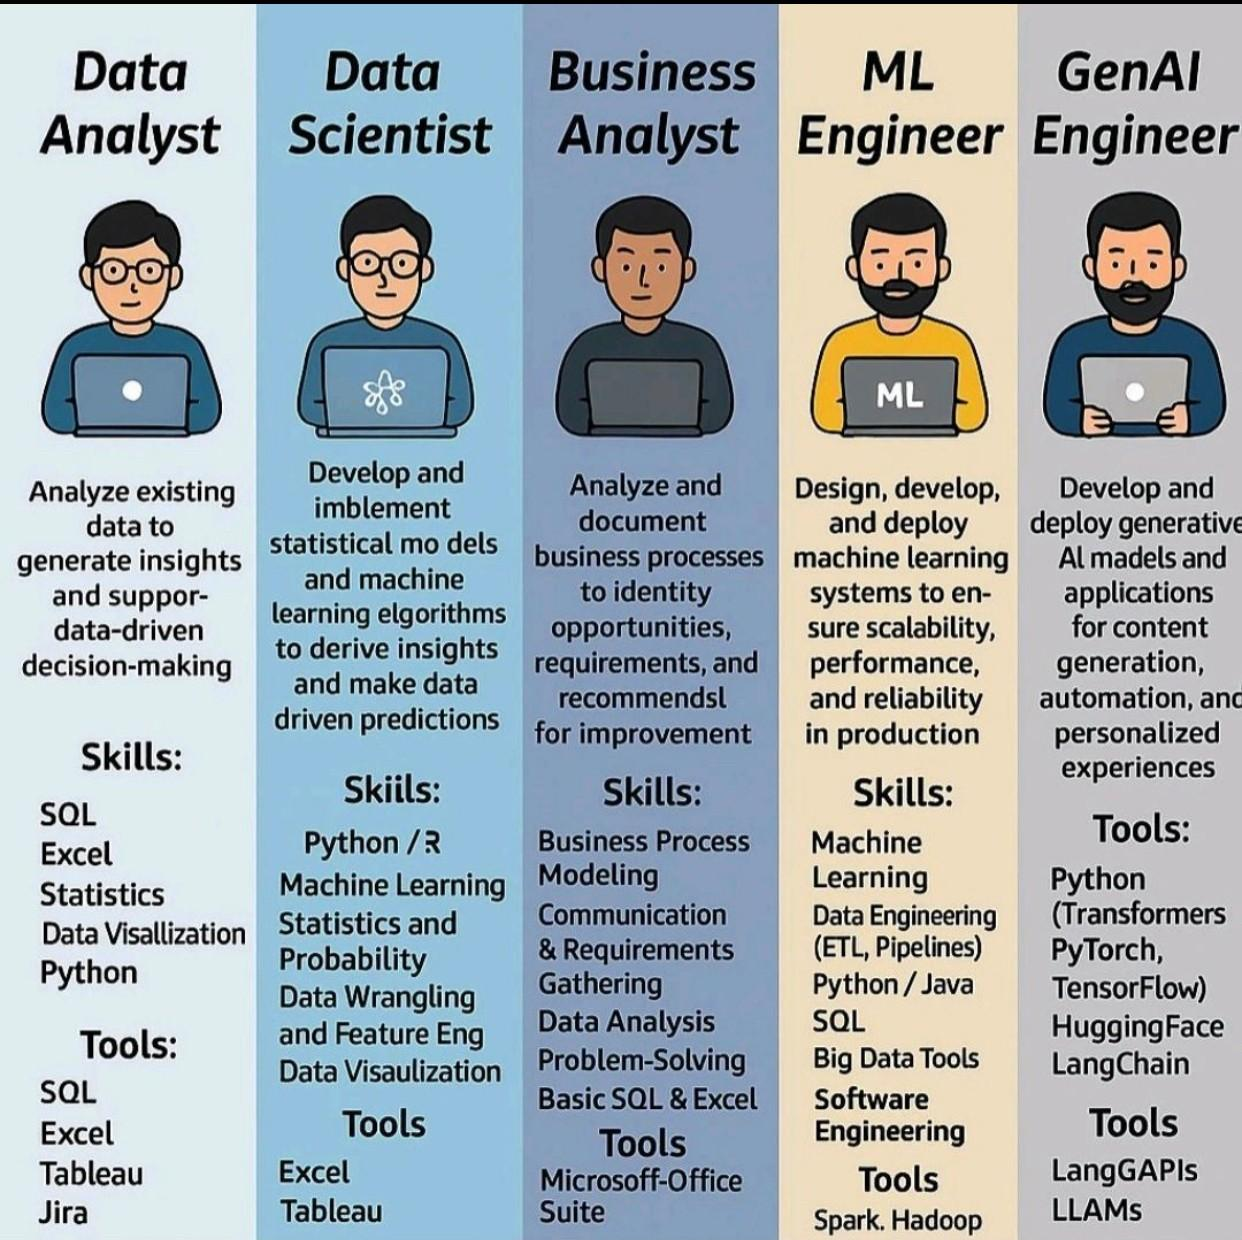
\includegraphics[width=0.6\linewidth,height=0.6\textheight]{images/role-of-datascience-ai.jpg}

}

\caption{\label{fig-roledatascience}Roles in Data Science and AI}

\end{figure}%

~~~~~A \textbf{data analyst} is a professional who collects, cleans, and
organizes data to produce insights that support business decisions. This
role typically involves working with data from multiple sources,
applying statistical and analytical techniques to identify trends and
patterns, and translating those findings into clear reports, dashboards,
and visualizations for nontechnical stakeholders. Data analysts often
collaborate closely with business teams to clarify questions, define key
performance indicators, and recommend data‑driven improvements to
processes, products, or strategies, making them a central link between
raw data and actionable decision‑making.

~~~~~A \textbf{data scientist} is a specialist who uses advanced
statistical modeling, machine learning, and programming to extract
deeper patterns and predictive insights from large, complex datasets.
Data scientists design experiments and build models, validate them using
rigorous evaluation techniques, and then deploy or operationalize these
models to support strategic decisions and automated systems. They
typically work end‑to‑end across the data lifecycle---exploring data,
engineering features, selecting algorithms, and interpreting
results---while collaborating with business stakeholders and engineering
teams to ensure that their solutions are both technically sound and
aligned with organizational goals.

\chapter{Foundations of Accounting
Data}\label{foundations-of-accounting-data}

\subsection*{Learning Objectives of the
Chapter}\label{learning-objectives-of-the-chapter-1}
\addcontentsline{toc}{subsection}{Learning Objectives of the Chapter}

\begin{tcolorbox}[enhanced jigsaw, arc=.35mm, bottomrule=.15mm, bottomtitle=1mm, breakable, colback=white, colbacktitle=quarto-callout-note-color!10!white, colframe=quarto-callout-note-color-frame, coltitle=black, left=2mm, leftrule=.75mm, opacityback=0, opacitybacktitle=0.6, rightrule=.15mm, title=\textcolor{quarto-callout-note-color}{\faInfo}\hspace{0.5em}{Learning Objectives}, titlerule=0mm, toprule=.15mm, toptitle=1mm]

At the End of the Chapter, Students should be Able to -

\begin{itemize}
\item
  Gain an understanding about the types of accounting data
\item
  Gain an understanding about the sources of accounting data
\item
  Gain an understanding how accounting data can be collected
\item
  Gain an understanding how accounting data are evolving
\item
  Collect some accounting data
\end{itemize}

\end{tcolorbox}

\section{Types of Accounting Data}\label{types-of-accounting-data}

\section{Data Sources and Collection
Methods}\label{data-sources-and-collection-methods}

\section{Data Quality \& Integrity}\label{data-quality-integrity}

summary, this book has no content whatsoever.

\begin{Shaded}
\begin{Highlighting}[]
\DecValTok{1} \SpecialCharTok{+} \DecValTok{1}
\end{Highlighting}
\end{Shaded}

\begin{verbatim}
[1] 2
\end{verbatim}

\begin{Shaded}
\begin{Highlighting}[]
\FunctionTok{plot}\NormalTok{(mtcars[}\DecValTok{1}\SpecialCharTok{:}\DecValTok{3}\NormalTok{])}
\end{Highlighting}
\end{Shaded}

\pandocbounded{
\includegraphics[keepaspectratio]{foundations_files/figure-pdf/unnamed-chunk-2-1.pdf}}

See Figure~\ref{fig-firstplot} for first ggplot graph

\begin{Shaded}
\begin{Highlighting}[]
\FunctionTok{library}\NormalTok{(tidyverse)}
\NormalTok{mtcars }\SpecialCharTok{\%\textgreater{}\%} 
  \FunctionTok{as\_tibble}\NormalTok{() }\SpecialCharTok{\%\textgreater{}\%} 
  \FunctionTok{ggplot}\NormalTok{(}\AttributeTok{mapping =} \FunctionTok{aes}\NormalTok{(}\AttributeTok{x =}\NormalTok{ mpg, }\AttributeTok{y =}\NormalTok{ disp))}\SpecialCharTok{+}
  \FunctionTok{geom\_point}\NormalTok{()}\SpecialCharTok{+}
  \FunctionTok{geom\_smooth}\NormalTok{()}\SpecialCharTok{+}
  \FunctionTok{labs}\NormalTok{(}\AttributeTok{x =} \StringTok{\textquotesingle{}Miles Per Gallon (mpg)\textquotesingle{}}\NormalTok{,}
       \AttributeTok{y =} \StringTok{\textquotesingle{}Displacement in Cubic Inches (disp)\textquotesingle{}}\NormalTok{)}
\end{Highlighting}
\end{Shaded}

\begin{figure}[H]

\centering{

\pandocbounded{
\includegraphics[keepaspectratio]{foundations_files/figure-pdf/fig-firstplot-1.pdf}}

}

\caption{\label{fig-firstplot}Scatter plot and line plot of the relation
between \texttt{mpg} and \texttt{disp}}

\end{figure}%

\begin{Shaded}
\begin{Highlighting}[]
\FunctionTok{library}\NormalTok{(lubridate)}
\end{Highlighting}
\end{Shaded}

\begin{Shaded}
\begin{Highlighting}[]
\ImportTok{import}\NormalTok{ os}
\ImportTok{import}\NormalTok{ sys}
\NormalTok{sys.version}
\end{Highlighting}
\end{Shaded}

\begin{verbatim}
'3.11.0 (main, Oct 24 2022, 18:26:48) [MSC v.1933 64 bit (AMD64)]'
\end{verbatim}

\begin{Shaded}
\begin{Highlighting}[]
\ControlFlowTok{for}\NormalTok{ x }\KeywordTok{in}\NormalTok{ os.listdir():}
  \BuiltInTok{print}\NormalTok{ (x)}
\end{Highlighting}
\end{Shaded}

\begin{verbatim}
.env
.git
.gitattributes
.gitignore
.quarto
.README.md.swp
.README_BASE_1260.md.swp
.README_LOCAL_1260.md.swp
.README_REMOTE_1260.md.swp
.Rhistory
.vdoc.b7f6298e-a6af-42d8-806b-03c5619ab147.py
accounting_analytics_book
advanced_analytics.html
advanced_analytics.qmd
advanced_analytics.quarto_ipynb
advanced_analytics.quarto_ipynb_1
advanced_analytics.quarto_ipynb_2
advanced_analytics.quarto_ipynb_3
advanced_analytics.quarto_ipynb_4
advanced_analytics.quarto_ipynb_5
advanced_analytics.quarto_ipynb_6
advanced_analytics.quarto_ipynb_7
advanced_analytics.quarto_ipynb_8
chapter1_solution.html
chapter1_solution.qmd
chapter2_solution.html
chapter2_solution.qmd
cover.png
dashboard.html
dashboard.qmd
dashboard.quarto_ipynb
dashboard.quarto_ipynb_1
dashboard.quarto_ipynb_2
dashboard.quarto_ipynb_3
dashboard.quarto_ipynb_4
dashboard.quarto_ipynb_5
dashboard.quarto_ipynb_6
dashboard.quarto_ipynb_7
dashboard.quarto_ipynb_8
DATA
data_management.html
data_management.qmd
eda.html
eda.qmd
ethics.html
ethics.qmd
file3e9c78b886c
file6ed81b1d1d61
file729017a834a5
foundations.html
foundations.qmd
foundations.rmarkdown
foundations_files
fraud.html
fraud.qmd
future.html
future.qmd
images
index.aux
index.html
index.log
index.pdf
index.qmd
index.tex
index.toc
intro.qmd
machine_learning.html
machine_learning.qmd
machine_learning.quarto_ipynb
machine_learning.quarto_ipynb_1
machine_learning.quarto_ipynb_2
machine_learning.quarto_ipynb_3
machine_learning.quarto_ipynb_4
machine_learning.quarto_ipynb_5
machine_learning.quarto_ipynb_6
machine_learning.quarto_ipynb_7
machine_learning.quarto_ipynb_8
machine_learning_files
nlp.html
nlp.qmd
nlp.quarto_ipynb
nlp.quarto_ipynb_1
nlp.quarto_ipynb_2
nlp.quarto_ipynb_3
nlp.quarto_ipynb_4
nlp.quarto_ipynb_5
nlp.quarto_ipynb_6
nlp.quarto_ipynb_7
nlp.quarto_ipynb_8
nlp_files
overview.html
overview.qmd
performance_measurement.html
performance_measurement.qmd
predictive.html
predictive.ipynb
predictive.qmd
predictive_files
prescriptive.html
prescriptive.qmd
python_basics.html
python_basics.qmd
python_basics.quarto_ipynb
python_basics.quarto_ipynb_1
python_basics.quarto_ipynb_2
python_basics.quarto_ipynb_3
python_basics.quarto_ipynb_4
python_basics.quarto_ipynb_5
python_basics.quarto_ipynb_6
python_basics.quarto_ipynb_7
python_basics.quarto_ipynb_8
python_version_used.txt
README.html
README.md
README_files
references.bib
references.html
references.qmd
requirements.txt
r_basics.html
r_basics.qmd
r_basics_files
site_libs
visualization.html
visualization.qmd
visualization_files
_book
_quarto.yml
\end{verbatim}

\part{Data Exploration and Management}

\chapter{Exploratory Data Analysis
(EDA)}\label{exploratory-data-analysis-eda}

\subsection*{Learning Objectives of the
Chapter}\label{learning-objectives-of-the-chapter-2}
\addcontentsline{toc}{subsection}{Learning Objectives of the Chapter}

\begin{tcolorbox}[enhanced jigsaw, arc=.35mm, bottomrule=.15mm, bottomtitle=1mm, breakable, colback=white, colbacktitle=quarto-callout-note-color!10!white, colframe=quarto-callout-note-color-frame, coltitle=black, left=2mm, leftrule=.75mm, opacityback=0, opacitybacktitle=0.6, rightrule=.15mm, title=\textcolor{quarto-callout-note-color}{\faInfo}\hspace{0.5em}{Learning Objectives}, titlerule=0mm, toprule=.15mm, toptitle=1mm]

At the End of the Chapter, Students should be Able to -

\begin{itemize}
\item
  Learn about the purpose of Exploratory Data Analysis (EDA)
\item
  Understand different techniques of transforming and cleaning data
\item
  Learn about Different R and Python Packages for EDA
\item
  Understand how to use six verbs for EDA
\item
  Perform EDA on some real world data sets
\item
  Learn about how to interpret results from EDA
\end{itemize}

\end{tcolorbox}

\section{Introduction}\label{introduction}

~~~~~Exploratory Data Analysis (EDA) is the initial process of examining
a dataset to understand its main characteristics before applying formal
statistical models or machine learning algorithms. It typically combines
summary statistics with visual tools such as histograms, boxplots, and
scatterplots to uncover patterns, spot anomalies, test assumptions, and
check data quality.

~~~~~By revealing relationships among variables, distributions, and
potential outliers, EDA helps refine research questions, choose
appropriate modeling techniques, and prevent misleading conclusions. In
this way, EDA acts as a bridge between raw data and rigorous analysis,
ensuring that subsequent steps are grounded in an accurate and
transparent understanding of the underlying information.

\section{Data Collection \& Importing}\label{data-collection-importing}

\section{Data Cleaning}\label{data-cleaning}

\section{Packages for Exploratory Data Analysis
(EDA)}\label{packages-for-exploratory-data-analysis-eda}

~~~~~In order to use \texttt{pyjanitor}, the data frame must be pandas
because \texttt{pyjanitor} extends pandas data frame functionality.

\section{dplyr}

\begin{Shaded}
\begin{Highlighting}[]
\CommentTok{\# loading packages}
\FunctionTok{library}\NormalTok{(tidyverse)}
\FunctionTok{library}\NormalTok{(lubridate)}
\FunctionTok{library}\NormalTok{(janitor)}
\end{Highlighting}
\end{Shaded}

\section{pandas}

\begin{Shaded}
\begin{Highlighting}[]
\CommentTok{\# loading the package}
\ImportTok{import}\NormalTok{ numpy }\ImportTok{as}\NormalTok{ np}
\ImportTok{import}\NormalTok{ pandas }\ImportTok{as}\NormalTok{ pd}
\CommentTok{\# from pyjanitor package }
\CommentTok{\# pip install pyjanitor}
\ImportTok{import}\NormalTok{ janitor }
\ImportTok{from}\NormalTok{ janitor }\ImportTok{import}\NormalTok{ clean\_names, remove\_empty}
\end{Highlighting}
\end{Shaded}

\section{polars}

\begin{Shaded}
\begin{Highlighting}[]
\CommentTok{\# loading the package }
\ImportTok{import}\NormalTok{ polars }\ImportTok{as}\NormalTok{ pl}
\end{Highlighting}
\end{Shaded}

\section{Importing the Dataset}\label{importing-the-dataset}

\section{dplyr}

\begin{Shaded}
\begin{Highlighting}[]
\CommentTok{\# importing data frame }
\NormalTok{df }\OtherTok{=} \FunctionTok{read\_csv}\NormalTok{(}\StringTok{"https://raw.githubusercontent.com/msharifbd/DATA/main/Al{-}Bundy\_raw{-}data.csv"}\NormalTok{)}
\end{Highlighting}
\end{Shaded}

\section{pandas}

\begin{Shaded}
\begin{Highlighting}[]
\CommentTok{\# importing data frame }
\NormalTok{df\_pd }\OperatorTok{=}\NormalTok{ pd.read\_csv(}\StringTok{"https://raw.githubusercontent.com/msharifbd/DATA/main/Al{-}Bundy\_raw{-}data.csv"}\NormalTok{)}
\end{Highlighting}
\end{Shaded}

\section{polars}

\begin{Shaded}
\begin{Highlighting}[]
\CommentTok{\# importing data frame }
\NormalTok{df\_pl }\OperatorTok{=}\NormalTok{ pl.read\_csv(}\StringTok{"https://raw.githubusercontent.com/msharifbd/DATA/main/Al{-}Bundy\_raw{-}data.csv"}\NormalTok{)}
\end{Highlighting}
\end{Shaded}

\section{Meta Data}\label{meta-data}

~~~~~Meta data is data about the data. Before we put the data into
analysis, we need to learn about our dataset. This learning invovles
knowing about the number of rows, number of columns, the types of the
fields, the appropriateness of those types, the missing values in the
dataset and so on.

\section{dplyr}

\begin{Shaded}
\begin{Highlighting}[]
\FunctionTok{glimpse}\NormalTok{(df)}
\end{Highlighting}
\end{Shaded}

\begin{verbatim}
Rows: 14,967
Columns: 14
$ InvoiceNo       <dbl> 52389, 52390, 52391, 52392, 52393, 52394, 52395, 52396~
$ Date            <chr> "1/1/2014", "1/1/2014", "1/1/2014", "1/1/2014", "1/1/2~
$ Country         <chr> "United Kingdom", "United States", "Canada", "United S~
$ ProductID       <dbl> 2152, 2230, 2160, 2234, 2222, 2173, 2200, 2238, 2191, ~
$ Shop            <chr> "UK2", "US15", "CAN7", "US6", "UK4", "US15", "GER2", "~
$ Gender          <chr> "Male", "Male", "Male", "Female", "Female", "Male", "F~
$ `Size (US)`     <dbl> 11.0, 11.5, 9.5, 9.5, 9.0, 10.5, 9.0, 10.0, 10.5, 9.0,~
$ `Size (Europe)` <chr> "44", "44-45", "42-43", "40", "39-40", "43-44", "39-40~
$ `Size (UK)`     <dbl> 10.5, 11.0, 9.0, 7.5, 7.0, 10.0, 7.0, 9.5, 10.0, 7.0, ~
$ UnitPrice       <dbl> 159, 199, 149, 159, 159, 159, 179, 169, 139, 149, 129,~
$ Discount        <dbl> 0.0, 0.2, 0.2, 0.0, 0.0, 0.0, 0.0, 0.0, 0.0, 0.0, 0.0,~
$ Year            <dbl> 2014, 2014, 2014, 2014, 2014, 2014, 2014, 2014, 2014, ~
$ Month           <dbl> 1, 1, 1, 1, 1, 1, 1, 1, 1, 1, 1, 1, 1, 1, 1, 1, 1, 1, ~
$ SalePrice       <dbl> 159.0, 159.2, 119.2, 159.0, 159.0, 159.0, 179.0, 169.0~
\end{verbatim}

\begin{Shaded}
\begin{Highlighting}[]
\FunctionTok{map\_df}\NormalTok{(df, }\SpecialCharTok{\textasciitilde{}}\FunctionTok{sum}\NormalTok{(}\FunctionTok{is.na}\NormalTok{(.))) }\SpecialCharTok{|\textgreater{}}
     \FunctionTok{glimpse}\NormalTok{()}
\end{Highlighting}
\end{Shaded}

\begin{verbatim}
Rows: 1
Columns: 14
$ InvoiceNo       <int> 0
$ Date            <int> 0
$ Country         <int> 0
$ ProductID       <int> 0
$ Shop            <int> 0
$ Gender          <int> 0
$ `Size (US)`     <int> 0
$ `Size (Europe)` <int> 0
$ `Size (UK)`     <int> 0
$ UnitPrice       <int> 0
$ Discount        <int> 0
$ Year            <int> 0
$ Month           <int> 0
$ SalePrice       <int> 0
\end{verbatim}

\begin{Shaded}
\begin{Highlighting}[]
\FunctionTok{ncol}\NormalTok{(df)}
\end{Highlighting}
\end{Shaded}

\begin{verbatim}
[1] 14
\end{verbatim}

\begin{Shaded}
\begin{Highlighting}[]
\FunctionTok{nrow}\NormalTok{(df)}
\end{Highlighting}
\end{Shaded}

\begin{verbatim}
[1] 14967
\end{verbatim}

\begin{Shaded}
\begin{Highlighting}[]
\FunctionTok{head}\NormalTok{(df)}
\end{Highlighting}
\end{Shaded}

\begin{verbatim}
# A tibble: 6 x 14
  InvoiceNo Date     Country  ProductID Shop  Gender `Size (US)` `Size (Europe)`
      <dbl> <chr>    <chr>        <dbl> <chr> <chr>        <dbl> <chr>          
1     52389 1/1/2014 United ~      2152 UK2   Male          11   44             
2     52390 1/1/2014 United ~      2230 US15  Male          11.5 44-45          
3     52391 1/1/2014 Canada        2160 CAN7  Male           9.5 42-43          
4     52392 1/1/2014 United ~      2234 US6   Female         9.5 40             
5     52393 1/1/2014 United ~      2222 UK4   Female         9   39-40          
6     52394 1/1/2014 United ~      2173 US15  Male          10.5 43-44          
# i 6 more variables: `Size (UK)` <dbl>, UnitPrice <dbl>, Discount <dbl>,
#   Year <dbl>, Month <dbl>, SalePrice <dbl>
\end{verbatim}

\begin{Shaded}
\begin{Highlighting}[]
\FunctionTok{tail}\NormalTok{(df)}
\end{Highlighting}
\end{Shaded}

\begin{verbatim}
# A tibble: 6 x 14
  InvoiceNo Date      Country ProductID Shop  Gender `Size (US)` `Size (Europe)`
      <dbl> <chr>     <chr>       <dbl> <chr> <chr>        <dbl> <chr>          
1     65772 12/31/20~ United~      2168 US13  Male           8   41             
2     65773 12/31/20~ United~      2154 UK2   Male           9.5 42-43          
3     65774 12/31/20~ United~      2181 US12  Female        12   42-43          
4     65775 12/31/20~ Canada       2203 CAN6  Male          10.5 43-44          
5     65776 12/31/20~ Germany      2231 GER1  Female         9.5 40             
6     65777 12/31/20~ Germany      2156 GER1  Female         6.5 37             
# i 6 more variables: `Size (UK)` <dbl>, UnitPrice <dbl>, Discount <dbl>,
#   Year <dbl>, Month <dbl>, SalePrice <dbl>
\end{verbatim}

\begin{Shaded}
\begin{Highlighting}[]
\NormalTok{dplyr}\SpecialCharTok{::}\FunctionTok{sample\_n}\NormalTok{(df, }\DecValTok{10}\NormalTok{)}
\end{Highlighting}
\end{Shaded}

\begin{verbatim}
# A tibble: 10 x 14
   InvoiceNo Date     Country ProductID Shop  Gender `Size (US)` `Size (Europe)`
       <dbl> <chr>    <chr>       <dbl> <chr> <chr>        <dbl> <chr>          
 1     63768 9/7/2016 Germany      2242 GER1  Female         7.5 38             
 2     58683 11/24/2~ Canada       2149 CAN5  Female         7   37-38          
 3     63977 9/17/20~ Germany      2163 GER1  Male          10.5 43-44          
 4     60327 3/11/20~ United~      2234 US14  Female        11.5 42             
 5     63743 9/6/2016 Canada       2182 CAN1  Female        10   40-41          
 6     59805 2/8/2016 United~      2166 US13  Female         7.5 38             
 7     61504 5/18/20~ Germany      2164 GER1  Female         9.5 40             
 8     55037 2/2/2015 United~      2171 US9   Male          10.5 43-44          
 9     59913 2/15/20~ Germany      2241 GER1  Male          11   44             
10     61861 6/7/2016 United~      2177 US13  Male           9.5 42-43          
# i 6 more variables: `Size (UK)` <dbl>, UnitPrice <dbl>, Discount <dbl>,
#   Year <dbl>, Month <dbl>, SalePrice <dbl>
\end{verbatim}

\section{Pandas}

\begin{Shaded}
\begin{Highlighting}[]
\NormalTok{df\_pd.info()}
\end{Highlighting}
\end{Shaded}

\begin{verbatim}
<class 'pandas.core.frame.DataFrame'>
RangeIndex: 14967 entries, 0 to 14966
Data columns (total 14 columns):
 #   Column         Non-Null Count  Dtype  
---  ------         --------------  -----  
 0   InvoiceNo      14967 non-null  int64  
 1   Date           14967 non-null  object 
 2   Country        14967 non-null  object 
 3   ProductID      14967 non-null  int64  
 4   Shop           14967 non-null  object 
 5   Gender         14967 non-null  object 
 6   Size (US)      14967 non-null  float64
 7   Size (Europe)  14967 non-null  object 
 8   Size (UK)      14967 non-null  float64
 9   UnitPrice      14967 non-null  int64  
 10  Discount       14967 non-null  float64
 11  Year           14967 non-null  int64  
 12  Month          14967 non-null  int64  
 13  SalePrice      14967 non-null  float64
dtypes: float64(4), int64(5), object(5)
memory usage: 1.6+ MB
\end{verbatim}

\begin{Shaded}
\begin{Highlighting}[]
\NormalTok{df\_pd.shape}
\end{Highlighting}
\end{Shaded}

\begin{verbatim}
(14967, 14)
\end{verbatim}

\begin{Shaded}
\begin{Highlighting}[]
\BuiltInTok{print}\NormalTok{(}\StringTok{\textquotesingle{}The total number of rows and columns of the product data is }\OperatorTok{\textbackslash{}}
\StringTok{ }\SpecialCharTok{\{\}}\StringTok{ and }\SpecialCharTok{\{\}}\StringTok{ respectively.\textquotesingle{}}\NormalTok{.}\BuiltInTok{format}\NormalTok{(df\_pd.shape[}\DecValTok{0}\NormalTok{], df\_pd.shape[}\DecValTok{1}\NormalTok{]))}
\end{Highlighting}
\end{Shaded}

\begin{verbatim}
The total number of rows and columns of the product data is  14967 and 14 respectively.
\end{verbatim}

\begin{Shaded}
\begin{Highlighting}[]
\BuiltInTok{print}\NormalTok{(}\SpecialStringTok{f\textquotesingle{}The total number of rows and columns of the product data is }\OperatorTok{\textbackslash{}}
\SpecialStringTok{ }\SpecialCharTok{\{}\NormalTok{df\_pd}\SpecialCharTok{.}\NormalTok{shape[}\DecValTok{0}\NormalTok{]}\SpecialCharTok{\}}\SpecialStringTok{ and }\SpecialCharTok{\{}\NormalTok{df\_pd}\SpecialCharTok{.}\NormalTok{shape[}\DecValTok{1}\NormalTok{]}\SpecialCharTok{\}}\SpecialStringTok{ respectively.\textquotesingle{}}\NormalTok{)}
\end{Highlighting}
\end{Shaded}

\begin{verbatim}
The total number of rows and columns of the product data is  14967 and 14 respectively.
\end{verbatim}

\begin{Shaded}
\begin{Highlighting}[]
\NormalTok{df\_pd.columns}
\end{Highlighting}
\end{Shaded}

\begin{verbatim}
Index(['InvoiceNo', 'Date', 'Country', 'ProductID', 'Shop', 'Gender',
       'Size (US)', 'Size (Europe)', 'Size (UK)', 'UnitPrice', 'Discount',
       'Year', 'Month', 'SalePrice'],
      dtype='object')
\end{verbatim}

\begin{Shaded}
\begin{Highlighting}[]
\NormalTok{df\_pd.head()}
\end{Highlighting}
\end{Shaded}

\begin{verbatim}
   InvoiceNo      Date         Country  ...  Year Month SalePrice
0      52389  1/1/2014  United Kingdom  ...  2014     1     159.0
1      52390  1/1/2014   United States  ...  2014     1     159.2
2      52391  1/1/2014          Canada  ...  2014     1     119.2
3      52392  1/1/2014   United States  ...  2014     1     159.0
4      52393  1/1/2014  United Kingdom  ...  2014     1     159.0

[5 rows x 14 columns]
\end{verbatim}

\begin{Shaded}
\begin{Highlighting}[]
\NormalTok{df\_pd.tail()}
\end{Highlighting}
\end{Shaded}

\begin{verbatim}
       InvoiceNo        Date         Country  ...  Year Month SalePrice
14962      65773  12/31/2016  United Kingdom  ...  2016    12     139.0
14963      65774  12/31/2016   United States  ...  2016    12     149.0
14964      65775  12/31/2016          Canada  ...  2016    12     125.3
14965      65776  12/31/2016         Germany  ...  2016    12     199.0
14966      65777  12/31/2016         Germany  ...  2016    12     125.1

[5 rows x 14 columns]
\end{verbatim}

\begin{Shaded}
\begin{Highlighting}[]
\NormalTok{df\_pd.isna().}\BuiltInTok{sum}\NormalTok{()}
\end{Highlighting}
\end{Shaded}

\begin{verbatim}
InvoiceNo        0
Date             0
Country          0
ProductID        0
Shop             0
Gender           0
Size (US)        0
Size (Europe)    0
Size (UK)        0
UnitPrice        0
Discount         0
Year             0
Month            0
SalePrice        0
dtype: int64
\end{verbatim}

\begin{Shaded}
\begin{Highlighting}[]
\NormalTok{df\_pd.dtypes}
\end{Highlighting}
\end{Shaded}

\begin{verbatim}
InvoiceNo          int64
Date              object
Country           object
ProductID          int64
Shop              object
Gender            object
Size (US)        float64
Size (Europe)     object
Size (UK)        float64
UnitPrice          int64
Discount         float64
Year               int64
Month              int64
SalePrice        float64
dtype: object
\end{verbatim}

\begin{Shaded}
\begin{Highlighting}[]
\NormalTok{df\_pd.sample(n}\OperatorTok{=}\DecValTok{10}\NormalTok{)}
\end{Highlighting}
\end{Shaded}

\begin{verbatim}
       InvoiceNo        Date         Country  ...  Year Month SalePrice
10887      62123   6/20/2016   United States  ...  2016     6     139.0
10805      62052   6/17/2016   United States  ...  2016     6     179.0
12822      63838   9/11/2016         Germany  ...  2016     9     135.2
4018       55904   4/30/2015   United States  ...  2015     4     152.1
3733       55640    4/4/2015          Canada  ...  2015     4     135.2
7458       59070  12/21/2015         Germany  ...  2015    12     189.0
10884      62120   6/20/2016  United Kingdom  ...  2016     6     159.0
5307       57082   7/30/2015   United States  ...  2015     7     139.3
14662      65492  12/11/2016         Germany  ...  2016    12     111.2
10348      61646   5/26/2016   United States  ...  2016     5     199.0

[10 rows x 14 columns]
\end{verbatim}

\section{polars}

\begin{Shaded}
\begin{Highlighting}[]
\CommentTok{\# metadata}
\NormalTok{df\_pl.shape }\CommentTok{\# rows and columns}
\end{Highlighting}
\end{Shaded}

\begin{verbatim}
(14967, 14)
\end{verbatim}

\begin{Shaded}
\begin{Highlighting}[]
\NormalTok{df\_pl.height }\CommentTok{\# rows}
\end{Highlighting}
\end{Shaded}

\begin{verbatim}
14967
\end{verbatim}

\begin{Shaded}
\begin{Highlighting}[]
\NormalTok{df\_pl.width }\CommentTok{\# columns }
\end{Highlighting}
\end{Shaded}

\begin{verbatim}
14
\end{verbatim}

\begin{Shaded}
\begin{Highlighting}[]
\NormalTok{df\_pl.columns}
\end{Highlighting}
\end{Shaded}

\begin{verbatim}
['InvoiceNo', 'Date', 'Country', 'ProductID', 'Shop', 'Gender', 'Size (US)', 'Size (Europe)', 'Size (UK)', 'UnitPrice', 'Discount', 'Year', 'Month', 'SalePrice']
\end{verbatim}

\begin{Shaded}
\begin{Highlighting}[]
\BuiltInTok{len}\NormalTok{(df\_pl.columns)}
\end{Highlighting}
\end{Shaded}

\begin{verbatim}
14
\end{verbatim}

\begin{Shaded}
\begin{Highlighting}[]
\NormalTok{df\_pl.schema }\CommentTok{\# column names and their types }
\end{Highlighting}
\end{Shaded}

\begin{verbatim}
Schema([('InvoiceNo', Int64), ('Date', String), ('Country', String), ('ProductID', Int64), ('Shop', String), ('Gender', String), ('Size (US)', Float64), ('Size (Europe)', String), ('Size (UK)', Float64), ('UnitPrice', Int64), ('Discount', Float64), ('Year', Int64), ('Month', Int64), ('SalePrice', Float64)])
\end{verbatim}

\begin{Shaded}
\begin{Highlighting}[]
\NormalTok{df\_pl.dtypes}
\end{Highlighting}
\end{Shaded}

\begin{verbatim}
[Int64, String, String, Int64, String, String, Float64, String, Float64, Int64, Float64, Int64, Int64, Float64]
\end{verbatim}

\begin{Shaded}
\begin{Highlighting}[]
\NormalTok{df\_pl.head()}
\end{Highlighting}
\end{Shaded}

\begin{verbatim}
shape: (5, 14)
┌───────────┬──────────┬────────────────┬───────────┬───┬──────────┬──────┬───────┬───────────┐
│ InvoiceNo ┆ Date     ┆ Country        ┆ ProductID ┆ … ┆ Discount ┆ Year ┆ Month ┆ SalePrice │
│ ---       ┆ ---      ┆ ---            ┆ ---       ┆   ┆ ---      ┆ ---  ┆ ---   ┆ ---       │
│ i64       ┆ str      ┆ str            ┆ i64       ┆   ┆ f64      ┆ i64  ┆ i64   ┆ f64       │
╞═══════════╪══════════╪════════════════╪═══════════╪═══╪══════════╪══════╪═══════╪═══════════╡
│ 52389     ┆ 1/1/2014 ┆ United Kingdom ┆ 2152      ┆ … ┆ 0.0      ┆ 2014 ┆ 1     ┆ 159.0     │
│ 52390     ┆ 1/1/2014 ┆ United States  ┆ 2230      ┆ … ┆ 0.2      ┆ 2014 ┆ 1     ┆ 159.2     │
│ 52391     ┆ 1/1/2014 ┆ Canada         ┆ 2160      ┆ … ┆ 0.2      ┆ 2014 ┆ 1     ┆ 119.2     │
│ 52392     ┆ 1/1/2014 ┆ United States  ┆ 2234      ┆ … ┆ 0.0      ┆ 2014 ┆ 1     ┆ 159.0     │
│ 52393     ┆ 1/1/2014 ┆ United Kingdom ┆ 2222      ┆ … ┆ 0.0      ┆ 2014 ┆ 1     ┆ 159.0     │
└───────────┴──────────┴────────────────┴───────────┴───┴──────────┴──────┴───────┴───────────┘
\end{verbatim}

\begin{Shaded}
\begin{Highlighting}[]
\NormalTok{df\_pl.tail()}
\end{Highlighting}
\end{Shaded}

\begin{verbatim}
shape: (5, 14)
┌───────────┬────────────┬────────────────┬───────────┬───┬──────────┬──────┬───────┬───────────┐
│ InvoiceNo ┆ Date       ┆ Country        ┆ ProductID ┆ … ┆ Discount ┆ Year ┆ Month ┆ SalePrice │
│ ---       ┆ ---        ┆ ---            ┆ ---       ┆   ┆ ---      ┆ ---  ┆ ---   ┆ ---       │
│ i64       ┆ str        ┆ str            ┆ i64       ┆   ┆ f64      ┆ i64  ┆ i64   ┆ f64       │
╞═══════════╪════════════╪════════════════╪═══════════╪═══╪══════════╪══════╪═══════╪═══════════╡
│ 65773     ┆ 12/31/2016 ┆ United Kingdom ┆ 2154      ┆ … ┆ 0.0      ┆ 2016 ┆ 12    ┆ 139.0     │
│ 65774     ┆ 12/31/2016 ┆ United States  ┆ 2181      ┆ … ┆ 0.0      ┆ 2016 ┆ 12    ┆ 149.0     │
│ 65775     ┆ 12/31/2016 ┆ Canada         ┆ 2203      ┆ … ┆ 0.3      ┆ 2016 ┆ 12    ┆ 125.3     │
│ 65776     ┆ 12/31/2016 ┆ Germany        ┆ 2231      ┆ … ┆ 0.0      ┆ 2016 ┆ 12    ┆ 199.0     │
│ 65777     ┆ 12/31/2016 ┆ Germany        ┆ 2156      ┆ … ┆ 0.1      ┆ 2016 ┆ 12    ┆ 125.1     │
└───────────┴────────────┴────────────────┴───────────┴───┴──────────┴──────┴───────┴───────────┘
\end{verbatim}

\begin{Shaded}
\begin{Highlighting}[]
\NormalTok{df\_pl.sample(n}\OperatorTok{=}\DecValTok{10}\NormalTok{)}
\end{Highlighting}
\end{Shaded}

\begin{verbatim}
shape: (10, 14)
┌───────────┬────────────┬───────────────┬───────────┬───┬──────────┬──────┬───────┬───────────┐
│ InvoiceNo ┆ Date       ┆ Country       ┆ ProductID ┆ … ┆ Discount ┆ Year ┆ Month ┆ SalePrice │
│ ---       ┆ ---        ┆ ---           ┆ ---       ┆   ┆ ---      ┆ ---  ┆ ---   ┆ ---       │
│ i64       ┆ str        ┆ str           ┆ i64       ┆   ┆ f64      ┆ i64  ┆ i64   ┆ f64       │
╞═══════════╪════════════╪═══════════════╪═══════════╪═══╪══════════╪══════╪═══════╪═══════════╡
│ 60373     ┆ 3/13/2016  ┆ United States ┆ 2177      ┆ … ┆ 0.0      ┆ 2016 ┆ 3     ┆ 169.0     │
│ 52719     ┆ 2/25/2014  ┆ Canada        ┆ 2212      ┆ … ┆ 0.0      ┆ 2014 ┆ 2     ┆ 149.0     │
│ 62775     ┆ 7/21/2016  ┆ Germany       ┆ 2164      ┆ … ┆ 0.3      ┆ 2016 ┆ 7     ┆ 104.3     │
│ 52437     ┆ 1/8/2014   ┆ United States ┆ 2207      ┆ … ┆ 0.0      ┆ 2014 ┆ 1     ┆ 169.0     │
│ 52815     ┆ 3/12/2014  ┆ United States ┆ 2159      ┆ … ┆ 0.0      ┆ 2014 ┆ 3     ┆ 179.0     │
│ 59612     ┆ 1/27/2016  ┆ Canada        ┆ 2229      ┆ … ┆ 0.0      ┆ 2016 ┆ 1     ┆ 159.0     │
│ 55536     ┆ 3/24/2015  ┆ United States ┆ 2207      ┆ … ┆ 0.1      ┆ 2015 ┆ 3     ┆ 179.1     │
│ 56012     ┆ 5/11/2015  ┆ United States ┆ 2200      ┆ … ┆ 0.0      ┆ 2015 ┆ 5     ┆ 199.0     │
│ 65640     ┆ 12/21/2016 ┆ Canada        ┆ 2235      ┆ … ┆ 0.0      ┆ 2016 ┆ 12    ┆ 199.0     │
│ 60332     ┆ 3/11/2016  ┆ Germany       ┆ 2230      ┆ … ┆ 0.5      ┆ 2016 ┆ 3     ┆ 94.5      │
└───────────┴────────────┴───────────────┴───────────┴───┴──────────┴──────┴───────┴───────────┘
\end{verbatim}

\begin{Shaded}
\begin{Highlighting}[]
\NormalTok{df\_pl.describe()}
\end{Highlighting}
\end{Shaded}

\begin{verbatim}
shape: (9, 15)
┌────────────┬────────────┬──────────┬───────────┬───┬──────────┬───────────┬──────────┬───────────┐
│ statistic  ┆ InvoiceNo  ┆ Date     ┆ Country   ┆ … ┆ Discount ┆ Year      ┆ Month    ┆ SalePrice │
│ ---        ┆ ---        ┆ ---      ┆ ---       ┆   ┆ ---      ┆ ---       ┆ ---      ┆ ---       │
│ str        ┆ f64        ┆ str      ┆ str       ┆   ┆ f64      ┆ f64       ┆ f64      ┆ f64       │
╞════════════╪════════════╪══════════╪═══════════╪═══╪══════════╪═══════════╪══════════╪═══════════╡
│ count      ┆ 14967.0    ┆ 14967    ┆ 14967     ┆ … ┆ 14967.0  ┆ 14967.0   ┆ 14967.0  ┆ 14967.0   │
│ null_count ┆ 0.0        ┆ 0        ┆ 0         ┆ … ┆ 0.0      ┆ 0.0       ┆ 0.0      ┆ 0.0       │
│ mean       ┆ 59050.2615 ┆ null     ┆ null      ┆ … ┆ 0.124013 ┆ 2015.3082 ┆ 6.689517 ┆ 143.98791 │
│            ┆ 09         ┆          ┆           ┆   ┆          ┆ 11        ┆          ┆ 3         │
│ std        ┆ 3889.59871 ┆ null     ┆ null      ┆ … ┆ 0.170112 ┆ 0.76232   ┆ 3.319909 ┆ 35.180799 │
│            ┆ 4          ┆          ┆           ┆   ┆          ┆           ┆          ┆           │
│ min        ┆ 52389.0    ┆ 1/1/2014 ┆ Canada    ┆ … ┆ 0.0      ┆ 2014.0    ┆ 1.0      ┆ 64.5      │
│ 25%        ┆ 55649.0    ┆ null     ┆ null      ┆ … ┆ 0.0      ┆ 2015.0    ┆ 4.0      ┆ 125.1     │
│ 50%        ┆ 59092.0    ┆ null     ┆ null      ┆ … ┆ 0.0      ┆ 2015.0    ┆ 7.0      ┆ 149.0     │
│ 75%        ┆ 62433.0    ┆ null     ┆ null      ┆ … ┆ 0.2      ┆ 2016.0    ┆ 10.0     ┆ 169.0     │
│ max        ┆ 65777.0    ┆ 9/9/2016 ┆ United    ┆ … ┆ 0.5      ┆ 2016.0    ┆ 12.0     ┆ 199.0     │
│            ┆            ┆          ┆ States    ┆   ┆          ┆           ┆          ┆           │
└────────────┴────────────┴──────────┴───────────┴───┴──────────┴───────────┴──────────┴───────────┘
\end{verbatim}

\section{Cleaning the Dataset}\label{cleaning-the-dataset}

\section{dplyr}

\begin{Shaded}
\begin{Highlighting}[]
\NormalTok{ df }\SpecialCharTok{|\textgreater{}}
     \FunctionTok{rename\_all}\NormalTok{(toupper) }\SpecialCharTok{|\textgreater{}}
\NormalTok{     janitor}\SpecialCharTok{::}\FunctionTok{clean\_names}\NormalTok{() }\SpecialCharTok{|\textgreater{}}
     \FunctionTok{rename\_all}\NormalTok{(toupper) }\SpecialCharTok{|\textgreater{}}
     \FunctionTok{glimpse}\NormalTok{()}
\end{Highlighting}
\end{Shaded}

\begin{verbatim}
Rows: 14,967
Columns: 14
$ INVOICENO   <dbl> 52389, 52390, 52391, 52392, 52393, 52394, 52395, 52396, 52~
$ DATE        <chr> "1/1/2014", "1/1/2014", "1/1/2014", "1/1/2014", "1/1/2014"~
$ COUNTRY     <chr> "United Kingdom", "United States", "Canada", "United State~
$ PRODUCTID   <dbl> 2152, 2230, 2160, 2234, 2222, 2173, 2200, 2238, 2191, 2237~
$ SHOP        <chr> "UK2", "US15", "CAN7", "US6", "UK4", "US15", "GER2", "CAN5~
$ GENDER      <chr> "Male", "Male", "Male", "Female", "Female", "Male", "Femal~
$ SIZE_US     <dbl> 11.0, 11.5, 9.5, 9.5, 9.0, 10.5, 9.0, 10.0, 10.5, 9.0, 10.~
$ SIZE_EUROPE <chr> "44", "44-45", "42-43", "40", "39-40", "43-44", "39-40", "~
$ SIZE_UK     <dbl> 10.5, 11.0, 9.0, 7.5, 7.0, 10.0, 7.0, 9.5, 10.0, 7.0, 9.5,~
$ UNITPRICE   <dbl> 159, 199, 149, 159, 159, 159, 179, 169, 139, 149, 129, 169~
$ DISCOUNT    <dbl> 0.0, 0.2, 0.2, 0.0, 0.0, 0.0, 0.0, 0.0, 0.0, 0.0, 0.0, 0.1~
$ YEAR        <dbl> 2014, 2014, 2014, 2014, 2014, 2014, 2014, 2014, 2014, 2014~
$ MONTH       <dbl> 1, 1, 1, 1, 1, 1, 1, 1, 1, 1, 1, 1, 1, 1, 1, 1, 1, 1, 1, 1~
$ SALEPRICE   <dbl> 159.0, 159.2, 119.2, 159.0, 159.0, 159.0, 179.0, 169.0, 13~
\end{verbatim}

\begin{Shaded}
\begin{Highlighting}[]
\NormalTok{df }\OtherTok{=}\NormalTok{ df }\SpecialCharTok{|\textgreater{}}
     \FunctionTok{rename\_all}\NormalTok{(toupper) }\SpecialCharTok{|\textgreater{}}
\NormalTok{     janitor}\SpecialCharTok{::}\FunctionTok{clean\_names}\NormalTok{() }\SpecialCharTok{|\textgreater{}}
     \FunctionTok{rename\_all}\NormalTok{(toupper)}
\FunctionTok{glimpse}\NormalTok{(df)}
\end{Highlighting}
\end{Shaded}

\begin{verbatim}
Rows: 14,967
Columns: 14
$ INVOICENO   <dbl> 52389, 52390, 52391, 52392, 52393, 52394, 52395, 52396, 52~
$ DATE        <chr> "1/1/2014", "1/1/2014", "1/1/2014", "1/1/2014", "1/1/2014"~
$ COUNTRY     <chr> "United Kingdom", "United States", "Canada", "United State~
$ PRODUCTID   <dbl> 2152, 2230, 2160, 2234, 2222, 2173, 2200, 2238, 2191, 2237~
$ SHOP        <chr> "UK2", "US15", "CAN7", "US6", "UK4", "US15", "GER2", "CAN5~
$ GENDER      <chr> "Male", "Male", "Male", "Female", "Female", "Male", "Femal~
$ SIZE_US     <dbl> 11.0, 11.5, 9.5, 9.5, 9.0, 10.5, 9.0, 10.0, 10.5, 9.0, 10.~
$ SIZE_EUROPE <chr> "44", "44-45", "42-43", "40", "39-40", "43-44", "39-40", "~
$ SIZE_UK     <dbl> 10.5, 11.0, 9.0, 7.5, 7.0, 10.0, 7.0, 9.5, 10.0, 7.0, 9.5,~
$ UNITPRICE   <dbl> 159, 199, 149, 159, 159, 159, 179, 169, 139, 149, 129, 169~
$ DISCOUNT    <dbl> 0.0, 0.2, 0.2, 0.0, 0.0, 0.0, 0.0, 0.0, 0.0, 0.0, 0.0, 0.1~
$ YEAR        <dbl> 2014, 2014, 2014, 2014, 2014, 2014, 2014, 2014, 2014, 2014~
$ MONTH       <dbl> 1, 1, 1, 1, 1, 1, 1, 1, 1, 1, 1, 1, 1, 1, 1, 1, 1, 1, 1, 1~
$ SALEPRICE   <dbl> 159.0, 159.2, 119.2, 159.0, 159.0, 159.0, 179.0, 169.0, 13~
\end{verbatim}

\section{panads}

\begin{Shaded}
\begin{Highlighting}[]
\NormalTok{df\_pd.columns.}\BuiltInTok{str}\NormalTok{.upper().to\_list()}
\end{Highlighting}
\end{Shaded}

\begin{verbatim}
['INVOICENO', 'DATE', 'COUNTRY', 'PRODUCTID', 'SHOP', 'GENDER', 'SIZE (US)', 'SIZE (EUROPE)', 'SIZE (UK)', 'UNITPRICE', 'DISCOUNT', 'YEAR', 'MONTH', 'SALEPRICE']
\end{verbatim}

\begin{Shaded}
\begin{Highlighting}[]
\NormalTok{(df\_pd}
\NormalTok{     .pipe(remove\_empty)}
\NormalTok{     .pipe(}\KeywordTok{lambda}\NormalTok{ x: x.clean\_names(case\_type }\OperatorTok{=} \StringTok{"upper"}\NormalTok{))}
\NormalTok{     .pipe(}\KeywordTok{lambda}\NormalTok{ x: x.rename(columns }\OperatorTok{=}\NormalTok{ \{}\StringTok{\textquotesingle{}SIZE\_US\_\textquotesingle{}}\NormalTok{: }\StringTok{\textquotesingle{}SIZE\_US\textquotesingle{}}\NormalTok{, }\StringTok{\textquotesingle{}SIZE\_EUROPE\_\textquotesingle{}}\NormalTok{:}\StringTok{"SIZE\_EUROPE"}\NormalTok{, }\StringTok{"SIZE\_UK\_"}\NormalTok{:}\StringTok{"SIZE\_UK"}\NormalTok{\}))}
\NormalTok{     .pipe(}\KeywordTok{lambda}\NormalTok{ x: x.info())}
\NormalTok{     )}
\end{Highlighting}
\end{Shaded}

\begin{verbatim}
<class 'pandas.core.frame.DataFrame'>
RangeIndex: 14967 entries, 0 to 14966
Data columns (total 14 columns):
 #   Column       Non-Null Count  Dtype  
---  ------       --------------  -----  
 0   INVOICENO    14967 non-null  int64  
 1   DATE         14967 non-null  object 
 2   COUNTRY      14967 non-null  object 
 3   PRODUCTID    14967 non-null  int64  
 4   SHOP         14967 non-null  object 
 5   GENDER       14967 non-null  object 
 6   SIZE_US      14967 non-null  float64
 7   SIZE_EUROPE  14967 non-null  object 
 8   SIZE_UK      14967 non-null  float64
 9   UNITPRICE    14967 non-null  int64  
 10  DISCOUNT     14967 non-null  float64
 11  YEAR         14967 non-null  int64  
 12  MONTH        14967 non-null  int64  
 13  SALEPRICE    14967 non-null  float64
dtypes: float64(4), int64(5), object(5)
memory usage: 1.6+ MB
\end{verbatim}

\begin{Shaded}
\begin{Highlighting}[]
\CommentTok{\# Changing the names of the columns to uppercase}
\NormalTok{df\_pd.rename(columns }\OperatorTok{=} \BuiltInTok{str}\NormalTok{.upper, inplace }\OperatorTok{=} \VariableTok{True}\NormalTok{)}
\NormalTok{df\_pd.columns}
\end{Highlighting}
\end{Shaded}

\begin{verbatim}
Index(['INVOICENO', 'DATE', 'COUNTRY', 'PRODUCTID', 'SHOP', 'GENDER',
       'SIZE (US)', 'SIZE (EUROPE)', 'SIZE (UK)', 'UNITPRICE', 'DISCOUNT',
       'YEAR', 'MONTH', 'SALEPRICE'],
      dtype='object')
\end{verbatim}

\begin{Shaded}
\begin{Highlighting}[]
\NormalTok{new\_column }\OperatorTok{=}\NormalTok{ df\_pd.columns }\OperatorTok{\textbackslash{}}
\NormalTok{ .}\BuiltInTok{str}\NormalTok{.replace(}\StringTok{"("}\NormalTok{, }\StringTok{\textquotesingle{}\textquotesingle{}}\NormalTok{).}\BuiltInTok{str}\NormalTok{.replace(}\StringTok{")"}\NormalTok{, }\StringTok{""}\NormalTok{) }\OperatorTok{\textbackslash{}}
\NormalTok{ .}\BuiltInTok{str}\NormalTok{.replace(}\StringTok{\textquotesingle{} \textquotesingle{}}\NormalTok{,}\StringTok{\textquotesingle{}\_\textquotesingle{}}\NormalTok{) }\CommentTok{\# Cleaning the names of the variables}
\NormalTok{new\_column}
\end{Highlighting}
\end{Shaded}

\begin{verbatim}
Index(['INVOICENO', 'DATE', 'COUNTRY', 'PRODUCTID', 'SHOP', 'GENDER',
       'SIZE_US', 'SIZE_EUROPE', 'SIZE_UK', 'UNITPRICE', 'DISCOUNT', 'YEAR',
       'MONTH', 'SALEPRICE'],
      dtype='object')
\end{verbatim}

\begin{Shaded}
\begin{Highlighting}[]
\NormalTok{df\_pd.columns }\OperatorTok{=}\NormalTok{ new\_column}
\NormalTok{df\_pd.columns}
\end{Highlighting}
\end{Shaded}

\begin{verbatim}
Index(['INVOICENO', 'DATE', 'COUNTRY', 'PRODUCTID', 'SHOP', 'GENDER',
       'SIZE_US', 'SIZE_EUROPE', 'SIZE_UK', 'UNITPRICE', 'DISCOUNT', 'YEAR',
       'MONTH', 'SALEPRICE'],
      dtype='object')
\end{verbatim}

\begin{Shaded}
\begin{Highlighting}[]
\NormalTok{df\_pd.rename(columns}\OperatorTok{=}\BuiltInTok{str}\NormalTok{.upper, inplace }\OperatorTok{=} \VariableTok{True}\NormalTok{)}
\NormalTok{df\_pd.columns }
\end{Highlighting}
\end{Shaded}

\begin{verbatim}
Index(['INVOICENO', 'DATE', 'COUNTRY', 'PRODUCTID', 'SHOP', 'GENDER',
       'SIZE_US', 'SIZE_EUROPE', 'SIZE_UK', 'UNITPRICE', 'DISCOUNT', 'YEAR',
       'MONTH', 'SALEPRICE'],
      dtype='object')
\end{verbatim}

\section{polars}

\begin{Shaded}
\begin{Highlighting}[]
\CommentTok{\# upper case column name}
\NormalTok{df\_pl.rename(\{col: col.upper() }\ControlFlowTok{for}\NormalTok{ col }\KeywordTok{in}\NormalTok{ df\_pl.columns\})}
\end{Highlighting}
\end{Shaded}

\begin{verbatim}
shape: (14_967, 14)
┌───────────┬────────────┬────────────────┬───────────┬───┬──────────┬──────┬───────┬───────────┐
│ INVOICENO ┆ DATE       ┆ COUNTRY        ┆ PRODUCTID ┆ … ┆ DISCOUNT ┆ YEAR ┆ MONTH ┆ SALEPRICE │
│ ---       ┆ ---        ┆ ---            ┆ ---       ┆   ┆ ---      ┆ ---  ┆ ---   ┆ ---       │
│ i64       ┆ str        ┆ str            ┆ i64       ┆   ┆ f64      ┆ i64  ┆ i64   ┆ f64       │
╞═══════════╪════════════╪════════════════╪═══════════╪═══╪══════════╪══════╪═══════╪═══════════╡
│ 52389     ┆ 1/1/2014   ┆ United Kingdom ┆ 2152      ┆ … ┆ 0.0      ┆ 2014 ┆ 1     ┆ 159.0     │
│ 52390     ┆ 1/1/2014   ┆ United States  ┆ 2230      ┆ … ┆ 0.2      ┆ 2014 ┆ 1     ┆ 159.2     │
│ 52391     ┆ 1/1/2014   ┆ Canada         ┆ 2160      ┆ … ┆ 0.2      ┆ 2014 ┆ 1     ┆ 119.2     │
│ 52392     ┆ 1/1/2014   ┆ United States  ┆ 2234      ┆ … ┆ 0.0      ┆ 2014 ┆ 1     ┆ 159.0     │
│ 52393     ┆ 1/1/2014   ┆ United Kingdom ┆ 2222      ┆ … ┆ 0.0      ┆ 2014 ┆ 1     ┆ 159.0     │
│ …         ┆ …          ┆ …              ┆ …         ┆ … ┆ …        ┆ …    ┆ …     ┆ …         │
│ 65773     ┆ 12/31/2016 ┆ United Kingdom ┆ 2154      ┆ … ┆ 0.0      ┆ 2016 ┆ 12    ┆ 139.0     │
│ 65774     ┆ 12/31/2016 ┆ United States  ┆ 2181      ┆ … ┆ 0.0      ┆ 2016 ┆ 12    ┆ 149.0     │
│ 65775     ┆ 12/31/2016 ┆ Canada         ┆ 2203      ┆ … ┆ 0.3      ┆ 2016 ┆ 12    ┆ 125.3     │
│ 65776     ┆ 12/31/2016 ┆ Germany        ┆ 2231      ┆ … ┆ 0.0      ┆ 2016 ┆ 12    ┆ 199.0     │
│ 65777     ┆ 12/31/2016 ┆ Germany        ┆ 2156      ┆ … ┆ 0.1      ┆ 2016 ┆ 12    ┆ 125.1     │
└───────────┴────────────┴────────────────┴───────────┴───┴──────────┴──────┴───────┴───────────┘
\end{verbatim}

\begin{Shaded}
\begin{Highlighting}[]
\NormalTok{df\_pl.rename(\{col: col.strip().upper().replace(}\StringTok{\textquotesingle{} \textquotesingle{}}\NormalTok{, }\StringTok{\textquotesingle{}\_\textquotesingle{}}\NormalTok{) }\ControlFlowTok{for}\NormalTok{ col }\KeywordTok{in}\NormalTok{ df\_pl.columns\})}
\end{Highlighting}
\end{Shaded}

\begin{verbatim}
shape: (14_967, 14)
┌───────────┬────────────┬────────────────┬───────────┬───┬──────────┬──────┬───────┬───────────┐
│ INVOICENO ┆ DATE       ┆ COUNTRY        ┆ PRODUCTID ┆ … ┆ DISCOUNT ┆ YEAR ┆ MONTH ┆ SALEPRICE │
│ ---       ┆ ---        ┆ ---            ┆ ---       ┆   ┆ ---      ┆ ---  ┆ ---   ┆ ---       │
│ i64       ┆ str        ┆ str            ┆ i64       ┆   ┆ f64      ┆ i64  ┆ i64   ┆ f64       │
╞═══════════╪════════════╪════════════════╪═══════════╪═══╪══════════╪══════╪═══════╪═══════════╡
│ 52389     ┆ 1/1/2014   ┆ United Kingdom ┆ 2152      ┆ … ┆ 0.0      ┆ 2014 ┆ 1     ┆ 159.0     │
│ 52390     ┆ 1/1/2014   ┆ United States  ┆ 2230      ┆ … ┆ 0.2      ┆ 2014 ┆ 1     ┆ 159.2     │
│ 52391     ┆ 1/1/2014   ┆ Canada         ┆ 2160      ┆ … ┆ 0.2      ┆ 2014 ┆ 1     ┆ 119.2     │
│ 52392     ┆ 1/1/2014   ┆ United States  ┆ 2234      ┆ … ┆ 0.0      ┆ 2014 ┆ 1     ┆ 159.0     │
│ 52393     ┆ 1/1/2014   ┆ United Kingdom ┆ 2222      ┆ … ┆ 0.0      ┆ 2014 ┆ 1     ┆ 159.0     │
│ …         ┆ …          ┆ …              ┆ …         ┆ … ┆ …        ┆ …    ┆ …     ┆ …         │
│ 65773     ┆ 12/31/2016 ┆ United Kingdom ┆ 2154      ┆ … ┆ 0.0      ┆ 2016 ┆ 12    ┆ 139.0     │
│ 65774     ┆ 12/31/2016 ┆ United States  ┆ 2181      ┆ … ┆ 0.0      ┆ 2016 ┆ 12    ┆ 149.0     │
│ 65775     ┆ 12/31/2016 ┆ Canada         ┆ 2203      ┆ … ┆ 0.3      ┆ 2016 ┆ 12    ┆ 125.3     │
│ 65776     ┆ 12/31/2016 ┆ Germany        ┆ 2231      ┆ … ┆ 0.0      ┆ 2016 ┆ 12    ┆ 199.0     │
│ 65777     ┆ 12/31/2016 ┆ Germany        ┆ 2156      ┆ … ┆ 0.1      ┆ 2016 ┆ 12    ┆ 125.1     │
└───────────┴────────────┴────────────────┴───────────┴───┴──────────┴──────┴───────┴───────────┘
\end{verbatim}

\subsection{Changing the Types of
Variables}\label{changing-the-types-of-variables}

\section{dplyr}

\begin{Shaded}
\begin{Highlighting}[]
\NormalTok{df }\SpecialCharTok{|\textgreater{}}
    \FunctionTok{mutate}\NormalTok{ (}\AttributeTok{DATE =}\NormalTok{ lubridate}\SpecialCharTok{::}\FunctionTok{mdy}\NormalTok{(DATE)) }\SpecialCharTok{|\textgreater{}}
    \FunctionTok{glimpse}\NormalTok{()}
\end{Highlighting}
\end{Shaded}

\begin{verbatim}
Rows: 14,967
Columns: 14
$ INVOICENO   <dbl> 52389, 52390, 52391, 52392, 52393, 52394, 52395, 52396, 52~
$ DATE        <date> 2014-01-01, 2014-01-01, 2014-01-01, 2014-01-01, 2014-01-0~
$ COUNTRY     <chr> "United Kingdom", "United States", "Canada", "United State~
$ PRODUCTID   <dbl> 2152, 2230, 2160, 2234, 2222, 2173, 2200, 2238, 2191, 2237~
$ SHOP        <chr> "UK2", "US15", "CAN7", "US6", "UK4", "US15", "GER2", "CAN5~
$ GENDER      <chr> "Male", "Male", "Male", "Female", "Female", "Male", "Femal~
$ SIZE_US     <dbl> 11.0, 11.5, 9.5, 9.5, 9.0, 10.5, 9.0, 10.0, 10.5, 9.0, 10.~
$ SIZE_EUROPE <chr> "44", "44-45", "42-43", "40", "39-40", "43-44", "39-40", "~
$ SIZE_UK     <dbl> 10.5, 11.0, 9.0, 7.5, 7.0, 10.0, 7.0, 9.5, 10.0, 7.0, 9.5,~
$ UNITPRICE   <dbl> 159, 199, 149, 159, 159, 159, 179, 169, 139, 149, 129, 169~
$ DISCOUNT    <dbl> 0.0, 0.2, 0.2, 0.0, 0.0, 0.0, 0.0, 0.0, 0.0, 0.0, 0.0, 0.1~
$ YEAR        <dbl> 2014, 2014, 2014, 2014, 2014, 2014, 2014, 2014, 2014, 2014~
$ MONTH       <dbl> 1, 1, 1, 1, 1, 1, 1, 1, 1, 1, 1, 1, 1, 1, 1, 1, 1, 1, 1, 1~
$ SALEPRICE   <dbl> 159.0, 159.2, 119.2, 159.0, 159.0, 159.0, 179.0, 169.0, 13~
\end{verbatim}

~~~~~From the above, it is now evident the the type of the \texttt{DATE}
variable now is \texttt{date}.

\begin{Shaded}
\begin{Highlighting}[]
\NormalTok{df }\SpecialCharTok{|\textgreater{}}
    \FunctionTok{mutate}\NormalTok{ (}\AttributeTok{DATE =}\NormalTok{ lubridate}\SpecialCharTok{::}\FunctionTok{mdy}\NormalTok{(DATE)) }\SpecialCharTok{|\textgreater{}}
    \FunctionTok{mutate}\NormalTok{ (}\AttributeTok{PRODUCTID =} \FunctionTok{as.character}\NormalTok{(PRODUCTID)) }\SpecialCharTok{|\textgreater{}}
    \FunctionTok{glimpse}\NormalTok{()}
\end{Highlighting}
\end{Shaded}

\begin{verbatim}
Rows: 14,967
Columns: 14
$ INVOICENO   <dbl> 52389, 52390, 52391, 52392, 52393, 52394, 52395, 52396, 52~
$ DATE        <date> 2014-01-01, 2014-01-01, 2014-01-01, 2014-01-01, 2014-01-0~
$ COUNTRY     <chr> "United Kingdom", "United States", "Canada", "United State~
$ PRODUCTID   <chr> "2152", "2230", "2160", "2234", "2222", "2173", "2200", "2~
$ SHOP        <chr> "UK2", "US15", "CAN7", "US6", "UK4", "US15", "GER2", "CAN5~
$ GENDER      <chr> "Male", "Male", "Male", "Female", "Female", "Male", "Femal~
$ SIZE_US     <dbl> 11.0, 11.5, 9.5, 9.5, 9.0, 10.5, 9.0, 10.0, 10.5, 9.0, 10.~
$ SIZE_EUROPE <chr> "44", "44-45", "42-43", "40", "39-40", "43-44", "39-40", "~
$ SIZE_UK     <dbl> 10.5, 11.0, 9.0, 7.5, 7.0, 10.0, 7.0, 9.5, 10.0, 7.0, 9.5,~
$ UNITPRICE   <dbl> 159, 199, 149, 159, 159, 159, 179, 169, 139, 149, 129, 169~
$ DISCOUNT    <dbl> 0.0, 0.2, 0.2, 0.0, 0.0, 0.0, 0.0, 0.0, 0.0, 0.0, 0.0, 0.1~
$ YEAR        <dbl> 2014, 2014, 2014, 2014, 2014, 2014, 2014, 2014, 2014, 2014~
$ MONTH       <dbl> 1, 1, 1, 1, 1, 1, 1, 1, 1, 1, 1, 1, 1, 1, 1, 1, 1, 1, 1, 1~
$ SALEPRICE   <dbl> 159.0, 159.2, 119.2, 159.0, 159.0, 159.0, 179.0, 169.0, 13~
\end{verbatim}

~~~~~From the above, it is now evident the the type of the \texttt{DATE}
and \texttt{PRODUCTID} variable now is date (\texttt{date}) and
character (\texttt{chr}) respectively. We can now incorparte the changes
into the data frame.

\begin{Shaded}
\begin{Highlighting}[]
\NormalTok{df }\OtherTok{=}\NormalTok{ df }\SpecialCharTok{|\textgreater{}}
    \FunctionTok{mutate}\NormalTok{ (}\AttributeTok{DATE =}\NormalTok{ lubridate}\SpecialCharTok{::}\FunctionTok{mdy}\NormalTok{(DATE)) }\SpecialCharTok{|\textgreater{}}
    \FunctionTok{mutate}\NormalTok{ (}\AttributeTok{PRODUCTID =} \FunctionTok{as.character}\NormalTok{(PRODUCTID)) }
\FunctionTok{glimpse}\NormalTok{(df)}
\end{Highlighting}
\end{Shaded}

\begin{verbatim}
Rows: 14,967
Columns: 14
$ INVOICENO   <dbl> 52389, 52390, 52391, 52392, 52393, 52394, 52395, 52396, 52~
$ DATE        <date> 2014-01-01, 2014-01-01, 2014-01-01, 2014-01-01, 2014-01-0~
$ COUNTRY     <chr> "United Kingdom", "United States", "Canada", "United State~
$ PRODUCTID   <chr> "2152", "2230", "2160", "2234", "2222", "2173", "2200", "2~
$ SHOP        <chr> "UK2", "US15", "CAN7", "US6", "UK4", "US15", "GER2", "CAN5~
$ GENDER      <chr> "Male", "Male", "Male", "Female", "Female", "Male", "Femal~
$ SIZE_US     <dbl> 11.0, 11.5, 9.5, 9.5, 9.0, 10.5, 9.0, 10.0, 10.5, 9.0, 10.~
$ SIZE_EUROPE <chr> "44", "44-45", "42-43", "40", "39-40", "43-44", "39-40", "~
$ SIZE_UK     <dbl> 10.5, 11.0, 9.0, 7.5, 7.0, 10.0, 7.0, 9.5, 10.0, 7.0, 9.5,~
$ UNITPRICE   <dbl> 159, 199, 149, 159, 159, 159, 179, 169, 139, 149, 129, 169~
$ DISCOUNT    <dbl> 0.0, 0.2, 0.2, 0.0, 0.0, 0.0, 0.0, 0.0, 0.0, 0.0, 0.0, 0.1~
$ YEAR        <dbl> 2014, 2014, 2014, 2014, 2014, 2014, 2014, 2014, 2014, 2014~
$ MONTH       <dbl> 1, 1, 1, 1, 1, 1, 1, 1, 1, 1, 1, 1, 1, 1, 1, 1, 1, 1, 1, 1~
$ SALEPRICE   <dbl> 159.0, 159.2, 119.2, 159.0, 159.0, 159.0, 179.0, 169.0, 13~
\end{verbatim}

\section{pandas}

\begin{Shaded}
\begin{Highlighting}[]
\NormalTok{(}
\NormalTok{    df\_pd}
\NormalTok{    .pipe(}\KeywordTok{lambda}\NormalTok{ x: x.assign(DATE }\OperatorTok{=}\NormalTok{ pd.to\_datetime(x[}\StringTok{\textquotesingle{}DATE\textquotesingle{}}\NormalTok{])))}
\NormalTok{    .pipe(}\KeywordTok{lambda}\NormalTok{ x: x.info())}
\NormalTok{)}
\end{Highlighting}
\end{Shaded}

\begin{verbatim}
<class 'pandas.core.frame.DataFrame'>
RangeIndex: 14967 entries, 0 to 14966
Data columns (total 14 columns):
 #   Column       Non-Null Count  Dtype         
---  ------       --------------  -----         
 0   INVOICENO    14967 non-null  int64         
 1   DATE         14967 non-null  datetime64[ns]
 2   COUNTRY      14967 non-null  object        
 3   PRODUCTID    14967 non-null  int64         
 4   SHOP         14967 non-null  object        
 5   GENDER       14967 non-null  object        
 6   SIZE_US      14967 non-null  float64       
 7   SIZE_EUROPE  14967 non-null  object        
 8   SIZE_UK      14967 non-null  float64       
 9   UNITPRICE    14967 non-null  int64         
 10  DISCOUNT     14967 non-null  float64       
 11  YEAR         14967 non-null  int64         
 12  MONTH        14967 non-null  int64         
 13  SALEPRICE    14967 non-null  float64       
dtypes: datetime64[ns](1), float64(4), int64(5), object(4)
memory usage: 1.6+ MB
\end{verbatim}

\begin{Shaded}
\begin{Highlighting}[]
\CommentTok{\# converting integer to object}
\NormalTok{df\_pd.INVOICENO }\OperatorTok{=}\NormalTok{ df\_pd.INVOICENO.astype(}\BuiltInTok{str}\NormalTok{)}
\NormalTok{df\_pd[[}\StringTok{\textquotesingle{}MONTH\textquotesingle{}}\NormalTok{, }\StringTok{\textquotesingle{}PRODUCTID\textquotesingle{}}\NormalTok{]] }\OperatorTok{=}\NormalTok{ df\_pd[[}\StringTok{\textquotesingle{}MONTH\textquotesingle{}}\NormalTok{, }\StringTok{\textquotesingle{}PRODUCTID\textquotesingle{}}\NormalTok{]].astype(}\BuiltInTok{str}\NormalTok{)}
\NormalTok{df\_pd.info()}
\end{Highlighting}
\end{Shaded}

\begin{verbatim}
<class 'pandas.core.frame.DataFrame'>
RangeIndex: 14967 entries, 0 to 14966
Data columns (total 14 columns):
 #   Column       Non-Null Count  Dtype  
---  ------       --------------  -----  
 0   INVOICENO    14967 non-null  object 
 1   DATE         14967 non-null  object 
 2   COUNTRY      14967 non-null  object 
 3   PRODUCTID    14967 non-null  object 
 4   SHOP         14967 non-null  object 
 5   GENDER       14967 non-null  object 
 6   SIZE_US      14967 non-null  float64
 7   SIZE_EUROPE  14967 non-null  object 
 8   SIZE_UK      14967 non-null  float64
 9   UNITPRICE    14967 non-null  int64  
 10  DISCOUNT     14967 non-null  float64
 11  YEAR         14967 non-null  int64  
 12  MONTH        14967 non-null  object 
 13  SALEPRICE    14967 non-null  float64
dtypes: float64(4), int64(2), object(8)
memory usage: 1.6+ MB
\end{verbatim}

\section{polars}

\begin{Shaded}
\begin{Highlighting}[]
\CommentTok{\# Change the type of columns }
\NormalTok{df\_pl }\OperatorTok{=}\NormalTok{ df\_pl.with\_columns(}
\NormalTok{    pl.col(}\StringTok{"Date"}\NormalTok{).}\BuiltInTok{str}\NormalTok{.strptime(pl.Date, }\StringTok{"\%m/}\SpecialCharTok{\%d}\StringTok{/\%Y"}\NormalTok{)}
\NormalTok{)}
\NormalTok{df\_pl.head()}
\end{Highlighting}
\end{Shaded}

\begin{verbatim}
shape: (5, 14)
┌───────────┬────────────┬────────────────┬───────────┬───┬──────────┬──────┬───────┬───────────┐
│ InvoiceNo ┆ Date       ┆ Country        ┆ ProductID ┆ … ┆ Discount ┆ Year ┆ Month ┆ SalePrice │
│ ---       ┆ ---        ┆ ---            ┆ ---       ┆   ┆ ---      ┆ ---  ┆ ---   ┆ ---       │
│ i64       ┆ date       ┆ str            ┆ i64       ┆   ┆ f64      ┆ i64  ┆ i64   ┆ f64       │
╞═══════════╪════════════╪════════════════╪═══════════╪═══╪══════════╪══════╪═══════╪═══════════╡
│ 52389     ┆ 2014-01-01 ┆ United Kingdom ┆ 2152      ┆ … ┆ 0.0      ┆ 2014 ┆ 1     ┆ 159.0     │
│ 52390     ┆ 2014-01-01 ┆ United States  ┆ 2230      ┆ … ┆ 0.2      ┆ 2014 ┆ 1     ┆ 159.2     │
│ 52391     ┆ 2014-01-01 ┆ Canada         ┆ 2160      ┆ … ┆ 0.2      ┆ 2014 ┆ 1     ┆ 119.2     │
│ 52392     ┆ 2014-01-01 ┆ United States  ┆ 2234      ┆ … ┆ 0.0      ┆ 2014 ┆ 1     ┆ 159.0     │
│ 52393     ┆ 2014-01-01 ┆ United Kingdom ┆ 2222      ┆ … ┆ 0.0      ┆ 2014 ┆ 1     ┆ 159.0     │
└───────────┴────────────┴────────────────┴───────────┴───┴──────────┴──────┴───────┴───────────┘
\end{verbatim}

\begin{Shaded}
\begin{Highlighting}[]
\NormalTok{df\_pl.schema}
\end{Highlighting}
\end{Shaded}

\begin{verbatim}
Schema([('InvoiceNo', Int64), ('Date', Date), ('Country', String), ('ProductID', Int64), ('Shop', String), ('Gender', String), ('Size (US)', Float64), ('Size (Europe)', String), ('Size (UK)', Float64), ('UnitPrice', Int64), ('Discount', Float64), ('Year', Int64), ('Month', Int64), ('SalePrice', Float64)])
\end{verbatim}

\begin{Shaded}
\begin{Highlighting}[]
\CommentTok{\# change to character variable}
\NormalTok{df\_pl }\OperatorTok{=}\NormalTok{ df\_pl.with\_columns(pl.col(}\StringTok{"InvoiceNo"}\NormalTok{).cast(pl.Utf8))}
\NormalTok{df\_pl.schema}
\end{Highlighting}
\end{Shaded}

\begin{verbatim}
Schema([('InvoiceNo', String), ('Date', Date), ('Country', String), ('ProductID', Int64), ('Shop', String), ('Gender', String), ('Size (US)', Float64), ('Size (Europe)', String), ('Size (UK)', Float64), ('UnitPrice', Int64), ('Discount', Float64), ('Year', Int64), ('Month', Int64), ('SalePrice', Float64)])
\end{verbatim}

\begin{Shaded}
\begin{Highlighting}[]
\NormalTok{df\_pl }\OperatorTok{=}\NormalTok{ df\_pl.with\_columns(pl.col([}\StringTok{"ProductID"}\NormalTok{, }\StringTok{"Month"}\NormalTok{]).cast(pl.Utf8))}
\NormalTok{df\_pl.schema}
\end{Highlighting}
\end{Shaded}

\begin{verbatim}
Schema([('InvoiceNo', String), ('Date', Date), ('Country', String), ('ProductID', String), ('Shop', String), ('Gender', String), ('Size (US)', Float64), ('Size (Europe)', String), ('Size (UK)', Float64), ('UnitPrice', Int64), ('Discount', Float64), ('Year', Int64), ('Month', String), ('SalePrice', Float64)])
\end{verbatim}

\section{Some Other Useful Functions}\label{some-other-useful-functions}

~~~~~There are some other useful functions that can be used to explore
the dataset for analysis. Some of those useful functions are discussed
below.

\section{dplyr}

\begin{Shaded}
\begin{Highlighting}[]
\NormalTok{df}\SpecialCharTok{|\textgreater{}} \FunctionTok{count}\NormalTok{(YEAR)}
\end{Highlighting}
\end{Shaded}

\begin{verbatim}
# A tibble: 3 x 2
   YEAR     n
  <dbl> <int>
1  2014  2753
2  2015  4848
3  2016  7366
\end{verbatim}

\begin{Shaded}
\begin{Highlighting}[]
\NormalTok{df}\SpecialCharTok{|\textgreater{}} \FunctionTok{count}\NormalTok{(COUNTRY)}
\end{Highlighting}
\end{Shaded}

\begin{verbatim}
# A tibble: 4 x 2
  COUNTRY            n
  <chr>          <int>
1 Canada          2952
2 Germany         4392
3 United Kingdom  1737
4 United States   5886
\end{verbatim}

\begin{Shaded}
\begin{Highlighting}[]
\NormalTok{df}\SpecialCharTok{|\textgreater{}} \FunctionTok{distinct}\NormalTok{(COUNTRY)}
\end{Highlighting}
\end{Shaded}

\begin{verbatim}
# A tibble: 4 x 1
  COUNTRY       
  <chr>         
1 United Kingdom
2 United States 
3 Canada        
4 Germany       
\end{verbatim}

\section{pandas}

\begin{Shaded}
\begin{Highlighting}[]
\NormalTok{df\_pd[}\StringTok{\textquotesingle{}YEAR\textquotesingle{}}\NormalTok{].value\_counts()}
\end{Highlighting}
\end{Shaded}

\begin{verbatim}
YEAR
2016    7366
2015    4848
2014    2753
Name: count, dtype: int64
\end{verbatim}

\begin{Shaded}
\begin{Highlighting}[]
\NormalTok{df\_pd[}\StringTok{\textquotesingle{}YEAR\textquotesingle{}}\NormalTok{].unique()}
\end{Highlighting}
\end{Shaded}

\begin{verbatim}
array([2014, 2015, 2016], dtype=int64)
\end{verbatim}

\section{polars}

\begin{Shaded}
\begin{Highlighting}[]
\NormalTok{df\_pl.select(pl.col(}\StringTok{"Year"}\NormalTok{).value\_counts())}
\end{Highlighting}
\end{Shaded}

\begin{verbatim}
shape: (3, 1)
┌─────────────┐
│ Year        │
│ ---         │
│ struct[2]   │
╞═════════════╡
│ {2015,4848} │
│ {2016,7366} │
│ {2014,2753} │
└─────────────┘
\end{verbatim}

\begin{Shaded}
\begin{Highlighting}[]
\NormalTok{df\_pl.select(pl.col(}\StringTok{"Year"}\NormalTok{).value\_counts()).unnest(}\StringTok{"Year"}\NormalTok{)}
\end{Highlighting}
\end{Shaded}

\begin{verbatim}
shape: (3, 2)
┌──────┬───────┐
│ Year ┆ count │
│ ---  ┆ ---   │
│ i64  ┆ u32   │
╞══════╪═══════╡
│ 2015 ┆ 4848  │
│ 2016 ┆ 7366  │
│ 2014 ┆ 2753  │
└──────┴───────┘
\end{verbatim}

\begin{Shaded}
\begin{Highlighting}[]
\NormalTok{df\_pl.select(pl.col(}\StringTok{"Gender"}\NormalTok{).value\_counts())}
\end{Highlighting}
\end{Shaded}

\begin{verbatim}
shape: (2, 1)
┌─────────────────┐
│ Gender          │
│ ---             │
│ struct[2]       │
╞═════════════════╡
│ {"Female",6048} │
│ {"Male",8919}   │
└─────────────────┘
\end{verbatim}

\begin{Shaded}
\begin{Highlighting}[]
\NormalTok{df\_pl.select(pl.col(}\StringTok{"Gender"}\NormalTok{).value\_counts()).unnest(}\StringTok{"Gender"}\NormalTok{)}
\end{Highlighting}
\end{Shaded}

\begin{verbatim}
shape: (2, 2)
┌────────┬───────┐
│ Gender ┆ count │
│ ---    ┆ ---   │
│ str    ┆ u32   │
╞════════╪═══════╡
│ Male   ┆ 8919  │
│ Female ┆ 6048  │
└────────┴───────┘
\end{verbatim}

\begin{Shaded}
\begin{Highlighting}[]
\NormalTok{df\_pl.group\_by(}\StringTok{"Gender"}\NormalTok{).}\BuiltInTok{len}\NormalTok{()}
\end{Highlighting}
\end{Shaded}

\begin{verbatim}
shape: (2, 2)
┌────────┬──────┐
│ Gender ┆ len  │
│ ---    ┆ ---  │
│ str    ┆ u32  │
╞════════╪══════╡
│ Male   ┆ 8919 │
│ Female ┆ 6048 │
└────────┴──────┘
\end{verbatim}

\begin{Shaded}
\begin{Highlighting}[]
\NormalTok{df\_pl.group\_by(}\StringTok{"Gender"}\NormalTok{).}\BuiltInTok{len}\NormalTok{().rename(\{}\StringTok{"len"}\NormalTok{:}\StringTok{"Total"}\NormalTok{\})}
\end{Highlighting}
\end{Shaded}

\begin{verbatim}
shape: (2, 2)
┌────────┬───────┐
│ Gender ┆ Total │
│ ---    ┆ ---   │
│ str    ┆ u32   │
╞════════╪═══════╡
│ Male   ┆ 8919  │
│ Female ┆ 6048  │
└────────┴───────┘
\end{verbatim}

\section{Six Verbs for EDA}\label{six-verbs-for-eda}

~~~~~Table~\ref{tbl-compareDplyrPandas} shows the comparable functions
in both \texttt{dplyr} and \texttt{pandas} packages. These functions are
very much important to perform exploratory data analysis in both
\texttt{R} and \texttt{Python}. \texttt{group\_by} (\texttt{groupby} in
pandas) and \texttt{summarize\ ()}\footnote{You can also use British
  spelling - \texttt{summarise\ ()}} (\texttt{agg\ ()} in pandas) are
often used together; therefore, they are in the same group in
Table~\ref{tbl-compareDplyrPandas}.

\begin{table}

\caption{\label{tbl-compareDplyrPandas}Tidyverse and Pandas Equivalent
Functions}

\centering{

\centering
\begin{tabular}[t]{llll}
\toprule
Verb Number & tidyverse & pandas & polars\\
\midrule
\cellcolor{gray!10}{1} & \cellcolor{gray!10}{filter ()} & \cellcolor{gray!10}{query () or loc () or iloc ()} & \cellcolor{gray!10}{filter ()}\\
2 & arrange () & sort\_values () & sort ()\\
\cellcolor{gray!10}{3} & \cellcolor{gray!10}{select ()} & \cellcolor{gray!10}{filter () or loc ()} & \cellcolor{gray!10}{select ()}\\
4 & rename () & rename () & rename ()\\
\cellcolor{gray!10}{5} & \cellcolor{gray!10}{mutate ()} & \cellcolor{gray!10}{assign ()} & \cellcolor{gray!10}{with\_columns ()}\\
\addlinespace
6 & group\_by () & groupby () & group\_by ()\\
\cellcolor{gray!10}{6} & \cellcolor{gray!10}{summarize ()} & \cellcolor{gray!10}{agg ()} & \cellcolor{gray!10}{agg ()}\\
\bottomrule
\end{tabular}

}

\end{table}%

\subsection{1st Verb - filter ()
Function}\label{st-verb---filter-function}

~~~~~Filter functions are used to subset a data frame based on rows,
meaning that retaining rows that satisfy given conditions. Filtering
rows is also called slicing\footnote{Indexing involves obtaining
  individual elements.} becasue we obtain a set of elements by
filtering.

\section{dplyr}

\begin{Shaded}
\begin{Highlighting}[]
\NormalTok{df }\SpecialCharTok{|\textgreater{}} \FunctionTok{filter}\NormalTok{ (YEAR }\SpecialCharTok{==} \StringTok{"2015"}\NormalTok{)}
\end{Highlighting}
\end{Shaded}

\begin{verbatim}
# A tibble: 4,848 x 14
   INVOICENO DATE       COUNTRY       PRODUCTID SHOP  GENDER SIZE_US SIZE_EUROPE
       <dbl> <date>     <chr>         <chr>     <chr> <chr>    <dbl> <chr>      
 1     54725 2015-01-01 United States 2187      US7   Male       9.5 42-43      
 2     54726 2015-01-01 United States 2174      US3   Male       8.5 41-42      
 3     54727 2015-01-01 United States 2240      US11  Male       9   42         
 4     54728 2015-01-01 Germany       2220      GER2  Male      10   43         
 5     54729 2015-01-01 United Kingd~ 2199      UK5   Male       9.5 42-43      
 6     54730 2015-01-01 Canada        2169      CAN7  Female     7   37-38      
 7     54731 2015-01-01 Germany       2188      GER1  Female     9.5 40         
 8     54732 2015-01-02 United Kingd~ 2155      UK5   Female    10   40-41      
 9     54733 2015-01-02 United States 2173      US5   Female     9   39-40      
10     54734 2015-01-02 Germany       2222      GER3  Female     7.5 38         
# i 4,838 more rows
# i 6 more variables: SIZE_UK <dbl>, UNITPRICE <dbl>, DISCOUNT <dbl>,
#   YEAR <dbl>, MONTH <dbl>, SALEPRICE <dbl>
\end{verbatim}

\begin{Shaded}
\begin{Highlighting}[]
\NormalTok{df }\SpecialCharTok{|\textgreater{}} \FunctionTok{filter}\NormalTok{ (COUNTRY }\SpecialCharTok{\%in\%} \FunctionTok{c}\NormalTok{(}\StringTok{"United States"}\NormalTok{, }\StringTok{"Canada"}\NormalTok{))}
\end{Highlighting}
\end{Shaded}

\begin{verbatim}
# A tibble: 8,838 x 14
   INVOICENO DATE       COUNTRY       PRODUCTID SHOP  GENDER SIZE_US SIZE_EUROPE
       <dbl> <date>     <chr>         <chr>     <chr> <chr>    <dbl> <chr>      
 1     52390 2014-01-01 United States 2230      US15  Male      11.5 44-45      
 2     52391 2014-01-01 Canada        2160      CAN7  Male       9.5 42-43      
 3     52392 2014-01-01 United States 2234      US6   Female     9.5 40         
 4     52394 2014-01-01 United States 2173      US15  Male      10.5 43-44      
 5     52396 2014-01-02 Canada        2238      CAN5  Male      10   43         
 6     52397 2014-01-02 United States 2191      US13  Male      10.5 43-44      
 7     52399 2014-01-02 United States 2197      US1   Male      10   43         
 8     52399 2014-01-02 United States 2213      US11  Female     9.5 40         
 9     52399 2014-01-02 United States 2206      US2   Female     9.5 40         
10     52400 2014-01-02 United States 2152      US15  Male       8   41         
# i 8,828 more rows
# i 6 more variables: SIZE_UK <dbl>, UNITPRICE <dbl>, DISCOUNT <dbl>,
#   YEAR <dbl>, MONTH <dbl>, SALEPRICE <dbl>
\end{verbatim}

\begin{Shaded}
\begin{Highlighting}[]
\NormalTok{df }\SpecialCharTok{|\textgreater{}} \FunctionTok{filter}\NormalTok{ (COUNTRY }\SpecialCharTok{==} \StringTok{"United States"}\NormalTok{, YEAR }\SpecialCharTok{==} \StringTok{"2016"}\NormalTok{)}
\end{Highlighting}
\end{Shaded}

\begin{verbatim}
# A tibble: 2,935 x 14
   INVOICENO DATE       COUNTRY       PRODUCTID SHOP  GENDER SIZE_US SIZE_EUROPE
       <dbl> <date>     <chr>         <chr>     <chr> <chr>    <dbl> <chr>      
 1     59206 2016-01-02 United States 2186      US13  Female     8   38-39      
 2     59209 2016-01-02 United States 2193      US14  Female     9   39-40      
 3     59213 2016-01-02 United States 2228      US13  Male       9.5 42-43      
 4     59214 2016-01-02 United States 2177      US12  Female    10.5 41         
 5     59214 2016-01-02 United States 2236      US6   Male       8.5 41-42      
 6     59219 2016-01-03 United States 2188      US14  Female     9.5 40         
 7     59221 2016-01-03 United States 2178      US13  Female     8   38-39      
 8     59223 2016-01-03 United States 2158      US3   Male       8   41         
 9     59225 2016-01-03 United States 2236      US13  Male       8   41         
10     59226 2016-01-03 United States 2207      US14  Male      14   47         
# i 2,925 more rows
# i 6 more variables: SIZE_UK <dbl>, UNITPRICE <dbl>, DISCOUNT <dbl>,
#   YEAR <dbl>, MONTH <dbl>, SALEPRICE <dbl>
\end{verbatim}

\begin{Shaded}
\begin{Highlighting}[]
\NormalTok{df }\SpecialCharTok{|\textgreater{}} \FunctionTok{filter}\NormalTok{ (COUNTRY }\SpecialCharTok{==} \StringTok{"United States"}\NormalTok{, YEAR }\SpecialCharTok{\%in\%} \FunctionTok{c}\NormalTok{(}\StringTok{"2015"}\NormalTok{,}\StringTok{"2016"}\NormalTok{))}
\end{Highlighting}
\end{Shaded}

\begin{verbatim}
# A tibble: 4,859 x 14
   INVOICENO DATE       COUNTRY       PRODUCTID SHOP  GENDER SIZE_US SIZE_EUROPE
       <dbl> <date>     <chr>         <chr>     <chr> <chr>    <dbl> <chr>      
 1     54725 2015-01-01 United States 2187      US7   Male       9.5 42-43      
 2     54726 2015-01-01 United States 2174      US3   Male       8.5 41-42      
 3     54727 2015-01-01 United States 2240      US11  Male       9   42         
 4     54733 2015-01-02 United States 2173      US5   Female     9   39-40      
 5     54738 2015-01-02 United States 2226      US3   Male      10   43         
 6     54739 2015-01-02 United States 2199      US11  Male       9.5 42-43      
 7     54742 2015-01-03 United States 2209      US6   Male      10   43         
 8     54743 2015-01-03 United States 2238      US15  Female     7.5 38         
 9     54745 2015-01-04 United States 2214      US12  Male      10.5 43-44      
10     54749 2015-01-04 United States 2162      US15  Male       9.5 42-43      
# i 4,849 more rows
# i 6 more variables: SIZE_UK <dbl>, UNITPRICE <dbl>, DISCOUNT <dbl>,
#   YEAR <dbl>, MONTH <dbl>, SALEPRICE <dbl>
\end{verbatim}

\begin{Shaded}
\begin{Highlighting}[]
\NormalTok{df }\SpecialCharTok{|\textgreater{}} \FunctionTok{filter}\NormalTok{ (COUNTRY }\SpecialCharTok{\%in\%} \FunctionTok{c}\NormalTok{(}\StringTok{"United States"}\NormalTok{, }\StringTok{"Canada"}\NormalTok{), YEAR }\SpecialCharTok{==} \StringTok{"2014"}\NormalTok{)}
\end{Highlighting}
\end{Shaded}

\begin{verbatim}
# A tibble: 1,649 x 14
   INVOICENO DATE       COUNTRY       PRODUCTID SHOP  GENDER SIZE_US SIZE_EUROPE
       <dbl> <date>     <chr>         <chr>     <chr> <chr>    <dbl> <chr>      
 1     52390 2014-01-01 United States 2230      US15  Male      11.5 44-45      
 2     52391 2014-01-01 Canada        2160      CAN7  Male       9.5 42-43      
 3     52392 2014-01-01 United States 2234      US6   Female     9.5 40         
 4     52394 2014-01-01 United States 2173      US15  Male      10.5 43-44      
 5     52396 2014-01-02 Canada        2238      CAN5  Male      10   43         
 6     52397 2014-01-02 United States 2191      US13  Male      10.5 43-44      
 7     52399 2014-01-02 United States 2197      US1   Male      10   43         
 8     52399 2014-01-02 United States 2213      US11  Female     9.5 40         
 9     52399 2014-01-02 United States 2206      US2   Female     9.5 40         
10     52400 2014-01-02 United States 2152      US15  Male       8   41         
# i 1,639 more rows
# i 6 more variables: SIZE_UK <dbl>, UNITPRICE <dbl>, DISCOUNT <dbl>,
#   YEAR <dbl>, MONTH <dbl>, SALEPRICE <dbl>
\end{verbatim}

\section{pandas}

\begin{Shaded}
\begin{Highlighting}[]
\NormalTok{df\_pd.query(}\StringTok{"YEAR == 2015"}\NormalTok{)}
\end{Highlighting}
\end{Shaded}

\begin{verbatim}
     INVOICENO        DATE         COUNTRY  ...  YEAR MONTH SALEPRICE
2753     54725    1/1/2015   United States  ...  2015     1     179.0
2754     54726    1/1/2015   United States  ...  2015     1     169.0
2755     54727    1/1/2015   United States  ...  2015     1     116.1
2756     54728    1/1/2015         Germany  ...  2015     1     129.0
2757     54729    1/1/2015  United Kingdom  ...  2015     1     139.0
...        ...         ...             ...  ...   ...   ...       ...
7596     59192  12/31/2015   United States  ...  2015    12      79.5
7597     59193  12/31/2015   United States  ...  2015    12     139.0
7598     59194  12/31/2015         Germany  ...  2015    12     159.0
7599     59195  12/31/2015         Germany  ...  2015    12     149.0
7600     59196  12/31/2015   United States  ...  2015    12     179.0

[4848 rows x 14 columns]
\end{verbatim}

\begin{Shaded}
\begin{Highlighting}[]
\NormalTok{df\_pd.query(}\StringTok{\textquotesingle{}COUNTRY== "United States" | COUNTRY == "Canada"\textquotesingle{}}\NormalTok{)}
\end{Highlighting}
\end{Shaded}

\begin{verbatim}
      INVOICENO        DATE        COUNTRY  ...  YEAR MONTH SALEPRICE
1         52390    1/1/2014  United States  ...  2014     1     159.2
2         52391    1/1/2014         Canada  ...  2014     1     119.2
3         52392    1/1/2014  United States  ...  2014     1     159.0
5         52394    1/1/2014  United States  ...  2014     1     159.0
7         52396    1/2/2014         Canada  ...  2014     1     169.0
...         ...         ...            ...  ...   ...   ...       ...
14959     65770  12/31/2016  United States  ...  2016    12     119.2
14960     65771  12/31/2016  United States  ...  2016    12     189.0
14961     65772  12/31/2016  United States  ...  2016    12     129.0
14963     65774  12/31/2016  United States  ...  2016    12     149.0
14964     65775  12/31/2016         Canada  ...  2016    12     125.3

[8838 rows x 14 columns]
\end{verbatim}

\begin{Shaded}
\begin{Highlighting}[]
\NormalTok{df\_pd.query(}\StringTok{"COUNTRY in [\textquotesingle{}United States\textquotesingle{}, \textquotesingle{}Canada\textquotesingle{}]"}\NormalTok{)}
\end{Highlighting}
\end{Shaded}

\begin{verbatim}
      INVOICENO        DATE        COUNTRY  ...  YEAR MONTH SALEPRICE
1         52390    1/1/2014  United States  ...  2014     1     159.2
2         52391    1/1/2014         Canada  ...  2014     1     119.2
3         52392    1/1/2014  United States  ...  2014     1     159.0
5         52394    1/1/2014  United States  ...  2014     1     159.0
7         52396    1/2/2014         Canada  ...  2014     1     169.0
...         ...         ...            ...  ...   ...   ...       ...
14959     65770  12/31/2016  United States  ...  2016    12     119.2
14960     65771  12/31/2016  United States  ...  2016    12     189.0
14961     65772  12/31/2016  United States  ...  2016    12     129.0
14963     65774  12/31/2016  United States  ...  2016    12     149.0
14964     65775  12/31/2016         Canada  ...  2016    12     125.3

[8838 rows x 14 columns]
\end{verbatim}

\begin{Shaded}
\begin{Highlighting}[]
\NormalTok{df\_pd.query(}\StringTok{"COUNTRY== \textquotesingle{}United States\textquotesingle{} \& YEAR== 2016"}\NormalTok{)}
\end{Highlighting}
\end{Shaded}

\begin{verbatim}
      INVOICENO        DATE        COUNTRY  ...  YEAR MONTH SALEPRICE
7610      59206    1/2/2016  United States  ...  2016     1     132.3
7613      59209    1/2/2016  United States  ...  2016     1     127.2
7617      59213    1/2/2016  United States  ...  2016     1     125.3
7618      59214    1/2/2016  United States  ...  2016     1     151.2
7619      59214    1/2/2016  United States  ...  2016     1     151.2
...         ...         ...            ...  ...   ...   ...       ...
14956     65767  12/31/2016  United States  ...  2016    12     139.0
14959     65770  12/31/2016  United States  ...  2016    12     119.2
14960     65771  12/31/2016  United States  ...  2016    12     189.0
14961     65772  12/31/2016  United States  ...  2016    12     129.0
14963     65774  12/31/2016  United States  ...  2016    12     149.0

[2935 rows x 14 columns]
\end{verbatim}

\begin{Shaded}
\begin{Highlighting}[]
\NormalTok{df\_pd.query(}\StringTok{"COUNTRY== \textquotesingle{}United States\textquotesingle{} \& YEAR in [2015,2016]"}\NormalTok{)}
\end{Highlighting}
\end{Shaded}

\begin{verbatim}
      INVOICENO        DATE        COUNTRY  ...  YEAR MONTH SALEPRICE
2753      54725    1/1/2015  United States  ...  2015     1     179.0
2754      54726    1/1/2015  United States  ...  2015     1     169.0
2755      54727    1/1/2015  United States  ...  2015     1     116.1
2761      54733    1/2/2015  United States  ...  2015     1     179.0
2766      54738    1/2/2015  United States  ...  2015     1     199.0
...         ...         ...            ...  ...   ...   ...       ...
14956     65767  12/31/2016  United States  ...  2016    12     139.0
14959     65770  12/31/2016  United States  ...  2016    12     119.2
14960     65771  12/31/2016  United States  ...  2016    12     189.0
14961     65772  12/31/2016  United States  ...  2016    12     129.0
14963     65774  12/31/2016  United States  ...  2016    12     149.0

[4859 rows x 14 columns]
\end{verbatim}

\begin{Shaded}
\begin{Highlighting}[]
\NormalTok{df\_pd[df\_pd[}\StringTok{\textquotesingle{}COUNTRY\textquotesingle{}}\NormalTok{] }\OperatorTok{==} \StringTok{"United States"}\NormalTok{]}
\end{Highlighting}
\end{Shaded}

\begin{verbatim}
      INVOICENO        DATE        COUNTRY  ...  YEAR MONTH SALEPRICE
1         52390    1/1/2014  United States  ...  2014     1     159.2
3         52392    1/1/2014  United States  ...  2014     1     159.0
5         52394    1/1/2014  United States  ...  2014     1     159.0
8         52397    1/2/2014  United States  ...  2014     1     139.0
10        52399    1/2/2014  United States  ...  2014     1     129.0
...         ...         ...            ...  ...   ...   ...       ...
14956     65767  12/31/2016  United States  ...  2016    12     139.0
14959     65770  12/31/2016  United States  ...  2016    12     119.2
14960     65771  12/31/2016  United States  ...  2016    12     189.0
14961     65772  12/31/2016  United States  ...  2016    12     129.0
14963     65774  12/31/2016  United States  ...  2016    12     149.0

[5886 rows x 14 columns]
\end{verbatim}

\begin{Shaded}
\begin{Highlighting}[]
\NormalTok{df\_pd.loc[(df\_pd[}\StringTok{\textquotesingle{}COUNTRY\textquotesingle{}}\NormalTok{]}\OperatorTok{==}\StringTok{"United States"}\NormalTok{)]}
\end{Highlighting}
\end{Shaded}

\begin{verbatim}
      INVOICENO        DATE        COUNTRY  ...  YEAR MONTH SALEPRICE
1         52390    1/1/2014  United States  ...  2014     1     159.2
3         52392    1/1/2014  United States  ...  2014     1     159.0
5         52394    1/1/2014  United States  ...  2014     1     159.0
8         52397    1/2/2014  United States  ...  2014     1     139.0
10        52399    1/2/2014  United States  ...  2014     1     129.0
...         ...         ...            ...  ...   ...   ...       ...
14956     65767  12/31/2016  United States  ...  2016    12     139.0
14959     65770  12/31/2016  United States  ...  2016    12     119.2
14960     65771  12/31/2016  United States  ...  2016    12     189.0
14961     65772  12/31/2016  United States  ...  2016    12     129.0
14963     65774  12/31/2016  United States  ...  2016    12     149.0

[5886 rows x 14 columns]
\end{verbatim}

\begin{Shaded}
\begin{Highlighting}[]
\NormalTok{df\_pd.loc[df\_pd[}\StringTok{\textquotesingle{}COUNTRY\textquotesingle{}}\NormalTok{].isin([}\StringTok{"United States"}\NormalTok{, }\StringTok{"Canada"}\NormalTok{])]}
\end{Highlighting}
\end{Shaded}

\begin{verbatim}
      INVOICENO        DATE        COUNTRY  ...  YEAR MONTH SALEPRICE
1         52390    1/1/2014  United States  ...  2014     1     159.2
2         52391    1/1/2014         Canada  ...  2014     1     119.2
3         52392    1/1/2014  United States  ...  2014     1     159.0
5         52394    1/1/2014  United States  ...  2014     1     159.0
7         52396    1/2/2014         Canada  ...  2014     1     169.0
...         ...         ...            ...  ...   ...   ...       ...
14959     65770  12/31/2016  United States  ...  2016    12     119.2
14960     65771  12/31/2016  United States  ...  2016    12     189.0
14961     65772  12/31/2016  United States  ...  2016    12     129.0
14963     65774  12/31/2016  United States  ...  2016    12     149.0
14964     65775  12/31/2016         Canada  ...  2016    12     125.3

[8838 rows x 14 columns]
\end{verbatim}

\begin{Shaded}
\begin{Highlighting}[]
\NormalTok{df\_pd.loc[df\_pd[}\StringTok{\textquotesingle{}COUNTRY\textquotesingle{}}\NormalTok{]}\OperatorTok{\textbackslash{}}
\NormalTok{ .isin([}\StringTok{"United States"}\NormalTok{, }\StringTok{"Canada"}\NormalTok{]) }\OperatorTok{\&}\NormalTok{(df\_pd[}\StringTok{\textquotesingle{}YEAR\textquotesingle{}}\NormalTok{]}\OperatorTok{==}\DecValTok{2014}\NormalTok{)]}
\end{Highlighting}
\end{Shaded}

\begin{verbatim}
     INVOICENO        DATE        COUNTRY  ...  YEAR MONTH SALEPRICE
1        52390    1/1/2014  United States  ...  2014     1     159.2
2        52391    1/1/2014         Canada  ...  2014     1     119.2
3        52392    1/1/2014  United States  ...  2014     1     159.0
5        52394    1/1/2014  United States  ...  2014     1     159.0
7        52396    1/2/2014         Canada  ...  2014     1     169.0
...        ...         ...            ...  ...   ...   ...       ...
2739     54713  12/30/2014  United States  ...  2014    12     189.0
2745     54718  12/31/2014         Canada  ...  2014    12     151.2
2746     54719  12/31/2014  United States  ...  2014    12     199.0
2748     54721  12/31/2014         Canada  ...  2014    12      74.5
2749     54722  12/31/2014  United States  ...  2014    12     118.3

[1649 rows x 14 columns]
\end{verbatim}

\begin{Shaded}
\begin{Highlighting}[]
\NormalTok{df\_pd.loc[(df\_pd[}\StringTok{\textquotesingle{}COUNTRY\textquotesingle{}}\NormalTok{]}\OperatorTok{==}\StringTok{"United States"}\NormalTok{) }\OperatorTok{\&}\NormalTok{(df\_pd [}\StringTok{"YEAR"}\NormalTok{] }\OperatorTok{==}\DecValTok{2014}\NormalTok{)]}
\end{Highlighting}
\end{Shaded}

\begin{verbatim}
     INVOICENO        DATE        COUNTRY  ...  YEAR MONTH SALEPRICE
1        52390    1/1/2014  United States  ...  2014     1     159.2
3        52392    1/1/2014  United States  ...  2014     1     159.0
5        52394    1/1/2014  United States  ...  2014     1     159.0
8        52397    1/2/2014  United States  ...  2014     1     139.0
10       52399    1/2/2014  United States  ...  2014     1     129.0
...        ...         ...            ...  ...   ...   ...       ...
2731     54705  12/29/2014  United States  ...  2014    12     179.0
2734     54708  12/30/2014  United States  ...  2014    12     159.0
2739     54713  12/30/2014  United States  ...  2014    12     189.0
2746     54719  12/31/2014  United States  ...  2014    12     199.0
2749     54722  12/31/2014  United States  ...  2014    12     118.3

[1027 rows x 14 columns]
\end{verbatim}

\begin{Shaded}
\begin{Highlighting}[]
\NormalTok{df\_pd.loc[df\_pd[}\StringTok{\textquotesingle{}COUNTRY\textquotesingle{}}\NormalTok{] }\OperatorTok{==} \StringTok{"United States"}\NormalTok{, :]}
\end{Highlighting}
\end{Shaded}

\begin{verbatim}
      INVOICENO        DATE        COUNTRY  ...  YEAR MONTH SALEPRICE
1         52390    1/1/2014  United States  ...  2014     1     159.2
3         52392    1/1/2014  United States  ...  2014     1     159.0
5         52394    1/1/2014  United States  ...  2014     1     159.0
8         52397    1/2/2014  United States  ...  2014     1     139.0
10        52399    1/2/2014  United States  ...  2014     1     129.0
...         ...         ...            ...  ...   ...   ...       ...
14956     65767  12/31/2016  United States  ...  2016    12     139.0
14959     65770  12/31/2016  United States  ...  2016    12     119.2
14960     65771  12/31/2016  United States  ...  2016    12     189.0
14961     65772  12/31/2016  United States  ...  2016    12     129.0
14963     65774  12/31/2016  United States  ...  2016    12     149.0

[5886 rows x 14 columns]
\end{verbatim}

\begin{Shaded}
\begin{Highlighting}[]
\NormalTok{df\_pd.loc[}
\NormalTok{    df\_pd[}\StringTok{\textquotesingle{}COUNTRY\textquotesingle{}}\NormalTok{]}\OperatorTok{==}\StringTok{\textquotesingle{}United States\textquotesingle{}}\NormalTok{,}
\NormalTok{    [}\StringTok{\textquotesingle{}COUNTRY\textquotesingle{}}\NormalTok{, }\StringTok{"UNITPRICE"}\NormalTok{, }\StringTok{"SALEPRICE"}\NormalTok{]]}
\end{Highlighting}
\end{Shaded}

\begin{verbatim}
             COUNTRY  UNITPRICE  SALEPRICE
1      United States        199      159.2
3      United States        159      159.0
5      United States        159      159.0
8      United States        139      139.0
10     United States        129      129.0
...              ...        ...        ...
14956  United States        139      139.0
14959  United States        149      119.2
14960  United States        189      189.0
14961  United States        129      129.0
14963  United States        149      149.0

[5886 rows x 3 columns]
\end{verbatim}

\section{polars}

\begin{Shaded}
\begin{Highlighting}[]
\NormalTok{df\_pl.}\BuiltInTok{filter}\NormalTok{(pl.col(}\StringTok{"Year"}\NormalTok{) }\OperatorTok{==} \DecValTok{2015}\NormalTok{)}
\end{Highlighting}
\end{Shaded}

\begin{verbatim}
shape: (4_848, 14)
┌───────────┬────────────┬────────────────┬───────────┬───┬──────────┬──────┬───────┬───────────┐
│ InvoiceNo ┆ Date       ┆ Country        ┆ ProductID ┆ … ┆ Discount ┆ Year ┆ Month ┆ SalePrice │
│ ---       ┆ ---        ┆ ---            ┆ ---       ┆   ┆ ---      ┆ ---  ┆ ---   ┆ ---       │
│ str       ┆ date       ┆ str            ┆ str       ┆   ┆ f64      ┆ i64  ┆ str   ┆ f64       │
╞═══════════╪════════════╪════════════════╪═══════════╪═══╪══════════╪══════╪═══════╪═══════════╡
│ 54725     ┆ 2015-01-01 ┆ United States  ┆ 2187      ┆ … ┆ 0.0      ┆ 2015 ┆ 1     ┆ 179.0     │
│ 54726     ┆ 2015-01-01 ┆ United States  ┆ 2174      ┆ … ┆ 0.0      ┆ 2015 ┆ 1     ┆ 169.0     │
│ 54727     ┆ 2015-01-01 ┆ United States  ┆ 2240      ┆ … ┆ 0.1      ┆ 2015 ┆ 1     ┆ 116.1     │
│ 54728     ┆ 2015-01-01 ┆ Germany        ┆ 2220      ┆ … ┆ 0.0      ┆ 2015 ┆ 1     ┆ 129.0     │
│ 54729     ┆ 2015-01-01 ┆ United Kingdom ┆ 2199      ┆ … ┆ 0.0      ┆ 2015 ┆ 1     ┆ 139.0     │
│ …         ┆ …          ┆ …              ┆ …         ┆ … ┆ …        ┆ …    ┆ …     ┆ …         │
│ 59192     ┆ 2015-12-31 ┆ United States  ┆ 2179      ┆ … ┆ 0.5      ┆ 2015 ┆ 12    ┆ 79.5      │
│ 59193     ┆ 2015-12-31 ┆ United States  ┆ 2148      ┆ … ┆ 0.0      ┆ 2015 ┆ 12    ┆ 139.0     │
│ 59194     ┆ 2015-12-31 ┆ Germany        ┆ 2209      ┆ … ┆ 0.0      ┆ 2015 ┆ 12    ┆ 159.0     │
│ 59195     ┆ 2015-12-31 ┆ Germany        ┆ 2238      ┆ … ┆ 0.0      ┆ 2015 ┆ 12    ┆ 149.0     │
│ 59196     ┆ 2015-12-31 ┆ United States  ┆ 2173      ┆ … ┆ 0.0      ┆ 2015 ┆ 12    ┆ 179.0     │
└───────────┴────────────┴────────────────┴───────────┴───┴──────────┴──────┴───────┴───────────┘
\end{verbatim}

\begin{Shaded}
\begin{Highlighting}[]
\NormalTok{df\_pl.}\BuiltInTok{filter}\NormalTok{(pl.col(}\StringTok{"Country"}\NormalTok{).is\_in([}\StringTok{"United States"}\NormalTok{, }\StringTok{"Canada"}\NormalTok{]))}
\end{Highlighting}
\end{Shaded}

\begin{verbatim}
shape: (8_838, 14)
┌───────────┬────────────┬───────────────┬───────────┬───┬──────────┬──────┬───────┬───────────┐
│ InvoiceNo ┆ Date       ┆ Country       ┆ ProductID ┆ … ┆ Discount ┆ Year ┆ Month ┆ SalePrice │
│ ---       ┆ ---        ┆ ---           ┆ ---       ┆   ┆ ---      ┆ ---  ┆ ---   ┆ ---       │
│ str       ┆ date       ┆ str           ┆ str       ┆   ┆ f64      ┆ i64  ┆ str   ┆ f64       │
╞═══════════╪════════════╪═══════════════╪═══════════╪═══╪══════════╪══════╪═══════╪═══════════╡
│ 52390     ┆ 2014-01-01 ┆ United States ┆ 2230      ┆ … ┆ 0.2      ┆ 2014 ┆ 1     ┆ 159.2     │
│ 52391     ┆ 2014-01-01 ┆ Canada        ┆ 2160      ┆ … ┆ 0.2      ┆ 2014 ┆ 1     ┆ 119.2     │
│ 52392     ┆ 2014-01-01 ┆ United States ┆ 2234      ┆ … ┆ 0.0      ┆ 2014 ┆ 1     ┆ 159.0     │
│ 52394     ┆ 2014-01-01 ┆ United States ┆ 2173      ┆ … ┆ 0.0      ┆ 2014 ┆ 1     ┆ 159.0     │
│ 52396     ┆ 2014-01-02 ┆ Canada        ┆ 2238      ┆ … ┆ 0.0      ┆ 2014 ┆ 1     ┆ 169.0     │
│ …         ┆ …          ┆ …             ┆ …         ┆ … ┆ …        ┆ …    ┆ …     ┆ …         │
│ 65770     ┆ 2016-12-31 ┆ United States ┆ 2178      ┆ … ┆ 0.2      ┆ 2016 ┆ 12    ┆ 119.2     │
│ 65771     ┆ 2016-12-31 ┆ United States ┆ 2209      ┆ … ┆ 0.0      ┆ 2016 ┆ 12    ┆ 189.0     │
│ 65772     ┆ 2016-12-31 ┆ United States ┆ 2168      ┆ … ┆ 0.0      ┆ 2016 ┆ 12    ┆ 129.0     │
│ 65774     ┆ 2016-12-31 ┆ United States ┆ 2181      ┆ … ┆ 0.0      ┆ 2016 ┆ 12    ┆ 149.0     │
│ 65775     ┆ 2016-12-31 ┆ Canada        ┆ 2203      ┆ … ┆ 0.3      ┆ 2016 ┆ 12    ┆ 125.3     │
└───────────┴────────────┴───────────────┴───────────┴───┴──────────┴──────┴───────┴───────────┘
\end{verbatim}

\begin{Shaded}
\begin{Highlighting}[]
\NormalTok{df\_pl.}\BuiltInTok{filter}\NormalTok{(}
\NormalTok{    (pl.col(}\StringTok{"Country"}\NormalTok{) }\OperatorTok{==} \StringTok{"United States"}\NormalTok{) }\OperatorTok{\&}\NormalTok{ (pl.col(}\StringTok{"Year"}\NormalTok{) }\OperatorTok{==} \DecValTok{2015}\NormalTok{)}
\NormalTok{    )}
\end{Highlighting}
\end{Shaded}

\begin{verbatim}
shape: (1_924, 14)
┌───────────┬────────────┬───────────────┬───────────┬───┬──────────┬──────┬───────┬───────────┐
│ InvoiceNo ┆ Date       ┆ Country       ┆ ProductID ┆ … ┆ Discount ┆ Year ┆ Month ┆ SalePrice │
│ ---       ┆ ---        ┆ ---           ┆ ---       ┆   ┆ ---      ┆ ---  ┆ ---   ┆ ---       │
│ str       ┆ date       ┆ str           ┆ str       ┆   ┆ f64      ┆ i64  ┆ str   ┆ f64       │
╞═══════════╪════════════╪═══════════════╪═══════════╪═══╪══════════╪══════╪═══════╪═══════════╡
│ 54725     ┆ 2015-01-01 ┆ United States ┆ 2187      ┆ … ┆ 0.0      ┆ 2015 ┆ 1     ┆ 179.0     │
│ 54726     ┆ 2015-01-01 ┆ United States ┆ 2174      ┆ … ┆ 0.0      ┆ 2015 ┆ 1     ┆ 169.0     │
│ 54727     ┆ 2015-01-01 ┆ United States ┆ 2240      ┆ … ┆ 0.1      ┆ 2015 ┆ 1     ┆ 116.1     │
│ 54733     ┆ 2015-01-02 ┆ United States ┆ 2173      ┆ … ┆ 0.0      ┆ 2015 ┆ 1     ┆ 179.0     │
│ 54738     ┆ 2015-01-02 ┆ United States ┆ 2226      ┆ … ┆ 0.0      ┆ 2015 ┆ 1     ┆ 199.0     │
│ …         ┆ …          ┆ …             ┆ …         ┆ … ┆ …        ┆ …    ┆ …     ┆ …         │
│ 59190     ┆ 2015-12-31 ┆ United States ┆ 2213      ┆ … ┆ 0.3      ┆ 2015 ┆ 12    ┆ 104.3     │
│ 59191     ┆ 2015-12-31 ┆ United States ┆ 2211      ┆ … ┆ 0.0      ┆ 2015 ┆ 12    ┆ 129.0     │
│ 59192     ┆ 2015-12-31 ┆ United States ┆ 2179      ┆ … ┆ 0.5      ┆ 2015 ┆ 12    ┆ 79.5      │
│ 59193     ┆ 2015-12-31 ┆ United States ┆ 2148      ┆ … ┆ 0.0      ┆ 2015 ┆ 12    ┆ 139.0     │
│ 59196     ┆ 2015-12-31 ┆ United States ┆ 2173      ┆ … ┆ 0.0      ┆ 2015 ┆ 12    ┆ 179.0     │
└───────────┴────────────┴───────────────┴───────────┴───┴──────────┴──────┴───────┴───────────┘
\end{verbatim}

\begin{Shaded}
\begin{Highlighting}[]
\NormalTok{df\_pl.}\BuiltInTok{filter}\NormalTok{(}
\NormalTok{    (pl.col(}\StringTok{"Country"}\NormalTok{) }\OperatorTok{==} \StringTok{"United States"}\NormalTok{) }\OperatorTok{\&}\NormalTok{ (pl.col(}\StringTok{"Year"}\NormalTok{).is\_in([}\DecValTok{2015}\NormalTok{, }\DecValTok{2016}\NormalTok{]) )}
\NormalTok{    )}
\end{Highlighting}
\end{Shaded}

\begin{verbatim}
shape: (4_859, 14)
┌───────────┬────────────┬───────────────┬───────────┬───┬──────────┬──────┬───────┬───────────┐
│ InvoiceNo ┆ Date       ┆ Country       ┆ ProductID ┆ … ┆ Discount ┆ Year ┆ Month ┆ SalePrice │
│ ---       ┆ ---        ┆ ---           ┆ ---       ┆   ┆ ---      ┆ ---  ┆ ---   ┆ ---       │
│ str       ┆ date       ┆ str           ┆ str       ┆   ┆ f64      ┆ i64  ┆ str   ┆ f64       │
╞═══════════╪════════════╪═══════════════╪═══════════╪═══╪══════════╪══════╪═══════╪═══════════╡
│ 54725     ┆ 2015-01-01 ┆ United States ┆ 2187      ┆ … ┆ 0.0      ┆ 2015 ┆ 1     ┆ 179.0     │
│ 54726     ┆ 2015-01-01 ┆ United States ┆ 2174      ┆ … ┆ 0.0      ┆ 2015 ┆ 1     ┆ 169.0     │
│ 54727     ┆ 2015-01-01 ┆ United States ┆ 2240      ┆ … ┆ 0.1      ┆ 2015 ┆ 1     ┆ 116.1     │
│ 54733     ┆ 2015-01-02 ┆ United States ┆ 2173      ┆ … ┆ 0.0      ┆ 2015 ┆ 1     ┆ 179.0     │
│ 54738     ┆ 2015-01-02 ┆ United States ┆ 2226      ┆ … ┆ 0.0      ┆ 2015 ┆ 1     ┆ 199.0     │
│ …         ┆ …          ┆ …             ┆ …         ┆ … ┆ …        ┆ …    ┆ …     ┆ …         │
│ 65767     ┆ 2016-12-31 ┆ United States ┆ 2147      ┆ … ┆ 0.0      ┆ 2016 ┆ 12    ┆ 139.0     │
│ 65770     ┆ 2016-12-31 ┆ United States ┆ 2178      ┆ … ┆ 0.2      ┆ 2016 ┆ 12    ┆ 119.2     │
│ 65771     ┆ 2016-12-31 ┆ United States ┆ 2209      ┆ … ┆ 0.0      ┆ 2016 ┆ 12    ┆ 189.0     │
│ 65772     ┆ 2016-12-31 ┆ United States ┆ 2168      ┆ … ┆ 0.0      ┆ 2016 ┆ 12    ┆ 129.0     │
│ 65774     ┆ 2016-12-31 ┆ United States ┆ 2181      ┆ … ┆ 0.0      ┆ 2016 ┆ 12    ┆ 149.0     │
└───────────┴────────────┴───────────────┴───────────┴───┴──────────┴──────┴───────┴───────────┘
\end{verbatim}

\begin{Shaded}
\begin{Highlighting}[]
\NormalTok{df\_pl.}\BuiltInTok{filter}\NormalTok{(}
\NormalTok{    (pl.col(}\StringTok{"Country"}\NormalTok{).is\_in([}\StringTok{"United States"}\NormalTok{, }\StringTok{"Canada"}\NormalTok{])) }\OperatorTok{\&}\NormalTok{ (pl.col(}\StringTok{"Year"}\NormalTok{)}\OperatorTok{==} \DecValTok{2014}\NormalTok{)}
\NormalTok{)}
\end{Highlighting}
\end{Shaded}

\begin{verbatim}
shape: (1_649, 14)
┌───────────┬────────────┬───────────────┬───────────┬───┬──────────┬──────┬───────┬───────────┐
│ InvoiceNo ┆ Date       ┆ Country       ┆ ProductID ┆ … ┆ Discount ┆ Year ┆ Month ┆ SalePrice │
│ ---       ┆ ---        ┆ ---           ┆ ---       ┆   ┆ ---      ┆ ---  ┆ ---   ┆ ---       │
│ str       ┆ date       ┆ str           ┆ str       ┆   ┆ f64      ┆ i64  ┆ str   ┆ f64       │
╞═══════════╪════════════╪═══════════════╪═══════════╪═══╪══════════╪══════╪═══════╪═══════════╡
│ 52390     ┆ 2014-01-01 ┆ United States ┆ 2230      ┆ … ┆ 0.2      ┆ 2014 ┆ 1     ┆ 159.2     │
│ 52391     ┆ 2014-01-01 ┆ Canada        ┆ 2160      ┆ … ┆ 0.2      ┆ 2014 ┆ 1     ┆ 119.2     │
│ 52392     ┆ 2014-01-01 ┆ United States ┆ 2234      ┆ … ┆ 0.0      ┆ 2014 ┆ 1     ┆ 159.0     │
│ 52394     ┆ 2014-01-01 ┆ United States ┆ 2173      ┆ … ┆ 0.0      ┆ 2014 ┆ 1     ┆ 159.0     │
│ 52396     ┆ 2014-01-02 ┆ Canada        ┆ 2238      ┆ … ┆ 0.0      ┆ 2014 ┆ 1     ┆ 169.0     │
│ …         ┆ …          ┆ …             ┆ …         ┆ … ┆ …        ┆ …    ┆ …     ┆ …         │
│ 54713     ┆ 2014-12-30 ┆ United States ┆ 2241      ┆ … ┆ 0.0      ┆ 2014 ┆ 12    ┆ 189.0     │
│ 54718     ┆ 2014-12-31 ┆ Canada        ┆ 2160      ┆ … ┆ 0.2      ┆ 2014 ┆ 12    ┆ 151.2     │
│ 54719     ┆ 2014-12-31 ┆ United States ┆ 2189      ┆ … ┆ 0.0      ┆ 2014 ┆ 12    ┆ 199.0     │
│ 54721     ┆ 2014-12-31 ┆ Canada        ┆ 2219      ┆ … ┆ 0.5      ┆ 2014 ┆ 12    ┆ 74.5      │
│ 54722     ┆ 2014-12-31 ┆ United States ┆ 2173      ┆ … ┆ 0.3      ┆ 2014 ┆ 12    ┆ 118.3     │
└───────────┴────────────┴───────────────┴───────────┴───┴──────────┴──────┴───────┴───────────┘
\end{verbatim}

\subsection{2nd Verb - arrange ()
Function}\label{nd-verb---arrange-function}

~~~~~In arrange functions, we order the rows of a data frame by the
values of given columns. It is like sorting or odering the data.

\section{dplyr}

\begin{Shaded}
\begin{Highlighting}[]
\NormalTok{df }\SpecialCharTok{|\textgreater{}}
    \FunctionTok{arrange}\NormalTok{(DATE)     }
\end{Highlighting}
\end{Shaded}

\begin{verbatim}
# A tibble: 14,967 x 14
   INVOICENO DATE       COUNTRY       PRODUCTID SHOP  GENDER SIZE_US SIZE_EUROPE
       <dbl> <date>     <chr>         <chr>     <chr> <chr>    <dbl> <chr>      
 1     52389 2014-01-01 United Kingd~ 2152      UK2   Male      11   44         
 2     52390 2014-01-01 United States 2230      US15  Male      11.5 44-45      
 3     52391 2014-01-01 Canada        2160      CAN7  Male       9.5 42-43      
 4     52392 2014-01-01 United States 2234      US6   Female     9.5 40         
 5     52393 2014-01-01 United Kingd~ 2222      UK4   Female     9   39-40      
 6     52394 2014-01-01 United States 2173      US15  Male      10.5 43-44      
 7     52395 2014-01-02 Germany       2200      GER2  Female     9   39-40      
 8     52396 2014-01-02 Canada        2238      CAN5  Male      10   43         
 9     52397 2014-01-02 United States 2191      US13  Male      10.5 43-44      
10     52398 2014-01-02 United Kingd~ 2237      UK1   Female     9   39-40      
# i 14,957 more rows
# i 6 more variables: SIZE_UK <dbl>, UNITPRICE <dbl>, DISCOUNT <dbl>,
#   YEAR <dbl>, MONTH <dbl>, SALEPRICE <dbl>
\end{verbatim}

\begin{Shaded}
\begin{Highlighting}[]
\NormalTok{df }\SpecialCharTok{|\textgreater{}}
    \FunctionTok{arrange}\NormalTok{(}\FunctionTok{desc}\NormalTok{(DATE))     }
\end{Highlighting}
\end{Shaded}

\begin{verbatim}
# A tibble: 14,967 x 14
   INVOICENO DATE       COUNTRY       PRODUCTID SHOP  GENDER SIZE_US SIZE_EUROPE
       <dbl> <date>     <chr>         <chr>     <chr> <chr>    <dbl> <chr>      
 1     65765 2016-12-31 Canada        2199      CAN5  Male      11   44         
 2     65766 2016-12-31 United Kingd~ 2202      UK1   Male       9.5 42-43      
 3     65767 2016-12-31 United States 2147      US15  Male       9.5 42-43      
 4     65768 2016-12-31 Germany       2205      GER1  Female     7.5 38         
 5     65769 2016-12-31 Germany       2210      GER2  Male      10.5 43-44      
 6     65770 2016-12-31 United States 2178      US13  Female     8   38-39      
 7     65771 2016-12-31 United States 2209      US15  Male       9   42         
 8     65772 2016-12-31 United States 2168      US13  Male       8   41         
 9     65773 2016-12-31 United Kingd~ 2154      UK2   Male       9.5 42-43      
10     65774 2016-12-31 United States 2181      US12  Female    12   42-43      
# i 14,957 more rows
# i 6 more variables: SIZE_UK <dbl>, UNITPRICE <dbl>, DISCOUNT <dbl>,
#   YEAR <dbl>, MONTH <dbl>, SALEPRICE <dbl>
\end{verbatim}

\begin{Shaded}
\begin{Highlighting}[]
\NormalTok{df }\SpecialCharTok{|\textgreater{}}
    \FunctionTok{arrange}\NormalTok{(MONTH, SALEPRICE)     }
\end{Highlighting}
\end{Shaded}

\begin{verbatim}
# A tibble: 14,967 x 14
   INVOICENO DATE       COUNTRY       PRODUCTID SHOP  GENDER SIZE_US SIZE_EUROPE
       <dbl> <date>     <chr>         <chr>     <chr> <chr>    <dbl> <chr>      
 1     52414 2014-01-05 Germany       2239      GER2  Female     8.5 39         
 2     52533 2014-01-25 Canada        2151      CAN5  Female     9   39-40      
 3     52539 2014-01-26 United Kingd~ 2227      UK1   Female     7.5 38         
 4     52548 2014-01-27 United Kingd~ 2224      UK3   Male       8.5 41-42      
 5     54734 2015-01-02 Germany       2222      GER3  Female     7.5 38         
 6     54772 2015-01-06 Germany       2159      GER1  Male      12   45         
 7     54864 2015-01-16 Germany       2239      GER2  Female     7.5 38         
 8     54989 2015-01-28 Canada        2152      CAN6  Female     8   38-39      
 9     59220 2016-01-03 Canada        2202      CAN7  Male      10.5 43-44      
10     59242 2016-01-04 United States 2231      US9   Female     9   39-40      
# i 14,957 more rows
# i 6 more variables: SIZE_UK <dbl>, UNITPRICE <dbl>, DISCOUNT <dbl>,
#   YEAR <dbl>, MONTH <dbl>, SALEPRICE <dbl>
\end{verbatim}

\section{pandas}

\begin{Shaded}
\begin{Highlighting}[]
\NormalTok{df\_pd.sort\_values(by }\OperatorTok{=}\NormalTok{[}\StringTok{\textquotesingle{}DATE\textquotesingle{}}\NormalTok{])   }
\end{Highlighting}
\end{Shaded}

\begin{verbatim}
      INVOICENO      DATE         COUNTRY  ...  YEAR MONTH SALEPRICE
0         52389  1/1/2014  United Kingdom  ...  2014     1     159.0
1         52390  1/1/2014   United States  ...  2014     1     159.2
2         52391  1/1/2014          Canada  ...  2014     1     119.2
3         52392  1/1/2014   United States  ...  2014     1     159.0
4         52393  1/1/2014  United Kingdom  ...  2014     1     159.0
...         ...       ...             ...  ...   ...   ...       ...
12785     63807  9/9/2016         Germany  ...  2016     9     189.0
12786     63808  9/9/2016         Germany  ...  2016     9     129.0
12787     63809  9/9/2016   United States  ...  2016     9     179.0
12789     63811  9/9/2016   United States  ...  2016     9     125.3
12779     63802  9/9/2016   United States  ...  2016     9     125.1

[14967 rows x 14 columns]
\end{verbatim}

\begin{Shaded}
\begin{Highlighting}[]
\NormalTok{df\_pd.sort\_values(by }\OperatorTok{=}\NormalTok{[}\StringTok{\textquotesingle{}DATE\textquotesingle{}}\NormalTok{], ascending }\OperatorTok{=} \VariableTok{False}\NormalTok{)   }
\end{Highlighting}
\end{Shaded}

\begin{verbatim}
      INVOICENO      DATE         COUNTRY  ...  YEAR MONTH SALEPRICE
12778     63802  9/9/2016   United States  ...  2016     9     139.0
12784     63806  9/9/2016         Germany  ...  2016     9     139.0
12773     63797  9/9/2016         Germany  ...  2016     9      90.3
12772     63796  9/9/2016         Germany  ...  2016     9     111.3
12771     63795  9/9/2016         Germany  ...  2016     9     152.1
...         ...       ...             ...  ...   ...   ...       ...
5         52394  1/1/2014   United States  ...  2014     1     159.0
4         52393  1/1/2014  United Kingdom  ...  2014     1     159.0
3         52392  1/1/2014   United States  ...  2014     1     159.0
2         52391  1/1/2014          Canada  ...  2014     1     119.2
0         52389  1/1/2014  United Kingdom  ...  2014     1     159.0

[14967 rows x 14 columns]
\end{verbatim}

\begin{Shaded}
\begin{Highlighting}[]
\NormalTok{df\_pd.sort\_values(by }\OperatorTok{=}\NormalTok{[}\StringTok{\textquotesingle{}MONTH\textquotesingle{}}\NormalTok{, }\StringTok{\textquotesingle{}SALEPRICE\textquotesingle{}}\NormalTok{])}
\end{Highlighting}
\end{Shaded}

\begin{verbatim}
      INVOICENO       DATE         COUNTRY  ...  YEAR MONTH SALEPRICE
33        52414   1/5/2014         Germany  ...  2014     1      64.5
177       52533  1/25/2014          Canada  ...  2014     1      64.5
185       52539  1/26/2014  United Kingdom  ...  2014     1      64.5
194       52548  1/27/2014  United Kingdom  ...  2014     1      64.5
2762      54734   1/2/2015         Germany  ...  2015     1      64.5
...         ...        ...             ...  ...   ...   ...       ...
13245     64219  9/29/2016  United Kingdom  ...  2016     9     199.0
13246     64220  9/29/2016   United States  ...  2016     9     199.0
13248     64222  9/29/2016   United States  ...  2016     9     199.0
13251     64224  9/29/2016         Germany  ...  2016     9     199.0
13272     64244  9/30/2016   United States  ...  2016     9     199.0

[14967 rows x 14 columns]
\end{verbatim}

\section{polars}

\begin{Shaded}
\begin{Highlighting}[]
\NormalTok{df\_pl.sort(}\StringTok{"Date"}\NormalTok{) }\CommentTok{\# default asecending }
\end{Highlighting}
\end{Shaded}

\begin{verbatim}
shape: (14_967, 14)
┌───────────┬────────────┬────────────────┬───────────┬───┬──────────┬──────┬───────┬───────────┐
│ InvoiceNo ┆ Date       ┆ Country        ┆ ProductID ┆ … ┆ Discount ┆ Year ┆ Month ┆ SalePrice │
│ ---       ┆ ---        ┆ ---            ┆ ---       ┆   ┆ ---      ┆ ---  ┆ ---   ┆ ---       │
│ str       ┆ date       ┆ str            ┆ str       ┆   ┆ f64      ┆ i64  ┆ str   ┆ f64       │
╞═══════════╪════════════╪════════════════╪═══════════╪═══╪══════════╪══════╪═══════╪═══════════╡
│ 52389     ┆ 2014-01-01 ┆ United Kingdom ┆ 2152      ┆ … ┆ 0.0      ┆ 2014 ┆ 1     ┆ 159.0     │
│ 52390     ┆ 2014-01-01 ┆ United States  ┆ 2230      ┆ … ┆ 0.2      ┆ 2014 ┆ 1     ┆ 159.2     │
│ 52391     ┆ 2014-01-01 ┆ Canada         ┆ 2160      ┆ … ┆ 0.2      ┆ 2014 ┆ 1     ┆ 119.2     │
│ 52392     ┆ 2014-01-01 ┆ United States  ┆ 2234      ┆ … ┆ 0.0      ┆ 2014 ┆ 1     ┆ 159.0     │
│ 52393     ┆ 2014-01-01 ┆ United Kingdom ┆ 2222      ┆ … ┆ 0.0      ┆ 2014 ┆ 1     ┆ 159.0     │
│ …         ┆ …          ┆ …              ┆ …         ┆ … ┆ …        ┆ …    ┆ …     ┆ …         │
│ 65773     ┆ 2016-12-31 ┆ United Kingdom ┆ 2154      ┆ … ┆ 0.0      ┆ 2016 ┆ 12    ┆ 139.0     │
│ 65774     ┆ 2016-12-31 ┆ United States  ┆ 2181      ┆ … ┆ 0.0      ┆ 2016 ┆ 12    ┆ 149.0     │
│ 65775     ┆ 2016-12-31 ┆ Canada         ┆ 2203      ┆ … ┆ 0.3      ┆ 2016 ┆ 12    ┆ 125.3     │
│ 65776     ┆ 2016-12-31 ┆ Germany        ┆ 2231      ┆ … ┆ 0.0      ┆ 2016 ┆ 12    ┆ 199.0     │
│ 65777     ┆ 2016-12-31 ┆ Germany        ┆ 2156      ┆ … ┆ 0.1      ┆ 2016 ┆ 12    ┆ 125.1     │
└───────────┴────────────┴────────────────┴───────────┴───┴──────────┴──────┴───────┴───────────┘
\end{verbatim}

\begin{Shaded}
\begin{Highlighting}[]
\NormalTok{df\_pl.sort([}\StringTok{\textquotesingle{}Month\textquotesingle{}}\NormalTok{, }\StringTok{\textquotesingle{}SalePrice\textquotesingle{}}\NormalTok{])}
\end{Highlighting}
\end{Shaded}

\begin{verbatim}
shape: (14_967, 14)
┌───────────┬────────────┬───────────────┬───────────┬───┬──────────┬──────┬───────┬───────────┐
│ InvoiceNo ┆ Date       ┆ Country       ┆ ProductID ┆ … ┆ Discount ┆ Year ┆ Month ┆ SalePrice │
│ ---       ┆ ---        ┆ ---           ┆ ---       ┆   ┆ ---      ┆ ---  ┆ ---   ┆ ---       │
│ str       ┆ date       ┆ str           ┆ str       ┆   ┆ f64      ┆ i64  ┆ str   ┆ f64       │
╞═══════════╪════════════╪═══════════════╪═══════════╪═══╪══════════╪══════╪═══════╪═══════════╡
│ 59355     ┆ 2016-01-12 ┆ Canada        ┆ 2196      ┆ … ┆ 0.5      ┆ 2016 ┆ 1     ┆ 64.5      │
│ 59274     ┆ 2016-01-07 ┆ Canada        ┆ 2216      ┆ … ┆ 0.5      ┆ 2016 ┆ 1     ┆ 64.5      │
│ 59307     ┆ 2016-01-09 ┆ Canada        ┆ 2216      ┆ … ┆ 0.5      ┆ 2016 ┆ 1     ┆ 64.5      │
│ 52414     ┆ 2014-01-05 ┆ Germany       ┆ 2239      ┆ … ┆ 0.5      ┆ 2014 ┆ 1     ┆ 64.5      │
│ 59290     ┆ 2016-01-08 ┆ Canada        ┆ 2216      ┆ … ┆ 0.5      ┆ 2016 ┆ 1     ┆ 64.5      │
│ …         ┆ …          ┆ …             ┆ …         ┆ … ┆ …        ┆ …    ┆ …     ┆ …         │
│ 63870     ┆ 2016-09-12 ┆ United States ┆ 2220      ┆ … ┆ 0.0      ┆ 2016 ┆ 9     ┆ 199.0     │
│ 54015     ┆ 2014-09-10 ┆ Germany       ┆ 2162      ┆ … ┆ 0.0      ┆ 2014 ┆ 9     ┆ 199.0     │
│ 57738     ┆ 2015-09-17 ┆ Germany       ┆ 2198      ┆ … ┆ 0.0      ┆ 2015 ┆ 9     ┆ 199.0     │
│ 57733     ┆ 2015-09-16 ┆ United States ┆ 2175      ┆ … ┆ 0.0      ┆ 2015 ┆ 9     ┆ 199.0     │
│ 54088     ┆ 2014-09-22 ┆ Germany       ┆ 2172      ┆ … ┆ 0.0      ┆ 2014 ┆ 9     ┆ 199.0     │
└───────────┴────────────┴───────────────┴───────────┴───┴──────────┴──────┴───────┴───────────┘
\end{verbatim}

\begin{Shaded}
\begin{Highlighting}[]
\NormalTok{df\_pl.sort([}\StringTok{\textquotesingle{}Month\textquotesingle{}}\NormalTok{, }\StringTok{\textquotesingle{}SalePrice\textquotesingle{}}\NormalTok{], descending }\OperatorTok{=}\NormalTok{ [}\VariableTok{True}\NormalTok{, }\VariableTok{False}\NormalTok{])}
\end{Highlighting}
\end{Shaded}

\begin{verbatim}
shape: (14_967, 14)
┌───────────┬────────────┬────────────────┬───────────┬───┬──────────┬──────┬───────┬───────────┐
│ InvoiceNo ┆ Date       ┆ Country        ┆ ProductID ┆ … ┆ Discount ┆ Year ┆ Month ┆ SalePrice │
│ ---       ┆ ---        ┆ ---            ┆ ---       ┆   ┆ ---      ┆ ---  ┆ ---   ┆ ---       │
│ str       ┆ date       ┆ str            ┆ str       ┆   ┆ f64      ┆ i64  ┆ str   ┆ f64       │
╞═══════════╪════════════╪════════════════╪═══════════╪═══╪══════════╪══════╪═══════╪═══════════╡
│ 64100     ┆ 2016-09-23 ┆ United Kingdom ┆ 2233      ┆ … ┆ 0.5      ┆ 2016 ┆ 9     ┆ 64.5      │
│ 63793     ┆ 2016-09-08 ┆ Canada         ┆ 2202      ┆ … ┆ 0.5      ┆ 2016 ┆ 9     ┆ 64.5      │
│ 57757     ┆ 2015-09-19 ┆ Canada         ┆ 2196      ┆ … ┆ 0.5      ┆ 2015 ┆ 9     ┆ 64.5      │
│ 64006     ┆ 2016-09-19 ┆ Germany        ┆ 2209      ┆ … ┆ 0.5      ┆ 2016 ┆ 9     ┆ 64.5      │
│ 57532     ┆ 2015-09-02 ┆ Canada         ┆ 2202      ┆ … ┆ 0.5      ┆ 2015 ┆ 9     ┆ 64.5      │
│ …         ┆ …          ┆ …              ┆ …         ┆ … ┆ …        ┆ …    ┆ …     ┆ …         │
│ 54875     ┆ 2015-01-17 ┆ United States  ┆ 2218      ┆ … ┆ 0.0      ┆ 2015 ┆ 1     ┆ 199.0     │
│ 59654     ┆ 2016-01-30 ┆ United States  ┆ 2224      ┆ … ┆ 0.0      ┆ 2016 ┆ 1     ┆ 199.0     │
│ 59470     ┆ 2016-01-18 ┆ Canada         ┆ 2208      ┆ … ┆ 0.0      ┆ 2016 ┆ 1     ┆ 199.0     │
│ 54859     ┆ 2015-01-15 ┆ Germany        ┆ 2198      ┆ … ┆ 0.0      ┆ 2015 ┆ 1     ┆ 199.0     │
│ 59464     ┆ 2016-01-18 ┆ Germany        ┆ 2170      ┆ … ┆ 0.0      ┆ 2016 ┆ 1     ┆ 199.0     │
└───────────┴────────────┴────────────────┴───────────┴───┴──────────┴──────┴───────┴───────────┘
\end{verbatim}

\subsection{3rd Verb - select ()
Function}\label{rd-verb---select-function}

~~~~~Select functions help to select or obtain columns from the data
frame. When there are a lot of columns in our dataset, select functions
become very useful.

\section{dplyr}

\begin{Shaded}
\begin{Highlighting}[]
\NormalTok{df }\SpecialCharTok{|\textgreater{}} \FunctionTok{select}\NormalTok{(DATE, UNITPRICE, DISCOUNT)   }
\end{Highlighting}
\end{Shaded}

\begin{verbatim}
# A tibble: 14,967 x 3
   DATE       UNITPRICE DISCOUNT
   <date>         <dbl>    <dbl>
 1 2014-01-01       159      0  
 2 2014-01-01       199      0.2
 3 2014-01-01       149      0.2
 4 2014-01-01       159      0  
 5 2014-01-01       159      0  
 6 2014-01-01       159      0  
 7 2014-01-02       179      0  
 8 2014-01-02       169      0  
 9 2014-01-02       139      0  
10 2014-01-02       149      0  
# i 14,957 more rows
\end{verbatim}

\begin{Shaded}
\begin{Highlighting}[]
\NormalTok{df }\SpecialCharTok{|\textgreater{}} \FunctionTok{select}\NormalTok{(}\DecValTok{1}\SpecialCharTok{:}\DecValTok{2}\NormalTok{, }\DecValTok{5}\SpecialCharTok{:}\DecValTok{8}\NormalTok{)  }
\end{Highlighting}
\end{Shaded}

\begin{verbatim}
# A tibble: 14,967 x 6
   INVOICENO DATE       SHOP  GENDER SIZE_US SIZE_EUROPE
       <dbl> <date>     <chr> <chr>    <dbl> <chr>      
 1     52389 2014-01-01 UK2   Male      11   44         
 2     52390 2014-01-01 US15  Male      11.5 44-45      
 3     52391 2014-01-01 CAN7  Male       9.5 42-43      
 4     52392 2014-01-01 US6   Female     9.5 40         
 5     52393 2014-01-01 UK4   Female     9   39-40      
 6     52394 2014-01-01 US15  Male      10.5 43-44      
 7     52395 2014-01-02 GER2  Female     9   39-40      
 8     52396 2014-01-02 CAN5  Male      10   43         
 9     52397 2014-01-02 US13  Male      10.5 43-44      
10     52398 2014-01-02 UK1   Female     9   39-40      
# i 14,957 more rows
\end{verbatim}

\begin{Shaded}
\begin{Highlighting}[]
\NormalTok{df }\SpecialCharTok{|\textgreater{}}
    \FunctionTok{select}\NormalTok{(}\FunctionTok{starts\_with}\NormalTok{(}\StringTok{\textquotesingle{}SIZE\textquotesingle{}}\NormalTok{))}
\end{Highlighting}
\end{Shaded}

\begin{verbatim}
# A tibble: 14,967 x 3
   SIZE_US SIZE_EUROPE SIZE_UK
     <dbl> <chr>         <dbl>
 1    11   44             10.5
 2    11.5 44-45          11  
 3     9.5 42-43           9  
 4     9.5 40              7.5
 5     9   39-40           7  
 6    10.5 43-44          10  
 7     9   39-40           7  
 8    10   43              9.5
 9    10.5 43-44          10  
10     9   39-40           7  
# i 14,957 more rows
\end{verbatim}

\begin{Shaded}
\begin{Highlighting}[]
\NormalTok{df }\SpecialCharTok{|\textgreater{}}
    \FunctionTok{select}\NormalTok{(}\FunctionTok{ends\_with}\NormalTok{(}\StringTok{\textquotesingle{}PRICE\textquotesingle{}}\NormalTok{))}
\end{Highlighting}
\end{Shaded}

\begin{verbatim}
# A tibble: 14,967 x 2
   UNITPRICE SALEPRICE
       <dbl>     <dbl>
 1       159      159 
 2       199      159.
 3       149      119.
 4       159      159 
 5       159      159 
 6       159      159 
 7       179      179 
 8       169      169 
 9       139      139 
10       149      149 
# i 14,957 more rows
\end{verbatim}

\begin{Shaded}
\begin{Highlighting}[]
\NormalTok{df }\SpecialCharTok{|\textgreater{}}
    \FunctionTok{select}\NormalTok{(}\FunctionTok{contains}\NormalTok{(}\StringTok{"\_"}\NormalTok{))}
\end{Highlighting}
\end{Shaded}

\begin{verbatim}
# A tibble: 14,967 x 3
   SIZE_US SIZE_EUROPE SIZE_UK
     <dbl> <chr>         <dbl>
 1    11   44             10.5
 2    11.5 44-45          11  
 3     9.5 42-43           9  
 4     9.5 40              7.5
 5     9   39-40           7  
 6    10.5 43-44          10  
 7     9   39-40           7  
 8    10   43              9.5
 9    10.5 43-44          10  
10     9   39-40           7  
# i 14,957 more rows
\end{verbatim}

\begin{Shaded}
\begin{Highlighting}[]
\NormalTok{df }\SpecialCharTok{|\textgreater{}}
    \FunctionTok{select}\NormalTok{(}\FunctionTok{matches}\NormalTok{(}\StringTok{"SIZE"}\NormalTok{))}
\end{Highlighting}
\end{Shaded}

\begin{verbatim}
# A tibble: 14,967 x 3
   SIZE_US SIZE_EUROPE SIZE_UK
     <dbl> <chr>         <dbl>
 1    11   44             10.5
 2    11.5 44-45          11  
 3     9.5 42-43           9  
 4     9.5 40              7.5
 5     9   39-40           7  
 6    10.5 43-44          10  
 7     9   39-40           7  
 8    10   43              9.5
 9    10.5 43-44          10  
10     9   39-40           7  
# i 14,957 more rows
\end{verbatim}

\begin{Shaded}
\begin{Highlighting}[]
\NormalTok{df }\SpecialCharTok{|\textgreater{}}
    \FunctionTok{select}\NormalTok{(}\FunctionTok{matches}\NormalTok{(}\StringTok{"PRICE$"}\NormalTok{))}
\end{Highlighting}
\end{Shaded}

\begin{verbatim}
# A tibble: 14,967 x 2
   UNITPRICE SALEPRICE
       <dbl>     <dbl>
 1       159      159 
 2       199      159.
 3       149      119.
 4       159      159 
 5       159      159 
 6       159      159 
 7       179      179 
 8       169      169 
 9       139      139 
10       149      149 
# i 14,957 more rows
\end{verbatim}

\begin{Shaded}
\begin{Highlighting}[]
\CommentTok{\# starts with letter S}
\NormalTok{df }\SpecialCharTok{|\textgreater{}}
    \FunctionTok{select}\NormalTok{(}\FunctionTok{matches}\NormalTok{(}\StringTok{"\^{}S"}\NormalTok{))}
\end{Highlighting}
\end{Shaded}

\begin{verbatim}
# A tibble: 14,967 x 5
   SHOP  SIZE_US SIZE_EUROPE SIZE_UK SALEPRICE
   <chr>   <dbl> <chr>         <dbl>     <dbl>
 1 UK2      11   44             10.5      159 
 2 US15     11.5 44-45          11        159.
 3 CAN7      9.5 42-43           9        119.
 4 US6       9.5 40              7.5      159 
 5 UK4       9   39-40           7        159 
 6 US15     10.5 43-44          10        159 
 7 GER2      9   39-40           7        179 
 8 CAN5     10   43              9.5      169 
 9 US13     10.5 43-44          10        139 
10 UK1       9   39-40           7        149 
# i 14,957 more rows
\end{verbatim}

\begin{Shaded}
\begin{Highlighting}[]
\NormalTok{df }\SpecialCharTok{|\textgreater{}}
    \FunctionTok{select}\NormalTok{(}\FunctionTok{where}\NormalTok{(is.character))}
\end{Highlighting}
\end{Shaded}

\begin{verbatim}
# A tibble: 14,967 x 5
   COUNTRY        PRODUCTID SHOP  GENDER SIZE_EUROPE
   <chr>          <chr>     <chr> <chr>  <chr>      
 1 United Kingdom 2152      UK2   Male   44         
 2 United States  2230      US15  Male   44-45      
 3 Canada         2160      CAN7  Male   42-43      
 4 United States  2234      US6   Female 40         
 5 United Kingdom 2222      UK4   Female 39-40      
 6 United States  2173      US15  Male   43-44      
 7 Germany        2200      GER2  Female 39-40      
 8 Canada         2238      CAN5  Male   43         
 9 United States  2191      US13  Male   43-44      
10 United Kingdom 2237      UK1   Female 39-40      
# i 14,957 more rows
\end{verbatim}

\begin{Shaded}
\begin{Highlighting}[]
\NormalTok{df }\SpecialCharTok{|\textgreater{}}
    \FunctionTok{select}\NormalTok{(}\FunctionTok{where}\NormalTok{(is.numeric))}
\end{Highlighting}
\end{Shaded}

\begin{verbatim}
# A tibble: 14,967 x 8
   INVOICENO SIZE_US SIZE_UK UNITPRICE DISCOUNT  YEAR MONTH SALEPRICE
       <dbl>   <dbl>   <dbl>     <dbl>    <dbl> <dbl> <dbl>     <dbl>
 1     52389    11      10.5       159      0    2014     1      159 
 2     52390    11.5    11         199      0.2  2014     1      159.
 3     52391     9.5     9         149      0.2  2014     1      119.
 4     52392     9.5     7.5       159      0    2014     1      159 
 5     52393     9       7         159      0    2014     1      159 
 6     52394    10.5    10         159      0    2014     1      159 
 7     52395     9       7         179      0    2014     1      179 
 8     52396    10       9.5       169      0    2014     1      169 
 9     52397    10.5    10         139      0    2014     1      139 
10     52398     9       7         149      0    2014     1      149 
# i 14,957 more rows
\end{verbatim}

\begin{Shaded}
\begin{Highlighting}[]
\NormalTok{df }\SpecialCharTok{|\textgreater{}}
    \FunctionTok{select}\NormalTok{(MONTH, YEAR, }\FunctionTok{everything}\NormalTok{())}
\end{Highlighting}
\end{Shaded}

\begin{verbatim}
# A tibble: 14,967 x 14
   MONTH  YEAR INVOICENO DATE       COUNTRY       PRODUCTID SHOP  GENDER SIZE_US
   <dbl> <dbl>     <dbl> <date>     <chr>         <chr>     <chr> <chr>    <dbl>
 1     1  2014     52389 2014-01-01 United Kingd~ 2152      UK2   Male      11  
 2     1  2014     52390 2014-01-01 United States 2230      US15  Male      11.5
 3     1  2014     52391 2014-01-01 Canada        2160      CAN7  Male       9.5
 4     1  2014     52392 2014-01-01 United States 2234      US6   Female     9.5
 5     1  2014     52393 2014-01-01 United Kingd~ 2222      UK4   Female     9  
 6     1  2014     52394 2014-01-01 United States 2173      US15  Male      10.5
 7     1  2014     52395 2014-01-02 Germany       2200      GER2  Female     9  
 8     1  2014     52396 2014-01-02 Canada        2238      CAN5  Male      10  
 9     1  2014     52397 2014-01-02 United States 2191      US13  Male      10.5
10     1  2014     52398 2014-01-02 United Kingd~ 2237      UK1   Female     9  
# i 14,957 more rows
# i 5 more variables: SIZE_EUROPE <chr>, SIZE_UK <dbl>, UNITPRICE <dbl>,
#   DISCOUNT <dbl>, SALEPRICE <dbl>
\end{verbatim}

\begin{Shaded}
\begin{Highlighting}[]
\CommentTok{\# any\_of () vs all\_of ()}
\NormalTok{df }\SpecialCharTok{|\textgreater{}}
    \FunctionTok{select}\NormalTok{(}\FunctionTok{any\_of}\NormalTok{(}\FunctionTok{c}\NormalTok{(}\StringTok{"PRICE"}\NormalTok{, }\StringTok{"SIZE"}\NormalTok{)))}
\end{Highlighting}
\end{Shaded}

\begin{verbatim}
# A tibble: 14,967 x 0
\end{verbatim}

\begin{Shaded}
\begin{Highlighting}[]
\CommentTok{\# Dropping columns }
\NormalTok{df }\SpecialCharTok{|\textgreater{}}
    \FunctionTok{select}\NormalTok{(}\SpecialCharTok{{-}}\NormalTok{DATE)}
\end{Highlighting}
\end{Shaded}

\begin{verbatim}
# A tibble: 14,967 x 13
   INVOICENO COUNTRY        PRODUCTID SHOP  GENDER SIZE_US SIZE_EUROPE SIZE_UK
       <dbl> <chr>          <chr>     <chr> <chr>    <dbl> <chr>         <dbl>
 1     52389 United Kingdom 2152      UK2   Male      11   44             10.5
 2     52390 United States  2230      US15  Male      11.5 44-45          11  
 3     52391 Canada         2160      CAN7  Male       9.5 42-43           9  
 4     52392 United States  2234      US6   Female     9.5 40              7.5
 5     52393 United Kingdom 2222      UK4   Female     9   39-40           7  
 6     52394 United States  2173      US15  Male      10.5 43-44          10  
 7     52395 Germany        2200      GER2  Female     9   39-40           7  
 8     52396 Canada         2238      CAN5  Male      10   43              9.5
 9     52397 United States  2191      US13  Male      10.5 43-44          10  
10     52398 United Kingdom 2237      UK1   Female     9   39-40           7  
# i 14,957 more rows
# i 5 more variables: UNITPRICE <dbl>, DISCOUNT <dbl>, YEAR <dbl>, MONTH <dbl>,
#   SALEPRICE <dbl>
\end{verbatim}

\section{pandas}

\begin{Shaded}
\begin{Highlighting}[]
\NormalTok{df\_pd[}\StringTok{\textquotesingle{}DATE\textquotesingle{}}\NormalTok{]   }
\end{Highlighting}
\end{Shaded}

\begin{verbatim}
0          1/1/2014
1          1/1/2014
2          1/1/2014
3          1/1/2014
4          1/1/2014
            ...    
14962    12/31/2016
14963    12/31/2016
14964    12/31/2016
14965    12/31/2016
14966    12/31/2016
Name: DATE, Length: 14967, dtype: object
\end{verbatim}

\begin{Shaded}
\begin{Highlighting}[]
\NormalTok{df\_pd[[}\StringTok{\textquotesingle{}DATE\textquotesingle{}}\NormalTok{, }\StringTok{\textquotesingle{}UNITPRICE\textquotesingle{}}\NormalTok{]]   }
\end{Highlighting}
\end{Shaded}

\begin{verbatim}
             DATE  UNITPRICE
0        1/1/2014        159
1        1/1/2014        199
2        1/1/2014        149
3        1/1/2014        159
4        1/1/2014        159
...           ...        ...
14962  12/31/2016        139
14963  12/31/2016        149
14964  12/31/2016        179
14965  12/31/2016        199
14966  12/31/2016        139

[14967 rows x 2 columns]
\end{verbatim}

\begin{Shaded}
\begin{Highlighting}[]
\NormalTok{df\_pd.loc[:,[}\StringTok{\textquotesingle{}DATE\textquotesingle{}}\NormalTok{, }\StringTok{\textquotesingle{}UNITPRICE\textquotesingle{}}\NormalTok{]]   }
\end{Highlighting}
\end{Shaded}

\begin{verbatim}
             DATE  UNITPRICE
0        1/1/2014        159
1        1/1/2014        199
2        1/1/2014        149
3        1/1/2014        159
4        1/1/2014        159
...           ...        ...
14962  12/31/2016        139
14963  12/31/2016        149
14964  12/31/2016        179
14965  12/31/2016        199
14966  12/31/2016        139

[14967 rows x 2 columns]
\end{verbatim}

\begin{Shaded}
\begin{Highlighting}[]
\NormalTok{df\_pd.iloc[:,}\DecValTok{5}\NormalTok{:}\DecValTok{8}\NormalTok{]}
\end{Highlighting}
\end{Shaded}

\begin{verbatim}
       GENDER  SIZE_US SIZE_EUROPE
0        Male     11.0          44
1        Male     11.5       44-45
2        Male      9.5       42-43
3      Female      9.5          40
4      Female      9.0       39-40
...       ...      ...         ...
14962    Male      9.5       42-43
14963  Female     12.0       42-43
14964    Male     10.5       43-44
14965  Female      9.5          40
14966  Female      6.5          37

[14967 rows x 3 columns]
\end{verbatim}

\begin{Shaded}
\begin{Highlighting}[]
\NormalTok{df\_pd.iloc[:,[}\DecValTok{3}\NormalTok{,}\DecValTok{5}\NormalTok{,}\DecValTok{8}\NormalTok{]]}
\end{Highlighting}
\end{Shaded}

\begin{verbatim}
      PRODUCTID  GENDER  SIZE_UK
0          2152    Male     10.5
1          2230    Male     11.0
2          2160    Male      9.0
3          2234  Female      7.5
4          2222  Female      7.0
...         ...     ...      ...
14962      2154    Male      9.0
14963      2181  Female     10.0
14964      2203    Male     10.0
14965      2231  Female      7.5
14966      2156  Female      4.5

[14967 rows x 3 columns]
\end{verbatim}

\begin{Shaded}
\begin{Highlighting}[]
\NormalTok{df\_pd.}\BuiltInTok{filter}\NormalTok{([}\StringTok{\textquotesingle{}YEAR\textquotesingle{}}\NormalTok{,}\StringTok{\textquotesingle{}SALEPRICE\textquotesingle{}}\NormalTok{, }\StringTok{\textquotesingle{}DISCOUNT\textquotesingle{}}\NormalTok{, }\StringTok{\textquotesingle{}UNITPRICE\textquotesingle{}}\NormalTok{])}
\end{Highlighting}
\end{Shaded}

\begin{verbatim}
       YEAR  SALEPRICE  DISCOUNT  UNITPRICE
0      2014      159.0       0.0        159
1      2014      159.2       0.2        199
2      2014      119.2       0.2        149
3      2014      159.0       0.0        159
4      2014      159.0       0.0        159
...     ...        ...       ...        ...
14962  2016      139.0       0.0        139
14963  2016      149.0       0.0        149
14964  2016      125.3       0.3        179
14965  2016      199.0       0.0        199
14966  2016      125.1       0.1        139

[14967 rows x 4 columns]
\end{verbatim}

\begin{Shaded}
\begin{Highlighting}[]
\NormalTok{df\_pd.}\BuiltInTok{filter}\NormalTok{([}\StringTok{\textquotesingle{}YEAR\textquotesingle{}}\NormalTok{,}\StringTok{\textquotesingle{}SALEPRICE\textquotesingle{}}\NormalTok{, }\StringTok{\textquotesingle{}DISCOUNT\textquotesingle{}}\NormalTok{, }\StringTok{\textquotesingle{}UNITPRICE\textquotesingle{}}\NormalTok{])}
\end{Highlighting}
\end{Shaded}

\begin{verbatim}
       YEAR  SALEPRICE  DISCOUNT  UNITPRICE
0      2014      159.0       0.0        159
1      2014      159.2       0.2        199
2      2014      119.2       0.2        149
3      2014      159.0       0.0        159
4      2014      159.0       0.0        159
...     ...        ...       ...        ...
14962  2016      139.0       0.0        139
14963  2016      149.0       0.0        149
14964  2016      125.3       0.3        179
14965  2016      199.0       0.0        199
14966  2016      125.1       0.1        139

[14967 rows x 4 columns]
\end{verbatim}

\begin{Shaded}
\begin{Highlighting}[]
 \CommentTok{\#RegularExpression(Regex)}
\NormalTok{df\_pd.}\BuiltInTok{filter}\NormalTok{(regex }\OperatorTok{=}\StringTok{"PRICE$"}\NormalTok{) }\CommentTok{\#Ends with Price}
\end{Highlighting}
\end{Shaded}

\begin{verbatim}
       UNITPRICE  SALEPRICE
0            159      159.0
1            199      159.2
2            149      119.2
3            159      159.0
4            159      159.0
...          ...        ...
14962        139      139.0
14963        149      149.0
14964        179      125.3
14965        199      199.0
14966        139      125.1

[14967 rows x 2 columns]
\end{verbatim}

\begin{Shaded}
\begin{Highlighting}[]
\NormalTok{df\_pd.}\BuiltInTok{filter}\NormalTok{(regex }\OperatorTok{=}\StringTok{"ˆSIZE"}\NormalTok{) }\CommentTok{\#Starts with SIZE}
\end{Highlighting}
\end{Shaded}

\begin{verbatim}
Empty DataFrame
Columns: []
Index: [0, 1, 2, 3, 4, 5, 6, 7, 8, 9, 10, 11, 12, 13, 14, 15, 16, 17, 18, 19, 20, 21, 22, 23, 24, 25, 26, 27, 28, 29, 30, 31, 32, 33, 34, 35, 36, 37, 38, 39, 40, 41, 42, 43, 44, 45, 46, 47, 48, 49, 50, 51, 52, 53, 54, 55, 56, 57, 58, 59, 60, 61, 62, 63, 64, 65, 66, 67, 68, 69, 70, 71, 72, 73, 74, 75, 76, 77, 78, 79, 80, 81, 82, 83, 84, 85, 86, 87, 88, 89, 90, 91, 92, 93, 94, 95, 96, 97, 98, 99, ...]

[14967 rows x 0 columns]
\end{verbatim}

\begin{Shaded}
\begin{Highlighting}[]
\NormalTok{df\_pd.}\BuiltInTok{filter}\NormalTok{(regex }\OperatorTok{=}\StringTok{"PRICE"}\NormalTok{) }\CommentTok{\#Contains the word Price}
\end{Highlighting}
\end{Shaded}

\begin{verbatim}
       UNITPRICE  SALEPRICE
0            159      159.0
1            199      159.2
2            149      119.2
3            159      159.0
4            159      159.0
...          ...        ...
14962        139      139.0
14963        149      149.0
14964        179      125.3
14965        199      199.0
14966        139      125.1

[14967 rows x 2 columns]
\end{verbatim}

\begin{Shaded}
\begin{Highlighting}[]
\NormalTok{df\_pd.select\_dtypes(}\StringTok{\textquotesingle{}object\textquotesingle{}}\NormalTok{)}
\end{Highlighting}
\end{Shaded}

\begin{verbatim}
      INVOICENO        DATE         COUNTRY  ...  GENDER SIZE_EUROPE MONTH
0         52389    1/1/2014  United Kingdom  ...    Male          44     1
1         52390    1/1/2014   United States  ...    Male       44-45     1
2         52391    1/1/2014          Canada  ...    Male       42-43     1
3         52392    1/1/2014   United States  ...  Female          40     1
4         52393    1/1/2014  United Kingdom  ...  Female       39-40     1
...         ...         ...             ...  ...     ...         ...   ...
14962     65773  12/31/2016  United Kingdom  ...    Male       42-43    12
14963     65774  12/31/2016   United States  ...  Female       42-43    12
14964     65775  12/31/2016          Canada  ...    Male       43-44    12
14965     65776  12/31/2016         Germany  ...  Female          40    12
14966     65777  12/31/2016         Germany  ...  Female          37    12

[14967 rows x 8 columns]
\end{verbatim}

\begin{Shaded}
\begin{Highlighting}[]
\NormalTok{df\_pd.select\_dtypes(}\StringTok{\textquotesingle{}int\textquotesingle{}}\NormalTok{)}
\end{Highlighting}
\end{Shaded}

\begin{verbatim}
       UNITPRICE  YEAR
0            159  2014
1            199  2014
2            149  2014
3            159  2014
4            159  2014
...          ...   ...
14962        139  2016
14963        149  2016
14964        179  2016
14965        199  2016
14966        139  2016

[14967 rows x 2 columns]
\end{verbatim}

\begin{Shaded}
\begin{Highlighting}[]
\NormalTok{df\_pd.loc[:,df\_pd.columns.}\BuiltInTok{str}\NormalTok{.startswith(}\StringTok{\textquotesingle{}SIZE\textquotesingle{}}\NormalTok{)]}
\end{Highlighting}
\end{Shaded}

\begin{verbatim}
       SIZE_US SIZE_EUROPE  SIZE_UK
0         11.0          44     10.5
1         11.5       44-45     11.0
2          9.5       42-43      9.0
3          9.5          40      7.5
4          9.0       39-40      7.0
...        ...         ...      ...
14962      9.5       42-43      9.0
14963     12.0       42-43     10.0
14964     10.5       43-44     10.0
14965      9.5          40      7.5
14966      6.5          37      4.5

[14967 rows x 3 columns]
\end{verbatim}

\begin{Shaded}
\begin{Highlighting}[]
\NormalTok{df\_pd.loc[:,df\_pd.columns.}\BuiltInTok{str}\NormalTok{.contains(}\StringTok{\textquotesingle{}PRICE\textquotesingle{}}\NormalTok{)]}
\end{Highlighting}
\end{Shaded}

\begin{verbatim}
       UNITPRICE  SALEPRICE
0            159      159.0
1            199      159.2
2            149      119.2
3            159      159.0
4            159      159.0
...          ...        ...
14962        139      139.0
14963        149      149.0
14964        179      125.3
14965        199      199.0
14966        139      125.1

[14967 rows x 2 columns]
\end{verbatim}

\begin{Shaded}
\begin{Highlighting}[]
\NormalTok{df\_pd.loc[:,df\_pd.columns.}\BuiltInTok{str}\NormalTok{.endswith(}\StringTok{\textquotesingle{}PRICE\textquotesingle{}}\NormalTok{)]}
\end{Highlighting}
\end{Shaded}

\begin{verbatim}
       UNITPRICE  SALEPRICE
0            159      159.0
1            199      159.2
2            149      119.2
3            159      159.0
4            159      159.0
...          ...        ...
14962        139      139.0
14963        149      149.0
14964        179      125.3
14965        199      199.0
14966        139      125.1

[14967 rows x 2 columns]
\end{verbatim}

\begin{Shaded}
\begin{Highlighting}[]
\CommentTok{\# Dropping columns }
\NormalTok{df\_pd.drop(columns }\OperatorTok{=}\NormalTok{[}\StringTok{\textquotesingle{}SIZE\_EUROPE\textquotesingle{}}\NormalTok{, }\StringTok{\textquotesingle{}SIZE\_UK\textquotesingle{}}\NormalTok{], axis}\OperatorTok{=}\DecValTok{1}\NormalTok{)}
\end{Highlighting}
\end{Shaded}

\begin{verbatim}
      INVOICENO        DATE         COUNTRY  ...  YEAR MONTH SALEPRICE
0         52389    1/1/2014  United Kingdom  ...  2014     1     159.0
1         52390    1/1/2014   United States  ...  2014     1     159.2
2         52391    1/1/2014          Canada  ...  2014     1     119.2
3         52392    1/1/2014   United States  ...  2014     1     159.0
4         52393    1/1/2014  United Kingdom  ...  2014     1     159.0
...         ...         ...             ...  ...   ...   ...       ...
14962     65773  12/31/2016  United Kingdom  ...  2016    12     139.0
14963     65774  12/31/2016   United States  ...  2016    12     149.0
14964     65775  12/31/2016          Canada  ...  2016    12     125.3
14965     65776  12/31/2016         Germany  ...  2016    12     199.0
14966     65777  12/31/2016         Germany  ...  2016    12     125.1

[14967 rows x 12 columns]
\end{verbatim}

\begin{Shaded}
\begin{Highlighting}[]
\CommentTok{\# Dropping columns }
\NormalTok{df\_pd.drop(columns }\OperatorTok{=}\NormalTok{[}\StringTok{\textquotesingle{}SIZE\_EUROPE\textquotesingle{}}\NormalTok{, }\StringTok{\textquotesingle{}SIZE\_UK\textquotesingle{}}\NormalTok{], axis}\OperatorTok{=}\DecValTok{1}\NormalTok{)}\OperatorTok{\textbackslash{}}
\NormalTok{    .pipe(}\KeywordTok{lambda}\NormalTok{ x: x.info())}
\end{Highlighting}
\end{Shaded}

\begin{verbatim}
<class 'pandas.core.frame.DataFrame'>
RangeIndex: 14967 entries, 0 to 14966
Data columns (total 12 columns):
 #   Column     Non-Null Count  Dtype  
---  ------     --------------  -----  
 0   INVOICENO  14967 non-null  object 
 1   DATE       14967 non-null  object 
 2   COUNTRY    14967 non-null  object 
 3   PRODUCTID  14967 non-null  object 
 4   SHOP       14967 non-null  object 
 5   GENDER     14967 non-null  object 
 6   SIZE_US    14967 non-null  float64
 7   UNITPRICE  14967 non-null  int64  
 8   DISCOUNT   14967 non-null  float64
 9   YEAR       14967 non-null  int64  
 10  MONTH      14967 non-null  object 
 11  SALEPRICE  14967 non-null  float64
dtypes: float64(3), int64(2), object(7)
memory usage: 1.4+ MB
\end{verbatim}

\begin{Shaded}
\begin{Highlighting}[]
\CommentTok{\# Rearranging columns }
\CommentTok{\# Sorting Alphabetically}
\NormalTok{df\_pd.reindex(}\BuiltInTok{sorted}\NormalTok{(df\_pd.columns), axis }\OperatorTok{=}\DecValTok{1}\NormalTok{)}
\end{Highlighting}
\end{Shaded}

\begin{verbatim}
              COUNTRY        DATE  DISCOUNT  ... SIZE_US UNITPRICE  YEAR
0      United Kingdom    1/1/2014       0.0  ...    11.0       159  2014
1       United States    1/1/2014       0.2  ...    11.5       199  2014
2              Canada    1/1/2014       0.2  ...     9.5       149  2014
3       United States    1/1/2014       0.0  ...     9.5       159  2014
4      United Kingdom    1/1/2014       0.0  ...     9.0       159  2014
...               ...         ...       ...  ...     ...       ...   ...
14962  United Kingdom  12/31/2016       0.0  ...     9.5       139  2016
14963   United States  12/31/2016       0.0  ...    12.0       149  2016
14964          Canada  12/31/2016       0.3  ...    10.5       179  2016
14965         Germany  12/31/2016       0.0  ...     9.5       199  2016
14966         Germany  12/31/2016       0.1  ...     6.5       139  2016

[14967 rows x 14 columns]
\end{verbatim}

\begin{Shaded}
\begin{Highlighting}[]
\CommentTok{\# Rearranging columns }
\CommentTok{\# Sorting As You Want (ASY)}
\NormalTok{col\_first }\OperatorTok{=}\NormalTok{ [}\StringTok{\textquotesingle{}YEAR\textquotesingle{}}\NormalTok{,}\StringTok{\textquotesingle{}MONTH\textquotesingle{}}\NormalTok{]}
\NormalTok{col\_rest }\OperatorTok{=}\NormalTok{ df\_pd.columns.difference(col\_first, sort}\OperatorTok{=}\VariableTok{False}\NormalTok{).to\_list()}
\NormalTok{df\_pd2 }\OperatorTok{=}\NormalTok{ df\_pd [col\_first }\OperatorTok{+}\NormalTok{col\_rest]}
\NormalTok{df\_pd2.info()}
\end{Highlighting}
\end{Shaded}

\begin{verbatim}
<class 'pandas.core.frame.DataFrame'>
RangeIndex: 14967 entries, 0 to 14966
Data columns (total 14 columns):
 #   Column       Non-Null Count  Dtype  
---  ------       --------------  -----  
 0   YEAR         14967 non-null  int64  
 1   MONTH        14967 non-null  object 
 2   INVOICENO    14967 non-null  object 
 3   DATE         14967 non-null  object 
 4   COUNTRY      14967 non-null  object 
 5   PRODUCTID    14967 non-null  object 
 6   SHOP         14967 non-null  object 
 7   GENDER       14967 non-null  object 
 8   SIZE_US      14967 non-null  float64
 9   SIZE_EUROPE  14967 non-null  object 
 10  SIZE_UK      14967 non-null  float64
 11  UNITPRICE    14967 non-null  int64  
 12  DISCOUNT     14967 non-null  float64
 13  SALEPRICE    14967 non-null  float64
dtypes: float64(4), int64(2), object(8)
memory usage: 1.6+ MB
\end{verbatim}

\section{polars}

\begin{Shaded}
\begin{Highlighting}[]
\NormalTok{df\_pl.select([}\StringTok{"Date"}\NormalTok{, }\StringTok{\textquotesingle{}UnitPrice\textquotesingle{}}\NormalTok{, }\StringTok{"Discount"}\NormalTok{])}
\end{Highlighting}
\end{Shaded}

\begin{verbatim}
shape: (14_967, 3)
┌────────────┬───────────┬──────────┐
│ Date       ┆ UnitPrice ┆ Discount │
│ ---        ┆ ---       ┆ ---      │
│ date       ┆ i64       ┆ f64      │
╞════════════╪═══════════╪══════════╡
│ 2014-01-01 ┆ 159       ┆ 0.0      │
│ 2014-01-01 ┆ 199       ┆ 0.2      │
│ 2014-01-01 ┆ 149       ┆ 0.2      │
│ 2014-01-01 ┆ 159       ┆ 0.0      │
│ 2014-01-01 ┆ 159       ┆ 0.0      │
│ …          ┆ …         ┆ …        │
│ 2016-12-31 ┆ 139       ┆ 0.0      │
│ 2016-12-31 ┆ 149       ┆ 0.0      │
│ 2016-12-31 ┆ 179       ┆ 0.3      │
│ 2016-12-31 ┆ 199       ┆ 0.0      │
│ 2016-12-31 ┆ 139       ┆ 0.1      │
└────────────┴───────────┴──────────┘
\end{verbatim}

\begin{Shaded}
\begin{Highlighting}[]
\NormalTok{col\_to\_select }\OperatorTok{=}\NormalTok{ [c }\ControlFlowTok{for}\NormalTok{ c }\KeywordTok{in}\NormalTok{ df\_pl.columns }\ControlFlowTok{if}\NormalTok{ c.startswith(}\StringTok{"Size"}\NormalTok{)]}
\NormalTok{df\_pl.select(pl.col(col\_to\_select))}
\end{Highlighting}
\end{Shaded}

\begin{verbatim}
shape: (14_967, 3)
┌───────────┬───────────────┬───────────┐
│ Size (US) ┆ Size (Europe) ┆ Size (UK) │
│ ---       ┆ ---           ┆ ---       │
│ f64       ┆ str           ┆ f64       │
╞═══════════╪═══════════════╪═══════════╡
│ 11.0      ┆ 44            ┆ 10.5      │
│ 11.5      ┆ 44-45         ┆ 11.0      │
│ 9.5       ┆ 42-43         ┆ 9.0       │
│ 9.5       ┆ 40            ┆ 7.5       │
│ 9.0       ┆ 39-40         ┆ 7.0       │
│ …         ┆ …             ┆ …         │
│ 9.5       ┆ 42-43         ┆ 9.0       │
│ 12.0      ┆ 42-43         ┆ 10.0      │
│ 10.5      ┆ 43-44         ┆ 10.0      │
│ 9.5       ┆ 40            ┆ 7.5       │
│ 6.5       ┆ 37            ┆ 4.5       │
└───────────┴───────────────┴───────────┘
\end{verbatim}

\begin{Shaded}
\begin{Highlighting}[]
\NormalTok{col\_to\_select }\OperatorTok{=}\NormalTok{ [c }\ControlFlowTok{for}\NormalTok{ c }\KeywordTok{in}\NormalTok{ df\_pl.columns }\ControlFlowTok{if}\NormalTok{ c.endswith(}\StringTok{"Price"}\NormalTok{)]}
\NormalTok{df\_pl.select(pl.col(col\_to\_select))}
\end{Highlighting}
\end{Shaded}

\begin{verbatim}
shape: (14_967, 2)
┌───────────┬───────────┐
│ UnitPrice ┆ SalePrice │
│ ---       ┆ ---       │
│ i64       ┆ f64       │
╞═══════════╪═══════════╡
│ 159       ┆ 159.0     │
│ 199       ┆ 159.2     │
│ 149       ┆ 119.2     │
│ 159       ┆ 159.0     │
│ 159       ┆ 159.0     │
│ …         ┆ …         │
│ 139       ┆ 139.0     │
│ 149       ┆ 149.0     │
│ 179       ┆ 125.3     │
│ 199       ┆ 199.0     │
│ 139       ┆ 125.1     │
└───────────┴───────────┘
\end{verbatim}

\begin{Shaded}
\begin{Highlighting}[]
\NormalTok{col\_to\_select }\OperatorTok{=}\NormalTok{ [c }\ControlFlowTok{for}\NormalTok{ c }\KeywordTok{in}\NormalTok{ df\_pl.columns }\ControlFlowTok{if} \StringTok{"\_"} \KeywordTok{in}\NormalTok{ c]}
\NormalTok{df\_pl.select(pl.col(col\_to\_select))}
\end{Highlighting}
\end{Shaded}

\begin{verbatim}
shape: (0, 0)
┌┐
╞╡
└┘
\end{verbatim}

\begin{Shaded}
\begin{Highlighting}[]
\NormalTok{col\_to\_select }\OperatorTok{=}\NormalTok{ [c }\ControlFlowTok{for}\NormalTok{ c }\KeywordTok{in}\NormalTok{ df\_pl.columns }\ControlFlowTok{if} \StringTok{"Size"} \KeywordTok{in}\NormalTok{ c]}
\NormalTok{df\_pl.select(pl.col(col\_to\_select))}
\end{Highlighting}
\end{Shaded}

\begin{verbatim}
shape: (14_967, 3)
┌───────────┬───────────────┬───────────┐
│ Size (US) ┆ Size (Europe) ┆ Size (UK) │
│ ---       ┆ ---           ┆ ---       │
│ f64       ┆ str           ┆ f64       │
╞═══════════╪═══════════════╪═══════════╡
│ 11.0      ┆ 44            ┆ 10.5      │
│ 11.5      ┆ 44-45         ┆ 11.0      │
│ 9.5       ┆ 42-43         ┆ 9.0       │
│ 9.5       ┆ 40            ┆ 7.5       │
│ 9.0       ┆ 39-40         ┆ 7.0       │
│ …         ┆ …             ┆ …         │
│ 9.5       ┆ 42-43         ┆ 9.0       │
│ 12.0      ┆ 42-43         ┆ 10.0      │
│ 10.5      ┆ 43-44         ┆ 10.0      │
│ 9.5       ┆ 40            ┆ 7.5       │
│ 6.5       ┆ 37            ┆ 4.5       │
└───────────┴───────────────┴───────────┘
\end{verbatim}

\begin{Shaded}
\begin{Highlighting}[]
\NormalTok{col\_to\_select }\OperatorTok{=}\NormalTok{ [c }\ControlFlowTok{for}\NormalTok{ c }\KeywordTok{in}\NormalTok{ df\_pl.columns }\ControlFlowTok{if}\NormalTok{ c.startswith(}\StringTok{"S"}\NormalTok{)]}
\NormalTok{df\_pl.select(pl.col(col\_to\_select))}
\end{Highlighting}
\end{Shaded}

\begin{verbatim}
shape: (14_967, 5)
┌──────┬───────────┬───────────────┬───────────┬───────────┐
│ Shop ┆ Size (US) ┆ Size (Europe) ┆ Size (UK) ┆ SalePrice │
│ ---  ┆ ---       ┆ ---           ┆ ---       ┆ ---       │
│ str  ┆ f64       ┆ str           ┆ f64       ┆ f64       │
╞══════╪═══════════╪═══════════════╪═══════════╪═══════════╡
│ UK2  ┆ 11.0      ┆ 44            ┆ 10.5      ┆ 159.0     │
│ US15 ┆ 11.5      ┆ 44-45         ┆ 11.0      ┆ 159.2     │
│ CAN7 ┆ 9.5       ┆ 42-43         ┆ 9.0       ┆ 119.2     │
│ US6  ┆ 9.5       ┆ 40            ┆ 7.5       ┆ 159.0     │
│ UK4  ┆ 9.0       ┆ 39-40         ┆ 7.0       ┆ 159.0     │
│ …    ┆ …         ┆ …             ┆ …         ┆ …         │
│ UK2  ┆ 9.5       ┆ 42-43         ┆ 9.0       ┆ 139.0     │
│ US12 ┆ 12.0      ┆ 42-43         ┆ 10.0      ┆ 149.0     │
│ CAN6 ┆ 10.5      ┆ 43-44         ┆ 10.0      ┆ 125.3     │
│ GER1 ┆ 9.5       ┆ 40            ┆ 7.5       ┆ 199.0     │
│ GER1 ┆ 6.5       ┆ 37            ┆ 4.5       ┆ 125.1     │
└──────┴───────────┴───────────────┴───────────┴───────────┘
\end{verbatim}

\begin{Shaded}
\begin{Highlighting}[]
\NormalTok{df\_pl.select(pl.col(pl.Utf8)) }\CommentTok{\# all character columns}
\end{Highlighting}
\end{Shaded}

\begin{verbatim}
shape: (14_967, 7)
┌───────────┬────────────────┬───────────┬──────┬────────┬───────────────┬───────┐
│ InvoiceNo ┆ Country        ┆ ProductID ┆ Shop ┆ Gender ┆ Size (Europe) ┆ Month │
│ ---       ┆ ---            ┆ ---       ┆ ---  ┆ ---    ┆ ---           ┆ ---   │
│ str       ┆ str            ┆ str       ┆ str  ┆ str    ┆ str           ┆ str   │
╞═══════════╪════════════════╪═══════════╪══════╪════════╪═══════════════╪═══════╡
│ 52389     ┆ United Kingdom ┆ 2152      ┆ UK2  ┆ Male   ┆ 44            ┆ 1     │
│ 52390     ┆ United States  ┆ 2230      ┆ US15 ┆ Male   ┆ 44-45         ┆ 1     │
│ 52391     ┆ Canada         ┆ 2160      ┆ CAN7 ┆ Male   ┆ 42-43         ┆ 1     │
│ 52392     ┆ United States  ┆ 2234      ┆ US6  ┆ Female ┆ 40            ┆ 1     │
│ 52393     ┆ United Kingdom ┆ 2222      ┆ UK4  ┆ Female ┆ 39-40         ┆ 1     │
│ …         ┆ …              ┆ …         ┆ …    ┆ …      ┆ …             ┆ …     │
│ 65773     ┆ United Kingdom ┆ 2154      ┆ UK2  ┆ Male   ┆ 42-43         ┆ 12    │
│ 65774     ┆ United States  ┆ 2181      ┆ US12 ┆ Female ┆ 42-43         ┆ 12    │
│ 65775     ┆ Canada         ┆ 2203      ┆ CAN6 ┆ Male   ┆ 43-44         ┆ 12    │
│ 65776     ┆ Germany        ┆ 2231      ┆ GER1 ┆ Female ┆ 40            ┆ 12    │
│ 65777     ┆ Germany        ┆ 2156      ┆ GER1 ┆ Female ┆ 37            ┆ 12    │
└───────────┴────────────────┴───────────┴──────┴────────┴───────────────┴───────┘
\end{verbatim}

\begin{Shaded}
\begin{Highlighting}[]
\NormalTok{df\_pl.select(pl.col(pl.Int64)) }\CommentTok{\# all numeric columns }
\end{Highlighting}
\end{Shaded}

\begin{verbatim}
shape: (14_967, 2)
┌───────────┬──────┐
│ UnitPrice ┆ Year │
│ ---       ┆ ---  │
│ i64       ┆ i64  │
╞═══════════╪══════╡
│ 159       ┆ 2014 │
│ 199       ┆ 2014 │
│ 149       ┆ 2014 │
│ 159       ┆ 2014 │
│ 159       ┆ 2014 │
│ …         ┆ …    │
│ 139       ┆ 2016 │
│ 149       ┆ 2016 │
│ 179       ┆ 2016 │
│ 199       ┆ 2016 │
│ 139       ┆ 2016 │
└───────────┴──────┘
\end{verbatim}

\begin{Shaded}
\begin{Highlighting}[]
\NormalTok{cols }\OperatorTok{=}\NormalTok{ [}\StringTok{"Month"}\NormalTok{, }\StringTok{"Year"}\NormalTok{] }\OperatorTok{+}\NormalTok{ [c }\ControlFlowTok{for}\NormalTok{ c }\KeywordTok{in}\NormalTok{ df\_pl.columns }\ControlFlowTok{if}\NormalTok{ c }\KeywordTok{not} \KeywordTok{in}\NormalTok{ [}\StringTok{"Month"}\NormalTok{, }\StringTok{"Year"}\NormalTok{]]}
\NormalTok{df\_pl.select(cols)}
\end{Highlighting}
\end{Shaded}

\begin{verbatim}
shape: (14_967, 14)
┌───────┬──────┬───────────┬────────────┬───┬───────────┬───────────┬──────────┬───────────┐
│ Month ┆ Year ┆ InvoiceNo ┆ Date       ┆ … ┆ Size (UK) ┆ UnitPrice ┆ Discount ┆ SalePrice │
│ ---   ┆ ---  ┆ ---       ┆ ---        ┆   ┆ ---       ┆ ---       ┆ ---      ┆ ---       │
│ str   ┆ i64  ┆ str       ┆ date       ┆   ┆ f64       ┆ i64       ┆ f64      ┆ f64       │
╞═══════╪══════╪═══════════╪════════════╪═══╪═══════════╪═══════════╪══════════╪═══════════╡
│ 1     ┆ 2014 ┆ 52389     ┆ 2014-01-01 ┆ … ┆ 10.5      ┆ 159       ┆ 0.0      ┆ 159.0     │
│ 1     ┆ 2014 ┆ 52390     ┆ 2014-01-01 ┆ … ┆ 11.0      ┆ 199       ┆ 0.2      ┆ 159.2     │
│ 1     ┆ 2014 ┆ 52391     ┆ 2014-01-01 ┆ … ┆ 9.0       ┆ 149       ┆ 0.2      ┆ 119.2     │
│ 1     ┆ 2014 ┆ 52392     ┆ 2014-01-01 ┆ … ┆ 7.5       ┆ 159       ┆ 0.0      ┆ 159.0     │
│ 1     ┆ 2014 ┆ 52393     ┆ 2014-01-01 ┆ … ┆ 7.0       ┆ 159       ┆ 0.0      ┆ 159.0     │
│ …     ┆ …    ┆ …         ┆ …          ┆ … ┆ …         ┆ …         ┆ …        ┆ …         │
│ 12    ┆ 2016 ┆ 65773     ┆ 2016-12-31 ┆ … ┆ 9.0       ┆ 139       ┆ 0.0      ┆ 139.0     │
│ 12    ┆ 2016 ┆ 65774     ┆ 2016-12-31 ┆ … ┆ 10.0      ┆ 149       ┆ 0.0      ┆ 149.0     │
│ 12    ┆ 2016 ┆ 65775     ┆ 2016-12-31 ┆ … ┆ 10.0      ┆ 179       ┆ 0.3      ┆ 125.3     │
│ 12    ┆ 2016 ┆ 65776     ┆ 2016-12-31 ┆ … ┆ 7.5       ┆ 199       ┆ 0.0      ┆ 199.0     │
│ 12    ┆ 2016 ┆ 65777     ┆ 2016-12-31 ┆ … ┆ 4.5       ┆ 139       ┆ 0.1      ┆ 125.1     │
└───────┴──────┴───────────┴────────────┴───┴───────────┴───────────┴──────────┴───────────┘
\end{verbatim}

\subsection{4th Verb - rename ()
Function}\label{th-verb---rename-function}

\section{dplyr}

\begin{Shaded}
\begin{Highlighting}[]
\NormalTok{df }\SpecialCharTok{|\textgreater{}}
    \FunctionTok{rename}\NormalTok{(}\AttributeTok{INVOICE =}\NormalTok{ INVOICENO,}
    \AttributeTok{PRODUCT =}\NormalTok{ PRODUCTID) }\SpecialCharTok{|\textgreater{}}
    \FunctionTok{glimpse}\NormalTok{()}
\end{Highlighting}
\end{Shaded}

\begin{verbatim}
Rows: 14,967
Columns: 14
$ INVOICE     <dbl> 52389, 52390, 52391, 52392, 52393, 52394, 52395, 52396, 52~
$ DATE        <date> 2014-01-01, 2014-01-01, 2014-01-01, 2014-01-01, 2014-01-0~
$ COUNTRY     <chr> "United Kingdom", "United States", "Canada", "United State~
$ PRODUCT     <chr> "2152", "2230", "2160", "2234", "2222", "2173", "2200", "2~
$ SHOP        <chr> "UK2", "US15", "CAN7", "US6", "UK4", "US15", "GER2", "CAN5~
$ GENDER      <chr> "Male", "Male", "Male", "Female", "Female", "Male", "Femal~
$ SIZE_US     <dbl> 11.0, 11.5, 9.5, 9.5, 9.0, 10.5, 9.0, 10.0, 10.5, 9.0, 10.~
$ SIZE_EUROPE <chr> "44", "44-45", "42-43", "40", "39-40", "43-44", "39-40", "~
$ SIZE_UK     <dbl> 10.5, 11.0, 9.0, 7.5, 7.0, 10.0, 7.0, 9.5, 10.0, 7.0, 9.5,~
$ UNITPRICE   <dbl> 159, 199, 149, 159, 159, 159, 179, 169, 139, 149, 129, 169~
$ DISCOUNT    <dbl> 0.0, 0.2, 0.2, 0.0, 0.0, 0.0, 0.0, 0.0, 0.0, 0.0, 0.0, 0.1~
$ YEAR        <dbl> 2014, 2014, 2014, 2014, 2014, 2014, 2014, 2014, 2014, 2014~
$ MONTH       <dbl> 1, 1, 1, 1, 1, 1, 1, 1, 1, 1, 1, 1, 1, 1, 1, 1, 1, 1, 1, 1~
$ SALEPRICE   <dbl> 159.0, 159.2, 119.2, 159.0, 159.0, 159.0, 179.0, 169.0, 13~
\end{verbatim}

\section{pandas}

\begin{Shaded}
\begin{Highlighting}[]
\NormalTok{(df\_pd.rename(columns }\OperatorTok{=}\NormalTok{ \{}\StringTok{"PRODUCTID"}\NormalTok{: }\StringTok{"PRODUCT"}\NormalTok{, }\StringTok{"INVOICENO"}\NormalTok{: }\StringTok{"INVOICE"}\NormalTok{\})}
\NormalTok{     .pipe(}\KeywordTok{lambda}\NormalTok{ x: x.info())}
\NormalTok{)}
\end{Highlighting}
\end{Shaded}

\begin{verbatim}
<class 'pandas.core.frame.DataFrame'>
RangeIndex: 14967 entries, 0 to 14966
Data columns (total 14 columns):
 #   Column       Non-Null Count  Dtype  
---  ------       --------------  -----  
 0   INVOICE      14967 non-null  object 
 1   DATE         14967 non-null  object 
 2   COUNTRY      14967 non-null  object 
 3   PRODUCT      14967 non-null  object 
 4   SHOP         14967 non-null  object 
 5   GENDER       14967 non-null  object 
 6   SIZE_US      14967 non-null  float64
 7   SIZE_EUROPE  14967 non-null  object 
 8   SIZE_UK      14967 non-null  float64
 9   UNITPRICE    14967 non-null  int64  
 10  DISCOUNT     14967 non-null  float64
 11  YEAR         14967 non-null  int64  
 12  MONTH        14967 non-null  object 
 13  SALEPRICE    14967 non-null  float64
dtypes: float64(4), int64(2), object(8)
memory usage: 1.6+ MB
\end{verbatim}

\section{polars}

\begin{Shaded}
\begin{Highlighting}[]
\NormalTok{df\_pl }\OperatorTok{=}\NormalTok{ df\_pl.rename(\{}\StringTok{"ProductID"}\NormalTok{: }\StringTok{"PRODUCTID"}\NormalTok{, }\StringTok{"InvoiceNo"}\NormalTok{:}\StringTok{"INVOICE"}\NormalTok{\})}
\NormalTok{df\_pl.schema}
\end{Highlighting}
\end{Shaded}

\begin{verbatim}
Schema([('INVOICE', String), ('Date', Date), ('Country', String), ('PRODUCTID', String), ('Shop', String), ('Gender', String), ('Size (US)', Float64), ('Size (Europe)', String), ('Size (UK)', Float64), ('UnitPrice', Int64), ('Discount', Float64), ('Year', Int64), ('Month', String), ('SalePrice', Float64)])
\end{verbatim}

\subsection{5th Verb - mutate ()
Function}\label{th-verb---mutate-function}

\section{dplyr}

\begin{Shaded}
\begin{Highlighting}[]
\NormalTok{df }\SpecialCharTok{|\textgreater{}}
    \FunctionTok{mutate}\NormalTok{(}\AttributeTok{NECOLUMN =} \DecValTok{5}\NormalTok{,}
    \AttributeTok{SALESPRICE2 =}\NormalTok{ UNITPRICE}\SpecialCharTok{*}\NormalTok{(}\DecValTok{1}\SpecialCharTok{{-}}\NormalTok{DISCOUNT)) }\SpecialCharTok{|\textgreater{}}
    \FunctionTok{glimpse}\NormalTok{()}
\end{Highlighting}
\end{Shaded}

\begin{verbatim}
Rows: 14,967
Columns: 16
$ INVOICENO   <dbl> 52389, 52390, 52391, 52392, 52393, 52394, 52395, 52396, 52~
$ DATE        <date> 2014-01-01, 2014-01-01, 2014-01-01, 2014-01-01, 2014-01-0~
$ COUNTRY     <chr> "United Kingdom", "United States", "Canada", "United State~
$ PRODUCTID   <chr> "2152", "2230", "2160", "2234", "2222", "2173", "2200", "2~
$ SHOP        <chr> "UK2", "US15", "CAN7", "US6", "UK4", "US15", "GER2", "CAN5~
$ GENDER      <chr> "Male", "Male", "Male", "Female", "Female", "Male", "Femal~
$ SIZE_US     <dbl> 11.0, 11.5, 9.5, 9.5, 9.0, 10.5, 9.0, 10.0, 10.5, 9.0, 10.~
$ SIZE_EUROPE <chr> "44", "44-45", "42-43", "40", "39-40", "43-44", "39-40", "~
$ SIZE_UK     <dbl> 10.5, 11.0, 9.0, 7.5, 7.0, 10.0, 7.0, 9.5, 10.0, 7.0, 9.5,~
$ UNITPRICE   <dbl> 159, 199, 149, 159, 159, 159, 179, 169, 139, 149, 129, 169~
$ DISCOUNT    <dbl> 0.0, 0.2, 0.2, 0.0, 0.0, 0.0, 0.0, 0.0, 0.0, 0.0, 0.0, 0.1~
$ YEAR        <dbl> 2014, 2014, 2014, 2014, 2014, 2014, 2014, 2014, 2014, 2014~
$ MONTH       <dbl> 1, 1, 1, 1, 1, 1, 1, 1, 1, 1, 1, 1, 1, 1, 1, 1, 1, 1, 1, 1~
$ SALEPRICE   <dbl> 159.0, 159.2, 119.2, 159.0, 159.0, 159.0, 179.0, 169.0, 13~
$ NECOLUMN    <dbl> 5, 5, 5, 5, 5, 5, 5, 5, 5, 5, 5, 5, 5, 5, 5, 5, 5, 5, 5, 5~
$ SALESPRICE2 <dbl> 159.0, 159.2, 119.2, 159.0, 159.0, 159.0, 179.0, 169.0, 13~
\end{verbatim}

\section{pandas}

\begin{Shaded}
\begin{Highlighting}[]
\NormalTok{df\_pd[}\StringTok{\textquotesingle{}NEWCOLUMN\textquotesingle{}}\NormalTok{] }\OperatorTok{=} \DecValTok{5}
\NormalTok{df\_pd.info()     }
\end{Highlighting}
\end{Shaded}

\begin{verbatim}
<class 'pandas.core.frame.DataFrame'>
RangeIndex: 14967 entries, 0 to 14966
Data columns (total 15 columns):
 #   Column       Non-Null Count  Dtype  
---  ------       --------------  -----  
 0   INVOICENO    14967 non-null  object 
 1   DATE         14967 non-null  object 
 2   COUNTRY      14967 non-null  object 
 3   PRODUCTID    14967 non-null  object 
 4   SHOP         14967 non-null  object 
 5   GENDER       14967 non-null  object 
 6   SIZE_US      14967 non-null  float64
 7   SIZE_EUROPE  14967 non-null  object 
 8   SIZE_UK      14967 non-null  float64
 9   UNITPRICE    14967 non-null  int64  
 10  DISCOUNT     14967 non-null  float64
 11  YEAR         14967 non-null  int64  
 12  MONTH        14967 non-null  object 
 13  SALEPRICE    14967 non-null  float64
 14  NEWCOLUMN    14967 non-null  int64  
dtypes: float64(4), int64(3), object(8)
memory usage: 1.7+ MB
\end{verbatim}

\begin{Shaded}
\begin{Highlighting}[]
\NormalTok{df\_pd.drop(columns }\OperatorTok{=}\NormalTok{ [}\StringTok{\textquotesingle{}NEWCOLUMN\textquotesingle{}}\NormalTok{], axis }\OperatorTok{=} \DecValTok{1}\NormalTok{, inplace }\OperatorTok{=} \VariableTok{True}\NormalTok{)   }
\NormalTok{df\_pd.info() }
\end{Highlighting}
\end{Shaded}

\begin{verbatim}
<class 'pandas.core.frame.DataFrame'>
RangeIndex: 14967 entries, 0 to 14966
Data columns (total 14 columns):
 #   Column       Non-Null Count  Dtype  
---  ------       --------------  -----  
 0   INVOICENO    14967 non-null  object 
 1   DATE         14967 non-null  object 
 2   COUNTRY      14967 non-null  object 
 3   PRODUCTID    14967 non-null  object 
 4   SHOP         14967 non-null  object 
 5   GENDER       14967 non-null  object 
 6   SIZE_US      14967 non-null  float64
 7   SIZE_EUROPE  14967 non-null  object 
 8   SIZE_UK      14967 non-null  float64
 9   UNITPRICE    14967 non-null  int64  
 10  DISCOUNT     14967 non-null  float64
 11  YEAR         14967 non-null  int64  
 12  MONTH        14967 non-null  object 
 13  SALEPRICE    14967 non-null  float64
dtypes: float64(4), int64(2), object(8)
memory usage: 1.6+ MB
\end{verbatim}

\begin{Shaded}
\begin{Highlighting}[]
\NormalTok{df\_pd[}\StringTok{\textquotesingle{}SALEPRICE2\textquotesingle{}}\NormalTok{]}\OperatorTok{=}\NormalTok{df\_pd[}\StringTok{\textquotesingle{}UNITPRICE\textquotesingle{}}\NormalTok{]}\OperatorTok{*}\NormalTok{(}\DecValTok{1}\OperatorTok{{-}}\NormalTok{df\_pd[}\StringTok{\textquotesingle{}DISCOUNT\textquotesingle{}}\NormalTok{])}
\NormalTok{df\_pd.info()}
\end{Highlighting}
\end{Shaded}

\begin{verbatim}
<class 'pandas.core.frame.DataFrame'>
RangeIndex: 14967 entries, 0 to 14966
Data columns (total 15 columns):
 #   Column       Non-Null Count  Dtype  
---  ------       --------------  -----  
 0   INVOICENO    14967 non-null  object 
 1   DATE         14967 non-null  object 
 2   COUNTRY      14967 non-null  object 
 3   PRODUCTID    14967 non-null  object 
 4   SHOP         14967 non-null  object 
 5   GENDER       14967 non-null  object 
 6   SIZE_US      14967 non-null  float64
 7   SIZE_EUROPE  14967 non-null  object 
 8   SIZE_UK      14967 non-null  float64
 9   UNITPRICE    14967 non-null  int64  
 10  DISCOUNT     14967 non-null  float64
 11  YEAR         14967 non-null  int64  
 12  MONTH        14967 non-null  object 
 13  SALEPRICE    14967 non-null  float64
 14  SALEPRICE2   14967 non-null  float64
dtypes: float64(5), int64(2), object(8)
memory usage: 1.7+ MB
\end{verbatim}

\begin{Shaded}
\begin{Highlighting}[]
\CommentTok{\# Using the assign() function}
\NormalTok{(df\_pd[[}\StringTok{\textquotesingle{}PRODUCTID\textquotesingle{}}\NormalTok{, }\StringTok{\textquotesingle{}UNITPRICE\textquotesingle{}}\NormalTok{, }\StringTok{\textquotesingle{}DISCOUNT\textquotesingle{}}\NormalTok{]]}\OperatorTok{\textbackslash{}}
\NormalTok{    .assign(SALEPRICE3 }\OperatorTok{=}\KeywordTok{lambda}\NormalTok{ x: x.UNITPRICE}\OperatorTok{*}\NormalTok{(}\DecValTok{1}\OperatorTok{{-}}\NormalTok{x.DISCOUNT)) }\OperatorTok{\textbackslash{}}
\NormalTok{    .head(}\DecValTok{5}\NormalTok{)}
\NormalTok{)}
\end{Highlighting}
\end{Shaded}

\begin{verbatim}
  PRODUCTID  UNITPRICE  DISCOUNT  SALEPRICE3
0      2152        159       0.0       159.0
1      2230        199       0.2       159.2
2      2160        149       0.2       119.2
3      2234        159       0.0       159.0
4      2222        159       0.0       159.0
\end{verbatim}

\section{polars}

\begin{Shaded}
\begin{Highlighting}[]
\NormalTok{df\_pl.with\_columns(}
\NormalTok{    NEWCOLUMN }\OperatorTok{=} \DecValTok{5}\NormalTok{,}
\NormalTok{    SALEPRICE2 }\OperatorTok{=}\NormalTok{ pl.col(}\StringTok{\textquotesingle{}UnitPrice\textquotesingle{}}\NormalTok{)}\OperatorTok{*}\NormalTok{(}\DecValTok{1}\OperatorTok{{-}}\NormalTok{pl.col(}\StringTok{\textquotesingle{}Discount\textquotesingle{}}\NormalTok{))}
\NormalTok{)}
\end{Highlighting}
\end{Shaded}

\begin{verbatim}
shape: (14_967, 16)
┌─────────┬────────────┬─────────┬───────────┬───┬───────┬───────────┬───────────┬────────────┐
│ INVOICE ┆ Date       ┆ Country ┆ PRODUCTID ┆ … ┆ Month ┆ SalePrice ┆ NEWCOLUMN ┆ SALEPRICE2 │
│ ---     ┆ ---        ┆ ---     ┆ ---       ┆   ┆ ---   ┆ ---       ┆ ---       ┆ ---        │
│ str     ┆ date       ┆ str     ┆ str       ┆   ┆ str   ┆ f64       ┆ i32       ┆ f64        │
╞═════════╪════════════╪═════════╪═══════════╪═══╪═══════╪═══════════╪═══════════╪════════════╡
│ 52389   ┆ 2014-01-01 ┆ United  ┆ 2152      ┆ … ┆ 1     ┆ 159.0     ┆ 5         ┆ 159.0      │
│         ┆            ┆ Kingdom ┆           ┆   ┆       ┆           ┆           ┆            │
│ 52390   ┆ 2014-01-01 ┆ United  ┆ 2230      ┆ … ┆ 1     ┆ 159.2     ┆ 5         ┆ 159.2      │
│         ┆            ┆ States  ┆           ┆   ┆       ┆           ┆           ┆            │
│ 52391   ┆ 2014-01-01 ┆ Canada  ┆ 2160      ┆ … ┆ 1     ┆ 119.2     ┆ 5         ┆ 119.2      │
│ 52392   ┆ 2014-01-01 ┆ United  ┆ 2234      ┆ … ┆ 1     ┆ 159.0     ┆ 5         ┆ 159.0      │
│         ┆            ┆ States  ┆           ┆   ┆       ┆           ┆           ┆            │
│ 52393   ┆ 2014-01-01 ┆ United  ┆ 2222      ┆ … ┆ 1     ┆ 159.0     ┆ 5         ┆ 159.0      │
│         ┆            ┆ Kingdom ┆           ┆   ┆       ┆           ┆           ┆            │
│ …       ┆ …          ┆ …       ┆ …         ┆ … ┆ …     ┆ …         ┆ …         ┆ …          │
│ 65773   ┆ 2016-12-31 ┆ United  ┆ 2154      ┆ … ┆ 12    ┆ 139.0     ┆ 5         ┆ 139.0      │
│         ┆            ┆ Kingdom ┆           ┆   ┆       ┆           ┆           ┆            │
│ 65774   ┆ 2016-12-31 ┆ United  ┆ 2181      ┆ … ┆ 12    ┆ 149.0     ┆ 5         ┆ 149.0      │
│         ┆            ┆ States  ┆           ┆   ┆       ┆           ┆           ┆            │
│ 65775   ┆ 2016-12-31 ┆ Canada  ┆ 2203      ┆ … ┆ 12    ┆ 125.3     ┆ 5         ┆ 125.3      │
│ 65776   ┆ 2016-12-31 ┆ Germany ┆ 2231      ┆ … ┆ 12    ┆ 199.0     ┆ 5         ┆ 199.0      │
│ 65777   ┆ 2016-12-31 ┆ Germany ┆ 2156      ┆ … ┆ 12    ┆ 125.1     ┆ 5         ┆ 125.1      │
└─────────┴────────────┴─────────┴───────────┴───┴───────┴───────────┴───────────┴────────────┘
\end{verbatim}

\subsection{6th Verbs - group\_by () and summarize ()
Functions}\label{th-verbs---group_by-and-summarize-functions}

~~~~~Figure~\ref{fig-splitapplycombine} presents Split Apply Combine
principle in \texttt{group\_by\ ()} and \texttt{summarize\ ()}
functions.

\begin{figure}

\centering{

\pandocbounded{\includegraphics[keepaspectratio]{images/split-apply-combine.png}}

}

\caption{\label{fig-splitapplycombine}Split Apply Combine Principle}

\end{figure}%

\section{dplyr}

\begin{Shaded}
\begin{Highlighting}[]
\NormalTok{df }\SpecialCharTok{|\textgreater{}}
    \FunctionTok{group\_by}\NormalTok{(COUNTRY) }\SpecialCharTok{|\textgreater{}}
    \FunctionTok{summarize}\NormalTok{ (}\AttributeTok{AVGPRICE =} \FunctionTok{mean}\NormalTok{(UNITPRICE, }\AttributeTok{na.rm =} \ConstantTok{TRUE}\NormalTok{))}
\end{Highlighting}
\end{Shaded}

\begin{verbatim}
# A tibble: 4 x 2
  COUNTRY        AVGPRICE
  <chr>             <dbl>
1 Canada             165.
2 Germany            164.
3 United Kingdom     166.
4 United States      163.
\end{verbatim}

\begin{Shaded}
\begin{Highlighting}[]
\NormalTok{df }\SpecialCharTok{|\textgreater{}}
    \FunctionTok{group\_by}\NormalTok{(COUNTRY) }\SpecialCharTok{|\textgreater{}}
    \FunctionTok{summarize}\NormalTok{ (}\AttributeTok{AVGPRICE =} \FunctionTok{mean}\NormalTok{(UNITPRICE, }\AttributeTok{na.rm =} \ConstantTok{TRUE}\NormalTok{),}
    \AttributeTok{AVGSALEPRICE =} \FunctionTok{mean}\NormalTok{ (SALEPRICE, }\AttributeTok{na.rm =} \ConstantTok{TRUE}\NormalTok{))}
\end{Highlighting}
\end{Shaded}

\begin{verbatim}
# A tibble: 4 x 3
  COUNTRY        AVGPRICE AVGSALEPRICE
  <chr>             <dbl>        <dbl>
1 Canada             165.         144.
2 Germany            164.         144.
3 United Kingdom     166.         146.
4 United States      163.         144.
\end{verbatim}

\begin{Shaded}
\begin{Highlighting}[]
\CommentTok{\# Summary Statistics }
\NormalTok{df }\SpecialCharTok{\%\textgreater{}\%}
  \FunctionTok{select}\NormalTok{(UNITPRICE, SALEPRICE) }\SpecialCharTok{\%\textgreater{}\%}
  \FunctionTok{summarize}\NormalTok{(}\FunctionTok{across}\NormalTok{(}\FunctionTok{where}\NormalTok{(is.numeric), }
                   \AttributeTok{.fns =} \FunctionTok{list}\NormalTok{(}\AttributeTok{N =} \SpecialCharTok{\textasciitilde{}}\FunctionTok{length}\NormalTok{(.),}
                               \AttributeTok{Mean =}\NormalTok{ mean, }
                               \AttributeTok{Std =}\NormalTok{ sd,}
                               \AttributeTok{Median =}\NormalTok{ median, }
                               \AttributeTok{P25 =} \SpecialCharTok{\textasciitilde{}}\FunctionTok{quantile}\NormalTok{(.,}\FloatTok{0.25}\NormalTok{), }
                               \AttributeTok{P75 =} \SpecialCharTok{\textasciitilde{}}\FunctionTok{quantile}\NormalTok{(., }\FloatTok{0.75}\NormalTok{)}
\NormalTok{                               )}
\NormalTok{                   )) }\SpecialCharTok{\%\textgreater{}\%}
  \FunctionTok{pivot\_longer}\NormalTok{(}\FunctionTok{everything}\NormalTok{(), }\AttributeTok{names\_sep=}\StringTok{\textquotesingle{}\_\textquotesingle{}}\NormalTok{, }\AttributeTok{names\_to=}\FunctionTok{c}\NormalTok{(}\StringTok{\textquotesingle{}variable\textquotesingle{}}\NormalTok{, }\StringTok{\textquotesingle{}.value\textquotesingle{}}\NormalTok{))  }
\end{Highlighting}
\end{Shaded}

\begin{verbatim}
# A tibble: 2 x 7
  variable      N  Mean   Std Median   P25   P75
  <chr>     <int> <dbl> <dbl>  <dbl> <dbl> <dbl>
1 UNITPRICE 14967  164.  22.9    159  149    179
2 SALEPRICE 14967  144.  35.2    149  125.   169
\end{verbatim}

\section{pandas}

\begin{Shaded}
\begin{Highlighting}[]
\NormalTok{df\_pd.groupby([}\StringTok{\textquotesingle{}COUNTRY\textquotesingle{}}\NormalTok{])[}\StringTok{\textquotesingle{}UNITPRICE\textquotesingle{}}\NormalTok{].mean()}
\end{Highlighting}
\end{Shaded}

\begin{verbatim}
COUNTRY
Canada            164.691057
Germany           164.163934
United Kingdom    165.614853
United States     163.490316
Name: UNITPRICE, dtype: float64
\end{verbatim}

\begin{Shaded}
\begin{Highlighting}[]
\NormalTok{df\_pd.groupby([}\StringTok{\textquotesingle{}COUNTRY\textquotesingle{}}\NormalTok{])[[}\StringTok{\textquotesingle{}UNITPRICE\textquotesingle{}}\NormalTok{, }\StringTok{\textquotesingle{}SALEPRICE\textquotesingle{}}\NormalTok{]].mean()}
\end{Highlighting}
\end{Shaded}

\begin{verbatim}
                 UNITPRICE   SALEPRICE
COUNTRY                               
Canada          164.691057  144.228963
Germany         164.163934  143.574658
United Kingdom  165.614853  145.505872
United States   163.490316  143.727421
\end{verbatim}

\begin{Shaded}
\begin{Highlighting}[]
\NormalTok{df\_pd.groupby([}\StringTok{\textquotesingle{}COUNTRY\textquotesingle{}}\NormalTok{]) [[}\StringTok{\textquotesingle{}UNITPRICE\textquotesingle{}}\NormalTok{, }\StringTok{\textquotesingle{}SALEPRICE\textquotesingle{}}\NormalTok{]] }\OperatorTok{\textbackslash{}}
\NormalTok{    .agg(np.mean) }
\end{Highlighting}
\end{Shaded}

\begin{verbatim}
                 UNITPRICE   SALEPRICE
COUNTRY                               
Canada          164.691057  144.228963
Germany         164.163934  143.574658
United Kingdom  165.614853  145.505872
United States   163.490316  143.727421
\end{verbatim}

\begin{Shaded}
\begin{Highlighting}[]
\NormalTok{df\_pd.groupby([}\StringTok{\textquotesingle{}COUNTRY\textquotesingle{}}\NormalTok{]) [[}\StringTok{\textquotesingle{}UNITPRICE\textquotesingle{}}\NormalTok{, }\StringTok{\textquotesingle{}SALEPRICE\textquotesingle{}}\NormalTok{]] }\OperatorTok{\textbackslash{}}
\NormalTok{    .agg(}\StringTok{"mean"}\NormalTok{) }
\end{Highlighting}
\end{Shaded}

\begin{verbatim}
                 UNITPRICE   SALEPRICE
COUNTRY                               
Canada          164.691057  144.228963
Germany         164.163934  143.574658
United Kingdom  165.614853  145.505872
United States   163.490316  143.727421
\end{verbatim}

\begin{Shaded}
\begin{Highlighting}[]
\NormalTok{df\_pd.groupby([}\StringTok{\textquotesingle{}COUNTRY\textquotesingle{}}\NormalTok{]) [[}\StringTok{\textquotesingle{}UNITPRICE\textquotesingle{}}\NormalTok{, }\StringTok{\textquotesingle{}SALEPRICE\textquotesingle{}}\NormalTok{]] }\OperatorTok{\textbackslash{}}
\NormalTok{    .agg(AVG\_UNITPRICE }\OperatorTok{=}\NormalTok{(}\StringTok{"UNITPRICE"}\NormalTok{,}\StringTok{"mean"}\NormalTok{),}
\NormalTok{    AVG\_LISTPRICE }\OperatorTok{=}\NormalTok{(}\StringTok{"SALEPRICE"}\NormalTok{,}\StringTok{"mean"}\NormalTok{))}
\end{Highlighting}
\end{Shaded}

\begin{verbatim}
                AVG_UNITPRICE  AVG_LISTPRICE
COUNTRY                                     
Canada             164.691057     144.228963
Germany            164.163934     143.574658
United Kingdom     165.614853     145.505872
United States      163.490316     143.727421
\end{verbatim}

\begin{Shaded}
\begin{Highlighting}[]
\NormalTok{df\_pd.groupby([}\StringTok{\textquotesingle{}COUNTRY\textquotesingle{}}\NormalTok{]) [[}\StringTok{\textquotesingle{}UNITPRICE\textquotesingle{}}\NormalTok{, }\StringTok{\textquotesingle{}SALEPRICE\textquotesingle{}}\NormalTok{]] }\OperatorTok{\textbackslash{}}
\NormalTok{    .agg(AVG\_UNITPRICE }\OperatorTok{=}\NormalTok{(}\StringTok{"UNITPRICE"}\NormalTok{,}\StringTok{"mean"}\NormalTok{),}
\NormalTok{    AVG\_LISTPRICE }\OperatorTok{=}\NormalTok{(}\StringTok{"SALEPRICE"}\NormalTok{,}\StringTok{"mean"}\NormalTok{),}
\NormalTok{    TOTALN}\OperatorTok{=}\NormalTok{(}\StringTok{"SALEPRICE"}\NormalTok{,}\StringTok{"size"}\NormalTok{), }\CommentTok{\# size function for n}
\NormalTok{    TOTALOBS}\OperatorTok{=}\NormalTok{(}\StringTok{"SALEPRICE"}\NormalTok{,}\StringTok{"count"}\NormalTok{) }\CommentTok{\# count function for n}
\NormalTok{ )}
\end{Highlighting}
\end{Shaded}

\begin{verbatim}
                AVG_UNITPRICE  AVG_LISTPRICE  TOTALN  TOTALOBS
COUNTRY                                                       
Canada             164.691057     144.228963    2952      2952
Germany            164.163934     143.574658    4392      4392
United Kingdom     165.614853     145.505872    1737      1737
United States      163.490316     143.727421    5886      5886
\end{verbatim}

\begin{Shaded}
\begin{Highlighting}[]
\CommentTok{\# Defining a Function}
\KeywordTok{def}\NormalTok{ percentile(n):}
    \KeywordTok{def}\NormalTok{ percentile\_(x):}
        \ControlFlowTok{return}\NormalTok{ x.quantile(n)}
\NormalTok{    percentile\_.}\VariableTok{\_\_name\_\_} \OperatorTok{=}\StringTok{\textquotesingle{}percentile\_}\SpecialCharTok{\{:02.0f\}}\StringTok{\textquotesingle{}}\NormalTok{.}\BuiltInTok{format}\NormalTok{(n}\OperatorTok{*}\DecValTok{100}\NormalTok{)}
    \ControlFlowTok{return}\NormalTok{ percentile\_}

\CommentTok{\# Some summary statistics }
\NormalTok{df\_pd[[}\StringTok{\textquotesingle{}UNITPRICE\textquotesingle{}}\NormalTok{, }\StringTok{\textquotesingle{}SALEPRICE\textquotesingle{}}\NormalTok{]] }\OperatorTok{\textbackslash{}}
\NormalTok{    .agg([}\StringTok{\textquotesingle{}count\textquotesingle{}}\NormalTok{, }\StringTok{\textquotesingle{}mean\textquotesingle{}}\NormalTok{, }\StringTok{\textquotesingle{}std\textquotesingle{}}\NormalTok{, }\StringTok{\textquotesingle{}median\textquotesingle{}}\NormalTok{, percentile(}\FloatTok{0.25}\NormalTok{), percentile (}\FloatTok{0.75}\NormalTok{)]) }\OperatorTok{\textbackslash{}}
\NormalTok{    .transpose() }\OperatorTok{\textbackslash{}}
\NormalTok{    .reset\_index() }\OperatorTok{\textbackslash{}}
\NormalTok{    .rename(columns }\OperatorTok{=}\NormalTok{ \{}\StringTok{"index"}\NormalTok{: }\StringTok{"variables"}\NormalTok{, }\StringTok{"percentile\_25"}\NormalTok{: }\StringTok{"P25"}\NormalTok{, }\StringTok{"percentile\_75"}\NormalTok{: }\StringTok{"P75"}\NormalTok{, }\StringTok{\textquotesingle{}count\textquotesingle{}}\NormalTok{: }\StringTok{"N"}\NormalTok{\}) }\OperatorTok{\textbackslash{}}
\NormalTok{    .}\BuiltInTok{round}\NormalTok{(}\DecValTok{3}\NormalTok{) }
\end{Highlighting}
\end{Shaded}

\begin{verbatim}
   variables        N     mean     std  median    P25    P75
0  UNITPRICE  14967.0  164.171  22.941   159.0  149.0  179.0
1  SALEPRICE  14967.0  143.988  35.181   149.0  125.1  169.0
\end{verbatim}

\begin{Shaded}
\begin{Highlighting}[]
\CommentTok{\# Summary Statistics }
\NormalTok{agg\_dict }\OperatorTok{=}\NormalTok{ \{}
    \StringTok{"N"}\NormalTok{: }\StringTok{"count"}\NormalTok{,}
    \StringTok{\textquotesingle{}Mean\textquotesingle{}}\NormalTok{:}\StringTok{"mean"}\NormalTok{,}
    \StringTok{"Std. Dev"}\NormalTok{ : }\StringTok{"std"}\NormalTok{,}
    \StringTok{\textquotesingle{}P25\textquotesingle{}}\NormalTok{: }\KeywordTok{lambda}\NormalTok{ x: x.quantile(}\FloatTok{0.25}\NormalTok{),}
    \StringTok{\textquotesingle{}Median\textquotesingle{}}\NormalTok{: }\StringTok{\textquotesingle{}median\textquotesingle{}}\NormalTok{,}
    \StringTok{\textquotesingle{}p75\textquotesingle{}}\NormalTok{: }\KeywordTok{lambda}\NormalTok{ x: x.quantile(}\FloatTok{0.75}\NormalTok{)}
\NormalTok{\}}

\NormalTok{df\_pd[[}\StringTok{\textquotesingle{}UNITPRICE\textquotesingle{}}\NormalTok{, }\StringTok{\textquotesingle{}SALEPRICE\textquotesingle{}}\NormalTok{]].agg(agg\_dict)}
\end{Highlighting}
\end{Shaded}

\section{polars}

\begin{Shaded}
\begin{Highlighting}[]
\NormalTok{df\_pl.group\_by(}\StringTok{"Country"}\NormalTok{).agg(pl.col(}\StringTok{"UnitPrice"}\NormalTok{).mean().alias(}\StringTok{"AvgPrice"}\NormalTok{))}
\end{Highlighting}
\end{Shaded}

\begin{verbatim}
shape: (4, 2)
┌────────────────┬────────────┐
│ Country        ┆ AvgPrice   │
│ ---            ┆ ---        │
│ str            ┆ f64        │
╞════════════════╪════════════╡
│ United States  ┆ 163.490316 │
│ United Kingdom ┆ 165.614853 │
│ Germany        ┆ 164.163934 │
│ Canada         ┆ 164.691057 │
└────────────────┴────────────┘
\end{verbatim}

\begin{Shaded}
\begin{Highlighting}[]
\NormalTok{df\_pl.group\_by(}\StringTok{"Country"}\NormalTok{).agg(}
\NormalTok{    [pl.col(}\StringTok{"UnitPrice"}\NormalTok{).mean().alias(}\StringTok{"Avgprice"}\NormalTok{),}
\NormalTok{     pl.col(}\StringTok{"SalePrice"}\NormalTok{).mean().alias(}\StringTok{"AvgSalePrice"}\NormalTok{)]}
\NormalTok{)}
\end{Highlighting}
\end{Shaded}

\begin{verbatim}
shape: (4, 3)
┌────────────────┬────────────┬──────────────┐
│ Country        ┆ Avgprice   ┆ AvgSalePrice │
│ ---            ┆ ---        ┆ ---          │
│ str            ┆ f64        ┆ f64          │
╞════════════════╪════════════╪══════════════╡
│ Germany        ┆ 164.163934 ┆ 143.574658   │
│ United States  ┆ 163.490316 ┆ 143.727421   │
│ Canada         ┆ 164.691057 ┆ 144.228963   │
│ United Kingdom ┆ 165.614853 ┆ 145.505872   │
└────────────────┴────────────┴──────────────┘
\end{verbatim}

\section{Reshaping Data}\label{reshaping-data}

~~~~~Before we discuss about reshaping of the data, we need to discuss
about tidy format of the data. Data can come in many shapes, but not all
shapes are useful for data analysis. In most cases, tidy format of the
data is most useful for analysis. Therefore, if the data is untidy, we
need to make it tidy first. There are three interrelated rules which
make a dataset tidy (Wickham et al. 2023). These rules are given below.
Figure~\ref{fig-tidyprinciple} visually represents tidy principle.

\begin{enumerate}
\def\labelenumi{\arabic{enumi}.}
\item
  Each variable must have its own column
\item
  Each observation must have its own row
\item
  Each value must have its own cell
\end{enumerate}

\begin{figure}

\centering{

\pandocbounded{\includegraphics[keepaspectratio]{images/tidy-1.png}}

}

\caption{\label{fig-tidyprinciple}Tidy Principle}

\end{figure}%

~~~~~For analysis, many times we need to change the format of our
dataset and we call it reshaping. Data come primarily in two shapes
-\emph{wide} and \emph{long}. Sometimes \emph{wide} format is called
``record'' format and \emph{long} format is called ``stacked'' format.
In \texttt{wide} format data, there is one row for each subject (units
of observation). Data is \texttt{long} when there are multiple rows for
each subject (units of observations).

~~~~~This reshaping can be two types - a) long to wide and 2) wide to
long. Long-to-wide means reshaping a long data, which has many rows,
into wide format, which has many variables. In wide-to-long format, we
do otherwise. For analytical purpose, reshaping data is useful; so, we
need to know how to do the reshaping.

~~~~~Whether a given dataset (e.g., Table~\ref{tbl-formatofdata}) is in
wide or long format depends on our research questions (on what variables
we are interested in and how we conceive of our data). If we are
interested in variable \texttt{Temp} and \texttt{Month} variable is the
unit of obsevation, then the dataset in Table~\ref{tbl-formatofdata} is
in \texttt{long} format because \texttt{Month} is repeated in mutiple
rows.

\begin{Shaded}
\begin{Highlighting}[]
\NormalTok{airquality }\OtherTok{=}\NormalTok{ airquality}

\NormalTok{examp }\OtherTok{=}\NormalTok{ airquality }\SpecialCharTok{|\textgreater{}}
    \FunctionTok{slice}\NormalTok{(}\DecValTok{1}\SpecialCharTok{:}\DecValTok{10}\NormalTok{)}
\end{Highlighting}
\end{Shaded}

\begin{table}

\caption{\label{tbl-formatofdata}Which Format - Long or Wide}

\centering{

\centering
\begin{tabular}[t]{rrrrrr}
\toprule
Ozone & Solar.R & Wind & Temp & Month & Day\\
\midrule
\cellcolor{gray!10}{41} & \cellcolor{gray!10}{190} & \cellcolor{gray!10}{7.4} & \cellcolor{gray!10}{67} & \cellcolor{gray!10}{5} & \cellcolor{gray!10}{1}\\
36 & 118 & 8.0 & 72 & 5 & 2\\
\cellcolor{gray!10}{12} & \cellcolor{gray!10}{149} & \cellcolor{gray!10}{12.6} & \cellcolor{gray!10}{74} & \cellcolor{gray!10}{5} & \cellcolor{gray!10}{3}\\
18 & 313 & 11.5 & 62 & 5 & 4\\
\cellcolor{gray!10}{NA} & \cellcolor{gray!10}{NA} & \cellcolor{gray!10}{14.3} & \cellcolor{gray!10}{56} & \cellcolor{gray!10}{5} & \cellcolor{gray!10}{5}\\
\addlinespace
28 & NA & 14.9 & 66 & 5 & 6\\
\cellcolor{gray!10}{23} & \cellcolor{gray!10}{299} & \cellcolor{gray!10}{8.6} & \cellcolor{gray!10}{65} & \cellcolor{gray!10}{5} & \cellcolor{gray!10}{7}\\
19 & 99 & 13.8 & 59 & 5 & 8\\
\cellcolor{gray!10}{8} & \cellcolor{gray!10}{19} & \cellcolor{gray!10}{20.1} & \cellcolor{gray!10}{61} & \cellcolor{gray!10}{5} & \cellcolor{gray!10}{9}\\
NA & 194 & 8.6 & 69 & 5 & 10\\
\bottomrule
\end{tabular}

}

\end{table}%

\subsection{Long-to-Wide Format}\label{long-to-wide-format}

~~~~~To make a long dataset to wide, we can use \texttt{pivot\_wider()}
function from \texttt{tidyr} package in R and \texttt{pivot()} function
from \texttt{pandas} in python.

\section{tidyr}

\begin{Shaded}
\begin{Highlighting}[]
\NormalTok{tidyr}\SpecialCharTok{::}\NormalTok{us\_rent\_income}
\end{Highlighting}
\end{Shaded}

\begin{verbatim}
# A tibble: 104 x 5
   GEOID NAME       variable estimate   moe
   <chr> <chr>      <chr>       <dbl> <dbl>
 1 01    Alabama    income      24476   136
 2 01    Alabama    rent          747     3
 3 02    Alaska     income      32940   508
 4 02    Alaska     rent         1200    13
 5 04    Arizona    income      27517   148
 6 04    Arizona    rent          972     4
 7 05    Arkansas   income      23789   165
 8 05    Arkansas   rent          709     5
 9 06    California income      29454   109
10 06    California rent         1358     3
# i 94 more rows
\end{verbatim}

\begin{Shaded}
\begin{Highlighting}[]
\NormalTok{tidyr}\SpecialCharTok{::}\NormalTok{us\_rent\_income }\SpecialCharTok{|\textgreater{}}
    \FunctionTok{pivot\_wider}\NormalTok{(}
        \AttributeTok{names\_from =}\NormalTok{ variable, }
        \AttributeTok{values\_from =} \FunctionTok{c}\NormalTok{(estimate, moe)}
\NormalTok{    )}
\end{Highlighting}
\end{Shaded}

\begin{verbatim}
# A tibble: 52 x 6
   GEOID NAME                 estimate_income estimate_rent moe_income moe_rent
   <chr> <chr>                          <dbl>         <dbl>      <dbl>    <dbl>
 1 01    Alabama                        24476           747        136        3
 2 02    Alaska                         32940          1200        508       13
 3 04    Arizona                        27517           972        148        4
 4 05    Arkansas                       23789           709        165        5
 5 06    California                     29454          1358        109        3
 6 08    Colorado                       32401          1125        109        5
 7 09    Connecticut                    35326          1123        195        5
 8 10    Delaware                       31560          1076        247       10
 9 11    District of Columbia           43198          1424        681       17
10 12    Florida                        25952          1077         70        3
# i 42 more rows
\end{verbatim}

\section{pandas}

\begin{Shaded}
\begin{Highlighting}[]
\CommentTok{\# install palmerpenguins package}
\CommentTok{\# pip install palmerpenguins}
\ImportTok{import}\NormalTok{ palmerpenguins}
\NormalTok{penguins }\OperatorTok{=}\NormalTok{ palmerpenguins.load\_penguins()}
\end{Highlighting}
\end{Shaded}

\begin{Shaded}
\begin{Highlighting}[]
\NormalTok{penguins[[}\StringTok{"island"}\NormalTok{, }\StringTok{"bill\_length\_mm"}\NormalTok{]] }\OperatorTok{\textbackslash{}}
\NormalTok{    .pivot(columns }\OperatorTok{=} \StringTok{"island"}\NormalTok{, values }\OperatorTok{=} \StringTok{"bill\_length\_mm"}\NormalTok{) }\OperatorTok{\textbackslash{}}
\NormalTok{    .fillna(}\DecValTok{0}\NormalTok{)}
\end{Highlighting}
\end{Shaded}

\begin{verbatim}
island  Biscoe  Dream  Torgersen
0          0.0    0.0       39.1
1          0.0    0.0       39.5
2          0.0    0.0       40.3
3          0.0    0.0        0.0
4          0.0    0.0       36.7
..         ...    ...        ...
339        0.0   55.8        0.0
340        0.0   43.5        0.0
341        0.0   49.6        0.0
342        0.0   50.8        0.0
343        0.0   50.2        0.0

[344 rows x 3 columns]
\end{verbatim}

\section{polars}

\begin{Shaded}
\begin{Highlighting}[]
\ImportTok{import}\NormalTok{ palmerpenguins}

\NormalTok{penguins }\OperatorTok{=}\NormalTok{ palmerpenguins.load\_penguins()}
\NormalTok{penguins.head()}
\end{Highlighting}
\end{Shaded}

\begin{verbatim}
  species     island  bill_length_mm  ...  body_mass_g     sex  year
0  Adelie  Torgersen            39.1  ...       3750.0    male  2007
1  Adelie  Torgersen            39.5  ...       3800.0  female  2007
2  Adelie  Torgersen            40.3  ...       3250.0  female  2007
3  Adelie  Torgersen             NaN  ...          NaN     NaN  2007
4  Adelie  Torgersen            36.7  ...       3450.0  female  2007

[5 rows x 8 columns]
\end{verbatim}

\begin{Shaded}
\begin{Highlighting}[]
\NormalTok{df\_penguins }\OperatorTok{=}\NormalTok{ pl.DataFrame(penguins)}
\end{Highlighting}
\end{Shaded}

\begin{Shaded}
\begin{Highlighting}[]
\CommentTok{\# Long to Wide (pivot)}
\NormalTok{df\_penguins.with\_columns(}
\NormalTok{    pl.arange(}\DecValTok{0}\NormalTok{,df\_penguins.height).alias(}\StringTok{"row\_num"}\NormalTok{)}
\NormalTok{).select(pl.col([}\StringTok{"row\_num"}\NormalTok{, }\StringTok{"island"}\NormalTok{,}\StringTok{"bill\_length\_mm"}\NormalTok{])}
\NormalTok{).pivot(values }\OperatorTok{=} \StringTok{"bill\_length\_mm"}\NormalTok{, on }\OperatorTok{=} \StringTok{"island"}\NormalTok{, index }\OperatorTok{=} \StringTok{"row\_num"}\NormalTok{) }\OperatorTok{\textbackslash{}}
\NormalTok{    .fill\_null (}\DecValTok{0}\NormalTok{)}
\end{Highlighting}
\end{Shaded}

\begin{verbatim}
shape: (344, 4)
┌─────────┬───────────┬────────┬───────┐
│ row_num ┆ Torgersen ┆ Biscoe ┆ Dream │
│ ---     ┆ ---       ┆ ---    ┆ ---   │
│ i64     ┆ f64       ┆ f64    ┆ f64   │
╞═════════╪═══════════╪════════╪═══════╡
│ 0       ┆ 39.1      ┆ 0.0    ┆ 0.0   │
│ 1       ┆ 39.5      ┆ 0.0    ┆ 0.0   │
│ 2       ┆ 40.3      ┆ 0.0    ┆ 0.0   │
│ 3       ┆ 0.0       ┆ 0.0    ┆ 0.0   │
│ 4       ┆ 36.7      ┆ 0.0    ┆ 0.0   │
│ …       ┆ …         ┆ …      ┆ …     │
│ 339     ┆ 0.0       ┆ 0.0    ┆ 55.8  │
│ 340     ┆ 0.0       ┆ 0.0    ┆ 43.5  │
│ 341     ┆ 0.0       ┆ 0.0    ┆ 49.6  │
│ 342     ┆ 0.0       ┆ 0.0    ┆ 50.8  │
│ 343     ┆ 0.0       ┆ 0.0    ┆ 50.2  │
└─────────┴───────────┴────────┴───────┘
\end{verbatim}

\subsection{Wide-to-Long Format}\label{wide-to-long-format}

~~~~~To make a wide dataset to long, we can use \texttt{pivot\_longer()}
function from \texttt{tidyr} package in R and \texttt{melt()} function
from \texttt{pandas} in python.

\section{tidyr}

\begin{Shaded}
\begin{Highlighting}[]
\NormalTok{relig\_income}
\end{Highlighting}
\end{Shaded}

\begin{verbatim}
# A tibble: 18 x 11
   religion `<$10k` `$10-20k` `$20-30k` `$30-40k` `$40-50k` `$50-75k` `$75-100k`
   <chr>      <dbl>     <dbl>     <dbl>     <dbl>     <dbl>     <dbl>      <dbl>
 1 Agnostic      27        34        60        81        76       137        122
 2 Atheist       12        27        37        52        35        70         73
 3 Buddhist      27        21        30        34        33        58         62
 4 Catholic     418       617       732       670       638      1116        949
 5 Don’t k~      15        14        15        11        10        35         21
 6 Evangel~     575       869      1064       982       881      1486        949
 7 Hindu          1         9         7         9        11        34         47
 8 Histori~     228       244       236       238       197       223        131
 9 Jehovah~      20        27        24        24        21        30         15
10 Jewish        19        19        25        25        30        95         69
11 Mainlin~     289       495       619       655       651      1107        939
12 Mormon        29        40        48        51        56       112         85
13 Muslim         6         7         9        10         9        23         16
14 Orthodox      13        17        23        32        32        47         38
15 Other C~       9         7        11        13        13        14         18
16 Other F~      20        33        40        46        49        63         46
17 Other W~       5         2         3         4         2         7          3
18 Unaffil~     217       299       374       365       341       528        407
# i 3 more variables: `$100-150k` <dbl>, `>150k` <dbl>,
#   `Don't know/refused` <dbl>
\end{verbatim}

\begin{Shaded}
\begin{Highlighting}[]
\NormalTok{relig\_income }\SpecialCharTok{|\textgreater{}}
    \FunctionTok{pivot\_longer}\NormalTok{(}
        \AttributeTok{cols =} \SpecialCharTok{!}\FunctionTok{c}\NormalTok{(religion),}
        \AttributeTok{names\_to =} \StringTok{"income"}\NormalTok{,}
        \AttributeTok{values\_to =} \StringTok{"count"}
\NormalTok{    )}
\end{Highlighting}
\end{Shaded}

\begin{verbatim}
# A tibble: 180 x 3
   religion income             count
   <chr>    <chr>              <dbl>
 1 Agnostic <$10k                 27
 2 Agnostic $10-20k               34
 3 Agnostic $20-30k               60
 4 Agnostic $30-40k               81
 5 Agnostic $40-50k               76
 6 Agnostic $50-75k              137
 7 Agnostic $75-100k             122
 8 Agnostic $100-150k            109
 9 Agnostic >150k                 84
10 Agnostic Don't know/refused    96
# i 170 more rows
\end{verbatim}

\section{pandas}

\begin{Shaded}
\begin{Highlighting}[]
\NormalTok{penguins.melt(value\_vars}\OperatorTok{=}\NormalTok{[}\StringTok{"bill\_length\_mm"}\NormalTok{, }\StringTok{"bill\_depth\_mm"}\NormalTok{,}\StringTok{"flipper\_length\_mm"}\NormalTok{, }\StringTok{"body\_mass\_g"}\NormalTok{],}
\NormalTok{              id\_vars }\OperatorTok{=}\NormalTok{ [}\StringTok{\textquotesingle{}species\textquotesingle{}}\NormalTok{, }\StringTok{\textquotesingle{}island\textquotesingle{}}\NormalTok{, }\StringTok{\textquotesingle{}sex\textquotesingle{}}\NormalTok{, }\StringTok{\textquotesingle{}year\textquotesingle{}}\NormalTok{]}
\NormalTok{              )}
\end{Highlighting}
\end{Shaded}

\begin{verbatim}
        species     island     sex  year        variable   value
0        Adelie  Torgersen    male  2007  bill_length_mm    39.1
1        Adelie  Torgersen  female  2007  bill_length_mm    39.5
2        Adelie  Torgersen  female  2007  bill_length_mm    40.3
3        Adelie  Torgersen     NaN  2007  bill_length_mm     NaN
4        Adelie  Torgersen  female  2007  bill_length_mm    36.7
...         ...        ...     ...   ...             ...     ...
1371  Chinstrap      Dream    male  2009     body_mass_g  4000.0
1372  Chinstrap      Dream  female  2009     body_mass_g  3400.0
1373  Chinstrap      Dream    male  2009     body_mass_g  3775.0
1374  Chinstrap      Dream    male  2009     body_mass_g  4100.0
1375  Chinstrap      Dream  female  2009     body_mass_g  3775.0

[1376 rows x 6 columns]
\end{verbatim}

\section{polars}

\begin{Shaded}
\begin{Highlighting}[]
\CommentTok{\# Wide to Long (melt() but now polar calls it unpivot() )}
\NormalTok{df\_penguins.with\_columns(}
\NormalTok{    pl.arange(}\DecValTok{0}\NormalTok{,df\_penguins.height).alias(}\StringTok{"row\_num"}\NormalTok{)}
\NormalTok{).select(pl.col([}\StringTok{"row\_num"}\NormalTok{, }\StringTok{"island"}\NormalTok{,}\StringTok{"bill\_length\_mm"}\NormalTok{])}
\NormalTok{).pivot(values }\OperatorTok{=} \StringTok{"bill\_length\_mm"}\NormalTok{, on }\OperatorTok{=} \StringTok{"island"}\NormalTok{, index }\OperatorTok{=} \StringTok{"row\_num"}\NormalTok{) }\OperatorTok{\textbackslash{}}
\NormalTok{    .unpivot(index }\OperatorTok{=} \StringTok{"row\_num"}\NormalTok{, value\_name }\OperatorTok{=} \StringTok{"bill\_length\_mm"}\NormalTok{)}
\end{Highlighting}
\end{Shaded}

\begin{verbatim}
shape: (1_032, 3)
┌─────────┬───────────┬────────────────┐
│ row_num ┆ variable  ┆ bill_length_mm │
│ ---     ┆ ---       ┆ ---            │
│ i64     ┆ str       ┆ f64            │
╞═════════╪═══════════╪════════════════╡
│ 0       ┆ Torgersen ┆ 39.1           │
│ 1       ┆ Torgersen ┆ 39.5           │
│ 2       ┆ Torgersen ┆ 40.3           │
│ 3       ┆ Torgersen ┆ null           │
│ 4       ┆ Torgersen ┆ 36.7           │
│ …       ┆ …         ┆ …              │
│ 339     ┆ Dream     ┆ 55.8           │
│ 340     ┆ Dream     ┆ 43.5           │
│ 341     ┆ Dream     ┆ 49.6           │
│ 342     ┆ Dream     ┆ 50.8           │
│ 343     ┆ Dream     ┆ 50.2           │
└─────────┴───────────┴────────────────┘
\end{verbatim}

\section{Merging Datasets}\label{merging-datasets}

~~~~~Many times, for analysis purposes, we need to join two datasets.
This process is also called merging\footnote{In database context, it is
  ``merging'', but commonly it is called ``joining''.}. There are
different types of joining. So, it is important to learn about those
joining techniques. In Figure~\ref{fig-joindatasets} shows the joining
technique and functions using \texttt{dplyr} in R. Below all of these
joining functions are explained.

\begin{itemize}
\item
  \texttt{left\_join()}: The merged dataset contains \textbf{all}
  observations fromthe \textbf{first} (or left) dataset and only
  \textbf{matched} observations from the \textbf{second} (or right)
  dataset
\item
  \texttt{right\_join()}: The merged dataset contains only
  \textbf{matched} observations from the \textbf{first} (or left)
  dataset and \textbf{all} observations from the \textbf{second} (or
  right) dataset
\item
  \texttt{inner\_join()}: The merged dataset contains \emph{only}
  \textbf{matched} observations from both datasets
\item
  \texttt{semi\_join()}: The merged dataset contains \textbf{matched}
  observations from the \textbf{first} (or left) dataset. Please note
  that \texttt{semi\_join()} differs from \texttt{inner\_join()} in that
  \texttt{inner\_join()} will return one row of first dataset (x) for
  each matching row of second dataset (y), whereas \texttt{semi\_join()}
  will never duplicate rows of x.
\item
  \texttt{full\_join()}: The merged dataset contains \textbf{all}
  observations from both datasets
\item
  \texttt{anti\_join()}: The merged dataset contains only \textbf{not
  matched} observations from the \textbf{first} (or left) dataset and
  contains only the variable from the \textbf{left} dataset
\end{itemize}

\begin{figure}

\centering{

\includegraphics[width=0.4\linewidth,height=\textheight,keepaspectratio]{images/join_diagram.png}

}

\caption{\label{fig-joindatasets}Joining Datasets}

\end{figure}%

~~~~~Table~\ref{tbl-joinRPython} compares the \texttt{dplyr} joining
functions with equivalent joining functions from \texttt{pandas}.

\begin{table}

\caption{\label{tbl-joinRPython}Joining Functions - dplyr vs pandas}

\centering{

\centering
\begin{tabular}[t]{lll}
\toprule
dplyr & pandas & Description\\
\midrule
\cellcolor{gray!10}{left\_join()} & \cellcolor{gray!10}{pd.merge(df1, df2, on='key', how='left')} & \cellcolor{gray!10}{Join matching rows from df2 to df1, keeping all rows from df1.}\\
right\_join() & pd.merge(df1, df2, on='key', how='right') & Join matching rows from df1 to df2, keeping all rows from df2.\\
\cellcolor{gray!10}{inner\_join()} & \cellcolor{gray!10}{pd.merge(df1, df2, on='key', how='inner')} & \cellcolor{gray!10}{Join matching rows from both dataframes (default behavior of merge()).}\\
full\_join() & pd.merge(df1, df2, on='key', how='outer') & Join all rows from both dataframes, filling missing values with NaN.\\
\cellcolor{gray!10}{semi\_join()} & \cellcolor{gray!10}{No direct equivalent, but can be achieved using filtering} & \cellcolor{gray!10}{Keep rows in df1 where a match exists in df2.}\\
\addlinespace
anti\_join() & No direct equivalent, but can be achieved using filtering & Keep rows in df1 where no match exists in df2.\\
\bottomrule
\end{tabular}

}

\end{table}%

\section{dplyr}

\begin{Shaded}
\begin{Highlighting}[]
\NormalTok{data1 }\OtherTok{=} \FunctionTok{read\_csv}\NormalTok{(}\StringTok{"https://raw.githubusercontent.com/msharifbd/DATA/refs/heads/main/DATA.csv"}\NormalTok{)}
\FunctionTok{glimpse}\NormalTok{(data1)}
\end{Highlighting}
\end{Shaded}

\begin{verbatim}
Rows: 6,910
Columns: 14
$ companyname     <chr> "AMERICAN AIRLINES GROUP INC", "AMERICAN AIRLINES GROU~
$ stateincorp     <chr> "DE", "DE", "DE", "DE", "DE", "DE", "DE", "DE", "DE", ~
$ ticker          <chr> "AAL", "AAL", "AAL", "AAL", "AAL", "AAL", "AAL", "AAL"~
$ year            <dbl> 2008, 2009, 2010, 2011, 2012, 2013, 2014, 2015, 2016, ~
$ sic             <dbl> 4512, 4512, 4512, 4512, 4512, 4512, 4512, 4512, 4512, ~
$ totalassets     <dbl> 25175.000, 25438.000, 25088.000, 23848.000, 23510.000,~
$ costofgoodssold <dbl> 20232.000, 16935.000, 18138.000, 20420.000, 20529.000,~
$ netincome       <dbl> -2071.000, -1468.000, -471.000, -1979.000, -1876.000, ~
$ sale            <dbl> 23766.000, 19917.000, 22170.000, 24022.000, 24855.000,~
$ advertising     <dbl> 153.000, 153.000, 165.000, 186.000, 153.000, 166.000, ~
$ sellingadmin    <dbl> 3024.000, 2720.000, 2729.000, 2907.000, 2892.000, 4672~
$ mktvalue        <dbl> 2976.3858, 2571.1835, 2597.5755, 117.3438, 266.5571, 6~
$ commonequity    <dbl> -2935.000, -3489.000, -3945.000, -7111.000, -7987.000,~
$ totalliability  <dbl> 28110.000, 28927.000, 29033.000, 30959.000, 31497.000,~
\end{verbatim}

\begin{Shaded}
\begin{Highlighting}[]
\NormalTok{data2 }\OtherTok{=} \FunctionTok{read\_csv}\NormalTok{(}\StringTok{"https://github.com/msharifbd/DATA/raw/refs/heads/main/DATA2.csv"}\NormalTok{)}
\FunctionTok{glimpse}\NormalTok{(data2)}
\end{Highlighting}
\end{Shaded}

\begin{verbatim}
Rows: 43,147
Columns: 13
$ ticker                    <chr> "MLP", "MLP", "MLP", "RCPIQ", "RCPIQ", "RCPI~
$ cik_code                  <dbl> 63330, 63330, 63330, 776008, 776008, 776008,~
$ auditor                   <chr> "Accuity LLP", "Accuity LLP", "Accuity LLP",~
$ INTERNALCONTROL_EFFECTIVE <chr> "Yes", "Yes", "Yes", "Yes", "Yes", "Yes", "N~
$ year_ended_date           <date> 2017-12-31, 2018-12-31, 2019-12-31, 2004-12~
$ financials_date           <date> 2017-12-31, 2018-12-31, 2019-12-31, 2004-12~
$ fiscal_year               <dbl> 2017, 2018, 2019, 2004, 2005, 2006, 2007, 20~
$ signature_date            <date> 2018-02-23, 2019-03-01, 2020-02-28, 2005-04~
$ NUMBEROFCONTROLWEAKNESS   <dbl> 0, 0, 0, 0, 0, 0, 1, 4, 0, 0, 0, 0, 0, 0, 0,~
$ audit_fees                <dbl> 206000, 209000, 213000, 224209, 382454, 4155~
$ non_audit_fees            <dbl> 29000, 30000, 30000, 188081, 92869, 61351, 3~
$ year                      <dbl> 2017, 2018, 2019, 2004, 2005, 2006, 2007, 20~
$ big4                      <dbl> 0, 0, 0, 0, 0, 0, 0, 0, 0, 0, 0, 0, 0, 0, 0,~
\end{verbatim}

\begin{Shaded}
\begin{Highlighting}[]
\CommentTok{\# left\_join}
\FunctionTok{left\_join}\NormalTok{(data1, data2, }\AttributeTok{by =} \FunctionTok{c}\NormalTok{(}\StringTok{"ticker"}\NormalTok{, }\StringTok{"year"}\NormalTok{))}
\end{Highlighting}
\end{Shaded}

\begin{verbatim}
# A tibble: 6,969 x 25
   companyname        stateincorp ticker  year   sic totalassets costofgoodssold
   <chr>              <chr>       <chr>  <dbl> <dbl>       <dbl>           <dbl>
 1 AMERICAN AIRLINES~ DE          AAL     2008  4512       25175           20232
 2 AMERICAN AIRLINES~ DE          AAL     2009  4512       25438           16935
 3 AMERICAN AIRLINES~ DE          AAL     2010  4512       25088           18138
 4 AMERICAN AIRLINES~ DE          AAL     2011  4512       23848           20420
 5 AMERICAN AIRLINES~ DE          AAL     2012  4512       23510           20529
 6 AMERICAN AIRLINES~ DE          AAL     2013  4512       42278           19084
 7 AMERICAN AIRLINES~ DE          AAL     2014  4512       43771           29511
 8 AMERICAN AIRLINES~ DE          AAL     2015  4512       48415           25416
 9 AMERICAN AIRLINES~ DE          AAL     2016  4512       51274           25695
10 AMERICAN AIRLINES~ DE          AAL     2017  4512       51396           28262
# i 6,959 more rows
# i 18 more variables: netincome <dbl>, sale <dbl>, advertising <dbl>,
#   sellingadmin <dbl>, mktvalue <dbl>, commonequity <dbl>,
#   totalliability <dbl>, cik_code <dbl>, auditor <chr>,
#   INTERNALCONTROL_EFFECTIVE <chr>, year_ended_date <date>,
#   financials_date <date>, fiscal_year <dbl>, signature_date <date>,
#   NUMBEROFCONTROLWEAKNESS <dbl>, audit_fees <dbl>, non_audit_fees <dbl>, ...
\end{verbatim}

\begin{Shaded}
\begin{Highlighting}[]
\CommentTok{\# left\_join}
\FunctionTok{left\_join}\NormalTok{(data1 }\SpecialCharTok{|\textgreater{}} \FunctionTok{distinct}\NormalTok{(ticker, year, }\AttributeTok{.keep\_all =} \ConstantTok{TRUE}\NormalTok{), }
\NormalTok{          data2 }\SpecialCharTok{|\textgreater{}} \FunctionTok{distinct}\NormalTok{(ticker, year, }\AttributeTok{.keep\_all =} \ConstantTok{TRUE}\NormalTok{), }
          \AttributeTok{by =} \FunctionTok{c}\NormalTok{(}\StringTok{"ticker"}\NormalTok{, }\StringTok{"year"}\NormalTok{)}
\NormalTok{          )}
\end{Highlighting}
\end{Shaded}

\begin{verbatim}
# A tibble: 6,910 x 25
   companyname        stateincorp ticker  year   sic totalassets costofgoodssold
   <chr>              <chr>       <chr>  <dbl> <dbl>       <dbl>           <dbl>
 1 AMERICAN AIRLINES~ DE          AAL     2008  4512       25175           20232
 2 AMERICAN AIRLINES~ DE          AAL     2009  4512       25438           16935
 3 AMERICAN AIRLINES~ DE          AAL     2010  4512       25088           18138
 4 AMERICAN AIRLINES~ DE          AAL     2011  4512       23848           20420
 5 AMERICAN AIRLINES~ DE          AAL     2012  4512       23510           20529
 6 AMERICAN AIRLINES~ DE          AAL     2013  4512       42278           19084
 7 AMERICAN AIRLINES~ DE          AAL     2014  4512       43771           29511
 8 AMERICAN AIRLINES~ DE          AAL     2015  4512       48415           25416
 9 AMERICAN AIRLINES~ DE          AAL     2016  4512       51274           25695
10 AMERICAN AIRLINES~ DE          AAL     2017  4512       51396           28262
# i 6,900 more rows
# i 18 more variables: netincome <dbl>, sale <dbl>, advertising <dbl>,
#   sellingadmin <dbl>, mktvalue <dbl>, commonequity <dbl>,
#   totalliability <dbl>, cik_code <dbl>, auditor <chr>,
#   INTERNALCONTROL_EFFECTIVE <chr>, year_ended_date <date>,
#   financials_date <date>, fiscal_year <dbl>, signature_date <date>,
#   NUMBEROFCONTROLWEAKNESS <dbl>, audit_fees <dbl>, non_audit_fees <dbl>, ...
\end{verbatim}

\section{pandas}

\begin{Shaded}
\begin{Highlighting}[]
\NormalTok{dataset1 }\OperatorTok{=}\NormalTok{ pd.read\_csv(}\StringTok{"https://raw.githubusercontent.com/msharifbd/DATA/refs/heads/main/DATA.csv"}\NormalTok{)}
\NormalTok{dataset2 }\OperatorTok{=}\NormalTok{ pd.read\_csv(}\StringTok{"https://github.com/msharifbd/DATA/raw/refs/heads/main/DATA2.csv"}\NormalTok{,encoding}\OperatorTok{=}\StringTok{"latin{-}1"}\NormalTok{)}
\end{Highlighting}
\end{Shaded}

\begin{Shaded}
\begin{Highlighting}[]
\NormalTok{pd.merge(dataset1, dataset2, on}\OperatorTok{=}\NormalTok{[}\StringTok{\textquotesingle{}ticker\textquotesingle{}}\NormalTok{, }\StringTok{\textquotesingle{}year\textquotesingle{}}\NormalTok{], how}\OperatorTok{=}\StringTok{\textquotesingle{}left\textquotesingle{}}\NormalTok{)}
\end{Highlighting}
\end{Shaded}

\begin{verbatim}
                      companyname stateincorp  ... non_audit_fees  big4
0     AMERICAN AIRLINES GROUP INC          DE  ...       990000.0   1.0
1     AMERICAN AIRLINES GROUP INC          DE  ...      1446000.0   1.0
2     AMERICAN AIRLINES GROUP INC          DE  ...      1455000.0   1.0
3     AMERICAN AIRLINES GROUP INC          DE  ...      2645000.0   1.0
4     AMERICAN AIRLINES GROUP INC          DE  ...      1989000.0   1.0
...                           ...         ...  ...            ...   ...
6964         INFOSONICS CORP -OLD          MD  ...            NaN   NaN
6965         INFOSONICS CORP -OLD          MD  ...            NaN   NaN
6966         INFOSONICS CORP -OLD          MD  ...            NaN   NaN
6967         INFOSONICS CORP -OLD          MD  ...            NaN   NaN
6968         INFOSONICS CORP -OLD          MD  ...            NaN   NaN

[6969 rows x 25 columns]
\end{verbatim}

\begin{Shaded}
\begin{Highlighting}[]
\NormalTok{dataset1\_drop }\OperatorTok{=}\NormalTok{ dataset1.drop\_duplicates(subset}\OperatorTok{=}\NormalTok{[}\StringTok{\textquotesingle{}ticker\textquotesingle{}}\NormalTok{, }\StringTok{\textquotesingle{}year\textquotesingle{}}\NormalTok{], ignore\_index }\OperatorTok{=} \VariableTok{True}\NormalTok{)}
\NormalTok{dataset2\_drop }\OperatorTok{=}\NormalTok{ dataset2.drop\_duplicates(subset}\OperatorTok{=}\NormalTok{[}\StringTok{\textquotesingle{}ticker\textquotesingle{}}\NormalTok{, }\StringTok{\textquotesingle{}year\textquotesingle{}}\NormalTok{], ignore\_index }\OperatorTok{=} \VariableTok{True}\NormalTok{)}
\NormalTok{pd.merge(dataset1\_drop, dataset2\_drop, on}\OperatorTok{=}\NormalTok{[}\StringTok{\textquotesingle{}ticker\textquotesingle{}}\NormalTok{, }\StringTok{\textquotesingle{}year\textquotesingle{}}\NormalTok{], how}\OperatorTok{=}\StringTok{\textquotesingle{}left\textquotesingle{}}\NormalTok{)}
\end{Highlighting}
\end{Shaded}

\begin{verbatim}
                      companyname stateincorp  ... non_audit_fees  big4
0     AMERICAN AIRLINES GROUP INC          DE  ...       990000.0   1.0
1     AMERICAN AIRLINES GROUP INC          DE  ...      1446000.0   1.0
2     AMERICAN AIRLINES GROUP INC          DE  ...      1455000.0   1.0
3     AMERICAN AIRLINES GROUP INC          DE  ...      2645000.0   1.0
4     AMERICAN AIRLINES GROUP INC          DE  ...      1989000.0   1.0
...                           ...         ...  ...            ...   ...
6905         INFOSONICS CORP -OLD          MD  ...            NaN   NaN
6906         INFOSONICS CORP -OLD          MD  ...            NaN   NaN
6907         INFOSONICS CORP -OLD          MD  ...            NaN   NaN
6908         INFOSONICS CORP -OLD          MD  ...            NaN   NaN
6909         INFOSONICS CORP -OLD          MD  ...            NaN   NaN

[6910 rows x 25 columns]
\end{verbatim}

\begin{Shaded}
\begin{Highlighting}[]
\NormalTok{df1 }\OperatorTok{=}\NormalTok{ pd.DataFrame(\{}\StringTok{\textquotesingle{}id\textquotesingle{}}\NormalTok{: [}\DecValTok{1}\NormalTok{, }\DecValTok{2}\NormalTok{, }\DecValTok{3}\NormalTok{], }\StringTok{\textquotesingle{}value\textquotesingle{}}\NormalTok{: [}\StringTok{\textquotesingle{}A\textquotesingle{}}\NormalTok{, }\StringTok{\textquotesingle{}B\textquotesingle{}}\NormalTok{, }\StringTok{\textquotesingle{}C\textquotesingle{}}\NormalTok{]\})}
\NormalTok{df2 }\OperatorTok{=}\NormalTok{ pd.DataFrame(\{}\StringTok{\textquotesingle{}id\textquotesingle{}}\NormalTok{: [}\DecValTok{2}\NormalTok{, }\DecValTok{3}\NormalTok{, }\DecValTok{4}\NormalTok{], }\StringTok{\textquotesingle{}other\_value\textquotesingle{}}\NormalTok{: [}\StringTok{\textquotesingle{}X\textquotesingle{}}\NormalTok{, }\StringTok{\textquotesingle{}Y\textquotesingle{}}\NormalTok{, }\StringTok{\textquotesingle{}Z\textquotesingle{}}\NormalTok{]\})}

\CommentTok{\# Left join}
\NormalTok{left\_join }\OperatorTok{=}\NormalTok{ pd.merge(df1, df2, on}\OperatorTok{=}\StringTok{\textquotesingle{}id\textquotesingle{}}\NormalTok{, how}\OperatorTok{=}\StringTok{\textquotesingle{}left\textquotesingle{}}\NormalTok{)}

\CommentTok{\# Inner join}
\NormalTok{inner\_join }\OperatorTok{=}\NormalTok{ pd.merge(df1, df2, on}\OperatorTok{=}\StringTok{\textquotesingle{}id\textquotesingle{}}\NormalTok{)}

\CommentTok{\# Semi join}
\NormalTok{semi\_join }\OperatorTok{=}\NormalTok{ df1[df1[}\StringTok{\textquotesingle{}id\textquotesingle{}}\NormalTok{].isin(df2[}\StringTok{\textquotesingle{}id\textquotesingle{}}\NormalTok{])]}

\CommentTok{\# Anti join}
\NormalTok{anti\_join }\OperatorTok{=}\NormalTok{ df1[}\OperatorTok{\textasciitilde{}}\NormalTok{df1[}\StringTok{\textquotesingle{}id\textquotesingle{}}\NormalTok{].isin(df2[}\StringTok{\textquotesingle{}id\textquotesingle{}}\NormalTok{])]}
\end{Highlighting}
\end{Shaded}

\section{polars}

\begin{Shaded}
\begin{Highlighting}[]
\NormalTok{dataset1 }\OperatorTok{=}\NormalTok{ pl.read\_csv(}\StringTok{"https://raw.githubusercontent.com/msharifbd/DATA/refs/heads/main/DATA.csv"}\NormalTok{)}
\NormalTok{dataset2 }\OperatorTok{=}\NormalTok{ pl.read\_csv(}\StringTok{"https://github.com/msharifbd/DATA/raw/refs/heads/main/DATA2.csv"}\NormalTok{,encoding}\OperatorTok{=}\StringTok{"latin{-}1"}\NormalTok{)}
\end{Highlighting}
\end{Shaded}

\begin{Shaded}
\begin{Highlighting}[]
\NormalTok{dataset1.join(dataset2, on }\OperatorTok{=}\NormalTok{ [}\StringTok{"ticker"}\NormalTok{, }\StringTok{\textquotesingle{}year\textquotesingle{}}\NormalTok{], how }\OperatorTok{=} \StringTok{"left"}\NormalTok{)}
\end{Highlighting}
\end{Shaded}

\begin{verbatim}
shape: (6_969, 25)
┌──────────────┬─────────────┬────────┬──────┬───┬──────────────┬────────────┬──────────────┬──────┐
│ companyname  ┆ stateincorp ┆ ticker ┆ year ┆ … ┆ NUMBEROFCONT ┆ audit_fees ┆ non_audit_fe ┆ big4 │
│ ---          ┆ ---         ┆ ---    ┆ ---  ┆   ┆ ROLWEAKNESS  ┆ ---        ┆ es           ┆ ---  │
│ str          ┆ str         ┆ str    ┆ i64  ┆   ┆ ---          ┆ str        ┆ ---          ┆ i64  │
│              ┆             ┆        ┆      ┆   ┆ i64          ┆            ┆ str          ┆      │
╞══════════════╪═════════════╪════════╪══════╪═══╪══════════════╪════════════╪══════════════╪══════╡
│ AMERICAN     ┆ DE          ┆ AAL    ┆ 2008 ┆ … ┆ 0            ┆ 2578000    ┆ 990000       ┆ 1    │
│ AIRLINES     ┆             ┆        ┆      ┆   ┆              ┆            ┆              ┆      │
│ GROUP INC    ┆             ┆        ┆      ┆   ┆              ┆            ┆              ┆      │
│ AMERICAN     ┆ DE          ┆ AAL    ┆ 2009 ┆ … ┆ 0            ┆ 2570000    ┆ 1446000      ┆ 1    │
│ AIRLINES     ┆             ┆        ┆      ┆   ┆              ┆            ┆              ┆      │
│ GROUP INC    ┆             ┆        ┆      ┆   ┆              ┆            ┆              ┆      │
│ AMERICAN     ┆ DE          ┆ AAL    ┆ 2010 ┆ … ┆ 0            ┆ 2183000    ┆ 1455000      ┆ 1    │
│ AIRLINES     ┆             ┆        ┆      ┆   ┆              ┆            ┆              ┆      │
│ GROUP INC    ┆             ┆        ┆      ┆   ┆              ┆            ┆              ┆      │
│ AMERICAN     ┆ DE          ┆ AAL    ┆ 2011 ┆ … ┆ 0            ┆ 2551000    ┆ 2645000      ┆ 1    │
│ AIRLINES     ┆             ┆        ┆      ┆   ┆              ┆            ┆              ┆      │
│ GROUP INC    ┆             ┆        ┆      ┆   ┆              ┆            ┆              ┆      │
│ AMERICAN     ┆ DE          ┆ AAL    ┆ 2012 ┆ … ┆ 0            ┆ 3939000    ┆ 1989000      ┆ 1    │
│ AIRLINES     ┆             ┆        ┆      ┆   ┆              ┆            ┆              ┆      │
│ GROUP INC    ┆             ┆        ┆      ┆   ┆              ┆            ┆              ┆      │
│ …            ┆ …           ┆ …      ┆ …    ┆ … ┆ …            ┆ …          ┆ …            ┆ …    │
│ INFOSONICS   ┆ MD          ┆ IFON.1 ┆ 2013 ┆ … ┆ null         ┆ null       ┆ null         ┆ null │
│ CORP -OLD    ┆             ┆        ┆      ┆   ┆              ┆            ┆              ┆      │
│ INFOSONICS   ┆ MD          ┆ IFON.1 ┆ 2014 ┆ … ┆ null         ┆ null       ┆ null         ┆ null │
│ CORP -OLD    ┆             ┆        ┆      ┆   ┆              ┆            ┆              ┆      │
│ INFOSONICS   ┆ MD          ┆ IFON.1 ┆ 2015 ┆ … ┆ null         ┆ null       ┆ null         ┆ null │
│ CORP -OLD    ┆             ┆        ┆      ┆   ┆              ┆            ┆              ┆      │
│ INFOSONICS   ┆ MD          ┆ IFON.1 ┆ 2016 ┆ … ┆ null         ┆ null       ┆ null         ┆ null │
│ CORP -OLD    ┆             ┆        ┆      ┆   ┆              ┆            ┆              ┆      │
│ INFOSONICS   ┆ MD          ┆ IFON.1 ┆ 2017 ┆ … ┆ null         ┆ null       ┆ null         ┆ null │
│ CORP -OLD    ┆             ┆        ┆      ┆   ┆              ┆            ┆              ┆      │
└──────────────┴─────────────┴────────┴──────┴───┴──────────────┴────────────┴──────────────┴──────┘
\end{verbatim}

\begin{Shaded}
\begin{Highlighting}[]
\NormalTok{dataset1\_drop }\OperatorTok{=}\NormalTok{ dataset1.unique(subset}\OperatorTok{=}\NormalTok{[}\StringTok{\textquotesingle{}ticker\textquotesingle{}}\NormalTok{, }\StringTok{\textquotesingle{}year\textquotesingle{}}\NormalTok{])}
\NormalTok{dataset2\_drop }\OperatorTok{=}\NormalTok{ dataset2.unique(subset}\OperatorTok{=}\NormalTok{[}\StringTok{\textquotesingle{}ticker\textquotesingle{}}\NormalTok{, }\StringTok{\textquotesingle{}year\textquotesingle{}}\NormalTok{])}
\end{Highlighting}
\end{Shaded}

\begin{Shaded}
\begin{Highlighting}[]
\NormalTok{dataset1\_drop.join(dataset2\_drop, on }\OperatorTok{=}\NormalTok{ [}\StringTok{"ticker"}\NormalTok{, }\StringTok{\textquotesingle{}year\textquotesingle{}}\NormalTok{], how }\OperatorTok{=} \StringTok{"left"}\NormalTok{)}
\end{Highlighting}
\end{Shaded}

\begin{verbatim}
shape: (6_910, 25)
┌──────────────┬─────────────┬────────┬──────┬───┬──────────────┬────────────┬──────────────┬──────┐
│ companyname  ┆ stateincorp ┆ ticker ┆ year ┆ … ┆ NUMBEROFCONT ┆ audit_fees ┆ non_audit_fe ┆ big4 │
│ ---          ┆ ---         ┆ ---    ┆ ---  ┆   ┆ ROLWEAKNESS  ┆ ---        ┆ es           ┆ ---  │
│ str          ┆ str         ┆ str    ┆ i64  ┆   ┆ ---          ┆ str        ┆ ---          ┆ i64  │
│              ┆             ┆        ┆      ┆   ┆ i64          ┆            ┆ str          ┆      │
╞══════════════╪═════════════╪════════╪══════╪═══╪══════════════╪════════════╪══════════════╪══════╡
│ DOLBY        ┆ DE          ┆ DLB    ┆ 2017 ┆ … ┆ 0            ┆ 2787800    ┆ 720107       ┆ 1    │
│ LABORATORIES ┆             ┆        ┆      ┆   ┆              ┆            ┆              ┆      │
│ INC          ┆             ┆        ┆      ┆   ┆              ┆            ┆              ┆      │
│ PLANTRONICS  ┆ DE          ┆ POLY   ┆ 2008 ┆ … ┆ 0            ┆ 2314915    ┆ 224806       ┆ 1    │
│ INC          ┆             ┆        ┆      ┆   ┆              ┆            ┆              ┆      │
│ INTEGRATED   ┆ DE          ┆ INBP   ┆ 2009 ┆ … ┆ null         ┆ null       ┆ null         ┆ null │
│ BIOPHARMA    ┆             ┆        ┆      ┆   ┆              ┆            ┆              ┆      │
│ INC          ┆             ┆        ┆      ┆   ┆              ┆            ┆              ┆      │
│ ALLIANCE     ┆ DE          ┆ ADS    ┆ 2010 ┆ … ┆ 0            ┆ 2857384    ┆ 1210126      ┆ 1    │
│ DATA SYSTEMS ┆             ┆        ┆      ┆   ┆              ┆            ┆              ┆      │
│ CORP         ┆             ┆        ┆      ┆   ┆              ┆            ┆              ┆      │
│ SUPER MICRO  ┆ DE          ┆ SMCI   ┆ 2011 ┆ … ┆ 0            ┆ 1190000    ┆ 0            ┆ 1    │
│ COMPUTER INC ┆             ┆        ┆      ┆   ┆              ┆            ┆              ┆      │
│ …            ┆ …           ┆ …      ┆ …    ┆ … ┆ …            ┆ …          ┆ …            ┆ …    │
│ PEPSICO INC  ┆ NC          ┆ PEP    ┆ 2011 ┆ … ┆ 0            ┆ 25728000   ┆ 4920000      ┆ 1    │
│ HASBRO INC   ┆ RI          ┆ HAS    ┆ 2015 ┆ … ┆ 0            ┆ 5204000    ┆ 964000       ┆ 1    │
│ ALAMO GROUP  ┆ DE          ┆ ALG    ┆ 2017 ┆ … ┆ 0            ┆ 1574000    ┆ 1006000      ┆ 1    │
│ INC          ┆             ┆        ┆      ┆   ┆              ┆            ┆              ┆      │
│ SLEEP NUMBER ┆ MN          ┆ SNBR   ┆ 2015 ┆ … ┆ 0            ┆ 791830     ┆ 184788       ┆ 1    │
│ CORP         ┆             ┆        ┆      ┆   ┆              ┆            ┆              ┆      │
│ WATSCO INC   ┆ FL          ┆ WSO    ┆ 2009 ┆ … ┆ 0            ┆ 1414000    ┆ 548000       ┆ 1    │
└──────────────┴─────────────┴────────┴──────┴───┴──────────────┴────────────┴──────────────┴──────┘
\end{verbatim}

\begin{Shaded}
\begin{Highlighting}[]
\NormalTok{dataset1\_drop.join(dataset2\_drop, on }\OperatorTok{=}\NormalTok{ [}\StringTok{"ticker"}\NormalTok{, }\StringTok{\textquotesingle{}year\textquotesingle{}}\NormalTok{], how }\OperatorTok{=} \StringTok{"left"}\NormalTok{).shape}
\end{Highlighting}
\end{Shaded}

\begin{verbatim}
(6910, 25)
\end{verbatim}

\begin{Shaded}
\begin{Highlighting}[]
\NormalTok{df1 }\OperatorTok{=}\NormalTok{ pl.DataFrame(\{}\StringTok{\textquotesingle{}id\textquotesingle{}}\NormalTok{: [}\DecValTok{1}\NormalTok{, }\DecValTok{2}\NormalTok{, }\DecValTok{3}\NormalTok{], }\StringTok{\textquotesingle{}value\textquotesingle{}}\NormalTok{: [}\StringTok{\textquotesingle{}A\textquotesingle{}}\NormalTok{, }\StringTok{\textquotesingle{}B\textquotesingle{}}\NormalTok{, }\StringTok{\textquotesingle{}C\textquotesingle{}}\NormalTok{]\})}
\NormalTok{df2 }\OperatorTok{=}\NormalTok{ pl.DataFrame(\{}\StringTok{\textquotesingle{}id\textquotesingle{}}\NormalTok{: [}\DecValTok{2}\NormalTok{, }\DecValTok{3}\NormalTok{, }\DecValTok{4}\NormalTok{], }\StringTok{\textquotesingle{}other\_value\textquotesingle{}}\NormalTok{: [}\StringTok{\textquotesingle{}X\textquotesingle{}}\NormalTok{, }\StringTok{\textquotesingle{}Y\textquotesingle{}}\NormalTok{, }\StringTok{\textquotesingle{}Z\textquotesingle{}}\NormalTok{]\})}
\end{Highlighting}
\end{Shaded}

\begin{Shaded}
\begin{Highlighting}[]
\CommentTok{\# Left join}
\NormalTok{left\_join }\OperatorTok{=}\NormalTok{ df1.join(df2, on}\OperatorTok{=}\StringTok{\textquotesingle{}id\textquotesingle{}}\NormalTok{, how}\OperatorTok{=}\StringTok{\textquotesingle{}left\textquotesingle{}}\NormalTok{)}
\end{Highlighting}
\end{Shaded}

\begin{Shaded}
\begin{Highlighting}[]
\CommentTok{\# Inner join}
\NormalTok{inner\_join }\OperatorTok{=}\NormalTok{ df1.join(df2, on}\OperatorTok{=}\StringTok{\textquotesingle{}id\textquotesingle{}}\NormalTok{)}
\end{Highlighting}
\end{Shaded}

\begin{Shaded}
\begin{Highlighting}[]
\CommentTok{\# Semi join}
\NormalTok{semi\_join }\OperatorTok{=}\NormalTok{ df1.join(df2, on}\OperatorTok{=}\StringTok{"id"}\NormalTok{, how}\OperatorTok{=}\StringTok{"semi"}\NormalTok{)}
\end{Highlighting}
\end{Shaded}

\begin{Shaded}
\begin{Highlighting}[]
\CommentTok{\# Anti join}
\NormalTok{anti\_join }\OperatorTok{=}\NormalTok{ df1.join(df2, on}\OperatorTok{=}\StringTok{"id"}\NormalTok{, how}\OperatorTok{=}\StringTok{"anti"}\NormalTok{)}
\end{Highlighting}
\end{Shaded}

\section{Conclusions}\label{conclusions}

~~~~~Exploratory Data Analysis (EDA) is the crucial first phase of any
data-focused project, turning raw data into meaningful insights that
inform all later modeling and decision choices. By systematically
applying descriptive statistics and visual techniques, EDA uncovers a
dataset's structure, trends, relationships, and irregularities, so that
subsequent analyses rely on sound assumptions instead of guesswork. It
enables analysts to spot errors and outliers, clarify what variables
represent, and pinpoint the most important features, thereby
strengthening model performance, interpretability, and the overall value
of the conclusions drawn.

~~~~~Rather than a single step, EDA is an iterative, reflective process
that refines research questions, tests the suitability of methods, and
ensures that technical work stays aligned with practical goals.
Ultimately, EDA is essential: skipping it leaves statistical analysis
and machine learning vulnerable to being elaborate but misguided, while
using it turns them into dependable, transparent, and practically useful
tools.

\chapter{Data Visualization}\label{data-visualization}

\subsection*{Learning Objectives of the
Chapter}\label{learning-objectives-of-the-chapter-3}
\addcontentsline{toc}{subsection}{Learning Objectives of the Chapter}

\begin{tcolorbox}[enhanced jigsaw, arc=.35mm, bottomrule=.15mm, bottomtitle=1mm, breakable, colback=white, colbacktitle=quarto-callout-note-color!10!white, colframe=quarto-callout-note-color-frame, coltitle=black, left=2mm, leftrule=.75mm, opacityback=0, opacitybacktitle=0.6, rightrule=.15mm, title=\textcolor{quarto-callout-note-color}{\faInfo}\hspace{0.5em}{Learning Objectives}, titlerule=0mm, toprule=.15mm, toptitle=1mm]

At the End of the Chapter, Students should be Able to -

\begin{itemize}
\item
  Understand the Meaning of Visualization
\item
  Recognize the Importance of Visualization
\item
  Explore Different R and Python Packages for Visualization
\item
  Prepare Different Types of Visualizations for Different Types of Data
\item
  Prepare Interactive Visualization
\end{itemize}

\end{tcolorbox}

\section{What is Visualization?}\label{what-is-visualization}

~~~~~Visualization refers to the graphical presentation of data.
Visualization involves using charts, graphs, maps, and other
visualization tools. Visualization enables to understand trends,
partterns, and outliers, if any, in the dataset. Visualization is very
critical in data analytics process in that it allows complex data to be
presented in a way that is easy to understand and interpret.
Visualization tools can range from simple charts to more sophisticated
advanced tools like interactive dashboards.

\section{Importance of Visualization}\label{importance-of-visualization}

~~~~~Mastering visualization technique is important because it allows to
simplify story telling of complex data, identify pattern, enhance
communication and so on.

\begin{itemize}
\item
  \textbf{Simlifying Complex Data}: More complex data can be made
  simpler and understandable using visualization, thus enabling decsion
  makers to understand key insights and make informed decisions.
\item
  \textbf{Identifying Trends and Patterns}: Using visualization,
  patterns and trends can be easily identified in the data, which
  further help to identify correlation between variables.
\item
  \textbf{Improving Communication}: Visualization is very effective to
  communicate findings from the data to stakehloders in a simple and
  understandway way. Therefore, users who lack technical expertise can
  easily understand the main point of data.
\item
  \textbf{Supporting Effective Decision Making}: Visualization
  emphasizes important insights, thus helping organizations make
  data-driven decisions. Moreover, visualization makes the data more
  understandable and accessible, thus supporting strategic planning and
  operational improvements.
\item
  \textbf{Detecting Outliers and Anomalies}: Effective visualization
  tools and techniques make it easy to spot outliers and anomalies in
  the data. These unusual data points can be important for identifying
  errors, fraud, or opportunities for further investigation.
\item
  \textbf{Engaging Audience}: Interactive and visually appealing
  visualization can engage audience and enhance effective delivery of
  main points. Visualization tools like interactive dashboards allow
  users to explore the data themselves, thus leading to deeper
  understanding of the data.
\item
  \textbf{Encouraging Exploration}: Data visualization tools often allow
  for interactive exploration of data. Users can drill down into
  specific data points, filter relevant data, and view different
  dimensions of the data, thus leading to new iinsights and discoveries.
\end{itemize}

\section{Visualization Packages in R and
Python}\label{visualization-packages-in-r-and-python}

\section{R}

~~~~~\texttt{ggplot2} is a powerful package for visualization in
\texttt{R}. In addition, some other packages enhance the functionalities
of \texttt{ggplot2}. These packages include - \texttt{gganimate},
\texttt{ggthemes}, \texttt{ggpubr}, \texttt{ggridges}, \texttt{ggmap},
\texttt{ggrepel}, \texttt{ggextra}, \texttt{ggpattern},
\texttt{ggcorrplot} and so on.

\begin{Shaded}
\begin{Highlighting}[]
\CommentTok{\# Loading tidyverse package}
\FunctionTok{library}\NormalTok{(tidyverse)}
\CommentTok{\# Loading dataset }
\NormalTok{tips }\OtherTok{=} \FunctionTok{read\_csv}\NormalTok{(}
    \StringTok{\textquotesingle{}https://raw.githubusercontent.com/mwaskom/seaborn{-}data/master/tips.csv\textquotesingle{}}
\NormalTok{)}
\end{Highlighting}
\end{Shaded}

\section{Python}

~~~~~In \texttt{Python}, \texttt{matplotlib} and \texttt{seaborn} are
two of the powerful packages for visualization. Additionally,
\texttt{plotly}, \texttt{plotnine}, \texttt{altair}, and \texttt{bokeh}
are some other python packages that enhances visualization in python.

\begin{Shaded}
\begin{Highlighting}[]
\CommentTok{\# Loading Necessary Python Packages }
\ImportTok{import}\NormalTok{ seaborn }\ImportTok{as}\NormalTok{ sns}
\ImportTok{import}\NormalTok{ matplotlib.pyplot }\ImportTok{as}\NormalTok{ plt}
\ImportTok{import}\NormalTok{ pandas }\ImportTok{as}\NormalTok{ pd}
\ImportTok{import}\NormalTok{ numpy }\ImportTok{as}\NormalTok{ np}
\end{Highlighting}
\end{Shaded}

\begin{Shaded}
\begin{Highlighting}[]
\CommentTok{\# ggplot style }
\NormalTok{plt.style.use(}\StringTok{\textquotesingle{}ggplot\textquotesingle{}}\NormalTok{)}
\CommentTok{\# Loading dataset}
\NormalTok{tips }\OperatorTok{=}\NormalTok{ sns.load\_dataset(}\StringTok{\textquotesingle{}tips\textquotesingle{}}\NormalTok{)}
\end{Highlighting}
\end{Shaded}

\section{ggplot - Grammar of
Graphics}\label{ggplot---grammar-of-graphics}

~~~~~In \texttt{ggplot}, a plot consists of at least four elements -

\begin{enumerate}
\def\labelenumi{\arabic{enumi}.}
\item
  Data - the data frame
\item
  Aesthetic Mappings - aesthetic mappings map variable from the data
  frame to different kinds of aesthetics such as x coordinate, y
  coordinate, color, shape, size and so on.
\item
  Coordinate System - the positioning of points
\item
  Geom - geoms are geometirc objects such as points or lines.
\end{enumerate}

~~~~~You can also use
\href{https://posit.co/resources/cheatsheets/}{cheatsheet} of ggplot to
know more about the ggplot. Another good source to learn more about
visualization in \texttt{R} is \href{https://r-graph-gallery.com/}{The R
Graph Library}. Similarly, for \texttt{Python}, you can use
\href{https://python-graph-gallery.com/}{The Python Graph Library}.

\section{Types of Visualization}\label{types-of-visualization}

\subsection{Bar Diagram (Bar Plot)}\label{bar-diagram-bar-plot}

\subsubsection{One Categorical Variable}\label{one-categorical-variable}

\section{R}

\begin{Shaded}
\begin{Highlighting}[]
\NormalTok{tips }\SpecialCharTok{|\textgreater{}} 
    \FunctionTok{count}\NormalTok{ (sex) }\SpecialCharTok{|\textgreater{}}
    \FunctionTok{ggplot}\NormalTok{(}\AttributeTok{mapping =} \FunctionTok{aes}\NormalTok{(}\AttributeTok{x =}\NormalTok{ sex, }\AttributeTok{y =}\NormalTok{ n))}\SpecialCharTok{+}
    \FunctionTok{geom\_bar}\NormalTok{(}\AttributeTok{stat =} \StringTok{\textquotesingle{}identity\textquotesingle{}}\NormalTok{, }\AttributeTok{width =} \FloatTok{0.5}\NormalTok{, }\AttributeTok{fill =} \StringTok{"orangered3"}\NormalTok{) }\SpecialCharTok{+} 
    \FunctionTok{labs}\NormalTok{(}\AttributeTok{x =} \StringTok{\textquotesingle{}Sex\textquotesingle{}}\NormalTok{, }\AttributeTok{y =} \StringTok{\textquotesingle{}Total Observations\textquotesingle{}}\NormalTok{)}
\end{Highlighting}
\end{Shaded}

\begin{figure}[H]

{\centering 
\includegraphics[width=0.9\linewidth,height=\textheight,keepaspectratio]{visualization_files/figure-pdf/unnamed-chunk-6-1.pdf}

}

\caption{Bar Plot of Gender (geom\_bar)}

\end{figure}%

~~~~~ Either of the the following code will also produce the same
visualization.

\begin{Shaded}
\begin{Highlighting}[]
\NormalTok{tips }\SpecialCharTok{|\textgreater{}} 
    \FunctionTok{ggplot}\NormalTok{(}\AttributeTok{mapping =} \FunctionTok{aes}\NormalTok{(}\AttributeTok{x =}\NormalTok{ sex))}\SpecialCharTok{+}
    \FunctionTok{geom\_bar}\NormalTok{(}\AttributeTok{width =} \FloatTok{0.5}\NormalTok{, }\AttributeTok{fill =} \StringTok{"maroon"}\NormalTok{) }\SpecialCharTok{+} 
    \FunctionTok{labs}\NormalTok{(}\AttributeTok{x =} \StringTok{\textquotesingle{}Sex\textquotesingle{}}\NormalTok{, }\AttributeTok{y =} \StringTok{\textquotesingle{}Total Observations\textquotesingle{}}\NormalTok{)}
\end{Highlighting}
\end{Shaded}

\begin{Shaded}
\begin{Highlighting}[]
\NormalTok{tips }\SpecialCharTok{|\textgreater{}} 
    \FunctionTok{ggplot}\NormalTok{(}\AttributeTok{mapping =} \FunctionTok{aes}\NormalTok{(}\AttributeTok{x =}\NormalTok{ sex))}\SpecialCharTok{+}
    \FunctionTok{stat\_count}\NormalTok{(}\AttributeTok{width =} \FloatTok{0.5}\NormalTok{, }\AttributeTok{fill =} \StringTok{"maroon"}\NormalTok{) }\SpecialCharTok{+} 
    \FunctionTok{labs}\NormalTok{(}\AttributeTok{x =} \StringTok{\textquotesingle{}Sex\textquotesingle{}}\NormalTok{, }\AttributeTok{y =} \StringTok{\textquotesingle{}Total Observations\textquotesingle{}}\NormalTok{)}
\end{Highlighting}
\end{Shaded}

\section{Python}

\begin{Shaded}
\begin{Highlighting}[]
\NormalTok{sns.countplot(data }\OperatorTok{=}\NormalTok{ tips, x }\OperatorTok{=} \StringTok{"sex"}\NormalTok{, width}\OperatorTok{=}\FloatTok{0.5}\NormalTok{)}
\NormalTok{plt.xlabel(}\StringTok{\textquotesingle{}Sex\textquotesingle{}}\NormalTok{)}
\NormalTok{plt.ylabel(}\StringTok{\textquotesingle{}Total Observations\textquotesingle{}}\NormalTok{)}
\end{Highlighting}
\end{Shaded}

\begin{figure}[H]

{\centering 
\includegraphics[width=0.9\linewidth,height=\textheight,keepaspectratio]{visualization_files/figure-pdf/unnamed-chunk-9-1.pdf}

}

\caption{Bar Plot of Gender (sns.countplot)}

\end{figure}%

\subsubsection{One Categorical Variable and One Continuous
Variable}\label{one-categorical-variable-and-one-continuous-variable}

~~~~~Barplot can also be used for two variables - both discrete
(categorical) variables or one discrete (categorical) and one continuous
variable. Below is bar plot for one discrete (categorical) and one
continuous variable.

\section{R}

\begin{Shaded}
\begin{Highlighting}[]
\NormalTok{tips }\SpecialCharTok{|\textgreater{}} 
    \FunctionTok{group\_by}\NormalTok{(sex) }\SpecialCharTok{|\textgreater{}}
    \FunctionTok{summarize}\NormalTok{(}\AttributeTok{total\_bill =} \FunctionTok{mean}\NormalTok{(total\_bill)) }\SpecialCharTok{|\textgreater{}}
    \FunctionTok{ggplot}\NormalTok{(}\FunctionTok{aes}\NormalTok{(}\AttributeTok{x =}\NormalTok{ sex, }\AttributeTok{y =}\NormalTok{ total\_bill)) }\SpecialCharTok{+} 
    \FunctionTok{geom\_col}\NormalTok{(}\AttributeTok{width =}\FloatTok{0.6}\NormalTok{, }\AttributeTok{fill =} \StringTok{"pink"}\NormalTok{) }\SpecialCharTok{+} 
    \FunctionTok{labs}\NormalTok{(}\AttributeTok{x =} \StringTok{"Sex"}\NormalTok{, }\AttributeTok{y =} \StringTok{"Total Bill"}\NormalTok{) }\SpecialCharTok{+} 
    \FunctionTok{geom\_text}\NormalTok{(}\FunctionTok{aes}\NormalTok{(}\AttributeTok{label =} \FunctionTok{round}\NormalTok{(total\_bill,}\DecValTok{2}\NormalTok{)), }\AttributeTok{vjust =} \SpecialCharTok{{-}}\FloatTok{0.2}\NormalTok{)}
\end{Highlighting}
\end{Shaded}


\includegraphics[width=0.9\linewidth,height=\textheight,keepaspectratio]{visualization_files/figure-pdf/unnamed-chunk-10-3.pdf}

~~~~~The following code will produce the same results.

\begin{Shaded}
\begin{Highlighting}[]
\NormalTok{tips }\SpecialCharTok{|\textgreater{}} 
    \FunctionTok{ggplot}\NormalTok{(}\AttributeTok{mapping =} \FunctionTok{aes}\NormalTok{(}\AttributeTok{x =}\NormalTok{ sex, }\AttributeTok{y =}\NormalTok{ total\_bill))}\SpecialCharTok{+}
    \FunctionTok{geom\_bar}\NormalTok{(}\AttributeTok{stat =} \StringTok{\textquotesingle{}summary\textquotesingle{}}\NormalTok{, }\AttributeTok{fun =} \StringTok{"mean"}\NormalTok{, }\AttributeTok{position =} \StringTok{"dodge"}\NormalTok{,}
    \AttributeTok{width =} \FloatTok{0.60}\NormalTok{, }\AttributeTok{fill =} \StringTok{"pink"}\NormalTok{) }\SpecialCharTok{+} 
    \FunctionTok{labs}\NormalTok{(}\AttributeTok{x =} \StringTok{"Sex"}\NormalTok{, }\AttributeTok{y =} \StringTok{"Total Bill"}\NormalTok{)}
\end{Highlighting}
\end{Shaded}


\includegraphics[width=0.9\linewidth,height=\textheight,keepaspectratio]{visualization_files/figure-pdf/unnamed-chunk-11-1.pdf}

\section{Python}

\begin{Shaded}
\begin{Highlighting}[]
\NormalTok{sns.barplot(data }\OperatorTok{=}\NormalTok{ tips, x }\OperatorTok{=} \StringTok{"sex"}\NormalTok{, y }\OperatorTok{=} \StringTok{"total\_bill"}\NormalTok{,}
\NormalTok{            width}\OperatorTok{=} \FloatTok{0.5}\NormalTok{, }
\NormalTok{            errorbar}\OperatorTok{=} \VariableTok{None}\NormalTok{)}
\NormalTok{plt.xlabel(}\StringTok{\textquotesingle{}Sex\textquotesingle{}}\NormalTok{)}
\NormalTok{plt.ylabel(}\StringTok{\textquotesingle{}Total Bill\textquotesingle{}}\NormalTok{)}
\end{Highlighting}
\end{Shaded}

\begin{figure}[H]

{\centering 
\includegraphics[width=0.9\linewidth,height=\textheight,keepaspectratio]{visualization_files/figure-pdf/unnamed-chunk-12-1.pdf}

}

\caption{Bar Plot of Gender (sns.barplot)}

\end{figure}%

~~~~~The following code will add text value on the bars in barplot.

\begin{Shaded}
\begin{Highlighting}[]
\NormalTok{ax }\OperatorTok{=}\NormalTok{ sns.barplot(data }\OperatorTok{=}\NormalTok{ tips, x }\OperatorTok{=} \StringTok{"sex"}\NormalTok{, y }\OperatorTok{=} \StringTok{"total\_bill"}\NormalTok{,}
\NormalTok{            width}\OperatorTok{=} \FloatTok{0.5}\NormalTok{, }
\NormalTok{            errorbar}\OperatorTok{=} \VariableTok{None}\NormalTok{)}

\ControlFlowTok{for}\NormalTok{ i }\KeywordTok{in}\NormalTok{ ax.containers:}
\NormalTok{    ax.bar\_label(i,)}

\NormalTok{plt.xlabel(}\StringTok{\textquotesingle{}Sex\textquotesingle{}}\NormalTok{)}
\NormalTok{plt.ylabel(}\StringTok{\textquotesingle{}Total Bill\textquotesingle{}}\NormalTok{)}
\end{Highlighting}
\end{Shaded}

\subsubsection{Two Categorical
Variables}\label{two-categorical-variables}

~~~~~Below is a bar plot for both discrete (categorical) variables.

\section{R}

\begin{Shaded}
\begin{Highlighting}[]
\NormalTok{tips }\SpecialCharTok{|\textgreater{}} 
    \FunctionTok{count}\NormalTok{ (sex, day) }\SpecialCharTok{|\textgreater{}}
    \FunctionTok{ggplot}\NormalTok{(}\AttributeTok{mapping =} \FunctionTok{aes}\NormalTok{(}\AttributeTok{x =}\NormalTok{ sex, }\AttributeTok{y =}\NormalTok{ n, }\AttributeTok{fill =}\NormalTok{ day))}\SpecialCharTok{+}
    \FunctionTok{geom\_bar}\NormalTok{(}\AttributeTok{stat =} \StringTok{\textquotesingle{}identity\textquotesingle{}}\NormalTok{, }\AttributeTok{position =} \StringTok{"dodge"}\NormalTok{) }\SpecialCharTok{+} 
    \FunctionTok{labs}\NormalTok{(}\AttributeTok{x =} \StringTok{"Sex"}\NormalTok{, }\AttributeTok{y =} \StringTok{"Total Observations"}\NormalTok{)}
\end{Highlighting}
\end{Shaded}

\begin{figure}[H]

{\centering 
\includegraphics[width=0.9\linewidth,height=\textheight,keepaspectratio]{visualization_files/figure-pdf/unnamed-chunk-14-3.pdf}

}

\caption{Bar Plot of Gender (geom\_bar - unstacking bar)}

\end{figure}%

~~~~~The following code will also produce the same visualization.

\begin{Shaded}
\begin{Highlighting}[]
\NormalTok{tips }\SpecialCharTok{|\textgreater{}} 
    \CommentTok{\#count (sex, day) |\textgreater{}}
    \FunctionTok{ggplot}\NormalTok{(}\AttributeTok{mapping =} \FunctionTok{aes}\NormalTok{(}\AttributeTok{x =}\NormalTok{ sex, }\AttributeTok{fill =}\NormalTok{ day))}\SpecialCharTok{+}
    \FunctionTok{geom\_bar}\NormalTok{(}\AttributeTok{stat =} \StringTok{\textquotesingle{}count\textquotesingle{}}\NormalTok{, }\AttributeTok{position =} \StringTok{"dodge"}\NormalTok{) }\SpecialCharTok{+} 
    \FunctionTok{labs}\NormalTok{(}\AttributeTok{x =} \StringTok{"Sex"}\NormalTok{, }\AttributeTok{y =} \StringTok{"Total Observations"}
\NormalTok{         ,}\AttributeTok{fill =} \StringTok{"Day"}
\NormalTok{    )}
\end{Highlighting}
\end{Shaded}


\includegraphics[width=0.9\linewidth,height=\textheight,keepaspectratio]{visualization_files/figure-pdf/unnamed-chunk-15-1.pdf}

\begin{Shaded}
\begin{Highlighting}[]
\NormalTok{tips }\SpecialCharTok{|\textgreater{}} 
    \FunctionTok{count}\NormalTok{ (sex, day) }\SpecialCharTok{|\textgreater{}}
    \FunctionTok{ggplot}\NormalTok{(}\AttributeTok{mapping =} \FunctionTok{aes}\NormalTok{(}\AttributeTok{x =}\NormalTok{ sex, }\AttributeTok{y =}\NormalTok{ n, }\AttributeTok{fill =}\NormalTok{ day))}\SpecialCharTok{+}
    \FunctionTok{geom\_bar}\NormalTok{(}\AttributeTok{stat =} \StringTok{\textquotesingle{}identity\textquotesingle{}}\NormalTok{, }\AttributeTok{position =} \StringTok{"stack"}\NormalTok{) }\SpecialCharTok{+} \CommentTok{\# position = "fill"}
    \FunctionTok{labs}\NormalTok{(}\AttributeTok{x =} \StringTok{"Sex"}\NormalTok{, }\AttributeTok{y =} \StringTok{"Total Observations"}\NormalTok{)}
\end{Highlighting}
\end{Shaded}


\includegraphics[width=0.9\linewidth,height=\textheight,keepaspectratio]{visualization_files/figure-pdf/unnamed-chunk-16-1.pdf}

~~~~~The following code will also produce the same visualization.

\begin{Shaded}
\begin{Highlighting}[]
\NormalTok{tips }\SpecialCharTok{|\textgreater{}} 
    \CommentTok{\#count (sex, day) |\textgreater{}}
    \FunctionTok{ggplot}\NormalTok{(}\AttributeTok{mapping =} \FunctionTok{aes}\NormalTok{(}\AttributeTok{x =}\NormalTok{ sex, }\AttributeTok{fill =}\NormalTok{ day))}\SpecialCharTok{+}
    \FunctionTok{geom\_bar}\NormalTok{(}\AttributeTok{stat =} \StringTok{\textquotesingle{}count\textquotesingle{}}\NormalTok{, }\AttributeTok{position =} \StringTok{"stack"}\NormalTok{) }\SpecialCharTok{+} \CommentTok{\# position = "fill"}
    \FunctionTok{labs}\NormalTok{(}\AttributeTok{x =} \StringTok{"Sex"}\NormalTok{, }\AttributeTok{y =} \StringTok{"Total Observations"}
\NormalTok{         ,}\AttributeTok{fill =} \StringTok{"Day"}
\NormalTok{    )}
\end{Highlighting}
\end{Shaded}


\includegraphics[width=0.9\linewidth,height=\textheight,keepaspectratio]{visualization_files/figure-pdf/unnamed-chunk-17-1.pdf}

\section{Python}

\begin{Shaded}
\begin{Highlighting}[]
\NormalTok{sns.countplot(data }\OperatorTok{=}\NormalTok{ tips, x }\OperatorTok{=} \StringTok{"sex"}\NormalTok{, hue }\OperatorTok{=} \StringTok{"day"}\NormalTok{)}
\NormalTok{plt.xlabel(}\StringTok{\textquotesingle{}Sex\textquotesingle{}}\NormalTok{)}
\NormalTok{plt.ylabel(}\StringTok{\textquotesingle{}Total Observations\textquotesingle{}}\NormalTok{)}
\end{Highlighting}
\end{Shaded}

\begin{figure}[H]

{\centering 
\includegraphics[width=0.9\linewidth,height=\textheight,keepaspectratio]{visualization_files/figure-pdf/unnamed-chunk-18-1.pdf}

}

\caption{Bar Plot of Gender (sns.countplot - unstacking bar)}

\end{figure}%

~~~~~Stacked barchart cannot be created using \texttt{seaborn}. So, we
use alternatives -

\begin{Shaded}
\begin{Highlighting}[]
\NormalTok{tips[[}\StringTok{\textquotesingle{}sex\textquotesingle{}}\NormalTok{, }\StringTok{\textquotesingle{}day\textquotesingle{}}\NormalTok{]].value\_counts().reset\_index() }\OperatorTok{\textbackslash{}}
\NormalTok{    .pivot(index }\OperatorTok{=} \StringTok{"sex"}\NormalTok{, columns }\OperatorTok{=} \StringTok{"day"}\NormalTok{, values }\OperatorTok{=} \StringTok{\textquotesingle{}count\textquotesingle{}}\NormalTok{) }\OperatorTok{\textbackslash{}}
\NormalTok{    .plot(kind }\OperatorTok{=} \StringTok{"bar"}\NormalTok{, stacked }\OperatorTok{=} \VariableTok{True}\NormalTok{)}
\NormalTok{plt.xticks(rotation }\OperatorTok{=} \DecValTok{360}\NormalTok{)}
\end{Highlighting}
\end{Shaded}

\begin{verbatim}
(array([0, 1]), [Text(0, 0, 'Male'), Text(1, 0, 'Female')])
\end{verbatim}

\begin{Shaded}
\begin{Highlighting}[]
\NormalTok{plt.xlabel(}\StringTok{"Sex"}\NormalTok{)}
\NormalTok{plt.ylabel(}\StringTok{"Total Observations"}\NormalTok{)}
\NormalTok{plt.legend(loc }\OperatorTok{=} \StringTok{"upper right"}\NormalTok{)}
\end{Highlighting}
\end{Shaded}


\includegraphics[width=0.9\linewidth,height=\textheight,keepaspectratio]{visualization_files/figure-pdf/unnamed-chunk-19-3.pdf}

\subsection{Histogram}\label{histogram}

\subsubsection{One Continuous Variable}\label{one-continuous-variable}

\section{R}

\begin{Shaded}
\begin{Highlighting}[]
\NormalTok{tips }\SpecialCharTok{|\textgreater{}}
    \FunctionTok{ggplot}\NormalTok{(}\FunctionTok{aes}\NormalTok{(}\AttributeTok{x =}\NormalTok{ total\_bill))}\SpecialCharTok{+}
    \FunctionTok{geom\_histogram}\NormalTok{(}\AttributeTok{binwidth =} \FloatTok{2.25}\NormalTok{, }\AttributeTok{fill =} \StringTok{"orangered3"}\NormalTok{) }\SpecialCharTok{+} 
    \FunctionTok{labs}\NormalTok{(}\AttributeTok{x =} \StringTok{"Total Bill"}\NormalTok{, }\AttributeTok{y =} \StringTok{"Count"}\NormalTok{) }
\end{Highlighting}
\end{Shaded}


\includegraphics[width=0.9\linewidth,height=\textheight,keepaspectratio]{visualization_files/figure-pdf/unnamed-chunk-20-5.pdf}

~~~~~The following code will generate the same results with a little
modification -

\begin{Shaded}
\begin{Highlighting}[]
\NormalTok{tips }\SpecialCharTok{|\textgreater{}}
    \FunctionTok{ggplot}\NormalTok{(}\FunctionTok{aes}\NormalTok{(}\AttributeTok{x =}\NormalTok{ total\_bill))}\SpecialCharTok{+}
    \FunctionTok{geom\_histogram}\NormalTok{(}\AttributeTok{binwidth =} \FloatTok{2.25}\NormalTok{, }\AttributeTok{fill =} \StringTok{"orangered3"}\NormalTok{, }\AttributeTok{col =} \StringTok{"white"}\NormalTok{) }\SpecialCharTok{+} 
    \FunctionTok{labs}\NormalTok{(}\AttributeTok{x =} \StringTok{"Total Bill"}\NormalTok{, }\AttributeTok{y =} \StringTok{"Count"}\NormalTok{)}
\end{Highlighting}
\end{Shaded}

\section{Python}

\begin{Shaded}
\begin{Highlighting}[]
\NormalTok{sns.histplot(data }\OperatorTok{=}\NormalTok{ tips, x }\OperatorTok{=} \StringTok{"total\_bill"}\NormalTok{, binwidth}\OperatorTok{=}\FloatTok{2.25}\NormalTok{)}
\NormalTok{plt.xlabel(}\StringTok{"Total Bill"}\NormalTok{)}
\NormalTok{plt.ylabel(}\StringTok{"Count"}\NormalTok{)}
\end{Highlighting}
\end{Shaded}


\includegraphics[width=0.9\linewidth,height=\textheight,keepaspectratio]{visualization_files/figure-pdf/unnamed-chunk-22-1.pdf}

\subsubsection{One Continuous and One Categorical
Variable}\label{one-continuous-and-one-categorical-variable}

\section{R}

\begin{Shaded}
\begin{Highlighting}[]
\NormalTok{tips }\SpecialCharTok{|\textgreater{}}
    \FunctionTok{ggplot}\NormalTok{(}\FunctionTok{aes}\NormalTok{(}\AttributeTok{x =}\NormalTok{ total\_bill, }\AttributeTok{fill =}\NormalTok{ sex))}\SpecialCharTok{+}
    \FunctionTok{geom\_histogram}\NormalTok{(}\AttributeTok{binwidth =} \FloatTok{2.25}\NormalTok{)}\SpecialCharTok{+}
    \FunctionTok{labs}\NormalTok{(}\AttributeTok{x =} \StringTok{"Total Bill"}\NormalTok{)}
\end{Highlighting}
\end{Shaded}


\includegraphics[width=0.9\linewidth,height=\textheight,keepaspectratio]{visualization_files/figure-pdf/unnamed-chunk-23-3.pdf}

~~~~~The following code will generate the same results -

\begin{Shaded}
\begin{Highlighting}[]
\NormalTok{tips }\SpecialCharTok{|\textgreater{}}
    \FunctionTok{ggplot}\NormalTok{(}\FunctionTok{aes}\NormalTok{(}\AttributeTok{x =}\NormalTok{ total\_bill, }\AttributeTok{color =}\NormalTok{ sex))}\SpecialCharTok{+}
    \FunctionTok{geom\_histogram}\NormalTok{(}\AttributeTok{binwidth =} \FloatTok{2.25}\NormalTok{)}
\end{Highlighting}
\end{Shaded}

\section{Python}

\begin{Shaded}
\begin{Highlighting}[]
\NormalTok{sns.histplot(data }\OperatorTok{=}\NormalTok{ tips, x }\OperatorTok{=} \StringTok{"total\_bill"}\NormalTok{, hue }\OperatorTok{=} \StringTok{"sex"}\NormalTok{, binwidth}\OperatorTok{=}\FloatTok{2.25}\NormalTok{)}
\NormalTok{plt.xlabel(}\StringTok{"Total Bill"}\NormalTok{)}
\NormalTok{plt.ylabel(}\StringTok{"Count"}\NormalTok{)}
\end{Highlighting}
\end{Shaded}


\includegraphics[width=0.9\linewidth,height=\textheight,keepaspectratio]{visualization_files/figure-pdf/unnamed-chunk-25-1.pdf}

\begin{Shaded}
\begin{Highlighting}[]
\NormalTok{sns.FacetGrid(data}\OperatorTok{=}\NormalTok{tips, col}\OperatorTok{=}\StringTok{"sex"}\NormalTok{) }\OperatorTok{\textbackslash{}}
\NormalTok{    .}\BuiltInTok{map}\NormalTok{(sns.histplot, }\StringTok{"total\_bill"}\NormalTok{, binwidth }\OperatorTok{=} \FloatTok{2.25}\NormalTok{)}
\end{Highlighting}
\end{Shaded}

\subsection{Density Plot}\label{density-plot}

\subsubsection{One Continuous Variable}\label{one-continuous-variable-1}

\section{R}

\begin{Shaded}
\begin{Highlighting}[]
\NormalTok{tips }\SpecialCharTok{|\textgreater{}}
    \FunctionTok{ggplot}\NormalTok{(}\FunctionTok{aes}\NormalTok{(}\AttributeTok{x =}\NormalTok{ total\_bill))}\SpecialCharTok{+}
    \FunctionTok{geom\_density}\NormalTok{( }\AttributeTok{size =} \DecValTok{1}\NormalTok{, }\AttributeTok{color =} \StringTok{"orangered3"}
        \CommentTok{\#adjust = 0.2}
\NormalTok{    ) }\SpecialCharTok{+} 
    \FunctionTok{labs}\NormalTok{(}\AttributeTok{x =} \StringTok{"Total Bill"}\NormalTok{, }\AttributeTok{y =} \StringTok{"Density"}\NormalTok{)}
\end{Highlighting}
\end{Shaded}


\includegraphics[width=0.9\linewidth,height=\textheight,keepaspectratio]{visualization_files/figure-pdf/unnamed-chunk-27-3.pdf}

\section{Python}

\begin{Shaded}
\begin{Highlighting}[]
\NormalTok{sns.kdeplot(data }\OperatorTok{=}\NormalTok{ tips, x }\OperatorTok{=} \StringTok{"total\_bill"}
            \CommentTok{\#,bw\_adjust = 0.20}
\NormalTok{            )}
\NormalTok{plt.xlabel(}\StringTok{"Total Bill"}\NormalTok{)}
\end{Highlighting}
\end{Shaded}


\includegraphics[width=0.9\linewidth,height=\textheight,keepaspectratio]{visualization_files/figure-pdf/unnamed-chunk-28-1.pdf}

\subsubsection{Two Continuous Variables}\label{two-continuous-variables}

\section{R}

\begin{Shaded}
\begin{Highlighting}[]
\NormalTok{tips }\SpecialCharTok{|\textgreater{}}
    \FunctionTok{select}\NormalTok{(}\DecValTok{1}\SpecialCharTok{:}\DecValTok{2}\NormalTok{) }\SpecialCharTok{|\textgreater{}}
    \FunctionTok{pivot\_longer}\NormalTok{(}\AttributeTok{cols =} \FunctionTok{everything}\NormalTok{(), }\AttributeTok{names\_to =} \StringTok{"types"}\NormalTok{, }\AttributeTok{values\_to =} \StringTok{"values"}\NormalTok{) }\SpecialCharTok{|\textgreater{}}
    \FunctionTok{ggplot}\NormalTok{(}\FunctionTok{aes}\NormalTok{(}\AttributeTok{x =}\NormalTok{ values, }\AttributeTok{col =}\NormalTok{ types))}\SpecialCharTok{+}
    \FunctionTok{geom\_density}\NormalTok{(}\AttributeTok{size =} \DecValTok{1}\NormalTok{)}
\end{Highlighting}
\end{Shaded}


\includegraphics[width=0.9\linewidth,height=\textheight,keepaspectratio]{visualization_files/figure-pdf/unnamed-chunk-29-3.pdf}

\section{Python}

\begin{Shaded}
\begin{Highlighting}[]
\NormalTok{sns.kdeplot(data }\OperatorTok{=}\NormalTok{ tips[[}\StringTok{\textquotesingle{}total\_bill\textquotesingle{}}\NormalTok{, }\StringTok{\textquotesingle{}tip\textquotesingle{}}\NormalTok{]])}
\NormalTok{plt.xlabel(}\StringTok{"Total Bill"}\NormalTok{)}
\end{Highlighting}
\end{Shaded}


\includegraphics[width=0.9\linewidth,height=\textheight,keepaspectratio]{visualization_files/figure-pdf/unnamed-chunk-30-1.pdf}

\subsubsection{One Continuous Variable and One Categorical
Variable}\label{one-continuous-variable-and-one-categorical-variable}

\section{R}

\begin{Shaded}
\begin{Highlighting}[]
\NormalTok{tips }\SpecialCharTok{|\textgreater{}}
    \FunctionTok{ggplot}\NormalTok{(}\FunctionTok{aes}\NormalTok{(}\AttributeTok{x =}\NormalTok{ total\_bill, }\AttributeTok{fill =}\NormalTok{ sex))}\SpecialCharTok{+}
    \FunctionTok{geom\_density}\NormalTok{(}
        \CommentTok{\#adjust = 0.2}
\NormalTok{    )}\SpecialCharTok{+} 
    \FunctionTok{labs}\NormalTok{(}\AttributeTok{x =} \StringTok{"Total Bill"}\NormalTok{, }\AttributeTok{y =} \StringTok{"Density"}\NormalTok{)}
\end{Highlighting}
\end{Shaded}


\includegraphics[width=0.9\linewidth,height=\textheight,keepaspectratio]{visualization_files/figure-pdf/unnamed-chunk-31-3.pdf}

\begin{Shaded}
\begin{Highlighting}[]
\NormalTok{tips }\SpecialCharTok{|\textgreater{}}
    \FunctionTok{ggplot}\NormalTok{(}\FunctionTok{aes}\NormalTok{(}\AttributeTok{x =}\NormalTok{ total\_bill, }\AttributeTok{color =}\NormalTok{ sex))}\SpecialCharTok{+}
    \FunctionTok{geom\_density}\NormalTok{(}\AttributeTok{size =} \DecValTok{1}
        \CommentTok{\#adjust = 0.2}
\NormalTok{    )}\SpecialCharTok{+} 
    \FunctionTok{labs}\NormalTok{(}\AttributeTok{x =} \StringTok{"Total Bill"}\NormalTok{, }\AttributeTok{y =} \StringTok{"Density"}\NormalTok{)}
\end{Highlighting}
\end{Shaded}


\includegraphics[width=0.9\linewidth,height=\textheight,keepaspectratio]{visualization_files/figure-pdf/unnamed-chunk-32-1.pdf}

\section{Python}

\begin{Shaded}
\begin{Highlighting}[]
\NormalTok{sns.kdeplot(data }\OperatorTok{=}\NormalTok{ tips, x }\OperatorTok{=} \StringTok{"total\_bill"}\NormalTok{, hue }\OperatorTok{=} \StringTok{"sex"}\NormalTok{)}
\NormalTok{plt.xlabel(}\StringTok{"Total Bill"}\NormalTok{)}
\end{Highlighting}
\end{Shaded}


\includegraphics[width=0.9\linewidth,height=\textheight,keepaspectratio]{visualization_files/figure-pdf/unnamed-chunk-33-1.pdf}

\begin{Shaded}
\begin{Highlighting}[]
\NormalTok{sns.kdeplot(data }\OperatorTok{=}\NormalTok{ tips, x }\OperatorTok{=} \StringTok{"total\_bill"}\NormalTok{, hue }\OperatorTok{=} \StringTok{"sex"}\NormalTok{, multiple }\OperatorTok{=} \StringTok{"stack"}\NormalTok{)}
\NormalTok{plt.xlabel(}\StringTok{"Total Bill"}\NormalTok{)}
\end{Highlighting}
\end{Shaded}


\includegraphics[width=0.9\linewidth,height=\textheight,keepaspectratio]{visualization_files/figure-pdf/unnamed-chunk-34-3.pdf}

\subsection{Point Plot}\label{point-plot}

\subsubsection{One Categorical and One Continuous
Variable}\label{one-categorical-and-one-continuous-variable}

\section{R}

\begin{Shaded}
\begin{Highlighting}[]
\NormalTok{tips }\SpecialCharTok{|\textgreater{}} 
    \FunctionTok{ggplot}\NormalTok{(}\FunctionTok{aes}\NormalTok{(}\AttributeTok{x =}\NormalTok{ sex, }\AttributeTok{y =}\NormalTok{ total\_bill, }\AttributeTok{group =} \DecValTok{1}\NormalTok{)) }\SpecialCharTok{+} 
    \FunctionTok{stat\_summary}\NormalTok{(}\FunctionTok{aes}\NormalTok{(sex, total\_bill), }\AttributeTok{geom =} \StringTok{"point"}\NormalTok{, }\AttributeTok{fun.y =}\NormalTok{ mean, }\AttributeTok{size =} \DecValTok{2}\NormalTok{, }\AttributeTok{col =} \StringTok{"red"}\NormalTok{)}\SpecialCharTok{+}
    \FunctionTok{stat\_summary}\NormalTok{(}\FunctionTok{aes}\NormalTok{(sex, total\_bill), }\AttributeTok{geom =} \StringTok{"line"}\NormalTok{, }\AttributeTok{fun.y =}\NormalTok{ mean, }\AttributeTok{size =} \FloatTok{1.5}\NormalTok{, }\AttributeTok{col =} \StringTok{"red"}\NormalTok{,}\AttributeTok{size =} \FloatTok{2.1}\NormalTok{) }\SpecialCharTok{+} 
    \FunctionTok{labs}\NormalTok{(}\AttributeTok{x =} \StringTok{"Sex"}\NormalTok{, }\AttributeTok{y =} \StringTok{"Total Bill"}\NormalTok{)}
\end{Highlighting}
\end{Shaded}

\begin{figure}[H]

{\centering 
\includegraphics[width=0.9\linewidth,height=\textheight,keepaspectratio]{visualization_files/figure-pdf/unnamed-chunk-35-5.pdf}

}

\caption{Line Plot of Gender (geom\_line - mean)}

\end{figure}%

~~~~~The following code will also produce the same visualization.

\begin{Shaded}
\begin{Highlighting}[]
\NormalTok{tips }\SpecialCharTok{|\textgreater{}} 
    \FunctionTok{group\_by}\NormalTok{(sex) }\SpecialCharTok{|\textgreater{}}
    \FunctionTok{summarize}\NormalTok{(}\AttributeTok{total\_bill =} \FunctionTok{mean}\NormalTok{(total\_bill)) }\SpecialCharTok{|\textgreater{}}
    \FunctionTok{ggplot}\NormalTok{(}\FunctionTok{aes}\NormalTok{(}\AttributeTok{x =}\NormalTok{ sex, }\AttributeTok{y =}\NormalTok{ total\_bill, }\AttributeTok{group =} \DecValTok{1}\NormalTok{)) }\SpecialCharTok{+} 
    \FunctionTok{geom\_point}\NormalTok{(}\AttributeTok{col =} \StringTok{"red"}\NormalTok{, }\AttributeTok{size =} \DecValTok{2}\NormalTok{)}\SpecialCharTok{+}
    \FunctionTok{geom\_line}\NormalTok{(}\AttributeTok{col =} \StringTok{"red"}\NormalTok{, }\AttributeTok{size =} \FloatTok{2.1}\NormalTok{) }\SpecialCharTok{+} 
    \FunctionTok{labs}\NormalTok{(}\AttributeTok{x =} \StringTok{"Sex"}\NormalTok{, }\AttributeTok{y =} \StringTok{"Total Bill"}\NormalTok{)}
\end{Highlighting}
\end{Shaded}


\includegraphics[width=0.9\linewidth,height=\textheight,keepaspectratio]{visualization_files/figure-pdf/unnamed-chunk-36-1.pdf}

\section{Python}

\begin{Shaded}
\begin{Highlighting}[]
\NormalTok{sns.pointplot(data }\OperatorTok{=}\NormalTok{ tips, x }\OperatorTok{=} \StringTok{"sex"}\NormalTok{, y }\OperatorTok{=} \StringTok{"total\_bill"}\NormalTok{, errorbar}\OperatorTok{=}\VariableTok{None}\NormalTok{)}
\NormalTok{plt.xlabel(}\StringTok{\textquotesingle{}Sex\textquotesingle{}}\NormalTok{)}
\NormalTok{plt.ylabel(}\StringTok{"Total Bill"}\NormalTok{)}
\end{Highlighting}
\end{Shaded}


\includegraphics[width=0.9\linewidth,height=\textheight,keepaspectratio]{visualization_files/figure-pdf/unnamed-chunk-37-1.pdf}

\subsubsection{Two Categorical Variables and One Continuous
Variable}\label{two-categorical-variables-and-one-continuous-variable}

\section{R}

\begin{Shaded}
\begin{Highlighting}[]
\NormalTok{tips }\SpecialCharTok{|\textgreater{}}
    \FunctionTok{ggplot}\NormalTok{(}\FunctionTok{aes}\NormalTok{(}\AttributeTok{x =}\NormalTok{ sex, }\AttributeTok{y =}\NormalTok{ total\_bill, }\AttributeTok{group =}\NormalTok{ smoker, }\AttributeTok{color =}\NormalTok{ smoker)) }\SpecialCharTok{+} 
    \FunctionTok{stat\_summary}\NormalTok{(}\FunctionTok{aes}\NormalTok{(}\AttributeTok{x =}\NormalTok{ sex, }\AttributeTok{y =}\NormalTok{ total\_bill), }\AttributeTok{geom =} \StringTok{"point"}\NormalTok{, }\AttributeTok{fun.y =}\NormalTok{ mean) }\SpecialCharTok{+} 
    \FunctionTok{stat\_summary}\NormalTok{(}\FunctionTok{aes}\NormalTok{(}\AttributeTok{x =}\NormalTok{ sex, }\AttributeTok{y =}\NormalTok{ total\_bill), }\AttributeTok{geom =} \StringTok{"line"}\NormalTok{, }\AttributeTok{fun.y =}\NormalTok{ mean, }\AttributeTok{size =} \FloatTok{1.1}\NormalTok{) }\SpecialCharTok{+} 
    \FunctionTok{labs}\NormalTok{(}\AttributeTok{x =} \StringTok{"Sex"}\NormalTok{, }\AttributeTok{y =} \StringTok{"Total Bill"} \CommentTok{\#, color = "Smoker"}
\NormalTok{    )}
\end{Highlighting}
\end{Shaded}


\includegraphics[width=0.9\linewidth,height=\textheight,keepaspectratio]{visualization_files/figure-pdf/unnamed-chunk-38-3.pdf}

~~~~~The following code will also produce the same visualization.

\begin{Shaded}
\begin{Highlighting}[]
\NormalTok{tips }\SpecialCharTok{|\textgreater{}}
    \FunctionTok{group\_by}\NormalTok{(sex, smoker) }\SpecialCharTok{|\textgreater{}}
    \FunctionTok{summarize}\NormalTok{( }\AttributeTok{total\_bill =} \FunctionTok{mean}\NormalTok{(total\_bill)) }\SpecialCharTok{|\textgreater{}}
    \FunctionTok{ggplot}\NormalTok{(}\FunctionTok{aes}\NormalTok{(}\AttributeTok{x =}\NormalTok{ sex, }\AttributeTok{y =}\NormalTok{ total\_bill, }\AttributeTok{group =}\NormalTok{ smoker , }\AttributeTok{color =}\NormalTok{ smoker)) }\SpecialCharTok{+} 
    \FunctionTok{geom\_point}\NormalTok{()}\SpecialCharTok{+}
    \FunctionTok{geom\_line}\NormalTok{(}\AttributeTok{size =} \FloatTok{1.1}\NormalTok{)}\SpecialCharTok{+}
    \FunctionTok{labs}\NormalTok{(}\AttributeTok{x =} \StringTok{"Sex"}\NormalTok{, }\AttributeTok{y =} \StringTok{"Total Bill"}\NormalTok{)}
\end{Highlighting}
\end{Shaded}


\includegraphics[width=0.9\linewidth,height=\textheight,keepaspectratio]{visualization_files/figure-pdf/unnamed-chunk-39-1.pdf}

\section{Python}

\begin{Shaded}
\begin{Highlighting}[]
\NormalTok{sns.pointplot(data }\OperatorTok{=}\NormalTok{ tips, x }\OperatorTok{=} \StringTok{"sex"}\NormalTok{, y }\OperatorTok{=} \StringTok{"total\_bill"}\NormalTok{, }
\NormalTok{              hue }\OperatorTok{=} \StringTok{"smoker"}\NormalTok{, errorbar}\OperatorTok{=} \VariableTok{None}\NormalTok{)}
\NormalTok{plt.xlabel(}\StringTok{"Sex"}\NormalTok{)}
\NormalTok{plt.ylabel(}\StringTok{"Total Bill"}\NormalTok{)}
\end{Highlighting}
\end{Shaded}


\includegraphics[width=0.9\linewidth,height=\textheight,keepaspectratio]{visualization_files/figure-pdf/unnamed-chunk-40-1.pdf}

\subsection{Box Plot}\label{box-plot}

\section{R}

\begin{Shaded}
\begin{Highlighting}[]
\NormalTok{tips }\SpecialCharTok{|\textgreater{}}
    \FunctionTok{ggplot}\NormalTok{(}\FunctionTok{aes}\NormalTok{(}\AttributeTok{x =}\NormalTok{ sex, }\AttributeTok{y =}\NormalTok{ total\_bill))}\SpecialCharTok{+}
    \FunctionTok{geom\_boxplot}\NormalTok{(}\AttributeTok{fill =} \StringTok{"pink"}\NormalTok{) }\SpecialCharTok{+} 
    \FunctionTok{labs}\NormalTok{ (}\AttributeTok{x =} \StringTok{"Sex"}\NormalTok{, }\AttributeTok{y =} \StringTok{"Total Bill"}\NormalTok{)}
\end{Highlighting}
\end{Shaded}


\includegraphics[width=0.9\linewidth,height=\textheight,keepaspectratio]{visualization_files/figure-pdf/unnamed-chunk-41-3.pdf}

\begin{Shaded}
\begin{Highlighting}[]
\NormalTok{tips }\SpecialCharTok{|\textgreater{}}
    \FunctionTok{ggplot}\NormalTok{(}\FunctionTok{aes}\NormalTok{(}\AttributeTok{x =}\NormalTok{ sex, }\AttributeTok{y =}\NormalTok{ total\_bill))}\SpecialCharTok{+}
    \FunctionTok{geom\_boxplot}\NormalTok{(}\AttributeTok{fill =} \StringTok{"pink"}\NormalTok{) }\SpecialCharTok{+} 
    \FunctionTok{labs}\NormalTok{ (}\AttributeTok{x =} \StringTok{"Sex"}\NormalTok{, }\AttributeTok{y =} \StringTok{"Total Bill"}\NormalTok{) }\SpecialCharTok{+} 
    \FunctionTok{facet\_wrap}\NormalTok{(}\SpecialCharTok{\textasciitilde{}}\NormalTok{smoker)}
\end{Highlighting}
\end{Shaded}


\includegraphics[width=0.9\linewidth,height=\textheight,keepaspectratio]{visualization_files/figure-pdf/unnamed-chunk-42-1.pdf}

\begin{Shaded}
\begin{Highlighting}[]
\NormalTok{tips }\SpecialCharTok{|\textgreater{}}
    \FunctionTok{ggplot}\NormalTok{(}\FunctionTok{aes}\NormalTok{(}\AttributeTok{x =}\NormalTok{ sex, }\AttributeTok{y =}\NormalTok{ total\_bill))}\SpecialCharTok{+}
    \FunctionTok{geom\_boxplot}\NormalTok{(}\AttributeTok{fill =} \StringTok{"pink"}\NormalTok{) }\SpecialCharTok{+} 
    \FunctionTok{labs}\NormalTok{ (}\AttributeTok{x =} \StringTok{"Sex"}\NormalTok{, }\AttributeTok{y =} \StringTok{"Total Bill"}\NormalTok{) }\SpecialCharTok{+} 
    \FunctionTok{facet\_grid}\NormalTok{(time}\SpecialCharTok{\textasciitilde{}}\NormalTok{smoker)}
\end{Highlighting}
\end{Shaded}


\includegraphics[width=0.9\linewidth,height=\textheight,keepaspectratio]{visualization_files/figure-pdf/unnamed-chunk-42-2.pdf}

\section{Python}

\begin{Shaded}
\begin{Highlighting}[]
\NormalTok{sns.boxplot(data }\OperatorTok{=}\NormalTok{ tips, x }\OperatorTok{=} \StringTok{"sex"}\NormalTok{, y }\OperatorTok{=} \StringTok{"total\_bill"}\NormalTok{, color }\OperatorTok{=} \StringTok{"pink"}\NormalTok{)}
\NormalTok{plt.xlabel(}\StringTok{"Sex"}\NormalTok{)}
\NormalTok{plt.ylabel(}\StringTok{"Total Bill"}\NormalTok{)}
\end{Highlighting}
\end{Shaded}


\includegraphics[width=0.9\linewidth,height=\textheight,keepaspectratio]{visualization_files/figure-pdf/unnamed-chunk-43-1.pdf}

\begin{Shaded}
\begin{Highlighting}[]
\NormalTok{sns.catplot(data }\OperatorTok{=}\NormalTok{ tips, x }\OperatorTok{=} \StringTok{"sex"}\NormalTok{, y }\OperatorTok{=} \StringTok{"total\_bill"}\NormalTok{, }
\NormalTok{            color }\OperatorTok{=} \StringTok{"pink"}\NormalTok{, kind }\OperatorTok{=} \StringTok{"box"}\NormalTok{, row }\OperatorTok{=} \StringTok{"smoker"}
\NormalTok{           )}
\end{Highlighting}
\end{Shaded}


\includegraphics[width=0.9\linewidth,height=\textheight,keepaspectratio]{visualization_files/figure-pdf/unnamed-chunk-44-3.pdf}


\includegraphics[width=0.9\linewidth,height=\textheight,keepaspectratio]{visualization_files/figure-pdf/unnamed-chunk-44-4.pdf}

\begin{Shaded}
\begin{Highlighting}[]
\NormalTok{sns.catplot(data }\OperatorTok{=}\NormalTok{ tips, x }\OperatorTok{=} \StringTok{"sex"}\NormalTok{, y }\OperatorTok{=} \StringTok{"total\_bill"}\NormalTok{, }
\NormalTok{            color }\OperatorTok{=} \StringTok{"pink"}\NormalTok{, kind }\OperatorTok{=} \StringTok{"box"}\NormalTok{, row }\OperatorTok{=} \StringTok{"smoker"}
\NormalTok{            ,col }\OperatorTok{=} \StringTok{"time"}
\NormalTok{           )}
\end{Highlighting}
\end{Shaded}


\includegraphics[width=0.9\linewidth,height=\textheight,keepaspectratio]{visualization_files/figure-pdf/unnamed-chunk-45-7.pdf}


\includegraphics[width=0.9\linewidth,height=\textheight,keepaspectratio]{visualization_files/figure-pdf/unnamed-chunk-45-8.pdf}

\subsection{Scatter Plot}\label{scatter-plot}

\section{R}

\begin{Shaded}
\begin{Highlighting}[]
\NormalTok{tips }\SpecialCharTok{|\textgreater{}}
    \FunctionTok{ggplot}\NormalTok{(}\FunctionTok{aes}\NormalTok{(}\AttributeTok{x =}\NormalTok{ total\_bill, }\AttributeTok{y =}\NormalTok{ tip))}\SpecialCharTok{+}
    \FunctionTok{geom\_point}\NormalTok{(}\AttributeTok{col =} \StringTok{"blue"}\NormalTok{)}\SpecialCharTok{+}
    \FunctionTok{labs}\NormalTok{(}\AttributeTok{x =} \StringTok{"Total Bill"}\NormalTok{, }\AttributeTok{y =} \StringTok{"Tip"}\NormalTok{)}
\end{Highlighting}
\end{Shaded}


\includegraphics[width=0.9\linewidth,height=\textheight,keepaspectratio]{visualization_files/figure-pdf/unnamed-chunk-46-11.pdf}

\section{Python}

\begin{Shaded}
\begin{Highlighting}[]
\NormalTok{sns.scatterplot(data }\OperatorTok{=}\NormalTok{ tips, x }\OperatorTok{=} \StringTok{"total\_bill"}\NormalTok{, y }\OperatorTok{=} \StringTok{"tip"}\NormalTok{)}
\NormalTok{plt.xlabel(}\StringTok{"Total Bill"}\NormalTok{)}
\NormalTok{plt.ylabel(}\StringTok{"Tip"}\NormalTok{)}
\end{Highlighting}
\end{Shaded}


\includegraphics[width=0.9\linewidth,height=\textheight,keepaspectratio]{visualization_files/figure-pdf/unnamed-chunk-47-1.pdf}

\subsection{Regression Plot}\label{regression-plot}

\section{R}

\begin{Shaded}
\begin{Highlighting}[]
\NormalTok{tips }\SpecialCharTok{|\textgreater{}}
    \FunctionTok{ggplot}\NormalTok{(}\FunctionTok{aes}\NormalTok{(}\AttributeTok{x =}\NormalTok{ total\_bill, }\AttributeTok{y =}\NormalTok{ tip))}\SpecialCharTok{+}
    \FunctionTok{geom\_point}\NormalTok{(}\AttributeTok{col =} \StringTok{"blue"}\NormalTok{)}\SpecialCharTok{+}
    \FunctionTok{geom\_smooth}\NormalTok{(}\AttributeTok{method =} \StringTok{"lm"}\NormalTok{, }\AttributeTok{col =} \StringTok{"orange"}\NormalTok{) }\SpecialCharTok{+} 
    \FunctionTok{labs}\NormalTok{(}\AttributeTok{x =} \StringTok{"Total Bill"}\NormalTok{, }\AttributeTok{y =} \StringTok{"Tip"}\NormalTok{)}
\end{Highlighting}
\end{Shaded}


\includegraphics[width=0.9\linewidth,height=\textheight,keepaspectratio]{visualization_files/figure-pdf/unnamed-chunk-48-3.pdf}

\begin{Shaded}
\begin{Highlighting}[]
\NormalTok{tips }\SpecialCharTok{|\textgreater{}}
    \FunctionTok{ggplot}\NormalTok{(}\FunctionTok{aes}\NormalTok{(}\AttributeTok{x =}\NormalTok{ total\_bill, }\AttributeTok{y =}\NormalTok{ tip, }\AttributeTok{col =}\NormalTok{ sex))}\SpecialCharTok{+}
    \FunctionTok{geom\_point}\NormalTok{(}\AttributeTok{col =} \StringTok{"blue"}\NormalTok{)}\SpecialCharTok{+}
    \FunctionTok{geom\_smooth}\NormalTok{(}\AttributeTok{method =} \StringTok{"lm"}\NormalTok{) }\SpecialCharTok{+} 
    \FunctionTok{labs}\NormalTok{(}\AttributeTok{x =} \StringTok{"Total Bill"}\NormalTok{, }\AttributeTok{y =} \StringTok{"Tip"}\NormalTok{)}
\end{Highlighting}
\end{Shaded}


\includegraphics[width=0.9\linewidth,height=\textheight,keepaspectratio]{visualization_files/figure-pdf/unnamed-chunk-49-1.pdf}

\section{Python}

\begin{Shaded}
\begin{Highlighting}[]
\NormalTok{sns.lmplot(data }\OperatorTok{=}\NormalTok{ tips, x }\OperatorTok{=} \StringTok{"total\_bill"}\NormalTok{, y }\OperatorTok{=} \StringTok{"tip"}\NormalTok{)}
\end{Highlighting}
\end{Shaded}


\includegraphics[width=0.9\linewidth,height=\textheight,keepaspectratio]{visualization_files/figure-pdf/unnamed-chunk-50-1.pdf}

\begin{Shaded}
\begin{Highlighting}[]
\NormalTok{plt.xlabel(}\StringTok{"Total Bill"}\NormalTok{)}
\NormalTok{plt.ylabel(}\StringTok{"Tip"}\NormalTok{)}
\end{Highlighting}
\end{Shaded}


\includegraphics[width=0.9\linewidth,height=\textheight,keepaspectratio]{visualization_files/figure-pdf/unnamed-chunk-50-2.pdf}

\begin{Shaded}
\begin{Highlighting}[]
\NormalTok{sns.regplot(data }\OperatorTok{=}\NormalTok{ tips, x }\OperatorTok{=} \StringTok{"total\_bill"}\NormalTok{, y }\OperatorTok{=} \StringTok{"tip"}\NormalTok{)}
\NormalTok{plt.xlabel(}\StringTok{"Total Bill"}\NormalTok{)}
\NormalTok{plt.ylabel(}\StringTok{"Tip"}\NormalTok{)}
\end{Highlighting}
\end{Shaded}


\includegraphics[width=0.9\linewidth,height=\textheight,keepaspectratio]{visualization_files/figure-pdf/unnamed-chunk-51-5.pdf}

\begin{Shaded}
\begin{Highlighting}[]
\NormalTok{sns.lmplot(data }\OperatorTok{=}\NormalTok{ tips, x }\OperatorTok{=} \StringTok{"total\_bill"}\NormalTok{, y }\OperatorTok{=} \StringTok{"tip"}\NormalTok{, hue }\OperatorTok{=} \StringTok{"sex"}\NormalTok{)}
\end{Highlighting}
\end{Shaded}


\includegraphics[width=0.9\linewidth,height=\textheight,keepaspectratio]{visualization_files/figure-pdf/unnamed-chunk-52-7.pdf}

\begin{Shaded}
\begin{Highlighting}[]
\NormalTok{plt.xlabel(}\StringTok{"Total Bill"}\NormalTok{)}
\NormalTok{plt.ylabel(}\StringTok{"Tip"}\NormalTok{)}
\end{Highlighting}
\end{Shaded}


\includegraphics[width=0.9\linewidth,height=\textheight,keepaspectratio]{visualization_files/figure-pdf/unnamed-chunk-52-8.pdf}

\section{Exercises \# 01}\label{exercises-01}

\begin{enumerate}
\def\labelenumi{\arabic{enumi}.}
\item
  Download student data from the
  \href{https://raw.githubusercontent.com/ShapeLab/ZooidsCompositePhysicalizations/refs/heads/master/Zooid_Vis/bin/data/student-dataset.csv}{url}
  and create a pointplot (lineplot) of students average math score
  (\texttt{math.grade}) of gender (\texttt{gender}). Please note that
  the variable \texttt{gender} includes a label called \texttt{other} in
  addition to \texttt{M} and \texttt{F}; you should filter out
  obsevations of the label \texttt{other} before you create
  visualization.
\item
  From the dataset in above (question 1), compare, using pointplot
  (lineplot), the average math (\texttt{math.grade}) and science score
  (\texttt{sciences.grade}) of different students based on gender
  (\texttt{gender}). You might need to use \texttt{pivot\_longer}
  function to reshape the data frame before visualizing the relation.
\end{enumerate}

\section{Interactive Visualization}\label{interactive-visualization}

~~~~~Interactive Visualization involves graphical presentation of data
that permits users to engage with the visual elements directly. Unlike
static visulization, interactive visualization allows users to
manipulate data, explore different aspects, and customize the
visualization in real time. The primary objective of interactive
visualization is to make data exploration more intuititve and dynamic.
The benefits of interactive visualzation include - enhaned engagement,
deeper insights, customization, and exploration and discovery.

\section{R}

\begin{Shaded}
\begin{Highlighting}[]
\FunctionTok{library}\NormalTok{(plotly)}
\end{Highlighting}
\end{Shaded}

\begin{Shaded}
\begin{Highlighting}[]
\NormalTok{p }\OtherTok{=} \FunctionTok{ggplot}\NormalTok{(}\AttributeTok{data =}\NormalTok{ tips, }\FunctionTok{aes}\NormalTok{(}\AttributeTok{x =}\NormalTok{ sex)) }\SpecialCharTok{+} 
    \FunctionTok{geom\_bar}\NormalTok{(}\AttributeTok{width =} \FloatTok{0.5}\NormalTok{, }\AttributeTok{fill =} \StringTok{"orangered3"}\NormalTok{) }\SpecialCharTok{+} 
    \FunctionTok{labs}\NormalTok{(}\AttributeTok{x =} \StringTok{"Gender"}\NormalTok{, }\AttributeTok{y =} \StringTok{"Total Observations"}\NormalTok{)}

\FunctionTok{ggplotly}\NormalTok{(p)}
\end{Highlighting}
\end{Shaded}


\includegraphics[width=0.9\linewidth,height=\textheight,keepaspectratio]{visualization_files/figure-pdf/unnamed-chunk-54-1.pdf}

\begin{Shaded}
\begin{Highlighting}[]
\NormalTok{p2 }\OtherTok{=}\NormalTok{ tips }\SpecialCharTok{|\textgreater{}}
    \FunctionTok{ggplot}\NormalTok{(}\FunctionTok{aes}\NormalTok{(}\AttributeTok{x =}\NormalTok{ time, }\AttributeTok{y =}\NormalTok{ total\_bill, }\AttributeTok{group =}\NormalTok{ smoker, }\AttributeTok{color =}\NormalTok{ smoker))}\SpecialCharTok{+}
    \FunctionTok{stat\_summary}\NormalTok{(}\FunctionTok{aes}\NormalTok{(}\AttributeTok{x =}\NormalTok{ time, }\AttributeTok{y =}\NormalTok{ total\_bill), }\AttributeTok{geom =} \StringTok{"point"}\NormalTok{, }\AttributeTok{fun.y =}\NormalTok{ mean) }\SpecialCharTok{+} 
    \FunctionTok{stat\_summary}\NormalTok{(}\FunctionTok{aes}\NormalTok{(}\AttributeTok{x =}\NormalTok{ time, }\AttributeTok{y =}\NormalTok{ total\_bill), }\AttributeTok{geom =} \StringTok{"line"}\NormalTok{, }\AttributeTok{fun.y =}\NormalTok{ mean, }\AttributeTok{size =} \FloatTok{1.1}\NormalTok{) }\SpecialCharTok{+} 
    \FunctionTok{labs}\NormalTok{ (}\AttributeTok{x =} \StringTok{"Time"}\NormalTok{, }\AttributeTok{y =} \StringTok{"Total Bill"}\NormalTok{)}

\FunctionTok{ggplotly}\NormalTok{(p2)}
\end{Highlighting}
\end{Shaded}


\includegraphics[width=0.9\linewidth,height=\textheight,keepaspectratio]{visualization_files/figure-pdf/unnamed-chunk-55-1.pdf}

\section{Python}

\begin{Shaded}
\begin{Highlighting}[]
\CommentTok{\#!pip install plotly}
\ImportTok{import}\NormalTok{ plotly.express }\ImportTok{as}\NormalTok{ px}
\end{Highlighting}
\end{Shaded}

\begin{Shaded}
\begin{Highlighting}[]
\NormalTok{fig }\OperatorTok{=}\NormalTok{ px.histogram(tips, x }\OperatorTok{=} \StringTok{"sex"}\NormalTok{) }\OperatorTok{\textbackslash{}}
\NormalTok{    .update\_traces(marker\_color }\OperatorTok{=} \StringTok{"orangered"}\NormalTok{) }\OperatorTok{\textbackslash{}}
\NormalTok{    .update\_xaxes(title }\OperatorTok{=} \StringTok{"Sex"}\NormalTok{) }\OperatorTok{\textbackslash{}}
\NormalTok{    .update\_yaxes(title }\OperatorTok{=} \StringTok{"Count"}\NormalTok{)}
\NormalTok{fig.show()}
\end{Highlighting}
\end{Shaded}

\begin{Shaded}
\begin{Highlighting}[]
\NormalTok{px.histogram(tips, x }\OperatorTok{=} \StringTok{"sex"}\NormalTok{, y }\OperatorTok{=} \StringTok{"total\_bill"}\NormalTok{,histfunc}\OperatorTok{=}\StringTok{\textquotesingle{}avg\textquotesingle{}}\NormalTok{) }\OperatorTok{\textbackslash{}}
\NormalTok{    .update\_traces(marker\_color }\OperatorTok{=} \StringTok{"orangered"}\NormalTok{) }\OperatorTok{\textbackslash{}}
\NormalTok{    .update\_xaxes(title }\OperatorTok{=} \StringTok{"Sex"}\NormalTok{) }\OperatorTok{\textbackslash{}}
\NormalTok{    .update\_yaxes(title }\OperatorTok{=} \StringTok{"Average Total Bill"}\NormalTok{) }\OperatorTok{\textbackslash{}}
\NormalTok{    .show()}
\end{Highlighting}
\end{Shaded}

\begin{Shaded}
\begin{Highlighting}[]
\NormalTok{px.histogram(tips, x}\OperatorTok{=}\StringTok{"total\_bill"}\NormalTok{,histnorm}\OperatorTok{=}\StringTok{\textquotesingle{}probability density\textquotesingle{}}\NormalTok{,}
\NormalTok{             width}\OperatorTok{=}\DecValTok{600}\NormalTok{, height}\OperatorTok{=}\DecValTok{400}\NormalTok{) }\OperatorTok{\textbackslash{}}
\NormalTok{                .update\_xaxes(title }\OperatorTok{=} \StringTok{"Total Bill"}\NormalTok{) }\OperatorTok{\textbackslash{}}
\NormalTok{                .update\_yaxes(title }\OperatorTok{=}\StringTok{"Density"}\NormalTok{)}
\end{Highlighting}
\end{Shaded}

\section{Plotnine}

\begin{Shaded}
\begin{Highlighting}[]
\CommentTok{\#import plotnine as p9}
\ImportTok{from}\NormalTok{ plotnine }\ImportTok{import} \OperatorTok{*}
\ImportTok{import}\NormalTok{ plotly.tools }\ImportTok{as}\NormalTok{ tls}

\NormalTok{df }\OperatorTok{=}\NormalTok{ tips.groupby([}\StringTok{"sex"}\NormalTok{])[}\StringTok{"total\_bill"}\NormalTok{].agg(}\StringTok{\textquotesingle{}mean\textquotesingle{}}\NormalTok{).reset\_index()}
\end{Highlighting}
\end{Shaded}

\begin{Shaded}
\begin{Highlighting}[]
\NormalTok{(}
\NormalTok{    ggplot(df, aes(x }\OperatorTok{=} \StringTok{"sex"}\NormalTok{, y }\OperatorTok{=} \StringTok{"total\_bill"}\NormalTok{, group }\OperatorTok{=} \DecValTok{1}\NormalTok{)) }\OperatorTok{+} 
\NormalTok{    geom\_point(color }\OperatorTok{=} \StringTok{"blue"}\NormalTok{)}\OperatorTok{+}
\NormalTok{    geom\_line(color }\OperatorTok{=} \StringTok{"orange"}\NormalTok{, size }\OperatorTok{=} \FloatTok{1.1}\NormalTok{) }\OperatorTok{+} 
\NormalTok{    labs(x }\OperatorTok{=} \StringTok{"Sex"}\NormalTok{, y }\OperatorTok{=} \StringTok{"Average Total Bill"}\NormalTok{)}
\NormalTok{)}
\end{Highlighting}
\end{Shaded}


\includegraphics[width=0.9\linewidth,height=\textheight,keepaspectratio]{visualization_files/figure-pdf/unnamed-chunk-61-1.pdf}

\begin{Shaded}
\begin{Highlighting}[]
\NormalTok{plotly\_fig }\OperatorTok{=}\NormalTok{ (}
\NormalTok{    ggplot(df, aes(x }\OperatorTok{=} \StringTok{"sex"}\NormalTok{, y }\OperatorTok{=} \StringTok{"total\_bill"}\NormalTok{, group }\OperatorTok{=} \DecValTok{1}\NormalTok{)) }\OperatorTok{+} 
\NormalTok{    geom\_point(color }\OperatorTok{=} \StringTok{"blue"}\NormalTok{)}\OperatorTok{+}
\NormalTok{    geom\_line(color }\OperatorTok{=} \StringTok{"orange"}\NormalTok{, size }\OperatorTok{=} \FloatTok{1.1}\NormalTok{)}
\NormalTok{)}
\NormalTok{tls.mpl\_to\_plotly(plotly\_fig.draw()).show()}
\end{Highlighting}
\end{Shaded}

\begin{Shaded}
\begin{Highlighting}[]
\NormalTok{df2 }\OperatorTok{=}\NormalTok{ tips.groupby([}\StringTok{"sex"}\NormalTok{, }\StringTok{"smoker"}\NormalTok{])[}\StringTok{"total\_bill"}\NormalTok{] }\OperatorTok{\textbackslash{}}
\NormalTok{    .agg(}\StringTok{\textquotesingle{}mean\textquotesingle{}}\NormalTok{) }\OperatorTok{\textbackslash{}}
\NormalTok{    .}\BuiltInTok{round}\NormalTok{(}\DecValTok{2}\NormalTok{) }\OperatorTok{\textbackslash{}}
\NormalTok{    .reset\_index()}

\NormalTok{(}
\NormalTok{    ggplot(df2, aes(x }\OperatorTok{=} \StringTok{"sex"}\NormalTok{, y }\OperatorTok{=} \StringTok{"total\_bill"}\NormalTok{,  group }\OperatorTok{=} \StringTok{"smoker"}\NormalTok{, color }\OperatorTok{=} \StringTok{"smoker"}\NormalTok{)) }\OperatorTok{+} 
\NormalTok{    geom\_point()}\OperatorTok{+}
\NormalTok{    geom\_line(size }\OperatorTok{=} \FloatTok{1.1}\NormalTok{) }\OperatorTok{+} 
\NormalTok{    labs(x }\OperatorTok{=} \StringTok{"Sex"}\NormalTok{, y }\OperatorTok{=} \StringTok{"Average Total Bill"}\NormalTok{)}
\NormalTok{)}
\end{Highlighting}
\end{Shaded}


\includegraphics[width=0.9\linewidth,height=\textheight,keepaspectratio]{visualization_files/figure-pdf/unnamed-chunk-62-3.pdf}

\section{Exercises \# 02}\label{exercises-02}

\chapter{Dashboard for Visualization}\label{dashboard-for-visualization}

\subsection*{Learning Objectives of the
Chapter}\label{learning-objectives-of-the-chapter-4}
\addcontentsline{toc}{subsection}{Learning Objectives of the Chapter}

\begin{tcolorbox}[enhanced jigsaw, arc=.35mm, bottomrule=.15mm, bottomtitle=1mm, breakable, colback=white, colbacktitle=quarto-callout-note-color!10!white, colframe=quarto-callout-note-color-frame, coltitle=black, left=2mm, leftrule=.75mm, opacityback=0, opacitybacktitle=0.6, rightrule=.15mm, title=\textcolor{quarto-callout-note-color}{\faInfo}\hspace{0.5em}{Learning Objectives}, titlerule=0mm, toprule=.15mm, toptitle=1mm]

At the End of the Chapter, Students should be Able to -

\begin{itemize}
\item
  Learn about the Meaning of Dashboard for Visualization
\item
  Understand the Importance of Dashboard Visualization
\item
  Learn about Different R and Python Packages for Dashboard Creation
\item
  Create Dashboard using \texttt{Quarto} and \texttt{Vizro}
\end{itemize}

\end{tcolorbox}

\section{What is Dashboard?}\label{what-is-dashboard}

~~~~~A dashboard for visualization is a user interface that displays a
collection of visual data representations, such as charts, graphs,
tables, and metrics, to provide users with an interactive and
comprehensive overview of key information. Dashboards are commonly used
in business, data science, finance, healthcare, and other fields to
monitor performance, track metrics, and explore data trends in real
time.

~~~~~The main goal of a dashboard is to present complex data in an
easy-to-understand format, enabling users to quickly grasp insights and
make data-driven decisions. Dashboards often combine multiple visual
elements into a single screen or page, allowing users to view different
aspects of the data simultaneously. They typically include interactive
features like filters, drill-downs, and tooltips, which allow users to
interact with the data and explore deeper insights without needing to
understand the underlying data structures. Some benefits of dashboards
are -

\begin{itemize}
\item
  \textbf{Data Aggregation}: Dashboards bring together data from various
  sources, providing a unified view of different datasets.
\item
  \textbf{Visualization Elements}: They use visual elements such as bar
  charts, line graphs, pie charts, heatmaps, and more to represent data
  in a visually appealing and informative way.
\item
  \textbf{Interactivity}: Users can interact with the visual elements,
  applying filters, adjusting time frames, or drilling down into
  specific data points to gain more detailed insights.
\item
  \textbf{Real-Time Data}: Dashboards can display real-time data,
  updating visualizations dynamically to reflect the latest information,
  which is especially useful for monitoring live systems or business
  performance.
\item
  \textbf{Customization}: Dashboards are highly customizable, allowing
  users to tailor the layout, visualizations, and data to meet their
  specific needs.
\end{itemize}

~~~~~Dashboards for visualization are widely used for performance
monitoring (e.g., tracking KPIs), data exploration (e.g., identifying
trends), and decision-making (e.g., comparing metrics). They make data
analysis more accessible to a wider audience by simplifying the
complexity of raw data into clear and actionable insights.

\section{Importance of Dashboard}\label{importance-of-dashboard}

\section{Interactive Dashboard}\label{interactive-dashboard}

~~~~~For interactive visualization, see Figure~\ref{fig-vizplot1}. ~~~~~

\section{\texorpdfstring{\texttt{Quarto} - R and Python
Dashboard}{Quarto - R and Python Dashboard}}\label{quarto---r-and-python-dashboard}

~~~~~\texttt{Quarto} Dashboard is a powerful and flexible open-source
tool to create interactive dashboard in R or Python. Quarto dashboards
are easy to create and support a wide variety of visualization and
interactive components\footnote{Shiny widgets and functionality can be
  incorporated in the quarto dashboard. Therefore, quarto dashboard is a
  powerful tool for creating interactive visualization.}. More about
quarto dashboard can be learned from
\href{https://quarto.org/docs/dashboards/}{Quarto Dashboard Website}. To
learn more about interactivity on quarto dashboard using \texttt{Shiny},
please visit webpages for
\href{https://quarto.org/docs/dashboards/interactivity/shiny-r.html}{R}
and
\href{https://quarto.org/docs/dashboards/interactivity/shiny-python/index.html}{Python}.
However, it is recommended to use
\href{https://quarto.org/docs/dashboards/interactivity/shiny-python/index.html}{Python}
for quarto dashboard if you want to include interactive applications on
your dashboard.

~~~~~There are several components of quarto dashboard:

\begin{itemize}
\item
  Navigation Bar - Top page bar with icon, title of the dashboard, name
  of author and links to sub-pages
\item
  Pages, Rows, Columns, and Tabsets - Using markdown headings (\#) -
  pages, rows and columns are defined. Tabsets are used to further
  divide the content within a row or column
\item
  Cards, Sidebar, and Toolbars - Cards are containers for text, images,
  charts, and interactive elements and useful for organizing information
  into distinct sections within a dashboard. Typically, the contents of
  cards map to cells in the dashboard. Sidebar is another layout
  component of quarto dashboard, which contain navigation menus,
  filters, and controls that allow users to adjust or explore the data
  presented in the main content. Toolbars \ldots.
\end{itemize}

~~~~~The first step to create a quarto dashboard is to structure YAML in
\texttt{.qmd} file. A quarto dashboard YAML look like -

\begin{figure}

\centering{

\pandocbounded{\includegraphics[keepaspectratio]{images/dashboard-yaml.png}}

}

\caption{\label{fig-dashboardyaml}Quarto Dashboard YAML}

\end{figure}%

~~~~~In quarto dashboard, each level 1 header (\#) introduces a new
page, each level 2 header (\#\#) introduces a new row within the given
page, and each code chunk within a given row introduces a new column.

\begin{figure}

\centering{

\pandocbounded{\includegraphics[keepaspectratio]{images/dashboard-structure.png}}

}

\caption{\label{fig-dashboardstructure}Quarto Dashboard Structure}

\end{figure}%

~~~~~Some other attributes (Table~\ref{tbl-quartoattr}) that can be
added to the quarto dashboard's rows or columns include -

\begin{longtable}[]{@{}
  >{\raggedright\arraybackslash}p{(\linewidth - 2\tabcolsep) * \real{0.6250}}
  >{\raggedright\arraybackslash}p{(\linewidth - 2\tabcolsep) * \real{0.3750}}@{}}
\caption{Some Additional
Attributes}\label{tbl-quartoattr}\tabularnewline
\toprule\noalign{}
\begin{minipage}[b]{\linewidth}\raggedright
Attribute
\end{minipage} & \begin{minipage}[b]{\linewidth}\raggedright
Explanation
\end{minipage} \\
\midrule\noalign{}
\endfirsthead
\toprule\noalign{}
\begin{minipage}[b]{\linewidth}\raggedright
Attribute
\end{minipage} & \begin{minipage}[b]{\linewidth}\raggedright
Explanation
\end{minipage} \\
\midrule\noalign{}
\endhead
\bottomrule\noalign{}
\endlastfoot
\texttt{\{width=\}} and \texttt{\{height=\}} & Set the size of columns,
rows, and boxes \\
\texttt{\{orientation=\}} & sets the dashboard layout to either rows or
columns. This is a global option set in the \texttt{YAML}. However, if
your dashboard has multiple pages and you want to specify the
orientation for each page, remove \texttt{orientation:} from the YAML
and use this attribute instead \\
\texttt{\{.tabset\}} & divide columns, rows, or charts into tabs \\
\texttt{\{.sidebar\}} & typically creates a sidebar on the page \\
\texttt{\{.hidden\}} & excludes a specific page from the navigation
bar \\
\end{longtable}

\section{\texorpdfstring{\texttt{Vizro} - Python
Dashboard}{Vizro - Python Dashboard}}\label{vizro---python-dashboard}

~~~~~Built on top of \texttt{Dash} and \texttt{Plottly}, \texttt{Vizro}
is a powerful python module to create a dashboard. A vizro dashboard
consists of several objects. The first object is \textbf{Page}. Each
page contains several other sub-objects such as \textbf{Comonents},
which can include \emph{Graphs} and \emph{Tables}, \textbf{Filters},
which can be \emph{sliders}, \emph{dropdown} boxes and other buttons,
and optional \textbf{Actions}. To learn more about Vizro, we can explore
\texttt{Vizro}
\href{https://vizro.readthedocs.io/en/stable/pages/tutorials/first-dashboard/}{document
website} and \href{https://github.com/mckinsey/vizro}{developer
website}. The key benefits of Vizro include:

\begin{itemize}
\item
  Low-code and Configuration - Vizro only needs a few lines of code
  code, thus replacing thousand lines of codes and saving valuable time
\item
  In-built Best Practices - Vizro already incorporates standards for
  visual design and software development.
\item
  Self-service Visualization - Vizro readily assemble dashboards without
  advanced design or coding experience
\item
  Optional High-code Extensions - Vizro enables limitless customization
  for advanced users with complex needs
\item
  Modularity - Vizro leverage components that are simple to swap, reuse,
  maintain, share and scale
\item
  Flexibilit and Scalability - Vizro enables data science ready and to
  develop python based data visualization applications
\end{itemize}

\begin{Shaded}
\begin{Highlighting}[]
\CommentTok{\# Dashboard Creation }
\ImportTok{from}\NormalTok{ vizro }\ImportTok{import}\NormalTok{ Vizro}
\ImportTok{import}\NormalTok{ vizro.models }\ImportTok{as}\NormalTok{ vm}
\ImportTok{import}\NormalTok{ vizro.plotly.express }\ImportTok{as}\NormalTok{ px}

\CommentTok{\# Data Visualization }
\ImportTok{import}\NormalTok{ seaborn }\ImportTok{as}\NormalTok{ sns}
\ImportTok{import}\NormalTok{ matplotlib.pyplot }\ImportTok{as}\NormalTok{ plt}
\ImportTok{import}\NormalTok{ pandas }\ImportTok{as}\NormalTok{ pd}
\ImportTok{import}\NormalTok{ numpy }\ImportTok{as}\NormalTok{ np}
\end{Highlighting}
\end{Shaded}

\begin{Shaded}
\begin{Highlighting}[]
\CommentTok{\# loading dataset }
\ImportTok{import}\NormalTok{ palmerpenguins}
\NormalTok{df }\OperatorTok{=}\NormalTok{ palmerpenguins.load\_penguins()}
\end{Highlighting}
\end{Shaded}

\subsection{Standalone Page on Vizro Dashboard (Example \#
01)}\label{standalone-page-on-vizro-dashboard-example-01}

\begin{Shaded}
\begin{Highlighting}[]
\NormalTok{Vizro.\_reset()}

\NormalTok{first\_page }\OperatorTok{=}\NormalTok{ vm.Page(}
\NormalTok{    title}\OperatorTok{=} \StringTok{" "}\NormalTok{, }
\NormalTok{    components}\OperatorTok{=}\NormalTok{ [}
\NormalTok{        vm.Graph(}
            \BuiltInTok{id} \OperatorTok{=} \StringTok{\textquotesingle{}boxplot\textquotesingle{}}\NormalTok{, }
\NormalTok{            figure }\OperatorTok{=}\NormalTok{ px.box (df, x }\OperatorTok{=} \StringTok{\textquotesingle{}species\textquotesingle{}}\NormalTok{, y }\OperatorTok{=} \StringTok{\textquotesingle{}bill\_length\_mm\textquotesingle{}}\NormalTok{, }
\NormalTok{            color }\OperatorTok{=} \StringTok{\textquotesingle{}species\textquotesingle{}}\NormalTok{, }
\NormalTok{            labels}\OperatorTok{=}\NormalTok{\{}\StringTok{\textquotesingle{}species\textquotesingle{}}\NormalTok{:}\StringTok{\textquotesingle{}Species\textquotesingle{}}\NormalTok{, }\StringTok{\textquotesingle{}bill\_length\_mm\textquotesingle{}}\NormalTok{:}\StringTok{\textquotesingle{}Bill Length (mm)\textquotesingle{}}\NormalTok{\})}
\NormalTok{        ),}
\NormalTok{    ],}
\NormalTok{)}

\NormalTok{dashboard }\OperatorTok{=}\NormalTok{ vm.Dashboard(pages}\OperatorTok{=}\NormalTok{[first\_page])}
\NormalTok{Vizro().build(dashboard).run()}
\end{Highlighting}
\end{Shaded}

\begin{figure}

\centering{

\begin{verbatim}
<IPython.lib.display.IFrame at 0x265e43da110>
\end{verbatim}

}

\caption{\label{fig-vizplot1}A Sample of Vizro Dashboard}

\end{figure}%

\subsection{Standalone Page on Vizro Dashboard (Example \#
02)}\label{standalone-page-on-vizro-dashboard-example-02}

\begin{Shaded}
\begin{Highlighting}[]
\CommentTok{\# loading dataset }
\NormalTok{df }\OperatorTok{=}\NormalTok{ px.data.gapminder()}
\NormalTok{gapminder\_data }\OperatorTok{=}\NormalTok{ (}
\NormalTok{        df.groupby(by}\OperatorTok{=}\NormalTok{[}\StringTok{"continent"}\NormalTok{, }\StringTok{"year"}\NormalTok{]).}
\NormalTok{            agg(\{}\StringTok{"lifeExp"}\NormalTok{: }\StringTok{"mean"}\NormalTok{, }\StringTok{"pop"}\NormalTok{: }\StringTok{"sum"}\NormalTok{, }\StringTok{"gdpPercap"}\NormalTok{: }\StringTok{"mean"}\NormalTok{\}).reset\_index()}
\NormalTok{    )}
\end{Highlighting}
\end{Shaded}

\begin{Shaded}
\begin{Highlighting}[]
\NormalTok{Vizro.\_reset()}
\NormalTok{second\_page }\OperatorTok{=}\NormalTok{ vm.Page(}
\NormalTok{    title}\OperatorTok{=}\StringTok{"First Page"}\NormalTok{,}
\NormalTok{    components}\OperatorTok{=}\NormalTok{[}
\NormalTok{        vm.Card(}
\NormalTok{            text}\OperatorTok{=}\StringTok{"""}
\StringTok{                \# First dashboard page}
\StringTok{                This pages shows the inclusion of markdown text in a page and how components}
\StringTok{                can be structured using Layout.}
\StringTok{            """}\NormalTok{,}
\NormalTok{        ),}
\NormalTok{        vm.Graph(}
\NormalTok{            figure}\OperatorTok{=}\NormalTok{px.box(gapminder\_data, x}\OperatorTok{=}\StringTok{"continent"}\NormalTok{, y}\OperatorTok{=}\StringTok{"lifeExp"}\NormalTok{, color}\OperatorTok{=}\StringTok{"continent"}\NormalTok{,}
\NormalTok{                            labels}\OperatorTok{=}\NormalTok{\{}\StringTok{"lifeExp"}\NormalTok{: }\StringTok{"Life Expectancy"}\NormalTok{, }\StringTok{"continent"}\NormalTok{: }\StringTok{"Continent"}\NormalTok{\}),}
\NormalTok{        ),}
\NormalTok{        vm.Graph(}
\NormalTok{            figure}\OperatorTok{=}\NormalTok{px.line(gapminder\_data, x}\OperatorTok{=}\StringTok{"year"}\NormalTok{, y}\OperatorTok{=}\StringTok{"gdpPercap"}\NormalTok{, color}\OperatorTok{=}\StringTok{"continent"}\NormalTok{,}
\NormalTok{                            labels}\OperatorTok{=}\NormalTok{\{}\StringTok{"year"}\NormalTok{: }\StringTok{"Year"}\NormalTok{, }\StringTok{"continent"}\NormalTok{: }\StringTok{"Continent"}\NormalTok{,}
                            \StringTok{"gdpPercap"}\NormalTok{:}\StringTok{"GDP Per Cap"}\NormalTok{\}, title}\OperatorTok{=}\StringTok{\textquotesingle{}\textquotesingle{}}\NormalTok{),}
\NormalTok{        ),}

\NormalTok{    ],}
\NormalTok{)}

\NormalTok{dashboard2 }\OperatorTok{=}\NormalTok{ vm.Dashboard(pages}\OperatorTok{=}\NormalTok{[second\_page])}
\NormalTok{Vizro().build(dashboard2).run()}
\end{Highlighting}
\end{Shaded}

\subsection{Multiple Pages on Vizro
Dashboard}\label{multiple-pages-on-vizro-dashboard}

\begin{Shaded}
\begin{Highlighting}[]
\NormalTok{Vizro.\_reset()}

\NormalTok{third\_page }\OperatorTok{=}\NormalTok{ vm.Page(}
\NormalTok{    title}\OperatorTok{=}\StringTok{"First Page"}\NormalTok{,}
\NormalTok{    layout}\OperatorTok{=}\NormalTok{vm.Layout(grid}\OperatorTok{=}\NormalTok{[[}\DecValTok{0}\NormalTok{, }\DecValTok{0}\NormalTok{], [}\DecValTok{1}\NormalTok{, }\DecValTok{2}\NormalTok{], [}\DecValTok{1}\NormalTok{, }\DecValTok{2}\NormalTok{], [}\DecValTok{1}\NormalTok{, }\DecValTok{2}\NormalTok{]]),}
\NormalTok{    components}\OperatorTok{=}\NormalTok{[}
\NormalTok{        vm.Card(}
\NormalTok{            text}\OperatorTok{=}\StringTok{"""}
\StringTok{                \# First dashboard page}
\StringTok{                This pages shows the inclusion of markdown text in a page and how components}
\StringTok{                can be structured using Layout.}
\StringTok{            """}\NormalTok{,}
\NormalTok{        ),}
\NormalTok{        vm.Graph(}
\NormalTok{            figure}\OperatorTok{=}\NormalTok{px.box(gapminder\_data, x}\OperatorTok{=}\StringTok{"continent"}\NormalTok{, y}\OperatorTok{=}\StringTok{"lifeExp"}\NormalTok{, color}\OperatorTok{=}\StringTok{"continent"}\NormalTok{,}
\NormalTok{                            labels}\OperatorTok{=}\NormalTok{\{}\StringTok{"lifeExp"}\NormalTok{: }\StringTok{"Life Expectancy"}\NormalTok{, }\StringTok{"continent"}\NormalTok{: }\StringTok{"Continent"}\NormalTok{\}),}
\NormalTok{        ),}
\NormalTok{        vm.Graph(}
\NormalTok{            figure}\OperatorTok{=}\NormalTok{px.line(gapminder\_data, x}\OperatorTok{=}\StringTok{"year"}\NormalTok{, y}\OperatorTok{=}\StringTok{"gdpPercap"}\NormalTok{, color}\OperatorTok{=}\StringTok{"continent"}\NormalTok{,}
\NormalTok{                            labels}\OperatorTok{=}\NormalTok{\{}\StringTok{"year"}\NormalTok{: }\StringTok{"Year"}\NormalTok{, }\StringTok{"continent"}\NormalTok{: }\StringTok{"Continent"}\NormalTok{,}
                            \StringTok{"gdpPercap"}\NormalTok{:}\StringTok{"GDP Per Cap"}\NormalTok{\}),}
\NormalTok{            ),}
\NormalTok{    ],}
\NormalTok{)}

\NormalTok{dashboard3 }\OperatorTok{=}\NormalTok{ vm.Dashboard(pages}\OperatorTok{=}\NormalTok{[third\_page])}
\NormalTok{Vizro().build(dashboard3).run()}
\end{Highlighting}
\end{Shaded}

\begin{Shaded}
\begin{Highlighting}[]
\NormalTok{Vizro.\_reset()}

\NormalTok{second\_page }\OperatorTok{=}\NormalTok{ vm.Page(}
\NormalTok{    title}\OperatorTok{=}\StringTok{"Second Page"}\NormalTok{,}
\NormalTok{    components}\OperatorTok{=}\NormalTok{[}
\NormalTok{        vm.Card(}
\NormalTok{            text}\OperatorTok{=}\StringTok{"""}
\StringTok{                \# First dashboard page}
\StringTok{                This pages shows the inclusion of markdown text in a page and how components}
\StringTok{                can be structured using Layout.}
\StringTok{            """}\NormalTok{,}
\NormalTok{        ),}
\NormalTok{        vm.Graph(}
\NormalTok{            figure}\OperatorTok{=}\NormalTok{px.box(gapminder\_data, x}\OperatorTok{=}\StringTok{"continent"}\NormalTok{, y}\OperatorTok{=}\StringTok{"lifeExp"}\NormalTok{, color}\OperatorTok{=}\StringTok{"continent"}\NormalTok{,}
\NormalTok{                            labels}\OperatorTok{=}\NormalTok{\{}\StringTok{"lifeExp"}\NormalTok{: }\StringTok{"Life Expectancy"}\NormalTok{, }\StringTok{"continent"}\NormalTok{: }\StringTok{"Continent"}\NormalTok{\}),}
\NormalTok{        ),}
\NormalTok{        vm.Graph(}
\NormalTok{            figure}\OperatorTok{=}\NormalTok{px.line(gapminder\_data, x}\OperatorTok{=}\StringTok{"year"}\NormalTok{, y}\OperatorTok{=}\StringTok{"gdpPercap"}\NormalTok{, color}\OperatorTok{=}\StringTok{"continent"}\NormalTok{,}
\NormalTok{                            labels}\OperatorTok{=}\NormalTok{\{}\StringTok{"year"}\NormalTok{: }\StringTok{"Year"}\NormalTok{, }\StringTok{"continent"}\NormalTok{: }\StringTok{"Continent"}\NormalTok{,}
                            \StringTok{"gdpPercap"}\NormalTok{:}\StringTok{"GDP Per Cap"}\NormalTok{\}, title}\OperatorTok{=}\StringTok{\textquotesingle{}\textquotesingle{}}\NormalTok{),}
\NormalTok{        ),}

\NormalTok{    ],}
\NormalTok{)}

\NormalTok{third\_page }\OperatorTok{=}\NormalTok{ vm.Page(}
\NormalTok{    title}\OperatorTok{=}\StringTok{"Third Page"}\NormalTok{,}
\NormalTok{    layout}\OperatorTok{=}\NormalTok{vm.Layout(grid}\OperatorTok{=}\NormalTok{[[}\DecValTok{0}\NormalTok{, }\DecValTok{0}\NormalTok{], [}\DecValTok{1}\NormalTok{, }\DecValTok{2}\NormalTok{], [}\DecValTok{1}\NormalTok{, }\DecValTok{2}\NormalTok{], [}\DecValTok{1}\NormalTok{, }\DecValTok{2}\NormalTok{]]),}
\NormalTok{    components}\OperatorTok{=}\NormalTok{[}
\NormalTok{        vm.Card(}
\NormalTok{            text}\OperatorTok{=}\StringTok{"""}
\StringTok{                \# First dashboard page}
\StringTok{                This pages shows the inclusion of markdown text in a page and how components}
\StringTok{                can be structured using Layout.}
\StringTok{            """}\NormalTok{,}
\NormalTok{        ),}
\NormalTok{        vm.Graph(}
\NormalTok{            figure}\OperatorTok{=}\NormalTok{px.box(gapminder\_data, x}\OperatorTok{=}\StringTok{"continent"}\NormalTok{, y}\OperatorTok{=}\StringTok{"lifeExp"}\NormalTok{, color}\OperatorTok{=}\StringTok{"continent"}\NormalTok{,}
\NormalTok{                            labels}\OperatorTok{=}\NormalTok{\{}\StringTok{"lifeExp"}\NormalTok{: }\StringTok{"Life Expectancy"}\NormalTok{, }\StringTok{"continent"}\NormalTok{: }\StringTok{"Continent"}\NormalTok{\}),}
\NormalTok{        ),}
\NormalTok{        vm.Graph(}
\NormalTok{            figure}\OperatorTok{=}\NormalTok{px.line(gapminder\_data, x}\OperatorTok{=}\StringTok{"year"}\NormalTok{, y}\OperatorTok{=}\StringTok{"gdpPercap"}\NormalTok{, color}\OperatorTok{=}\StringTok{"continent"}\NormalTok{,}
\NormalTok{                            labels}\OperatorTok{=}\NormalTok{\{}\StringTok{"year"}\NormalTok{: }\StringTok{"Year"}\NormalTok{, }\StringTok{"continent"}\NormalTok{: }\StringTok{"Continent"}\NormalTok{,}
                            \StringTok{"gdpPercap"}\NormalTok{:}\StringTok{"GDP Per Cap"}\NormalTok{\}),}
\NormalTok{            ),}
\NormalTok{    ],}
\NormalTok{)}

\NormalTok{dashboard4 }\OperatorTok{=}\NormalTok{ vm.Dashboard(pages}\OperatorTok{=}\NormalTok{[second\_page, third\_page])}
\NormalTok{Vizro().build(dashboard4).run()}
\end{Highlighting}
\end{Shaded}

\section{Conclusions}\label{conclusions-1}

\section{Exercises}\label{exercises}

\begin{enumerate}
\def\labelenumi{\arabic{enumi}.}
\tightlist
\item
  Create a dashboard from Adidas (Ticker:\texttt{ADR}) sales data
  (\texttt{Adidas\ US\ Sales\ Datasets.csv}).
\end{enumerate}

\chapter{Data Management in
Accounting}\label{data-management-in-accounting}

\subsection*{Learning Objectives of the
Chapter}\label{learning-objectives-of-the-chapter-5}
\addcontentsline{toc}{subsection}{Learning Objectives of the Chapter}

\begin{tcolorbox}[enhanced jigsaw, arc=.35mm, bottomrule=.15mm, bottomtitle=1mm, breakable, colback=white, colbacktitle=quarto-callout-note-color!10!white, colframe=quarto-callout-note-color-frame, coltitle=black, left=2mm, leftrule=.75mm, opacityback=0, opacitybacktitle=0.6, rightrule=.15mm, title=\textcolor{quarto-callout-note-color}{\faInfo}\hspace{0.5em}{Learning Objectives}, titlerule=0mm, toprule=.15mm, toptitle=1mm]

At the End of the Chapter, Students should be Able to -

\begin{itemize}
\item
  Gain an understanding about data management and its importance
\item
  Understand the Concepts of Relational Database
\item
  Develop a database using a Database Management System (DBMS)
\item
  Connect Analytics Platforms Such as R or Python to the database and
  retrieve data
\item
  Gain an understanding about Online Analytical Processing (OLAP) DBMS
\item
  Create and Use OLAP DBMS
\end{itemize}

\end{tcolorbox}

\section{Data Management}\label{data-management}

~~~~~Data management is the practice of collecting, keeping, and using
data securely, efficiently, and cost-effectively. Data management is
important for a variety of data-driven use cases including end-to-end
business process execution, regulatory compliance, accurate analytics
and AI, data migration, and digital transformation.

~~~~~Managing digital data in an organization involves a broad range of
tasks, policies, procedures, and practices. The work of data management
has a wide scope, covering factors such as how to:

\begin{itemize}
\tightlist
\item
  Create, access, and update data across a diverse data tier
\item
  Store data across multiple clouds and on premises
\item
  Provide high availability and disaster recovery
\item
  Use data in a growing variety of apps, analytics, and algorithms
\item
  Ensure data privacy and security
\item
  Archive and destroy data in accordance with retention schedules and
  compliance requirements
\end{itemize}

~~~~~Data management systems are built on data management platforms and
can include databases, data lakes and data warehouses, big data
management systems, data analytics, and more.

\section{Relational Database}\label{relational-database}

~~~~~Relational databases organize data into rows and columns, which
form a table and different tables are connected to each other usign
either \textbf{primary key} or \textbf{foreign key}. Here's a simple
example of two tables a small business might use to process orders for
its products. The first table is a \emph{customer info table}, so each
record includes a customer's name, address, shipping and billing
information, phone number, and other contact information. Each bit of
information (each attribute) is in its own column, and the database
assigns a unique ID (a key) to each row. In the second table---a
\emph{customer order} table---each record includes the ID of the
customer that placed the order, the product ordered, the quantity, the
selected size and color, and so on---but not the customer's name or
contact information.

~~~~~These two tables have only one thing in common: the ID column (the
key). But because of that common column, the relational database can
create a relationship between the two tables. Then, when the company's
order processing application submits an order to the database, the
database can go to the customer order table, pull the correct
information about the product order, and use the customer ID from that
table to look up the customer's billing and shipping information in the
customer info table. The warehouse can then pull the correct product,
the customer can receive timely delivery of the order, and the company
can get paid.

\section{Relational Database Management Systems
(RDBMS)}\label{relational-database-management-systems-rdbms}

~~~~~While a relational database organizes data based off a relational
data model, a relational database management system (RDBMS) is a more
specific reference to the underlying database software that enables
users to maintain it. These programs allow users to create, update,
insert, or delete data in the system, and they provide:

\begin{itemize}
\tightlist
\item
  Data structure
\item
  Multi-user access
\item
  Privilege control
\item
  Network access
\end{itemize}

~~~~~Examples of popular RDBMS systems include MySQL, PostgreSQL, and
IBM DB2. Additionally, a relational database system differs from a basic
database management system (DBMS) in that it stores data in tables while
a DBMS stores information as files.

\section{\texorpdfstring{Creating a Relational Database Using
\texttt{PostgreSQL}}{Creating a Relational Database Using PostgreSQL}}\label{creating-a-relational-database-using-postgresql}

~~~~~PostgreSQL is a widely used open-source Relational Database
Management System (RDBMS). Since its release in 1996, PostgreSQL has
carved a niche as one of the most robust and reliable database systems
in the Tech industry. PostgreSQL is known for its rich feature set,
reliability, scalability, and strong community support network.

\subsection{Installing PostgreSQL}\label{sec-installPostgreSQL}

~~~~~To install PostgreSQL locally on your computer, visit the
\href{https://www.enterprisedb.com/downloads/postgres-postgresql-downloads}{installer
by EDB}, and download the newest version compatible with your operating
system. To install PostgreSQL on Windows, you need to have administrator
privileges. Below, we delineate the steps to install the PostgreSQL in
windows.

~~~~~\textbf{Step 01}: When the downloading is complete, double click
the downloaded file and an installation wizard will appear and guide you
through multiple steps. Click ``Next'' to specify directory.

\begin{figure}[H]

{\centering \pandocbounded{\includegraphics[keepaspectratio]{images/postgresql_install_image1.png}}

}

\caption{Installation Wizard}

\end{figure}%

~~~~~\textbf{Step 02}: You can specify the location of PostgreSQL, or go
with the default choice

\begin{figure}[H]

{\centering \pandocbounded{\includegraphics[keepaspectratio]{images/postgresql_install_image2.png}}

}

\caption{Installation Directory}

\end{figure}%

~~~~~\textbf{Step 03}: To use PostgreSQL, you need to install PostgreSQL
server. For our installation and uses purposes, we select the following
servers - PostgreSQL Server, pgAdmin4, and Command Line Tools.

\begin{figure}[H]

{\centering \pandocbounded{\includegraphics[keepaspectratio]{images/postgresql_install_image3.png}}

}

\caption{Server Selection}

\end{figure}%

~~~~~\textbf{Step 04}: Then, we need to choose the storage directory.
Alternatively, we can go with the default directory.

\begin{figure}[H]

{\centering \pandocbounded{\includegraphics[keepaspectratio]{images/postgresql_install_image4.png}}

}

\caption{Storage Directory}

\end{figure}%

~~~~~\textbf{Step 05}: At this point, you need to choose your passowrd.
It is important to note that the password will be used to connect to the
database. Therefore, you must remember your password.

\begin{figure}[H]

{\centering \pandocbounded{\includegraphics[keepaspectratio]{images/postgresql_install_image5.png}}

}

\caption{Password Selection}

\end{figure}%

~~~~~\textbf{Step 06}: Next you need to select the port. The default
port number is 5432. If you change the port, you also need to remember
the port number because like passowrd, you need to use the port number
to connect to the database.

\begin{figure}[H]

{\centering \pandocbounded{\includegraphics[keepaspectratio]{images/postgresql_install_image6.png}}

}

\caption{Port Selection}

\end{figure}%

~~~~~\textbf{Step 07}: We also need to select the geographical location
of the database server. We can go with the default choice.

\begin{figure}[H]

{\centering \pandocbounded{\includegraphics[keepaspectratio]{images/postgresql_install_image7.png}}

}

\caption{Locale Selection}

\end{figure}%

Then if everything looks ok, you can move forward by clicking `Next'.
However, it is recommended that you copy and save the information from
the ``Pre Installation Summary'' in some safe place so that you can
access them in future, if necessary.

\begin{figure}[H]

{\centering \pandocbounded{\includegraphics[keepaspectratio]{images/postgresql_install_image8.png}}

}

\caption{Pre Installation Summary}

\end{figure}%

~~~~~\textbf{Step 08}: Then you can click ``Next'' in `Ready to Install'
windows and the installation process will start and it will take a while
to finish the installation. Once the installing is done, please click
`Finish' button on `Complete the PostgreSQL Setup Wizard' window.

\begin{figure}[H]

{\centering \pandocbounded{\includegraphics[keepaspectratio]{images/postgresql_install_image9.png}}

}

\caption{Ready to Install}

\end{figure}%

\begin{figure}[H]

{\centering \pandocbounded{\includegraphics[keepaspectratio]{images/postgresql_install_image10.png}}

}

\caption{Installing}

\end{figure}%

\begin{figure}[H]

{\centering \pandocbounded{\includegraphics[keepaspectratio]{images/postgresql_install_image11.png}}

}

\caption{Complete the PostgreSQL Setup Wizard}

\end{figure}%

\begin{tcolorbox}[enhanced jigsaw, arc=.35mm, bottomrule=.15mm, bottomtitle=1mm, breakable, colback=white, colbacktitle=quarto-callout-tip-color!10!white, colframe=quarto-callout-tip-color-frame, coltitle=black, left=2mm, leftrule=.75mm, opacityback=0, opacitybacktitle=0.6, rightrule=.15mm, title=\textcolor{quarto-callout-tip-color}{\faLightbulb}\hspace{0.5em}{Tip}, titlerule=0mm, toprule=.15mm, toptitle=1mm]

Some good sources to learn more about PostgreSQL -

\begin{enumerate}
\def\labelenumi{\arabic{enumi}.}
\item
  \href{https://www.w3schools.com/postgresql/index.php}{W3 Schools}
\item
  \href{https://www.postgresqltutorial.com/postgresql-getting-started/install-postgresql/}{PostgreSQL
  Tutorial}
\end{enumerate}

\end{tcolorbox}

\section{Connecting to the Relational
Database}\label{connecting-to-the-relational-database}

~~~~~In Section~\ref{sec-installPostgreSQL}, we described the steps of
installing PostgreSQL database; now, we will try to connect to that
database. There are several ways to connect the database we created.
These ways include -

\begin{itemize}
\tightlist
\item
  SQL Shell (psql)
\item
  Command Shell (cmd)
\item
  pgAdmin 4
\end{itemize}

\begin{tcolorbox}[enhanced jigsaw, arc=.35mm, bottomrule=.15mm, bottomtitle=1mm, breakable, colback=white, colbacktitle=quarto-callout-tip-color!10!white, colframe=quarto-callout-tip-color-frame, coltitle=black, left=2mm, leftrule=.75mm, opacityback=0, opacitybacktitle=0.6, rightrule=.15mm, title=\textcolor{quarto-callout-tip-color}{\faLightbulb}\hspace{0.5em}{Tip}, titlerule=0mm, toprule=.15mm, toptitle=1mm]

To connect to PostgreSQL Database using pgAdmin 4, pleae use the
following link -

\begin{enumerate}
\def\labelenumi{\arabic{enumi}.}
\tightlist
\item
  \href{https://www.w3schools.com/postgresql/postgresql_pgadmin4.php}{Connecting
  using pgAdmin 4}
\end{enumerate}

\end{tcolorbox}

\subsection{\texorpdfstring{Connection using SQL Shell
(\texttt{psql})}{Connection using SQL Shell (psql)}}\label{connection-using-sql-shell-psql}

~~~~~ First, we will discuss SQL Shell (psql) method. Basically, SQL
Shell (psql) is a terminal based program where you can write and execute
SQL syntax in the command-line terminal. You will find the SQL Shell
(psql) in the start menu under PostgreSQL. If you do not find it please
search ``psql'' on windows search box.

\begin{figure}[H]

{\centering \pandocbounded{\includegraphics[keepaspectratio]{images/postgresql_connect_image1.png}}

}

\caption{SQL Shell on Start Menu}

\end{figure}%

~~~~~Once the program is open, you should be able to see a window like
below. Usually, the name of the server is localhost as shown below;
however, if you choose a different server while installing the
PostgreSQL, you must mention your server name. Then, click ``enter'' on
your keyboard.

\begin{figure}[H]

{\centering \pandocbounded{\includegraphics[keepaspectratio]{images/postgresql_connect_image2.png}}

}

\caption{Server}

\end{figure}%

~~~~~The default name of your database is \texttt{postgres} as shown
below. If you choose a different name, please enter that name. Then,
click ``enter'' on your keyboard.

\begin{figure}[H]

{\centering \pandocbounded{\includegraphics[keepaspectratio]{images/postgresql_connect_image3.png}}

}

\caption{Database}

\end{figure}%

~~~~~The default port number is \texttt{5432}. If you use the default
port number, then please click ``enter'' on your keyboard. Otherwise,
use the port number that you used while installing PostgreSQL and click
``enter'' on your keyboard.

\begin{figure}[H]

{\centering \pandocbounded{\includegraphics[keepaspectratio]{images/postgresql_connect_image4.png}}

}

\caption{Port}

\end{figure}%

~~~~~Similarly, the default user name is \texttt{postgres}. Please click
``enter'' on your keyboard if your default name is the same.

\begin{figure}[H]

{\centering \pandocbounded{\includegraphics[keepaspectratio]{images/postgresql_connect_image5.png}}

}

\caption{Username}

\end{figure}%

~~~~~Next, you need to provide password that you set while installing
the database.

\begin{figure}[H]

{\centering \pandocbounded{\includegraphics[keepaspectratio]{images/postgresql_connect_image6.png}}

}

\caption{Password}

\end{figure}%

\subsection{\texorpdfstring{Connection using Command Shell
(\texttt{cmd})}{Connection using Command Shell (cmd)}}\label{sec-cmdconnection}

~~~~~Using terminal on Windows and Mac, we can connect to the database.
On Windows, we use command prompt (\texttt{cmd}) and on Mac we use
\texttt{Terminal\ App} to use terminal.

\section{Windows}

~~~~~To use the command prompt (\texttt{cmd}) on Windows to connect to
PostgreSQL database, you need to use the following steps -

\begin{itemize}
\tightlist
\item
  Step \# 01 - Open command prompt by writing \texttt{cmd} in windows
  search bar as shown below. Then command prompt will open.
\end{itemize}

\begin{figure}[H]

{\centering \pandocbounded{\includegraphics[keepaspectratio]{images/cmd_1.jpg}}

}

\caption{Search Bar on Windows}

\end{figure}%

\begin{itemize}
\item
  Step \# 02 - type
  \texttt{cd\ C:\textbackslash{}Program\ Files\textbackslash{}PostgreSQL\textbackslash{}16\textbackslash{}bin}
  on the command prompt and hit enter on the keyboard
\item
  Step \# 03 - type
  \texttt{psql\ -h\ localhost\ -p\ 5432\ -d\ postgres\ -U\ postgres}
\item
  Step \# 04 - Now provide the password that you set while installing
  PostgreSQL
\end{itemize}

These steps should ensure that you are connected to the database.

\section{Mac}

~~~~~To use the Terminal App on Mac to connect to PostgreSQL database,
you need to use the following steps -

\begin{itemize}
\tightlist
\item
  Step \# 01 - Press \texttt{Command\ +\ Spacebar}, then type
  \texttt{Terminal} and hit Enter button.
\end{itemize}

\begin{figure}[H]

{\centering \pandocbounded{\includegraphics[keepaspectratio]{images/terminal_mac.webp}}

}

\caption{Search Bar on Mac}

\end{figure}%

\begin{itemize}
\item
  Step \# 02 - type \texttt{cd\ /Library/PostgreSQL/16/bin} on the
  terminal and hit enter on the keyboard
\item
  Step \# 03 - type \texttt{./psql\ -U\ postgres}
\item
  Step \# 04 - Now provide the password that you set while installing
  PostgreSQL
\end{itemize}

These steps should ensure that you are connected to the database.

\section{Dealing with the Database}\label{sec-dealdatabase}

~~~~~Once the database is created, new tables can be created. Also,
different kinds of data manipulation can be performed. For example,
after being connected to the database, one should check the database
available by running the following code -

\begin{Shaded}
\begin{Highlighting}[]
\NormalTok{\textbackslash{}l }

\CommentTok{\# or }

\NormalTok{\textbackslash{}list}
\end{Highlighting}
\end{Shaded}

~~~~~To connect to a database, one should run the following code -

\begin{Shaded}
\begin{Highlighting}[]
\NormalTok{\textbackslash{}c name\_of\_the\_database;}
\end{Highlighting}
\end{Shaded}

~~~~~To see all tables in a database, one should run the following code
-

\begin{Shaded}
\begin{Highlighting}[]
\NormalTok{\textbackslash{}dt;}
\end{Highlighting}
\end{Shaded}

\subsection{Creating a Database and Tables inside the
Database}\label{sec-creatingdatabase}

~~~~~To create a database (e.g., \texttt{my\_database}), one can run the
following code -

\begin{Shaded}
\begin{Highlighting}[]
\NormalTok{CREATE DATABASE my\_database;}
\end{Highlighting}
\end{Shaded}

~~~~~Then, you need to connect to the database (here
\texttt{my\_database}) by running the following code -

\begin{Shaded}
\begin{Highlighting}[]
\NormalTok{\textbackslash{}c my\_database;}
\end{Highlighting}
\end{Shaded}

~~~~~Once you run the above code, you will be connected to
\texttt{my\_database}.

~~~~~Next, in order to create a table, following code can be run -

\begin{Shaded}
\begin{Highlighting}[]
\CommentTok{\# we are going to create a table called {-} People}

\NormalTok{CREATE TABLE }\FunctionTok{People}\NormalTok{ (}
\NormalTok{ pid int not null,}
\NormalTok{ prefix text,}
\NormalTok{ firstName text,}
\NormalTok{ lastName text,}
\NormalTok{ suffix text,}
\NormalTok{ homeCity text,}
\NormalTok{ DOB date,}
\NormalTok{ primary }\FunctionTok{key}\NormalTok{(pid)}
\NormalTok{);}
\end{Highlighting}
\end{Shaded}

~~~~~Similarly, four more tables are created by running the following
code -

\begin{Shaded}
\begin{Highlighting}[]
\CommentTok{\# Table {-} Customer }

\NormalTok{CREATE TABLE }\FunctionTok{Customers}\NormalTok{ (}
\NormalTok{ pid int not null references }\FunctionTok{People}\NormalTok{(pid),}
\NormalTok{ paymentTerms text,}
\NormalTok{ discountPct }\FunctionTok{decimal}\NormalTok{(}\DecValTok{5}\NormalTok{,}\DecValTok{2}\NormalTok{),}
\NormalTok{ primary }\FunctionTok{key}\NormalTok{(pid)}
\NormalTok{);}

\CommentTok{\# Table {-} Agent }

\NormalTok{CREATE TABLE }\FunctionTok{Agents}\NormalTok{ (}
\NormalTok{ pid int not null references }\FunctionTok{People}\NormalTok{(pid),}
\NormalTok{ paymentTerms text,}
\NormalTok{ commissionPct }\FunctionTok{decimal}\NormalTok{(}\DecValTok{5}\NormalTok{,}\DecValTok{2}\NormalTok{),}
\NormalTok{ primary }\FunctionTok{key}\NormalTok{(pid)}
\NormalTok{);}

\CommentTok{\# Table {-} Products }

\NormalTok{CREATE TABLE }\FunctionTok{Products}\NormalTok{ (}
\NormalTok{ prodId }\FunctionTok{char}\NormalTok{(}\DecValTok{3}\NormalTok{) not null,}
\NormalTok{ name text,}
\NormalTok{ city text,}
\NormalTok{ qtyOnHand int,}
\NormalTok{ priceUSD }\FunctionTok{numeric}\NormalTok{(}\DecValTok{10}\NormalTok{,}\DecValTok{2}\NormalTok{),}
\NormalTok{ primary }\FunctionTok{key}\NormalTok{(prodId)}
\NormalTok{);}

\CommentTok{\# Table {-} Orders }

\NormalTok{CREATE TABLE }\FunctionTok{Orders}\NormalTok{ (}
\NormalTok{ orderNum int not null,}
\NormalTok{ dateOrdered date not null,}
\NormalTok{ custId int not null references }\FunctionTok{Customers}\NormalTok{(pid),}
\NormalTok{ agentId int not null references }\FunctionTok{Agents}\NormalTok{(pid),}
\NormalTok{ prodId }\FunctionTok{char}\NormalTok{(}\DecValTok{3}\NormalTok{) not null references }\FunctionTok{Products}\NormalTok{(prodId),}
\NormalTok{  quantityOrdered integer,}
\NormalTok{ totalUSD }\FunctionTok{numeric}\NormalTok{(}\DecValTok{12}\NormalTok{,}\DecValTok{2}\NormalTok{),}
\NormalTok{ primary }\FunctionTok{key}\NormalTok{(orderNum)}
\NormalTok{);}
\end{Highlighting}
\end{Shaded}

~~~~~Next, we will populate the tables with different kinds of data.

\begin{Shaded}
\begin{Highlighting}[]
\CommentTok{\# Inserting records into table {-} People }

\NormalTok{INSERT INTO }\FunctionTok{People}\NormalTok{ (pid, prefix, firstName, lastName, suffix, homeCity, DOB)}
\NormalTok{VALUES}
\NormalTok{ (}\DecValTok{001}\NormalTok{, }\StringTok{\textquotesingle{}Dr.\textquotesingle{}}\NormalTok{, }\StringTok{\textquotesingle{}Neil\textquotesingle{}}\NormalTok{, }\StringTok{\textquotesingle{}Peart\textquotesingle{}}\NormalTok{, }\StringTok{\textquotesingle{}Ph.D.\textquotesingle{}}\NormalTok{, }\StringTok{\textquotesingle{}Toronto\textquotesingle{}}\NormalTok{, }\StringTok{\textquotesingle{}1952{-}09{-}12\textquotesingle{}}\NormalTok{),}
\NormalTok{ (}\DecValTok{002}\NormalTok{, }\StringTok{\textquotesingle{}Ms.\textquotesingle{}}\NormalTok{, }\StringTok{\textquotesingle{}Regina\textquotesingle{}}\NormalTok{, }\StringTok{\textquotesingle{}Schock\textquotesingle{}}\NormalTok{, }\ConstantTok{NULL}\NormalTok{, }\StringTok{\textquotesingle{}Toronto\textquotesingle{}}\NormalTok{, }\StringTok{\textquotesingle{}1957{-}08{-}31\textquotesingle{}}\NormalTok{),}
\NormalTok{ (}\DecValTok{003}\NormalTok{, }\StringTok{\textquotesingle{}Mr.\textquotesingle{}}\NormalTok{, }\StringTok{\textquotesingle{}Bruce\textquotesingle{}}\NormalTok{, }\StringTok{\textquotesingle{}Crump\textquotesingle{}}\NormalTok{, }\StringTok{\textquotesingle{}Jr.\textquotesingle{}}\NormalTok{, }\StringTok{\textquotesingle{}Jacksonville\textquotesingle{}}\NormalTok{, }\StringTok{\textquotesingle{}1957{-}07{-}17\textquotesingle{}}\NormalTok{),}
\NormalTok{ (}\DecValTok{004}\NormalTok{, }\StringTok{\textquotesingle{}Mr.\textquotesingle{}}\NormalTok{, }\StringTok{\textquotesingle{}Todd\textquotesingle{}}\NormalTok{, }\StringTok{\textquotesingle{}Sucherman\textquotesingle{}}\NormalTok{, }\ConstantTok{NULL}\NormalTok{, }\StringTok{\textquotesingle{}Chicago\textquotesingle{}}\NormalTok{, }\StringTok{\textquotesingle{}1969{-}05{-}02\textquotesingle{}}\NormalTok{),}
\NormalTok{ (}\DecValTok{005}\NormalTok{, }\StringTok{\textquotesingle{}Mr.\textquotesingle{}}\NormalTok{, }\StringTok{\textquotesingle{}Bernard\textquotesingle{}}\NormalTok{, }\StringTok{\textquotesingle{}Purdie\textquotesingle{}}\NormalTok{, }\ConstantTok{NULL}\NormalTok{, }\StringTok{\textquotesingle{}Teaneck\textquotesingle{}}\NormalTok{, }\StringTok{\textquotesingle{}1939{-}06{-}11\textquotesingle{}}\NormalTok{),}
\NormalTok{ (}\DecValTok{006}\NormalTok{, }\StringTok{\textquotesingle{}Ms.\textquotesingle{}}\NormalTok{, }\StringTok{\textquotesingle{}Demetra\textquotesingle{}}\NormalTok{, }\StringTok{\textquotesingle{}Plakas\textquotesingle{}}\NormalTok{, }\StringTok{\textquotesingle{}Esq.\textquotesingle{}}\NormalTok{, }\StringTok{\textquotesingle{}Santa Monica\textquotesingle{}}\NormalTok{, }\StringTok{\textquotesingle{}1960{-}11{-}09\textquotesingle{}}\NormalTok{),}
\NormalTok{ (}\DecValTok{007}\NormalTok{, }\StringTok{\textquotesingle{}Ms.\textquotesingle{}}\NormalTok{, }\StringTok{\textquotesingle{}Terri Lyne\textquotesingle{}}\NormalTok{, }\StringTok{\textquotesingle{}Carrington\textquotesingle{}}\NormalTok{, }\ConstantTok{NULL}\NormalTok{, }\StringTok{\textquotesingle{}Boston\textquotesingle{}}\NormalTok{, }\StringTok{\textquotesingle{}1965{-}08{-}04\textquotesingle{}}\NormalTok{),}
\NormalTok{ (}\DecValTok{008}\NormalTok{, }\StringTok{\textquotesingle{}Dr.\textquotesingle{}}\NormalTok{, }\StringTok{\textquotesingle{}Bill\textquotesingle{}}\NormalTok{, }\StringTok{\textquotesingle{}Bruford\textquotesingle{}}\NormalTok{, }\StringTok{\textquotesingle{}Ph.D.\textquotesingle{}}\NormalTok{, }\StringTok{\textquotesingle{}Kent\textquotesingle{}}\NormalTok{, }\StringTok{\textquotesingle{}1949{-}05{-}17\textquotesingle{}}\NormalTok{),}
\NormalTok{ (}\DecValTok{009}\NormalTok{, }\StringTok{\textquotesingle{}Mr.\textquotesingle{}}\NormalTok{, }\StringTok{\textquotesingle{}Alan\textquotesingle{}}\NormalTok{, }\StringTok{\textquotesingle{}White\textquotesingle{}}\NormalTok{, }\StringTok{\textquotesingle{}III\textquotesingle{}}\NormalTok{, }\StringTok{\textquotesingle{}Pelton\textquotesingle{}}\NormalTok{, }\StringTok{\textquotesingle{}1949{-}06{-}14\textquotesingle{}}\NormalTok{)}
\NormalTok{;}

\CommentTok{\# Inserting records into table {-} Customers }

\NormalTok{INSERT INTO }\FunctionTok{Customers}\NormalTok{ (pid, paymentTerms, discountPct)}
\NormalTok{VALUES}
\NormalTok{ (}\DecValTok{001}\NormalTok{, }\StringTok{\textquotesingle{}Net 30\textquotesingle{}}\NormalTok{ , }\FloatTok{21.12}\NormalTok{),}
\NormalTok{ (}\DecValTok{004}\NormalTok{, }\StringTok{\textquotesingle{}Net 15\textquotesingle{}}\NormalTok{ , }\FloatTok{4.04}\NormalTok{),}
\NormalTok{ (}\DecValTok{005}\NormalTok{, }\StringTok{\textquotesingle{}In Advance\textquotesingle{}}\NormalTok{, }\FloatTok{5.50}\NormalTok{),}
\NormalTok{ (}\DecValTok{007}\NormalTok{, }\StringTok{\textquotesingle{}On Receipt\textquotesingle{}}\NormalTok{, }\FloatTok{2.00}\NormalTok{),}
\NormalTok{ (}\DecValTok{008}\NormalTok{, }\StringTok{\textquotesingle{}Net 30\textquotesingle{}}\NormalTok{ , }\FloatTok{10.00}\NormalTok{)}
\NormalTok{;}

\CommentTok{\# Inserting records into table {-} Agents }

\NormalTok{INSERT INTO }\FunctionTok{Agents}\NormalTok{ (pid, paymentTerms, commissionPct)}
\NormalTok{VALUES}
\NormalTok{ (}\DecValTok{002}\NormalTok{, }\StringTok{\textquotesingle{}Quarterly\textquotesingle{}}\NormalTok{, }\FloatTok{5.00}\NormalTok{),}
\NormalTok{ (}\DecValTok{003}\NormalTok{, }\StringTok{\textquotesingle{}Annually\textquotesingle{}}\NormalTok{, }\FloatTok{10.00}\NormalTok{),}
\NormalTok{ (}\DecValTok{005}\NormalTok{, }\StringTok{\textquotesingle{}Monthly\textquotesingle{}}\NormalTok{, }\FloatTok{2.00}\NormalTok{),}
\NormalTok{ (}\DecValTok{006}\NormalTok{, }\StringTok{\textquotesingle{}Weekly\textquotesingle{}}\NormalTok{, }\FloatTok{1.00}\NormalTok{)}
\NormalTok{;}

\CommentTok{\# Inserting records into table {-} Products }

\NormalTok{INSERT INTO }\FunctionTok{Products}\NormalTok{( prodId, name, city, qtyOnHand, priceUSD )}
\NormalTok{VALUES}
\NormalTok{(}\StringTok{\textquotesingle{}p01\textquotesingle{}}\NormalTok{, }\StringTok{\textquotesingle{}Heisenberg Compensator\textquotesingle{}}\NormalTok{, }\StringTok{\textquotesingle{}Dallas\textquotesingle{}}\NormalTok{, }\DecValTok{47}\NormalTok{,  }\FloatTok{67.50}\NormalTok{),}
\NormalTok{(}\StringTok{\textquotesingle{}p02\textquotesingle{}}\NormalTok{, }\StringTok{\textquotesingle{}Universal Translator\textquotesingle{}}\NormalTok{, }\StringTok{\textquotesingle{}Newark\textquotesingle{}}\NormalTok{, }\DecValTok{2399}\NormalTok{, }\FloatTok{5.50}\NormalTok{ ),}
\NormalTok{(}\StringTok{\textquotesingle{}p03\textquotesingle{}}\NormalTok{, }\StringTok{\textquotesingle{}Commodore PET\textquotesingle{}}\NormalTok{, }\StringTok{\textquotesingle{}Duluth\textquotesingle{}}\NormalTok{, }\DecValTok{1979}\NormalTok{, }\FloatTok{65.02}\NormalTok{ ),}
\NormalTok{(}\StringTok{\textquotesingle{}p04\textquotesingle{}}\NormalTok{, }\StringTok{\textquotesingle{}LCARS module\textquotesingle{}}\NormalTok{, }\StringTok{\textquotesingle{}Duluth\textquotesingle{}}\NormalTok{, }\DecValTok{3}\NormalTok{, }\FloatTok{47.00}\NormalTok{ ),}
\NormalTok{(}\StringTok{\textquotesingle{}p05\textquotesingle{}}\NormalTok{, }\StringTok{\textquotesingle{}Remo drumhead\textquotesingle{}}\NormalTok{, }\StringTok{\textquotesingle{}Dallas\textquotesingle{}}\NormalTok{, }\DecValTok{8675309}\NormalTok{, }\FloatTok{16.61}\NormalTok{ ),}
\NormalTok{(}\StringTok{\textquotesingle{}p06\textquotesingle{}}\NormalTok{, }\StringTok{\textquotesingle{}Trapper Keeper\textquotesingle{}}\NormalTok{, }\StringTok{\textquotesingle{}Dallas\textquotesingle{}}\NormalTok{, }\DecValTok{1982}\NormalTok{, }\FloatTok{2.00}\NormalTok{ ),}
\NormalTok{(}\StringTok{\textquotesingle{}p07\textquotesingle{}}\NormalTok{, }\StringTok{\textquotesingle{}Flux Capacitor\textquotesingle{}}\NormalTok{, }\StringTok{\textquotesingle{}Newark\textquotesingle{}}\NormalTok{, }\DecValTok{1007}\NormalTok{, }\FloatTok{1.00}\NormalTok{ ),}
\NormalTok{(}\StringTok{\textquotesingle{}p08\textquotesingle{}}\NormalTok{, }\StringTok{\textquotesingle{}HAL 9000 memory core\textquotesingle{}}\NormalTok{, }\StringTok{\textquotesingle{}Newark\textquotesingle{}}\NormalTok{, }\DecValTok{200}\NormalTok{, }\FloatTok{1.25}\NormalTok{ ),}
\NormalTok{(}\StringTok{\textquotesingle{}p09\textquotesingle{}}\NormalTok{, }\StringTok{\textquotesingle{}Red Barchetta\textquotesingle{}}\NormalTok{,  }\StringTok{\textquotesingle{}Toronto\textquotesingle{}}\NormalTok{, }\DecValTok{1}\NormalTok{, }\FloatTok{379000.47}\NormalTok{ )}
\NormalTok{;}


\CommentTok{\# Inserting records into table {-} Orders }

\NormalTok{INSERT INTO }\FunctionTok{Orders}\NormalTok{(orderNum, dateOrdered, custId, agentId, prodId, quantityOrdered, totalUSD)}
\NormalTok{VALUES}
\NormalTok{(}\DecValTok{1011}\NormalTok{, }\StringTok{\textquotesingle{}2020{-}01{-}23\textquotesingle{}}\NormalTok{, }\DecValTok{001}\NormalTok{, }\DecValTok{002}\NormalTok{, }\StringTok{\textquotesingle{}p01\textquotesingle{}}\NormalTok{, }\DecValTok{1100}\NormalTok{, }\FloatTok{58568.40}\NormalTok{),}
\NormalTok{(}\DecValTok{1012}\NormalTok{, }\StringTok{\textquotesingle{}2020{-}01{-}23\textquotesingle{}}\NormalTok{, }\DecValTok{004}\NormalTok{, }\DecValTok{003}\NormalTok{, }\StringTok{\textquotesingle{}p03\textquotesingle{}}\NormalTok{, }\DecValTok{1200}\NormalTok{, }\FloatTok{74871.83}\NormalTok{),}
\NormalTok{(}\DecValTok{1015}\NormalTok{, }\StringTok{\textquotesingle{}2020{-}01{-}23\textquotesingle{}}\NormalTok{, }\DecValTok{005}\NormalTok{, }\DecValTok{003}\NormalTok{, }\StringTok{\textquotesingle{}p05\textquotesingle{}}\NormalTok{, }\DecValTok{1000}\NormalTok{, }\FloatTok{15696.45}\NormalTok{),}
\NormalTok{(}\DecValTok{1016}\NormalTok{, }\StringTok{\textquotesingle{}2020{-}01{-}23\textquotesingle{}}\NormalTok{, }\DecValTok{008}\NormalTok{, }\DecValTok{003}\NormalTok{, }\StringTok{\textquotesingle{}p01\textquotesingle{}}\NormalTok{, }\DecValTok{1000}\NormalTok{, }\FloatTok{60750.00}\NormalTok{),}
\NormalTok{(}\DecValTok{1017}\NormalTok{, }\StringTok{\textquotesingle{}2020{-}02{-}14\textquotesingle{}}\NormalTok{, }\DecValTok{001}\NormalTok{, }\DecValTok{003}\NormalTok{, }\StringTok{\textquotesingle{}p03\textquotesingle{}}\NormalTok{, }\DecValTok{500}\NormalTok{, }\FloatTok{25643.88}\NormalTok{),}
\NormalTok{(}\DecValTok{1018}\NormalTok{, }\StringTok{\textquotesingle{}2020{-}02{-}14\textquotesingle{}}\NormalTok{, }\DecValTok{001}\NormalTok{, }\DecValTok{003}\NormalTok{, }\StringTok{\textquotesingle{}p04\textquotesingle{}}\NormalTok{, }\DecValTok{600}\NormalTok{, }\FloatTok{22244.16}\NormalTok{),}
\NormalTok{(}\DecValTok{1019}\NormalTok{, }\StringTok{\textquotesingle{}2020{-}02{-}14\textquotesingle{}}\NormalTok{, }\DecValTok{001}\NormalTok{, }\DecValTok{002}\NormalTok{, }\StringTok{\textquotesingle{}p02\textquotesingle{}}\NormalTok{, }\DecValTok{400}\NormalTok{, }\FloatTok{1735.36}\NormalTok{),}
\NormalTok{(}\DecValTok{1020}\NormalTok{, }\StringTok{\textquotesingle{}2020{-}02{-}14\textquotesingle{}}\NormalTok{, }\DecValTok{004}\NormalTok{, }\DecValTok{005}\NormalTok{, }\StringTok{\textquotesingle{}p07\textquotesingle{}}\NormalTok{, }\DecValTok{600}\NormalTok{, }\FloatTok{575.76}\NormalTok{),}
\NormalTok{(}\DecValTok{1021}\NormalTok{, }\StringTok{\textquotesingle{}2020{-}02{-}14\textquotesingle{}}\NormalTok{, }\DecValTok{004}\NormalTok{, }\DecValTok{005}\NormalTok{, }\StringTok{\textquotesingle{}p01\textquotesingle{}}\NormalTok{, }\DecValTok{1000}\NormalTok{, }\FloatTok{64773.00}\NormalTok{),}
\NormalTok{(}\DecValTok{1022}\NormalTok{, }\StringTok{\textquotesingle{}2020{-}03{-}15\textquotesingle{}}\NormalTok{, }\DecValTok{001}\NormalTok{, }\DecValTok{003}\NormalTok{, }\StringTok{\textquotesingle{}p06\textquotesingle{}}\NormalTok{, }\DecValTok{450}\NormalTok{, }\FloatTok{709.92}\NormalTok{),}
\NormalTok{(}\DecValTok{1023}\NormalTok{, }\StringTok{\textquotesingle{}2020{-}03{-}15\textquotesingle{}}\NormalTok{, }\DecValTok{001}\NormalTok{, }\DecValTok{002}\NormalTok{, }\StringTok{\textquotesingle{}p05\textquotesingle{}}\NormalTok{, }\DecValTok{500}\NormalTok{, }\FloatTok{6550.984}\NormalTok{),}
\NormalTok{(}\DecValTok{1024}\NormalTok{, }\StringTok{\textquotesingle{}2020{-}03{-}15\textquotesingle{}}\NormalTok{, }\DecValTok{005}\NormalTok{, }\DecValTok{002}\NormalTok{, }\StringTok{\textquotesingle{}p01\textquotesingle{}}\NormalTok{, }\DecValTok{880}\NormalTok{, }\FloatTok{56133.00}\NormalTok{),}
\NormalTok{(}\DecValTok{1025}\NormalTok{, }\StringTok{\textquotesingle{}2020{-}04{-}01\textquotesingle{}}\NormalTok{, }\DecValTok{008}\NormalTok{, }\DecValTok{003}\NormalTok{, }\StringTok{\textquotesingle{}p07\textquotesingle{}}\NormalTok{, }\DecValTok{888}\NormalTok{, }\FloatTok{799.20}\NormalTok{),}
\NormalTok{(}\DecValTok{1026}\NormalTok{, }\StringTok{\textquotesingle{}2020{-}05{-}01\textquotesingle{}}\NormalTok{, }\DecValTok{008}\NormalTok{, }\DecValTok{005}\NormalTok{, }\StringTok{\textquotesingle{}p03\textquotesingle{}}\NormalTok{, }\DecValTok{808}\NormalTok{, }\FloatTok{47282.54}\NormalTok{)}
\NormalTok{;}
\end{Highlighting}
\end{Shaded}

~~~~~Now to see whether the database contains the tables we just created
above, you can run the following code -

\begin{Shaded}
\begin{Highlighting}[]
\NormalTok{\textbackslash{}dt}
\end{Highlighting}
\end{Shaded}

\subsection{Querying the Database}\label{querying-the-database}

~~~~~Once the database is created, we need to retrieve data from the
database for which we need to write queries. For example, we want
retireve \texttt{prodid}, \texttt{name}, and \texttt{city} from the
table \emph{products}. Then, we need to write the following query -

\begin{Shaded}
\begin{Highlighting}[]
\CommentTok{\# SQL Query = }
\NormalTok{SELECT prodid, name, city FROM products;}

\CommentTok{\# Output }

\NormalTok{ prodid }\SpecialCharTok{|}\NormalTok{          name          }\SpecialCharTok{|}\NormalTok{  city}
\SpecialCharTok{{-}{-}{-}{-}{-}{-}{-}{-}+{-}{-}{-}{-}{-}{-}{-}{-}{-}{-}{-}{-}{-}{-}{-}{-}{-}{-}{-}{-}{-}{-}{-}{-}+{-}{-}{-}{-}{-}{-}{-}{-}{-}}
\NormalTok{ p01    }\SpecialCharTok{|}\NormalTok{ Heisenberg Compensator }\SpecialCharTok{|}\NormalTok{ Dallas}
\NormalTok{ p02    }\SpecialCharTok{|}\NormalTok{ Universal Translator   }\SpecialCharTok{|}\NormalTok{ Newark}
\NormalTok{ p03    }\SpecialCharTok{|}\NormalTok{ Commodore PET          }\SpecialCharTok{|}\NormalTok{ Duluth}
\NormalTok{ p04    }\SpecialCharTok{|}\NormalTok{ LCARS module           }\SpecialCharTok{|}\NormalTok{ Duluth}
\NormalTok{ p05    }\SpecialCharTok{|}\NormalTok{ Remo drumhead          }\SpecialCharTok{|}\NormalTok{ Dallas}
\NormalTok{ p06    }\SpecialCharTok{|}\NormalTok{ Trapper Keeper         }\SpecialCharTok{|}\NormalTok{ Dallas}
\NormalTok{ p07    }\SpecialCharTok{|}\NormalTok{ Flux Capacitor         }\SpecialCharTok{|}\NormalTok{ Newark}
\NormalTok{ p08    }\SpecialCharTok{|}\NormalTok{ HAL }\DecValTok{9000}\NormalTok{ memory core   }\SpecialCharTok{|}\NormalTok{ Newark}
\NormalTok{ p09    }\SpecialCharTok{|}\NormalTok{ Red Barchetta          }\SpecialCharTok{|}\NormalTok{ Toronto}
\NormalTok{(}\DecValTok{9}\NormalTok{ rows)}
\end{Highlighting}
\end{Shaded}

~~~~~Similarly, if we want to collect all fields from \emph{products}
table for the city \emph{Dallas}, then we can write the following
queries -

\begin{Shaded}
\begin{Highlighting}[]
\CommentTok{\# SQL Query = }
\NormalTok{SELECT }\SpecialCharTok{*}\NormalTok{ FROM products WHERE city }\OtherTok{=} \StringTok{\textquotesingle{}Dallas\textquotesingle{}}\NormalTok{;}


\CommentTok{\# Output }

\NormalTok{ prodid }\SpecialCharTok{|}\NormalTok{          name          }\SpecialCharTok{|}\NormalTok{  city  }\SpecialCharTok{|}\NormalTok{ qtyonhand }\SpecialCharTok{|}\NormalTok{ priceusd}
\SpecialCharTok{{-}{-}{-}{-}{-}{-}{-}{-}+{-}{-}{-}{-}{-}{-}{-}{-}{-}{-}{-}{-}{-}{-}{-}{-}{-}{-}{-}{-}{-}{-}{-}{-}+{-}{-}{-}{-}{-}{-}{-}{-}+{-}{-}{-}{-}{-}{-}{-}{-}{-}{-}{-}+{-}{-}{-}{-}{-}{-}{-}{-}{-}{-}}
\NormalTok{ p01    }\SpecialCharTok{|}\NormalTok{ Heisenberg Compensator }\SpecialCharTok{|}\NormalTok{ Dallas }\SpecialCharTok{|}        \DecValTok{47} \SpecialCharTok{|}    \FloatTok{67.50}
\NormalTok{ p05    }\SpecialCharTok{|}\NormalTok{ Remo drumhead          }\SpecialCharTok{|}\NormalTok{ Dallas }\SpecialCharTok{|}   \DecValTok{8675309} \SpecialCharTok{|}    \FloatTok{16.61}
\NormalTok{ p06    }\SpecialCharTok{|}\NormalTok{ Trapper Keeper         }\SpecialCharTok{|}\NormalTok{ Dallas }\SpecialCharTok{|}      \DecValTok{1982} \SpecialCharTok{|}     \FloatTok{2.00}
\NormalTok{(}\DecValTok{3}\NormalTok{ rows)}
\end{Highlighting}
\end{Shaded}

~~~~~If you need to quit the database, then run the following line of
code -

\begin{Shaded}
\begin{Highlighting}[]
\NormalTok{\textbackslash{}q}
\end{Highlighting}
\end{Shaded}

\subsection{Saving a Database from
PostgreSQL}\label{saving-a-database-from-postgresql}

~~~~~In order to share a database with stakeholders, we need to save the
a particular database. Therefore, knowing how to save the database is
very important. We must use the Command Prompt (\texttt{cmd}) to save a
database. First, we need to open a command prompt following step \# 01
in Section~\ref{sec-cmdconnection}. Then we need to write the following
codes on command prompt -

\begin{Shaded}
\begin{Highlighting}[]
\CommentTok{\# First line of code and then hit enter on the Keyboard}
\NormalTok{cd ..}
\CommentTok{\# Second line of code and then hit enter on the Keyboard}
\NormalTok{cd ..}
\CommentTok{\# Third line of code and then hit enter on the Keyboard}
\NormalTok{cd \textbackslash{}Program Files\textbackslash{}PostgreSQL\textbackslash{}}\DecValTok{16}\NormalTok{\textbackslash{}bin}
\CommentTok{\# Fourth line of code and then hit enter on the Keyboard}
\NormalTok{pg\_dump }\SpecialCharTok{{-}}\NormalTok{h localhost }\SpecialCharTok{{-}}\NormalTok{d name\_of\_your\_database }\SpecialCharTok{{-}}\NormalTok{U postgres }\SpecialCharTok{{-}}\NormalTok{p }\DecValTok{5433} \SpecialCharTok{{-}}\NormalTok{F tar }\SpecialCharTok{\textgreater{}}\NormalTok{K}\SpecialCharTok{:}\NormalTok{\textbackslash{}name\_of\_your\_database.tar}
\CommentTok{\# Fifth Line of code {-} provide your password}
\end{Highlighting}
\end{Shaded}

\begin{tcolorbox}[enhanced jigsaw, arc=.35mm, bottomrule=.15mm, bottomtitle=1mm, breakable, colback=white, colbacktitle=quarto-callout-tip-color!10!white, colframe=quarto-callout-tip-color-frame, coltitle=black, left=2mm, leftrule=.75mm, opacityback=0, opacitybacktitle=0.6, rightrule=.15mm, title=\textcolor{quarto-callout-tip-color}{\faLightbulb}\hspace{0.5em}{Tip}, titlerule=0mm, toprule=.15mm, toptitle=1mm]

You can watch the youtube video to learn more about how to save a
database from PostgreSQL -
\url{https://www.youtube.com/watch?v=sa5VXDG_aW8}

\end{tcolorbox}

~~~~~In the fourth line of code above -
\texttt{pg\_dump\ -h\ localhost\ -d\ name\_of\_your\_database\ -U\ postgres\ -p\ 5433\ -F\ tar\ \textgreater{}K:\textbackslash{}name\_of\_your\_database.tar}-
the ``\texttt{name\_of\_your\_database}'' is the database name that you
want to save to share and
``\texttt{K:\textbackslash{}\textbackslash{}}'' is the directory
(folder) address (path) on which you want to save your database and
``\texttt{name\_of\_your\_database}'' is the name of the database that
you would like to assign to the saved database and ``.tar'' is the file
extension. It is important to note that when you run the fourth line of
code above, it might show the message - ``\textbf{Access is denied}''.
In such situation, you should change the path (address) of the directory
in which you would like to save the database.

\subsection{Uploading a Database to
PostgreSQL}\label{uploading-a-database-to-postgresql}

~~~~~Sometimes, you might need to upload a database to PostgreSQL.
Therefore, you should know how you can upload the database to
PostgreSQL. It is showed below how to upload a database to PostgreSQL
both in Windows and Mac.

\section{Windows}

~~~~~First, you should create a database following the process as
described in Section~\ref{sec-creatingdatabase}. For example, we create
a database called \texttt{my\_database} in PostgreSQL. Assume that the
database that we want to upload to PostgreSQL is in the path -
\texttt{K:\textbackslash{}} and the name of the database is
\texttt{my\_database\_upload}. Therefore, the complete path of the
database to be uploaded is -
``\texttt{K:\textbackslash{}my\_database\_upload.tar}''. Then, you
should open a command prompt as described in
Section~\ref{sec-cmdconnection}. Then run the following code -

\begin{Shaded}
\begin{Highlighting}[]
\DocumentationTok{\#\#\#\#\#\#\#\#\#\#\#\#\#\#\#\#\#\#\#\#\#\#\#\#\#\#\#\#\#\#\#\#\#\#\#\#\#\#\#\#\#\#\#\#\#\#\#\#\#\#\#\#\#\#\#\#\#\#\#}
\CommentTok{\# First line of code and then hit enter on the Keyboard}
\DocumentationTok{\#\#\#\#\#\#\#\#\#\#\#\#\#\#\#\#\#\#\#\#\#\#\#\#\#\#\#\#\#\#\#\#\#\#\#\#\#\#\#\#\#\#\#\#\#\#\#\#\#\#\#\#\#\#\#\#\#\#\#}
\NormalTok{cd ..}

\DocumentationTok{\#\#\#\#\#\#\#\#\#\#\#\#\#\#\#\#\#\#\#\#\#\#\#\#\#\#\#\#\#\#\#\#\#\#\#\#\#\#\#\#\#\#\#\#\#\#\#\#\#\#\#\#\#\#\#\#\#\#\#}
\CommentTok{\# Second line of code and then hit enter on the Keyboard}
\DocumentationTok{\#\#\#\#\#\#\#\#\#\#\#\#\#\#\#\#\#\#\#\#\#\#\#\#\#\#\#\#\#\#\#\#\#\#\#\#\#\#\#\#\#\#\#\#\#\#\#\#\#\#\#\#\#\#\#\#\#\#\#}
\NormalTok{cd ..}

\DocumentationTok{\#\#\#\#\#\#\#\#\#\#\#\#\#\#\#\#\#\#\#\#\#\#\#\#\#\#\#\#\#\#\#\#\#\#\#\#\#\#\#\#\#\#\#\#\#\#\#\#\#\#\#\#\#\#\#\#\#\#\#}
\CommentTok{\# Third line of code and then hit enter on the Keyboard}
\DocumentationTok{\#\#\#\#\#\#\#\#\#\#\#\#\#\#\#\#\#\#\#\#\#\#\#\#\#\#\#\#\#\#\#\#\#\#\#\#\#\#\#\#\#\#\#\#\#\#\#\#\#\#\#\#\#\#\#\#\#\#\#}
\NormalTok{cd \textbackslash{}Program Files\textbackslash{}PostgreSQL\textbackslash{}}\DecValTok{16}\NormalTok{\textbackslash{}bin}

\DocumentationTok{\#\#\#\#\#\#\#\#\#\#\#\#\#\#\#\#\#\#\#\#\#\#\#\#\#\#\#\#\#\#\#\#\#\#\#\#\#\#\#\#\#\#\#\#\#\#\#\#\#\#\#\#\#\#\#\#\#\#\#}
\CommentTok{\# Fourth line of code and then hit enter on the Keyboard}
\DocumentationTok{\#\#\#\#\#\#\#\#\#\#\#\#\#\#\#\#\#\#\#\#\#\#\#\#\#\#\#\#\#\#\#\#\#\#\#\#\#\#\#\#\#\#\#\#\#\#\#\#\#\#\#\#\#\#\#\#\#\#\#}
\CommentTok{\#pg\_restore {-}h localhost {-}p 5433 {-}d my\_database {-}U postgres {-}v \#"K:\textbackslash{}my\_database\_upload.tar"}

\NormalTok{pg\_restore }\SpecialCharTok{{-}}\NormalTok{h localhost }\SpecialCharTok{{-}}\NormalTok{p }\DecValTok{5433} \SpecialCharTok{{-}}\NormalTok{d my\_database }\SpecialCharTok{{-}}\NormalTok{U postgres K}\SpecialCharTok{:}\NormalTok{\textbackslash{}my\_database\_upload.tar}

\DocumentationTok{\#\#\#\#\#\#\#\#\#\#\#\#\#\#\#\#\#\#\#\#\#\#\#\#\#\#\#\#\#\#\#\#\#\#\#\#\#\#\#\#\#\#\#\#\#\#\#\#\#\#\#\#\#\#\#\#\#\#\#}
\CommentTok{\# Fifth Line of code {-} provide your password}
\DocumentationTok{\#\#\#\#\#\#\#\#\#\#\#\#\#\#\#\#\#\#\#\#\#\#\#\#\#\#\#\#\#\#\#\#\#\#\#\#\#\#\#\#\#\#\#\#\#\#\#\#\#\#\#\#\#\#\#\#\#\#\#}
\end{Highlighting}
\end{Shaded}

~~~~~In the fourth line of code above -
\texttt{pg\_restore\ -h\ localhost\ -p\ 5433\ -d\ my\_database\ -U\ postgres\ K:\textbackslash{}my\_database\_upload.tar}-
``\texttt{my\_database}'' is the name of the database that you created
on the PostgreSQL and
``\texttt{K:\textbackslash{}my\_database\_upload.tar}'' is the path of
the database to be uploaded.

~~~~~Once you upload the database to the PostgreSQL , you can check
whether the database is uploaded by following
Section~\ref{sec-dealdatabase}.

\section{Mac}

~~~~~First, you should create a database following the process as
described in Section~\ref{sec-creatingdatabase}. For example, we create
a database called \texttt{my\_database} in PostgreSQL. Assume that the
database that we want to upload to PostgreSQL is in the path -
\texttt{K:\textbackslash{}} and the name of the database is
\texttt{my\_database\_upload}. Therefore, the complete path of the
database to be uploaded is -
``\texttt{K:\textbackslash{}my\_database\_upload.tar}''. Then, you
should open a command prompt as described in
Section~\ref{sec-cmdconnection}. Then run the following code -

\begin{Shaded}
\begin{Highlighting}[]
\DocumentationTok{\#\#\#\#\#\#\#\#\#\#\#\#\#\#\#\#\#\#\#\#\#\#\#\#\#\#\#\#\#\#\#\#\#\#\#\#\#\#\#\#\#\#\#\#\#\#\#\#\#\#\#\#\#\#\#\#\#\#\#}
\CommentTok{\# First line of code and then hit enter on the Keyboard}
\DocumentationTok{\#\#\#\#\#\#\#\#\#\#\#\#\#\#\#\#\#\#\#\#\#\#\#\#\#\#\#\#\#\#\#\#\#\#\#\#\#\#\#\#\#\#\#\#\#\#\#\#\#\#\#\#\#\#\#\#\#\#\#}

\SpecialCharTok{/}\NormalTok{Library}\SpecialCharTok{/}\NormalTok{PostgreSQL}\SpecialCharTok{/}\DecValTok{16}\SpecialCharTok{/}\NormalTok{bin}\SpecialCharTok{/}\NormalTok{pg\_restore }\SpecialCharTok{{-}}\NormalTok{U postgres }\SpecialCharTok{{-}}\NormalTok{d my\_database  K}\SpecialCharTok{:}\ErrorTok{/}\NormalTok{my\_database\_upload.tar}
\end{Highlighting}
\end{Shaded}

~~~~~In the above line of code above -
\texttt{/Library/PostgreSQL/16/bin/pg\_restore\ -U\ postgres\ -d\ my\_database\ \ K:/my\_database\_upload.tar}-
``\texttt{my\_database}'' is the name of the database that you created
on the PostgreSQL and ``\texttt{K:/my\_database\_upload.tar}'' is the
path\footnote{To get the path of a folder on Mac- first, select the
  folder and right click your mouse; then, click ``Option'' button on
  the keyboard and finally click ``Copy \ldots{} as pathname''} of the
database to be uploaded.

~~~~~Once you upload the database to the PostgreSQL , you can check
whether the database is uploaded by following
Section~\ref{sec-dealdatabase}.

\section{\texorpdfstring{Querying PostgreSQL Database Using
\texttt{R}}{Querying PostgreSQL Database Using R}}\label{querying-postgresql-database-using-r}

\begin{Shaded}
\begin{Highlighting}[]
\CommentTok{\# Importing Necessary Packages}
\FunctionTok{library}\NormalTok{(DBI)}
\FunctionTok{library}\NormalTok{(RPostgres)}
\FunctionTok{library}\NormalTok{(askpass)}
\FunctionTok{library}\NormalTok{(tidyverse)}
\end{Highlighting}
\end{Shaded}

~~~~~In order to connect to the local postgreSQL database, you can run
the following code. However, there is a problem that if you publish this
connection code, your password will be shared; therefore, it is better
not to share the password.

\begin{Shaded}
\begin{Highlighting}[]
\CommentTok{\# Connecting to PostgreSQL Database }
\NormalTok{con }\OtherTok{=} \FunctionTok{dbConnect}\NormalTok{(RPostgres}\SpecialCharTok{::}\FunctionTok{Postgres}\NormalTok{()}
\NormalTok{                 , }\AttributeTok{host=}\StringTok{\textquotesingle{}localhost\textquotesingle{}}
\NormalTok{                 , }\AttributeTok{port=}\StringTok{\textquotesingle{}5433\textquotesingle{}}
\NormalTok{                 , }\AttributeTok{dbname=}\StringTok{\textquotesingle{}my\_database\textquotesingle{}}\NormalTok{,}
\NormalTok{                 , }\AttributeTok{user=}\StringTok{\textquotesingle{}postgres\textquotesingle{}}
\NormalTok{                 , }\AttributeTok{password=}\StringTok{"YourPassword"}\NormalTok{) }
\end{Highlighting}
\end{Shaded}

~~~~~For the below code, first we set the password in environment
variable in R environment. Since I use IDE \texttt{Positron} (or VS
Code), I get access to the environment by running the following code.
Then, the password is stored by running the code -
\texttt{POSTGRESS\_PASSWORD="YOURPASSWORD"}. Replace, the word
``YOURPASSWORD'' with your own password and save the file.

\begin{Shaded}
\begin{Highlighting}[]
\FunctionTok{library}\NormalTok{(usethis)}
\NormalTok{usethis}\SpecialCharTok{::}\FunctionTok{edit\_r\_environ}\NormalTok{()}
\end{Highlighting}
\end{Shaded}

\begin{Shaded}
\begin{Highlighting}[]
\CommentTok{\# Connecting to PostgreSQL Database }
\NormalTok{con }\OtherTok{=} \FunctionTok{dbConnect}\NormalTok{(RPostgres}\SpecialCharTok{::}\FunctionTok{Postgres}\NormalTok{()}
\NormalTok{                 , }\AttributeTok{host=}\StringTok{\textquotesingle{}localhost\textquotesingle{}}
\NormalTok{                 , }\AttributeTok{port=}\StringTok{\textquotesingle{}5433\textquotesingle{}}
\NormalTok{                 , }\AttributeTok{dbname=}\StringTok{\textquotesingle{}my\_database\textquotesingle{}}\NormalTok{,}
\NormalTok{                 , }\AttributeTok{user=}\StringTok{\textquotesingle{}postgres\textquotesingle{}}
\NormalTok{                 , }\AttributeTok{password=} \FunctionTok{Sys.getenv}\NormalTok{(}\StringTok{"POSTGRESS\_PASSWORD"}\NormalTok{)}
\NormalTok{                 )}
\end{Highlighting}
\end{Shaded}

~~~~~Alternatively, you can use \texttt{askpass} package to input your
password without sharing your password with third party.

\begin{Shaded}
\begin{Highlighting}[]
\CommentTok{\# Connecting to PostgreSQL Database }
\NormalTok{con }\OtherTok{=} \FunctionTok{dbConnect}\NormalTok{(RPostgres}\SpecialCharTok{::}\FunctionTok{Postgres}\NormalTok{()}
\NormalTok{                 , }\AttributeTok{host=}\StringTok{\textquotesingle{}localhost\textquotesingle{}}
\NormalTok{                 , }\AttributeTok{port=}\StringTok{\textquotesingle{}5433\textquotesingle{}}
\NormalTok{                 , }\AttributeTok{dbname=}\StringTok{\textquotesingle{}my\_database\textquotesingle{}}\NormalTok{,}
\NormalTok{                 , }\AttributeTok{user=}\StringTok{\textquotesingle{}postgres\textquotesingle{}}
\NormalTok{                 , }\AttributeTok{password=}\NormalTok{askpass}\SpecialCharTok{::}\FunctionTok{askpass}\NormalTok{(}\StringTok{"Enter your database password (R):"}\NormalTok{)}
\NormalTok{                 )}
\end{Highlighting}
\end{Shaded}

\begin{Shaded}
\begin{Highlighting}[]
\CommentTok{\# Checking all Tables in the Database }
\FunctionTok{dbListTables}\NormalTok{(con)}
\end{Highlighting}
\end{Shaded}

\begin{verbatim}
[1] "agents"    "customers" "orders"    "people"    "products" 
\end{verbatim}

\begin{Shaded}
\begin{Highlighting}[]
\CommentTok{\# To see a table }
\NormalTok{con }\SpecialCharTok{\%\textgreater{}\%}
  \FunctionTok{tbl}\NormalTok{ (}\StringTok{\textquotesingle{}orders\textquotesingle{}}\NormalTok{) }
\end{Highlighting}
\end{Shaded}

\begin{verbatim}
# Source:   table<"orders"> [?? x 7]
# Database: postgres  [postgres@localhost:5433/my_database]
   ordernum dateordered custid agentid prodid quantityordered totalusd
      <int> <date>       <int>   <int> <chr>            <int>    <dbl>
 1     1011 2020-01-23       1       2 p01               1100   58568.
 2     1012 2020-01-23       4       3 p03               1200   74872.
 3     1015 2020-01-23       5       3 p05               1000   15696.
 4     1016 2020-01-23       8       3 p01               1000   60750 
 5     1017 2020-02-14       1       3 p03                500   25644.
 6     1018 2020-02-14       1       3 p04                600   22244.
 7     1019 2020-02-14       1       2 p02                400    1735.
 8     1020 2020-02-14       4       5 p07                600     576.
 9     1021 2020-02-14       4       5 p01               1000   64773 
10     1022 2020-03-15       1       3 p06                450     710.
11     1023 2020-03-15       1       2 p05                500    6551.
12     1024 2020-03-15       5       2 p01                880   56133 
13     1025 2020-04-01       8       3 p07                888     799.
14     1026 2020-05-01       8       5 p03                808   47283.
\end{verbatim}

\begin{Shaded}
\begin{Highlighting}[]
\NormalTok{con }\SpecialCharTok{\%\textgreater{}\%}
  \FunctionTok{tbl}\NormalTok{ (}\StringTok{\textquotesingle{}orders\textquotesingle{}}\NormalTok{) }\SpecialCharTok{\%\textgreater{}\%}
  \FunctionTok{collect}\NormalTok{ ()}
\end{Highlighting}
\end{Shaded}

\begin{verbatim}
# A tibble: 14 x 7
   ordernum dateordered custid agentid prodid quantityordered totalusd
      <int> <date>       <int>   <int> <chr>            <int>    <dbl>
 1     1011 2020-01-23       1       2 p01               1100   58568.
 2     1012 2020-01-23       4       3 p03               1200   74872.
 3     1015 2020-01-23       5       3 p05               1000   15696.
 4     1016 2020-01-23       8       3 p01               1000   60750 
 5     1017 2020-02-14       1       3 p03                500   25644.
 6     1018 2020-02-14       1       3 p04                600   22244.
 7     1019 2020-02-14       1       2 p02                400    1735.
 8     1020 2020-02-14       4       5 p07                600     576.
 9     1021 2020-02-14       4       5 p01               1000   64773 
10     1022 2020-03-15       1       3 p06                450     710.
11     1023 2020-03-15       1       2 p05                500    6551.
12     1024 2020-03-15       5       2 p01                880   56133 
13     1025 2020-04-01       8       3 p07                888     799.
14     1026 2020-05-01       8       5 p03                808   47283.
\end{verbatim}

\begin{Shaded}
\begin{Highlighting}[]
\CommentTok{\# Selecting some columns }
\NormalTok{con }\SpecialCharTok{\%\textgreater{}\%}
  \FunctionTok{tbl}\NormalTok{ (}\StringTok{\textquotesingle{}orders\textquotesingle{}}\NormalTok{) }\SpecialCharTok{\%\textgreater{}\%}
  \FunctionTok{select}\NormalTok{ (ordernum, dateordered, custid, agentid)}
\end{Highlighting}
\end{Shaded}

\begin{verbatim}
# Source:   SQL [?? x 4]
# Database: postgres  [postgres@localhost:5433/my_database]
   ordernum dateordered custid agentid
      <int> <date>       <int>   <int>
 1     1011 2020-01-23       1       2
 2     1012 2020-01-23       4       3
 3     1015 2020-01-23       5       3
 4     1016 2020-01-23       8       3
 5     1017 2020-02-14       1       3
 6     1018 2020-02-14       1       3
 7     1019 2020-02-14       1       2
 8     1020 2020-02-14       4       5
 9     1021 2020-02-14       4       5
10     1022 2020-03-15       1       3
11     1023 2020-03-15       1       2
12     1024 2020-03-15       5       2
13     1025 2020-04-01       8       3
14     1026 2020-05-01       8       5
\end{verbatim}

\begin{Shaded}
\begin{Highlighting}[]
\CommentTok{\# Filtering some rows}
\NormalTok{con }\SpecialCharTok{\%\textgreater{}\%} 
  \FunctionTok{tbl}\NormalTok{ (}\StringTok{\textquotesingle{}products\textquotesingle{}}\NormalTok{) }\SpecialCharTok{\%\textgreater{}\%}
  \FunctionTok{filter}\NormalTok{ (city }\SpecialCharTok{==} \StringTok{"Dallas"}\NormalTok{)}
\end{Highlighting}
\end{Shaded}

\begin{verbatim}
# Source:   SQL [?? x 5]
# Database: postgres  [postgres@localhost:5433/my_database]
  prodid name                   city   qtyonhand priceusd
  <chr>  <chr>                  <chr>      <int>    <dbl>
1 p01    Heisenberg Compensator Dallas        47     67.5
2 p05    Remo drumhead          Dallas   8675309     16.6
3 p06    Trapper Keeper         Dallas      1982      2  
\end{verbatim}

\begin{Shaded}
\begin{Highlighting}[]
\CommentTok{\# showing the SQL query}
\NormalTok{con }\SpecialCharTok{\%\textgreater{}\%} 
  \FunctionTok{tbl}\NormalTok{ (}\StringTok{\textquotesingle{}products\textquotesingle{}}\NormalTok{) }\SpecialCharTok{\%\textgreater{}\%}
  \FunctionTok{filter}\NormalTok{ (city }\SpecialCharTok{==} \StringTok{"Dallas"}\NormalTok{) }\SpecialCharTok{\%\textgreater{}\%}
  \FunctionTok{show\_query}\NormalTok{()}
\end{Highlighting}
\end{Shaded}

\begin{verbatim}
<SQL>
SELECT "products".*
FROM "products"
WHERE ("city" = 'Dallas')
\end{verbatim}

\begin{Shaded}
\begin{Highlighting}[]
\CommentTok{\# Disconnecting the database }
\NormalTok{con }\SpecialCharTok{\%\textgreater{}\%} \FunctionTok{dbDisconnect}\NormalTok{ ()}
\end{Highlighting}
\end{Shaded}

\section{\texorpdfstring{Querying PostgreSQL Database Using
\texttt{Python}}{Querying PostgreSQL Database Using Python}}\label{querying-postgresql-database-using-python}

\begin{Shaded}
\begin{Highlighting}[]
\CommentTok{\# Importing Necessary Python Packages }
\CommentTok{\# installing ibis {-} pip install "ibis{-}framework[postgres]"}
\ImportTok{import}\NormalTok{ ibis}
\ImportTok{import}\NormalTok{ getpass}
\ImportTok{import}\NormalTok{ os }
\end{Highlighting}
\end{Shaded}

\begin{Shaded}
\begin{Highlighting}[]
\CommentTok{\# To know more about the next line of code}
\CommentTok{\# see {-} https://ibis{-}project.org/tutorials/ibis{-}for{-}dplyr{-}users}
\NormalTok{ibis.options.interactive }\OperatorTok{=} \VariableTok{True}
\end{Highlighting}
\end{Shaded}

\begin{Shaded}
\begin{Highlighting}[]
\CommentTok{\# to connect to the database }
\NormalTok{conn }\OperatorTok{=}\NormalTok{ ibis.postgres.}\ExtensionTok{connect}\NormalTok{(}
\NormalTok{    user}\OperatorTok{=}\StringTok{\textquotesingle{}postgres\textquotesingle{}}\NormalTok{, }
\NormalTok{    password }\OperatorTok{=} \StringTok{\textquotesingle{}YourPassword\textquotesingle{}}\NormalTok{,}
\NormalTok{    host }\OperatorTok{=} \StringTok{"localhost"}\NormalTok{,}
\NormalTok{    port }\OperatorTok{=} \DecValTok{5433}\NormalTok{,}
\NormalTok{    database }\OperatorTok{=} \StringTok{"my\_database"} \CommentTok{\# here our database name will be \textquotesingle{}dvdrental\textquotesingle{}}
\NormalTok{)}
\end{Highlighting}
\end{Shaded}

~~~~~Like before, if you do not share your password, please get the
password from environment.

\begin{Shaded}
\begin{Highlighting}[]
\CommentTok{\# to connect to the database }
\NormalTok{conn }\OperatorTok{=}\NormalTok{ ibis.postgres.}\ExtensionTok{connect}\NormalTok{(}
\NormalTok{    user}\OperatorTok{=}\StringTok{\textquotesingle{}postgres\textquotesingle{}}\NormalTok{, }
\NormalTok{    password }\OperatorTok{=}\NormalTok{ os.getenv(}\StringTok{"POSTGRESS\_PASSWORD"}\NormalTok{),}
\NormalTok{    host }\OperatorTok{=} \StringTok{"localhost"}\NormalTok{,}
\NormalTok{    port }\OperatorTok{=} \DecValTok{5433}\NormalTok{,}
\NormalTok{    database }\OperatorTok{=} \StringTok{"dvdrental"}
\NormalTok{)}
\end{Highlighting}
\end{Shaded}

~~~~~If you do not know how to set the password in python environment,
please follow these steps -

\begin{enumerate}
\def\labelenumi{\arabic{enumi}.}
\item
  Crate a \texttt{.env} file in your working directory. You can create
  the \texttt{.env} file using notepad, but note that the extension of
  the file \texttt{.txt} must be deleted. Once the \texttt{.env} file is
  created, then save your password as you did in R enviornment. For
  example - save the line - \texttt{POSTGRESS\_PASSWORD="YOURPASSWORD"},
  where replace the word YOURPASSWORD with your own password.
\item
  Then, if necessary, please install python package
  \texttt{python-dotenv} by running the code in terminal -
  \texttt{pip\ install\ python-dotenv}. Once the package is installed,
  please run the following code to get connected to your local
  postgreSQL database.
\end{enumerate}

\begin{Shaded}
\begin{Highlighting}[]
\ImportTok{from}\NormalTok{ dotenv }\ImportTok{import}\NormalTok{ load\_dotenv}
\CommentTok{\# load environment variable from .env file }
\NormalTok{load\_dotenv()}

\CommentTok{\# Connect to your PostgreSQL database }
\NormalTok{conn }\OperatorTok{=}\NormalTok{ ibis.postgres.}\ExtensionTok{connect}\NormalTok{(}
\NormalTok{    user}\OperatorTok{=}\StringTok{\textquotesingle{}postgres\textquotesingle{}}\NormalTok{,}
\NormalTok{    password}\OperatorTok{=}\NormalTok{os.getenv(}\StringTok{\textquotesingle{}POSTGRESS\_PASSWORD\textquotesingle{}}\NormalTok{),}
\NormalTok{    host}\OperatorTok{=}\StringTok{\textquotesingle{}localhost\textquotesingle{}}\NormalTok{,}
\NormalTok{    port}\OperatorTok{=}\DecValTok{5433}\NormalTok{,}
\NormalTok{    database}\OperatorTok{=}\StringTok{\textquotesingle{}my\_database\textquotesingle{}}
\NormalTok{)}
\end{Highlighting}
\end{Shaded}

~~~~~Alternatively, you can use \texttt{getpass} python package, which
is very similar to \texttt{askpass} package in R.

\begin{Shaded}
\begin{Highlighting}[]
\CommentTok{\# to connect to the database }
\NormalTok{conn }\OperatorTok{=}\NormalTok{ ibis.postgres.}\ExtensionTok{connect}\NormalTok{(}
\NormalTok{    user}\OperatorTok{=}\StringTok{\textquotesingle{}postgres\textquotesingle{}}\NormalTok{, }
\NormalTok{    password }\OperatorTok{=}\NormalTok{ getpass.getpass(}\StringTok{"Enter your database password (Python): "}\NormalTok{),}
\NormalTok{    host }\OperatorTok{=} \StringTok{"localhost"}\NormalTok{,}
\NormalTok{    port }\OperatorTok{=} \DecValTok{5433}\NormalTok{,}
\NormalTok{    database }\OperatorTok{=} \StringTok{"dvdrental"}
\NormalTok{)}
\end{Highlighting}
\end{Shaded}

\begin{Shaded}
\begin{Highlighting}[]
\CommentTok{\# See all tables in a database }
\NormalTok{conn.list\_tables()}
\end{Highlighting}
\end{Shaded}

\begin{verbatim}
['actor', 'actor_info', 'address', 'category', 'city', 'country', 'customer', 'customer_list', 'film', 'film_actor', 'film_category', 'film_list', 'inventory', 'language', 'nicer_but_slower_film_list', 'payment', 'rental', 'sales_by_film_category', 'sales_by_store', 'staff', 'staff_list', 'store']
\end{verbatim}

\begin{Shaded}
\begin{Highlighting}[]
\CommentTok{\# To know the total number of rows }
\NormalTok{conn.table(}\StringTok{\textquotesingle{}actor\textquotesingle{}}\NormalTok{).count() }\CommentTok{\# total rows }
\end{Highlighting}
\end{Shaded}

\begin{verbatim}
┌─────┐
│ 200 │
└─────┘
\end{verbatim}

\begin{Shaded}
\begin{Highlighting}[]
\NormalTok{conn.table(}\StringTok{\textquotesingle{}actor\textquotesingle{}}\NormalTok{).columns }\CommentTok{\# name of the columns }
\end{Highlighting}
\end{Shaded}

\begin{verbatim}
('actor_id', 'first_name', 'last_name', 'last_update')
\end{verbatim}

\begin{Shaded}
\begin{Highlighting}[]
\CommentTok{\# To see the SQL command }
\NormalTok{conn.table(}\StringTok{\textquotesingle{}actor\textquotesingle{}}\NormalTok{).}\BuiltInTok{compile}\NormalTok{()}
\end{Highlighting}
\end{Shaded}

\begin{verbatim}
'SELECT * FROM "actor"'
\end{verbatim}

\begin{Shaded}
\begin{Highlighting}[]
\CommentTok{\# Dealing with a table }
\NormalTok{conn.table(}\StringTok{\textquotesingle{}country\textquotesingle{}}\NormalTok{)}
\end{Highlighting}
\end{Shaded}

\begin{verbatim}
┌────────────┬────────────────┬─────────────────────┐
│ country_id │ country        │ last_update         │
├────────────┼────────────────┼─────────────────────┤
│ !int32     │ !string(50)    │ !timestamp(6)       │
├────────────┼────────────────┼─────────────────────┤
│          1 │ Afghanistan    │ 2006-02-15 09:44:00 │
│          2 │ Algeria        │ 2006-02-15 09:44:00 │
│          3 │ American Samoa │ 2006-02-15 09:44:00 │
│          4 │ Angola         │ 2006-02-15 09:44:00 │
│          5 │ Anguilla       │ 2006-02-15 09:44:00 │
│          6 │ Argentina      │ 2006-02-15 09:44:00 │
│          7 │ Armenia        │ 2006-02-15 09:44:00 │
│          8 │ Australia      │ 2006-02-15 09:44:00 │
│          9 │ Austria        │ 2006-02-15 09:44:00 │
│         10 │ Azerbaijan     │ 2006-02-15 09:44:00 │
│          … │ …              │ …                   │
└────────────┴────────────────┴─────────────────────┘
\end{verbatim}

\begin{Shaded}
\begin{Highlighting}[]
\NormalTok{conn.table(}\StringTok{\textquotesingle{}country\textquotesingle{}}\NormalTok{).head(}\DecValTok{5}\NormalTok{).execute()}
\end{Highlighting}
\end{Shaded}

\begin{verbatim}
   country_id         country         last_update
0           1     Afghanistan 2006-02-15 09:44:00
1           2         Algeria 2006-02-15 09:44:00
2           3  American Samoa 2006-02-15 09:44:00
3           4          Angola 2006-02-15 09:44:00
4           5        Anguilla 2006-02-15 09:44:00
\end{verbatim}

\begin{Shaded}
\begin{Highlighting}[]
\CommentTok{\#\# describe () or columns () equivalent to glimpse ()}
\NormalTok{conn.table(}\StringTok{\textquotesingle{}country\textquotesingle{}}\NormalTok{).describe}
\end{Highlighting}
\end{Shaded}

\begin{verbatim}
<bound method Table.describe of ┌────────────┬────────────────┬─────────────────────┐
│ country_id │ country        │ last_update         │
├────────────┼────────────────┼─────────────────────┤
│ !int32     │ !string(50)    │ !timestamp(6)       │
├────────────┼────────────────┼─────────────────────┤
│          1 │ Afghanistan    │ 2006-02-15 09:44:00 │
│          2 │ Algeria        │ 2006-02-15 09:44:00 │
│          3 │ American Samoa │ 2006-02-15 09:44:00 │
│          4 │ Angola         │ 2006-02-15 09:44:00 │
│          5 │ Anguilla       │ 2006-02-15 09:44:00 │
│          6 │ Argentina      │ 2006-02-15 09:44:00 │
│          7 │ Armenia        │ 2006-02-15 09:44:00 │
│          8 │ Australia      │ 2006-02-15 09:44:00 │
│          9 │ Austria        │ 2006-02-15 09:44:00 │
│         10 │ Azerbaijan     │ 2006-02-15 09:44:00 │
│          … │ …              │ …                   │
└────────────┴────────────────┴─────────────────────┘>
\end{verbatim}

\begin{Shaded}
\begin{Highlighting}[]
\CommentTok{\# filtering rows    }
\NormalTok{conn.table(}\StringTok{\textquotesingle{}country\textquotesingle{}}\NormalTok{)[conn.table(}\StringTok{\textquotesingle{}country\textquotesingle{}}\NormalTok{)[}\StringTok{\textquotesingle{}country\textquotesingle{}}\NormalTok{]}\OperatorTok{==}\StringTok{"Zambia"}\NormalTok{] }\OperatorTok{\textbackslash{}}
\NormalTok{    .execute()}
\end{Highlighting}
\end{Shaded}

\begin{verbatim}
<string>:2: FutureWarning: Selecting/filtering arbitrary expressions in `Table.__getitem__` is deprecated and will be removed in version 10.0. Please use `Table.select` or `Table.filter` instead.
   country_id country         last_update
0         109  Zambia 2006-02-15 09:44:00
\end{verbatim}

\begin{Shaded}
\begin{Highlighting}[]
\CommentTok{\# Selecting Columns }
\NormalTok{conn.table(}\StringTok{\textquotesingle{}country\textquotesingle{}}\NormalTok{)[[}\StringTok{"country\_id"}\NormalTok{, }\StringTok{"country"}\NormalTok{]]}
\end{Highlighting}
\end{Shaded}

\begin{verbatim}
┌────────────┬────────────────┐
│ country_id │ country        │
├────────────┼────────────────┤
│ !int32     │ !string(50)    │
├────────────┼────────────────┤
│          1 │ Afghanistan    │
│          2 │ Algeria        │
│          3 │ American Samoa │
│          4 │ Angola         │
│          5 │ Anguilla       │
│          6 │ Argentina      │
│          7 │ Armenia        │
│          8 │ Australia      │
│          9 │ Austria        │
│         10 │ Azerbaijan     │
│          … │ …              │
└────────────┴────────────────┘
\end{verbatim}

\begin{Shaded}
\begin{Highlighting}[]
\CommentTok{\# Arrange }

\NormalTok{conn.table(}\StringTok{\textquotesingle{}rental\textquotesingle{}}\NormalTok{) }\OperatorTok{\textbackslash{}}
\NormalTok{    .order\_by([}\StringTok{\textquotesingle{}inventory\_id\textquotesingle{}}\NormalTok{])}
\end{Highlighting}
\end{Shaded}

\begin{verbatim}
┌───────────┬─────────────────────┬──────────────┬─────────────┬───┐
│ rental_id │ rental_date         │ inventory_id │ customer_id │ … │
├───────────┼─────────────────────┼──────────────┼─────────────┼───┤
│ !int32    │ !timestamp(6)       │ !int32       │ !int16      │ … │
├───────────┼─────────────────────┼──────────────┼─────────────┼───┤
│      4863 │ 2005-07-08 19:03:15 │            1 │         431 │ … │
│     11433 │ 2005-08-02 20:13:10 │            1 │         518 │ … │
│     14714 │ 2005-08-21 21:27:43 │            1 │         279 │ … │
│       972 │ 2005-05-30 20:21:07 │            2 │         411 │ … │
│      2117 │ 2005-06-17 20:24:00 │            2 │         170 │ … │
│      4187 │ 2005-07-07 10:41:31 │            2 │         161 │ … │
│      9449 │ 2005-07-30 22:02:34 │            2 │         581 │ … │
│     15453 │ 2005-08-23 01:01:01 │            2 │         359 │ … │
│     10126 │ 2005-07-31 21:36:07 │            3 │          39 │ … │
│     15421 │ 2005-08-22 23:56:37 │            3 │         541 │ … │
│         … │ …                   │            … │           … │ … │
└───────────┴─────────────────────┴──────────────┴─────────────┴───┘
\end{verbatim}

\begin{Shaded}
\begin{Highlighting}[]
\CommentTok{\# Group By}
\NormalTok{conn.table(}\StringTok{\textquotesingle{}payment\textquotesingle{}}\NormalTok{)[[}\StringTok{\textquotesingle{}payment\_id\textquotesingle{}}\NormalTok{, }\StringTok{\textquotesingle{}customer\_id\textquotesingle{}}\NormalTok{, }\StringTok{\textquotesingle{}staff\_id\textquotesingle{}}\NormalTok{, }\StringTok{\textquotesingle{}amount\textquotesingle{}}\NormalTok{]] }\OperatorTok{\textbackslash{}}
\NormalTok{    .execute() }\OperatorTok{\textbackslash{}}
\NormalTok{    .groupby(}\StringTok{\textquotesingle{}customer\_id\textquotesingle{}}\NormalTok{).agg(\{}\StringTok{\textquotesingle{}amount\textquotesingle{}}\NormalTok{: }\StringTok{\textquotesingle{}mean\textquotesingle{}}\NormalTok{\}) }\OperatorTok{\textbackslash{}}
\NormalTok{    .reset\_index() }
\end{Highlighting}
\end{Shaded}

\begin{verbatim}
     customer_id    amount
0              1  3.823333
1              2  4.759231
2              3  5.448333
3              4  3.717273
4              5  3.847143
..           ...       ...
594          595  3.817586
595          596  3.353636
596          597  3.816087
597          598  3.808182
598          599  4.378889

[599 rows x 2 columns]
\end{verbatim}

\begin{Shaded}
\begin{Highlighting}[]
\CommentTok{\# To disconnect the database }
\NormalTok{conn.disconnect()}
\end{Highlighting}
\end{Shaded}

\section{Online Analytical Processing (OLAP) Database Management
System}\label{online-analytical-processing-olap-database-management-system}

~~~~~Online Analytical Processing (OLAP) Database Management Systems are
designed to support fast complex \textbf{analytical queries over a large
volume of historical data} rather than for \textbf{day-to-day
transaction processing}. OLAP is optimized for read-heavy,
aggregation-intensive workloads unlike Online Transaction Processing
(OLTP)\footnote{OLTP Database Management Systems are databases designed
  to handle a large number of short, fast, day-to-day transactions
  reliably and concurrently. They are the backbone of operational
  applications like banking systems, e-commerce platforms, reservation
  systems, and ERP software.} systems that focus on fast transactional
updates.OLAP systems are used for business intelligence, reporting \&
dashboards, and forecasting \& planning.

~~~~~\texttt{DuckDB} is an OLAP database management system, which is
designed for analytical processing and data science workflows rather
than high‑concurrency transaction processing. It focuses on fast scans,
joins, aggregations, and group‑bys over large datasets, aligning with
the typical workload profile of OLAP systems.

~~~~~In \texttt{DuckDB}, Data are stored in a column‑oriented format,
which enhances performance for analytical queries that read many rows
but only a subset of columns. One should use \texttt{DuckDB} for
single‑user or small‑team analytical workloads over files or local data,
and \texttt{PostgreSQL} when one needs a multi‑user, networked database
that also handles transactions or mixed OLTP/OLAP.

\section{\texorpdfstring{Using DuckDB Database in
\texttt{R}}{Using DuckDB Database in R}}\label{using-duckdb-database-in-r}

\begin{Shaded}
\begin{Highlighting}[]
\CommentTok{\# R version {-} 4.3.1}
\FunctionTok{library}\NormalTok{(duckdb)}
\FunctionTok{library}\NormalTok{(DBI)}
\FunctionTok{library}\NormalTok{(dbplyr)}
\FunctionTok{library}\NormalTok{(tidyverse)}
\FunctionTok{library}\NormalTok{(fs)}
\FunctionTok{library}\NormalTok{(arrow) }\CommentTok{\# to read parquet file}
\FunctionTok{library}\NormalTok{(readxl) }\CommentTok{\# to read excel file}
\end{Highlighting}
\end{Shaded}

\begin{Shaded}
\begin{Highlighting}[]
\CommentTok{\# create a directory in which DuckDB database will be saved}
\NormalTok{duckdb\_dir }\OtherTok{\textless{}{-}} \FunctionTok{path}\NormalTok{(here}\SpecialCharTok{::}\FunctionTok{here}\NormalTok{(}\StringTok{\textquotesingle{}DATA\textquotesingle{}}\NormalTok{), }\StringTok{"duckdb\_df"}\NormalTok{)}

\ControlFlowTok{if}\NormalTok{ (}\SpecialCharTok{!}\FunctionTok{dir.exists}\NormalTok{(duckdb\_dir)) \{}
  \FunctionTok{dir.create}\NormalTok{(duckdb\_dir)\}}

\CommentTok{\# Create Connection on DuckDB}
\NormalTok{con\_duckdb }\OtherTok{\textless{}{-}} \FunctionTok{dbConnect}\NormalTok{(}
  \AttributeTok{drv =} \FunctionTok{duckdb}\NormalTok{(),}
  \AttributeTok{dbdir =} \FunctionTok{path}\NormalTok{(duckdb\_dir, }\StringTok{"duckdb.ddb"}\NormalTok{))}
\end{Highlighting}
\end{Shaded}

\begin{Shaded}
\begin{Highlighting}[]
\CommentTok{\# import datasets and send them to the DuckDB database}

\DocumentationTok{\#\# import}
\NormalTok{flights\_df }\OtherTok{=}\NormalTok{ arrow}\SpecialCharTok{::}\FunctionTok{read\_parquet}\NormalTok{(}\StringTok{"https://d37ci6vzurychx.cloudfront.net/trip{-}data/yellow\_tripdata\_2023{-}01.parquet"}\NormalTok{)}
\NormalTok{attractive\_df }\OtherTok{=}\NormalTok{ readxl}\SpecialCharTok{::}\FunctionTok{read\_excel}\NormalTok{(}\StringTok{"C:/Users/mshar/Downloads/VA and Investment Mean Difference.xlsx"}\NormalTok{)}

\DocumentationTok{\#\# Send }
\FunctionTok{dbWriteTable}\NormalTok{(}
\NormalTok{  con\_duckdb, }
  \StringTok{"flights"} \CommentTok{\# name on DuckDB Database}
\NormalTok{  ,flights\_df}
\NormalTok{  ,}\AttributeTok{overwrite =} \ConstantTok{TRUE}
\NormalTok{)}

\FunctionTok{dbWriteTable}\NormalTok{(}
\NormalTok{  con\_duckdb, }
  \StringTok{"attractive"} \CommentTok{\# name on DuckDB Database}
\NormalTok{  ,attractive\_df}
\NormalTok{  ,}\AttributeTok{overwrite =} \ConstantTok{TRUE}
\NormalTok{)}
\end{Highlighting}
\end{Shaded}

\begin{Shaded}
\begin{Highlighting}[]
\CommentTok{\# To see all tables in a DuckDB database}
\NormalTok{DBI}\SpecialCharTok{::}\FunctionTok{dbListObjects}\NormalTok{(con\_duckdb)}
\end{Highlighting}
\end{Shaded}

\begin{verbatim}
              table is_prefix
1 <Id> "attractive"     FALSE
2    <Id> "flights"     FALSE
\end{verbatim}

\subsection{EDA on DuckDB Database
Tables}\label{eda-on-duckdb-database-tables}

\begin{Shaded}
\begin{Highlighting}[]
\NormalTok{con\_duckdb }\SpecialCharTok{|\textgreater{}} 
  \FunctionTok{tbl}\NormalTok{(}\StringTok{"attractive"}\NormalTok{) }\SpecialCharTok{|\textgreater{}} 
  \FunctionTok{select}\NormalTok{(Deception, VA, IR\_Score)}
\end{Highlighting}
\end{Shaded}

\begin{verbatim}
# Source:   SQL [?? x 3]
# Database: DuckDB 1.5.4 [mshar@Windows 10 x64:R 4.5.2/C:\Users\mshar\OneDrive - Southern Illinois University\ANALYTICS_FOR_ACCOUNTING_DATA\DATA\duckdb_df\duckdb.ddb]
   Deception    VA IR_Score
       <dbl> <dbl>    <dbl>
 1         2     2       40
 2         1     2       40
 3         2     1       20
 4         2     1       40
 5         2     2      100
 6         1     3       40
 7         1     2       40
 8         2     3       60
 9         1     1        0
10         2     3       80
# i more rows
\end{verbatim}

\begin{Shaded}
\begin{Highlighting}[]
\NormalTok{con\_duckdb }\SpecialCharTok{|\textgreater{}} 
  \FunctionTok{tbl}\NormalTok{(}\StringTok{"attractive"}\NormalTok{) }\SpecialCharTok{|\textgreater{}} 
  \FunctionTok{collect}\NormalTok{() }\SpecialCharTok{|\textgreater{}} 
  \FunctionTok{count}\NormalTok{(Deception)}
\end{Highlighting}
\end{Shaded}

\begin{verbatim}
# A tibble: 2 x 2
  Deception     n
      <dbl> <int>
1         1   158
2         2   164
\end{verbatim}

\begin{Shaded}
\begin{Highlighting}[]
\CommentTok{\# To disconnect the database }
\NormalTok{DBI}\SpecialCharTok{::}\FunctionTok{dbDisconnect}\NormalTok{(con\_duckdb, }\AttributeTok{shutdown =} \ConstantTok{TRUE}\NormalTok{)}
\end{Highlighting}
\end{Shaded}

\section{\texorpdfstring{Using DuckDB Database in
\texttt{Python}}{Using DuckDB Database in Python}}\label{using-duckdb-database-in-python}

\begin{Shaded}
\begin{Highlighting}[]
\ImportTok{import}\NormalTok{ os}
\ImportTok{import}\NormalTok{ duckdb}
\CommentTok{\# pip install ibis }
\CommentTok{\# pip install ibis{-}framework[duckdb]}
\ImportTok{import}\NormalTok{ ibis }
\ImportTok{import}\NormalTok{ ibis.selector }\ImportTok{as}\NormalTok{ s }
\ImportTok{from}\NormalTok{ ibis }\ImportTok{import}\NormalTok{ \_}
\end{Highlighting}
\end{Shaded}

\begin{Shaded}
\begin{Highlighting}[]
\CommentTok{\#\#\#\#\#\#\#\#\#\#\#\#\#\#\#\#\#\#\#\#\#\#\#\#\#\#\#\#\#\#\#\#\#\#\#\#\#\#\#\#\#\#\#\#\#\#}
\CommentTok{\# Step 1: Create and Connect to DuckDB Database}
\CommentTok{\#\#\#\#\#\#\#\#\#\#\#\#\#\#\#\#\#\#\#\#\#\#\#\#\#\#\#\#\#\#\#\#\#\#\#\#\#\#\#\#\#\#\#\#\#\#}

\CommentTok{\# Specify folder and database file}
\NormalTok{db\_folder }\OperatorTok{=} \StringTok{"./DATA/duckdb\_df\_python"}  \CommentTok{\# Change to your path}
\NormalTok{os.makedirs(db\_folder, exist\_ok}\OperatorTok{=}\VariableTok{True}\NormalTok{)}
\NormalTok{db\_path }\OperatorTok{=}\NormalTok{ os.path.join(db\_folder, }\StringTok{"my\_database.duckdb"}\NormalTok{)}

\CommentTok{\# Connect to persistent DuckDB (creates if not exists)}
\NormalTok{con }\OperatorTok{=}\NormalTok{ ibis.duckdb.}\ExtensionTok{connect}\NormalTok{(db\_path)}
\BuiltInTok{print}\NormalTok{(}\SpecialStringTok{f"Connected to: }\SpecialCharTok{\{}\NormalTok{db\_path}\SpecialCharTok{\}}\SpecialStringTok{"}\NormalTok{)}
\end{Highlighting}
\end{Shaded}

\begin{Shaded}
\begin{Highlighting}[]
\CommentTok{\#\#\#\#\#\#\#\#\#\#\#\#\#\#\#\#\#\#\#\#\#\#\#\#\#\#\#\#\#\#\#\#\#\#\#\#}
\CommentTok{\# Step 2: Load Data into Named Table}
\CommentTok{\#\#\#\#\#\#\#\#\#\#\#\#\#\#\#\#\#\#\#\#\#\#\#\#\#\#\#\#\#\#\#\#\#\#\#\#\#}
\CommentTok{\# Read Parquet and create persistent table}
\NormalTok{flights\_df }\OperatorTok{=}\NormalTok{ con.read\_parquet(}\StringTok{"https://d37ci6vzurychx.cloudfront.net/trip{-}data/yellow\_tripdata\_2023{-}01.parquet"}\NormalTok{)}
\NormalTok{attractive\_df }\OperatorTok{=}\NormalTok{ pd.read\_excel(}\StringTok{"C:/Users/mshar/Downloads/VA and Investment Mean Difference.xlsx"}\NormalTok{)}

\CommentTok{\# Save as named table (materializes data)}
\NormalTok{con.create\_table(}\StringTok{"flights"}\NormalTok{, flights\_df, overwrite}\OperatorTok{=}\VariableTok{True}\NormalTok{)}
\NormalTok{con.create\_table(}\StringTok{"attractive\_voice"}\NormalTok{, attractive\_df, overwrite }\OperatorTok{=} \VariableTok{True}\NormalTok{)}

\CommentTok{\# Verify}
\NormalTok{con.table(}\StringTok{"flights"}\NormalTok{).columns }
\NormalTok{con.table(}\StringTok{"flights"}\NormalTok{).count().execute()}
\NormalTok{con.list\_tables()}
\end{Highlighting}
\end{Shaded}

\begin{Shaded}
\begin{Highlighting}[]
\CommentTok{\#\#\#\#\#\#\#\#\#\#\#\#\#\#\#\#\#\#\#\#\#\#\#\#\#\#\#\#\#\#\#\#\#\#\#\#\#\#\#\#\#\#\#\#\#}
\CommentTok{\# Step 3: dplyr{-}Like Queries (DBI Equivalent)}
\CommentTok{\#\#\#\#\#\#\#\#\#\#\#\#\#\#\#\#\#\#\#\#\#\#\#\#\#\#\#\#\#\#\#\#\#\#\#\#\#\#\#\#\#\#\#\#\#}
\NormalTok{flights }\OperatorTok{=}\NormalTok{ con.table(}\StringTok{"flights"}\NormalTok{)  }\CommentTok{\# Like DBI dbReadTable or dbplyr tbl()}
\NormalTok{flights.schema()}
\NormalTok{flights.execute()}
\CommentTok{\# Filter, mutate, aggregate}
\NormalTok{monthly\_stats }\OperatorTok{=}\NormalTok{ (flights}
\NormalTok{                 .}\BuiltInTok{filter}\NormalTok{(\_.tpep\_pickup\_datetime }\OperatorTok{\textgreater{}=} \StringTok{"2023{-}01{-}01"}\NormalTok{, \_.passenger\_count }\OperatorTok{\textgreater{}} \DecValTok{0}\NormalTok{)}
\NormalTok{                 .mutate(month}\OperatorTok{=}\NormalTok{\_.tpep\_pickup\_datetime.month())}
\NormalTok{                 .group\_by(\_.month)}
\NormalTok{                 .aggregate(}
\NormalTok{                     trips}\OperatorTok{=}\NormalTok{\_.VendorID.count(),}
\NormalTok{                     avg\_fare}\OperatorTok{=}\NormalTok{\_.total\_amount.mean(),}
\NormalTok{                     med\_distance}\OperatorTok{=}\NormalTok{\_.trip\_distance.median()}
\NormalTok{                 )}
\NormalTok{                 .order\_by(\_.month)}
\NormalTok{                )}
\NormalTok{monthly\_stats.execute() }\CommentTok{\# this will execute the code and produces the results}

\NormalTok{result }\OperatorTok{=}\NormalTok{ con.sql(}\StringTok{"""}
\StringTok{    SELECT }
\StringTok{        EXTRACT(MONTH FROM tpep\_pickup\_datetime) AS month,}
\StringTok{        COUNT(VendorID) AS trips,}
\StringTok{        AVG(total\_amount) AS avg\_fare,}
\StringTok{        MEDIAN(trip\_distance) AS med\_distance}
\StringTok{    FROM flights}
\StringTok{    WHERE tpep\_pickup\_datetime \textgreater{}= \textquotesingle{}2023{-}01{-}01\textquotesingle{} AND passenger\_count \textgreater{} 0}
\StringTok{    GROUP BY month}
\StringTok{    ORDER BY month}
\StringTok{"""}\NormalTok{)}
\NormalTok{result.execute()}
\end{Highlighting}
\end{Shaded}

\begin{Shaded}
\begin{Highlighting}[]
\CommentTok{\#\#\#\#\#\#\#\#\#\#\#\#\#\#\#\#\#\#\#\#\#\#\#\#\#\#\#\#\#\#\#\#\#\#}
\CommentTok{\# Step 3: Disconnect the database }
\CommentTok{\#\#\#\#\#\#\#\#\#\#\#\#\#\#\#\#\#\#\#\#\#\#\#\#\#\#\#\#\#\#\#\#\#\#}
\NormalTok{con.disconnect()}
\end{Highlighting}
\end{Shaded}

\section{Conclusion}\label{conclusion}

~~~~~It has shown that modern data work rarely depends on a single
database technology; instead, it benefits from combining systems that
are each optimized for specific tasks. By examining PostgreSQL and
DuckDB side by side, the discussion emphasized how architectural choices
such as row- versus column-oriented storage, client--server versus
embedded deployment, and OLTP versus analytical optimization shape the
kinds of workloads each system serves best. \hspace{0pt}

~~~~~\texttt{PostgreSQL} emerged as a robust, general-purpose relational
DBMS, ideal for multi-user, transactional applications that demand
strong consistency, rich SQL features, and long-term operational
stability. \texttt{DuckDB}, in contrast, demonstrated how an in-process,
columnar engine can deliver interactive analytical performance on local
files and data frames, lowering infrastructure overhead while
integrating smoothly into data science workflows. \hspace{0pt}

~~~~~Working through both systems underscored that the core relational
concepts and SQL syntax remain portable, even as execution models,
indexing strategies, and performance characteristics differ. This
comparative perspective prepares readers to design data architectures in
which an operational store such as \texttt{PostgreSQL} can be
complemented by analytical accelerators like \texttt{DuckDB}, yielding
pipelines that are both reliable and efficient. \hspace{0pt}

~~~~~The central lesson is that database competency now extends beyond
learning one ``enterprise'' system to understanding how specialized
engines can be composed into a coherent ecosystem. Equipped with this
foundation, readers are better positioned to evaluate new platforms,
prototype solutions, and choose appropriate tools---or combinations of
tools---for their own transactional and analytical requirements.

\part{Predictive and Prescriptive Analytics}

\chapter{Predictive Modeling - Linear
Regression}\label{predictive-modeling---linear-regression}

\subsection*{Learning Objectives of the
Chapter}\label{learning-objectives-of-the-chapter-6}
\addcontentsline{toc}{subsection}{Learning Objectives of the Chapter}

\begin{tcolorbox}[enhanced jigsaw, arc=.35mm, bottomrule=.15mm, bottomtitle=1mm, breakable, colback=white, colbacktitle=quarto-callout-note-color!10!white, colframe=quarto-callout-note-color-frame, coltitle=black, left=2mm, leftrule=.75mm, opacityback=0, opacitybacktitle=0.6, rightrule=.15mm, title=\textcolor{quarto-callout-note-color}{\faInfo}\hspace{0.5em}{Learning Objectives}, titlerule=0mm, toprule=.15mm, toptitle=1mm]

At the End of the Chapter, Students should be Able to -

\begin{itemize}
\item
  Learn about Linear Regression
\item
  Identify Linear Relation between Variables
\item
  Build Linear Regression Model between Variables
\item
  Learn about How to Evaluate the Fitness of Linear Models
\item
  Evaluate the Assumptions of Linear Regressions
\item
  Build Multiple Regression Models and Evaluate them
\end{itemize}

\end{tcolorbox}

\section{Introduction}\label{introduction-1}

~~~~~Discussion on predictive analytics.

\section{Regression Analysis}\label{regression-analysis}

\subsection{Simple Linear Regression}\label{simple-linear-regression}

~~~~~Regression analysis is one of very useful predictive modeling
techniques that identify the relationship between two or more variables.
The objective of linear regression is to identify a linear line of best
fit that can predict the outcome variable (target variable/dependent
variable/response variable) for one or more independent
variables(predictors). For example, we can draw a scatter diagram to see
the relation between tip and total bill in restaurant.
Figure~\ref{fig-r-hrspower-mpg} and Figure~\ref{fig-py-hrspower-mpg}
show the relationship between tip and total bill in R and Python
respectively. It is clear that there exists a positive relationship
between tip and total bill and it makes sense because higher bill
generates higher tips. Similarly, there is positive relationship between
size of the diners and tips because when there are more people in a
group to dine, the higher the bill and tips
(Figure~\ref{fig-r-weight-mpg} and Figure~\ref{fig-py-weight-mpg}). The
equation of a simple linear regression is - \[y= mX + C\]

~~~~~where \(y\) = Target variable (Dependent variable); \(m\) = slope
or rate of change; \(X\) = predictor or independent variable; and \(C\)
= intercept or constant.

\section{R}

\begin{Shaded}
\begin{Highlighting}[]
\CommentTok{\# loading necessary packages }
\FunctionTok{library}\NormalTok{(tidyverse)}
\FunctionTok{library}\NormalTok{(broom)}
\FunctionTok{library}\NormalTok{(reshape2) }\CommentTok{\# for tips data }
\end{Highlighting}
\end{Shaded}

\begin{Shaded}
\begin{Highlighting}[]
\CommentTok{\# loading the dataset }
\FunctionTok{data}\NormalTok{ (}\StringTok{"tips"}\NormalTok{)}
\FunctionTok{glimpse}\NormalTok{(}\FunctionTok{as\_tibble}\NormalTok{(tips))}
\end{Highlighting}
\end{Shaded}

\begin{verbatim}
Rows: 244
Columns: 7
$ total_bill <dbl> 16.99, 10.34, 21.01, 23.68, 24.59, 25.29, 8.77, 26.88, 15.0~
$ tip        <dbl> 1.01, 1.66, 3.50, 3.31, 3.61, 4.71, 2.00, 3.12, 1.96, 3.23,~
$ sex        <fct> Female, Male, Male, Male, Female, Male, Male, Male, Male, M~
$ smoker     <fct> No, No, No, No, No, No, No, No, No, No, No, No, No, No, No,~
$ day        <fct> Sun, Sun, Sun, Sun, Sun, Sun, Sun, Sun, Sun, Sun, Sun, Sun,~
$ time       <fct> Dinner, Dinner, Dinner, Dinner, Dinner, Dinner, Dinner, Din~
$ size       <int> 2, 3, 3, 2, 4, 4, 2, 4, 2, 2, 2, 4, 2, 4, 2, 2, 3, 3, 3, 3,~
\end{verbatim}

\section{Python}

\begin{Shaded}
\begin{Highlighting}[]
\CommentTok{\# loading necessary modules }
\ImportTok{import}\NormalTok{ pandas }\ImportTok{as}\NormalTok{ pd}
\ImportTok{import}\NormalTok{ seaborn }\ImportTok{as}\NormalTok{ sns}
\ImportTok{import}\NormalTok{ matplotlib.pyplot }\ImportTok{as}\NormalTok{ plt }
\NormalTok{sns.set\_theme(style}\OperatorTok{=}\StringTok{"darkgrid"}\NormalTok{)}
\end{Highlighting}
\end{Shaded}

\begin{Shaded}
\begin{Highlighting}[]
\CommentTok{\# loading the dataset }
\NormalTok{tips }\OperatorTok{=}\NormalTok{ sns.load\_dataset(}\StringTok{"tips"}\NormalTok{)}
\NormalTok{tips.head()}
\end{Highlighting}
\end{Shaded}

\begin{verbatim}
   total_bill   tip     sex smoker  day    time  size
0       16.99  1.01  Female     No  Sun  Dinner     2
1       10.34  1.66    Male     No  Sun  Dinner     3
2       21.01  3.50    Male     No  Sun  Dinner     3
3       23.68  3.31    Male     No  Sun  Dinner     2
4       24.59  3.61  Female     No  Sun  Dinner     4
\end{verbatim}

\section{R}

\begin{Shaded}
\begin{Highlighting}[]
\FunctionTok{ggplot}\NormalTok{(tips, }\FunctionTok{aes}\NormalTok{ (}\AttributeTok{x =}\NormalTok{ total\_bill, }\AttributeTok{y =}\NormalTok{ tip)) }\SpecialCharTok{+} 
  \FunctionTok{geom\_point}\NormalTok{()}
\end{Highlighting}
\end{Shaded}

\begin{figure}[H]

\centering{

\pandocbounded{
\includegraphics[keepaspectratio]{predictive_files/figure-pdf/fig-r-hrspower-mpg-1.pdf}}

}

\caption{\label{fig-r-hrspower-mpg}Relationship between Tips and Total
Bill}

\end{figure}%

\section{Python}

\begin{Shaded}
\begin{Highlighting}[]
\NormalTok{sns.set\_theme(style}\OperatorTok{=}\StringTok{"darkgrid"}\NormalTok{)}
\NormalTok{sns.scatterplot(data }\OperatorTok{=}\NormalTok{ tips, x }\OperatorTok{=} \StringTok{"total\_bill"}\NormalTok{, y }\OperatorTok{=} \StringTok{"tip"}\NormalTok{)}
\end{Highlighting}
\end{Shaded}

\begin{figure}[H]

\centering{

\pandocbounded{
\includegraphics[keepaspectratio]{predictive_files/figure-pdf/fig-py-hrspower-mpg-1.pdf}}

}

\caption{\label{fig-py-hrspower-mpg}Relationship between Tips and Total
Bill}

\end{figure}%

\section{R}

\begin{Shaded}
\begin{Highlighting}[]
\FunctionTok{ggplot}\NormalTok{(tips, }\FunctionTok{aes}\NormalTok{ (}\AttributeTok{x =}\NormalTok{ size, }\AttributeTok{y =}\NormalTok{ tip)) }\SpecialCharTok{+} 
  \FunctionTok{geom\_point}\NormalTok{()}
\end{Highlighting}
\end{Shaded}

\begin{figure}[H]

\centering{

\pandocbounded{
\includegraphics[keepaspectratio]{predictive_files/figure-pdf/fig-r-weight-mpg-3.pdf}}

}

\caption{\label{fig-r-weight-mpg}Relationship between Tip and Size}

\end{figure}%

\section{Python}

\begin{Shaded}
\begin{Highlighting}[]
\NormalTok{sns.set\_theme(style}\OperatorTok{=}\StringTok{"darkgrid"}\NormalTok{)}
\NormalTok{sns.scatterplot(data }\OperatorTok{=}\NormalTok{ tips, x }\OperatorTok{=} \StringTok{"size"}\NormalTok{, y }\OperatorTok{=} \StringTok{"tip"}\NormalTok{)}
\end{Highlighting}
\end{Shaded}

\begin{figure}[H]

\centering{

\pandocbounded{
\includegraphics[keepaspectratio]{predictive_files/figure-pdf/fig-py-weight-mpg-1.pdf}}

}

\caption{\label{fig-py-weight-mpg}Relationship between Tip and Size}

\end{figure}%

~~~~~Now we can quantify these relationships using linear regression in
which we will try to draw a line that will help us to idenfity the
relation between the variables. For example, in
Figure~\ref{fig-r-reg-equation}, we can see the linear line that shows
the relation between horsepower and MPG. The regression equation we find
is \texttt{y\ =\ 0.92\ +\ 0.11x}, where \(y\) is tips, \(x\) is total
bill, \(0.92\) is intercept (or constant), and \(0.11\) is slope, which
means one unit change of total bill results in \$0.11 increase of tips
and the value of tips is 0.92 when total bill is 0.
Figure~\ref{fig-py-reg-equation} shows the same results.

\section{R}

\begin{Shaded}
\begin{Highlighting}[]
\FunctionTok{library}\NormalTok{(ggpubr) }
\FunctionTok{ggplot}\NormalTok{(tips, }\FunctionTok{aes}\NormalTok{ (}\AttributeTok{x =}\NormalTok{ total\_bill, }\AttributeTok{y =}\NormalTok{ tip)) }\SpecialCharTok{+} 
  \FunctionTok{geom\_point}\NormalTok{() }\SpecialCharTok{+} 
  \FunctionTok{geom\_smooth}\NormalTok{(}\AttributeTok{method =} \StringTok{"lm"}\NormalTok{) }\SpecialCharTok{+} 
  \FunctionTok{labs}\NormalTok{(}\AttributeTok{x =} \StringTok{"Total Bill"}\NormalTok{, }\AttributeTok{y =} \StringTok{"Tip"}\NormalTok{) }\SpecialCharTok{+} 
  \FunctionTok{stat\_regline\_equation}\NormalTok{(}\AttributeTok{label.x =} \DecValTok{20}\NormalTok{, }\AttributeTok{label.y =} \DecValTok{9}\NormalTok{ )}
\end{Highlighting}
\end{Shaded}

\begin{figure}[H]

\centering{

\pandocbounded{
\includegraphics[keepaspectratio]{predictive_files/figure-pdf/fig-r-reg-equation-3.pdf}}

}

\caption{\label{fig-r-reg-equation}Regression of Tip and Total Bill}

\end{figure}%

\begin{Shaded}
\begin{Highlighting}[]
\CommentTok{\# Model Results }
\NormalTok{simple\_reg }\OtherTok{=} \FunctionTok{lm}\NormalTok{(tip }\SpecialCharTok{\textasciitilde{}}\NormalTok{ total\_bill, }\AttributeTok{data =}\NormalTok{ tips)}
\FunctionTok{summary}\NormalTok{(simple\_reg)}
\end{Highlighting}
\end{Shaded}

\begin{verbatim}

Call:
lm(formula = tip ~ total_bill, data = tips)

Residuals:
    Min      1Q  Median      3Q     Max 
-3.1982 -0.5652 -0.0974  0.4863  3.7434 

Coefficients:
            Estimate Std. Error t value Pr(>|t|)    
(Intercept) 0.920270   0.159735   5.761 2.53e-08 ***
total_bill  0.105025   0.007365  14.260  < 2e-16 ***
---
Signif. codes:  0 '***' 0.001 '**' 0.01 '*' 0.05 '.' 0.1 ' ' 1

Residual standard error: 1.022 on 242 degrees of freedom
Multiple R-squared:  0.4566,    Adjusted R-squared:  0.4544 
F-statistic: 203.4 on 1 and 242 DF,  p-value: < 2.2e-16
\end{verbatim}

\begin{Shaded}
\begin{Highlighting}[]
\NormalTok{broom}\SpecialCharTok{::}\FunctionTok{tidy}\NormalTok{(simple\_reg)}
\end{Highlighting}
\end{Shaded}

\begin{verbatim}
# A tibble: 2 x 5
  term        estimate std.error statistic  p.value
  <chr>          <dbl>     <dbl>     <dbl>    <dbl>
1 (Intercept)    0.920   0.160        5.76 2.53e- 8
2 total_bill     0.105   0.00736     14.3  6.69e-34
\end{verbatim}

\begin{Shaded}
\begin{Highlighting}[]
\NormalTok{broom}\SpecialCharTok{::}\FunctionTok{glance}\NormalTok{(simple\_reg)}
\end{Highlighting}
\end{Shaded}

\begin{verbatim}
# A tibble: 1 x 12
  r.squared adj.r.squared sigma statistic  p.value    df logLik   AIC   BIC
      <dbl>         <dbl> <dbl>     <dbl>    <dbl> <dbl>  <dbl> <dbl> <dbl>
1     0.457         0.454  1.02      203. 6.69e-34     1  -351.  707.  718.
# i 3 more variables: deviance <dbl>, df.residual <int>, nobs <int>
\end{verbatim}

\begin{Shaded}
\begin{Highlighting}[]
\NormalTok{broom}\SpecialCharTok{::}\FunctionTok{augment}\NormalTok{(simple\_reg)}
\end{Highlighting}
\end{Shaded}

\begin{verbatim}
# A tibble: 244 x 8
     tip total_bill .fitted  .resid    .hat .sigma   .cooksd .std.resid
   <dbl>      <dbl>   <dbl>   <dbl>   <dbl>  <dbl>     <dbl>      <dbl>
 1  1.01      17.0     2.70 -1.69   0.00450   1.02 0.00625      -1.66  
 2  1.66      10.3     2.01 -0.346  0.00873   1.02 0.000510     -0.340 
 3  3.5       21.0     3.13  0.373  0.00418   1.02 0.000281      0.366 
 4  3.31      23.7     3.41 -0.0973 0.00489   1.02 0.0000223    -0.0954
 5  3.61      24.6     3.50  0.107  0.00530   1.02 0.0000294     0.105 
 6  4.71      25.3     3.58  1.13   0.00567   1.02 0.00353       1.11  
 7  2          8.77    1.84  0.159  0.0104    1.02 0.000128      0.156 
 8  3.12      26.9     3.74 -0.623  0.00671   1.02 0.00127      -0.612 
 9  1.96      15.0     2.50 -0.540  0.00527   1.02 0.000743     -0.530 
10  3.23      14.8     2.47  0.757  0.00540   1.02 0.00150       0.743 
# i 234 more rows
\end{verbatim}

\section{Python}

\begin{Shaded}
\begin{Highlighting}[]
\CommentTok{\# To run the regression model}
\ImportTok{from}\NormalTok{ scipy }\ImportTok{import}\NormalTok{ stats}
\ImportTok{import}\NormalTok{ statsmodels.api }\ImportTok{as}\NormalTok{ sm}
\ImportTok{import}\NormalTok{ statsmodels.formula.api }\ImportTok{as}\NormalTok{ smf}

\NormalTok{simple\_reg }\OperatorTok{=}\NormalTok{ smf.ols(}\StringTok{\textquotesingle{}tip \textasciitilde{} total\_bill\textquotesingle{}}\NormalTok{, data }\OperatorTok{=}\NormalTok{ tips)}
\NormalTok{simple\_reg\_model }\OperatorTok{=}\NormalTok{ simple\_reg.fit()}
\CommentTok{\#\# adding fitted and residual to the dataframe }
\NormalTok{tips[}\StringTok{\textquotesingle{}fitted\textquotesingle{}}\NormalTok{] }\OperatorTok{=}\NormalTok{ simple\_reg\_model.fittedvalues}
\NormalTok{tips[}\StringTok{\textquotesingle{}residual\textquotesingle{}}\NormalTok{] }\OperatorTok{=}\NormalTok{ simple\_reg\_model.resid}
\NormalTok{tips.head()}
\end{Highlighting}
\end{Shaded}

\begin{verbatim}
   total_bill   tip     sex smoker  day    time  size    fitted  residual
0       16.99  1.01  Female     No  Sun  Dinner     2  2.704636 -1.694636
1       10.34  1.66    Male     No  Sun  Dinner     3  2.006223 -0.346223
2       21.01  3.50    Male     No  Sun  Dinner     3  3.126835  0.373165
3       23.68  3.31    Male     No  Sun  Dinner     2  3.407250 -0.097250
4       24.59  3.61  Female     No  Sun  Dinner     4  3.502822  0.107178
\end{verbatim}

\begin{Shaded}
\begin{Highlighting}[]
\NormalTok{simple\_re\_parameters }\OperatorTok{=}\NormalTok{ simple\_reg\_model.params}
\CommentTok{\# Visualization }
\NormalTok{plt.figure(figsize }\OperatorTok{=}\NormalTok{ (}\DecValTok{12}\NormalTok{, }\DecValTok{8}\NormalTok{))}
\NormalTok{plt.scatter(tips[}\StringTok{\textquotesingle{}total\_bill\textquotesingle{}}\NormalTok{], tips[}\StringTok{\textquotesingle{}tip\textquotesingle{}}\NormalTok{])}
\NormalTok{plt.xlabel(}\StringTok{"Total Bill"}\NormalTok{)}
\NormalTok{plt.ylabel(}\StringTok{"Tip"}\NormalTok{)}
\NormalTok{plt.plot(tips[}\StringTok{\textquotesingle{}total\_bill\textquotesingle{}}\NormalTok{], }
\NormalTok{    simple\_re\_parameters.Intercept}\OperatorTok{+}\NormalTok{simple\_re\_parameters.total\_bill}\OperatorTok{*}\NormalTok{tips[}\StringTok{\textquotesingle{}total\_bill\textquotesingle{}}\NormalTok{], }
\NormalTok{    label }\OperatorTok{=} \StringTok{\textquotesingle{}Y=}\SpecialCharTok{\{:.4f\}}\StringTok{+}\SpecialCharTok{\{:.4f\}}\StringTok{X\textquotesingle{}}\NormalTok{.}\BuiltInTok{format}\NormalTok{(simple\_re\_parameters.Intercept, simple\_re\_parameters.total\_bill), }
\NormalTok{    color }\OperatorTok{=} \StringTok{"red"}\NormalTok{)}
\NormalTok{plt.legend()}
\end{Highlighting}
\end{Shaded}

\begin{figure}[H]

\centering{

\pandocbounded{
\includegraphics[keepaspectratio]{predictive_files/figure-pdf/fig-py-reg-equation-1.pdf}}

}

\caption{\label{fig-py-reg-equation}Regression of Tip and Total Bill}

\end{figure}%

\begin{Shaded}
\begin{Highlighting}[]
\CommentTok{\# Model Results }
\NormalTok{simple\_reg\_model.summary()}
\end{Highlighting}
\end{Shaded}

\begin{verbatim}
<class 'statsmodels.iolib.summary.Summary'>
"""
                            OLS Regression Results                            
==============================================================================
Dep. Variable:                    tip   R-squared:                       0.457
Model:                            OLS   Adj. R-squared:                  0.454
Method:                 Least Squares   F-statistic:                     203.4
Date:                Fri, 03 Jul 2026   Prob (F-statistic):           6.69e-34
Time:                        02:04:13   Log-Likelihood:                -350.54
No. Observations:                 244   AIC:                             705.1
Df Residuals:                     242   BIC:                             712.1
Df Model:                           1                                         
Covariance Type:            nonrobust                                         
==============================================================================
                 coef    std err          t      P>|t|      [0.025      0.975]
------------------------------------------------------------------------------
Intercept      0.9203      0.160      5.761      0.000       0.606       1.235
total_bill     0.1050      0.007     14.260      0.000       0.091       0.120
==============================================================================
Omnibus:                       20.185   Durbin-Watson:                   2.151
Prob(Omnibus):                  0.000   Jarque-Bera (JB):               37.750
Skew:                           0.443   Prob(JB):                     6.35e-09
Kurtosis:                       4.711   Cond. No.                         53.0
==============================================================================

Notes:
[1] Standard Errors assume that the covariance matrix of the errors is correctly specified.
"""
\end{verbatim}

\subsection{Evaluating Linear Regression Models - Assessing the
Fitness}\label{evaluating-linear-regression-models---assessing-the-fitness}

~~~~~When we build a linear regression model, we need to check the
accuracy of the model by evaluating different parameters of the model.
Some of the parameters that need to be evaluated are discussed below -

\subsubsection{F-statistic and Overall
P-value}\label{f-statistic-and-overall-p-value}

~~~~~The F-statistic of the model tests whether the linear model
provides a better fit of the data than the model that contains no
independent variables. The null hypothesis is that the model as a whole
does not explain a significant amount of variance of the data.

\subsubsection{\texorpdfstring{Coefficient of Determination (\(R^2\))
and Adjusted
\(R^2\)}{Coefficient of Determination (R\^{}2) and Adjusted R\^{}2}}\label{coefficient-of-determination-r2-and-adjusted-r2}

~~~~~Coefficient of determination is a statistical metric that measures
the proportion of the variance of the target variable explained by the
independent variables. The coefficient of determination is represented
by \(R^2\). The value of \(R^2\) ranges between \(0\) and \(1\), where
\(0\) indicates poor fit and \(1\) indicates perfect fit. There is a
problem with \(R^2\); it increases as the number of independent variable
increases. Therefore, when we compare models with different numbers of
independent variables, adjuted \(R^2\) is used to evaluate the model
because it penalizes models with a large number of predictors.

\subsubsection{P-value of Parameter
Estimates}\label{p-value-of-parameter-estimates}

~~~~~In addition to overall p-value associated with the model, linear
regression models generate p-value for each predicators (parameter
estimates). This p-value tests the null hypothesis that the coefficient
is zero (or it does not have any effect on outcome variable). A low
p-value (\textless0.05) indicates that we can reject the null
hypothesis, meaning that a predictor with a low p-value should be
included in the model because it has statistically significant effect on
the target variable.

\subsubsection{Residual Standard Error
(RSE)}\label{residual-standard-error-rse}

~~~~~Residual Standard Error (RSE) measures how far away an observation
is from the prediction (regression line). In another words, it is mean
(average) distance between the actual outcome and regression line. For
example, Figure~\ref{fig-r-reg-equation} regression equation's RSE is
1.022, which means the regression model predicts tip with an avearagr
error 1.022.

\subsection{Assumptions of Linear
Regression}\label{assumptions-of-linear-regression}

~~~~~Linear regression follows some assumptions. After fitting a
regression model, we should check the assumptions of the model.

\begin{enumerate}
\def\labelenumi{\arabic{enumi}.}
\tightlist
\item
  \textbf{Linearity (Linear Relationship)}:
\end{enumerate}

~~~~~There must be a linear relationship between the outcome variable
(y) and predictors (x). Figure~\ref{fig-assump1} shows what we want to
see and Figure~\ref{fig-r-assump1} and Figure~\ref{fig-py-assump1} show
what we see from one of our models.

\begin{figure}

\centering{

\pandocbounded{\includegraphics[keepaspectratio]{images/Linear_Reg_Assump1.webp}}

}

\caption{\label{fig-assump1}Assumption 1- What We Want to See}

\end{figure}%

\section{R}

\begin{Shaded}
\begin{Highlighting}[]
\FunctionTok{plot}\NormalTok{(}\FunctionTok{lm}\NormalTok{(tip }\SpecialCharTok{\textasciitilde{}}\NormalTok{ total\_bill, }\AttributeTok{data =}\NormalTok{ tips),}\DecValTok{1}\NormalTok{)}
\end{Highlighting}
\end{Shaded}

\begin{figure}[H]

\centering{

\pandocbounded{
\includegraphics[keepaspectratio]{predictive_files/figure-pdf/fig-r-assump1-1.pdf}}

}

\caption{\label{fig-r-assump1}Testing Assumption 1}

\end{figure}%

\section{Python}

\begin{Shaded}
\begin{Highlighting}[]
\CommentTok{\#\#\#\#\#\#\#\#\#\#\#\#\#\#\#\#\#\#\#\#\#\#\#\#\#\#\#\#\#\#\#\#\#\#\#\#\#\#\#\#\#\#\#\#\#\#\#\#\#\#\#\#\#\#\#}
\CommentTok{\# Testing Model Assumptions }
\CommentTok{\#\#\#\#\#\#\#\#\#\#\#\#\#\#\#\#\#\#\#\#\#\#\#\#\#\#\#\#\#\#\#\#\#\#\#\#\#\#\#\#\#\#\#\#\#\#\#\#\#\#\#\#\#\#\#}
\ImportTok{import}\NormalTok{ numpy }\ImportTok{as}\NormalTok{ np}
\ImportTok{import}\NormalTok{ pandas }\ImportTok{as}\NormalTok{ pd}
\ImportTok{import}\NormalTok{ statsmodels.api }\ImportTok{as}\NormalTok{ sm}
\ImportTok{import}\NormalTok{ seaborn }\ImportTok{as}\NormalTok{ sns}
\ImportTok{import}\NormalTok{ matplotlib.pyplot }\ImportTok{as}\NormalTok{ plt}
\ImportTok{from}\NormalTok{ statsmodels.stats.outliers\_influence }\ImportTok{import}\NormalTok{ variance\_inflation\_factor}
\ImportTok{from}\NormalTok{ statsmodels.stats.stattools }\ImportTok{import}\NormalTok{ durbin\_watson}

\CommentTok{\# Example Data}

\ImportTok{import}\NormalTok{ pandas }\ImportTok{as}\NormalTok{ pd}
\ImportTok{import}\NormalTok{ statsmodels.api }\ImportTok{as}\NormalTok{ sm}

\CommentTok{\# Assuming your dataset is named \textquotesingle{}tips\textquotesingle{}}
\CommentTok{\# Convert categorical variables into dummy variables}
\NormalTok{tips }\OperatorTok{=}\NormalTok{ sns.load\_dataset(}\StringTok{"tips"}\NormalTok{)}
\NormalTok{tips }\OperatorTok{=}\NormalTok{ pd.get\_dummies(tips, columns}\OperatorTok{=}\NormalTok{[}\StringTok{\textquotesingle{}sex\textquotesingle{}}\NormalTok{, }\StringTok{\textquotesingle{}smoker\textquotesingle{}}\NormalTok{, }\StringTok{\textquotesingle{}day\textquotesingle{}}\NormalTok{], drop\_first}\OperatorTok{=}\VariableTok{True}\NormalTok{,}
\NormalTok{                       dtype }\OperatorTok{=} \BuiltInTok{int}\NormalTok{)}

\CommentTok{\# Now, you can add the constant}
\NormalTok{X }\OperatorTok{=}\NormalTok{ sm.add\_constant(tips[[}\StringTok{\textquotesingle{}total\_bill\textquotesingle{}}\NormalTok{, }\StringTok{\textquotesingle{}size\textquotesingle{}}\NormalTok{, }\StringTok{\textquotesingle{}sex\_Female\textquotesingle{}}\NormalTok{, }\StringTok{\textquotesingle{}smoker\_No\textquotesingle{}}\NormalTok{, }\StringTok{\textquotesingle{}day\_Fri\textquotesingle{}}\NormalTok{, }\StringTok{\textquotesingle{}day\_Sat\textquotesingle{}}\NormalTok{, }\StringTok{\textquotesingle{}day\_Sun\textquotesingle{}}\NormalTok{]])}
\NormalTok{y }\OperatorTok{=}\NormalTok{ tips[}\StringTok{\textquotesingle{}tip\textquotesingle{}}\NormalTok{]  }\CommentTok{\# Assuming \textquotesingle{}tip\textquotesingle{} is the dependent variable}

\CommentTok{\# Fit the model}
\NormalTok{model }\OperatorTok{=}\NormalTok{ sm.OLS(y, X).fit()}

\CommentTok{\# Print summary}
\BuiltInTok{print}\NormalTok{(model.summary())}
\end{Highlighting}
\end{Shaded}

\begin{verbatim}
                            OLS Regression Results                            
==============================================================================
Dep. Variable:                    tip   R-squared:                       0.470
Model:                            OLS   Adj. R-squared:                  0.454
Method:                 Least Squares   F-statistic:                     29.90
Date:                Fri, 03 Jul 2026   Prob (F-statistic):           2.12e-29
Time:                        02:04:13   Log-Likelihood:                -347.49
No. Observations:                 244   AIC:                             711.0
Df Residuals:                     236   BIC:                             739.0
Df Model:                           7                                         
Covariance Type:            nonrobust                                         
==============================================================================
                 coef    std err          t      P>|t|      [0.025      0.975]
------------------------------------------------------------------------------
const          0.5917      0.255      2.318      0.021       0.089       1.095
total_bill     0.0943      0.010      9.922      0.000       0.076       0.113
size           0.1770      0.089      1.987      0.048       0.001       0.353
sex_Female     0.0324      0.141      0.230      0.819      -0.246       0.311
smoker_No      0.0849      0.146      0.581      0.561      -0.203       0.372
day_Fri        0.1198      0.279      0.430      0.668      -0.429       0.669
day_Sat       -0.0261      0.175     -0.149      0.882      -0.371       0.319
day_Sun        0.0701      0.181      0.386      0.700      -0.287       0.428
==============================================================================
Omnibus:                       27.933   Durbin-Watson:                   2.095
Prob(Omnibus):                  0.000   Jarque-Bera (JB):               52.677
Skew:                           0.608   Prob(JB):                     3.64e-12
Kurtosis:                       4.924   Cond. No.                         117.
==============================================================================

Notes:
[1] Standard Errors assume that the covariance matrix of the errors is correctly specified.
\end{verbatim}

\begin{Shaded}
\begin{Highlighting}[]
\CommentTok{\# 1. Linearity: Check Residual vs Fitted Plot {-}{-}{-}{-}{-}{-}{-}{-}{-}{-}{-}{-}{-}{-}{-}{-}{-}{-} (1)}
\NormalTok{fitted\_values }\OperatorTok{=}\NormalTok{ model.fittedvalues}
\NormalTok{residuals }\OperatorTok{=}\NormalTok{ model.resid}
\NormalTok{sns.residplot(x}\OperatorTok{=}\NormalTok{fitted\_values, y}\OperatorTok{=}\NormalTok{residuals, lowess}\OperatorTok{=}\VariableTok{True}\NormalTok{, line\_kws}\OperatorTok{=}\NormalTok{\{}\StringTok{\textquotesingle{}color\textquotesingle{}}\NormalTok{: }\StringTok{\textquotesingle{}red\textquotesingle{}}\NormalTok{\})}
\NormalTok{plt.xlabel(}\StringTok{\textquotesingle{}Fitted values\textquotesingle{}}\NormalTok{)}
\NormalTok{plt.ylabel(}\StringTok{\textquotesingle{}Residuals\textquotesingle{}}\NormalTok{)}
\NormalTok{plt.title(}\StringTok{\textquotesingle{}Residuals vs Fitted\textquotesingle{}}\NormalTok{)}
\NormalTok{plt.axhline(}\DecValTok{0}\NormalTok{, color}\OperatorTok{=}\StringTok{\textquotesingle{}black\textquotesingle{}}\NormalTok{, linestyle}\OperatorTok{=}\StringTok{\textquotesingle{}{-}{-}\textquotesingle{}}\NormalTok{)}
\NormalTok{plt.show()}
\end{Highlighting}
\end{Shaded}

\begin{figure}[H]

\centering{

\pandocbounded{
\includegraphics[keepaspectratio]{predictive_files/figure-pdf/fig-py-assump1-1.pdf}}

}

\caption{\label{fig-py-assump1}Testing Assumption 1}

\end{figure}%

\begin{enumerate}
\def\labelenumi{\arabic{enumi}.}
\setcounter{enumi}{1}
\tightlist
\item
  \textbf{Independence}:
\end{enumerate}

~~~~~Indpendence means that each observation (data point) is independent
of the others, meaning that the error terms in the model are not
correlated with each other and the occurrence of one observation does
not influence the probability of another observation occurring;
essentially, each data point should be considered a separate, unrelated
event from the others. We can check this assumption by Durbin-Watson
test. The null hypothesis (H\textsubscript{0}) is there is no
correlation among the residuals. Basically, the test detects
autocorrelation in the residuals of a linear regression model. The test
statistic is a value between 0 and 4, with the following
interpretations: 2: No autocorrelation; \textless{} 2: Positive
autocorrelation; \textgreater{} 2: Negative autocorrelation. To solve
the independence issue, it is suggested that for positive serial
correlation, consider adding lags of the dependent and/or independent
variable to the model. For negative serial correlation, check to make
sure that none of your variables are overdifferenced, and For seasonal
correlation, consider adding seasonal dummy variables to the model.
However, as a rule of thumb, test statistic values between the range of
1.5 and 2.5 are considered normal. One limitation of the DW test is that
it can only test for first-order serial correlation.

~~~~~Alternatively, we can can visually examine a scatterplot of the
residuals (errors) against the fitted values (Figure~\ref{fig-r-assump1}
and Figure~\ref{fig-py-assump1}); if there is no clear pattern, it
suggests that the independence assumption is likely satisfied.
Independence assmption is important because violating it can lead to
unreliable hypothesis tests and confidence intervals.

\section{R}

\begin{Shaded}
\begin{Highlighting}[]
\CommentTok{\# 4. Independence: Durbin{-}Watson Test {-}{-}{-}{-}{-}{-}{-}{-}{-}{-}{-}{-}{-}{-}{-}{-}{-}{-}{-}{-}{-}{-}{-}{-}{-}{-}{-} (4)}
\FunctionTok{library}\NormalTok{(car)}
\FunctionTok{durbinWatsonTest}\NormalTok{(}\FunctionTok{lm}\NormalTok{(tip }\SpecialCharTok{\textasciitilde{}}\NormalTok{ total\_bill}\SpecialCharTok{+}\NormalTok{size, }\AttributeTok{data =}\NormalTok{ tips))}
\end{Highlighting}
\end{Shaded}

\begin{verbatim}
 lag Autocorrelation D-W Statistic p-value
   1     -0.05550935      2.100257   0.482
 Alternative hypothesis: rho != 0
\end{verbatim}

\section{Python}

\begin{Shaded}
\begin{Highlighting}[]
\CommentTok{\# 4. Independence: Durbin{-}Watson Test {-}{-}{-}{-}{-}{-}{-}{-}{-}{-}{-}{-}{-}{-}{-}{-}{-}{-}{-}{-}{-}{-}{-}{-}{-}{-}{-} (4)}
\ImportTok{from}\NormalTok{ statsmodels.stats.stattools }\ImportTok{import}\NormalTok{ durbin\_watson}
\NormalTok{dw\_stat }\OperatorTok{=}\NormalTok{ durbin\_watson(model.resid)}
\BuiltInTok{print}\NormalTok{(}\SpecialStringTok{f\textquotesingle{}Durbin{-}Watson statistic: }\SpecialCharTok{\{}\NormalTok{dw\_stat}\SpecialCharTok{\}}\SpecialStringTok{\textquotesingle{}}\NormalTok{)}
\end{Highlighting}
\end{Shaded}

\begin{verbatim}
Durbin-Watson statistic: 2.094763480658097
\end{verbatim}

\begin{enumerate}
\def\labelenumi{\arabic{enumi}.}
\setcounter{enumi}{2}
\tightlist
\item
  \textbf{Residual Error}:
\end{enumerate}

~~~~~The errors have a mean (expected) value zero (\(0\)), constant
varianace (Homoscedasticity), and are independent from each other
(otherwise auto-correlation problem) and predictor variables. We can
check the assumption - expected value of errors are equal to 0 - by
looking at Figure~\ref{fig-r-assump1} and Figure~\ref{fig-py-assump1}.
If there is a pattern in the plot, the assumption is violated.

~~~~~The assumption homoscedasticity is tested using the Scale-Location
plot, in which fitted values are compared with square root of
standardized residuals. Theoretically, we want to see
Figure~\ref{fig-assump3}. Figure~\ref{fig-r-assump3} and
Figure~\ref{fig-py-assump3} show Scale-Location plot (also called
spread-location plot) of our model. From Figure~\ref{fig-r-assump3} and
Figure~\ref{fig-py-assump3}, it is clear that residual plots have a
trend (are not all equally spread out). Thus, the assumption is
violated. One solution to the problem is that using log or square root
transformation of outcome variable. Moreover, we can use Non-Constant
Error Variance (NVC) test to test the assumption. If p-value of the test
is less than 0.05, then null hypothesis is rejected, meaning that
homoscedasticity is violated. Moreover, Breusch-Pagan test or White test
can also be used to test homoscedasticity.

~~~~~Finally, testing the assumption - errors are independent from each
other and predictors - requires the knowledge of study design and data
collection to establish the validity of this assumption. Violation of
this assumption is also called \textbf{endogeneity} problem of the
model, which is the same as assumption 6 - No Endogeneity below.

\begin{figure}

\centering{

\pandocbounded{\includegraphics[keepaspectratio]{images/Linear_Reg_Assump3.webp}}

}

\caption{\label{fig-assump3}Assumption 3- What We Want to See}

\end{figure}%

\section{R}

\begin{Shaded}
\begin{Highlighting}[]
\CommentTok{\# 3. Homoscedasticity: Scale{-}Location Plot {-}{-}{-}{-}{-}{-}{-}{-}{-}{-}{-}{-}{-}{-}{-}{-}{-}{-}{-}{-}{-}{-}{-} (3)}
\CommentTok{\# Scale{-}Location Plot }
\FunctionTok{plot}\NormalTok{(}\FunctionTok{lm}\NormalTok{(tip }\SpecialCharTok{\textasciitilde{}}\NormalTok{ total\_bill, }\AttributeTok{data =}\NormalTok{ tips),}\DecValTok{3}\NormalTok{)}
\CommentTok{\# Non{-}Constant Error Variance Test }
\FunctionTok{ncvTest}\NormalTok{ (}\FunctionTok{lm}\NormalTok{(tip }\SpecialCharTok{\textasciitilde{}}\NormalTok{ total\_bill, }\AttributeTok{data =}\NormalTok{ tips))}
\end{Highlighting}
\end{Shaded}

\begin{verbatim}
Non-constant Variance Score Test 
Variance formula: ~ fitted.values 
Chisquare = 88.84011, Df = 1, p = < 2.22e-16
\end{verbatim}

\begin{figure}[H]

\centering{

\pandocbounded{
\includegraphics[keepaspectratio]{predictive_files/figure-pdf/fig-r-assump3-1.pdf}}

}

\caption{\label{fig-r-assump3}Testing Assumption 3}

\end{figure}%

\section{Python}

\begin{Shaded}
\begin{Highlighting}[]
\CommentTok{\# 3. Homoscedasticity: Scale{-}Location Plot {-}{-}{-}{-}{-}{-}{-}{-}{-}{-}{-}{-}{-}{-}{-}{-}{-}{-}{-}{-}{-}{-}{-} (3)}
\NormalTok{standardized\_residuals }\OperatorTok{=}\NormalTok{ residuals }\OperatorTok{/}\NormalTok{ np.std(residuals)}
\NormalTok{sns.scatterplot(x}\OperatorTok{=}\NormalTok{fitted\_values, y}\OperatorTok{=}\NormalTok{np.sqrt(np.}\BuiltInTok{abs}\NormalTok{(standardized\_residuals)), alpha}\OperatorTok{=}\FloatTok{0.7}\NormalTok{)}
\NormalTok{plt.xlabel(}\StringTok{\textquotesingle{}Fitted values\textquotesingle{}}\NormalTok{)}
\NormalTok{plt.ylabel(}\StringTok{\textquotesingle{}Sqrt(|Standardized Residuals|)\textquotesingle{}}\NormalTok{)}
\NormalTok{plt.title(}\StringTok{\textquotesingle{}Scale{-}Location Plot\textquotesingle{}}\NormalTok{)}
\NormalTok{plt.axhline(}\DecValTok{0}\NormalTok{, color}\OperatorTok{=}\StringTok{\textquotesingle{}black\textquotesingle{}}\NormalTok{, linestyle}\OperatorTok{=}\StringTok{\textquotesingle{}{-}{-}\textquotesingle{}}\NormalTok{)}
\NormalTok{plt.show()}
\end{Highlighting}
\end{Shaded}

\begin{figure}[H]

\centering{

\pandocbounded{
\includegraphics[keepaspectratio]{predictive_files/figure-pdf/fig-py-assump3-1.pdf}}

}

\caption{\label{fig-py-assump3}Testing Assumption 3}

\end{figure}%

\begin{enumerate}
\def\labelenumi{\arabic{enumi}.}
\setcounter{enumi}{3}
\tightlist
\item
  \textbf{Normality}:
\end{enumerate}

~~~~~The residuals are normally distributed. We can test this assumption
by Q-Q plots (also called Quantile-Quantile plot) of the residuals.
Figure~\ref{fig-r-qqplot} and Figure~\ref{fig-py-qqplot} show a QQ plot.
The null hypothesis in KS test is - the residuals are drawn from a
normal distribution. The dots do not lie perfectly ( a small deviation
is acceptable) along the straight line. Moreover, Kolmogorov-Smirnov
(KS) test can be used to check the normality assumption. KS tests
whether a sample comes from a certain distribution. From the KS result
below, we can see test statistic is 0.074052 and p-value is 0.1376, thus
failing to reject null hypothesis and indicating that sample data does
not come from a normal distribution.

\section{R}

\begin{Shaded}
\begin{Highlighting}[]
\DocumentationTok{\#\#\#\#\#\#\#\#\#\#\#\#\#\#\#\#\#\#\#\#\#\#\#\#\#\#\#\#\#\#\#\#\#\#\#\#\#\#\#\#\#\#\#\#\#\#\#\#\#\#\#}
\DocumentationTok{\#\# Simple Linear Regression model }
\DocumentationTok{\#\#\#\#\#\#\#\#\#\#\#\#\#\#\#\#\#\#\#\#\#\#\#\#\#\#\#\#\#\#\#\#\#\#\#\#\#\#\#\#\#\#\#\#\#\#\#\#\#\#\#}
\NormalTok{simple\_reg }\OtherTok{=} \FunctionTok{lm}\NormalTok{ (tip }\SpecialCharTok{\textasciitilde{}}\NormalTok{ total\_bill, }\AttributeTok{data =}\NormalTok{ tips)}
\DocumentationTok{\#\#\#\#\#\#\#\#\#\#\#\#\#\#\#\#\#\#\#\#\#\#\#\#\#\#\#\#\#\#\#\#\#\#\#\#\#\#\#}
\CommentTok{\# Drawing QQ Plot}
\DocumentationTok{\#\#\#\#\#\#\#\#\#\#\#\#\#\#\#\#\#\#\#\#\#\#\#\#\#\#\#\#\#\#\#\#\#\#\#\#\#\#\#\#}
\DocumentationTok{\#\# qqnorm () function }
\CommentTok{\#qqnorm((df\_stockR$residual))}
\DocumentationTok{\#\# qqline () function }
\CommentTok{\#qqline(df\_stockR$residual)}
\CommentTok{\# qqPlot () function from car package }
\FunctionTok{qqPlot}\NormalTok{(}\FunctionTok{augment}\NormalTok{(simple\_reg)}\SpecialCharTok{$}\NormalTok{.resid) }
\end{Highlighting}
\end{Shaded}

\begin{verbatim}
[1] 171 173
\end{verbatim}

\begin{Shaded}
\begin{Highlighting}[]
\DocumentationTok{\#\#\#\#\#\#\#\#\#\#\#\#\#\#\#\#\#\#\#\#\#\#\#\#\#\#\#\#\#\#\#\#\#\#\#\#\#\#\#\#\#}
\CommentTok{\# Kolmogorov{-}Smirnov (KS) test}
\DocumentationTok{\#\#\#\#\#\#\#\#\#\#\#\#\#\#\#\#\#\#\#\#\#\#\#\#\#\#\#\#\#\#\#\#\#\#\#\#\#\#\#\#\#\#}
\FunctionTok{library}\NormalTok{(stats)}
\FunctionTok{ks.test}\NormalTok{(}\FunctionTok{augment}\NormalTok{(simple\_reg)}\SpecialCharTok{$}\NormalTok{.resid, }\StringTok{"pnorm"}\NormalTok{)}
\end{Highlighting}
\end{Shaded}

\begin{verbatim}

    Asymptotic one-sample Kolmogorov-Smirnov test

data:  augment(simple_reg)$.resid
D = 0.074052, p-value = 0.1376
alternative hypothesis: two-sided
\end{verbatim}

\begin{figure}[H]

\centering{

\pandocbounded{
\includegraphics[keepaspectratio]{predictive_files/figure-pdf/fig-r-qqplot-3.pdf}}

}

\caption{\label{fig-r-qqplot}Testing Assumption 4}

\end{figure}%

\section{Python}

\begin{Shaded}
\begin{Highlighting}[]
\CommentTok{\# 2. Normality: Q{-}Q Plot for Residuals {-}{-}{-}{-}{-}{-}{-}{-}{-}{-}{-}{-}{-}{-}{-}{-}{-}{-}{-}{-}{-}{-}{-}{-}{-}{-} (2)}
\CommentTok{\#\#\#\#\#\#\#\#\#\#\#\#\#\#\#\#\#\#\#\#\#\#\#\#\#\#\#\#\#\#\#\#\#\#\#\#\#\#\#}
\CommentTok{\# Drawing QQ Plot}
\CommentTok{\#\#\#\#\#\#\#\#\#\#\#\#\#\#\#\#\#\#\#\#\#\#\#\#\#\#\#\#\#\#\#\#\#\#\#\#\#\#\#\#}
\NormalTok{sm.qqplot(residuals, line}\OperatorTok{=}\StringTok{\textquotesingle{}s\textquotesingle{}}\NormalTok{)}
\NormalTok{plt.title(}\StringTok{\textquotesingle{}Q{-}Q Plot\textquotesingle{}}\NormalTok{)}
\NormalTok{plt.show()}
\end{Highlighting}
\end{Shaded}

\begin{figure}[H]

\centering{

\pandocbounded{
\includegraphics[keepaspectratio]{predictive_files/figure-pdf/fig-py-qqplot-1.pdf}}

}

\caption{\label{fig-py-qqplot}Testing Assumption 4}

\end{figure}%

\begin{Shaded}
\begin{Highlighting}[]
\CommentTok{\#\#\#\#\#\#\#\#\#\#\#\#\#\#\#\#\#\#\#\#\#\#\#\#\#\#\#\#\#\#\#\#\#\#\#\#\#\#\#\#\#}
\CommentTok{\# Kolmogorov{-}Smirnov (KS) test}
\CommentTok{\#\#\#\#\#\#\#\#\#\#\#\#\#\#\#\#\#\#\#\#\#\#\#\#\#\#\#\#\#\#\#\#\#\#\#\#\#\#\#\#\#\#}
\ImportTok{from}\NormalTok{ scipy.stats }\ImportTok{import}\NormalTok{ kstest}
\NormalTok{ks\_test }\OperatorTok{=}\NormalTok{ kstest(simple\_reg\_model.resid, }\StringTok{"norm"}\NormalTok{)}
\NormalTok{label\_ks }\OperatorTok{=}\NormalTok{ [}\StringTok{"KS Statistic"}\NormalTok{, }\StringTok{"P{-}value"}\NormalTok{]}

\ControlFlowTok{for}\NormalTok{ stat, value }\KeywordTok{in} \BuiltInTok{zip}\NormalTok{(label\_ks, ks\_test[:}\DecValTok{2}\NormalTok{]):}
    \BuiltInTok{print}\NormalTok{(}\StringTok{\textquotesingle{}}\SpecialCharTok{\{\}}\StringTok{: }\SpecialCharTok{\{:.5f\}}\StringTok{\textquotesingle{}}\NormalTok{.}\BuiltInTok{format}\NormalTok{(stat, value))}
\end{Highlighting}
\end{Shaded}

\begin{verbatim}
KS Statistic: 0.07405
P-value: 0.13089
\end{verbatim}

\begin{enumerate}
\def\labelenumi{\arabic{enumi}.}
\setcounter{enumi}{4}
\tightlist
\item
  \textbf{Multicollinearity}:
\end{enumerate}

~~~~~There is little or no correlation between the predictor variables.
It makes difficult to interpret the coefficients of the model. Variance
Inflation Factor (VIF) can be used to test the multicollinearity. A
value equal to or greater than 10 of VIF indicates multicollinearity in
the data. We see the VIF of \texttt{total\_bill} and \texttt{size} is
1.56 and 1.56 respectively. Moreover, correlation matrix can also be
used to identify the predictors that are highly correlated.
Figure~\ref{fig-r-corplot} and Figure~\ref{fig-py-corplot} show a
correlation plot of the variables in the model.

\section{R}

\begin{Shaded}
\begin{Highlighting}[]
\CommentTok{\# 5. Multicollinearity: Variance Inflation Factor (VIF) {-}{-}{-}{-}{-}{-}{-}{-}{-}{-} (5)}
\DocumentationTok{\#\# Variance Inflation Factor (VIF)}
\FunctionTok{library}\NormalTok{(car)}
\FunctionTok{vif}\NormalTok{(}\FunctionTok{lm}\NormalTok{(tip }\SpecialCharTok{\textasciitilde{}}\NormalTok{ total\_bill}\SpecialCharTok{+}\NormalTok{size, }\AttributeTok{data =}\NormalTok{ tips))}
\end{Highlighting}
\end{Shaded}

\begin{verbatim}
total_bill       size 
  1.557586   1.557586 
\end{verbatim}

\begin{Shaded}
\begin{Highlighting}[]
\DocumentationTok{\#\# Correlation Matrix and Correlation Plot }
\CommentTok{\# to get the function }
\FunctionTok{source}\NormalTok{(}\StringTok{"http://www.sthda.com/upload/rquery\_cormat.r"}\NormalTok{)}
\FunctionTok{rquery.cormat}\NormalTok{(tips}\SpecialCharTok{|\textgreater{}} \FunctionTok{select}\NormalTok{(tip, total\_bill,size), }\AttributeTok{type =} \FunctionTok{c}\NormalTok{(}\StringTok{"lower"}\NormalTok{), }\AttributeTok{graph =} \ConstantTok{TRUE}\NormalTok{)}\SpecialCharTok{$}\NormalTok{r}
\end{Highlighting}
\end{Shaded}

\begin{verbatim}
           size  tip total_bill
size          1                
tip        0.49    1           
total_bill  0.6 0.68          1
\end{verbatim}

\begin{figure}[H]

\centering{

\pandocbounded{
\includegraphics[keepaspectratio]{predictive_files/figure-pdf/fig-r-corplot-3.pdf}}

}

\caption{\label{fig-r-corplot}Correlation Plot}

\end{figure}%

\section{Python}

\begin{Shaded}
\begin{Highlighting}[]
\CommentTok{\#\# Correlation Matrix and Correlation Plot }
\CommentTok{\#\#\# Correlation Matrix}
\NormalTok{correlation\_matrix }\OperatorTok{=}\NormalTok{ tips[[}\StringTok{"tip"}\NormalTok{, }\StringTok{"total\_bill"}\NormalTok{, }\StringTok{"size"}\NormalTok{]].corr()}
\BuiltInTok{print}\NormalTok{(correlation\_matrix)}
\end{Highlighting}
\end{Shaded}

\begin{verbatim}
                 tip  total_bill      size
tip         1.000000    0.675734  0.489299
total_bill  0.675734    1.000000  0.598315
size        0.489299    0.598315  1.000000
\end{verbatim}

\begin{Shaded}
\begin{Highlighting}[]
\CommentTok{\#\#\# Correlation Plot}
\NormalTok{mask }\OperatorTok{=}\NormalTok{ np.triu(np.ones\_like(tips[[}\StringTok{"tip"}\NormalTok{, }\StringTok{"total\_bill"}\NormalTok{, }\StringTok{"size"}\NormalTok{]].corr()))}
\NormalTok{sns.heatmap(tips[[}\StringTok{"tip"}\NormalTok{, }\StringTok{"total\_bill"}\NormalTok{, }\StringTok{"size"}\NormalTok{]].corr(), }
\NormalTok{annot}\OperatorTok{=}\VariableTok{True}\NormalTok{, cmap}\OperatorTok{=}\StringTok{"YlGnBu"}\NormalTok{, }
\NormalTok{mask}\OperatorTok{=}\NormalTok{mask)}

\CommentTok{\#\# Variance Inflation Factor (VIF)}
\CommentTok{\# 5. Multicollinearity: Variance Inflation Factor (VIF) {-}{-}{-}{-}{-}{-}{-}{-}{-}{-} (5)}
\NormalTok{vif\_data }\OperatorTok{=}\NormalTok{ pd.DataFrame()}
\NormalTok{vif\_data[}\StringTok{"feature"}\NormalTok{] }\OperatorTok{=}\NormalTok{ X.columns}
\ImportTok{from}\NormalTok{ statsmodels.stats.outliers\_influence }\ImportTok{import}\NormalTok{ variance\_inflation\_factor}
\NormalTok{vif\_data[}\StringTok{"VIF"}\NormalTok{] }\OperatorTok{=}\NormalTok{ [variance\_inflation\_factor(X.values, i) }\ControlFlowTok{for}\NormalTok{ i }\KeywordTok{in} \BuiltInTok{range}\NormalTok{(X.shape[}\DecValTok{1}\NormalTok{])]}
\BuiltInTok{print}\NormalTok{(vif\_data)}
\end{Highlighting}
\end{Shaded}

\begin{verbatim}
      feature        VIF
0       const  15.215689
1  total_bill   1.665250
2        size   1.670404
3  sex_Female   1.070126
4   smoker_No   1.173230
5     day_Fri   1.301245
6     day_Sat   1.644496
7     day_Sun   1.649463
\end{verbatim}

\begin{figure}[H]

\centering{

\pandocbounded{
\includegraphics[keepaspectratio]{predictive_files/figure-pdf/fig-py-corplot-1.pdf}}

}

\caption{\label{fig-py-corplot}Correlation Plot}

\end{figure}%

\begin{enumerate}
\def\labelenumi{\arabic{enumi}.}
\setcounter{enumi}{5}
\tightlist
\item
  \textbf{No Endogeneity}:
\end{enumerate}

~~~~~There is no relation between the errors and the independent
variables.

\subsubsection{Testing All Assumptions
Together}\label{testing-all-assumptions-together}

~~~~~ We can test all of these assumptions at the same time using
\texttt{check\_model()} function from \texttt{performance} package in R.

\begin{Shaded}
\begin{Highlighting}[]
\FunctionTok{library}\NormalTok{(performance)}
\FunctionTok{check\_model}\NormalTok{(simple\_reg)}
\end{Highlighting}
\end{Shaded}

\subsection{Multiple Linear
Regression}\label{multiple-linear-regression}

~~~~~ Multiple regression analysis estimates the relationship between an
outcome variable and two or more independent variables. More
specifically, multiple regression analysis helps to understand how the
value of the dependent variable changes when one of the independent
variables varies, while the other independent variables remain constant.

~~~~~We use Grunfeld dataset for multiple regressions. The dataset
contains investment data for 11 US firms. The variables include -
\texttt{invest}, which is Gross investment in 1947 dollars;
\texttt{value}, which is market value as of Dec 31 in 1947 dollars;
\texttt{capital}, which is stock of plant and equipment in 1947 dollars;
\texttt{firm}, which include 11 US firms (General Motors, US Steel,
General Electric, Chrysler, Atlantic Refining, IBM, Union Oil,
Westinghouse, Goodyear, Diamond Match, American Steel); and
\texttt{year}, which is 1935-1954. Our multiple regeression model is
Equation~\ref{eq-multiple} -

\begin{equation}\protect\phantomsection\label{eq-multiple}{
invest_{it} = \beta_{0} + \beta_{1}value_{i} + \beta_{3}capital_{it} + \alpha_{it} + \delta_{t} + \epsilon_{it}
}\end{equation}

Where

\(invest_{it}\) is the gross investment of firm \(i\) in year \(t\)

\(value_{it}\) is the market value of assets of firm \(i\) in year \(t\)

\(capital_{it}\) is the stock value of plant and equipment of firm \(i\)
in year \(t\)

\(alpha_{i}\) is the fixed effect for firm \(i\) (capturing unobserved
firm-specific factors that don't vary over time)

\(delta_{t}\) is the fixed effect for year \(t\) (capturing unobserved
year-specific factors that are common to all firms in that year)

\(epsilon_{it}\) is the error term, which includes all other unobserved
factors that affect investment but are not accounted for by the
independent variables or the fixed effects.

~~~~~In Table~\ref{tbl-r-multiple} and Table~\ref{tbl-py-multiple}, we
generate some multiple regression models.

\section{R}

\begin{Shaded}
\begin{Highlighting}[]
\DocumentationTok{\#\#\#\#\#\#\#\#\#\#\#\#\#\#\#\#\#\#\#\#\#\#\#\#\#\#\#\#\#\#\#\#\#\#\#\#\#\#\#\#\#\#\#\#\#\#\#\#\#\#\#\#\#\#\#\#\#\#\#\#\#}
\DocumentationTok{\#\# Grunfeld Data from AER Package}
\DocumentationTok{\#\#\#\#\#\#\#\#\#\#\#\#\#\#\#\#\#\#\#\#\#\#\#\#\#\#\#\#\#\#\#\#\#\#\#\#\#\#\#\#\#\#\#\#\#\#\#\#\#\#\#\#\#\#\#\#\#\#\#\#\#}
\CommentTok{\# Grunfeld data contains investment data for 11 US firms. The variables }
\CommentTok{\# include {-} invest = }
\FunctionTok{library}\NormalTok{(AER)}
\FunctionTok{library}\NormalTok{(modelsummary)}
\FunctionTok{library}\NormalTok{(kableExtra)}
\FunctionTok{library}\NormalTok{(fixest)}
\FunctionTok{data}\NormalTok{(}\StringTok{"Grunfeld"}\NormalTok{, }\AttributeTok{package =} \StringTok{"AER"}\NormalTok{)}

\NormalTok{models\_r }\OtherTok{=} \FunctionTok{list}\NormalTok{()}

\CommentTok{\# Model (1)}
\NormalTok{models\_r [[}\StringTok{\textquotesingle{}OLS\_FYfe\textquotesingle{}}\NormalTok{]] }\OtherTok{=} \FunctionTok{feols}\NormalTok{(invest }\SpecialCharTok{\textasciitilde{}}\NormalTok{ value }\SpecialCharTok{+}\NormalTok{ capital }\SpecialCharTok{|}\NormalTok{ firm }\SpecialCharTok{+}\NormalTok{ year, }\AttributeTok{data =}\NormalTok{ Grunfeld)}

\CommentTok{\# Model (2)}
\NormalTok{models\_r [[}\StringTok{\textquotesingle{}OLS\_FYfeC\textquotesingle{}}\NormalTok{]] }\OtherTok{=} \FunctionTok{feols}\NormalTok{(invest }\SpecialCharTok{\textasciitilde{}}\NormalTok{ value }\SpecialCharTok{+}\NormalTok{ capital }\SpecialCharTok{|}\NormalTok{ firm }\SpecialCharTok{+}\NormalTok{ year,}
\AttributeTok{cluster =} \SpecialCharTok{\textasciitilde{}}\NormalTok{firm,  }
\AttributeTok{data =}\NormalTok{ Grunfeld)}

\CommentTok{\# Model (3)}
\NormalTok{models\_r [[}\StringTok{\textquotesingle{}OLS\_FYfeCtwo\textquotesingle{}}\NormalTok{]] }\OtherTok{=} \FunctionTok{feols}\NormalTok{(invest }\SpecialCharTok{\textasciitilde{}}\NormalTok{ value }\SpecialCharTok{+}\NormalTok{ capital }\SpecialCharTok{|}\NormalTok{ firm }\SpecialCharTok{+}\NormalTok{ year,}
\AttributeTok{cluster =} \SpecialCharTok{\textasciitilde{}}\NormalTok{firm}\SpecialCharTok{+}\NormalTok{year,  }
\AttributeTok{data =}\NormalTok{ Grunfeld)}

\NormalTok{rows }\OtherTok{=} \FunctionTok{tribble}\NormalTok{(}
    \SpecialCharTok{\textasciitilde{}}\NormalTok{term, }\SpecialCharTok{\textasciitilde{}}\StringTok{\textquotesingle{}OLS\_FYfe\textquotesingle{}}\NormalTok{,}\SpecialCharTok{\textasciitilde{}}\StringTok{\textquotesingle{}OLS\_FYfeC\textquotesingle{}}\NormalTok{, }\SpecialCharTok{\textasciitilde{}}\StringTok{\textquotesingle{}OLS\_FYfeCtwo\textquotesingle{}}\NormalTok{,}
    \StringTok{\textquotesingle{}Firm Fixed Effects\textquotesingle{}}\NormalTok{, }\StringTok{"YES"}\NormalTok{, }\StringTok{"YES"}\NormalTok{, }\StringTok{"YES"}\NormalTok{,}
    \StringTok{"Year Fixed Effects"}\NormalTok{, }\StringTok{"YES"}\NormalTok{, }\StringTok{"YES"}\NormalTok{, }\StringTok{"YES"}
\NormalTok{)}
\FunctionTok{attr}\NormalTok{(rows, }\StringTok{\textquotesingle{}position\textquotesingle{}}\NormalTok{) }\OtherTok{=} \FunctionTok{c}\NormalTok{ (}\DecValTok{5}\NormalTok{,}\DecValTok{6}\NormalTok{)}



\FunctionTok{modelsummary}\NormalTok{(models\_r, }\AttributeTok{fmt =} \DecValTok{2}\NormalTok{,}
\AttributeTok{estimate =} \StringTok{"\{estimate\}\{stars\}"}\NormalTok{,}
\AttributeTok{statistic =} \StringTok{\textquotesingle{}statistic\textquotesingle{}}
\CommentTok{\#,vcov = "robust" \# robust clustering }
\CommentTok{\#,vcov = \textasciitilde{}firm \# clusting by firm}
\CommentTok{\#,vcov = vcovHAC}
\NormalTok{,}\AttributeTok{stars =} \FunctionTok{c}\NormalTok{ (}\StringTok{"*"} \OtherTok{=} \FloatTok{0.10}\NormalTok{, }\StringTok{"**"} \OtherTok{=} \FloatTok{0.05}\NormalTok{, }\StringTok{"***"} \OtherTok{=}  \FloatTok{0.01}\NormalTok{)}
\NormalTok{,}\AttributeTok{coef\_rename =} \FunctionTok{c}\NormalTok{(}
    \StringTok{"value"} \OtherTok{=} \StringTok{"VALUE"}\NormalTok{,}
    \StringTok{"capital"} \OtherTok{=} \StringTok{"CAPITAL"}
\NormalTok{)}
\CommentTok{\#,gof\_omit = \textquotesingle{}DF|Deviance|AIC|BIC\textquotesingle{}}
\NormalTok{,}\AttributeTok{gof\_map =} \FunctionTok{c}\NormalTok{(}\StringTok{"nobs"}\NormalTok{, }\StringTok{"r.squared"}\NormalTok{, }\StringTok{"adj.r.squared"}\NormalTok{)}
\NormalTok{,}\AttributeTok{add\_rows =}\NormalTok{ rows}
\CommentTok{\#,notes = list(}
\CommentTok{\#\textquotesingle{}Note: In all models both firm and year fixed effects are controlled and in models 2 and 3 starndard errors\textquotesingle{}, }
\CommentTok{\#\textquotesingle{}are clustered by firm (one{-}way cluster) and firm and year (two{-}way cluster) respectively. The numbers in parentheses indicate t values.\textquotesingle{})}
\CommentTok{\#,title = "Title of the Table"}
\NormalTok{,}\AttributeTok{output =} \StringTok{"kableExtra"}
\NormalTok{) }\SpecialCharTok{|\textgreater{}}
\CommentTok{\# The line below is for styling the table, not necessary for regression table}
\CommentTok{\#kableExtra::kbl() |\textgreater{}}
\FunctionTok{kable\_styling}\NormalTok{(}\AttributeTok{full\_width =} \ConstantTok{TRUE}\NormalTok{) }\SpecialCharTok{|\textgreater{}}
\FunctionTok{row\_spec}\NormalTok{(}\FunctionTok{c}\NormalTok{(}\DecValTok{6}\NormalTok{,}\DecValTok{9}\NormalTok{), }\AttributeTok{extra\_css =} \StringTok{"border{-}bottom: 1.25px solid"}\NormalTok{) }\SpecialCharTok{|\textgreater{}}
\FunctionTok{footnote}\NormalTok{(}\StringTok{\textquotesingle{}In all models both firm and year fixed effects are controlled and in models 2 and 3 starndard errors are clustered by firm (one{-}way cluster) and firm and year (two{-}way cluster) respectively. The numbers in parentheses indicate t values.\textquotesingle{}}\NormalTok{)}
\end{Highlighting}
\end{Shaded}

\begin{table}

\caption{\label{tbl-r-multiple}Regression of Investment on Market Value
and PPE}

\centering{

\centering\centering
\begin{tabu} to \linewidth {>{\raggedright}X>{\centering}X>{\centering}X>{\centering}X}
\toprule
  & OLS\_FYfe & OLS\_FYfeC & OLS\_FYfeCtwo\\
\midrule
VALUE & \num{0.12}*** & \num{0.12}*** & \num{0.12}***\\
 & (\num{9.02}) & (\num{10.17}) & (\num{10.28})\\
CAPITAL & \num{0.35}*** & \num{0.35}*** & \num{0.35}***\\
 & (\num{16.70}) & (\num{7.34}) & (\num{8.07})\\
\midrule
Firm Fixed Effects & YES & YES & YES\\
Year Fixed Effects & YES & YES & YES\\
Num.Obs. & \num{220} & \num{220} & \num{220}\\
R2 & \num{0.953} & \num{0.953} & \num{0.953}\\
R2 Adj. & \num{0.945} & \num{0.945} & \num{0.945}\\
\bottomrule
\multicolumn{4}{l}{\rule{0pt}{1em}\textit{Note: }}\\
\multicolumn{4}{l}{\rule{0pt}{1em}In all models both firm and year fixed effects are controlled and in models 2 and 3 starndard errors are clustered by firm (one-way cluster) and firm and year (two-way cluster) respectively. The numbers in parentheses indicate t values.}\\
\end{tabu}

}

\end{table}%

\section{Python}

\begin{table}

\caption{\label{tbl-py-multiple}Regression of Investment on Market Value
and PPE}

\centering{

\begin{Shaded}
\begin{Highlighting}[]
\ImportTok{import}\NormalTok{ pandas }\ImportTok{as}\NormalTok{ pd}
\ImportTok{import}\NormalTok{ numpy }\ImportTok{as}\NormalTok{ np}
\ImportTok{from}\NormalTok{ statsmodels.datasets }\ImportTok{import}\NormalTok{ grunfeld}
\NormalTok{data }\OperatorTok{=}\NormalTok{ grunfeld.load\_pandas().data}
\NormalTok{data.year }\OperatorTok{=}\NormalTok{ data.year.astype(np.int64)}

\CommentTok{\# Link for pyfixest {-} }
\CommentTok{\# https://py{-}econometrics.github.io/pyfixest/quickstart.html}
\ImportTok{import}\NormalTok{ pyfixest }\ImportTok{as}\NormalTok{ pf}
\ImportTok{from}\NormalTok{ pyfixest.estimation }\ImportTok{import}\NormalTok{ feols}

\CommentTok{\# Model (1)}
\NormalTok{fe\_model1 }\OperatorTok{=}\NormalTok{ feols(}
  \StringTok{"invest \textasciitilde{} value + capital | firm + year"}\NormalTok{, }
\NormalTok{  data }\OperatorTok{=}\NormalTok{ data)}
\CommentTok{\#fe\_model1.summary()}
\CommentTok{\#pf.etable(fe\_model1)}
\CommentTok{\#fe\_model1.tidy()}
\CommentTok{\#fe\_model1.coefplot()}


\CommentTok{\# Model (2)}
\NormalTok{fe\_model2 }\OperatorTok{=}\NormalTok{ feols(}
  \StringTok{"invest \textasciitilde{} value + capital | firm + year"}\NormalTok{,}
\NormalTok{  vcov}\OperatorTok{=}\NormalTok{ \{}\StringTok{"CRV1"}\NormalTok{: }\StringTok{"firm"}\NormalTok{\}, }
\NormalTok{  data }\OperatorTok{=}\NormalTok{ data)}

\CommentTok{\# Model (3)}
\NormalTok{fe\_model3 }\OperatorTok{=}\NormalTok{ feols(}
  \StringTok{"invest \textasciitilde{} value + capital | firm + year"}\NormalTok{,}
\NormalTok{  vcov}\OperatorTok{=}\NormalTok{ \{}\StringTok{"CRV1"}\NormalTok{: }\StringTok{"firm+year"}\NormalTok{\}, }
\NormalTok{  data }\OperatorTok{=}\NormalTok{ data)}

\NormalTok{pf.etable([fe\_model1, fe\_model2, fe\_model3]}
\CommentTok{\#, type = "gt"}
\NormalTok{,coef\_fmt}\OperatorTok{=} \StringTok{\textquotesingle{}b }\CharTok{\textbackslash{}n}\StringTok{ (t)\textquotesingle{}}
\NormalTok{,signif\_code}\OperatorTok{=}\NormalTok{ [}\FloatTok{0.01}\NormalTok{,}\FloatTok{0.05}\NormalTok{,}\FloatTok{0.10}\NormalTok{]}
\NormalTok{)}
\end{Highlighting}
\end{Shaded}

\begin{verbatim}
GT(_tbl_data=  level_0        level_1  ...                       1                       2
0    coef          value  ...  0.117*** <br> (10.669)  0.117*** <br> (10.306)
1    coef        capital  ...   0.351*** <br> (7.701)   0.351*** <br> (8.091)
2      fe           year  ...                       x                       x
3      fe           firm  ...                       x                       x
4   stats   Observations  ...                     220                     220
5   stats      S.E. type  ...                by: firm           by: firm+year
6   stats  R<sup>2</sup>  ...                   0.953                   0.953

[7 rows x 5 columns], _body=<great_tables._gt_data.Body object at 0x000001FF090E3D10>, _boxhead=Boxhead([ColInfo(var='level_0', type=<ColInfoTypeEnum.row_group: 3>, column_label='level_0', column_align='center', column_width=None), ColInfo(var='level_1', type=<ColInfoTypeEnum.stub: 2>, column_label='level_1', column_align='center', column_width=None), ColInfo(var='0', type=<ColInfoTypeEnum.default: 1>, column_label='(1)', column_align='center', column_width=None), ColInfo(var='1', type=<ColInfoTypeEnum.default: 1>, column_label='(2)', column_align='center', column_width=None), ColInfo(var='2', type=<ColInfoTypeEnum.default: 1>, column_label='(3)', column_align='center', column_width=None)]), _stub=<great_tables._gt_data.Stub object at 0x000001FF07ED5FD0>, _spanners=Spanners([SpannerInfo(spanner_id='invest', spanner_level=1, spanner_label='invest', spanner_units=None, spanner_pattern=None, vars=['0', '1', '2'], built=None)]), _heading=Heading(title=None, subtitle=None, preheader=None), _stubhead=None, _source_notes=['Significance levels: * p < 0.1, ** p < 0.05, *** p < 0.01. Format of coefficient cell:\nCoefficient \n (t-stats)'], _footnotes=[], _styles=[], _locale=<great_tables._gt_data.Locale object at 0x000001FF090E0590>, _formats=[], _substitutions=[], _options=Options(table_id=OptionsInfo(scss=False, category='table', type='value', value=None), table_caption=OptionsInfo(scss=False, category='table', type='value', value=None), table_width=OptionsInfo(scss=True, category='table', type='px', value='auto'), table_layout=OptionsInfo(scss=True, category='table', type='value', value='fixed'), table_margin_left=OptionsInfo(scss=True, category='table', type='px', value='auto'), table_margin_right=OptionsInfo(scss=True, category='table', type='px', value='auto'), table_background_color=OptionsInfo(scss=True, category='table', type='value', value='#FFFFFF'), table_additional_css=OptionsInfo(scss=False, category='table', type='values', value=[]), table_font_names=OptionsInfo(scss=False, category='table', type='values', value=['-apple-system', 'BlinkMacSystemFont', 'Segoe UI', 'Roboto', 'Oxygen', 'Ubuntu', 'Cantarell', 'Helvetica Neue', 'Fira Sans', 'Droid Sans', 'Arial', 'sans-serif']), table_font_size=OptionsInfo(scss=True, category='table', type='px', value='16px'), table_font_weight=OptionsInfo(scss=True, category='table', type='value', value='normal'), table_font_style=OptionsInfo(scss=True, category='table', type='value', value='normal'), table_font_color=OptionsInfo(scss=True, category='table', type='value', value='#333333'), table_font_color_light=OptionsInfo(scss=True, category='table', type='value', value='#FFFFFF'), table_border_top_include=OptionsInfo(scss=False, category='table', type='boolean', value=True), table_border_top_style=OptionsInfo(scss=True, category='table', type='value', value='solid'), table_border_top_width=OptionsInfo(scss=True, category='table', type='px', value='2px'), table_border_top_color=OptionsInfo(scss=True, category='table', type='value', value='#A8A8A8'), table_border_right_style=OptionsInfo(scss=True, category='table', type='value', value='none'), table_border_right_width=OptionsInfo(scss=True, category='table', type='px', value='2px'), table_border_right_color=OptionsInfo(scss=True, category='table', type='value', value='#D3D3D3'), table_border_bottom_include=OptionsInfo(scss=False, category='table', type='boolean', value=True), table_border_bottom_style=OptionsInfo(scss=True, category='table', type='value', value='hidden'), table_border_bottom_width=OptionsInfo(scss=True, category='table', type='px', value='2px'), table_border_bottom_color=OptionsInfo(scss=True, category='table', type='value', value='#A8A8A8'), table_border_left_style=OptionsInfo(scss=True, category='table', type='value', value='none'), table_border_left_width=OptionsInfo(scss=True, category='table', type='px', value='2px'), table_border_left_color=OptionsInfo(scss=True, category='table', type='value', value='#D3D3D3'), heading_background_color=OptionsInfo(scss=True, category='heading', type='value', value=None), heading_align=OptionsInfo(scss=True, category='heading', type='value', value='center'), heading_title_font_size=OptionsInfo(scss=True, category='heading', type='px', value='125%'), heading_title_font_weight=OptionsInfo(scss=True, category='heading', type='value', value='initial'), heading_subtitle_font_size=OptionsInfo(scss=True, category='heading', type='px', value='85%'), heading_subtitle_font_weight=OptionsInfo(scss=True, category='heading', type='value', value='initial'), heading_padding=OptionsInfo(scss=True, category='heading', type='px', value='4px'), heading_padding_horizontal=OptionsInfo(scss=True, category='heading', type='px', value='5px'), heading_border_bottom_style=OptionsInfo(scss=True, category='heading', type='value', value='solid'), heading_border_bottom_width=OptionsInfo(scss=True, category='heading', type='px', value='2px'), heading_border_bottom_color=OptionsInfo(scss=True, category='heading', type='value', value='#D3D3D3'), heading_border_lr_style=OptionsInfo(scss=True, category='heading', type='value', value='none'), heading_border_lr_width=OptionsInfo(scss=True, category='heading', type='px', value='1px'), heading_border_lr_color=OptionsInfo(scss=True, category='heading', type='value', value='#D3D3D3'), column_labels_background_color=OptionsInfo(scss=True, category='column_labels', type='value', value=None), column_labels_font_size=OptionsInfo(scss=True, category='column_labels', type='px', value='100%'), column_labels_font_weight=OptionsInfo(scss=True, category='column_labels', type='value', value='normal'), column_labels_text_transform=OptionsInfo(scss=True, category='column_labels', type='value', value='inherit'), column_labels_padding=OptionsInfo(scss=True, category='column_labels', type='px', value='4px'), column_labels_padding_horizontal=OptionsInfo(scss=True, category='column_labels', type='px', value='5px'), column_labels_vlines_style=OptionsInfo(scss=True, category='table_body', type='value', value='none'), column_labels_vlines_width=OptionsInfo(scss=True, category='table_body', type='px', value='0px'), column_labels_vlines_color=OptionsInfo(scss=True, category='table_body', type='value', value='white'), column_labels_border_top_style=OptionsInfo(scss=True, category='column_labels', type='value', value='solid'), column_labels_border_top_width=OptionsInfo(scss=True, category='column_labels', type='px', value='2px'), column_labels_border_top_color=OptionsInfo(scss=True, category='column_labels', type='value', value='black'), column_labels_border_bottom_style=OptionsInfo(scss=True, category='column_labels', type='value', value='solid'), column_labels_border_bottom_width=OptionsInfo(scss=True, category='column_labels', type='px', value='0.5px'), column_labels_border_bottom_color=OptionsInfo(scss=True, category='column_labels', type='value', value='black'), column_labels_border_lr_style=OptionsInfo(scss=True, category='column_labels', type='value', value='none'), column_labels_border_lr_width=OptionsInfo(scss=True, category='column_labels', type='px', value='1px'), column_labels_border_lr_color=OptionsInfo(scss=True, category='column_labels', type='value', value='#D3D3D3'), column_labels_hidden=OptionsInfo(scss=False, category='column_labels', type='boolean', value=False), row_group_background_color=OptionsInfo(scss=True, category='row_group', type='value', value=None), row_group_font_size=OptionsInfo(scss=True, category='row_group', type='px', value='0px'), row_group_font_weight=OptionsInfo(scss=True, category='row_group', type='value', value='initial'), row_group_text_transform=OptionsInfo(scss=True, category='row_group', type='value', value='inherit'), row_group_padding=OptionsInfo(scss=True, category='row_group', type='px', value='0px'), row_group_padding_horizontal=OptionsInfo(scss=True, category='row_group', type='px', value='5px'), row_group_border_top_style=OptionsInfo(scss=True, category='row_group', type='value', value='solid'), row_group_border_top_width=OptionsInfo(scss=True, category='row_group', type='px', value='0.5px'), row_group_border_top_color=OptionsInfo(scss=True, category='row_group', type='value', value='black'), row_group_border_right_style=OptionsInfo(scss=True, category='row_group', type='value', value='none'), row_group_border_right_width=OptionsInfo(scss=True, category='row_group', type='px', value='1px'), row_group_border_right_color=OptionsInfo(scss=True, category='row_group', type='value', value='white'), row_group_border_bottom_style=OptionsInfo(scss=True, category='row_group', type='value', value='solid'), row_group_border_bottom_width=OptionsInfo(scss=True, category='row_group', type='px', value='0.5px'), row_group_border_bottom_color=OptionsInfo(scss=True, category='row_group', type='value', value='black'), row_group_border_left_style=OptionsInfo(scss=True, category='row_group', type='value', value='none'), row_group_border_left_width=OptionsInfo(scss=True, category='row_group', type='px', value='1px'), row_group_border_left_color=OptionsInfo(scss=True, category='row_group', type='value', value='white'), row_group_as_column=OptionsInfo(scss=False, category='row_group', type='boolean', value=False), table_body_hlines_style=OptionsInfo(scss=True, category='table_body', type='value', value='none'), table_body_hlines_width=OptionsInfo(scss=True, category='table_body', type='px', value='1px'), table_body_hlines_color=OptionsInfo(scss=True, category='table_body', type='value', value='#D3D3D3'), table_body_vlines_style=OptionsInfo(scss=True, category='table_body', type='value', value='none'), table_body_vlines_width=OptionsInfo(scss=True, category='table_body', type='px', value='0px'), table_body_vlines_color=OptionsInfo(scss=True, category='table_body', type='value', value='white'), table_body_border_top_style=OptionsInfo(scss=True, category='table_body', type='value', value='solid'), table_body_border_top_width=OptionsInfo(scss=True, category='table_body', type='px', value='0.5px'), table_body_border_top_color=OptionsInfo(scss=True, category='table_body', type='value', value='black'), table_body_border_bottom_style=OptionsInfo(scss=True, category='table_body', type='value', value='solid'), table_body_border_bottom_width=OptionsInfo(scss=True, category='table_body', type='px', value='2px'), table_body_border_bottom_color=OptionsInfo(scss=True, category='table_body', type='value', value='black'), data_row_padding=OptionsInfo(scss=True, category='data_row', type='px', value='4px'), data_row_padding_horizontal=OptionsInfo(scss=True, category='data_row', type='px', value='5px'), stub_background_color=OptionsInfo(scss=True, category='stub', type='value', value=None), stub_font_size=OptionsInfo(scss=True, category='stub', type='px', value='100%'), stub_font_weight=OptionsInfo(scss=True, category='stub', type='value', value='initial'), stub_text_transform=OptionsInfo(scss=True, category='stub', type='value', value='inherit'), stub_border_style=OptionsInfo(scss=True, category='stub', type='value', value='hidden'), stub_border_width=OptionsInfo(scss=True, category='stub', type='px', value='2px'), stub_border_color=OptionsInfo(scss=True, category='stub', type='value', value='#D3D3D3'), stub_row_group_background_color=OptionsInfo(scss=True, category='stub', type='value', value=None), stub_row_group_font_size=OptionsInfo(scss=True, category='stub', type='px', value='100%'), stub_row_group_font_weight=OptionsInfo(scss=True, category='stub', type='value', value='initial'), stub_row_group_text_transform=OptionsInfo(scss=True, category='stub', type='value', value='inherit'), stub_row_group_border_style=OptionsInfo(scss=True, category='stub', type='value', value='solid'), stub_row_group_border_width=OptionsInfo(scss=True, category='stub', type='px', value='2px'), stub_row_group_border_color=OptionsInfo(scss=True, category='stub', type='value', value='#D3D3D3'), source_notes_padding=OptionsInfo(scss=True, category='source_notes', type='px', value='4px'), source_notes_padding_horizontal=OptionsInfo(scss=True, category='source_notes', type='px', value='5px'), source_notes_background_color=OptionsInfo(scss=True, category='source_notes', type='value', value=None), source_notes_font_size=OptionsInfo(scss=True, category='source_notes', type='px', value='90%'), source_notes_border_bottom_style=OptionsInfo(scss=True, category='source_notes', type='value', value='none'), source_notes_border_bottom_width=OptionsInfo(scss=True, category='source_notes', type='px', value='2px'), source_notes_border_bottom_color=OptionsInfo(scss=True, category='source_notes', type='value', value='#D3D3D3'), source_notes_border_lr_style=OptionsInfo(scss=True, category='source_notes', type='value', value='none'), source_notes_border_lr_width=OptionsInfo(scss=True, category='source_notes', type='px', value='2px'), source_notes_border_lr_color=OptionsInfo(scss=True, category='source_notes', type='value', value='#D3D3D3'), source_notes_multiline=OptionsInfo(scss=False, category='source_notes', type='boolean', value=True), source_notes_sep=OptionsInfo(scss=False, category='source_notes', type='value', value=' '), row_striping_background_color=OptionsInfo(scss=True, category='row', type='value', value='rgba(128,128,128,0.05)'), row_striping_include_stub=OptionsInfo(scss=False, category='row', type='boolean', value=False), row_striping_include_table_body=OptionsInfo(scss=False, category='row', type='boolean', value=False), container_width=OptionsInfo(scss=False, category='container', type='px', value='auto'), container_height=OptionsInfo(scss=False, category='container', type='px', value='auto'), container_padding_x=OptionsInfo(scss=False, category='container', type='px', value='0px'), container_padding_y=OptionsInfo(scss=False, category='container', type='px', value='10px'), container_overflow_x=OptionsInfo(scss=False, category='container', type='overflow', value='auto'), container_overflow_y=OptionsInfo(scss=False, category='container', type='overflow', value='auto'), quarto_disable_processing=OptionsInfo(scss=False, category='quarto', type='logical', value=False), quarto_use_bootstrap=OptionsInfo(scss=False, category='quarto', type='logical', value=False)), _has_built=False)
\end{verbatim}

}

\end{table}%

\subsubsection{Relation Between Tips and Total Bill in
Restaurant}\label{relation-between-tips-and-total-bill-in-restaurant}

~~~~~ Here we run multiple linear regression models and evaluate the
model assumptions.

\section{R}

\begin{Shaded}
\begin{Highlighting}[]
\CommentTok{\# Loading Packages }
\FunctionTok{library}\NormalTok{(AER)}
\FunctionTok{library}\NormalTok{(modelsummary)}
\FunctionTok{library}\NormalTok{(kableExtra)}
\FunctionTok{library}\NormalTok{(fixest)}
\end{Highlighting}
\end{Shaded}

\begin{Shaded}
\begin{Highlighting}[]
\CommentTok{\# All models }
\NormalTok{models\_r }\OtherTok{=} \FunctionTok{list}\NormalTok{()}

\DocumentationTok{\#\# Model {-}{-}{-}{-}{-}{-}{-}{-}{-}{-}{-}{-}{-}{-}{-}{-}{-}{-}{-}{-}{-}{-}{-}{-}{-}{-}{-}{-}{-}{-}{-}{-}{-}{-}{-}{-}{-}{-}{-}{-}{-} (1)}
\NormalTok{models\_r[[}\StringTok{"Model1"}\NormalTok{]] }\OtherTok{=} \FunctionTok{feols}\NormalTok{(tip }\SpecialCharTok{\textasciitilde{}}\NormalTok{ total\_bill}\SpecialCharTok{+}\NormalTok{size, }\AttributeTok{data =}\NormalTok{ tips)}
\DocumentationTok{\#\# Model {-}{-}{-}{-}{-}{-}{-}{-}{-}{-}{-}{-}{-}{-}{-}{-}{-}{-}{-}{-}{-}{-}{-}{-}{-}{-}{-}{-}{-}{-}{-}{-}{-}{-}{-}{-}{-}{-}{-}{-}{-} (2)}
\NormalTok{tips }\OtherTok{=}\NormalTok{ tips }\SpecialCharTok{|\textgreater{}} 
  \FunctionTok{mutate}\NormalTok{(}\AttributeTok{Gender =} \FunctionTok{if\_else}\NormalTok{(sex }\SpecialCharTok{==} \StringTok{"Female"}\NormalTok{, }\DecValTok{0}\NormalTok{,}\DecValTok{1}\NormalTok{)) }

\NormalTok{models\_r[[}\StringTok{"Model2"}\NormalTok{]] }\OtherTok{=} \FunctionTok{feols}\NormalTok{(tip }\SpecialCharTok{\textasciitilde{}}\NormalTok{ total\_bill}\SpecialCharTok{+}\NormalTok{size}\SpecialCharTok{+}\NormalTok{Gender, }\AttributeTok{data =}\NormalTok{ tips)}

 \DocumentationTok{\#\# Model {-}{-}{-}{-}{-}{-}{-}{-}{-}{-}{-}{-}{-}{-}{-}{-}{-}{-}{-}{-}{-}{-}{-}{-}{-}{-}{-}{-}{-}{-}{-}{-}{-}{-}{-}{-}{-}{-}{-}{-}{-} (3)}
\NormalTok{models\_r[[}\StringTok{"Model3"}\NormalTok{]] }\OtherTok{=} \FunctionTok{feols}\NormalTok{(tip }\SpecialCharTok{\textasciitilde{}}\NormalTok{ total\_bill}\SpecialCharTok{+}\NormalTok{size}\SpecialCharTok{+}\NormalTok{Gender}\SpecialCharTok{+}\NormalTok{smoker, }\AttributeTok{data =}\NormalTok{ tips)}
\DocumentationTok{\#\# Model {-}{-}{-}{-}{-}{-}{-}{-}{-}{-}{-}{-}{-}{-}{-}{-}{-}{-}{-}{-}{-}{-}{-}{-}{-}{-}{-}{-}{-}{-}{-}{-}{-}{-}{-}{-}{-}{-}{-}{-}{-} (4)}
\NormalTok{models\_r[[}\StringTok{"Model4"}\NormalTok{]] }\OtherTok{=} \FunctionTok{feols}\NormalTok{(tip }\SpecialCharTok{\textasciitilde{}}\NormalTok{ total\_bill}\SpecialCharTok{+}\NormalTok{size}\SpecialCharTok{+}\NormalTok{Gender}\SpecialCharTok{+}\NormalTok{smoker}\SpecialCharTok{+}\NormalTok{time, }\AttributeTok{data =}\NormalTok{ tips)}
\DocumentationTok{\#\# Model {-}{-}{-}{-}{-}{-}{-}{-}{-}{-}{-}{-}{-}{-}{-}{-}{-}{-}{-}{-}{-}{-}{-}{-}{-}{-}{-}{-}{-}{-}{-}{-}{-}{-}{-}{-}{-}{-}{-}{-}{-} (5)}
\NormalTok{tips }\OtherTok{=}\NormalTok{ tips }\SpecialCharTok{|\textgreater{}} 
  \FunctionTok{mutate}\NormalTok{(}\AttributeTok{day\_Thur =} \FunctionTok{if\_else}\NormalTok{(day }\SpecialCharTok{==} \StringTok{"Thur"}\NormalTok{, }\DecValTok{1}\NormalTok{,}\DecValTok{0}\NormalTok{),}
        \AttributeTok{day\_Fri =} \FunctionTok{if\_else}\NormalTok{(day }\SpecialCharTok{==} \StringTok{"Fri"}\NormalTok{, }\DecValTok{1}\NormalTok{, }\DecValTok{0}\NormalTok{),}
        \AttributeTok{day\_Sat =} \FunctionTok{if\_else}\NormalTok{(day }\SpecialCharTok{==} \StringTok{"Sat"}\NormalTok{, }\DecValTok{1}\NormalTok{, }\DecValTok{0}\NormalTok{)}
\NormalTok{        )}
\NormalTok{models\_r[[}\StringTok{"Model5"}\NormalTok{]] }\OtherTok{=} \FunctionTok{feols}\NormalTok{(tip }\SpecialCharTok{\textasciitilde{}}\NormalTok{ total\_bill}\SpecialCharTok{+}\NormalTok{size}\SpecialCharTok{+}\NormalTok{Gender}\SpecialCharTok{+}\NormalTok{smoker}\SpecialCharTok{+}\NormalTok{time}\SpecialCharTok{+}\NormalTok{day\_Thur }\SpecialCharTok{+}\NormalTok{ day\_Fri }\SpecialCharTok{+}\NormalTok{ day\_Sat, }\AttributeTok{data =}\NormalTok{ tips)}
\end{Highlighting}
\end{Shaded}

\begin{Shaded}
\begin{Highlighting}[]
\CommentTok{\# Regression Table}
\FunctionTok{modelsummary}\NormalTok{(models\_r, }\AttributeTok{fmt =} \DecValTok{2}\NormalTok{,}
              \AttributeTok{estimate =} \StringTok{"\{estimate\}\{stars\}"}\NormalTok{,}
              \AttributeTok{statistic =} \StringTok{"statistic"}
\NormalTok{              ,}\AttributeTok{stars =} \FunctionTok{c}\NormalTok{ (}\StringTok{"*"} \OtherTok{=} \FloatTok{0.10}\NormalTok{, }\StringTok{"**"} \OtherTok{=} \FloatTok{0.05}\NormalTok{, }\StringTok{"***"} \OtherTok{=}  \FloatTok{0.01}\NormalTok{)}
\NormalTok{              ,}\AttributeTok{gof\_map =} \FunctionTok{c}\NormalTok{(}\StringTok{"nobs"}\NormalTok{, }\StringTok{"r.squared"}\NormalTok{, }\StringTok{"adj.r.squared"}\NormalTok{)}
\NormalTok{              ,}\AttributeTok{output =} \StringTok{"kableExtra"}
\NormalTok{            ) }\SpecialCharTok{|\textgreater{}} 
  \FunctionTok{footnote}\NormalTok{(}\StringTok{\textquotesingle{}Numbers in parentheses are t values.\textquotesingle{}}\NormalTok{) }\SpecialCharTok{|\textgreater{}} 
  \FunctionTok{kable\_styling}\NormalTok{(}\AttributeTok{full\_width =} \ConstantTok{TRUE}\NormalTok{)}
\end{Highlighting}
\end{Shaded}

\begin{table}
\centering\centering
\begin{tabu} to \linewidth {>{\raggedright}X>{\centering}X>{\centering}X>{\centering}X>{\centering}X>{\centering}X}
\toprule
  & Model1 & Model2 & Model3 & Model4 & Model5\\
\midrule
(Intercept) & \num{0.67}*** & \num{0.68}*** & \num{0.72}*** & \num{0.73}*** & \num{0.78}***\\
 & (\num{3.46}) & (\num{3.32}) & (\num{3.34}) & (\num{3.12}) & (\num{2.99})\\
total\_bill & \num{0.09}*** & \num{0.09}*** & \num{0.09}*** & \num{0.09}*** & \num{0.09}***\\
 & (\num{10.17}) & (\num{10.10}) & (\num{10.00}) & (\num{9.90}) & (\num{9.84})\\
size & \num{0.19}** & \num{0.19}** & \num{0.18}** & \num{0.18}** & \num{0.18}*\\
 & (\num{2.26}) & (\num{2.25}) & (\num{2.05}) & (\num{2.04}) & (\num{1.97})\\
Gender &  & \num{-0.03} & \num{-0.03} & \num{-0.03} & \num{-0.03}\\
 &  & (\num{-0.19}) & (\num{-0.20}) & (\num{-0.20}) & (\num{-0.23})\\
smokerYes &  &  & \num{-0.08} & \num{-0.08} & \num{-0.09}\\
 &  &  & (\num{-0.61}) & (\num{-0.60}) & (\num{-0.59})\\
timeLunch &  &  &  & \num{-0.00} & \num{0.07}\\
 &  &  &  & (\num{-0.03}) & (\num{0.15})\\
day\_Thur &  &  &  &  & \num{-0.14}\\
 &  &  &  &  & (\num{-0.29})\\
day\_Fri &  &  &  &  & \num{0.03}\\
 &  &  &  &  & (\num{0.08})\\
day\_Sat &  &  &  &  & \num{-0.10}\\
 &  &  &  &  & (\num{-0.58})\\
\midrule
Num.Obs. & \num{244} & \num{244} & \num{244} & \num{244} & \num{244}\\
R2 & \num{0.468} & \num{0.468} & \num{0.469} & \num{0.469} & \num{0.470}\\
R2 Adj. & \num{0.463} & \num{0.461} & \num{0.460} & \num{0.458} & \num{0.452}\\
\bottomrule
\multicolumn{6}{l}{\rule{0pt}{1em}\textit{Note: }}\\
\multicolumn{6}{l}{\rule{0pt}{1em}Numbers in parentheses are t values.}\\
\end{tabu}
\end{table}

\begin{Shaded}
\begin{Highlighting}[]
\DocumentationTok{\#\#\#\#\#\#\#\#\#\#\#\#\#\#\#\#\#\#\#\#\#\#\#\#\#\#\#\#\#\#\#\#\#\#\#\#\#\#\#\#\#\#\#\#\#\#\#\#\#\#\#\#\#\#\#}
\CommentTok{\# Testing Model Assumptions }
\DocumentationTok{\#\#\#\#\#\#\#\#\#\#\#\#\#\#\#\#\#\#\#\#\#\#\#\#\#\#\#\#\#\#\#\#\#\#\#\#\#\#\#\#\#\#\#\#\#\#\#\#\#\#\#\#\#\#\#}
\CommentTok{\# 1. Linearity: Check Residual vs Fitted Plot {-}{-}{-}{-}{-}{-}{-}{-}{-}{-}{-}{-}{-}{-}{-}{-}{-}{-} (1)}
\FunctionTok{plot}\NormalTok{(}\FunctionTok{lm}\NormalTok{(tip }\SpecialCharTok{\textasciitilde{}}\NormalTok{ total\_bill}\SpecialCharTok{+}\NormalTok{size}\SpecialCharTok{+}\NormalTok{Gender}\SpecialCharTok{+}\NormalTok{smoker}\SpecialCharTok{+}\NormalTok{time}\SpecialCharTok{+}\NormalTok{day\_Thur }\SpecialCharTok{+}\NormalTok{ day\_Fri }\SpecialCharTok{+}\NormalTok{ day\_Sat, }\AttributeTok{data =}\NormalTok{ tips),}\DecValTok{1}\NormalTok{)}
\end{Highlighting}
\end{Shaded}

\pandocbounded{
\includegraphics[keepaspectratio]{predictive_files/figure-pdf/unnamed-chunk-45-1.pdf}}

\begin{Shaded}
\begin{Highlighting}[]
\CommentTok{\# 2. Normality: Q{-}Q Plot for Residuals {-}{-}{-}{-}{-}{-}{-}{-}{-}{-}{-}{-}{-}{-}{-}{-}{-}{-}{-}{-}{-}{-}{-}{-}{-}{-} (2)}
\DocumentationTok{\#\#\#\#\#\#\#\#\#\#\#\#\#\#\#\#\#\#\#\#\#\#\#\#\#\#\#\#\#\#\#\#\#\#\#\#\#\#\#}
\CommentTok{\# Drawing QQ Plot}
\DocumentationTok{\#\#\#\#\#\#\#\#\#\#\#\#\#\#\#\#\#\#\#\#\#\#\#\#\#\#\#\#\#\#\#\#\#\#\#\#\#\#\#\#}
\FunctionTok{qqPlot}\NormalTok{(}\FunctionTok{augment}\NormalTok{(}\FunctionTok{lm}\NormalTok{(tip }\SpecialCharTok{\textasciitilde{}}\NormalTok{ total\_bill}\SpecialCharTok{+}\NormalTok{size}\SpecialCharTok{+}\NormalTok{Gender}\SpecialCharTok{+}\NormalTok{smoker}\SpecialCharTok{+}\NormalTok{time}\SpecialCharTok{+}\NormalTok{day\_Thur }\SpecialCharTok{+}\NormalTok{ day\_Fri }\SpecialCharTok{+}\NormalTok{ day\_Sat, }\AttributeTok{data =}\NormalTok{ tips))}\SpecialCharTok{$}\NormalTok{.resid)}
\end{Highlighting}
\end{Shaded}

\pandocbounded{
\includegraphics[keepaspectratio]{predictive_files/figure-pdf/unnamed-chunk-45-2.pdf}}

\begin{verbatim}
[1] 171 173
\end{verbatim}

\begin{Shaded}
\begin{Highlighting}[]
\CommentTok{\# 3. Homoscedasticity: Scale{-}Location Plot {-}{-}{-}{-}{-}{-}{-}{-}{-}{-}{-}{-}{-}{-}{-}{-}{-}{-}{-}{-}{-}{-}{-} (3)}
\CommentTok{\# Scale{-}Location Plot }
\FunctionTok{plot}\NormalTok{(}\FunctionTok{lm}\NormalTok{(tip }\SpecialCharTok{\textasciitilde{}}\NormalTok{ total\_bill}\SpecialCharTok{+}\NormalTok{size}\SpecialCharTok{+}\NormalTok{Gender}\SpecialCharTok{+}\NormalTok{smoker}\SpecialCharTok{+}\NormalTok{time}\SpecialCharTok{+}\NormalTok{day\_Thur }\SpecialCharTok{+}\NormalTok{ day\_Fri }\SpecialCharTok{+}\NormalTok{ day\_Sat, }\AttributeTok{data =}\NormalTok{ tips),}\DecValTok{3}\NormalTok{)}
\end{Highlighting}
\end{Shaded}

\pandocbounded{
\includegraphics[keepaspectratio]{predictive_files/figure-pdf/unnamed-chunk-45-3.pdf}}

\begin{Shaded}
\begin{Highlighting}[]
\CommentTok{\# 4. Independence: Durbin{-}Watson Test {-}{-}{-}{-}{-}{-}{-}{-}{-}{-}{-}{-}{-}{-}{-}{-}{-}{-}{-}{-}{-}{-}{-}{-}{-}{-}{-} (4)}
\FunctionTok{library}\NormalTok{(car)}
\FunctionTok{durbinWatsonTest}\NormalTok{(}\FunctionTok{lm}\NormalTok{(tip }\SpecialCharTok{\textasciitilde{}}\NormalTok{ total\_bill}\SpecialCharTok{+}\NormalTok{size}\SpecialCharTok{+}\NormalTok{Gender}\SpecialCharTok{+}\NormalTok{smoker}\SpecialCharTok{+}\NormalTok{time}\SpecialCharTok{+}\NormalTok{day\_Thur }\SpecialCharTok{+}\NormalTok{ day\_Fri }\SpecialCharTok{+}\NormalTok{ day\_Sat, }\AttributeTok{data =}\NormalTok{ tips))}
\end{Highlighting}
\end{Shaded}

\begin{verbatim}
 lag Autocorrelation D-W Statistic p-value
   1     -0.05420024      2.096103   0.696
 Alternative hypothesis: rho != 0
\end{verbatim}

\begin{Shaded}
\begin{Highlighting}[]
\CommentTok{\# 5. Multicollinearity: Variance Inflation Factor (VIF) {-}{-}{-}{-}{-}{-}{-}{-}{-}{-} (5)}
\DocumentationTok{\#\# Variance Inflation Factor (VIF)}
\FunctionTok{library}\NormalTok{(car)}
\FunctionTok{vif}\NormalTok{(}\FunctionTok{lm}\NormalTok{(tip }\SpecialCharTok{\textasciitilde{}}\NormalTok{ total\_bill}\SpecialCharTok{+}\NormalTok{size}\SpecialCharTok{+}\NormalTok{Gender}\SpecialCharTok{+}\NormalTok{smoker}\SpecialCharTok{+}\NormalTok{time}\SpecialCharTok{+}\NormalTok{day\_Thur }\SpecialCharTok{+}\NormalTok{ day\_Fri }\SpecialCharTok{+}\NormalTok{ day\_Sat, }\AttributeTok{data =}\NormalTok{ tips))}
\end{Highlighting}
\end{Shaded}

\begin{verbatim}
total_bill       size     Gender     smoker       time   day_Thur    day_Fri 
  1.692370   1.679494   1.070126   1.178870   9.242900   9.808506   1.724116 
   day_Sat 
  1.468352 
\end{verbatim}

\section{Python}

\begin{Shaded}
\begin{Highlighting}[]
\CommentTok{\# loading the packages}
\ImportTok{import}\NormalTok{ pandas }\ImportTok{as}\NormalTok{ pd}
\ImportTok{import}\NormalTok{ numpy }\ImportTok{as}\NormalTok{ np}
\ImportTok{import}\NormalTok{ matplotlib.pyplot }\ImportTok{as}\NormalTok{ plt}
\ImportTok{import}\NormalTok{ seaborn }\ImportTok{as}\NormalTok{ sns}
\end{Highlighting}
\end{Shaded}

\begin{Shaded}
\begin{Highlighting}[]
\CommentTok{\# To run the regression model}
\ImportTok{from}\NormalTok{ scipy }\ImportTok{import}\NormalTok{ stats}
\ImportTok{import}\NormalTok{ statsmodels.api }\ImportTok{as}\NormalTok{ sm}
\ImportTok{import}\NormalTok{ statsmodels.formula.api }\ImportTok{as}\NormalTok{ smf}
\CommentTok{\#\#\#\#\#\#\#\#\#\#\#\#\#\#\#\#\#\#\#\#\#\#\#\#\#\#\#\#\#\#\#\#\#\#\#\#\#\#\#\#\#\#\#\#\#\#\#\#\#\#\#}
\CommentTok{\# Multiple Linear Regression Model }
\CommentTok{\#\#\#\#\#\#\#\#\#\#\#\#\#\#\#\#\#\#\#\#\#\#\#\#\#\#\#\#\#\#\#\#\#\#\#\#\#\#\#\#\#\#\#\#\#\#\#\#\#\#\#}
\ImportTok{import}\NormalTok{ pyfixest }\ImportTok{as}\NormalTok{ pf}
\ImportTok{from}\NormalTok{ pyfixest.estimation }\ImportTok{import}\NormalTok{ feols}
\NormalTok{tips }\OperatorTok{=}\NormalTok{ sns.load\_dataset(}\StringTok{"tips"}\NormalTok{)}
\CommentTok{\#\# Model {-}{-}{-}{-}{-}{-}{-}{-}{-}{-}{-}{-}{-}{-}{-}{-}{-}{-}{-}{-}{-}{-}{-}{-}{-}{-}{-}{-}{-}{-}{-}{-}{-}{-}{-}{-}{-}{-}{-}{-}{-} (1)}
\NormalTok{fe\_model1 }\OperatorTok{=}\NormalTok{ feols(}\StringTok{"tip\textasciitilde{}total\_bill+size"}\NormalTok{, data }\OperatorTok{=}\NormalTok{ tips)}
\CommentTok{\#fe\_model1.summary()}
\NormalTok{fe\_model1.tidy()}
\end{Highlighting}
\end{Shaded}

\begin{verbatim}
             Estimate  Std. Error    t value  Pr(>|t|)      2.5%     97.5%
Coefficient                                                               
Intercept    0.668945    0.193609   3.455127  0.000650  0.287562  1.050327
total_bill   0.092713    0.009115  10.171867  0.000000  0.074759  0.110668
size         0.192598    0.085315   2.257502  0.024872  0.024540  0.360655
\end{verbatim}

\begin{Shaded}
\begin{Highlighting}[]
\CommentTok{\#pf.etable(fe\_model1)}
\CommentTok{\#fe\_model1.coefplot()}

\CommentTok{\#\# Model {-}{-}{-}{-}{-}{-}{-}{-}{-}{-}{-}{-}{-}{-}{-}{-}{-}{-}{-}{-}{-}{-}{-}{-}{-}{-}{-}{-}{-}{-}{-}{-}{-}{-}{-}{-}{-}{-}{-}{-}{-} (2)}
\CommentTok{\#tips[\textquotesingle{}Gender\textquotesingle{}] = tips[\textquotesingle{}sex\textquotesingle{}].map(\{\textquotesingle{}Female\textquotesingle{}:0, \textquotesingle{}Male\textquotesingle{}:1\})}

\NormalTok{fe\_model2 }\OperatorTok{=}\NormalTok{ feols(}\StringTok{"tip\textasciitilde{}total\_bill+size+sex"}\NormalTok{, data }\OperatorTok{=}\NormalTok{ tips)}

\CommentTok{\#fe\_model2 = feols("tip\textasciitilde{}total\_bill+size+Gender", data = tips)}
\CommentTok{\#fe\_model2.summary()}
\CommentTok{\#fe\_model2.tidy()}
\CommentTok{\#pf.etable([fe\_model1, fe\_model2]}
\CommentTok{\#          ,coef\_fmt= \textquotesingle{}b \textbackslash{}n (t)\textquotesingle{}}
\CommentTok{\#          ,signif\_code= [0.01,0.05,0.10]}
\CommentTok{\#        )}

\CommentTok{\#\# Model {-}{-}{-}{-}{-}{-}{-}{-}{-}{-}{-}{-}{-}{-}{-}{-}{-}{-}{-}{-}{-}{-}{-}{-}{-}{-}{-}{-}{-}{-}{-}{-}{-}{-}{-}{-}{-}{-}{-}{-}{-} (3)}
\NormalTok{fe\_model3 }\OperatorTok{=}\NormalTok{ feols(}\StringTok{"tip\textasciitilde{}total\_bill+size+sex+smoker"}\NormalTok{, data }\OperatorTok{=}\NormalTok{ tips)}

\CommentTok{\#\# Model {-}{-}{-}{-}{-}{-}{-}{-}{-}{-}{-}{-}{-}{-}{-}{-}{-}{-}{-}{-}{-}{-}{-}{-}{-}{-}{-}{-}{-}{-}{-}{-}{-}{-}{-}{-}{-}{-}{-}{-}{-} (4)}
\NormalTok{fe\_model4 }\OperatorTok{=}\NormalTok{ feols(}\StringTok{"tip\textasciitilde{}total\_bill+size+sex+smoker+time"}\NormalTok{, data }\OperatorTok{=}\NormalTok{ tips)}
\CommentTok{\#\# Model {-}{-}{-}{-}{-}{-}{-}{-}{-}{-}{-}{-}{-}{-}{-}{-}{-}{-}{-}{-}{-}{-}{-}{-}{-}{-}{-}{-}{-}{-}{-}{-}{-}{-}{-}{-}{-}{-}{-}{-}{-} (5)}
\NormalTok{tips }\OperatorTok{=}\NormalTok{ pd.get\_dummies(tips, columns }\OperatorTok{=}\NormalTok{ [}\StringTok{\textquotesingle{}day\textquotesingle{}}\NormalTok{],dtype }\OperatorTok{=} \BuiltInTok{int}\NormalTok{) }\CommentTok{\# adding the dummy variables of the day variable}

\CommentTok{\#\# Model {-}{-}{-}{-}{-}{-}{-}{-}{-}{-}{-}{-}{-}{-}{-}{-}{-}{-}{-}{-}{-}{-}{-}{-}{-}{-}{-}{-}{-}{-}{-}{-}{-}{-}{-}{-}{-}{-}{-}{-}{-} (4)}
\NormalTok{fe\_model5 }\OperatorTok{=}\NormalTok{ feols(}\StringTok{"tip\textasciitilde{}total\_bill+size+sex+smoker+time+day\_Thur + day\_Fri + day\_Sat"}\NormalTok{, data }\OperatorTok{=}\NormalTok{ tips)}
\CommentTok{\#fe\_model5.summary()}
\CommentTok{\#fe\_model5.tidy()}
\end{Highlighting}
\end{Shaded}

\begin{Shaded}
\begin{Highlighting}[]
\NormalTok{pf.etable([fe\_model1, fe\_model2, fe\_model3,fe\_model4, fe\_model5]}
\NormalTok{          ,coef\_fmt}\OperatorTok{=} \StringTok{\textquotesingle{}b }\CharTok{\textbackslash{}n}\StringTok{ (t)\textquotesingle{}}
\NormalTok{          ,signif\_code}\OperatorTok{=}\NormalTok{ [}\FloatTok{0.01}\NormalTok{,}\FloatTok{0.05}\NormalTok{,}\FloatTok{0.10}\NormalTok{]}

\NormalTok{        )}
\end{Highlighting}
\end{Shaded}

\begin{verbatim}
GT(_tbl_data=   level_0         level_1  ...                      3                      4
0     coef      total_bill  ...  0.094*** <br> (9.898)  0.094*** <br> (9.841)
1     coef            size  ...   0.180** <br> (2.045)    0.176* <br> (1.966)
2     coef   sex[T.Female]  ...     0.028 <br> (0.201)     0.032 <br> (0.229)
3     coef    smoker[T.No]  ...     0.084 <br> (0.605)     0.086 <br> (0.589)
4     coef  time[T.Dinner]  ...     0.005 <br> (0.033)   -0.068 <br> (-0.153)
5     coef        day_Thur  ...                          -0.137 <br> (-0.290)
6     coef         day_Fri  ...                            0.025 <br> (0.079)
7     coef         day_Sat  ...                          -0.096 <br> (-0.579)
8     coef       Intercept  ...   0.608** <br> (2.531)     0.728 <br> (1.442)
9    stats    Observations  ...                    244                    244
10   stats       S.E. type  ...                    iid                    iid
11   stats   R<sup>2</sup>  ...                  0.469                  0.470

[12 rows x 7 columns], _body=<great_tables._gt_data.Body object at 0x000001FF07EA3D10>, _boxhead=Boxhead([ColInfo(var='level_0', type=<ColInfoTypeEnum.row_group: 3>, column_label='level_0', column_align='center', column_width=None), ColInfo(var='level_1', type=<ColInfoTypeEnum.stub: 2>, column_label='level_1', column_align='center', column_width=None), ColInfo(var='0', type=<ColInfoTypeEnum.default: 1>, column_label='(1)', column_align='center', column_width=None), ColInfo(var='1', type=<ColInfoTypeEnum.default: 1>, column_label='(2)', column_align='center', column_width=None), ColInfo(var='2', type=<ColInfoTypeEnum.default: 1>, column_label='(3)', column_align='center', column_width=None), ColInfo(var='3', type=<ColInfoTypeEnum.default: 1>, column_label='(4)', column_align='center', column_width=None), ColInfo(var='4', type=<ColInfoTypeEnum.default: 1>, column_label='(5)', column_align='center', column_width=None)]), _stub=<great_tables._gt_data.Stub object at 0x000001FF07E6FB10>, _spanners=Spanners([SpannerInfo(spanner_id='tip', spanner_level=1, spanner_label='tip', spanner_units=None, spanner_pattern=None, vars=['0', '1', '2', '3', '4'], built=None)]), _heading=Heading(title=None, subtitle=None, preheader=None), _stubhead=None, _source_notes=['Significance levels: * p < 0.1, ** p < 0.05, *** p < 0.01. Format of coefficient cell:\nCoefficient \n (t-stats)'], _footnotes=[], _styles=[], _locale=<great_tables._gt_data.Locale object at 0x000001FF07E71A90>, _formats=[], _substitutions=[], _options=Options(table_id=OptionsInfo(scss=False, category='table', type='value', value=None), table_caption=OptionsInfo(scss=False, category='table', type='value', value=None), table_width=OptionsInfo(scss=True, category='table', type='px', value='auto'), table_layout=OptionsInfo(scss=True, category='table', type='value', value='fixed'), table_margin_left=OptionsInfo(scss=True, category='table', type='px', value='auto'), table_margin_right=OptionsInfo(scss=True, category='table', type='px', value='auto'), table_background_color=OptionsInfo(scss=True, category='table', type='value', value='#FFFFFF'), table_additional_css=OptionsInfo(scss=False, category='table', type='values', value=[]), table_font_names=OptionsInfo(scss=False, category='table', type='values', value=['-apple-system', 'BlinkMacSystemFont', 'Segoe UI', 'Roboto', 'Oxygen', 'Ubuntu', 'Cantarell', 'Helvetica Neue', 'Fira Sans', 'Droid Sans', 'Arial', 'sans-serif']), table_font_size=OptionsInfo(scss=True, category='table', type='px', value='16px'), table_font_weight=OptionsInfo(scss=True, category='table', type='value', value='normal'), table_font_style=OptionsInfo(scss=True, category='table', type='value', value='normal'), table_font_color=OptionsInfo(scss=True, category='table', type='value', value='#333333'), table_font_color_light=OptionsInfo(scss=True, category='table', type='value', value='#FFFFFF'), table_border_top_include=OptionsInfo(scss=False, category='table', type='boolean', value=True), table_border_top_style=OptionsInfo(scss=True, category='table', type='value', value='solid'), table_border_top_width=OptionsInfo(scss=True, category='table', type='px', value='2px'), table_border_top_color=OptionsInfo(scss=True, category='table', type='value', value='#A8A8A8'), table_border_right_style=OptionsInfo(scss=True, category='table', type='value', value='none'), table_border_right_width=OptionsInfo(scss=True, category='table', type='px', value='2px'), table_border_right_color=OptionsInfo(scss=True, category='table', type='value', value='#D3D3D3'), table_border_bottom_include=OptionsInfo(scss=False, category='table', type='boolean', value=True), table_border_bottom_style=OptionsInfo(scss=True, category='table', type='value', value='hidden'), table_border_bottom_width=OptionsInfo(scss=True, category='table', type='px', value='2px'), table_border_bottom_color=OptionsInfo(scss=True, category='table', type='value', value='#A8A8A8'), table_border_left_style=OptionsInfo(scss=True, category='table', type='value', value='none'), table_border_left_width=OptionsInfo(scss=True, category='table', type='px', value='2px'), table_border_left_color=OptionsInfo(scss=True, category='table', type='value', value='#D3D3D3'), heading_background_color=OptionsInfo(scss=True, category='heading', type='value', value=None), heading_align=OptionsInfo(scss=True, category='heading', type='value', value='center'), heading_title_font_size=OptionsInfo(scss=True, category='heading', type='px', value='125%'), heading_title_font_weight=OptionsInfo(scss=True, category='heading', type='value', value='initial'), heading_subtitle_font_size=OptionsInfo(scss=True, category='heading', type='px', value='85%'), heading_subtitle_font_weight=OptionsInfo(scss=True, category='heading', type='value', value='initial'), heading_padding=OptionsInfo(scss=True, category='heading', type='px', value='4px'), heading_padding_horizontal=OptionsInfo(scss=True, category='heading', type='px', value='5px'), heading_border_bottom_style=OptionsInfo(scss=True, category='heading', type='value', value='solid'), heading_border_bottom_width=OptionsInfo(scss=True, category='heading', type='px', value='2px'), heading_border_bottom_color=OptionsInfo(scss=True, category='heading', type='value', value='#D3D3D3'), heading_border_lr_style=OptionsInfo(scss=True, category='heading', type='value', value='none'), heading_border_lr_width=OptionsInfo(scss=True, category='heading', type='px', value='1px'), heading_border_lr_color=OptionsInfo(scss=True, category='heading', type='value', value='#D3D3D3'), column_labels_background_color=OptionsInfo(scss=True, category='column_labels', type='value', value=None), column_labels_font_size=OptionsInfo(scss=True, category='column_labels', type='px', value='100%'), column_labels_font_weight=OptionsInfo(scss=True, category='column_labels', type='value', value='normal'), column_labels_text_transform=OptionsInfo(scss=True, category='column_labels', type='value', value='inherit'), column_labels_padding=OptionsInfo(scss=True, category='column_labels', type='px', value='4px'), column_labels_padding_horizontal=OptionsInfo(scss=True, category='column_labels', type='px', value='5px'), column_labels_vlines_style=OptionsInfo(scss=True, category='table_body', type='value', value='none'), column_labels_vlines_width=OptionsInfo(scss=True, category='table_body', type='px', value='0px'), column_labels_vlines_color=OptionsInfo(scss=True, category='table_body', type='value', value='white'), column_labels_border_top_style=OptionsInfo(scss=True, category='column_labels', type='value', value='solid'), column_labels_border_top_width=OptionsInfo(scss=True, category='column_labels', type='px', value='2px'), column_labels_border_top_color=OptionsInfo(scss=True, category='column_labels', type='value', value='black'), column_labels_border_bottom_style=OptionsInfo(scss=True, category='column_labels', type='value', value='solid'), column_labels_border_bottom_width=OptionsInfo(scss=True, category='column_labels', type='px', value='0.5px'), column_labels_border_bottom_color=OptionsInfo(scss=True, category='column_labels', type='value', value='black'), column_labels_border_lr_style=OptionsInfo(scss=True, category='column_labels', type='value', value='none'), column_labels_border_lr_width=OptionsInfo(scss=True, category='column_labels', type='px', value='1px'), column_labels_border_lr_color=OptionsInfo(scss=True, category='column_labels', type='value', value='#D3D3D3'), column_labels_hidden=OptionsInfo(scss=False, category='column_labels', type='boolean', value=False), row_group_background_color=OptionsInfo(scss=True, category='row_group', type='value', value=None), row_group_font_size=OptionsInfo(scss=True, category='row_group', type='px', value='0px'), row_group_font_weight=OptionsInfo(scss=True, category='row_group', type='value', value='initial'), row_group_text_transform=OptionsInfo(scss=True, category='row_group', type='value', value='inherit'), row_group_padding=OptionsInfo(scss=True, category='row_group', type='px', value='0px'), row_group_padding_horizontal=OptionsInfo(scss=True, category='row_group', type='px', value='5px'), row_group_border_top_style=OptionsInfo(scss=True, category='row_group', type='value', value='solid'), row_group_border_top_width=OptionsInfo(scss=True, category='row_group', type='px', value='0.5px'), row_group_border_top_color=OptionsInfo(scss=True, category='row_group', type='value', value='black'), row_group_border_right_style=OptionsInfo(scss=True, category='row_group', type='value', value='none'), row_group_border_right_width=OptionsInfo(scss=True, category='row_group', type='px', value='1px'), row_group_border_right_color=OptionsInfo(scss=True, category='row_group', type='value', value='white'), row_group_border_bottom_style=OptionsInfo(scss=True, category='row_group', type='value', value='solid'), row_group_border_bottom_width=OptionsInfo(scss=True, category='row_group', type='px', value='0.5px'), row_group_border_bottom_color=OptionsInfo(scss=True, category='row_group', type='value', value='black'), row_group_border_left_style=OptionsInfo(scss=True, category='row_group', type='value', value='none'), row_group_border_left_width=OptionsInfo(scss=True, category='row_group', type='px', value='1px'), row_group_border_left_color=OptionsInfo(scss=True, category='row_group', type='value', value='white'), row_group_as_column=OptionsInfo(scss=False, category='row_group', type='boolean', value=False), table_body_hlines_style=OptionsInfo(scss=True, category='table_body', type='value', value='none'), table_body_hlines_width=OptionsInfo(scss=True, category='table_body', type='px', value='1px'), table_body_hlines_color=OptionsInfo(scss=True, category='table_body', type='value', value='#D3D3D3'), table_body_vlines_style=OptionsInfo(scss=True, category='table_body', type='value', value='none'), table_body_vlines_width=OptionsInfo(scss=True, category='table_body', type='px', value='0px'), table_body_vlines_color=OptionsInfo(scss=True, category='table_body', type='value', value='white'), table_body_border_top_style=OptionsInfo(scss=True, category='table_body', type='value', value='solid'), table_body_border_top_width=OptionsInfo(scss=True, category='table_body', type='px', value='0.5px'), table_body_border_top_color=OptionsInfo(scss=True, category='table_body', type='value', value='black'), table_body_border_bottom_style=OptionsInfo(scss=True, category='table_body', type='value', value='solid'), table_body_border_bottom_width=OptionsInfo(scss=True, category='table_body', type='px', value='2px'), table_body_border_bottom_color=OptionsInfo(scss=True, category='table_body', type='value', value='black'), data_row_padding=OptionsInfo(scss=True, category='data_row', type='px', value='4px'), data_row_padding_horizontal=OptionsInfo(scss=True, category='data_row', type='px', value='5px'), stub_background_color=OptionsInfo(scss=True, category='stub', type='value', value=None), stub_font_size=OptionsInfo(scss=True, category='stub', type='px', value='100%'), stub_font_weight=OptionsInfo(scss=True, category='stub', type='value', value='initial'), stub_text_transform=OptionsInfo(scss=True, category='stub', type='value', value='inherit'), stub_border_style=OptionsInfo(scss=True, category='stub', type='value', value='hidden'), stub_border_width=OptionsInfo(scss=True, category='stub', type='px', value='2px'), stub_border_color=OptionsInfo(scss=True, category='stub', type='value', value='#D3D3D3'), stub_row_group_background_color=OptionsInfo(scss=True, category='stub', type='value', value=None), stub_row_group_font_size=OptionsInfo(scss=True, category='stub', type='px', value='100%'), stub_row_group_font_weight=OptionsInfo(scss=True, category='stub', type='value', value='initial'), stub_row_group_text_transform=OptionsInfo(scss=True, category='stub', type='value', value='inherit'), stub_row_group_border_style=OptionsInfo(scss=True, category='stub', type='value', value='solid'), stub_row_group_border_width=OptionsInfo(scss=True, category='stub', type='px', value='2px'), stub_row_group_border_color=OptionsInfo(scss=True, category='stub', type='value', value='#D3D3D3'), source_notes_padding=OptionsInfo(scss=True, category='source_notes', type='px', value='4px'), source_notes_padding_horizontal=OptionsInfo(scss=True, category='source_notes', type='px', value='5px'), source_notes_background_color=OptionsInfo(scss=True, category='source_notes', type='value', value=None), source_notes_font_size=OptionsInfo(scss=True, category='source_notes', type='px', value='90%'), source_notes_border_bottom_style=OptionsInfo(scss=True, category='source_notes', type='value', value='none'), source_notes_border_bottom_width=OptionsInfo(scss=True, category='source_notes', type='px', value='2px'), source_notes_border_bottom_color=OptionsInfo(scss=True, category='source_notes', type='value', value='#D3D3D3'), source_notes_border_lr_style=OptionsInfo(scss=True, category='source_notes', type='value', value='none'), source_notes_border_lr_width=OptionsInfo(scss=True, category='source_notes', type='px', value='2px'), source_notes_border_lr_color=OptionsInfo(scss=True, category='source_notes', type='value', value='#D3D3D3'), source_notes_multiline=OptionsInfo(scss=False, category='source_notes', type='boolean', value=True), source_notes_sep=OptionsInfo(scss=False, category='source_notes', type='value', value=' '), row_striping_background_color=OptionsInfo(scss=True, category='row', type='value', value='rgba(128,128,128,0.05)'), row_striping_include_stub=OptionsInfo(scss=False, category='row', type='boolean', value=False), row_striping_include_table_body=OptionsInfo(scss=False, category='row', type='boolean', value=False), container_width=OptionsInfo(scss=False, category='container', type='px', value='auto'), container_height=OptionsInfo(scss=False, category='container', type='px', value='auto'), container_padding_x=OptionsInfo(scss=False, category='container', type='px', value='0px'), container_padding_y=OptionsInfo(scss=False, category='container', type='px', value='10px'), container_overflow_x=OptionsInfo(scss=False, category='container', type='overflow', value='auto'), container_overflow_y=OptionsInfo(scss=False, category='container', type='overflow', value='auto'), quarto_disable_processing=OptionsInfo(scss=False, category='quarto', type='logical', value=False), quarto_use_bootstrap=OptionsInfo(scss=False, category='quarto', type='logical', value=False)), _has_built=False)
\end{verbatim}

\begin{Shaded}
\begin{Highlighting}[]
\NormalTok{fe\_model5.coefplot()}
\end{Highlighting}
\end{Shaded}

\begin{Shaded}
\begin{Highlighting}[]
\CommentTok{\#\#\#\#\#\#\#\#\#\#\#\#\#\#\#\#\#\#\#\#\#\#\#\#\#\#\#\#\#\#\#\#\#\#\#\#\#\#\#\#\#\#\#\#\#\#\#\#\#\#\#\#\#\#\#}
\CommentTok{\# Testing Model Assumptions }
\CommentTok{\#\#\#\#\#\#\#\#\#\#\#\#\#\#\#\#\#\#\#\#\#\#\#\#\#\#\#\#\#\#\#\#\#\#\#\#\#\#\#\#\#\#\#\#\#\#\#\#\#\#\#\#\#\#\#}
\ImportTok{import}\NormalTok{ numpy }\ImportTok{as}\NormalTok{ np}
\ImportTok{import}\NormalTok{ pandas }\ImportTok{as}\NormalTok{ pd}
\ImportTok{import}\NormalTok{ statsmodels.api }\ImportTok{as}\NormalTok{ sm}
\ImportTok{import}\NormalTok{ seaborn }\ImportTok{as}\NormalTok{ sns}
\ImportTok{import}\NormalTok{ matplotlib.pyplot }\ImportTok{as}\NormalTok{ plt}
\ImportTok{from}\NormalTok{ statsmodels.stats.outliers\_influence }\ImportTok{import}\NormalTok{ variance\_inflation\_factor}
\ImportTok{from}\NormalTok{ statsmodels.stats.stattools }\ImportTok{import}\NormalTok{ durbin\_watson}

\CommentTok{\# Example Data}

\ImportTok{import}\NormalTok{ pandas }\ImportTok{as}\NormalTok{ pd}
\ImportTok{import}\NormalTok{ statsmodels.api }\ImportTok{as}\NormalTok{ sm}

\CommentTok{\# Assuming your dataset is named \textquotesingle{}tips\textquotesingle{}}
\CommentTok{\# Convert categorical variables into dummy variables}
\NormalTok{tips }\OperatorTok{=}\NormalTok{ sns.load\_dataset(}\StringTok{"tips"}\NormalTok{)}
\NormalTok{tips }\OperatorTok{=}\NormalTok{ pd.get\_dummies(tips, columns}\OperatorTok{=}\NormalTok{[}\StringTok{\textquotesingle{}sex\textquotesingle{}}\NormalTok{, }\StringTok{\textquotesingle{}smoker\textquotesingle{}}\NormalTok{, }\StringTok{\textquotesingle{}day\textquotesingle{}}\NormalTok{], drop\_first}\OperatorTok{=}\VariableTok{True}\NormalTok{,}
\NormalTok{                       dtype }\OperatorTok{=} \BuiltInTok{int}\NormalTok{)}

\CommentTok{\# Now, you can add the constant}
\NormalTok{X }\OperatorTok{=}\NormalTok{ sm.add\_constant(tips[[}\StringTok{\textquotesingle{}total\_bill\textquotesingle{}}\NormalTok{, }\StringTok{\textquotesingle{}size\textquotesingle{}}\NormalTok{, }\StringTok{\textquotesingle{}sex\_Female\textquotesingle{}}\NormalTok{, }\StringTok{\textquotesingle{}smoker\_No\textquotesingle{}}\NormalTok{, }\StringTok{\textquotesingle{}day\_Fri\textquotesingle{}}\NormalTok{, }\StringTok{\textquotesingle{}day\_Sat\textquotesingle{}}\NormalTok{, }\StringTok{\textquotesingle{}day\_Sun\textquotesingle{}}\NormalTok{]])}
\NormalTok{y }\OperatorTok{=}\NormalTok{ tips[}\StringTok{\textquotesingle{}tip\textquotesingle{}}\NormalTok{]  }\CommentTok{\# Assuming \textquotesingle{}tip\textquotesingle{} is the dependent variable}

\CommentTok{\# Fit the model}
\NormalTok{model }\OperatorTok{=}\NormalTok{ sm.OLS(y, X).fit()}

\CommentTok{\# Print summary}
\BuiltInTok{print}\NormalTok{(model.summary())}
\end{Highlighting}
\end{Shaded}

\begin{verbatim}
                            OLS Regression Results                            
==============================================================================
Dep. Variable:                    tip   R-squared:                       0.470
Model:                            OLS   Adj. R-squared:                  0.454
Method:                 Least Squares   F-statistic:                     29.90
Date:                Fri, 03 Jul 2026   Prob (F-statistic):           2.12e-29
Time:                        02:04:28   Log-Likelihood:                -347.49
No. Observations:                 244   AIC:                             711.0
Df Residuals:                     236   BIC:                             739.0
Df Model:                           7                                         
Covariance Type:            nonrobust                                         
==============================================================================
                 coef    std err          t      P>|t|      [0.025      0.975]
------------------------------------------------------------------------------
const          0.5917      0.255      2.318      0.021       0.089       1.095
total_bill     0.0943      0.010      9.922      0.000       0.076       0.113
size           0.1770      0.089      1.987      0.048       0.001       0.353
sex_Female     0.0324      0.141      0.230      0.819      -0.246       0.311
smoker_No      0.0849      0.146      0.581      0.561      -0.203       0.372
day_Fri        0.1198      0.279      0.430      0.668      -0.429       0.669
day_Sat       -0.0261      0.175     -0.149      0.882      -0.371       0.319
day_Sun        0.0701      0.181      0.386      0.700      -0.287       0.428
==============================================================================
Omnibus:                       27.933   Durbin-Watson:                   2.095
Prob(Omnibus):                  0.000   Jarque-Bera (JB):               52.677
Skew:                           0.608   Prob(JB):                     3.64e-12
Kurtosis:                       4.924   Cond. No.                         117.
==============================================================================

Notes:
[1] Standard Errors assume that the covariance matrix of the errors is correctly specified.
\end{verbatim}

\begin{Shaded}
\begin{Highlighting}[]
\CommentTok{\# 1. Linearity: Check Residual vs Fitted Plot {-}{-}{-}{-}{-}{-}{-}{-}{-}{-}{-}{-}{-}{-}{-}{-}{-}{-} (1)}
\NormalTok{fitted\_values }\OperatorTok{=}\NormalTok{ model.fittedvalues}
\NormalTok{residuals }\OperatorTok{=}\NormalTok{ model.resid}
\NormalTok{sns.residplot(x}\OperatorTok{=}\NormalTok{fitted\_values, y}\OperatorTok{=}\NormalTok{residuals, lowess}\OperatorTok{=}\VariableTok{True}\NormalTok{, line\_kws}\OperatorTok{=}\NormalTok{\{}\StringTok{\textquotesingle{}color\textquotesingle{}}\NormalTok{: }\StringTok{\textquotesingle{}red\textquotesingle{}}\NormalTok{\})}
\NormalTok{plt.xlabel(}\StringTok{\textquotesingle{}Fitted values\textquotesingle{}}\NormalTok{)}
\NormalTok{plt.ylabel(}\StringTok{\textquotesingle{}Residuals\textquotesingle{}}\NormalTok{)}
\NormalTok{plt.title(}\StringTok{\textquotesingle{}Residuals vs Fitted\textquotesingle{}}\NormalTok{)}
\NormalTok{plt.axhline(}\DecValTok{0}\NormalTok{, color}\OperatorTok{=}\StringTok{\textquotesingle{}black\textquotesingle{}}\NormalTok{, linestyle}\OperatorTok{=}\StringTok{\textquotesingle{}{-}{-}\textquotesingle{}}\NormalTok{)}
\NormalTok{plt.show()}
\end{Highlighting}
\end{Shaded}

\pandocbounded{
\includegraphics[keepaspectratio]{predictive_files/figure-pdf/unnamed-chunk-50-1.pdf}}

\begin{Shaded}
\begin{Highlighting}[]
\CommentTok{\# 2. Normality: Q{-}Q Plot for Residuals {-}{-}{-}{-}{-}{-}{-}{-}{-}{-}{-}{-}{-}{-}{-}{-}{-}{-}{-}{-}{-}{-}{-}{-}{-}{-} (2)}
\NormalTok{sm.qqplot(residuals, line}\OperatorTok{=}\StringTok{\textquotesingle{}s\textquotesingle{}}\NormalTok{)}
\NormalTok{plt.title(}\StringTok{\textquotesingle{}Q{-}Q Plot\textquotesingle{}}\NormalTok{)}
\NormalTok{plt.show()}
\end{Highlighting}
\end{Shaded}

\pandocbounded{
\includegraphics[keepaspectratio]{predictive_files/figure-pdf/unnamed-chunk-50-2.pdf}}

\begin{Shaded}
\begin{Highlighting}[]
\CommentTok{\# 3. Homoscedasticity: Scale{-}Location Plot {-}{-}{-}{-}{-}{-}{-}{-}{-}{-}{-}{-}{-}{-}{-}{-}{-}{-}{-}{-}{-}{-}{-} (3)}
\NormalTok{standardized\_residuals }\OperatorTok{=}\NormalTok{ residuals }\OperatorTok{/}\NormalTok{ np.std(residuals)}
\NormalTok{sns.scatterplot(x}\OperatorTok{=}\NormalTok{fitted\_values, y}\OperatorTok{=}\NormalTok{np.sqrt(np.}\BuiltInTok{abs}\NormalTok{(standardized\_residuals)), alpha}\OperatorTok{=}\FloatTok{0.7}\NormalTok{)}
\NormalTok{plt.xlabel(}\StringTok{\textquotesingle{}Fitted values\textquotesingle{}}\NormalTok{)}
\NormalTok{plt.ylabel(}\StringTok{\textquotesingle{}Sqrt(|Standardized Residuals|)\textquotesingle{}}\NormalTok{)}
\NormalTok{plt.title(}\StringTok{\textquotesingle{}Scale{-}Location Plot\textquotesingle{}}\NormalTok{)}
\NormalTok{plt.axhline(}\DecValTok{0}\NormalTok{, color}\OperatorTok{=}\StringTok{\textquotesingle{}black\textquotesingle{}}\NormalTok{, linestyle}\OperatorTok{=}\StringTok{\textquotesingle{}{-}{-}\textquotesingle{}}\NormalTok{)}
\NormalTok{plt.show()}
\end{Highlighting}
\end{Shaded}

\pandocbounded{
\includegraphics[keepaspectratio]{predictive_files/figure-pdf/unnamed-chunk-50-3.pdf}}

\begin{Shaded}
\begin{Highlighting}[]
\CommentTok{\# 4. Independence: Durbin{-}Watson Test {-}{-}{-}{-}{-}{-}{-}{-}{-}{-}{-}{-}{-}{-}{-}{-}{-}{-}{-}{-}{-}{-}{-}{-}{-}{-}{-} (4)}
\ImportTok{from}\NormalTok{ statsmodels.stats.stattools }\ImportTok{import}\NormalTok{ durbin\_watson}
\NormalTok{dw\_stat }\OperatorTok{=}\NormalTok{ durbin\_watson(model.resid)}
\BuiltInTok{print}\NormalTok{(}\SpecialStringTok{f\textquotesingle{}Durbin{-}Watson statistic: }\SpecialCharTok{\{}\NormalTok{dw\_stat}\SpecialCharTok{\}}\SpecialStringTok{\textquotesingle{}}\NormalTok{)}
\end{Highlighting}
\end{Shaded}

\begin{verbatim}
Durbin-Watson statistic: 2.094763480658097
\end{verbatim}

\begin{Shaded}
\begin{Highlighting}[]
\CommentTok{\# 5. Multicollinearity: Variance Inflation Factor (VIF) {-}{-}{-}{-}{-}{-}{-}{-}{-}{-} (5)}
\NormalTok{vif\_data }\OperatorTok{=}\NormalTok{ pd.DataFrame()}
\NormalTok{vif\_data[}\StringTok{"feature"}\NormalTok{] }\OperatorTok{=}\NormalTok{ X.columns}
\ImportTok{from}\NormalTok{ statsmodels.stats.outliers\_influence }\ImportTok{import}\NormalTok{ variance\_inflation\_factor}
\NormalTok{vif\_data[}\StringTok{"VIF"}\NormalTok{] }\OperatorTok{=}\NormalTok{ [variance\_inflation\_factor(X.values, i) }\ControlFlowTok{for}\NormalTok{ i }\KeywordTok{in} \BuiltInTok{range}\NormalTok{(X.shape[}\DecValTok{1}\NormalTok{])]}
\BuiltInTok{print}\NormalTok{(vif\_data)}
\end{Highlighting}
\end{Shaded}

\begin{verbatim}
      feature        VIF
0       const  15.215689
1  total_bill   1.665250
2        size   1.670404
3  sex_Female   1.070126
4   smoker_No   1.173230
5     day_Fri   1.301245
6     day_Sat   1.644496
7     day_Sun   1.649463
\end{verbatim}

\section{Identifying Infuential
Observations}\label{identifying-infuential-observations}

~~~~~ Influential observations might affect the estimates of the
regression equations. Therefore, sometimes we need to identify them and
run the regression model after excluding them. Figure~\ref{fig-influ-r}
and Figure~\ref{fig-influ-py} show the influential observations in a
given model.

~~~~~ Cook's distance and hat values are two measures used in regression
analysis to identify influential observations that may affect the
model's results.

~~~~~ \textbf{Cook's Distance} measures the influence of a data point on
the regression model. It quantifies how much the fitted values change
when a specific observation is removed. The formula for Cook's distance
is:

~~~~~ A general rule of thumb is that a Cook's distance greater than 4/𝑛
(where 𝑛 is the total number of observations) indicates a potentially
influential observation.

~~~~~ \textbf{Hat Values} lso known as leverage values, measure how far
an observation's predictor values are from the mean of the predictor
values. They indicate the potential influence of an observation on the
fitted values. The formula for hat values is:

~~~~~ Hat values range between 0 and 1. Observations with high hat
values have greater leverage and can disproportionately affect the
regression line. A rule of thumb is that hat values greater than 2𝑝/𝑛
(where 𝑝 is the number of predictors and 𝑛 is the number of
observations) may indicate high leverage.

\section{R}

\begin{Shaded}
\begin{Highlighting}[]
\CommentTok{\# Install and load the necessary packages}
\FunctionTok{library}\NormalTok{(car)}
\FunctionTok{library}\NormalTok{(reshape2)}

\CommentTok{\# Load the \textquotesingle{}tips\textquotesingle{} dataset}
\FunctionTok{data}\NormalTok{(}\StringTok{"tips"}\NormalTok{)}

\CommentTok{\# Fit a linear model}
\NormalTok{model }\OtherTok{\textless{}{-}} \FunctionTok{lm}\NormalTok{(tip }\SpecialCharTok{\textasciitilde{}}\NormalTok{ total\_bill }\SpecialCharTok{+}\NormalTok{ size}\SpecialCharTok{+}\NormalTok{sex, }\AttributeTok{data =}\NormalTok{ tips)}

\CommentTok{\# Create the influence plot with index labeling}
\FunctionTok{influencePlot}\NormalTok{(model, }
              \AttributeTok{id.method =} \StringTok{"identify"}\NormalTok{,  }\CommentTok{\# This allows labeling by index}
              \AttributeTok{id.n =} \DecValTok{5}\NormalTok{,                }\CommentTok{\# Labels the top 5 influential points}
              \AttributeTok{main =} \StringTok{"Influence Plot for \textquotesingle{}tips\textquotesingle{} Dataset"}\NormalTok{,}
              \AttributeTok{xlab =} \StringTok{"Hat Values"}\NormalTok{,}
              \AttributeTok{ylab =} \StringTok{"Studentized Residuals"}\NormalTok{)}
\end{Highlighting}
\end{Shaded}

\begin{verbatim}
       StudRes        Hat       CookD
103 -2.9635491 0.05718996 0.129003127
126 -0.4151620 0.07394572 0.003452645
144  0.6649204 0.07809022 0.009384221
171  4.2805027 0.07139660 0.328480783
173  3.4897759 0.01640891 0.048532087
\end{verbatim}

\begin{figure}[H]

\centering{

\pandocbounded{
\includegraphics[keepaspectratio]{predictive_files/figure-pdf/fig-influ-r-7.pdf}}

}

\caption{\label{fig-influ-r}Influential Observations (R)}

\end{figure}%

\section{Python}

\begin{Shaded}
\begin{Highlighting}[]
\ImportTok{import}\NormalTok{ statsmodels.api }\ImportTok{as}\NormalTok{ sm}
\ImportTok{import}\NormalTok{ matplotlib.pyplot }\ImportTok{as}\NormalTok{ plt}
\ImportTok{import}\NormalTok{ seaborn }\ImportTok{as}\NormalTok{ sns}

\CommentTok{\# Load the \textquotesingle{}tips\textquotesingle{} dataset}
\NormalTok{tips }\OperatorTok{=}\NormalTok{ sns.load\_dataset(}\StringTok{\textquotesingle{}tips\textquotesingle{}}\NormalTok{)}

\CommentTok{\# Fit a linear regression model}
\NormalTok{X }\OperatorTok{=}\NormalTok{ sm.add\_constant(tips[[}\StringTok{\textquotesingle{}total\_bill\textquotesingle{}}\NormalTok{, }\StringTok{\textquotesingle{}size\textquotesingle{}}\NormalTok{]])  }\CommentTok{\# Independent variables}
\NormalTok{y }\OperatorTok{=}\NormalTok{ tips[}\StringTok{\textquotesingle{}tip\textquotesingle{}}\NormalTok{]  }\CommentTok{\# Dependent variable}
\NormalTok{model }\OperatorTok{=}\NormalTok{ sm.OLS(y, X).fit()}

\CommentTok{\# Create the influence plot}
\NormalTok{sm.graphics.influence\_plot(model, criterion}\OperatorTok{=}\StringTok{"cooks"}\NormalTok{, size}\OperatorTok{=}\DecValTok{48}\NormalTok{, plot\_alpha}\OperatorTok{=}\FloatTok{0.75}\NormalTok{)}
\NormalTok{plt.title(}\StringTok{"Influence Plot for \textquotesingle{}tips\textquotesingle{} Dataset"}\NormalTok{)}
\NormalTok{plt.xlabel(}\StringTok{"Hat Values (Leverage)"}\NormalTok{)}
\NormalTok{plt.ylabel(}\StringTok{"Studentized Residuals"}\NormalTok{)}
\NormalTok{plt.show()}
\end{Highlighting}
\end{Shaded}

\begin{figure}[H]

\centering{

\pandocbounded{
\includegraphics[keepaspectratio]{predictive_files/figure-pdf/fig-influ-py-1.pdf}}

}

\caption{\label{fig-influ-py}Influential Observations (Python)}

\end{figure}%

~~~~~ Alternatively, we can identify a certain number (e.g., 10) of
influential observations by running the following code -

\section{R}

\begin{Shaded}
\begin{Highlighting}[]
\DocumentationTok{\#\# Top 10 influential observations }
\CommentTok{\# Load necessary libraries}
\FunctionTok{library}\NormalTok{(reshape2)}

\CommentTok{\# Load the \textquotesingle{}tips\textquotesingle{} dataset}
\FunctionTok{data}\NormalTok{(}\StringTok{"tips"}\NormalTok{)}
\NormalTok{tips }\OtherTok{=} \FunctionTok{as\_tibble}\NormalTok{(tips)}
\CommentTok{\# Fit a linear model}
\NormalTok{model }\OtherTok{\textless{}{-}} \FunctionTok{lm}\NormalTok{(tip }\SpecialCharTok{\textasciitilde{}}\NormalTok{ total\_bill }\SpecialCharTok{+}\NormalTok{ size, }\AttributeTok{data =}\NormalTok{ tips)}

\CommentTok{\# Calculate Cook\textquotesingle{}s distance}
\NormalTok{cooks\_d }\OtherTok{\textless{}{-}} \FunctionTok{cooks.distance}\NormalTok{(model)}

\CommentTok{\# Identify the top 10 influential observations}
\NormalTok{top\_10 }\OtherTok{\textless{}{-}} \FunctionTok{order}\NormalTok{(cooks\_d, }\AttributeTok{decreasing =} \ConstantTok{TRUE}\NormalTok{)[}\DecValTok{1}\SpecialCharTok{:}\DecValTok{10}\NormalTok{]}

\CommentTok{\# Display the top 10 influential observations}
\FunctionTok{data.frame}\NormalTok{(}\AttributeTok{Index =}\NormalTok{ top\_10, }\AttributeTok{Cook\_Distance =}\NormalTok{ cooks\_d[top\_10])}
\end{Highlighting}
\end{Shaded}

\begin{verbatim}
    Index Cook_Distance
171   171    0.43740792
213   213    0.16117905
103   103    0.12869325
238   238    0.07899887
188   188    0.06610273
183   183    0.06589015
142   142    0.06264214
185   185    0.06174122
24     24    0.05126115
173   173    0.04931310
\end{verbatim}

\section{Python}

\begin{Shaded}
\begin{Highlighting}[]
\CommentTok{\#\# Top 10 influential observations }

\ImportTok{import}\NormalTok{ statsmodels.api }\ImportTok{as}\NormalTok{ sm}
\ImportTok{import}\NormalTok{ seaborn }\ImportTok{as}\NormalTok{ sns}
\ImportTok{import}\NormalTok{ pandas }\ImportTok{as}\NormalTok{ pd}

\CommentTok{\# Load the \textquotesingle{}tips\textquotesingle{} dataset}
\NormalTok{tips }\OperatorTok{=}\NormalTok{ sns.load\_dataset(}\StringTok{\textquotesingle{}tips\textquotesingle{}}\NormalTok{)}

\CommentTok{\# Fit a linear regression model}
\NormalTok{X }\OperatorTok{=}\NormalTok{ sm.add\_constant(tips[[}\StringTok{\textquotesingle{}total\_bill\textquotesingle{}}\NormalTok{, }\StringTok{\textquotesingle{}size\textquotesingle{}}\NormalTok{]])  }\CommentTok{\# Independent variables}
\NormalTok{y }\OperatorTok{=}\NormalTok{ tips[}\StringTok{\textquotesingle{}tip\textquotesingle{}}\NormalTok{]  }\CommentTok{\# Dependent variable}
\NormalTok{model }\OperatorTok{=}\NormalTok{ sm.OLS(y, X).fit()}

\CommentTok{\# Get influence measures}
\NormalTok{influence }\OperatorTok{=}\NormalTok{ model.get\_influence()}
\NormalTok{summary\_frame }\OperatorTok{=}\NormalTok{ influence.summary\_frame()}

\CommentTok{\# Add index to identify observations}
\NormalTok{summary\_frame[}\StringTok{\textquotesingle{}index\textquotesingle{}}\NormalTok{] }\OperatorTok{=}\NormalTok{ summary\_frame.index}

\CommentTok{\# Sort by Cook\textquotesingle{}s distance and select the top 10 influential points}
\NormalTok{top\_10\_influential }\OperatorTok{=}\NormalTok{ summary\_frame.sort\_values(by}\OperatorTok{=}\StringTok{\textquotesingle{}cooks\_d\textquotesingle{}}\NormalTok{, ascending}\OperatorTok{=}\VariableTok{False}\NormalTok{).head(}\DecValTok{10}\NormalTok{)}

\CommentTok{\# Display the top 10 influential observations}
\BuiltInTok{print}\NormalTok{(top\_10\_influential[[}\StringTok{\textquotesingle{}index\textquotesingle{}}\NormalTok{, }\StringTok{\textquotesingle{}cooks\_d\textquotesingle{}}\NormalTok{, }\StringTok{\textquotesingle{}hat\_diag\textquotesingle{}}\NormalTok{, }\StringTok{\textquotesingle{}student\_resid\textquotesingle{}}\NormalTok{]])}
\end{Highlighting}
\end{Shaded}

\begin{verbatim}
     index   cooks_d  hat_diag  student_resid
170    170  0.437408  0.071161       4.285080
212    212  0.161179  0.047507       3.171627
102    102  0.128693  0.044457      -2.925493
237    237  0.078999  0.026891      -2.975894
187    187  0.066103  0.031666      -2.488956
182    182  0.065890  0.048300      -1.985547
141    141  0.062642  0.059414       1.731974
184    184  0.061741  0.051984      -1.847078
23      23  0.051261  0.024333       2.510340
172    172  0.049313  0.012639       3.476949
\end{verbatim}

\section{Time Series Analysis}\label{time-series-analysis}

\section{Conclusion}\label{conclusion-1}

\section*{Exercises}\label{exercises-1}
\addcontentsline{toc}{section}{Exercises}

\markright{Exercises}

\begin{enumerate}
\def\labelenumi{\arabic{enumi}.}
\tightlist
\item
  Calculate a linear model between PepsiCo stock returns and S\&P 500
  Market index (the Ticker of S\&P 500 Index is \texttt{\^{}GSPC})
\end{enumerate}

\chapter{Prescriptive Analytics in
Accounting}\label{prescriptive-analytics-in-accounting}

\subsection*{Learning Objectives of the
Chapter}\label{learning-objectives-of-the-chapter-7}
\addcontentsline{toc}{subsection}{Learning Objectives of the Chapter}

\begin{tcolorbox}[enhanced jigsaw, arc=.35mm, bottomrule=.15mm, bottomtitle=1mm, breakable, colback=white, colbacktitle=quarto-callout-note-color!10!white, colframe=quarto-callout-note-color-frame, coltitle=black, left=2mm, leftrule=.75mm, opacityback=0, opacitybacktitle=0.6, rightrule=.15mm, title=\textcolor{quarto-callout-note-color}{\faInfo}\hspace{0.5em}{Learning Objectives}, titlerule=0mm, toprule=.15mm, toptitle=1mm]

At the End of the Chapter, Students should be Able to -

\begin{itemize}
\item
  Gain an understanding about how prescriptive analytics works
\item
  Learn different tools of prescriptive analytics
\item
  Apply some tools of prescriptive analytics on real data
\end{itemize}

\end{tcolorbox}

\section{Decision Analysis}\label{decision-analysis}

\section{Optimization Techniques}\label{optimization-techniques}

\section{Scenario Planning}\label{scenario-planning}

\part{Advanced Techniques and Applications}

\chapter{Web Scraping and Textual
Analytics}\label{web-scraping-and-textual-analytics}

\subsection*{Learning Objectives of the
Chapter}\label{learning-objectives-of-the-chapter-8}
\addcontentsline{toc}{subsection}{Learning Objectives of the Chapter}

\begin{tcolorbox}[enhanced jigsaw, arc=.35mm, bottomrule=.15mm, bottomtitle=1mm, breakable, colback=white, colbacktitle=quarto-callout-note-color!10!white, colframe=quarto-callout-note-color-frame, coltitle=black, left=2mm, leftrule=.75mm, opacityback=0, opacitybacktitle=0.6, rightrule=.15mm, title=\textcolor{quarto-callout-note-color}{\faInfo}\hspace{0.5em}{Learning Objectives}, titlerule=0mm, toprule=.15mm, toptitle=1mm]

At the End of the Chapter, Students should be Able to -

\begin{itemize}
\item
  Gain an Understanding about Web Scraping and Its Importance
\item
  Understand the Website Structures for Web Scraping
\item
  Use Python Modules to Scrape Websites
\item
  Scrape \texttt{EDGAR} Website to Extract Quantitative and Qualitative
  Data of Different Companies
\end{itemize}

\end{tcolorbox}

\section{What is Web Scraping?}\label{what-is-web-scraping}

~~~~~Web scraping refers to the techniques of accessing websites and
collecting information from them. Having web scraping knowledge is
important nowadays because a vast amount of data is available on
websites and in many occasions we need to access, collect, and analyze
those data. Web scraping is also called ``web harvesting'' or ``web data
extraction''.

~~~~~Web scraping is employed in different kinds of practical
applications. For example, companies scrape websites of their
competitors to keep track of their pricing, which can help companies to
form a competitive pricing strategy. Moreover, marketers and analysts
scrape different social media platforms to analyze public sentiment
about their products, brands, or events, which help them to gauge public
opinions and ultimately tailor their products or services to meet or
exceed customers' expectations.

\section{Legal and Ethical Consideration of Web
Scraping}\label{legal-and-ethical-consideration-of-web-scraping}

~~~~~As good citizens on the internet, it is incumbent on us to respect
the policies of the websites we plan to scrape. Therefore, before we
decide to scrape a website, we must take into consideration the legal
and ethical aspects of scraping.

\subsection{Legal Framework of Web
Scraping}\label{legal-framework-of-web-scraping}

~~~~~Before scraping a website, we must evaluate the following legal
considerations -

\begin{enumerate}
\def\labelenumi{\arabic{enumi}.}
\item
  \textbf{Terms of Service}: Please check the terms of service of the
  website because some sites explicitly prohibit scraping and violating
  terms of service might result in legal action.
\item
  \textbf{Copyright Law}: In most cases, data published online is
  protected by copyright. As such, it is important to know beforehand
  what you can legally collect from the website by scraping and how you
  can use the scraped data.
\item
  \textbf{Computer Fraud and Abuse Act (CFAA)}: In the US, the Computer
  Fraud and Abuse Act (CFAA) was enacted in 1986. The CFAA prohibits
  intentionally accessing a computer without authorization or in excess
  of authorization. You might violate CFAA if a website has taken steps
  to block scraping and you circumvent those measures.
\item
  \textbf{Data Protection Law}: Beacause of different kinds of data
  protection law such as General Data Protection Regulation (GDPR) in
  Europe or similar law in other jurisdictions, it has become very
  critical to deal with personal data. If you scrape personal data, you
  must comply with such laws, which typically include requirements for
  consent, data minimization, and secure handling of the data.
\end{enumerate}

\subsection{Ethical Considerations of Web
Scraping}\label{ethical-considerations-of-web-scraping}

~~~~~In addition to legal considerations, you should also behave
ethically when you try to scrape a website. Ethical considerations
though aligns with legal considerations, they extend to the idea of good
citizenship on the web. Some important ethical considerations during
webscraping include -

\begin{enumerate}
\def\labelenumi{\arabic{enumi}.}
\item
  Web scraping might be equivalent to Distriubted of Denial of Service
  (DDOS) attack if too many requests are sent to the targeted websites,
  thus disrupting the regular functioning of the website. Therefore,
  while web scraping, we should scrape in such a way so that it does not
  disrupt the usage of the website by other legitimate users. Further,
  you should not try to scrape a website if it prohibits web scraping.
  Some websites have \texttt{robots.txt} file, which defines what can be
  scraped from the website. So please invesitage a website well before
  you decide to scrape it.
\item
  How the scraped data will be used is an important considerations even
  if the data are publicly available. Using the web scraped data in a
  way that is detrimental to individual or businesses is unethical.
  Further, you should also consider the ramifications of publishing or
  sharing the scraped data.
\end{enumerate}

\section{Understanding HTML and CSS
Selectors}\label{understanding-html-and-css-selectors}

~~~~~Websites are usually created by using HTML - HyperText Markup
Language, which describes the structure of a web page and includes cues
for the apperance of a website. Therefore, having some knowledge on HTML
will help you to scrape a website. HTML document uses different kinds of
tags to identify or refer to different elements. A typical HTML document
has following elements -

\texttt{\textless{}!DOCTYPE\textgreater{}} : Defines the document type

\texttt{\textless{}html\textgreater{}} : Defines the HTML document

\texttt{\textless{}head\textgreater{}} : Contains metadata or
information for the document

\texttt{\textless{}body\textgreater{}} : Defines the document body such
as text, images, and other media

~~~~~More about HTML tags can be found
\href{https://www.w3schools.com/tags/ref_byfunc.asp}{here}. Here is an
example of a basic HTML structure -

\begin{Shaded}
\begin{Highlighting}[]
\OperatorTok{\textless{}}\NormalTok{html}\OperatorTok{\textgreater{}\textless{}}\NormalTok{head}\OperatorTok{\textgreater{}\textless{}}\NormalTok{title}\OperatorTok{\textgreater{}}\NormalTok{The Dormouse}\StringTok{\textquotesingle{}s story\textless{}/title\textgreater{}\textless{}/head\textgreater{}}
\ErrorTok{\textless{}body\textgreater{}}
\OperatorTok{\textless{}}\NormalTok{p }\KeywordTok{class}\OperatorTok{=}\StringTok{"title"}\OperatorTok{\textgreater{}\textless{}}\NormalTok{b}\OperatorTok{\textgreater{}}\NormalTok{The Dormouse}\StringTok{\textquotesingle{}s story\textless{}/b\textgreater{}\textless{}/p\textgreater{}}
\ErrorTok{\textless{}p class="story"\textgreater{}Once upon a time there were three little sisters; and their names were}
\OperatorTok{\textless{}}\NormalTok{a href}\OperatorTok{=}\StringTok{"http://example.com/elsie"} \KeywordTok{class}\OperatorTok{=}\StringTok{"sister"} \BuiltInTok{id}\OperatorTok{=}\StringTok{"link1"}\OperatorTok{\textgreater{}}\NormalTok{Elsie}\OperatorTok{\textless{}/}\NormalTok{a}\OperatorTok{\textgreater{}}\NormalTok{,}
\OperatorTok{\textless{}}\NormalTok{a href}\OperatorTok{=}\StringTok{"http://example.com/lacie"} \KeywordTok{class}\OperatorTok{=}\StringTok{"sister"} \BuiltInTok{id}\OperatorTok{=}\StringTok{"link2"}\OperatorTok{\textgreater{}}\NormalTok{Lacie}\OperatorTok{\textless{}/}\NormalTok{a}\OperatorTok{\textgreater{}} \KeywordTok{and}
\OperatorTok{\textless{}}\NormalTok{a href}\OperatorTok{=}\StringTok{"http://example.com/tillie"} \KeywordTok{class}\OperatorTok{=}\StringTok{"sister"} \BuiltInTok{id}\OperatorTok{=}\StringTok{"link3"}\OperatorTok{\textgreater{}}\NormalTok{Tillie}\OperatorTok{\textless{}/}\NormalTok{a}\OperatorTok{\textgreater{};}
\KeywordTok{and}\NormalTok{ they lived at the bottom of a well.}\OperatorTok{\textless{}/}\NormalTok{p}\OperatorTok{\textgreater{}}
\OperatorTok{\textless{}/}\NormalTok{body}\OperatorTok{\textgreater{}\textless{}/}\NormalTok{html}\OperatorTok{\textgreater{}}
\end{Highlighting}
\end{Shaded}

~~~~~In addition to HTML tags, CSS (Cascading Style Sheets) selectors
are used to style different elements in the website. In web scraping, we
use CSS selectors to identify the data we want to extract. There are
different types of CSS selectors:

\begin{enumerate}
\def\labelenumi{\arabic{enumi}.}
\item
  \textbf{Element Selector}: Selects all elements of a specific type.
  For example, \texttt{p} selects all
  \texttt{\textless{}p\textgreater{}} elements.
\item
  \textbf{ID Selector}: Selects a single element with a specific id. The
  ID selector is defined with a hash (\texttt{\#}). For example,
  \texttt{\#navbar} selects the element with \texttt{id="navbar"}.
\item
  \textbf{Class Selector}: Selects all elements with a specific class.
  The class selector is defined with a dot (\texttt{.}). For example,
  \texttt{.menu-item} selects all elements with
  \texttt{class="menu-item"}.
\item
  \textbf{Attribute Selector}: Selects elements with a specific
  attribute or attribute value. For example, \texttt{{[}href{]}} selects
  all elements with an \texttt{href} attribute.
\end{enumerate}

~~~~~Below is an example of CSS selectors -

\begin{Shaded}
\begin{Highlighting}[]
\OperatorTok{\textless{}!}\NormalTok{DOCTYPE html}\OperatorTok{\textgreater{}}
\OperatorTok{\textless{}}\NormalTok{html}\OperatorTok{\textgreater{}}
\OperatorTok{\textless{}}\NormalTok{head}\OperatorTok{\textgreater{}}
    \OperatorTok{\textless{}}\NormalTok{style}\OperatorTok{\textgreater{}}
        \CommentTok{\#header \{}
\NormalTok{            background}\OperatorTok{{-}}\NormalTok{color: }\CommentTok{\#f2f2f2;}
\NormalTok{        \}}
\NormalTok{        .highlight \{}
\NormalTok{            font}\OperatorTok{{-}}\NormalTok{weight: bold}\OperatorTok{;}
\NormalTok{        \}}
\NormalTok{        a[href}\OperatorTok{\^{}=}\StringTok{"https"}\NormalTok{] \{}
\NormalTok{            color: green}\OperatorTok{;}
\NormalTok{        \}}
    \OperatorTok{\textless{}/}\NormalTok{style}\OperatorTok{\textgreater{}}
\OperatorTok{\textless{}/}\NormalTok{head}\OperatorTok{\textgreater{}}
\OperatorTok{\textless{}}\NormalTok{body}\OperatorTok{\textgreater{}}
    \OperatorTok{\textless{}}\NormalTok{div }\BuiltInTok{id}\OperatorTok{=}\StringTok{"header"}\OperatorTok{\textgreater{}}\NormalTok{This }\KeywordTok{is}\NormalTok{ the header}\OperatorTok{\textless{}/}\NormalTok{div}\OperatorTok{\textgreater{}}
    \OperatorTok{\textless{}}\NormalTok{p }\KeywordTok{class}\OperatorTok{=}\StringTok{"highlight"}\OperatorTok{\textgreater{}}\NormalTok{This paragraph }\KeywordTok{is}\NormalTok{ highlighted.}\OperatorTok{\textless{}/}\NormalTok{p}\OperatorTok{\textgreater{}}
    \OperatorTok{\textless{}}\NormalTok{a href}\OperatorTok{=}\StringTok{"https://example.com"}\OperatorTok{\textgreater{}}\NormalTok{This link }\KeywordTok{is}\NormalTok{ green because it uses HTTPS.}\OperatorTok{\textless{}/}\NormalTok{a}\OperatorTok{\textgreater{}}
\OperatorTok{\textless{}/}\NormalTok{body}\OperatorTok{\textgreater{}}
\OperatorTok{\textless{}/}\NormalTok{html}\OperatorTok{\textgreater{}}
\end{Highlighting}
\end{Shaded}

~~~~~In the above code, \texttt{\#header} selects the
\texttt{\textless{}div\textgreater{}} with the ID of ``header,''
\texttt{.highlight} selects any element with the ``highlight'' class,
and \texttt{a{[}href\^{}="https"{]}} selects anchor tags
(\texttt{\textless{}a\textgreater{}}) whose \texttt{href} attribute
value begins with ``https''. Understanding how to use these CSS
selectors are very important while web scraping websites.

\section{An Overview of Beautiful
Soup}\label{an-overview-of-beautiful-soup}

~~~~~\texttt{Beautifulsoup} is a python module that is widely used to
scrape and parse websites. \texttt{Beautifulsoup} has many useful
functions that can be easily used to extract data from HTML.
Figure~\ref{fig-beautifulsoupprocess} shows the basic work process
\texttt{Beautifulsoup} uses. It is clear from
Figure~\ref{fig-beautifulsoupprocess} that using \texttt{Beautifulsoup},
we can extract data by finding HTML tag names, by CSS class names, and
so on.

\begin{figure}

\centering{

\pandocbounded{\includegraphics[keepaspectratio]{images/beautiful_soup_process.jpg}}

}

\caption{\label{fig-beautifulsoupprocess}Beautiful Soup Process}

\end{figure}%

~~~~~The following python code can be run to install and import
\texttt{Beautifulsoup} module.

\begin{Shaded}
\begin{Highlighting}[]
\CommentTok{\# installing beautifulsoup }
\NormalTok{pip install beautifulsoup4}

\CommentTok{\# importing beautifulsoup}
\ImportTok{from}\NormalTok{ bs4 }\ImportTok{import}\NormalTok{ BeautifulSoup}
\end{Highlighting}
\end{Shaded}

~~~~~When we use \texttt{BeautifulSoup} to scrape a website, one of the
most critical tasks is to identify the tags or CSS selectors from which
we want to extract text or data. These targets are called Document
Object Model (DOM). The DOM is a programming interface for web
documents. Visualize HTML code of a webpage as an upside-down tree. Each
HTML element - headings, paragraphs, and links - is a node in the tree.
Figure~\ref{fig-dom} shows a basic tree structure of an HTML page.

\begin{figure}

\centering{

\pandocbounded{\includegraphics[keepaspectratio]{images/dom.png}}

}

\caption{\label{fig-dom}Tree Structure of HTML Page}

\end{figure}%

\subsection{An Example of Web
Scraping}\label{an-example-of-web-scraping}

~~~~~Below we provide a small example of webscraping. We create a
webpage called \texttt{html}, which includes different tags and CSS
selectors.

\begin{Shaded}
\begin{Highlighting}[]
\CommentTok{\# an HTML file data }

\NormalTok{html }\OperatorTok{=} \StringTok{"""}
\StringTok{\textless{}html\textgreater{}\textless{}head\textgreater{}\textless{}title\textgreater{}The Dormouse\textquotesingle{}s story\textless{}/title\textgreater{}\textless{}/head\textgreater{}}
\StringTok{\textless{}body\textgreater{}}
\StringTok{\textless{}p class="title"\textgreater{}\textless{}b\textgreater{}The Dormouse\textquotesingle{}s story\textless{}/b\textgreater{}\textless{}/p\textgreater{}}
\StringTok{\textless{}p class="story"\textgreater{}Once upon a time there were three little sisters; and their names were}
\StringTok{\textless{}a href="http://example.com/elsie" class="sister" id="link1"\textgreater{}Elsie\textless{}/a\textgreater{},}
\StringTok{\textless{}a href="http://example.com/lacie" class="sister" id="link2"\textgreater{}Lacie\textless{}/a\textgreater{} and}
\StringTok{\textless{}a href="http://example.com/tillie" class="sister" id="link3"\textgreater{}Tillie\textless{}/a\textgreater{};}
\StringTok{and they lived at the bottom of a well.\textless{}/p\textgreater{}}
\StringTok{\textless{}/body\textgreater{}\textless{}/html\textgreater{}"""}
\end{Highlighting}
\end{Shaded}

~~~~~Then we import \texttt{BeautifulSoup} from beautifulsoup.

\begin{Shaded}
\begin{Highlighting}[]
\CommentTok{\# importing beautiful soup }
\ImportTok{from}\NormalTok{ bs4 }\ImportTok{import}\NormalTok{ BeautifulSoup}
\end{Highlighting}
\end{Shaded}

~~~~~Next, we convert the \texttt{html} into beautifulsoup object and
name it \texttt{soup}. In \texttt{BeautifulSoup\ ()}function, we use the
built-in parser called \texttt{html.parser}. We can also use other
parsers such as \texttt{lxml} or \texttt{html5lib}. Each of these
parsers has their own pros and cons. For example, \texttt{lxml} is the
fastest and \texttt{html.parser} does not need extra dependencies.

\begin{Shaded}
\begin{Highlighting}[]
\CommentTok{\# Converting HTML data into Beautiful Soup Object }
\NormalTok{soup }\OperatorTok{=}\NormalTok{ BeautifulSoup(html, }\StringTok{"html.parser"}\NormalTok{)}
\end{Highlighting}
\end{Shaded}

~~~~~The \texttt{prettify()} function will turn a soup object into a
nicely formatted Unicode string, witha a separate line for each tag and
each string.

\begin{Shaded}
\begin{Highlighting}[]
\NormalTok{soup.prettify()}
\end{Highlighting}
\end{Shaded}

\begin{verbatim}
'<html>\n <head>\n  <title>\n   The Dormouse\'s story\n  </title>\n </head>\n <body>\n  <p class="title">\n   <b>\n    The Dormouse\'s story\n   </b>\n  </p>\n  <p class="story">\n   Once upon a time there were three little sisters; and their names were\n   <a class="sister" href="http://example.com/elsie" id="link1">\n    Elsie\n   </a>\n   ,\n   <a class="sister" href="http://example.com/lacie" id="link2">\n    Lacie\n   </a>\n   and\n   <a class="sister" href="http://example.com/tillie" id="link3">\n    Tillie\n   </a>\n   ;\nand they lived at the bottom of a well.\n  </p>\n </body>\n</html>\n'
\end{verbatim}

~~~~~We can use \texttt{get\_text()} function to see the text element of
the tags. \texttt{text} is a property (attribute) of soup object, which
calls \texttt{get\_text} function.

\begin{Shaded}
\begin{Highlighting}[]
\NormalTok{soup.get\_text()}
\end{Highlighting}
\end{Shaded}

\begin{verbatim}
"\nThe Dormouse's story\n\nThe Dormouse's story\nOnce upon a time there were three little sisters; and their names were\nElsie,\nLacie and\nTillie;\nand they lived at the bottom of a well.\n"
\end{verbatim}

\begin{Shaded}
\begin{Highlighting}[]
\NormalTok{soup.text}
\end{Highlighting}
\end{Shaded}

\begin{verbatim}
"\nThe Dormouse's story\n\nThe Dormouse's story\nOnce upon a time there were three little sisters; and their names were\nElsie,\nLacie and\nTillie;\nand they lived at the bottom of a well.\n"
\end{verbatim}

\begin{Shaded}
\begin{Highlighting}[]
\BuiltInTok{print}\NormalTok{(soup.text)}
\end{Highlighting}
\end{Shaded}

\begin{verbatim}

The Dormouse's story

The Dormouse's story
Once upon a time there were three little sisters; and their names were
Elsie,
Lacie and
Tillie;
and they lived at the bottom of a well.
\end{verbatim}

~~~~~To see the title of the document, we run the following codes -

\begin{Shaded}
\begin{Highlighting}[]
\CommentTok{\# Navigating to Specific Tags }
\NormalTok{soup.head.title}
\end{Highlighting}
\end{Shaded}

\begin{verbatim}
<title>The Dormouse's story</title>
\end{verbatim}

\begin{Shaded}
\begin{Highlighting}[]
\CommentTok{\# Getting Text from a Specific Tag}
\NormalTok{soup.head.title.text}
\end{Highlighting}
\end{Shaded}

\begin{verbatim}
"The Dormouse's story"
\end{verbatim}

~~~~~To see the text, from \texttt{a} tag, we run the following code -

\begin{Shaded}
\begin{Highlighting}[]
\NormalTok{soup.body.a.text}
\end{Highlighting}
\end{Shaded}

\begin{verbatim}
'Elsie'
\end{verbatim}

~~~~~To see the text, from \texttt{p} tag, we run the following code -

\begin{Shaded}
\begin{Highlighting}[]
\NormalTok{soup.body.p.text}
\end{Highlighting}
\end{Shaded}

\begin{verbatim}
"The Dormouse's story"
\end{verbatim}

\section{Searching the Elements of
Tags}\label{searching-the-elements-of-tags}

~~~~~The \texttt{find\_all()} function from beautifulsoup takes an HTML
tag as an string argument and returns the list of elements that match
the tag. For example, if we want to have all \texttt{a} tags in
\texttt{html} data above, we will run the following code. Please note
that there is another similar function called \texttt{find()}, which
will return the first tag element.

\begin{Shaded}
\begin{Highlighting}[]
\NormalTok{soup.find\_all(}\StringTok{\textquotesingle{}a\textquotesingle{}}\NormalTok{)}
\end{Highlighting}
\end{Shaded}

\begin{verbatim}
[<a class="sister" href="http://example.com/elsie" id="link1">Elsie</a>,
 <a class="sister" href="http://example.com/lacie" id="link2">Lacie</a>,
 <a class="sister" href="http://example.com/tillie" id="link3">Tillie</a>]
\end{verbatim}

\begin{Shaded}
\begin{Highlighting}[]
\NormalTok{soup.find(}\StringTok{\textquotesingle{}a\textquotesingle{}}\NormalTok{)}
\end{Highlighting}
\end{Shaded}

\begin{verbatim}
<a class="sister" href="http://example.com/elsie" id="link1">Elsie</a>
\end{verbatim}

~~~~~We can also search for tags of a specific class as well by
providing \texttt{class\_} argument. Beasutiful soup uses
\texttt{class\_} because \texttt{class} is a reserved keyword in python.
For example, let's search for \texttt{p} tags that have element
\texttt{story}.

\begin{Shaded}
\begin{Highlighting}[]
\NormalTok{soup.find\_all(}\StringTok{"p"}\NormalTok{, class\_ }\OperatorTok{=} \StringTok{"title"}\NormalTok{)}
\end{Highlighting}
\end{Shaded}

\begin{verbatim}
[<p class="title"><b>The Dormouse's story</b></p>]
\end{verbatim}

\begin{Shaded}
\begin{Highlighting}[]
\NormalTok{soup.find(}\StringTok{"p"}\NormalTok{, class\_}\OperatorTok{=}\StringTok{"story"}\NormalTok{)}
\end{Highlighting}
\end{Shaded}

\begin{verbatim}
<p class="story">Once upon a time there were three little sisters; and their names were
<a class="sister" href="http://example.com/elsie" id="link1">Elsie</a>,
<a class="sister" href="http://example.com/lacie" id="link2">Lacie</a> and
<a class="sister" href="http://example.com/tillie" id="link3">Tillie</a>;
and they lived at the bottom of a well.</p>
\end{verbatim}

\begin{Shaded}
\begin{Highlighting}[]
\NormalTok{soup.find(}\StringTok{"p"}\NormalTok{, class\_}\OperatorTok{=}\StringTok{"story"}\NormalTok{).get\_text()}
\end{Highlighting}
\end{Shaded}

\begin{verbatim}
'Once upon a time there were three little sisters; and their names were\nElsie,\nLacie and\nTillie;\nand they lived at the bottom of a well.'
\end{verbatim}

\section{Scrape a Website Using
BeautifulSoup}\label{sec-usebeautifulsoup}

~~~~~We have mastered some basic knowledge of Beautifulsoup. Therefore,
it is now time to put our knowledge into practice. We are going to parse
a \href{https://books.toscrape.com/catalogue/page-1.html}{website},
which includes information about books. We would like to extract some
data from the website. The data include - book url, title of the book,
ratings of the book, price, and availability of the book. Before we
start scraping the website, we need to identify the tags or CSS
selectors that are relevant for our targeted data.
Figure~\ref{fig-webscrapeExample} shows how we can identify the tags or
selectors relevant for our search. We should hover our cursor over the
information that we plan to extract and then click right button of the
mouse (on Windows) and click \texttt{"inspect"}. Then we can see all
tags and CSS selectors and other tags of the website.
Figure~\ref{fig-webscrapeExample} visualizes the whole process.

\begin{figure}

\centering{

\pandocbounded{\includegraphics[keepaspectratio]{images/first_webscraping2.gif}}

}

\caption{\label{fig-webscrapeExample}How to Find the HTML tags and CSS
Class}

\end{figure}%

~~~~~First, we need to import necessary python modules. We use
\texttt{requests} module to get the website information.

\begin{Shaded}
\begin{Highlighting}[]
\CommentTok{\# importing requests }
\ImportTok{import}\NormalTok{ requests}
\CommentTok{\# importing beautifulsoup}
\ImportTok{from}\NormalTok{ bs4 }\ImportTok{import}\NormalTok{ BeautifulSoup}
\CommentTok{\# importing pandas }
\ImportTok{import}\NormalTok{ pandas }\ImportTok{as}\NormalTok{ pd}
\end{Highlighting}
\end{Shaded}

~~~~~Then, we convert the data into \texttt{soup} object.

\begin{Shaded}
\begin{Highlighting}[]
\CommentTok{\# Fetch the website page }
\NormalTok{url }\OperatorTok{=} \StringTok{\textquotesingle{}https://books.toscrape.com/catalogue/page{-}1.html\textquotesingle{}}
\NormalTok{html }\OperatorTok{=}\NormalTok{ requests.get(url)}
\NormalTok{page }\OperatorTok{=}\NormalTok{ html.text}
\CommentTok{\# Converting it into Soup Object }
\NormalTok{soup }\OperatorTok{=}\NormalTok{ BeautifulSoup(page, }\StringTok{"html.parser"}\NormalTok{)}
\end{Highlighting}
\end{Shaded}

~~~~~After inspecting the tags and CSS selectors, we identify that
\texttt{article} tag and \texttt{product\_pod} class contains the
information that we would like to extract. We use the \texttt{find}
function from \texttt{beautifulsuop} to see our expected data. As noted
before, \texttt{find} function identifies the first instance of the
elements whereas \texttt{find\_all} identifies all elements of the
parsed HTML.

\begin{Shaded}
\begin{Highlighting}[]
\NormalTok{soup.find(}\StringTok{"article"}\NormalTok{, class\_}\OperatorTok{=}\StringTok{"product\_pod"}\NormalTok{)}
\end{Highlighting}
\end{Shaded}

\begin{verbatim}
<article class="product_pod">
<div class="image_container">
<a href="a-light-in-the-attic_1000/index.html"><img alt="A Light in the Attic" class="thumbnail" src="../media/cache/2c/da/2cdad67c44b002e7ead0cc35693c0e8b.jpg"/></a>
</div>
<p class="star-rating Three">
<i class="icon-star"></i>
<i class="icon-star"></i>
<i class="icon-star"></i>
<i class="icon-star"></i>
<i class="icon-star"></i>
</p>
<h3><a href="a-light-in-the-attic_1000/index.html" title="A Light in the Attic">A Light in the ...</a></h3>
<div class="product_price">
<p class="price_color">£51.77</p>
<p class="instock availability">
<i class="icon-ok"></i>
    
        In stock
    
</p>
<form>
<button class="btn btn-primary btn-block" data-loading-text="Adding..." type="submit">Add to basket</button>
</form>
</div>
</article>
\end{verbatim}

\begin{Shaded}
\begin{Highlighting}[]
\NormalTok{soup.find\_all(}\StringTok{"article"}\NormalTok{, class\_}\OperatorTok{=}\StringTok{"product\_pod"}\NormalTok{)}
\end{Highlighting}
\end{Shaded}

~~~~~Next, we check the url of each book. The \texttt{a} tag defines a
hyperlink and the \texttt{href} is an attribute of \texttt{a} tag.
Below, we use \texttt{a} tag to identify the link of each book.

\begin{Shaded}
\begin{Highlighting}[]
\NormalTok{books }\OperatorTok{=}\NormalTok{ soup.find\_all(}\StringTok{"article"}\NormalTok{, class\_}\OperatorTok{=}\StringTok{"product\_pod"}\NormalTok{)}
\end{Highlighting}
\end{Shaded}

\begin{Shaded}
\begin{Highlighting}[]
\NormalTok{source\_url }\OperatorTok{=} \StringTok{"https://books.toscrape.com/catalogue"}
\end{Highlighting}
\end{Shaded}

\begin{Shaded}
\begin{Highlighting}[]
\CommentTok{\# Book url }
\ControlFlowTok{for}\NormalTok{ h }\KeywordTok{in}\NormalTok{ soup.find\_all(}\StringTok{"article"}\NormalTok{, class\_}\OperatorTok{=}\StringTok{"product\_pod"}\NormalTok{):}
    \BuiltInTok{print}\NormalTok{(source\_url}\OperatorTok{+}\StringTok{"/"}\OperatorTok{+}\NormalTok{h.find(}\StringTok{\textquotesingle{}a\textquotesingle{}}\NormalTok{)[}\StringTok{\textquotesingle{}href\textquotesingle{}}\NormalTok{])}
\end{Highlighting}
\end{Shaded}

\begin{verbatim}
https://books.toscrape.com/catalogue/a-light-in-the-attic_1000/index.html
https://books.toscrape.com/catalogue/tipping-the-velvet_999/index.html
https://books.toscrape.com/catalogue/soumission_998/index.html
https://books.toscrape.com/catalogue/sharp-objects_997/index.html
https://books.toscrape.com/catalogue/sapiens-a-brief-history-of-humankind_996/index.html
https://books.toscrape.com/catalogue/the-requiem-red_995/index.html
https://books.toscrape.com/catalogue/the-dirty-little-secrets-of-getting-your-dream-job_994/index.html
https://books.toscrape.com/catalogue/the-coming-woman-a-novel-based-on-the-life-of-the-infamous-feminist-victoria-woodhull_993/index.html
https://books.toscrape.com/catalogue/the-boys-in-the-boat-nine-americans-and-their-epic-quest-for-gold-at-the-1936-berlin-olympics_992/index.html
https://books.toscrape.com/catalogue/the-black-maria_991/index.html
https://books.toscrape.com/catalogue/starving-hearts-triangular-trade-trilogy-1_990/index.html
https://books.toscrape.com/catalogue/shakespeares-sonnets_989/index.html
https://books.toscrape.com/catalogue/set-me-free_988/index.html
https://books.toscrape.com/catalogue/scott-pilgrims-precious-little-life-scott-pilgrim-1_987/index.html
https://books.toscrape.com/catalogue/rip-it-up-and-start-again_986/index.html
https://books.toscrape.com/catalogue/our-band-could-be-your-life-scenes-from-the-american-indie-underground-1981-1991_985/index.html
https://books.toscrape.com/catalogue/olio_984/index.html
https://books.toscrape.com/catalogue/mesaerion-the-best-science-fiction-stories-1800-1849_983/index.html
https://books.toscrape.com/catalogue/libertarianism-for-beginners_982/index.html
https://books.toscrape.com/catalogue/its-only-the-himalayas_981/index.html
\end{verbatim}

\begin{Shaded}
\begin{Highlighting}[]
\CommentTok{\# Book url (Alternative) }
\ControlFlowTok{for}\NormalTok{ h }\KeywordTok{in}\NormalTok{ soup.find\_all(}\StringTok{"article"}\NormalTok{, class\_}\OperatorTok{=}\StringTok{"product\_pod"}\NormalTok{):}
    \BuiltInTok{print}\NormalTok{(h.h3.find(}\StringTok{\textquotesingle{}a\textquotesingle{}}\NormalTok{)[}\StringTok{\textquotesingle{}href\textquotesingle{}}\NormalTok{])}
\end{Highlighting}
\end{Shaded}

\begin{verbatim}
a-light-in-the-attic_1000/index.html
tipping-the-velvet_999/index.html
soumission_998/index.html
sharp-objects_997/index.html
sapiens-a-brief-history-of-humankind_996/index.html
the-requiem-red_995/index.html
the-dirty-little-secrets-of-getting-your-dream-job_994/index.html
the-coming-woman-a-novel-based-on-the-life-of-the-infamous-feminist-victoria-woodhull_993/index.html
the-boys-in-the-boat-nine-americans-and-their-epic-quest-for-gold-at-the-1936-berlin-olympics_992/index.html
the-black-maria_991/index.html
starving-hearts-triangular-trade-trilogy-1_990/index.html
shakespeares-sonnets_989/index.html
set-me-free_988/index.html
scott-pilgrims-precious-little-life-scott-pilgrim-1_987/index.html
rip-it-up-and-start-again_986/index.html
our-band-could-be-your-life-scenes-from-the-american-indie-underground-1981-1991_985/index.html
olio_984/index.html
mesaerion-the-best-science-fiction-stories-1800-1849_983/index.html
libertarianism-for-beginners_982/index.html
its-only-the-himalayas_981/index.html
\end{verbatim}

\begin{Shaded}
\begin{Highlighting}[]
\CommentTok{\# Book Title }
\ControlFlowTok{for}\NormalTok{ h }\KeywordTok{in}\NormalTok{ soup.find\_all(}\StringTok{"article"}\NormalTok{, class\_}\OperatorTok{=}\StringTok{"product\_pod"}\NormalTok{):}
    \BuiltInTok{print}\NormalTok{(h.h3.find(}\StringTok{\textquotesingle{}a\textquotesingle{}}\NormalTok{)[}\StringTok{\textquotesingle{}title\textquotesingle{}}\NormalTok{])}
\end{Highlighting}
\end{Shaded}

\begin{verbatim}
A Light in the Attic
Tipping the Velvet
Soumission
Sharp Objects
Sapiens: A Brief History of Humankind
The Requiem Red
The Dirty Little Secrets of Getting Your Dream Job
The Coming Woman: A Novel Based on the Life of the Infamous Feminist, Victoria Woodhull
The Boys in the Boat: Nine Americans and Their Epic Quest for Gold at the 1936 Berlin Olympics
The Black Maria
Starving Hearts (Triangular Trade Trilogy, #1)
Shakespeare's Sonnets
Set Me Free
Scott Pilgrim's Precious Little Life (Scott Pilgrim #1)
Rip it Up and Start Again
Our Band Could Be Your Life: Scenes from the American Indie Underground, 1981-1991
Olio
Mesaerion: The Best Science Fiction Stories 1800-1849
Libertarianism for Beginners
It's Only the Himalayas
\end{verbatim}

\begin{Shaded}
\begin{Highlighting}[]
\CommentTok{\# ratings }
\NormalTok{soup.find(}\StringTok{\textquotesingle{}p\textquotesingle{}}\NormalTok{, class\_}\OperatorTok{=}\StringTok{\textquotesingle{}star{-}rating\textquotesingle{}}\NormalTok{)[}\StringTok{\textquotesingle{}class\textquotesingle{}}\NormalTok{][}\DecValTok{1}\NormalTok{]}
\end{Highlighting}
\end{Shaded}

\begin{verbatim}
'Three'
\end{verbatim}

\begin{Shaded}
\begin{Highlighting}[]
\CommentTok{\# price }
\NormalTok{soup.find(}\StringTok{\textquotesingle{}p\textquotesingle{}}\NormalTok{, class\_}\OperatorTok{=}\StringTok{\textquotesingle{}price\_color\textquotesingle{}}\NormalTok{).get\_text().replace(}\StringTok{"Â"}\NormalTok{,}\StringTok{\textquotesingle{}\textquotesingle{}}\NormalTok{)}
\end{Highlighting}
\end{Shaded}

\begin{verbatim}
'£51.77'
\end{verbatim}

\begin{Shaded}
\begin{Highlighting}[]
\CommentTok{\# availability }
\NormalTok{soup.find(}\StringTok{\textquotesingle{}p\textquotesingle{}}\NormalTok{, class\_}\OperatorTok{=}\StringTok{\textquotesingle{}instock availability\textquotesingle{}}\NormalTok{).get\_text().replace(}\StringTok{\textquotesingle{}}\CharTok{\textbackslash{}n}\StringTok{\textquotesingle{}}\NormalTok{,}\StringTok{\textquotesingle{}\textquotesingle{}}\NormalTok{).strip()}
\end{Highlighting}
\end{Shaded}

\begin{verbatim}
'In stock'
\end{verbatim}

\subsection{Putting All of the Above Actions
Together}\label{sec-onepage}

~~~~~In Section~\ref{sec-usebeautifulsoup}, we identify and extract
individual tags and data that we want to extract. Now, we will put all
of them together and create a data frame. For this purpose, we will use
\texttt{for\ loop}.

\begin{Shaded}
\begin{Highlighting}[]
\CommentTok{\# Fetch the Page }
\NormalTok{url }\OperatorTok{=} \StringTok{\textquotesingle{}https://books.toscrape.com/catalogue/page{-}1.html\textquotesingle{}}
\NormalTok{html }\OperatorTok{=}\NormalTok{ requests.get(url)}
\NormalTok{page }\OperatorTok{=}\NormalTok{ html.text}
\CommentTok{\# Parse HTML Content}
\NormalTok{soup }\OperatorTok{=}\NormalTok{ BeautifulSoup(page, }\StringTok{"html.parser"}\NormalTok{)}

\CommentTok{\# Information We need }

\NormalTok{book\_url }\OperatorTok{=}\NormalTok{ []}
\NormalTok{title }\OperatorTok{=}\NormalTok{ []}
\NormalTok{ratings }\OperatorTok{=}\NormalTok{ []}
\NormalTok{price }\OperatorTok{=}\NormalTok{ []}
\NormalTok{availability }\OperatorTok{=}\NormalTok{ []}

\CommentTok{\# Extract listings from the page}
\NormalTok{books }\OperatorTok{=}\NormalTok{ soup.find\_all(}\StringTok{"article"}\NormalTok{, class\_}\OperatorTok{=}\StringTok{"product\_pod"}\NormalTok{)}
\NormalTok{source\_url }\OperatorTok{=} \StringTok{"https://books.toscrape.com/catalogue"}

\ControlFlowTok{for}\NormalTok{ book }\KeywordTok{in}\NormalTok{ books:}
    \CommentTok{\# extract book url }
\NormalTok{    book\_url\_text }\OperatorTok{=}\NormalTok{ source\_url}\OperatorTok{+}\StringTok{"/"}\OperatorTok{+}\NormalTok{book.find(}\StringTok{\textquotesingle{}a\textquotesingle{}}\NormalTok{)[}\StringTok{\textquotesingle{}href\textquotesingle{}}\NormalTok{]}
\NormalTok{    book\_url.append(book\_url\_text)}

    \CommentTok{\# extract title }
\NormalTok{    title\_text }\OperatorTok{=}\NormalTok{ book.h3.find(}\StringTok{\textquotesingle{}a\textquotesingle{}}\NormalTok{)[}\StringTok{\textquotesingle{}title\textquotesingle{}}\NormalTok{]}
\NormalTok{    title.append(title\_text)}

    \CommentTok{\# extract ratings }
\NormalTok{    ratings\_text }\OperatorTok{=}\NormalTok{ book.find(}\StringTok{\textquotesingle{}p\textquotesingle{}}\NormalTok{, class\_}\OperatorTok{=}\StringTok{\textquotesingle{}star{-}rating\textquotesingle{}}\NormalTok{)[}\StringTok{\textquotesingle{}class\textquotesingle{}}\NormalTok{][}\DecValTok{1}\NormalTok{]}
\NormalTok{    ratings.append(ratings\_text)}

    \CommentTok{\# extract price }
\NormalTok{    price\_text }\OperatorTok{=}\NormalTok{ book.find(}\StringTok{\textquotesingle{}p\textquotesingle{}}\NormalTok{, class\_}\OperatorTok{=}\StringTok{\textquotesingle{}price\_color\textquotesingle{}}\NormalTok{).get\_text().replace(}\StringTok{"Â"}\NormalTok{,}\StringTok{\textquotesingle{}\textquotesingle{}}\NormalTok{)}
\NormalTok{    price.append(price\_text)}

    \CommentTok{\# extract availability }
\NormalTok{    availability\_text }\OperatorTok{=}\NormalTok{ book.find(}\StringTok{\textquotesingle{}p\textquotesingle{}}\NormalTok{, class\_}\OperatorTok{=}\StringTok{\textquotesingle{}instock availability\textquotesingle{}}\NormalTok{).get\_text().replace(}\StringTok{\textquotesingle{}}\CharTok{\textbackslash{}n}\StringTok{\textquotesingle{}}\NormalTok{,}\StringTok{\textquotesingle{}\textquotesingle{}}\NormalTok{).strip()}
\NormalTok{    availability.append(availability\_text)}

\CommentTok{\# Creating the Data Frame }

\NormalTok{pd.DataFrame(\{}
    \StringTok{\textquotesingle{}book\_url\textquotesingle{}}\NormalTok{:book\_url,}
    \StringTok{\textquotesingle{}title\textquotesingle{}}\NormalTok{:title,}
    \StringTok{\textquotesingle{}ratings\textquotesingle{}}\NormalTok{:ratings,}
    \StringTok{\textquotesingle{}price\textquotesingle{}}\NormalTok{:price,}
    \StringTok{\textquotesingle{}availability\textquotesingle{}}\NormalTok{:availability}
\NormalTok{\})}
\end{Highlighting}
\end{Shaded}

{\def\LTcaptype{none} % do not increment counter
\begin{longtable}[]{@{}llllll@{}}
\toprule\noalign{}
& book\_url & title & ratings & price & availability \\
\midrule\noalign{}
\endhead
\bottomrule\noalign{}
\endlastfoot
0 & https://books.toscrape.com/catalogue/a-light-i... & A Light in the
Attic & Three & £51.77 & In stock \\
1 & https://books.toscrape.com/catalogue/tipping-t... & Tipping the
Velvet & One & £53.74 & In stock \\
2 & https://books.toscrape.com/catalogue/soumissio... & Soumission & One
& £50.10 & In stock \\
3 & https://books.toscrape.com/catalogue/sharp-obj... & Sharp Objects &
Four & £47.82 & In stock \\
4 & https://books.toscrape.com/catalogue/sapiens-a... & Sapiens: A Brief
History of Humankind & Five & £54.23 & In stock \\
5 & https://books.toscrape.com/catalogue/the-requi... & The Requiem Red
& One & £22.65 & In stock \\
6 & https://books.toscrape.com/catalogue/the-dirty... & The Dirty Little
Secrets of Getting Your Dream... & Four & £33.34 & In stock \\
7 & https://books.toscrape.com/catalogue/the-comin... & The Coming
Woman: A Novel Based on the Life of... & Three & £17.93 & In stock \\
8 & https://books.toscrape.com/catalogue/the-boys-... & The Boys in the
Boat: Nine Americans and Their... & Four & £22.60 & In stock \\
9 & https://books.toscrape.com/catalogue/the-black... & The Black Maria
& One & £52.15 & In stock \\
10 & https://books.toscrape.com/catalogue/starving-... & Starving Hearts
(Triangular Trade Trilogy, \#1) & Two & £13.99 & In stock \\
11 & https://books.toscrape.com/catalogue/shakespea... &
Shakespeare\textquotesingle s Sonnets & Four & £20.66 & In stock \\
12 & https://books.toscrape.com/catalogue/set-me-fr... & Set Me Free &
Five & £17.46 & In stock \\
13 & https://books.toscrape.com/catalogue/scott-pil... & Scott
Pilgrim\textquotesingle s Precious Little Life (Scott Pi... & Five &
£52.29 & In stock \\
14 & https://books.toscrape.com/catalogue/rip-it-up... & Rip it Up and
Start Again & Five & £35.02 & In stock \\
15 & https://books.toscrape.com/catalogue/our-band-... & Our Band Could
Be Your Life: Scenes from the A... & Three & £57.25 & In stock \\
16 & https://books.toscrape.com/catalogue/olio\_984/... & Olio & One &
£23.88 & In stock \\
17 & https://books.toscrape.com/catalogue/mesaerion... & Mesaerion: The
Best Science Fiction Stories 18... & One & £37.59 & In stock \\
18 & https://books.toscrape.com/catalogue/libertari... & Libertarianism
for Beginners & Two & £51.33 & In stock \\
19 & https://books.toscrape.com/catalogue/its-only-... &
It\textquotesingle s Only the Himalayas & Two & £45.17 & In stock \\
\end{longtable}
}

\subsection{Doing the Same Things for All
Pages}\label{doing-the-same-things-for-all-pages}

~~~~~In Section~\ref{sec-onepage}, we scrape the first page of the
website, but now we would like to scrape all pages of the website.

\begin{Shaded}
\begin{Highlighting}[]
\NormalTok{url1 }\OperatorTok{=} \StringTok{\textquotesingle{}https://books.toscrape.com/catalogue/page{-}\textquotesingle{}}
\NormalTok{pages }\OperatorTok{=} \BuiltInTok{range}\NormalTok{(}\DecValTok{51}\NormalTok{)}
\NormalTok{url2 }\OperatorTok{=} \StringTok{\textquotesingle{}.html\textquotesingle{}}

\CommentTok{\# Information We need }
\NormalTok{book\_url }\OperatorTok{=}\NormalTok{ []}
\NormalTok{title }\OperatorTok{=}\NormalTok{ []}
\NormalTok{ratings }\OperatorTok{=}\NormalTok{ []}
\NormalTok{price }\OperatorTok{=}\NormalTok{ []}
\NormalTok{availability }\OperatorTok{=}\NormalTok{ []}
\CommentTok{\# Some other Information }
\NormalTok{source\_url }\OperatorTok{=} \StringTok{"https://books.toscrape.com/catalogue"}

\ControlFlowTok{for}\NormalTok{ page }\KeywordTok{in}\NormalTok{ pages:}
\NormalTok{    url }\OperatorTok{=}\NormalTok{ url1}\OperatorTok{+}\BuiltInTok{str}\NormalTok{(page)}\OperatorTok{+}\NormalTok{url2}
\NormalTok{    r }\OperatorTok{=}\NormalTok{ requests.get(url)}
\NormalTok{    soup }\OperatorTok{=}\NormalTok{ BeautifulSoup(r.text, }\StringTok{\textquotesingle{}html.parser\textquotesingle{}}\NormalTok{)}
\NormalTok{    books }\OperatorTok{=}\NormalTok{ soup.find\_all(}\StringTok{"article"}\NormalTok{, class\_}\OperatorTok{=}\StringTok{"product\_pod"}\NormalTok{)}

    \ControlFlowTok{for}\NormalTok{ book }\KeywordTok{in}\NormalTok{ books:}
        \CommentTok{\# extract book url }
\NormalTok{        book\_url\_text }\OperatorTok{=}\NormalTok{ source\_url}\OperatorTok{+}\StringTok{"/"}\OperatorTok{+}\NormalTok{book.find(}\StringTok{\textquotesingle{}a\textquotesingle{}}\NormalTok{)[}\StringTok{\textquotesingle{}href\textquotesingle{}}\NormalTok{]}
\NormalTok{        book\_url.append(book\_url\_text)}

        \CommentTok{\# extract title }
\NormalTok{        title\_text }\OperatorTok{=}\NormalTok{ book.h3.find(}\StringTok{\textquotesingle{}a\textquotesingle{}}\NormalTok{)[}\StringTok{\textquotesingle{}title\textquotesingle{}}\NormalTok{]}
\NormalTok{        title.append(title\_text)}

        \CommentTok{\# extract ratings }
\NormalTok{        ratings\_text }\OperatorTok{=}\NormalTok{ book.find(}\StringTok{\textquotesingle{}p\textquotesingle{}}\NormalTok{, class\_}\OperatorTok{=}\StringTok{\textquotesingle{}star{-}rating\textquotesingle{}}\NormalTok{)[}\StringTok{\textquotesingle{}class\textquotesingle{}}\NormalTok{][}\DecValTok{1}\NormalTok{]}
\NormalTok{        ratings.append(ratings\_text)}

        \CommentTok{\# extract price }
\NormalTok{        price\_text }\OperatorTok{=}\NormalTok{ book.find(}\StringTok{\textquotesingle{}p\textquotesingle{}}\NormalTok{, class\_}\OperatorTok{=}\StringTok{\textquotesingle{}price\_color\textquotesingle{}}\NormalTok{).get\_text().replace(}\StringTok{"Â"}\NormalTok{,}\StringTok{\textquotesingle{}\textquotesingle{}}\NormalTok{)}
\NormalTok{        price.append(price\_text)}

        \CommentTok{\# extract availability }
\NormalTok{        availability\_text }\OperatorTok{=}\NormalTok{ book.find(}\StringTok{\textquotesingle{}p\textquotesingle{}}\NormalTok{, class\_}\OperatorTok{=}\StringTok{\textquotesingle{}instock availability\textquotesingle{}}\NormalTok{).get\_text().replace(}\StringTok{\textquotesingle{}}\CharTok{\textbackslash{}n}\StringTok{\textquotesingle{}}\NormalTok{,}\StringTok{\textquotesingle{}\textquotesingle{}}\NormalTok{).strip()}
\NormalTok{        availability.append(availability\_text)}
    



\CommentTok{\# Creating the Data Frame }
\NormalTok{pd.DataFrame(\{}
    \StringTok{\textquotesingle{}book\_url\textquotesingle{}}\NormalTok{:book\_url,}
    \StringTok{\textquotesingle{}title\textquotesingle{}}\NormalTok{:title,}
    \StringTok{\textquotesingle{}ratings\textquotesingle{}}\NormalTok{:ratings,}
    \StringTok{\textquotesingle{}price\textquotesingle{}}\NormalTok{:price,}
    \StringTok{\textquotesingle{}availability\textquotesingle{}}\NormalTok{:availability}
\NormalTok{\})}
\end{Highlighting}
\end{Shaded}

{\def\LTcaptype{none} % do not increment counter
\begin{longtable}[]{@{}llllll@{}}
\toprule\noalign{}
& book\_url & title & ratings & price & availability \\
\midrule\noalign{}
\endhead
\bottomrule\noalign{}
\endlastfoot
0 & https://books.toscrape.com/catalogue/a-light-i... & A Light in the
Attic & Three & £51.77 & In stock \\
1 & https://books.toscrape.com/catalogue/tipping-t... & Tipping the
Velvet & One & £53.74 & In stock \\
2 & https://books.toscrape.com/catalogue/soumissio... & Soumission & One
& £50.10 & In stock \\
3 & https://books.toscrape.com/catalogue/sharp-obj... & Sharp Objects &
Four & £47.82 & In stock \\
4 & https://books.toscrape.com/catalogue/sapiens-a... & Sapiens: A Brief
History of Humankind & Five & £54.23 & In stock \\
... & ... & ... & ... & ... & ... \\
995 & https://books.toscrape.com/catalogue/alice-in-... & Alice in
Wonderland (Alice\textquotesingle s Adventures in Won... & One & £55.53
& In stock \\
996 & https://books.toscrape.com/catalogue/ajin-demi... & Ajin:
Demi-Human, Volume 1 (Ajin: Demi-Human \#1) & Four & £57.06 & In
stock \\
997 & https://books.toscrape.com/catalogue/a-spys-de... & A
Spy\textquotesingle s Devotion (The Regency Spies of London \#1) & Five
& £16.97 & In stock \\
998 & https://books.toscrape.com/catalogue/1st-to-di... & 1st to Die
(Women\textquotesingle s Murder Club \#1) & One & £53.98 & In stock \\
999 & https://books.toscrape.com/catalogue/1000-plac... & 1,000 Places
to See Before You Die & Five & £26.08 & In stock \\
\end{longtable}
}

\section{Conclusion}\label{conclusion-2}

~~~~~On this chapter, we discuss about how to collect unstructured data,
particularly collecting data from websites. The structure of HTML
taggings and CSS selectors are highlighted because they are very
important to understand how to scrape a website. Moreover, we scrape a
page of a website and finally we demonstrated how to extract data from
multiple pages of a website and convert them into a data frame.

\chapter{Natural Language Processing
(NLP)}\label{natural-language-processing-nlp}

\subsection*{Learning Objectives of the
Chapter}\label{learning-objectives-of-the-chapter-9}
\addcontentsline{toc}{subsection}{Learning Objectives of the Chapter}

\begin{tcolorbox}[enhanced jigsaw, arc=.35mm, bottomrule=.15mm, bottomtitle=1mm, breakable, colback=white, colbacktitle=quarto-callout-note-color!10!white, colframe=quarto-callout-note-color-frame, coltitle=black, left=2mm, leftrule=.75mm, opacityback=0, opacitybacktitle=0.6, rightrule=.15mm, title=\textcolor{quarto-callout-note-color}{\faInfo}\hspace{0.5em}{Learning Objectives}, titlerule=0mm, toprule=.15mm, toptitle=1mm]

At the End of the Chapter, Students should be Able to -

\begin{itemize}
\item
  Learn about What Natural Language Processing (NLP) is
\item
  Understand the Importance and Difference Concepts of NLP
\item
  Learn about Different R and Python Packages for NLP
\item
  Perform Some NLP on Text Data
\end{itemize}

\end{tcolorbox}

\section{Introduction}\label{introduction-2}

~~~~In today's data driven world, a significant amount data is produced
each day. For example, Google processes 24 peta bytes of data every day;
10 million photos are uploaded every hour on Facebook; and 400 million
tweets are posted on X (formerly Twitter). Of these amount of data, a
significant portion consists of text data. Therefore, it it important to
gain insights from text data.

~~~~Natural Language Processing (NLP), according to
\href{https://www.ibm.com/topics/natural-language-processing}{IBM}, is a
subfield of computer science and artificial intelligence (AI) that uses
machine learning to enable computers to understand and communicate with
human language. Specifically, NLP involves understanding, interpreting,
and extracting insights from human language. Businesses use NLP for many
purposes such as processing and analyzing large volume of documents,
analyzing customer reviews, and scaling customer services (like
developing chatbots or virtual assistants).

\section{Python Libraries for NLP}\label{python-libraries-for-nlp}

~~~~Python has built a rich and efficient ecosystem for NLP. Some of the
most popular python modules (libraries) for NLP include - \texttt{nltk}
(Natural Language Toolkit); \texttt{SpaCy}; \texttt{gensim}; and
\texttt{TextBlob}.

\section{Steps in NLP}\label{steps-in-nlp}

~~~~Like other data science tools or techniques, NLP involves several
steps because most the time text data is not readily available or even
if they are available, we need to clean the data and make it ready for
next step processing. In this section, several important steps, which
are called preprocessing, of NLP will be discussed.

\subsection{Preprocessing}\label{sec-preprocessing}

~~~~Before applying NLP techniques, it is necessary to preprosess and
clean the text data. Therefore, the processes involving cleaning and
preparing text data to get them ready for NLP models are called
preprocessing. Preprocessing is very important in NLP to get effective
and accurate insights from the data. Below we will discuss several
important concepts of preprocessing.

\begin{Shaded}
\begin{Highlighting}[]
\CommentTok{\# An exmaple of a text data }
\NormalTok{my\_text }\OperatorTok{=} \StringTok{"""}
\StringTok{Accounting is the systematic process of recording, analyzing, and reporting financial }\OperatorTok{\textbackslash{}}
\StringTok{transactions. It helps businesses track their income, expenses, and overall financial }\OperatorTok{\textbackslash{}}
\StringTok{health. Accountants use various financial statements, such as balance sheets and income }\OperatorTok{\textbackslash{}}
\StringTok{statements, to summarize a company\textquotesingle{}s financial position. Double{-}entry bookkeeping is a }\OperatorTok{\textbackslash{}}
\StringTok{fundamental principle in accounting, ensuring that every transaction affects at least two }\OperatorTok{\textbackslash{}}
\StringTok{accounts. Financial accounting focuses on providing information to external stakeholders, }\OperatorTok{\textbackslash{}}
\StringTok{such as investors and creditors, while managerial accounting provides information to }\OperatorTok{\textbackslash{}}
\StringTok{internal stakeholders, like managers, to aid in decision{-}making. Auditing is an essential }\OperatorTok{\textbackslash{}}
\StringTok{aspect of accounting, involving the examination of financial records to ensure accuracy }\OperatorTok{\textbackslash{}}
\StringTok{and compliance. Tax accounting deals with preparing tax returns and planning for }\OperatorTok{\textbackslash{}}
\StringTok{future tax obligations. Forensic accounting involves investigating financial discrepancies }\OperatorTok{\textbackslash{}}
\StringTok{and fraud. Accounting software, like QuickBooks and Xero, has revolutionized the way }\OperatorTok{\textbackslash{}}
\StringTok{businesses manage their finances, making the process more efficient and accurate. }\OperatorTok{\textbackslash{}}
\StringTok{Overall, accounting plays a crucial role in the financial management and transparency }\OperatorTok{\textbackslash{}}
\StringTok{of businesses and organizations.}
\StringTok{"""}
\end{Highlighting}
\end{Shaded}

\subsubsection{Tokenization}\label{tokenization}

\begin{Shaded}
\begin{Highlighting}[]
\ImportTok{import}\NormalTok{ numpy }\ImportTok{as}\NormalTok{ np}
\ImportTok{import}\NormalTok{ pandas }\ImportTok{as}\NormalTok{ pd}
\ImportTok{import}\NormalTok{ nltk}
\NormalTok{nltk.download(}\StringTok{"punkt\_tab"}\NormalTok{)}
\ImportTok{from}\NormalTok{ nltk.tokenize }\ImportTok{import}\NormalTok{ sent\_tokenize, word\_tokenize}
\end{Highlighting}
\end{Shaded}

\begin{Shaded}
\begin{Highlighting}[]
\CommentTok{\# sentence tokenize}
\NormalTok{my\_text\_sent }\OperatorTok{=}\NormalTok{ sent\_tokenize(my\_text)}
\NormalTok{my\_text\_sent[}\DecValTok{0}\NormalTok{:}\DecValTok{5}\NormalTok{]}
\end{Highlighting}
\end{Shaded}

\begin{verbatim}
['\nAccounting is the systematic process of recording, analyzing, and reporting financial transactions.',
 'It helps businesses track their income, expenses, and overall financial health.',
 "Accountants use various financial statements, such as balance sheets and income statements, to summarize a company's financial position.",
 'Double-entry bookkeeping is a fundamental principle in accounting, ensuring that every transaction affects at least two accounts.',
 'Financial accounting focuses on providing information to external stakeholders, such as investors and creditors, while managerial accounting provides information to internal stakeholders, like managers, to aid in decision-making.']
\end{verbatim}

\begin{Shaded}
\begin{Highlighting}[]
\CommentTok{\# word tokenize}
\NormalTok{my\_text\_word }\OperatorTok{=}\NormalTok{ word\_tokenize(my\_text)}
\NormalTok{my\_text\_word[}\DecValTok{0}\NormalTok{:}\DecValTok{5}\NormalTok{]}
\end{Highlighting}
\end{Shaded}

\begin{verbatim}
['Accounting', 'is', 'the', 'systematic', 'process']
\end{verbatim}

\subsubsection{Removing Punctuation}\label{removing-punctuation}

~~~~It is evident that in our word tokens, punctuations like comma (,),
full stop (.) are also included, but they are unncessary. Therefore, we
need to eliminate them from the token list.

\begin{Shaded}
\begin{Highlighting}[]
\ImportTok{import}\NormalTok{ string}
\NormalTok{my\_text\_nopunc }\OperatorTok{=}\NormalTok{ [x }\ControlFlowTok{for}\NormalTok{ x }\KeywordTok{in}\NormalTok{ my\_text\_word }\ControlFlowTok{if}\NormalTok{ x }\KeywordTok{not} \KeywordTok{in}\NormalTok{ string.punctuation]}
\NormalTok{my\_text\_nopunc[:}\DecValTok{11}\NormalTok{]}
\end{Highlighting}
\end{Shaded}

\begin{verbatim}
['Accounting',
 'is',
 'the',
 'systematic',
 'process',
 'of',
 'recording',
 'analyzing',
 'and',
 'reporting',
 'financial']
\end{verbatim}

\subsubsection{Filtering Stop Words}\label{filtering-stop-words}

~~~~Stop words are the words that we want to ignore. Words like ``in'',
``an'', ``the'' we want to ignore. Therefore, in this step, we want to
filter out these kinds of words.

\begin{Shaded}
\begin{Highlighting}[]
\NormalTok{nltk.download(}\StringTok{"stopwords"}\NormalTok{) }\CommentTok{\# to download the stopwords from NLTK repository}
\ImportTok{from}\NormalTok{ nltk.corpus }\ImportTok{import}\NormalTok{ stopwords }\CommentTok{\# imports the module }
\NormalTok{stop\_words }\OperatorTok{=} \BuiltInTok{set}\NormalTok{(stopwords.words(}\StringTok{"english"}\NormalTok{)) }\CommentTok{\# access the stopwords for english }
\CommentTok{\# print(stop\_words)}
\end{Highlighting}
\end{Shaded}

\begin{Shaded}
\begin{Highlighting}[]
\NormalTok{my\_text\_nostopwords }\OperatorTok{=}\NormalTok{ [x }\ControlFlowTok{for}\NormalTok{ x }\KeywordTok{in}\NormalTok{ my\_text\_nopunc }\ControlFlowTok{if}\NormalTok{ x.lower() }\KeywordTok{not} \KeywordTok{in}\NormalTok{ stop\_words]}
\NormalTok{my\_text\_nostopwords[}\DecValTok{0}\NormalTok{:}\DecValTok{11}\NormalTok{]}
\end{Highlighting}
\end{Shaded}

\begin{verbatim}
['Accounting',
 'systematic',
 'process',
 'recording',
 'analyzing',
 'reporting',
 'financial',
 'transactions',
 'helps',
 'businesses',
 'track']
\end{verbatim}

~~~~Still we can see there are some unnessary words in the list. So, we
need to eliminate them. For example, ``'s'' is in the
\texttt{my\_text\_nostopwords}. We need to get rid of it.

\begin{Shaded}
\begin{Highlighting}[]
\CommentTok{"\textquotesingle{}s"} \KeywordTok{in}\NormalTok{ my\_text\_nostopwords}
\NormalTok{my\_text\_nostopwords }\OperatorTok{=}\NormalTok{ [x }\ControlFlowTok{for}\NormalTok{ x }\KeywordTok{in}\NormalTok{ my\_text\_nostopwords }\ControlFlowTok{if} \StringTok{"\textquotesingle{}s"} \KeywordTok{not} \KeywordTok{in}\NormalTok{ x]}
\CommentTok{"\textquotesingle{}s"} \KeywordTok{in}\NormalTok{ my\_text\_nostopwords}
\end{Highlighting}
\end{Shaded}

\begin{verbatim}
False
\end{verbatim}

\subsubsection{Stemming}\label{stemming}

~~~~Stemming is the process of reducing the words to their base or root
form. For example, the token list contains words like recording,
reporting, analyzing and so on. The base form of those words are record,
report, and analyze respectively. Therefore, we need to reduce those
words to base form. Stemming will help to do so. For this purpose, there
are several types of stemmers such as Porter stemmer, Lovins stemmer,
Dawson stemmer, Krovetz stemmer, and Xerox stemmer.

\begin{Shaded}
\begin{Highlighting}[]
\ImportTok{from}\NormalTok{ nltk.stem }\ImportTok{import}\NormalTok{ PorterStemmer,SnowballStemmer, LancasterStemmer}
\NormalTok{porter }\OperatorTok{=}\NormalTok{ PorterStemmer()}
\NormalTok{snowball }\OperatorTok{=}\NormalTok{ SnowballStemmer(}\StringTok{"english"}\NormalTok{)}
\NormalTok{lancaster }\OperatorTok{=}\NormalTok{ LancasterStemmer()}
\NormalTok{[porter.stem(x) }\ControlFlowTok{for}\NormalTok{ x }\KeywordTok{in}\NormalTok{ my\_text\_nostopwords]}
\NormalTok{[snowball.stem(x) }\ControlFlowTok{for}\NormalTok{ x }\KeywordTok{in}\NormalTok{ my\_text\_nostopwords]}
\NormalTok{[lancaster.stem(x) }\ControlFlowTok{for}\NormalTok{ x }\KeywordTok{in}\NormalTok{ my\_text\_nostopwords][}\DecValTok{0}\NormalTok{:}\DecValTok{11}\NormalTok{]}
\end{Highlighting}
\end{Shaded}

\begin{verbatim}
['account',
 'system',
 'process',
 'record',
 'analys',
 'report',
 'fin',
 'transact',
 'help',
 'busy',
 'track']
\end{verbatim}

\subsubsection{Lemmatization}\label{lemmatization}

~~~~Lemmatization, like stemming, is the process of reducing a word to
its base form, but, unlike stemming, it considers the context of the
word.

\begin{Shaded}
\begin{Highlighting}[]
\ImportTok{from}\NormalTok{ nltk.stem }\ImportTok{import}\NormalTok{ WordNetLemmatizer}
\NormalTok{wordnet }\OperatorTok{=}\NormalTok{ WordNetLemmatizer()}
\NormalTok{my\_text\_lemmatized }\OperatorTok{=}\NormalTok{ [wordnet.lemmatize(x) }\ControlFlowTok{for}\NormalTok{ x }\KeywordTok{in}\NormalTok{ my\_text\_nostopwords]}
\NormalTok{my\_text\_lemmatized[:}\DecValTok{11}\NormalTok{]}
\end{Highlighting}
\end{Shaded}

\begin{verbatim}
['Accounting',
 'systematic',
 'process',
 'recording',
 'analyzing',
 'reporting',
 'financial',
 'transaction',
 'help',
 'business',
 'track']
\end{verbatim}

\subsubsection{Other Steps in
Preprocessing}\label{other-steps-in-preprocessing}

~~~~In addition to the above preprocessing, we might need to remove many
other special characters from the text. These special characters include
- hastags, HTML tags, links. For this purpose, knowledge about ``regular
expression'' might be useful. Python built-in package \texttt{re} could
be handy for regular expression. To learn more about regular expression
- \url{https://www.w3schools.com/python/python_regex.asp}.

\section{Visualization of Words}\label{visualization-of-words}

\subsection{Word Cloud}\label{word-cloud}

~~~~Figure~\ref{fig-wordcloud} shows a word cloud of our tokenized text.

\begin{Shaded}
\begin{Highlighting}[]
\ImportTok{from}\NormalTok{ wordcloud }\ImportTok{import}\NormalTok{ WordCloud}
\CommentTok{\# We need a single string; So, it is tranformed below}
\NormalTok{my\_text\_lemmatizedSstring }\OperatorTok{=} \StringTok{\textquotesingle{} \textquotesingle{}}\NormalTok{.join(my\_text\_lemmatized)}
\CommentTok{\# Word Cloud }
\NormalTok{word\_cloud }\OperatorTok{=}\NormalTok{ WordCloud(collocations }\OperatorTok{=} \VariableTok{False}\NormalTok{, background\_color }\OperatorTok{=} \StringTok{\textquotesingle{}white\textquotesingle{}}\NormalTok{).generate(my\_text\_lemmatizedSstring)}
\ImportTok{import}\NormalTok{ matplotlib.pyplot }\ImportTok{as}\NormalTok{ plt}
\NormalTok{plt.imshow(word\_cloud, interpolation}\OperatorTok{=}\StringTok{"bilinear"}\NormalTok{)}
\NormalTok{plt.axis(}\StringTok{"off"}\NormalTok{)}
\NormalTok{plt.show()}
\end{Highlighting}
\end{Shaded}

\begin{figure}[H]

\centering{

\pandocbounded{
\includegraphics[keepaspectratio]{nlp_files/figure-pdf/fig-wordcloud-output-1.pdf}}

}

\caption{\label{fig-wordcloud}Word Cloud of the Words}

\end{figure}%

~~~~Now we are going to present a word cloud of customer reviews about
many products of a company.

\begin{Shaded}
\begin{Highlighting}[]
\NormalTok{customer\_reviews }\OperatorTok{=}\NormalTok{ pd.read\_csv(}\StringTok{"https://raw.githubusercontent.com/msharifbd/DATA/refs/heads/main/Customer\_Reviews2.csv"}\NormalTok{)}

\NormalTok{customer\_reviews[}\StringTok{\textquotesingle{}ProductId\textquotesingle{}}\NormalTok{].value\_counts().reset\_index()}

\NormalTok{product1\_reviews }\OperatorTok{=}\NormalTok{ customer\_reviews[customer\_reviews[}\StringTok{\textquotesingle{}ProductId\textquotesingle{}}\NormalTok{] }\OperatorTok{==} \StringTok{"B003VXFK44"}\NormalTok{][}\StringTok{\textquotesingle{}Text\textquotesingle{}}\NormalTok{].to\_list()}

\CommentTok{\# Combine the text into a single string }
\NormalTok{combined\_product1\_reviews }\OperatorTok{=} \StringTok{" "}\NormalTok{.join(product1\_reviews)}
\CommentTok{\# Generate the word cloud}
\NormalTok{word\_cloud }\OperatorTok{=}\NormalTok{ WordCloud(width}\OperatorTok{=}\DecValTok{800}\NormalTok{, height}\OperatorTok{=}\DecValTok{400}\NormalTok{, background\_color}\OperatorTok{=}\StringTok{\textquotesingle{}white\textquotesingle{}}\NormalTok{, colormap}\OperatorTok{=}\StringTok{\textquotesingle{}viridis\textquotesingle{}}\NormalTok{).generate(combined\_product1\_reviews)}
\CommentTok{\# Display the word cloud}
\NormalTok{plt.figure(figsize}\OperatorTok{=}\NormalTok{(}\DecValTok{10}\NormalTok{, }\DecValTok{5}\NormalTok{))}
\NormalTok{plt.imshow(word\_cloud, interpolation}\OperatorTok{=}\StringTok{\textquotesingle{}bilinear\textquotesingle{}}\NormalTok{)}
\NormalTok{plt.axis(}\StringTok{\textquotesingle{}off\textquotesingle{}}\NormalTok{)}
\NormalTok{plt.title(}\StringTok{"Word Cloud"}\NormalTok{)}
\NormalTok{plt.show()}
\end{Highlighting}
\end{Shaded}

\pandocbounded{
\includegraphics[keepaspectratio]{nlp_files/figure-pdf/cell-13-output-1.pdf}}

\subsection{Bar Diagram of Word
Frequency}\label{bar-diagram-of-word-frequency}

~~~~Figure~\ref{fig-barword} shows the bar diagram of the words in
tokenized list.

\begin{Shaded}
\begin{Highlighting}[]
\ImportTok{from}\NormalTok{ collections }\ImportTok{import}\NormalTok{ Counter}
\CommentTok{\# calculate word frequencies }
\NormalTok{word\_freq }\OperatorTok{=}\NormalTok{ Counter(my\_text\_lemmatized)}
\CommentTok{\# extract word and their frequencies }
\NormalTok{words }\OperatorTok{=} \BuiltInTok{list}\NormalTok{(word\_freq.keys())}
\NormalTok{frequencies }\OperatorTok{=} \BuiltInTok{list}\NormalTok{(word\_freq.values())}
\CommentTok{\# create a data frame }
\ImportTok{import}\NormalTok{ pandas }\ImportTok{as}\NormalTok{ pd}
\ImportTok{import}\NormalTok{ seaborn }\ImportTok{as}\NormalTok{ sns}
\NormalTok{word\_df }\OperatorTok{=}\NormalTok{ pd.DataFrame(word\_freq.items(), columns }\OperatorTok{=}\NormalTok{ [}\StringTok{\textquotesingle{}Word\textquotesingle{}}\NormalTok{, }\StringTok{"Frequency"}\NormalTok{])}
\NormalTok{word\_df }\OperatorTok{=}\NormalTok{ word\_df.sort\_values(by}\OperatorTok{=}\StringTok{\textquotesingle{}Frequency\textquotesingle{}}\NormalTok{, ascending}\OperatorTok{=}\VariableTok{False}\NormalTok{)}
\CommentTok{\# Create the bar diagram }
\NormalTok{plt.figure(figsize}\OperatorTok{=}\NormalTok{(}\DecValTok{10}\NormalTok{, }\DecValTok{5}\NormalTok{)) }
\NormalTok{sns.barplot(y}\OperatorTok{=}\StringTok{\textquotesingle{}Word\textquotesingle{}}\NormalTok{, x}\OperatorTok{=}\StringTok{\textquotesingle{}Frequency\textquotesingle{}}\NormalTok{, data}\OperatorTok{=}\NormalTok{word\_df[word\_df[}\StringTok{\textquotesingle{}Frequency\textquotesingle{}}\NormalTok{]}\OperatorTok{\textgreater{}}\DecValTok{1}\NormalTok{], palette}\OperatorTok{=}\StringTok{\textquotesingle{}viridis\textquotesingle{}}\NormalTok{) }
\NormalTok{plt.ylabel(}\StringTok{\textquotesingle{}Words\textquotesingle{}}\NormalTok{) }
\NormalTok{plt.xlabel(}\StringTok{\textquotesingle{}Frequencies\textquotesingle{}}\NormalTok{) }
\NormalTok{plt.xticks(rotation}\OperatorTok{=}\DecValTok{90}\NormalTok{)}
\NormalTok{plt.show()}
\end{Highlighting}
\end{Shaded}

\begin{figure}[H]

\centering{

\pandocbounded{
\includegraphics[keepaspectratio]{nlp_files/figure-pdf/fig-barword-output-1.pdf}}

}

\caption{\label{fig-barword}Bar Diagram of Word Frequency}

\end{figure}%

\section{Vectorization of Text}\label{vectorization-of-text}

~~~~Using word clouds or bar diagrams of most frequent words is easy to
use and helps to quickly explore datasets. However, they suffer from
some shortcomings. For example, they ignore context and are unable to
capture the relations between words within the data. Therefore,
sometimes we need convert the texts into numbers.

~~~~The process of converting text data into numeric vectors is called
text vectorization. Text vectorization actually helps us to capture
semantic relationships between words, thus allowing us to understand the
meaning of text beyond just keywords. Further, it enhances processing of
data. Moreover, vectorized text can be used for various NLP tasks such
as document classification, sentiment analysis, and topic modeling.
There are several techniques of text vectorization, spanning from simple
to complex technieques.

\subsection{Bag of Words (BoW)}\label{bag-of-words-bow}

~~~~Bag of Words is the simplest text vectorization technique. BoW
counts the frequency of words in text documents. BoW does not consider
the order of the words or syntax. ``Dog toy'' or ``toy dog'' have equal
importance in BoW. In BoW, each document is represented as a vector of
word frequencies. Actually, BoW generates \textbf{document-term} matrix,
which is a \texttt{m×n} matrix, where \texttt{m} is the document and
\texttt{n} is the term (word). So, the cell in the matrix contains raw
count of the number of times the \(j\)-word appear in the \(i\)-th
document.

\subsection{Term Frequency-Inverse Document Frequency
(TF-IDF)}\label{term-frequency-inverse-document-frequency-tf-idf}

~~~~TF-IDF is another text vectorization technique. It is basically an
extension of BoW model and considers the \emph{importance} or
\emph{significance} of words in the texts. Term Frequecny (TF) refers to
the frequency at which a particular word appears in a document and IDF
measures how rare a word is across a collection of documents. IDF
assigns more weights to words that are frequent in a document, but rare
across all documents\footnote{The collection of documents is called
  corpus.}. Since TF-IDF takes into consideration the
\emph{significance} of the words, it is sometimes called Latent Semantic
Analysis (LSA). Unlike BoW, the cell in TF-IDF matrix contains tf-idf
score, which is calculated in Equation~\ref{eq-tfidfscore}\footnote{You
  might find some discrepencies between Equation~\ref{eq-tfidfscore}
  tf-idf scores and tf-idf scores generated by different packages
  because the packages uses a slightly different formula that might
  include some kinds of smoothing.}.

\begin{equation}\protect\phantomsection\label{eq-tfidfscore}{
w_{i,j} = tf_{i,j} × log\frac{N}{df_{i}} 
}\end{equation}

~~~~In Equation~\ref{eq-tfidfscore}, \(tf_{i,j}\) refers to the
occurrences of term \(j\) in document \(i\); \(N\) is total number of
documents; \(df_{i}\) is the number of documents that contain the term
\(j\); and \(w_{i,j}\) is the tf-idf score in the TF-IDF matrix.

\section{sklearn}

\begin{Shaded}
\begin{Highlighting}[]
\CommentTok{\# using sklearn package }
\CommentTok{\# preprocessing function }
\ImportTok{import}\NormalTok{ re}
\ImportTok{import}\NormalTok{ string}
\ImportTok{import}\NormalTok{ nltk}
\ImportTok{from}\NormalTok{ nltk.corpus }\ImportTok{import}\NormalTok{ stopwords}
\ImportTok{from}\NormalTok{ nltk.stem }\ImportTok{import}\NormalTok{ PorterStemmer, WordNetLemmatizer}

\CommentTok{\# Download necessary NLTK data}
\NormalTok{nltk.download(}\StringTok{\textquotesingle{}stopwords\textquotesingle{}}\NormalTok{)}
\NormalTok{nltk.download(}\StringTok{\textquotesingle{}wordnet\textquotesingle{}}\NormalTok{)}

\KeywordTok{def}\NormalTok{ preprocess\_text(text):}
    \CommentTok{\# Lowercase the text}
\NormalTok{    text }\OperatorTok{=}\NormalTok{ text.lower()}
    \CommentTok{\# Remove punctuation}
\NormalTok{    text }\OperatorTok{=}\NormalTok{ text.translate(}\BuiltInTok{str}\NormalTok{.maketrans(}\StringTok{\textquotesingle{}\textquotesingle{}}\NormalTok{, }\StringTok{\textquotesingle{}\textquotesingle{}}\NormalTok{, string.punctuation))}
    \CommentTok{\# Remove numbers}
\NormalTok{    text }\OperatorTok{=}\NormalTok{ re.sub(}\VerbatimStringTok{r\textquotesingle{}}\DecValTok{\textbackslash{}d}\OperatorTok{+}\VerbatimStringTok{\textquotesingle{}}\NormalTok{, }\StringTok{\textquotesingle{}\textquotesingle{}}\NormalTok{, text)}
    \CommentTok{\# Remove stopwords}
\NormalTok{    stop\_words }\OperatorTok{=} \BuiltInTok{set}\NormalTok{(stopwords.words(}\StringTok{\textquotesingle{}english\textquotesingle{}}\NormalTok{))}
\NormalTok{    text }\OperatorTok{=} \StringTok{\textquotesingle{} \textquotesingle{}}\NormalTok{.join([word }\ControlFlowTok{for}\NormalTok{ word }\KeywordTok{in}\NormalTok{ text.split() }\ControlFlowTok{if}\NormalTok{ word }\KeywordTok{not} \KeywordTok{in}\NormalTok{ stop\_words])}
    \CommentTok{\# Lemmatization}
\NormalTok{    lemmatizer }\OperatorTok{=}\NormalTok{ WordNetLemmatizer()}
\NormalTok{    text }\OperatorTok{=} \StringTok{\textquotesingle{} \textquotesingle{}}\NormalTok{.join([lemmatizer.lemmatize(word) }\ControlFlowTok{for}\NormalTok{ word }\KeywordTok{in}\NormalTok{ text.split()])}
    
    \ControlFlowTok{return}\NormalTok{ text}

\KeywordTok{def}\NormalTok{ preprocess\_documents(documents): }
    \ControlFlowTok{return}\NormalTok{ [preprocess\_text(doc) }\ControlFlowTok{for}\NormalTok{ doc }\KeywordTok{in}\NormalTok{ documents]}
\end{Highlighting}
\end{Shaded}

\begin{Shaded}
\begin{Highlighting}[]
\CommentTok{\# Bag of Words (BoW)}
\ImportTok{from}\NormalTok{ sklearn.feature\_extraction.text }\ImportTok{import}\NormalTok{ CountVectorizer}

\NormalTok{texts }\OperatorTok{=}\NormalTok{ [}\StringTok{"I love Accounting"}\NormalTok{, }\StringTok{"Accounting is called language of Business"}\NormalTok{, }\StringTok{"I will graduate with an Accounting degree"}\NormalTok{]}
\NormalTok{texts\_processed }\OperatorTok{=}\NormalTok{ preprocess\_documents(texts)}
\NormalTok{vectorizer }\OperatorTok{=}\NormalTok{ CountVectorizer()}
\NormalTok{X }\OperatorTok{=}\NormalTok{ vectorizer.fit\_transform(texts\_processed)}
\CommentTok{\# Get the feature names (terms) }
\NormalTok{feature\_names }\OperatorTok{=}\NormalTok{ vectorizer.get\_feature\_names\_out()}
\NormalTok{feature\_names}
\end{Highlighting}
\end{Shaded}

\begin{verbatim}
array(['accounting', 'business', 'called', 'degree', 'graduate',
       'language', 'love'], dtype=object)
\end{verbatim}

\begin{Shaded}
\begin{Highlighting}[]
\NormalTok{texts\_processed}
\end{Highlighting}
\end{Shaded}

\begin{verbatim}
['love accounting',
 'accounting called language business',
 'graduate accounting degree']
\end{verbatim}

\begin{Shaded}
\begin{Highlighting}[]
\BuiltInTok{print}\NormalTok{(X.toarray())}
\end{Highlighting}
\end{Shaded}

\begin{verbatim}
[[1 0 0 0 0 0 1]
 [1 1 1 0 0 1 0]
 [1 0 0 1 1 0 0]]
\end{verbatim}

\begin{Shaded}
\begin{Highlighting}[]
\NormalTok{pd.DataFrame(X.toarray(), columns }\OperatorTok{=}\NormalTok{ feature\_names)}
\end{Highlighting}
\end{Shaded}

{\def\LTcaptype{none} % do not increment counter
\begin{longtable}[]{@{}llllllll@{}}
\toprule\noalign{}
& accounting & business & called & degree & graduate & language &
love \\
\midrule\noalign{}
\endhead
\bottomrule\noalign{}
\endlastfoot
0 & 1 & 0 & 0 & 0 & 0 & 0 & 1 \\
1 & 1 & 1 & 1 & 0 & 0 & 1 & 0 \\
2 & 1 & 0 & 0 & 1 & 1 & 0 & 0 \\
\end{longtable}
}

\begin{Shaded}
\begin{Highlighting}[]
\ImportTok{from}\NormalTok{ sklearn.feature\_extraction.text }\ImportTok{import}\NormalTok{ TfidfVectorizer}
\NormalTok{vectorizer }\OperatorTok{=}\NormalTok{ TfidfVectorizer()}
\NormalTok{X }\OperatorTok{=}\NormalTok{ vectorizer.fit\_transform(texts\_processed)}
\BuiltInTok{print}\NormalTok{(X.toarray())}
\end{Highlighting}
\end{Shaded}

\begin{verbatim}
[[0.50854232 0.         0.         0.         0.         0.
  0.861037  ]
 [0.32274454 0.54645401 0.54645401 0.         0.         0.54645401
  0.        ]
 [0.38537163 0.         0.         0.65249088 0.65249088 0.
  0.        ]]
\end{verbatim}

\begin{Shaded}
\begin{Highlighting}[]
\NormalTok{pd.DataFrame(X.toarray(), }
\NormalTok{columns }\OperatorTok{=}\NormalTok{ vectorizer.get\_feature\_names\_out())}
\end{Highlighting}
\end{Shaded}

{\def\LTcaptype{none} % do not increment counter
\begin{longtable}[]{@{}llllllll@{}}
\toprule\noalign{}
& accounting & business & called & degree & graduate & language &
love \\
\midrule\noalign{}
\endhead
\bottomrule\noalign{}
\endlastfoot
0 & 0.508542 & 0.000000 & 0.000000 & 0.000000 & 0.000000 & 0.000000 &
0.861037 \\
1 & 0.322745 & 0.546454 & 0.546454 & 0.000000 & 0.000000 & 0.546454 &
0.000000 \\
2 & 0.385372 & 0.000000 & 0.000000 & 0.652491 & 0.652491 & 0.000000 &
0.000000 \\
\end{longtable}
}

\section{gensim}

\begin{Shaded}
\begin{Highlighting}[]
\CommentTok{\# using gensim package}
\ImportTok{import}\NormalTok{ re}
\ImportTok{import}\NormalTok{ string}
\ImportTok{import}\NormalTok{ nltk}
\ImportTok{from}\NormalTok{ nltk.corpus }\ImportTok{import}\NormalTok{ stopwords}
\ImportTok{from}\NormalTok{ nltk.stem }\ImportTok{import}\NormalTok{ PorterStemmer, WordNetLemmatizer}
\ImportTok{from}\NormalTok{ gensim }\ImportTok{import}\NormalTok{ corpora, models, matutils}
\ImportTok{import}\NormalTok{ pandas }\ImportTok{as}\NormalTok{ pd}

\CommentTok{\# Download necessary NLTK data}
\NormalTok{nltk.download(}\StringTok{\textquotesingle{}stopwords\textquotesingle{}}\NormalTok{)}
\NormalTok{nltk.download(}\StringTok{\textquotesingle{}wordnet\textquotesingle{}}\NormalTok{)}

\KeywordTok{def}\NormalTok{ preprocess\_text(text):}
    \CommentTok{\# Lowercase the text}
\NormalTok{    text }\OperatorTok{=}\NormalTok{ text.lower()}
    
    \CommentTok{\# Remove punctuation}
\NormalTok{    text }\OperatorTok{=}\NormalTok{ text.translate(}\BuiltInTok{str}\NormalTok{.maketrans(}\StringTok{\textquotesingle{}\textquotesingle{}}\NormalTok{, }\StringTok{\textquotesingle{}\textquotesingle{}}\NormalTok{, string.punctuation))}
    
    \CommentTok{\# Remove numbers}
\NormalTok{    text }\OperatorTok{=}\NormalTok{ re.sub(}\VerbatimStringTok{r\textquotesingle{}}\DecValTok{\textbackslash{}d}\OperatorTok{+}\VerbatimStringTok{\textquotesingle{}}\NormalTok{, }\StringTok{\textquotesingle{}\textquotesingle{}}\NormalTok{, text)}
    
    \CommentTok{\# Remove stopwords}
\NormalTok{    stop\_words }\OperatorTok{=} \BuiltInTok{set}\NormalTok{(stopwords.words(}\StringTok{\textquotesingle{}english\textquotesingle{}}\NormalTok{))}
\NormalTok{    text }\OperatorTok{=} \StringTok{\textquotesingle{} \textquotesingle{}}\NormalTok{.join([word }\ControlFlowTok{for}\NormalTok{ word }\KeywordTok{in}\NormalTok{ text.split() }\ControlFlowTok{if}\NormalTok{ word }\KeywordTok{not} \KeywordTok{in}\NormalTok{ stop\_words])}
    
    \CommentTok{\# Lemmatization}
\NormalTok{    lemmatizer }\OperatorTok{=}\NormalTok{ WordNetLemmatizer()}
\NormalTok{    text }\OperatorTok{=} \StringTok{\textquotesingle{} \textquotesingle{}}\NormalTok{.join([lemmatizer.lemmatize(word) }\ControlFlowTok{for}\NormalTok{ word }\KeywordTok{in}\NormalTok{ text.split()])}
    
    \ControlFlowTok{return}\NormalTok{ text}

\KeywordTok{def}\NormalTok{ preprocess\_documents(documents):}
    \ControlFlowTok{return}\NormalTok{ [preprocess\_text(doc).split() }\ControlFlowTok{for}\NormalTok{ doc }\KeywordTok{in}\NormalTok{ documents]}

\CommentTok{\# Sample documents}
\NormalTok{documents }\OperatorTok{=}\NormalTok{ [}\StringTok{"I love Accounting"}\NormalTok{, }\StringTok{"Accounting is called language of Business"}\NormalTok{, }\StringTok{"I will graduate with an Accounting degree"}\NormalTok{]}

\CommentTok{\# Preprocess the documents}
\NormalTok{texts\_processed }\OperatorTok{=}\NormalTok{ preprocess\_documents(documents)}

\CommentTok{\# Create a dictionary from the tokenized texts}
\NormalTok{dictionary }\OperatorTok{=}\NormalTok{ corpora.Dictionary(texts\_processed)}

\CommentTok{\# Create a corpus using the dictionary}
\NormalTok{corpus }\OperatorTok{=}\NormalTok{ [dictionary.doc2bow(text) }\ControlFlowTok{for}\NormalTok{ text }\KeywordTok{in}\NormalTok{ texts\_processed]}
\end{Highlighting}
\end{Shaded}

\begin{Shaded}
\begin{Highlighting}[]
\CommentTok{\# Create a TF{-}IDF model from the corpus}
\NormalTok{tfidf\_model }\OperatorTok{=}\NormalTok{ models.TfidfModel(corpus)}

\CommentTok{\# Transform the corpus using the TF{-}IDF model}
\NormalTok{corpus\_tfidf }\OperatorTok{=}\NormalTok{ tfidf\_model[corpus]}

\CommentTok{\# Convert the TF{-}IDF weighted corpus to a dense matrix}
\NormalTok{tfidf\_matrix }\OperatorTok{=}\NormalTok{ matutils.corpus2dense(corpus\_tfidf, num\_terms}\OperatorTok{=}\BuiltInTok{len}\NormalTok{(dictionary)).T}

\CommentTok{\# Convert the dense matrix to a DataFrame for easier inspection}
\NormalTok{df\_tfidf\_matrix }\OperatorTok{=}\NormalTok{ pd.DataFrame(tfidf\_matrix, columns}\OperatorTok{=}\NormalTok{[dictionary[i] }\ControlFlowTok{for}\NormalTok{ i }\KeywordTok{in} \BuiltInTok{range}\NormalTok{(}\BuiltInTok{len}\NormalTok{(dictionary))])}

\NormalTok{df\_tfidf\_matrix}
\end{Highlighting}
\end{Shaded}

{\def\LTcaptype{none} % do not increment counter
\begin{longtable}[]{@{}llllllll@{}}
\toprule\noalign{}
& accounting & love & business & called & language & degree &
graduate \\
\midrule\noalign{}
\endhead
\bottomrule\noalign{}
\endlastfoot
0 & 0.0 & 1.0 & 0.00000 & 0.00000 & 0.00000 & 0.000000 & 0.000000 \\
1 & 0.0 & 0.0 & 0.57735 & 0.57735 & 0.57735 & 0.000000 & 0.000000 \\
2 & 0.0 & 0.0 & 0.00000 & 0.00000 & 0.00000 & 0.707107 & 0.707107 \\
\end{longtable}
}

\begin{Shaded}
\begin{Highlighting}[]
\CommentTok{\# Convert the corpus to a document{-}term matrix (DTM)}
\NormalTok{dtm\_matrix }\OperatorTok{=}\NormalTok{ matutils.corpus2dense(corpus, num\_terms}\OperatorTok{=}\BuiltInTok{len}\NormalTok{(dictionary)).T}
\CommentTok{\# Convert the DTM to a DataFrame for easier inspection}
\NormalTok{df\_dtm\_matrix }\OperatorTok{=}\NormalTok{ pd.DataFrame(dtm\_matrix, columns}\OperatorTok{=}\NormalTok{[dictionary[i] }\ControlFlowTok{for}\NormalTok{ i }\KeywordTok{in} \BuiltInTok{range}\NormalTok{(}\BuiltInTok{len}\NormalTok{(dictionary))])}
\NormalTok{df\_dtm\_matrix}
\end{Highlighting}
\end{Shaded}

{\def\LTcaptype{none} % do not increment counter
\begin{longtable}[]{@{}llllllll@{}}
\toprule\noalign{}
& accounting & love & business & called & language & degree &
graduate \\
\midrule\noalign{}
\endhead
\bottomrule\noalign{}
\endlastfoot
0 & 1.0 & 1.0 & 0.0 & 0.0 & 0.0 & 0.0 & 0.0 \\
1 & 1.0 & 0.0 & 1.0 & 1.0 & 1.0 & 0.0 & 0.0 \\
2 & 1.0 & 0.0 & 0.0 & 0.0 & 0.0 & 1.0 & 1.0 \\
\end{longtable}
}

\subsection{Word Embeddings}\label{word-embeddings}

~~~~Word embeddings are dense vector representations of words (not
documents) that capture semantic relationships. Popular models include
Word2Vec, GloVe, and FastText.

\begin{Shaded}
\begin{Highlighting}[]
\ImportTok{from}\NormalTok{ gensim.models }\ImportTok{import}\NormalTok{ Word2Vec}

\CommentTok{\# Sample tokenized texts}
\NormalTok{texts\_processed }\OperatorTok{=}\NormalTok{ [}
\NormalTok{    [}\StringTok{\textquotesingle{}love\textquotesingle{}}\NormalTok{, }\StringTok{\textquotesingle{}accounting\textquotesingle{}}\NormalTok{],}
\NormalTok{    [}\StringTok{\textquotesingle{}accounting\textquotesingle{}}\NormalTok{, }\StringTok{\textquotesingle{}called\textquotesingle{}}\NormalTok{, }\StringTok{\textquotesingle{}language\textquotesingle{}}\NormalTok{, }\StringTok{\textquotesingle{}business\textquotesingle{}}\NormalTok{],}
\NormalTok{    [}\StringTok{\textquotesingle{}graduate\textquotesingle{}}\NormalTok{, }\StringTok{\textquotesingle{}accounting\textquotesingle{}}\NormalTok{, }\StringTok{\textquotesingle{}degree\textquotesingle{}}\NormalTok{]}
\NormalTok{]}

\CommentTok{\# Create the Word2Vec model}
\NormalTok{model }\OperatorTok{=}\NormalTok{ Word2Vec(sentences}\OperatorTok{=}\NormalTok{texts\_processed, vector\_size}\OperatorTok{=}\DecValTok{10}\NormalTok{, window}\OperatorTok{=}\DecValTok{5}\NormalTok{, min\_count}\OperatorTok{=}\DecValTok{1}\NormalTok{, workers}\OperatorTok{=}\DecValTok{4}\NormalTok{)}

\CommentTok{\# Get the word vectors for all terms in the vocabulary}
\NormalTok{word\_vectors }\OperatorTok{=}\NormalTok{ \{word: model.wv[word] }\ControlFlowTok{for}\NormalTok{ word }\KeywordTok{in}\NormalTok{ model.wv.index\_to\_key\}}

\CommentTok{\# Create a Data Frame from the word vectors }
\NormalTok{df\_word\_vectors }\OperatorTok{=}\NormalTok{ pd.DataFrame(word\_vectors).T}
\CommentTok{\# Print the word vectors}
\NormalTok{df\_word\_vectors}
\end{Highlighting}
\end{Shaded}

{\def\LTcaptype{none} % do not increment counter
\begin{longtable}[]{@{}lllllllllll@{}}
\toprule\noalign{}
& 0 & 1 & 2 & 3 & 4 & 5 & 6 & 7 & 8 & 9 \\
\midrule\noalign{}
\endhead
\bottomrule\noalign{}
\endlastfoot
accounting & -0.005362 & 0.002364 & 0.051033 & 0.090093 & -0.093029 &
-0.071168 & 0.064589 & 0.089730 & -0.050154 & -0.037634 \\
degree & 0.073805 & -0.015335 & -0.045366 & 0.065541 & -0.048602 &
-0.018160 & 0.028766 & 0.009919 & -0.082852 & -0.094488 \\
graduate & 0.073118 & 0.050703 & 0.067577 & 0.007629 & 0.063509 &
-0.034054 & -0.009464 & 0.057686 & -0.075216 & -0.039361 \\
business & -0.075116 & -0.009300 & 0.095381 & -0.073192 & -0.023338 &
-0.019377 & 0.080774 & -0.059309 & 0.000452 & -0.047537 \\
language & -0.096036 & 0.050073 & -0.087596 & -0.043918 & -0.000351 &
-0.002962 & -0.076612 & 0.096147 & 0.049821 & 0.092331 \\
called & -0.081579 & 0.044958 & -0.041371 & 0.008245 & 0.084986 &
-0.044622 & 0.045175 & -0.067870 & -0.035485 & 0.093985 \\
love & -0.015777 & 0.003214 & -0.041406 & -0.076827 & -0.015080 &
0.024698 & -0.008880 & 0.055337 & -0.027430 & 0.022601 \\
\end{longtable}
}

\subsection{Doc2Vec}\label{doc2vec}

~~~~Doc2Vec is an extension of Word2Vec that generates vector
representations for entire documents, capturing the context of the
document.

\begin{Shaded}
\begin{Highlighting}[]
\ImportTok{from}\NormalTok{ gensim.models }\ImportTok{import}\NormalTok{ Doc2Vec}
\ImportTok{from}\NormalTok{ gensim.models.doc2vec }\ImportTok{import}\NormalTok{ TaggedDocument}

\NormalTok{texts\_processed }\OperatorTok{=}\NormalTok{ [[}\StringTok{\textquotesingle{}love\textquotesingle{}}\NormalTok{, }\StringTok{\textquotesingle{}accounting\textquotesingle{}}\NormalTok{],}
\NormalTok{ [}\StringTok{\textquotesingle{}accounting\textquotesingle{}}\NormalTok{, }\StringTok{\textquotesingle{}called\textquotesingle{}}\NormalTok{, }\StringTok{\textquotesingle{}language\textquotesingle{}}\NormalTok{, }\StringTok{\textquotesingle{}business\textquotesingle{}}\NormalTok{],}
\NormalTok{ [}\StringTok{\textquotesingle{}graduate\textquotesingle{}}\NormalTok{, }\StringTok{\textquotesingle{}accounting\textquotesingle{}}\NormalTok{, }\StringTok{\textquotesingle{}degree\textquotesingle{}}\NormalTok{]]}
\CommentTok{\# Create tagged documents}
\NormalTok{tagged\_data }\OperatorTok{=}\NormalTok{ [TaggedDocument(words}\OperatorTok{=}\NormalTok{text, tags}\OperatorTok{=}\NormalTok{[}\BuiltInTok{str}\NormalTok{(i)]) }\ControlFlowTok{for}\NormalTok{ i, text }\KeywordTok{in} \BuiltInTok{enumerate}\NormalTok{(texts)]}
\CommentTok{\# Create Doc2Vec Model }
\NormalTok{model }\OperatorTok{=}\NormalTok{ Doc2Vec(tagged\_data, vector\_size}\OperatorTok{=}\DecValTok{10}\NormalTok{, window}\OperatorTok{=}\DecValTok{5}\NormalTok{, min\_count}\OperatorTok{=}\DecValTok{1}\NormalTok{, workers}\OperatorTok{=}\DecValTok{4}\NormalTok{)}
\CommentTok{\# Get the document vectors for all documents}
\NormalTok{doc\_vectors }\OperatorTok{=}\NormalTok{ \{}\BuiltInTok{str}\NormalTok{(i): model.dv[}\BuiltInTok{str}\NormalTok{(i)] }\ControlFlowTok{for}\NormalTok{ i }\KeywordTok{in} \BuiltInTok{range}\NormalTok{(}\BuiltInTok{len}\NormalTok{(texts\_processed))\} }
\CommentTok{\# Create a DataFrame for the document vectors }
\NormalTok{df\_doc\_vectors }\OperatorTok{=}\NormalTok{ pd.DataFrame(doc\_vectors).T }
\CommentTok{\# Print the DataFrame }
\NormalTok{df\_doc\_vectors}
\end{Highlighting}
\end{Shaded}

{\def\LTcaptype{none} % do not increment counter
\begin{longtable}[]{@{}lllllllllll@{}}
\toprule\noalign{}
& 0 & 1 & 2 & 3 & 4 & 5 & 6 & 7 & 8 & 9 \\
\midrule\noalign{}
\endhead
\bottomrule\noalign{}
\endlastfoot
0 & -0.052996 & -0.059291 & -0.099730 & 0.085218 & 0.036740 & 0.001727 &
-0.098661 & -0.050780 & -0.099170 & 0.019854 \\
1 & 0.026782 & 0.047362 & -0.044838 & -0.031941 & -0.028554 & -0.089483
& 0.022004 & 0.094703 & -0.100429 & -0.035253 \\
2 & -0.039851 & 0.027446 & -0.059339 & 0.025528 & 0.061253 & -0.084000 &
-0.082807 & -0.096986 & 0.042936 & -0.091991 \\
\end{longtable}
}

\subsection{BERT (Bidirectional Encoder Representations from
Transformers)}\label{bert-bidirectional-encoder-representations-from-transformers}

~~~~BERT is a transformer-based model that generates contextualized word
embeddings. It captures the context of words in a sentence, making it
powerful for various NLP tasks.

\begin{Shaded}
\begin{Highlighting}[]
\ImportTok{from}\NormalTok{ transformers }\ImportTok{import}\NormalTok{ BertTokenizer, BertModel}
\ImportTok{import}\NormalTok{ torch}

\NormalTok{tokenizer }\OperatorTok{=}\NormalTok{ BertTokenizer.from\_pretrained(}\StringTok{\textquotesingle{}bert{-}base{-}uncased\textquotesingle{}}\NormalTok{)}
\NormalTok{model }\OperatorTok{=}\NormalTok{ BertModel.from\_pretrained(}\StringTok{\textquotesingle{}bert{-}base{-}uncased\textquotesingle{}}\NormalTok{)}

\NormalTok{text }\OperatorTok{=} \StringTok{"I love programming"}
\NormalTok{inputs }\OperatorTok{=}\NormalTok{ tokenizer(text, return\_tensors}\OperatorTok{=}\StringTok{\textquotesingle{}pt\textquotesingle{}}\NormalTok{)}
\NormalTok{outputs }\OperatorTok{=}\NormalTok{ model(}\OperatorTok{**}\NormalTok{inputs)}
\NormalTok{last\_hidden\_states }\OperatorTok{=}\NormalTok{ outputs.last\_hidden\_state}
\BuiltInTok{print}\NormalTok{(last\_hidden\_states)}
\end{Highlighting}
\end{Shaded}

\section{Topic Modeling}\label{topic-modeling}

~~~~Topic Modeling is a technique in NLP that tries to identify or
extract semantic patterns or topic from a collection of documents. In
other words, topic modeling helps to idenfity the cluster of words that
appear together often and ultimately, they can be grouped into topics.
For example, imagine an auditor is reveiwing important contracts of the
client to test some management assertions, but before starting
collecting evident to test the assertion, the auditor needs to
understand the main themes of those contracts. Topic modeling can be
used to figure out the themes (topics) based on the words used in the
contracts. Figure~\ref{fig-topicmodeling} shows the general process of
how topic modeling works.

\begin{figure}

\centering{

\pandocbounded{\includegraphics[keepaspectratio]{images/topic-modeling.avif}}

}

\caption{\label{fig-topicmodeling}Topic Modeling}

\end{figure}%

~~~~There are two commonly used methods for topic modeling. They include
- Latent Semantic Analysis (LSA) and Latent Dirichlet Allocation (LDA).
LSA assumes that words with similar meaning will appear in similar
documents. LSA uses mathmatical techniques to reduce the dimensionality
of the data, but LDA is a proabilistic technique, which assumes
documents contain topics and topics contain words.

~~~~In LSA, a term-document matrix is created in which rows represent
terms and columns represent documents. The values (cells) of the matrix
indicates the frequency of each term in each document. Then Singular
Value Decomposition (SVD) is applied on the term-document matrix. The
SVD technique converts the term-document matrix into three matrices - U
(term-topic matrx), \(\sum\) (diagonal matrix of singualr values), and V
(document-topic matrix). This breakdown helps to reduce the
dimensionality of the data while retaining the most improtant
relationships between the data. Then, we select the top \(k\) singualr
values and their associated vectors from \(U\) and \(V\) matrices to
form a reduced dimensional representation of the data.

~~~~In LDA, on the other hand, it is assumed each document is a mixture
of topics and that each topic is a mixture of words. Therefore, in LDA
documents are mapped to a list of topics by assigning words in the
document to different topics. LDA uses Bayesian inferences to find the
underlying topics in a corpus of documents. Of the two methods, it is
recommended to use LDA because of its probabilistic nature,
interpretability and scalability.

\begin{Shaded}
\begin{Highlighting}[]
\ImportTok{import}\NormalTok{ pandas }\ImportTok{as}\NormalTok{ pd}
\ImportTok{import}\NormalTok{ re}
\ImportTok{from}\NormalTok{ nltk.tokenize }\ImportTok{import}\NormalTok{ word\_tokenize}
\ImportTok{import}\NormalTok{ gensim, spacy, logging, warnings}
\ImportTok{from}\NormalTok{ gensim }\ImportTok{import}\NormalTok{ corpora, models, matutils, utils}
\ImportTok{from}\NormalTok{ gensim.utils }\ImportTok{import}\NormalTok{ simple\_preprocess}
\ImportTok{from}\NormalTok{ gensim.models }\ImportTok{import}\NormalTok{ CoherenceModel}
\ImportTok{import}\NormalTok{ pyLDAvis }
\ImportTok{import}\NormalTok{ pyLDAvis.gensim\_models }\ImportTok{as}\NormalTok{ gensimvis}
\CommentTok{\# NLTK Stop words}
\ImportTok{from}\NormalTok{ nltk.corpus }\ImportTok{import}\NormalTok{ stopwords}
\NormalTok{stop\_words }\OperatorTok{=}\NormalTok{ stopwords.words(}\StringTok{\textquotesingle{}english\textquotesingle{}}\NormalTok{)}
\NormalTok{stop\_words.extend(}
\NormalTok{    [}\StringTok{\textquotesingle{}from\textquotesingle{}}\NormalTok{, }\StringTok{\textquotesingle{}subject\textquotesingle{}}\NormalTok{, }\StringTok{\textquotesingle{}re\textquotesingle{}}\NormalTok{, }\StringTok{\textquotesingle{}edu\textquotesingle{}}\NormalTok{, }\StringTok{\textquotesingle{}use\textquotesingle{}}\NormalTok{, }\StringTok{\textquotesingle{}not\textquotesingle{}}\NormalTok{, }\StringTok{\textquotesingle{}would\textquotesingle{}}\NormalTok{, }\StringTok{\textquotesingle{}say\textquotesingle{}}\NormalTok{, }\StringTok{\textquotesingle{}could\textquotesingle{}}\NormalTok{, }\StringTok{\textquotesingle{}\_\textquotesingle{}}\NormalTok{, }\StringTok{\textquotesingle{}be\textquotesingle{}}\NormalTok{, }\StringTok{\textquotesingle{}know\textquotesingle{}}\NormalTok{, }\StringTok{\textquotesingle{}good\textquotesingle{}}\NormalTok{, }\StringTok{\textquotesingle{}go\textquotesingle{}}\NormalTok{, }\StringTok{\textquotesingle{}get\textquotesingle{}}\NormalTok{, }\StringTok{\textquotesingle{}do\textquotesingle{}}\NormalTok{, }\StringTok{\textquotesingle{}done\textquotesingle{}}\NormalTok{, }\StringTok{\textquotesingle{}try\textquotesingle{}}\NormalTok{, }\StringTok{\textquotesingle{}many\textquotesingle{}}\NormalTok{, }\StringTok{\textquotesingle{}some\textquotesingle{}}\NormalTok{, }\StringTok{\textquotesingle{}nice\textquotesingle{}}\NormalTok{, }\StringTok{\textquotesingle{}thank\textquotesingle{}}\NormalTok{, }\StringTok{\textquotesingle{}think\textquotesingle{}}\NormalTok{, }\StringTok{\textquotesingle{}see\textquotesingle{}}\NormalTok{, }\StringTok{\textquotesingle{}rather\textquotesingle{}}\NormalTok{, }\StringTok{\textquotesingle{}easy\textquotesingle{}}\NormalTok{, }\StringTok{\textquotesingle{}easily\textquotesingle{}}\NormalTok{, }\StringTok{\textquotesingle{}lot\textquotesingle{}}\NormalTok{, }\StringTok{\textquotesingle{}lack\textquotesingle{}}\NormalTok{, }\StringTok{\textquotesingle{}make\textquotesingle{}}\NormalTok{, }\StringTok{\textquotesingle{}want\textquotesingle{}}\NormalTok{, }\StringTok{\textquotesingle{}seem\textquotesingle{}}\NormalTok{, }\StringTok{\textquotesingle{}run\textquotesingle{}}\NormalTok{, }\StringTok{\textquotesingle{}need\textquotesingle{}}\NormalTok{, }\StringTok{\textquotesingle{}even\textquotesingle{}}\NormalTok{, }\StringTok{\textquotesingle{}right\textquotesingle{}}\NormalTok{, }\StringTok{\textquotesingle{}line\textquotesingle{}}\NormalTok{, }\StringTok{\textquotesingle{}even\textquotesingle{}}\NormalTok{, }\StringTok{\textquotesingle{}also\textquotesingle{}}\NormalTok{, }\StringTok{\textquotesingle{}may\textquotesingle{}}\NormalTok{, }\StringTok{\textquotesingle{}take\textquotesingle{}}\NormalTok{, }\StringTok{\textquotesingle{}come\textquotesingle{}}\NormalTok{]}
\NormalTok{    )}

\CommentTok{\# reading the dataset}
\NormalTok{df}\OperatorTok{=}\NormalTok{ pd.read\_csv(}\StringTok{\textquotesingle{}DATA/tripadvisor\_hotel\_reviews.csv\textquotesingle{}}\NormalTok{)}
\NormalTok{df\_500}\OperatorTok{=}\NormalTok{ df[}\DecValTok{0}\NormalTok{:}\DecValTok{500}\NormalTok{]}
\KeywordTok{def}\NormalTok{ sent\_to\_words(sentences):}
    \ControlFlowTok{for}\NormalTok{ sent }\KeywordTok{in}\NormalTok{ sentences:}
\NormalTok{        sent }\OperatorTok{=}\NormalTok{ re.sub(}\StringTok{\textquotesingle{}}\ErrorTok{\textbackslash{}}\StringTok{S*@}\ErrorTok{\textbackslash{}}\StringTok{S*}\ErrorTok{\textbackslash{}}\StringTok{s?\textquotesingle{}}\NormalTok{, }\StringTok{\textquotesingle{}\textquotesingle{}}\NormalTok{, sent)  }\CommentTok{\# remove emails}
\NormalTok{        sent }\OperatorTok{=}\NormalTok{ re.sub(}\StringTok{\textquotesingle{}}\ErrorTok{\textbackslash{}}\StringTok{s+\textquotesingle{}}\NormalTok{, }\StringTok{\textquotesingle{} \textquotesingle{}}\NormalTok{, sent)  }\CommentTok{\# remove newline chars}
\NormalTok{        sent }\OperatorTok{=}\NormalTok{ re.sub(}\StringTok{"}\CharTok{\textbackslash{}\textquotesingle{}}\StringTok{"}\NormalTok{, }\StringTok{""}\NormalTok{, sent)  }\CommentTok{\# remove single quotes}
\NormalTok{        sent }\OperatorTok{=}\NormalTok{ utils.simple\_preprocess(}\BuiltInTok{str}\NormalTok{(sent), deacc}\OperatorTok{=}\VariableTok{True}\NormalTok{) }
        \ControlFlowTok{yield}\NormalTok{(sent)  }

\CommentTok{\# Convert to list}
\NormalTok{data }\OperatorTok{=}\NormalTok{ df\_500.Review.values.tolist()}
\NormalTok{data\_words }\OperatorTok{=} \BuiltInTok{list}\NormalTok{(sent\_to\_words(data))}
\end{Highlighting}
\end{Shaded}

~~~~In topic modeling, sometimes we use bigrams or trigrams.
Specifically, bigrams and trigrams arte sequences of two or three words
respectively that appear consecutively in texts. They are also called
n-grams, where \(n\) represents the number of words in the sequence. In
topic modeling, bigrams or trigrams help to capture the context and
meaning of texts better than individual words. For example, by
considering the triplets such as ``machine learning algorithm'', we can
identify patterns, relationships, and meanings better. Therefore,
bigrams or trigrams enhances the quality and coherence of the topics
generated by LDA.

\begin{Shaded}
\begin{Highlighting}[]
\CommentTok{\# Build the bigram and trigram models}
\NormalTok{bigram }\OperatorTok{=}\NormalTok{ gensim.models.Phrases(data\_words, min\_count}\OperatorTok{=}\DecValTok{5}\NormalTok{, threshold}\OperatorTok{=}\DecValTok{100}\NormalTok{) }
\CommentTok{\# higher threshold fewer phrases}
\NormalTok{trigram }\OperatorTok{=}\NormalTok{ gensim.models.Phrases(bigram[data\_words], threshold}\OperatorTok{=}\DecValTok{100}\NormalTok{)  }
\NormalTok{bigram\_mod }\OperatorTok{=}\NormalTok{ gensim.models.phrases.Phraser(bigram)}
\NormalTok{trigram\_mod }\OperatorTok{=}\NormalTok{ gensim.models.phrases.Phraser(trigram)}

\CommentTok{\# Before running the process\_words function, please run the following line of code in the terminal {-} }
\CommentTok{\# python {-}m spacy download en\_core\_web\_sm}
\KeywordTok{def}\NormalTok{ process\_words(texts, stop\_words}\OperatorTok{=}\NormalTok{stop\_words, allowed\_postags}\OperatorTok{=}\NormalTok{[}\StringTok{\textquotesingle{}NOUN\textquotesingle{}}\NormalTok{, }\StringTok{\textquotesingle{}ADJ\textquotesingle{}}\NormalTok{, }\StringTok{\textquotesingle{}VERB\textquotesingle{}}\NormalTok{, }\StringTok{\textquotesingle{}ADV\textquotesingle{}}\NormalTok{]):}
    \CommentTok{"""Remove Stopwords, Form Bigrams, Trigrams and Lemmatization"""}
\NormalTok{    texts }\OperatorTok{=}\NormalTok{ [[word }\ControlFlowTok{for}\NormalTok{ word }\KeywordTok{in}\NormalTok{ simple\_preprocess(}\BuiltInTok{str}\NormalTok{(doc)) }\ControlFlowTok{if}\NormalTok{ word }\KeywordTok{not} \KeywordTok{in}\NormalTok{ stop\_words] }\ControlFlowTok{for}\NormalTok{ doc }\KeywordTok{in}\NormalTok{ texts]}
\NormalTok{    texts }\OperatorTok{=}\NormalTok{ [bigram\_mod[doc] }\ControlFlowTok{for}\NormalTok{ doc }\KeywordTok{in}\NormalTok{ texts]}
\NormalTok{    texts }\OperatorTok{=}\NormalTok{ [trigram\_mod[bigram\_mod[doc]] }\ControlFlowTok{for}\NormalTok{ doc }\KeywordTok{in}\NormalTok{ texts]}
\NormalTok{    texts\_out }\OperatorTok{=}\NormalTok{ []}
\NormalTok{    nlp }\OperatorTok{=}\NormalTok{ spacy.load(}\StringTok{"en\_core\_web\_sm"}\NormalTok{)}
    \CommentTok{\#nlp = spacy.load(\textquotesingle{}en\textquotesingle{}, disable=[\textquotesingle{}parser\textquotesingle{}, \textquotesingle{}ner\textquotesingle{}])}
    \ControlFlowTok{for}\NormalTok{ sent }\KeywordTok{in}\NormalTok{ texts:}
\NormalTok{        doc }\OperatorTok{=}\NormalTok{ nlp(}\StringTok{" "}\NormalTok{.join(sent)) }
\NormalTok{        texts\_out.append([token.lemma\_ }\ControlFlowTok{for}\NormalTok{ token }\KeywordTok{in}\NormalTok{ doc }\ControlFlowTok{if}\NormalTok{ token.pos\_ }\KeywordTok{in}\NormalTok{ allowed\_postags])}
    \CommentTok{\# remove stopwords once more after lemmatization}
\NormalTok{    texts\_out }\OperatorTok{=}\NormalTok{ [[word }\ControlFlowTok{for}\NormalTok{ word }\KeywordTok{in}\NormalTok{ simple\_preprocess(}\BuiltInTok{str}\NormalTok{(doc)) }\ControlFlowTok{if}\NormalTok{ word }\KeywordTok{not} \KeywordTok{in}\NormalTok{ stop\_words] }\ControlFlowTok{for}\NormalTok{ doc }\KeywordTok{in}\NormalTok{ texts\_out]    }
    \ControlFlowTok{return}\NormalTok{ texts\_out}

\NormalTok{data\_ready }\OperatorTok{=}\NormalTok{ process\_words(data\_words)  }\CommentTok{\# processed Text Data!}
\end{Highlighting}
\end{Shaded}

\begin{Shaded}
\begin{Highlighting}[]
\CommentTok{\# turn our tokenized documents into a term  \textless{}{-}\textgreater{} id dictionary)}
\NormalTok{dictionary }\OperatorTok{=}\NormalTok{ corpora.Dictionary(data\_ready)}
\CommentTok{\# convert tokenized documents into a document{-}term matrix)}
\NormalTok{corpus }\OperatorTok{=}\NormalTok{ [dictionary.doc2bow(text) }\ControlFlowTok{for}\NormalTok{ text }\KeywordTok{in}\NormalTok{ data\_ready]}
\CommentTok{\# Convert the corpus to a document{-}term matrix }
\NormalTok{doc\_term\_matrix }\OperatorTok{=}\NormalTok{ matutils.corpus2csc(corpus).transpose()}
\CommentTok{\# Convert the document{-}term matrix to a DataFrame }
\NormalTok{df\_doc\_term\_matrix }\OperatorTok{=}\NormalTok{ pd.DataFrame(doc\_term\_matrix.toarray(), }
\NormalTok{columns}\OperatorTok{=}\NormalTok{[dictionary[i] }\ControlFlowTok{for}\NormalTok{ i }\KeywordTok{in} \BuiltInTok{range}\NormalTok{(}\BuiltInTok{len}\NormalTok{(dictionary))])}
\CommentTok{\# Print the DataFrame }
\NormalTok{df\_doc\_term\_matrix}
\end{Highlighting}
\end{Shaded}

{\def\LTcaptype{none} % do not increment counter
\begin{longtable}[]{@{}llllllllllllllllllllll@{}}
\toprule\noalign{}
& advantage & advice & anniversary & arrive & aveda & bang & bed & check
& closing & comfortable & ... & cushy & gouge & humor & last &
navigating & oxygen & replacement & extraordinarily & ranier &
seperate \\
\midrule\noalign{}
\endhead
\bottomrule\noalign{}
\endlastfoot
0 & 1.0 & 1.0 & 1.0 & 1.0 & 1.0 & 1.0 & 1.0 & 1.0 & 1.0 & 1.0 & ... &
0.0 & 0.0 & 0.0 & 0.0 & 0.0 & 0.0 & 0.0 & 0.0 & 0.0 & 0.0 \\
1 & 0.0 & 0.0 & 2.0 & 1.0 & 0.0 & 0.0 & 1.0 & 0.0 & 0.0 & 1.0 & ... &
0.0 & 0.0 & 0.0 & 0.0 & 0.0 & 0.0 & 0.0 & 0.0 & 0.0 & 0.0 \\
2 & 0.0 & 0.0 & 0.0 & 0.0 & 0.0 & 0.0 & 2.0 & 2.0 & 0.0 & 1.0 & ... &
0.0 & 0.0 & 0.0 & 0.0 & 0.0 & 0.0 & 0.0 & 0.0 & 0.0 & 0.0 \\
3 & 0.0 & 0.0 & 0.0 & 0.0 & 0.0 & 0.0 & 0.0 & 0.0 & 0.0 & 0.0 & ... &
0.0 & 0.0 & 0.0 & 0.0 & 0.0 & 0.0 & 0.0 & 0.0 & 0.0 & 0.0 \\
4 & 0.0 & 0.0 & 0.0 & 0.0 & 0.0 & 0.0 & 0.0 & 1.0 & 0.0 & 0.0 & ... &
0.0 & 0.0 & 0.0 & 0.0 & 0.0 & 0.0 & 0.0 & 0.0 & 0.0 & 0.0 \\
... & ... & ... & ... & ... & ... & ... & ... & ... & ... & ... & ... &
... & ... & ... & ... & ... & ... & ... & ... & ... & ... \\
495 & 0.0 & 0.0 & 0.0 & 0.0 & 0.0 & 0.0 & 0.0 & 0.0 & 0.0 & 0.0 & ... &
0.0 & 0.0 & 0.0 & 0.0 & 0.0 & 0.0 & 0.0 & 0.0 & 0.0 & 0.0 \\
496 & 0.0 & 0.0 & 0.0 & 0.0 & 0.0 & 0.0 & 2.0 & 0.0 & 0.0 & 1.0 & ... &
0.0 & 0.0 & 0.0 & 0.0 & 0.0 & 0.0 & 0.0 & 0.0 & 0.0 & 0.0 \\
497 & 0.0 & 0.0 & 0.0 & 0.0 & 0.0 & 0.0 & 1.0 & 0.0 & 0.0 & 1.0 & ... &
1.0 & 1.0 & 1.0 & 1.0 & 1.0 & 1.0 & 0.0 & 0.0 & 0.0 & 0.0 \\
498 & 0.0 & 0.0 & 0.0 & 0.0 & 0.0 & 0.0 & 2.0 & 0.0 & 0.0 & 0.0 & ... &
0.0 & 0.0 & 0.0 & 0.0 & 0.0 & 0.0 & 1.0 & 0.0 & 0.0 & 0.0 \\
499 & 0.0 & 0.0 & 0.0 & 0.0 & 0.0 & 0.0 & 0.0 & 0.0 & 0.0 & 1.0 & ... &
0.0 & 0.0 & 0.0 & 0.0 & 0.0 & 0.0 & 0.0 & 1.0 & 1.0 & 1.0 \\
\end{longtable}
}

\begin{Shaded}
\begin{Highlighting}[]
\CommentTok{\# Create a TF{-}IDF model from the corpus }
\NormalTok{tfidf\_model }\OperatorTok{=}\NormalTok{ models.TfidfModel(corpus)}
\CommentTok{\# Transform the corpus using the TF{-}IDF model }
\NormalTok{corpus\_tfidf }\OperatorTok{=}\NormalTok{ tfidf\_model[corpus]}
\CommentTok{\# Convert the TF{-}IDF weighted corpus to a document{-}term matrix }
\NormalTok{doc\_term\_matrix\_tfidf }\OperatorTok{=}\NormalTok{ matutils.corpus2csc(corpus\_tfidf).transpose()}
\CommentTok{\# Convert the document{-}term matrix to a DataFrame }
\NormalTok{df\_doc\_term\_matrix\_tfidf }\OperatorTok{=}\NormalTok{ pd.DataFrame(doc\_term\_matrix\_tfidf.toarray(), }
\NormalTok{columns}\OperatorTok{=}\NormalTok{[dictionary[i] }\ControlFlowTok{for}\NormalTok{ i }\KeywordTok{in} \BuiltInTok{range}\NormalTok{(}\BuiltInTok{len}\NormalTok{(dictionary))])}
\CommentTok{\# Print the DataFrame }
\NormalTok{df\_doc\_term\_matrix\_tfidf}
\end{Highlighting}
\end{Shaded}

{\def\LTcaptype{none} % do not increment counter
\begin{longtable}[]{@{}llllllllllllllllllllll@{}}
\toprule\noalign{}
& advantage & advice & anniversary & arrive & aveda & bang & bed & check
& closing & comfortable & ... & cushy & gouge & humor & last &
navigating & oxygen & replacement & extraordinarily & ranier &
seperate \\
\midrule\noalign{}
\endhead
\bottomrule\noalign{}
\endlastfoot
0 & 0.160135 & 0.173497 & 0.179099 & 0.085600 & 0.23166 & 0.23166 &
0.038655 & 0.060582 & 0.23166 & 0.056518 & ... & 0.000000 & 0.000000 &
0.000000 & 0.000000 & 0.000000 & 0.000000 & 0.000000 & 0.000000 &
0.000000 & 0.000000 \\
1 & 0.000000 & 0.000000 & 0.140405 & 0.033553 & 0.00000 & 0.00000 &
0.015152 & 0.000000 & 0.00000 & 0.022154 & ... & 0.000000 & 0.000000 &
0.000000 & 0.000000 & 0.000000 & 0.000000 & 0.000000 & 0.000000 &
0.000000 & 0.000000 \\
2 & 0.000000 & 0.000000 & 0.000000 & 0.000000 & 0.00000 & 0.00000 &
0.040298 & 0.063157 & 0.00000 & 0.029460 & ... & 0.000000 & 0.000000 &
0.000000 & 0.000000 & 0.000000 & 0.000000 & 0.000000 & 0.000000 &
0.000000 & 0.000000 \\
3 & 0.000000 & 0.000000 & 0.000000 & 0.000000 & 0.00000 & 0.00000 &
0.000000 & 0.000000 & 0.00000 & 0.000000 & ... & 0.000000 & 0.000000 &
0.000000 & 0.000000 & 0.000000 & 0.000000 & 0.000000 & 0.000000 &
0.000000 & 0.000000 \\
4 & 0.000000 & 0.000000 & 0.000000 & 0.000000 & 0.00000 & 0.00000 &
0.000000 & 0.026962 & 0.00000 & 0.000000 & ... & 0.000000 & 0.000000 &
0.000000 & 0.000000 & 0.000000 & 0.000000 & 0.000000 & 0.000000 &
0.000000 & 0.000000 \\
... & ... & ... & ... & ... & ... & ... & ... & ... & ... & ... & ... &
... & ... & ... & ... & ... & ... & ... & ... & ... & ... \\
495 & 0.000000 & 0.000000 & 0.000000 & 0.000000 & 0.00000 & 0.00000 &
0.000000 & 0.000000 & 0.00000 & 0.000000 & ... & 0.000000 & 0.000000 &
0.000000 & 0.000000 & 0.000000 & 0.000000 & 0.000000 & 0.000000 &
0.000000 & 0.000000 \\
496 & 0.000000 & 0.000000 & 0.000000 & 0.000000 & 0.00000 & 0.00000 &
0.065851 & 0.000000 & 0.00000 & 0.048142 & ... & 0.000000 & 0.000000 &
0.000000 & 0.000000 & 0.000000 & 0.000000 & 0.000000 & 0.000000 &
0.000000 & 0.000000 \\
497 & 0.000000 & 0.000000 & 0.000000 & 0.000000 & 0.00000 & 0.00000 &
0.029146 & 0.000000 & 0.00000 & 0.042615 & ... & 0.196603 & 0.196603 &
0.196603 & 0.196603 & 0.196603 & 0.196603 & 0.000000 & 0.000000 &
0.000000 & 0.000000 \\
498 & 0.000000 & 0.000000 & 0.000000 & 0.000000 & 0.00000 & 0.00000 &
0.075078 & 0.000000 & 0.00000 & 0.000000 & ... & 0.000000 & 0.000000 &
0.000000 & 0.000000 & 0.000000 & 0.000000 & 0.253216 & 0.000000 &
0.000000 & 0.000000 \\
499 & 0.000000 & 0.000000 & 0.000000 & 0.000000 & 0.00000 & 0.00000 &
0.000000 & 0.000000 & 0.00000 & 0.067615 & ... & 0.000000 & 0.000000 &
0.000000 & 0.000000 & 0.000000 & 0.000000 & 0.000000 & 0.311936 &
0.311936 & 0.311936 \\
\end{longtable}
}

\begin{Shaded}
\begin{Highlighting}[]
\CommentTok{\# Create an LDA model from the corpus}
\NormalTok{lda\_model }\OperatorTok{=}\NormalTok{ models.LdaModel(corpus, num\_topics}\OperatorTok{=}\DecValTok{3}\NormalTok{, id2word}\OperatorTok{=}\NormalTok{dictionary, passes}\OperatorTok{=}\DecValTok{15}\NormalTok{)}
\CommentTok{\# Print the topics}
\ControlFlowTok{for}\NormalTok{ idx, topic }\KeywordTok{in}\NormalTok{ lda\_model.print\_topics(}\OperatorTok{{-}}\DecValTok{1}\NormalTok{):}
    \BuiltInTok{print}\NormalTok{(}\SpecialStringTok{f"Topic: }\SpecialCharTok{\{}\NormalTok{idx}\SpecialCharTok{\}}\SpecialStringTok{ }\CharTok{\textbackslash{}n}\SpecialStringTok{Words: }\SpecialCharTok{\{}\NormalTok{topic}\SpecialCharTok{\}}\CharTok{\textbackslash{}n}\SpecialStringTok{"}\NormalTok{)}
\end{Highlighting}
\end{Shaded}

\begin{verbatim}
Topic: 0 
Words: 0.011*"room" + 0.010*"hotel" + 0.007*"night" + 0.006*"service" + 0.005*"stay" + 0.005*"desk" + 0.004*"sheet" + 0.004*"call" + 0.004*"tell" + 0.004*"wife"

Topic: 1 
Words: 0.039*"room" + 0.032*"hotel" + 0.021*"stay" + 0.014*"great" + 0.011*"night" + 0.010*"staff" + 0.009*"location" + 0.008*"service" + 0.008*"place" + 0.007*"bed"

Topic: 2 
Words: 0.033*"hotel" + 0.024*"room" + 0.018*"stay" + 0.013*"great" + 0.011*"bed" + 0.009*"location" + 0.009*"place" + 0.009*"staff" + 0.007*"night" + 0.007*"walk"
\end{verbatim}

\begin{Shaded}
\begin{Highlighting}[]
\CommentTok{\# Topic Membership Likelihood }
\CommentTok{\# Create a DataFrame with topic vectors for each document}
\NormalTok{topic\_vectors }\OperatorTok{=}\NormalTok{ []}
\ControlFlowTok{for}\NormalTok{ doc }\KeywordTok{in}\NormalTok{ corpus:}
\NormalTok{    topic\_vector }\OperatorTok{=}\NormalTok{ lda\_model.get\_document\_topics(doc, minimum\_probability}\OperatorTok{=}\DecValTok{0}\NormalTok{)}
\NormalTok{    topic\_vectors.append([prob }\ControlFlowTok{for}\NormalTok{ \_, prob }\KeywordTok{in}\NormalTok{ topic\_vector])}
\NormalTok{df\_topic\_vectors }\OperatorTok{=}\NormalTok{ pd.DataFrame(topic\_vectors)}
\CommentTok{\# Print the DataFrame of the probabilities}
\NormalTok{df\_topic\_vectors}
\end{Highlighting}
\end{Shaded}

{\def\LTcaptype{none} % do not increment counter
\begin{longtable}[]{@{}llll@{}}
\toprule\noalign{}
& 0 & 1 & 2 \\
\midrule\noalign{}
\endhead
\bottomrule\noalign{}
\endlastfoot
0 & 0.005857 & 0.988152 & 0.005991 \\
1 & 0.274646 & 0.723300 & 0.002054 \\
2 & 0.002517 & 0.994886 & 0.002597 \\
3 & 0.004882 & 0.005800 & 0.989318 \\
4 & 0.183072 & 0.814342 & 0.002586 \\
... & ... & ... & ... \\
495 & 0.010437 & 0.977713 & 0.011851 \\
496 & 0.005664 & 0.287022 & 0.707314 \\
497 & 0.004772 & 0.005207 & 0.990021 \\
498 & 0.007129 & 0.619841 & 0.373030 \\
499 & 0.012981 & 0.014470 & 0.972549 \\
\end{longtable}
}

\begin{Shaded}
\begin{Highlighting}[]
\CommentTok{\# Create the visualization }
\NormalTok{vis\_data }\OperatorTok{=}\NormalTok{ gensimvis.prepare(lda\_model, corpus, dictionary) }
\NormalTok{pyLDAvis.display(vis\_data)}
\end{Highlighting}
\end{Shaded}

\begin{verbatim}
<IPython.core.display.HTML object>
\end{verbatim}

\begin{Shaded}
\begin{Highlighting}[]
\CommentTok{\# Dominat topics and its percentage contribution in each document}

\KeywordTok{def}\NormalTok{ format\_topics\_sentences(ldamodel}\OperatorTok{=}\VariableTok{None}\NormalTok{, corpus}\OperatorTok{=}\NormalTok{corpus, texts}\OperatorTok{=}\NormalTok{data):}
    \CommentTok{\# Init output}
\NormalTok{    sent\_topics\_df }\OperatorTok{=}\NormalTok{ pd.DataFrame()}

    \CommentTok{\# Get main topic in each document}
    \ControlFlowTok{for}\NormalTok{ i, row\_list }\KeywordTok{in} \BuiltInTok{enumerate}\NormalTok{(ldamodel[corpus]):}
\NormalTok{        row }\OperatorTok{=}\NormalTok{ row\_list[}\DecValTok{0}\NormalTok{] }\ControlFlowTok{if}\NormalTok{ ldamodel.per\_word\_topics }\ControlFlowTok{else}\NormalTok{ row\_list            }
        \CommentTok{\# print(row)}
\NormalTok{        row }\OperatorTok{=} \BuiltInTok{sorted}\NormalTok{(row, key}\OperatorTok{=}\KeywordTok{lambda}\NormalTok{ x: (x[}\DecValTok{1}\NormalTok{]), reverse}\OperatorTok{=}\VariableTok{True}\NormalTok{)}
        \CommentTok{\# Get the Dominant topic, Perc Contribution and Keywords for each document}
        \ControlFlowTok{for}\NormalTok{ j, (topic\_num, prop\_topic) }\KeywordTok{in} \BuiltInTok{enumerate}\NormalTok{(row):}
            \ControlFlowTok{if}\NormalTok{ j }\OperatorTok{==} \DecValTok{0}\NormalTok{:  }\CommentTok{\# =\textgreater{} dominant topic}
\NormalTok{                wp }\OperatorTok{=}\NormalTok{ ldamodel.show\_topic(topic\_num)}
\NormalTok{                topic\_keywords }\OperatorTok{=} \StringTok{", "}\NormalTok{.join([word }\ControlFlowTok{for}\NormalTok{ word, prop }\KeywordTok{in}\NormalTok{ wp])}
                \CommentTok{\# Create a new row as a DataFrame and concatenate it}
\NormalTok{                new\_row }\OperatorTok{=}\NormalTok{ pd.Series([}\BuiltInTok{int}\NormalTok{(topic\_num), }\BuiltInTok{round}\NormalTok{(prop\_topic, }\DecValTok{4}\NormalTok{), topic\_keywords])}
\NormalTok{                sent\_topics\_df }\OperatorTok{=}\NormalTok{ pd.concat([sent\_topics\_df, new\_row.to\_frame().T], ignore\_index}\OperatorTok{=}\VariableTok{True}\NormalTok{)}
            \ControlFlowTok{else}\NormalTok{:}
                \ControlFlowTok{break}
\NormalTok{    sent\_topics\_df.columns }\OperatorTok{=}\NormalTok{ [}\StringTok{\textquotesingle{}Dominant\_Topic\textquotesingle{}}\NormalTok{, }\StringTok{\textquotesingle{}Perc\_Contribution\textquotesingle{}}\NormalTok{, }\StringTok{\textquotesingle{}Topic\_Keywords\textquotesingle{}}\NormalTok{]}

    \CommentTok{\# Add original text to the end of the output}
\NormalTok{    contents }\OperatorTok{=}\NormalTok{ pd.Series(texts)}
\NormalTok{    sent\_topics\_df }\OperatorTok{=}\NormalTok{ pd.concat([sent\_topics\_df, contents], axis}\OperatorTok{=}\DecValTok{1}\NormalTok{)}
    \ControlFlowTok{return}\NormalTok{(sent\_topics\_df)}
\end{Highlighting}
\end{Shaded}

\begin{Shaded}
\begin{Highlighting}[]
\NormalTok{df\_topic\_sents\_keywords }\OperatorTok{=}\NormalTok{ format\_topics\_sentences(ldamodel}\OperatorTok{=}\NormalTok{lda\_model, corpus}\OperatorTok{=}\NormalTok{corpus, texts}\OperatorTok{=}\NormalTok{data\_ready)}
\CommentTok{\# Format}
\NormalTok{df\_dominant\_topic }\OperatorTok{=}\NormalTok{ df\_topic\_sents\_keywords.reset\_index()}
\NormalTok{df\_dominant\_topic.columns }\OperatorTok{=}\NormalTok{ [}\StringTok{\textquotesingle{}Document\_No\textquotesingle{}}\NormalTok{, }\StringTok{\textquotesingle{}Dominant\_Topic\textquotesingle{}}\NormalTok{, }\StringTok{\textquotesingle{}Topic\_Perc\_Contrib\textquotesingle{}}\NormalTok{, }\StringTok{\textquotesingle{}Keywords\textquotesingle{}}\NormalTok{, }\StringTok{\textquotesingle{}Text\textquotesingle{}}\NormalTok{]}
\NormalTok{df\_dominant\_topic.head(}\DecValTok{5}\NormalTok{)}
\end{Highlighting}
\end{Shaded}

{\def\LTcaptype{none} % do not increment counter
\begin{longtable}[]{@{}llllll@{}}
\toprule\noalign{}
& Document\_No & Dominant\_Topic & Topic\_Perc\_Contrib & Keywords &
Text \\
\midrule\noalign{}
\endhead
\bottomrule\noalign{}
\endlastfoot
0 & 0 & 1 & 0.9882 & room, hotel, stay, great, night, staff, locati... &
{[}hotel, expensive, parking, deal, stay, hotel,... \\
1 & 1 & 1 & 0.7233 & room, hotel, stay, great, night, staff, locati... &
{[}special, charge, diamond, member, decide, cha... \\
2 & 2 & 1 & 0.9949 & room, hotel, stay, great, night, staff, locati... &
{[}room, experience, hotel, level, positive, lar... \\
3 & 3 & 2 & 0.9893 & hotel, room, stay, great, bed, location, place... &
{[}unique, great, stay, wonderful, time, hotel, ... \\
4 & 4 & 1 & 0.8143 & room, hotel, stay, great, night, staff, locati... &
{[}great, stay, great, stay, game, awesome, down... \\
\end{longtable}
}

~~~~There are two goodness of fit (gof) measures to evaluate topic
modeling. They are - coherence score and perplexity. Coherence score
measures the coherence between topics. Higher coherence score indicates
more meaningful and interpretable topics. Coherent scores range from 0
to 1. The higher coherence scores indicate more interpretable and
meaningful topics.

~~~~Perplexity score evaluates how well the model represents the data.
Lower perplexity score indicates a better fit. Perplexity might not
always correlate with human interpretability of the topics. Unlike,
coherence socres, there is no good or bad perplexity score, but it is
useful to compare different models on the same dataset.

\begin{Shaded}
\begin{Highlighting}[]
\CommentTok{\# Compute Coherence Score}
\ImportTok{from}\NormalTok{ gensim.models }\ImportTok{import}\NormalTok{ CoherenceModel}
\NormalTok{coherence\_model\_lda }\OperatorTok{=}\NormalTok{ CoherenceModel(model}\OperatorTok{=}\NormalTok{lda\_model, texts}\OperatorTok{=}\NormalTok{data\_ready,dictionary}\OperatorTok{=}\NormalTok{dictionary, coherence}\OperatorTok{=}\StringTok{\textquotesingle{}c\_v\textquotesingle{}}\NormalTok{)}
\NormalTok{coherence\_lda }\OperatorTok{=}\NormalTok{ coherence\_model\_lda.get\_coherence()}
\BuiltInTok{print}\NormalTok{(}\StringTok{\textquotesingle{}}\CharTok{\textbackslash{}n}\StringTok{Coherence Score: \textquotesingle{}}\NormalTok{, coherence\_lda)}
\end{Highlighting}
\end{Shaded}

\begin{verbatim}

Coherence Score:  0.3579669980731333
\end{verbatim}

\begin{Shaded}
\begin{Highlighting}[]
\CommentTok{\# Compute Perplexity}
\BuiltInTok{print}\NormalTok{(}\StringTok{\textquotesingle{}}\CharTok{\textbackslash{}n}\StringTok{Perplexity : \textquotesingle{}}\NormalTok{, lda\_model.log\_perplexity(corpus)) }
\NormalTok{lda\_model.log\_perplexity(corpus)}
\end{Highlighting}
\end{Shaded}

\begin{verbatim}

Perplexity :  -7.107233985392645
\end{verbatim}

\begin{verbatim}
-7.107237239246135
\end{verbatim}

~~~~To optimize topic modeling performance, we can tune some
hyperparameters (also called \textbf{hyperparameter tuning}). Some of
the important hyperparameters of topic modeling include - number of
topics, document topic density, topic word density, number of iterations
and so on.

\section{Sentiment Analysis}\label{sentiment-analysis}

~~~~Sentiment analysis involves converting text into sentiments such as
positive, neutral, and negative. Texts are widely used to express
emotion, feelings, opinion and so on. Therefore, sometimes sentiment
analysis is also called ``Opinion Mining.'' Identifying sentiment from
texts could provide valuable insights to make strategic decisions such
as improving product features, launching new products, identifying
strengths or weaknesses of product or service offerings. Before, we
perform the sentiment analysis, we need to do the preprocessing as
described in Section~\ref{sec-preprocessing} first.

~~~~Below we use \texttt{texblob} python module for seniment analysis of
our text about Accounting. \texttt{texblob} is simple for sentiment
analysis because the function accepts text as input and return sentiment
score. There are two types of sentiment scores - polarity and
subjectivity. Polarity score actually measures the sentiment of the text
and it values are between -1 and +1, where -1 indicates high negative
sentiment and +1 indicates very positive sentiment. On the other hand,
subjectivity score measures whether the text contains factual
information or personal opinion. Subjectivity scores range from 0 to 1,
where 0 indicates factual information and 1 indicates personal opinion.

\begin{Shaded}
\begin{Highlighting}[]
\ImportTok{from}\NormalTok{ textblob }\ImportTok{import}\NormalTok{ TextBlob}
\end{Highlighting}
\end{Shaded}

\begin{Shaded}
\begin{Highlighting}[]
\CommentTok{\# Determining Polarity }
\NormalTok{TextBlob(my\_text).sentiment.polarity}
\end{Highlighting}
\end{Shaded}

\begin{verbatim}
0.028571428571428574
\end{verbatim}

\begin{Shaded}
\begin{Highlighting}[]
\CommentTok{\# Determining Subjectivity }
\NormalTok{TextBlob(my\_text).sentiment.subjectivity}
\end{Highlighting}
\end{Shaded}

\begin{verbatim}
0.21706349206349207
\end{verbatim}

~~~~In the above analysis, we see the polarity score is 0.02857, which
is very close to zero. Therefore, we can say our text is neutral. On the
other hand, subjectivity score is 0.21706, which is close to 0,
indicating that our text is factual information (not personal opinion).

~~~~Now, we are going to measure the polarity and subjectivity of our
customer reveiw data.

\begin{Shaded}
\begin{Highlighting}[]
\NormalTok{product1 }\OperatorTok{=}\NormalTok{ customer\_reviews[customer\_reviews[}\StringTok{\textquotesingle{}ProductId\textquotesingle{}}\NormalTok{] }\OperatorTok{==} \StringTok{"B003VXFK44"}\NormalTok{].reset\_index()}
\NormalTok{product1[}\StringTok{\textquotesingle{}polarity\textquotesingle{}}\NormalTok{] }\OperatorTok{=}\NormalTok{ product1[}\StringTok{\textquotesingle{}Text\textquotesingle{}}\NormalTok{].}\BuiltInTok{apply}\NormalTok{(}\KeywordTok{lambda}\NormalTok{ x: TextBlob(x).sentiment.polarity)}
\NormalTok{product1[}\StringTok{\textquotesingle{}subjectivity\textquotesingle{}}\NormalTok{] }\OperatorTok{=}\NormalTok{ product1[}\StringTok{\textquotesingle{}Text\textquotesingle{}}\NormalTok{].}\BuiltInTok{apply}\NormalTok{(}\KeywordTok{lambda}\NormalTok{ x: TextBlob(x).sentiment.subjectivity)}
\end{Highlighting}
\end{Shaded}

\section{Readability Index}\label{readability-index}

~~~~In NLP, readability index is used to measure how easily a text can
be understood by the readers. Readability index measures the complexity
of text based on such factors as structure of sentences, grammar, and
vocabulary. Some of the widely used readability index include - Flesch
readability index, Kincaid readability index, Gunning Fog index, and
Smog index.

~~~~\textbf{Flesch Readability} index determines how easy or difficult
texts are to understand. It is also called Flesch Reading Ease score.
Flesch readability index use sentence length and syllables in words to
measure the complexity of text. The score of Flesch readability index
ranges from 0 to 100, with higher scores indicating easier readability.
The rule of thumb of Flesch readability: 0 - 30: very difficult; 60 -
70: standard/easy to read; 90 - 100: very easy.

~~~~\textbf{Kincaid Readability} index is a readability metric used to
estimate the US school grade level required to comprehend texts. It is
also called Flesch-Kincaid Grade Level. It is based on Flesch
readability index but translates the score of Flesch readability index
into grade level system. The rule of thumb of Kincaid readability index
is 12+: College or Profession level; 9-12: High School Level; 6-8:
Middle School level; 1-5: Elementary school. For example, a text with
Kincaid readability score 7.5 can be understood by a 7th grader in the
second half of school year and a text with 15 score can be comprehended
by a senior college student.

~~~~\textbf{Gunning Fog Index} measures how many years of formal
education one needs to understand a piece of text. It uses average
sentence length and percentage of hard words to determine whether a text
is very complex for its users. The rule of thumb of Gunning Fox index is
- 13+: Difficult (College level or professional content); 9-12: Standard
difficulty (High school graduates); 6-8: Easy to read (Suitable for most
audiences).

~~~~\textbf{Smog Index} is desigend to estimate the years of education a
reader needs to comprehend a piece of text. The rule of thumb is the
same as Gunning Fox index. Overall, all of the above readability
indices' interpreationa are the same.

~~~~We are going to collect Item 7 - Management Discussion \& Analysis
(MD\&A) and Item 1A - Risk Factors from 10-K for some companies and
calculate their readability

\begin{Shaded}
\begin{Highlighting}[]
\CommentTok{\# edgartools {-} my version is 3.13.0}
\CommentTok{\# edgartools {-} the version 5.16.0 and 5.30.2 also work (date 04/30/2026)}
\CommentTok{\# pip install edgartools \# latest version on 03.12.2025 is 3.13.0}
\CommentTok{\# pip install edgartools \# latest version on 04.30.2026 is 5.30.2}
\CommentTok{\# pip install edgartools==2.31.1 \# to install a specific version}
\CommentTok{\# pip list {-} shows all packages with their versions }
\ImportTok{from}\NormalTok{ edgar }\ImportTok{import} \OperatorTok{*}
\end{Highlighting}
\end{Shaded}

\begin{Shaded}
\begin{Highlighting}[]
\CommentTok{\# Tell the SEC who you are}
\NormalTok{set\_identity(}\StringTok{"YOUREMAIL@outlook.com"}\NormalTok{)}
\end{Highlighting}
\end{Shaded}

\begin{Shaded}
\begin{Highlighting}[]
\NormalTok{filings2 }\OperatorTok{=}\NormalTok{ get\_filings(form}\OperatorTok{=}\StringTok{\textquotesingle{}10{-}K\textquotesingle{}}\NormalTok{, amendments}\OperatorTok{=}\VariableTok{False}\NormalTok{, filing\_date}\OperatorTok{=}\StringTok{"2024{-}12{-}01:2024{-}12{-}05"}\NormalTok{)}
\NormalTok{filings2\_df }\OperatorTok{=}\NormalTok{ filings2.to\_pandas()}

\CommentTok{\# Create a list to store the Item 1c text}
\NormalTok{items\_texts }\OperatorTok{=}\NormalTok{ []}

\ControlFlowTok{for}\NormalTok{ n, filing }\KeywordTok{in} \BuiltInTok{enumerate}\NormalTok{(filings2):}
\NormalTok{    url }\OperatorTok{=}\NormalTok{ filing.url}
\NormalTok{    cik }\OperatorTok{=}\NormalTok{ filing.cik}
\NormalTok{    filing\_date }\OperatorTok{=}\NormalTok{ filing.header.filing\_date,}
\NormalTok{    reporting\_date }\OperatorTok{=}\NormalTok{ filing.header.period\_of\_report,}
\NormalTok{    comn }\OperatorTok{=}\NormalTok{ filing.company}

    \CommentTok{\# Extract the text for Item 1c}
\NormalTok{    TenK }\OperatorTok{=}\NormalTok{ filing.obj()}
    
    \CommentTok{\# Bypass None values}
    \ControlFlowTok{try}\NormalTok{:}
\NormalTok{        item7\_text }\OperatorTok{=}\NormalTok{ TenK[}\StringTok{\textquotesingle{}Item 7\textquotesingle{}}\NormalTok{] }\CommentTok{\# Management Discussion \& Analysis (MDA)}
\NormalTok{        item1a\_text }\OperatorTok{=}\NormalTok{ TenK[}\StringTok{\textquotesingle{}Item 1A\textquotesingle{}}\NormalTok{] }\CommentTok{\# Risk Factors }
    \ControlFlowTok{except}\NormalTok{:}
\NormalTok{        item7\_text }\OperatorTok{=} \VariableTok{None}
\NormalTok{        item1a\_text }\OperatorTok{=} \VariableTok{None}

    \CommentTok{\# Append the data to the list}
    \CommentTok{\# item1c\_text = TenK[\textquotesingle{}Item 1C\textquotesingle{}]}
\NormalTok{    items\_texts.append(\{}
        \StringTok{\textquotesingle{}CIK\textquotesingle{}}\NormalTok{: cik,}
        \StringTok{\textquotesingle{}Filing Date\textquotesingle{}}\NormalTok{: }\BuiltInTok{str}\NormalTok{(filing\_date),}
        \StringTok{\textquotesingle{}Item 7 Text\textquotesingle{}}\NormalTok{: item7\_text,}
        \StringTok{\textquotesingle{}Item 1a Text\textquotesingle{}}\NormalTok{: item1a\_text,}
        \StringTok{\textquotesingle{}url\textquotesingle{}}\NormalTok{: url,}
        \StringTok{\textquotesingle{}reporting\_date\textquotesingle{}}\NormalTok{: }\BuiltInTok{str}\NormalTok{(reporting\_date),}
        \StringTok{\textquotesingle{}comn\textquotesingle{}}\NormalTok{: comn}
\NormalTok{    \})}

\CommentTok{\# Create a DataFrame from the Item 1c text data}
\NormalTok{items\_df }\OperatorTok{=}\NormalTok{ pd.DataFrame(items\_texts)}
\end{Highlighting}
\end{Shaded}

\begin{Shaded}
\begin{Highlighting}[]
\ImportTok{import}\NormalTok{ readability }\CommentTok{\# for readability }
\ImportTok{import}\NormalTok{ textstat }\CommentTok{\# for readability }
\CommentTok{\# Flesch Readability }
\NormalTok{items\_df[}\StringTok{\textquotesingle{}Item7\_Flesch\_read\textquotesingle{}}\NormalTok{] }\OperatorTok{=}\NormalTok{ items\_df[}\StringTok{\textquotesingle{}Item 7 Text\textquotesingle{}}\NormalTok{].}\BuiltInTok{apply}\NormalTok{ (}\KeywordTok{lambda}\NormalTok{ x: textstat.flesch\_reading\_ease(x))}
\NormalTok{items\_df[}\StringTok{\textquotesingle{}Item7\_Flesch2\_read\textquotesingle{}}\NormalTok{] }\OperatorTok{=}\NormalTok{ items\_df[}\StringTok{\textquotesingle{}Item 7 Text\textquotesingle{}}\NormalTok{].}\BuiltInTok{apply}\NormalTok{ (}\KeywordTok{lambda}\NormalTok{ x: readability.getmeasures(x)[}\StringTok{\textquotesingle{}readability grades\textquotesingle{}}\NormalTok{][}\StringTok{\textquotesingle{}FleschReadingEase\textquotesingle{}}\NormalTok{])}
\CommentTok{\# Kincaid Readability }
\NormalTok{items\_df[}\StringTok{\textquotesingle{}Item7\_kincaid\_read\textquotesingle{}}\NormalTok{] }\OperatorTok{=}\NormalTok{ items\_df[}\StringTok{\textquotesingle{}Item 7 Text\textquotesingle{}}\NormalTok{].}\BuiltInTok{apply}\NormalTok{ (}\KeywordTok{lambda}\NormalTok{ x: textstat.flesch\_kincaid\_grade(x))}
\NormalTok{items\_df[}\StringTok{\textquotesingle{}Item7\_kincaid2\_read\textquotesingle{}}\NormalTok{] }\OperatorTok{=}\NormalTok{ items\_df[}\StringTok{\textquotesingle{}Item 7 Text\textquotesingle{}}\NormalTok{].}\BuiltInTok{apply}\NormalTok{ (}\KeywordTok{lambda}\NormalTok{ x: readability.getmeasures(x)[}\StringTok{\textquotesingle{}readability grades\textquotesingle{}}\NormalTok{][}\StringTok{\textquotesingle{}Kincaid\textquotesingle{}}\NormalTok{])}
\CommentTok{\# Gunning Fog Index}
\NormalTok{items\_df[}\StringTok{\textquotesingle{}Item7\_GunningFogIndex\_read\textquotesingle{}}\NormalTok{] }\OperatorTok{=}\NormalTok{ items\_df[}\StringTok{\textquotesingle{}Item 7 Text\textquotesingle{}}\NormalTok{].}\BuiltInTok{apply}\NormalTok{ (}\KeywordTok{lambda}\NormalTok{ x: textstat.gunning\_fog(x))}
\NormalTok{items\_df[}\StringTok{\textquotesingle{}Item7\_GunningFogIndex2\_read\textquotesingle{}}\NormalTok{] }\OperatorTok{=}\NormalTok{ items\_df[}\StringTok{\textquotesingle{}Item 7 Text\textquotesingle{}}\NormalTok{].}\BuiltInTok{apply}\NormalTok{ (}\KeywordTok{lambda}\NormalTok{ x: readability.getmeasures(x)[}\StringTok{\textquotesingle{}readability grades\textquotesingle{}}\NormalTok{][}\StringTok{\textquotesingle{}GunningFogIndex\textquotesingle{}}\NormalTok{])}
\CommentTok{\# Smog Index}
\NormalTok{items\_df[}\StringTok{\textquotesingle{}Item7\_SmogIndex\_read\textquotesingle{}}\NormalTok{] }\OperatorTok{=}\NormalTok{ items\_df[}\StringTok{\textquotesingle{}Item 7 Text\textquotesingle{}}\NormalTok{].}\BuiltInTok{apply}\NormalTok{ (}\KeywordTok{lambda}\NormalTok{ x: textstat.smog\_index(x))}
\NormalTok{items\_df[}\StringTok{\textquotesingle{}Item7\_SmogIndex2\_read\textquotesingle{}}\NormalTok{] }\OperatorTok{=}\NormalTok{ items\_df[}\StringTok{\textquotesingle{}Item 7 Text\textquotesingle{}}\NormalTok{].}\BuiltInTok{apply}\NormalTok{ (}\KeywordTok{lambda}\NormalTok{ x: readability.getmeasures(x)[}\StringTok{\textquotesingle{}readability grades\textquotesingle{}}\NormalTok{][}\StringTok{\textquotesingle{}SMOGIndex\textquotesingle{}}\NormalTok{])}

\CommentTok{\# Total words and sentences }
\NormalTok{items\_df[}\StringTok{\textquotesingle{}Item7\_TotalWords\textquotesingle{}}\NormalTok{] }\OperatorTok{=}\NormalTok{ items\_df[}\StringTok{\textquotesingle{}Item 7 Text\textquotesingle{}}\NormalTok{].}\BuiltInTok{apply}\NormalTok{ (}\KeywordTok{lambda}\NormalTok{ x: readability.getmeasures(x)[}\StringTok{\textquotesingle{}sentence info\textquotesingle{}}\NormalTok{][}\StringTok{\textquotesingle{}words\textquotesingle{}}\NormalTok{])}
\NormalTok{items\_df[}\StringTok{\textquotesingle{}Item7\_TotalSentences\textquotesingle{}}\NormalTok{] }\OperatorTok{=}\NormalTok{ items\_df[}\StringTok{\textquotesingle{}Item 7 Text\textquotesingle{}}\NormalTok{].}\BuiltInTok{apply}\NormalTok{ (}\KeywordTok{lambda}\NormalTok{ x: readability.getmeasures(x)[}\StringTok{\textquotesingle{}sentence info\textquotesingle{}}\NormalTok{][}\StringTok{\textquotesingle{}sentences\textquotesingle{}}\NormalTok{])}
\end{Highlighting}
\end{Shaded}

\section{Text Similarity}\label{text-similarity}

~~~~Text similarity measures how similar two pieces of texts are. Text
similairty can be classified into two groups - Semantic similarity and
Syntactic similarity. While semantic similarity focuses on meanings even
if the pieces of text have different wordings whereas syntactic
similarity measures on exact wording and structure. Jaccard similarity
and cosine similarity are the two widely used measures of text
similarity.

~~~~\textbf{Jaccard Similarity} measures the similarity of two pieces of
text by comparing the sets of words. Jaccard similarity is defined as -

\[\text{Jaccard Similarity} = \frac{|A \cap B|}{|A \cup B|}\]

~~~~For example, the two texts - Text A: ``I love natural language
processing'' and Text B: ``I enjoy natural processing'' - have the
following sets - Set A = \{I, love, natural, language, processing\} and
Set B = \{I, enjoy, natural, processing\}. Now, the intersection is \{I,
natural, processing\} and union is \{I, love, natural, language,
processing, enjoy\}. Therefore, jaccard similarity is 3/6 = 0.50.

\begin{Shaded}
\begin{Highlighting}[]
\CommentTok{\# Jaccard Similarity }
\KeywordTok{def}\NormalTok{ jaccard\_similarity(list1, list2):}
\NormalTok{    s1 }\OperatorTok{=} \BuiltInTok{set}\NormalTok{(list1)}
\NormalTok{    s2 }\OperatorTok{=} \BuiltInTok{set}\NormalTok{(list2)}
    \ControlFlowTok{return} \BuiltInTok{float}\NormalTok{(}\BuiltInTok{len}\NormalTok{(s1.intersection(s2)) }\OperatorTok{/} \BuiltInTok{len}\NormalTok{(s1.union(s2)))}

\NormalTok{jaccard\_similarity(items\_df[}\StringTok{\textquotesingle{}Item 7 Text\textquotesingle{}}\NormalTok{][}\DecValTok{0}\NormalTok{].split(),}
\NormalTok{                items\_df[}\StringTok{\textquotesingle{}Item 7 Text\textquotesingle{}}\NormalTok{][}\DecValTok{1}\NormalTok{].split())}

\NormalTok{jaccard\_similarity(items\_df[}\StringTok{\textquotesingle{}Item 7 Text\textquotesingle{}}\NormalTok{][}\DecValTok{0}\NormalTok{].split(),}
\NormalTok{                items\_df[}\StringTok{\textquotesingle{}Item 1a Text\textquotesingle{}}\NormalTok{][}\DecValTok{5}\NormalTok{].split())}
\end{Highlighting}
\end{Shaded}

\begin{verbatim}
0.1627382146439318
\end{verbatim}

~~~~\textbf{Cosine Similarity} calculates the similarity between two
pieces of text documents or vectors by determining the cosine of the
angle between them in a multidimensional space. It is particularly
useful when text is vectorized. The formula for cosine similarity is -

\[\text{Cosine Similarity} = \frac{\vec{A} \cdot \vec{B}}{\|\vec{A}\| \|\vec{B}\|}\]

~~~~For example, we have two vectors - A = {[}1, 2, 3{]} and B = {[}4,
5, 6{]}. Now,

\begin{enumerate}
\def\labelenumi{\arabic{enumi}.}
\item
  \[\vec{A} \cdot \vec{B} = (1 \times 4) + (2 \times 5) + (3 \times 6) = 32\]
\item
  \[\|\vec{A}\| = \sqrt{1^2 + 2^2 + 3^2} = \sqrt{14}, \quad \|\vec{B}\| = \sqrt{4^2 + 5^2 + 6^2} = \sqrt{77}\]
\item
  \[\text{Cosine Similarity} = \frac{32}{\sqrt{14} \times \sqrt{77}} \approx 0.9746\]
\end{enumerate}

~~~~The value of cosine similarity lies between -1 and +1, where 1 means
completely identical, -1 means completely dissimilar and 0 means no
similarity.

\begin{Shaded}
\begin{Highlighting}[]
\ImportTok{import}\NormalTok{ math}
\ImportTok{from}\NormalTok{ collections }\ImportTok{import}\NormalTok{ Counter}

\KeywordTok{def}\NormalTok{ counter\_cosine\_similarity(c1, c2):}
\NormalTok{    terms }\OperatorTok{=} \BuiltInTok{set}\NormalTok{(c1).union(c2)}
\NormalTok{    dotprod }\OperatorTok{=} \BuiltInTok{sum}\NormalTok{(c1.get(k, }\DecValTok{0}\NormalTok{) }\OperatorTok{*}\NormalTok{ c2.get(k, }\DecValTok{0}\NormalTok{) }\ControlFlowTok{for}\NormalTok{ k }\KeywordTok{in}\NormalTok{ terms)}
\NormalTok{    magA }\OperatorTok{=}\NormalTok{ math.sqrt(}\BuiltInTok{sum}\NormalTok{(c1.get(k, }\DecValTok{0}\NormalTok{)}\OperatorTok{**}\DecValTok{2} \ControlFlowTok{for}\NormalTok{ k }\KeywordTok{in}\NormalTok{ terms))}
\NormalTok{    magB }\OperatorTok{=}\NormalTok{ math.sqrt(}\BuiltInTok{sum}\NormalTok{(c2.get(k, }\DecValTok{0}\NormalTok{)}\OperatorTok{**}\DecValTok{2} \ControlFlowTok{for}\NormalTok{ k }\KeywordTok{in}\NormalTok{ terms))}
    \ControlFlowTok{return}\NormalTok{ dotprod }\OperatorTok{/}\NormalTok{ (magA }\OperatorTok{*}\NormalTok{ magB)}


\NormalTok{counter\_cosine\_similarity(Counter(items\_df[}\StringTok{\textquotesingle{}Item 7 Text\textquotesingle{}}\NormalTok{][}\DecValTok{0}\NormalTok{]),}
\NormalTok{                Counter(items\_df[}\StringTok{\textquotesingle{}Item 7 Text\textquotesingle{}}\NormalTok{][}\DecValTok{5}\NormalTok{]))}
\end{Highlighting}
\end{Shaded}

\begin{verbatim}
0.9004806355027185
\end{verbatim}

\begin{Shaded}
\begin{Highlighting}[]
\CommentTok{\# Alternatively, using sklearn we can compute cosine similiarity}

\ImportTok{from}\NormalTok{ sklearn.metrics.pairwise }\ImportTok{import}\NormalTok{ cosine\_similarity}
\ImportTok{from}\NormalTok{ sklearn.feature\_extraction.text }\ImportTok{import}\NormalTok{ CountVectorizer}

\CommentTok{\# Sample texts}
\NormalTok{text1 }\OperatorTok{=}\NormalTok{ items\_df[}\StringTok{\textquotesingle{}Item 7 Text\textquotesingle{}}\NormalTok{][}\DecValTok{0}\NormalTok{]}
\NormalTok{text2 }\OperatorTok{=}\NormalTok{ items\_df[}\StringTok{\textquotesingle{}Item 7 Text\textquotesingle{}}\NormalTok{][}\DecValTok{5}\NormalTok{]}

\CommentTok{\# Convert text to vectorized representation}
\NormalTok{vectorizer }\OperatorTok{=}\NormalTok{ CountVectorizer()}
\NormalTok{vectors }\OperatorTok{=}\NormalTok{ vectorizer.fit\_transform([text1, text2])}

\CommentTok{\# Compute cosine similarity}
\NormalTok{cos\_sim }\OperatorTok{=}\NormalTok{ cosine\_similarity(vectors[}\DecValTok{0}\NormalTok{], vectors[}\DecValTok{1}\NormalTok{])}
\BuiltInTok{print}\NormalTok{(}\StringTok{"Cosine Similarity:"}\NormalTok{, cos\_sim[}\DecValTok{0}\NormalTok{][}\DecValTok{0}\NormalTok{])}
\end{Highlighting}
\end{Shaded}

\begin{verbatim}
Cosine Similarity: 0.8997538050603816
\end{verbatim}

\section{Conclusion}\label{conclusion-3}

\chapter{Machine Learning}\label{machine-learning}

\subsection*{Learning Objectives of the
Chapter}\label{learning-objectives-of-the-chapter-10}
\addcontentsline{toc}{subsection}{Learning Objectives of the Chapter}

\begin{tcolorbox}[enhanced jigsaw, arc=.35mm, bottomrule=.15mm, bottomtitle=1mm, breakable, colback=white, colbacktitle=quarto-callout-note-color!10!white, colframe=quarto-callout-note-color-frame, coltitle=black, left=2mm, leftrule=.75mm, opacityback=0, opacitybacktitle=0.6, rightrule=.15mm, title=\textcolor{quarto-callout-note-color}{\faInfo}\hspace{0.5em}{Learning Objectives}, titlerule=0mm, toprule=.15mm, toptitle=1mm]

At the End of the Chapter, Students should be Able to -

\begin{itemize}
\item
  Learn about the Nature of Machine Learning (ML)
\item
  Recognize the Importance of Machine Learning in Accounting \& Auditing
\item
  Understand Different Types of Machine Learning
\item
  Learn about Different Kinds of Machine Learning Algorithms
\item
  Build Some Machine Learning Models and Evaluate their Performance
\end{itemize}

\end{tcolorbox}

\section{Introduction}\label{introduction-3}

~~~~~Machine Learning (ML), which is a subset of Artificial Intelligence
(AI)\footnote{Though AI and ML are used interchangeably in the book,
  there are differences between them. Reddi (2025) differentiates them
  in the following way: \texttt{Artificial\ Intelligence} - the goal of
  creating machines that can match or exceed human
  intelligence---representing humanity's quest to build systems that can
  think, reason, and adapt. \texttt{Machine\ Learning} - the scientific
  discipline of understanding how systems can learn and improve from
  experience---providing the theoretical foundation for building
  intelligent systems.}, has been woven into the fabric of our daily
lives (Reddi 2025). Since waking up from the sleep until we go to the
bed, we keep interacting with ML based products or services. For
example, while commuting to the office, our GPS suggests the best route;
at work, email filters spam (Reddi 2025). Therefore, it is dubbed AI is
everywhere. While 18th and 19th centuries are characterized by
Industrial Revolution, and 20th century is by Computer and Internet -
the 21st century seems to be dominated by ML and AI.
Figure~\ref{fig-worldofai} shows the world of AI.

\begin{figure}

\centering{

\includegraphics[width=0.6\linewidth,height=0.6\textheight]{images/world-of-ai.jpg}

}

\caption{\label{fig-worldofai}The World of Artificial Intelligence}

\end{figure}%

~~~~~It goes without saying that AI/ML has potential to significantly
transform accounting and auditing profession in many ways. For example,
repetitive tasks such as data entry, reconiliation, verification can be
subordinated to AI, which allows accountants and auditors to get
involved more with stratgeic decision making. Even in strategic decision
making, AI facilitates effective and efficient decision making by
identifying and processing vast amount of the unstructured data.
Moreover, ML systems allow continuous montioring of finanical activites
and real time insights of potential risks, thus enhancing the accuracy
of financial reporting. Therefore, understanding how ML systems work is
important for the future generation of accountants and auditors.

\section{Importance of Machine Learning in
Accounting}\label{importance-of-machine-learning-in-accounting}

~~~~~Accountants and auditors have already started leveraging the power
of AI in their day to day business. For example, auditors are using
AI/ML to review and extract information from contracts, thus reducing
time and human errors (Schatsky et al. 2015). The auditing process is
being automated gradually, reducing the time spent on reviewing the
audit documentations and allowing more time to spend on professional
judgment (Schatsky et al. 2015; {Persico et al.} 2017). For example,
audit procedure - confirmation - is handled by AI-enabled system,
ultimately providing the auditors with the relevant documentation for
professional judgment. AI-enabled drone using computer vision is being
used in accounting profession to count inventory and communicate the
data with the auditors in real time, thus allowing more data to be
captured and allowing auditors to focus on risk management (Vien 2018).
Academic research also supports that AI/ML is enhancing the performance
of accountants and auditors (Fedyk et al. 2022; Estep et al. 2024).

~~~~~Recently, accounting firms have turned their focus on Generative
Artificial Intelligence (GenAI). For example, PricewaterhouseCoopers
dedicated \$1 billion investment in GenAI, partnering with Microsoft and
OpenAI to automate aspects of its tax, audit and consulting services
(Loten 2023). Other accounting firms started following the same feat
(Deloitte 2024). Moreover, big four accounting firms are developing
their own chatbot like ChatGPT. For example, EY rolled out
\href{https://www.ey.com/en_us/services/ai/platform}{EY.ai EYQ} - a
large language model - to aid EY employees in ideation, research, and
creation; and to aid clients to capture the transformative power of AI
to transform their businesses through confident and responsible adoption
of AI (EY 2023). To sum up, all these developments highlight the
importance of AI/ML in accounting. Therefore, future generations of
accountants should prepare themselves to embrace these technologies,
develop relevant skills, and stay updated with the latest advancements
in AI and ML. This will enable them to leverage AI/ML tools effectively,
enhance their professional capabilities, and contribute to the evolving
landscape of the accounting profession.

\section{Types of Machine Learning}\label{types-of-machine-learning}

~~~~~Machine learning can be categorized into different types based on
the the nature of learning process and the type of data it used.
Usually, ML can be categorized into three types - supervised,
unsupervised, and reinforcement learning. Figure~\ref{fig-mltypes} shows
different types of machine learning.

\begin{figure}

\centering{

\pandocbounded{\includegraphics[keepaspectratio]{images/ml-types.webp}}

}

\caption{\label{fig-mltypes}Machine Learning Types}

\end{figure}%

\subsection{Supervised Machine
Learning}\label{supervised-machine-learning}

\subsection{Unsupervised Machine
Learning}\label{unsupervised-machine-learning}

\subsection{Reinforcement Learning}\label{reinforcement-learning}

\section{Roadmap for Building ML
Systems}\label{roadmap-for-building-ml-systems}

~~~~~In the previous sections, we discuss about machine learning and
different types of ML. In this section, we will discuss typical workflow
(also called roadmap) for using machine systems (Raschka et al. 2022).
Figure~\ref{fig-mlroadmap} shows the typical workflow when ML systems
are developed.

\begin{figure}

\centering{

\pandocbounded{\includegraphics[keepaspectratio]{images/ml-roadmap.png}}

}

\caption{\label{fig-mlroadmap}Machine Learning Roadmap}

\end{figure}%

\section{Example of a Machine Learning
System}\label{example-of-a-machine-learning-system}

~~~~~Using a dataset, machine learning roadmap or workflow is
illustrated below. A supervised machine learning for classification is
used.

\subsection{Preprocessing Data}\label{preprocessing-data}

~~~~~Since data rarely come into the form ready to feed into an ML
system, preprocessing is an important step before feeding the data into
an ML system. Preprocessing invloves getting the data ready into shape
so that data become ready to feed into an ML system. Based on the
condition or circumstances of the data, we need to decide what kinds of
preprocessing we will perform on the dataset. Usually, in preprocessing,
we clean and transform the dataset. Some of the cleaning includes -
fixing the name of the fixtures, removing missing rows, changing the
types of the features and so on.

\begin{Shaded}
\begin{Highlighting}[]
\CommentTok{\# importing necessary python packages }
\ImportTok{import}\NormalTok{ numpy }\ImportTok{as}\NormalTok{ np }\CommentTok{\# linear algebra}
\ImportTok{import}\NormalTok{ pandas }\ImportTok{as}\NormalTok{ pd }\CommentTok{\# data processing, CSV file I/O (e.g. pd.read\_csv)}
\ImportTok{import}\NormalTok{ matplotlib.pyplot }\ImportTok{as}\NormalTok{ plt }\CommentTok{\# for data visualization purposes}
\ImportTok{import}\NormalTok{ seaborn }\ImportTok{as}\NormalTok{ sns }\CommentTok{\# for data visualization}
\ImportTok{import}\NormalTok{ sklearn }\CommentTok{\# for Machine Learning}
\end{Highlighting}
\end{Shaded}

\begin{Shaded}
\begin{Highlighting}[]
\CommentTok{\# importing Dataset }
\NormalTok{df }\OperatorTok{=}\NormalTok{ pd.read\_csv(}\StringTok{"DATA/breast{-}cancer{-}wisconsin.txt"}\NormalTok{, header}\OperatorTok{=}\VariableTok{None}\NormalTok{)}
\end{Highlighting}
\end{Shaded}

\begin{Shaded}
\begin{Highlighting}[]
\CommentTok{\# meta data }
\NormalTok{df.shape}
\NormalTok{df.info()}
\NormalTok{df.head()}
\end{Highlighting}
\end{Shaded}

\begin{verbatim}
<class 'pandas.core.frame.DataFrame'>
RangeIndex: 699 entries, 0 to 698
Data columns (total 11 columns):
 #   Column  Non-Null Count  Dtype 
---  ------  --------------  ----- 
 0   0       699 non-null    int64 
 1   1       699 non-null    int64 
 2   2       699 non-null    int64 
 3   3       699 non-null    int64 
 4   4       699 non-null    int64 
 5   5       699 non-null    int64 
 6   6       699 non-null    object
 7   7       699 non-null    int64 
 8   8       699 non-null    int64 
 9   9       699 non-null    int64 
 10  10      699 non-null    int64 
dtypes: int64(10), object(1)
memory usage: 60.2+ KB
\end{verbatim}

{\def\LTcaptype{none} % do not increment counter
\begin{longtable}[]{@{}llllllllllll@{}}
\toprule\noalign{}
& 0 & 1 & 2 & 3 & 4 & 5 & 6 & 7 & 8 & 9 & 10 \\
\midrule\noalign{}
\endhead
\bottomrule\noalign{}
\endlastfoot
0 & 1000025 & 5 & 1 & 1 & 1 & 2 & 1 & 3 & 1 & 1 & 2 \\
1 & 1002945 & 5 & 4 & 4 & 5 & 7 & 10 & 3 & 2 & 1 & 2 \\
2 & 1015425 & 3 & 1 & 1 & 1 & 2 & 2 & 3 & 1 & 1 & 2 \\
3 & 1016277 & 6 & 8 & 8 & 1 & 3 & 4 & 3 & 7 & 1 & 2 \\
4 & 1017023 & 4 & 1 & 1 & 3 & 2 & 1 & 3 & 1 & 1 & 2 \\
\end{longtable}
}

\begin{Shaded}
\begin{Highlighting}[]
\CommentTok{\# assigning column names }
\NormalTok{col\_names }\OperatorTok{=}\NormalTok{ [}\StringTok{\textquotesingle{}Id\textquotesingle{}}\NormalTok{, }\StringTok{\textquotesingle{}Clump\_thickness\textquotesingle{}}\NormalTok{, }\StringTok{\textquotesingle{}Uniformity\_Cell\_Size\textquotesingle{}}\NormalTok{, }\StringTok{\textquotesingle{}Uniformity\_Cell\_Shape\textquotesingle{}}\NormalTok{, }\StringTok{\textquotesingle{}Marginal\_Adhesion\textquotesingle{}}\NormalTok{,}\StringTok{\textquotesingle{}Single\_Epithelial\_Cell\_Size\textquotesingle{}}\NormalTok{, }\StringTok{\textquotesingle{}Bare\_Nuclei\textquotesingle{}}\NormalTok{, }\StringTok{\textquotesingle{}Bland\_Chromatin\textquotesingle{}}\NormalTok{, }\StringTok{\textquotesingle{}Normal\_Nucleoli\textquotesingle{}}\NormalTok{, }\StringTok{\textquotesingle{}Mitoses\textquotesingle{}}\NormalTok{, }\StringTok{\textquotesingle{}Class\textquotesingle{}}\NormalTok{]}
\NormalTok{df.columns }\OperatorTok{=}\NormalTok{ col\_names}
\NormalTok{df.columns}
\NormalTok{df.info()}
\NormalTok{df.head()}
\end{Highlighting}
\end{Shaded}

\begin{verbatim}
<class 'pandas.core.frame.DataFrame'>
RangeIndex: 699 entries, 0 to 698
Data columns (total 11 columns):
 #   Column                       Non-Null Count  Dtype 
---  ------                       --------------  ----- 
 0   Id                           699 non-null    int64 
 1   Clump_thickness              699 non-null    int64 
 2   Uniformity_Cell_Size         699 non-null    int64 
 3   Uniformity_Cell_Shape        699 non-null    int64 
 4   Marginal_Adhesion            699 non-null    int64 
 5   Single_Epithelial_Cell_Size  699 non-null    int64 
 6   Bare_Nuclei                  699 non-null    object
 7   Bland_Chromatin              699 non-null    int64 
 8   Normal_Nucleoli              699 non-null    int64 
 9   Mitoses                      699 non-null    int64 
 10  Class                        699 non-null    int64 
dtypes: int64(10), object(1)
memory usage: 60.2+ KB
\end{verbatim}

{\def\LTcaptype{none} % do not increment counter
\begin{longtable}[]{@{}llllllllllll@{}}
\toprule\noalign{}
& Id & Clump\_thickness & Uniformity\_Cell\_Size &
Uniformity\_Cell\_Shape & Marginal\_Adhesion &
Single\_Epithelial\_Cell\_Size & Bare\_Nuclei & Bland\_Chromatin &
Normal\_Nucleoli & Mitoses & Class \\
\midrule\noalign{}
\endhead
\bottomrule\noalign{}
\endlastfoot
0 & 1000025 & 5 & 1 & 1 & 1 & 2 & 1 & 3 & 1 & 1 & 2 \\
1 & 1002945 & 5 & 4 & 4 & 5 & 7 & 10 & 3 & 2 & 1 & 2 \\
2 & 1015425 & 3 & 1 & 1 & 1 & 2 & 2 & 3 & 1 & 1 & 2 \\
3 & 1016277 & 6 & 8 & 8 & 1 & 3 & 4 & 3 & 7 & 1 & 2 \\
4 & 1017023 & 4 & 1 & 1 & 3 & 2 & 1 & 3 & 1 & 1 & 2 \\
\end{longtable}
}

\begin{Shaded}
\begin{Highlighting}[]
\CommentTok{\# Dropping redundant columns }
\NormalTok{df.drop(}\StringTok{\textquotesingle{}Id\textquotesingle{}}\NormalTok{, axis}\OperatorTok{=}\DecValTok{1}\NormalTok{, inplace}\OperatorTok{=}\VariableTok{True}\NormalTok{)}
\NormalTok{df.info()}
\end{Highlighting}
\end{Shaded}

\begin{verbatim}
<class 'pandas.core.frame.DataFrame'>
RangeIndex: 699 entries, 0 to 698
Data columns (total 10 columns):
 #   Column                       Non-Null Count  Dtype 
---  ------                       --------------  ----- 
 0   Clump_thickness              699 non-null    int64 
 1   Uniformity_Cell_Size         699 non-null    int64 
 2   Uniformity_Cell_Shape        699 non-null    int64 
 3   Marginal_Adhesion            699 non-null    int64 
 4   Single_Epithelial_Cell_Size  699 non-null    int64 
 5   Bare_Nuclei                  699 non-null    object
 6   Bland_Chromatin              699 non-null    int64 
 7   Normal_Nucleoli              699 non-null    int64 
 8   Mitoses                      699 non-null    int64 
 9   Class                        699 non-null    int64 
dtypes: int64(9), object(1)
memory usage: 54.7+ KB
\end{verbatim}

\begin{Shaded}
\begin{Highlighting}[]
\CommentTok{\# changing the types of variables }
\NormalTok{df[}\StringTok{\textquotesingle{}Bare\_Nuclei\textquotesingle{}}\NormalTok{] }\OperatorTok{=}\NormalTok{ pd.to\_numeric(df[}\StringTok{\textquotesingle{}Bare\_Nuclei\textquotesingle{}}\NormalTok{], errors}\OperatorTok{=}\StringTok{\textquotesingle{}coerce\textquotesingle{}}\NormalTok{)}
\NormalTok{df.dtypes}
\end{Highlighting}
\end{Shaded}

\begin{verbatim}
Clump_thickness                  int64
Uniformity_Cell_Size             int64
Uniformity_Cell_Shape            int64
Marginal_Adhesion                int64
Single_Epithelial_Cell_Size      int64
Bare_Nuclei                    float64
Bland_Chromatin                  int64
Normal_Nucleoli                  int64
Mitoses                          int64
Class                            int64
dtype: object
\end{verbatim}

\begin{Shaded}
\begin{Highlighting}[]
\CommentTok{\# Checking missing observations }
\NormalTok{df.isnull().}\BuiltInTok{sum}\NormalTok{() }\CommentTok{\# Checking missing values in variables}
\NormalTok{df.isna().}\BuiltInTok{sum}\NormalTok{() }\CommentTok{\# Checking missing values in the dataframe }
\end{Highlighting}
\end{Shaded}

\begin{verbatim}
Clump_thickness                 0
Uniformity_Cell_Size            0
Uniformity_Cell_Shape           0
Marginal_Adhesion               0
Single_Epithelial_Cell_Size     0
Bare_Nuclei                    16
Bland_Chromatin                 0
Normal_Nucleoli                 0
Mitoses                         0
Class                           0
dtype: int64
\end{verbatim}

\begin{Shaded}
\begin{Highlighting}[]
\CommentTok{\# summary statistics }
\BuiltInTok{round}\NormalTok{(df.describe(),}\DecValTok{2}\NormalTok{).transpose()}
\end{Highlighting}
\end{Shaded}

{\def\LTcaptype{none} % do not increment counter
\begin{longtable}[]{@{}lllllllll@{}}
\toprule\noalign{}
& count & mean & std & min & 25\% & 50\% & 75\% & max \\
\midrule\noalign{}
\endhead
\bottomrule\noalign{}
\endlastfoot
Clump\_thickness & 699.0 & 4.42 & 2.82 & 1.0 & 2.0 & 4.0 & 6.0 & 10.0 \\
Uniformity\_Cell\_Size & 699.0 & 3.13 & 3.05 & 1.0 & 1.0 & 1.0 & 5.0 &
10.0 \\
Uniformity\_Cell\_Shape & 699.0 & 3.21 & 2.97 & 1.0 & 1.0 & 1.0 & 5.0 &
10.0 \\
Marginal\_Adhesion & 699.0 & 2.81 & 2.86 & 1.0 & 1.0 & 1.0 & 4.0 &
10.0 \\
Single\_Epithelial\_Cell\_Size & 699.0 & 3.22 & 2.21 & 1.0 & 2.0 & 2.0 &
4.0 & 10.0 \\
Bare\_Nuclei & 683.0 & 3.54 & 3.64 & 1.0 & 1.0 & 1.0 & 6.0 & 10.0 \\
Bland\_Chromatin & 699.0 & 3.44 & 2.44 & 1.0 & 2.0 & 3.0 & 5.0 & 10.0 \\
Normal\_Nucleoli & 699.0 & 2.87 & 3.05 & 1.0 & 1.0 & 1.0 & 4.0 & 10.0 \\
Mitoses & 699.0 & 1.59 & 1.72 & 1.0 & 1.0 & 1.0 & 1.0 & 10.0 \\
Class & 699.0 & 2.69 & 0.95 & 2.0 & 2.0 & 2.0 & 4.0 & 4.0 \\
\end{longtable}
}

\begin{Shaded}
\begin{Highlighting}[]
\CommentTok{\# visualization }

\CommentTok{\# Set the figure size}
\NormalTok{plt.figure(figsize}\OperatorTok{=}\NormalTok{(}\DecValTok{15}\NormalTok{, }\DecValTok{20}\NormalTok{))}

\CommentTok{\# Create subplots}
\ControlFlowTok{for}\NormalTok{ i, column }\KeywordTok{in} \BuiltInTok{enumerate}\NormalTok{(df.drop(columns }\OperatorTok{=}\NormalTok{ [}\StringTok{\textquotesingle{}Class\textquotesingle{}}\NormalTok{]).columns, }\DecValTok{1}\NormalTok{):}
\NormalTok{    plt.subplot(}\DecValTok{5}\NormalTok{, }\DecValTok{2}\NormalTok{, i)}
\NormalTok{    sns.histplot(df[column], bins}\OperatorTok{=}\DecValTok{10}\NormalTok{, color }\OperatorTok{=} \StringTok{"orangered"}\NormalTok{)}
\NormalTok{    plt.title(}\SpecialStringTok{f\textquotesingle{}Histogram of }\SpecialCharTok{\{}\NormalTok{column}\SpecialCharTok{\}}\SpecialStringTok{\textquotesingle{}}\NormalTok{)}

\NormalTok{plt.tight\_layout()}
\NormalTok{plt.show()}
\end{Highlighting}
\end{Shaded}

\pandocbounded{
\includegraphics[keepaspectratio]{machine_learning_files/figure-pdf/cell-11-output-1.pdf}}

\begin{Shaded}
\begin{Highlighting}[]
\CommentTok{\# Discovering pattern and relation }
\NormalTok{correlation }\OperatorTok{=}\NormalTok{ df.corr()}
\NormalTok{correlation[}\StringTok{\textquotesingle{}Class\textquotesingle{}}\NormalTok{].sort\_values(ascending}\OperatorTok{=}\VariableTok{False}\NormalTok{)}
\end{Highlighting}
\end{Shaded}

\begin{verbatim}
Class                          1.000000
Bare_Nuclei                    0.822696
Uniformity_Cell_Shape          0.818934
Uniformity_Cell_Size           0.817904
Bland_Chromatin                0.756616
Clump_thickness                0.716001
Normal_Nucleoli                0.712244
Marginal_Adhesion              0.696800
Single_Epithelial_Cell_Size    0.682785
Mitoses                        0.423170
Name: Class, dtype: float64
\end{verbatim}

~~~~~The correlation coefficient ranges from -1 to +1. When it is close
to +1, this signifies that there is a strong positive correlation. So,
we can see that there is a strong positive correlation between
\texttt{Class} and \texttt{Bare\_Nuclei}, \texttt{Class} and
\texttt{Uniformity\_Cell\_Shape}, \texttt{Class} and
\texttt{Uniformity\_Cell\_Size}. When it is close to -1, it means that
there is a strong negative correlation. When it is close to 0, it means
that there is no correlation. We can see that all the variables are
positively correlated with Class variable. Some variables are strongly
positive correlated while some variables are negatively correlated.

\begin{Shaded}
\begin{Highlighting}[]
\NormalTok{plt.figure(figsize}\OperatorTok{=}\NormalTok{(}\DecValTok{10}\NormalTok{,}\DecValTok{8}\NormalTok{))}
\NormalTok{plt.title(}\StringTok{\textquotesingle{}Correlation of Attributes with Class variable\textquotesingle{}}\NormalTok{)}
\NormalTok{a }\OperatorTok{=}\NormalTok{ sns.heatmap(correlation, square}\OperatorTok{=}\VariableTok{True}\NormalTok{, annot}\OperatorTok{=}\VariableTok{True}\NormalTok{, fmt}\OperatorTok{=}\StringTok{\textquotesingle{}.2f\textquotesingle{}}\NormalTok{, linecolor}\OperatorTok{=}\StringTok{\textquotesingle{}white\textquotesingle{}}\NormalTok{)}
\NormalTok{a.set\_xticklabels(a.get\_xticklabels(), rotation}\OperatorTok{=}\DecValTok{90}\NormalTok{)}
\NormalTok{a.set\_yticklabels(a.get\_yticklabels(), rotation}\OperatorTok{=}\DecValTok{30}\NormalTok{)           }
\NormalTok{plt.show()}
\end{Highlighting}
\end{Shaded}

\pandocbounded{
\includegraphics[keepaspectratio]{machine_learning_files/figure-pdf/cell-13-output-1.pdf}}

\subsection{Declaring Feature Vector and Target
Vector}\label{declaring-feature-vector-and-target-vector}

~~~~~In machine learning, the terms ``feature vector'' and ``target
vector'' are fundamental concepts. A feature vector is a collection of
input variables (features) that are used to make predictions. Each
feature represents a measurable property or characteristic of the data.
The feature vector is typically represented as a row in a dataset, where
each column corresponds to a different feature. On the otherhand, The
target vector, also known as the response vector or label, is the output
variable that the model aims to predict. It represents the ground truth
or actual values that correspond to the feature vectors. In our dataset,
the target vector is \texttt{Class} and all other variables (features)
are feature vector.

\begin{Shaded}
\begin{Highlighting}[]
\CommentTok{\# Feature Vector }
\NormalTok{X }\OperatorTok{=}\NormalTok{ df.drop([}\StringTok{\textquotesingle{}Class\textquotesingle{}}\NormalTok{], axis }\OperatorTok{=} \DecValTok{1}\NormalTok{) }
\CommentTok{\# Target Vector }
\NormalTok{y }\OperatorTok{=}\NormalTok{ df[}\StringTok{"Class"}\NormalTok{]}
\end{Highlighting}
\end{Shaded}

\subsection{Training and Testing
Dataset}\label{training-and-testing-dataset}

~~~~~The training dataset is the portion of the data used to train the
machine learning model. It contains input-output pairs where the input
is the feature vector, and the output is the target vector. The model
learns the relationship between the inputs and outputs during the
training process. The testing dataset is the portion of the data used to
evaluate the performance of the trained model. It contains input-output
pairs that the model has not seen during training. The testing dataset
helps assess how well the model generalizes to new, unseen data.

~~~~~Splitting the dataset into training and testing sets is a very
important step in building and evaluating machine learning models. We
need to split the dataset into training and testing for the following
reasons.

\begin{itemize}
\item
  \textbf{Model Evaluation}: The testing dataset is used to evaluate the
  model's performance on new, unseen data. This helps determine how well
  the model generalizes to real-world scenarios. Overfitting occurs when
  a model performs well on the training data but poorly on new data. By
  evaluating the model on a separate testing set, we can detect and
  mitigate overfitting. If we use the same dataset for developing and
  evaluating model, then model performance will be overstated.
\item
  \textbf{Hyperparameter Tuning}: To optimize the performance of machine
  learning models, we need to identify the best parameters\footnote{Sometimes,
    we are confused between parameters and hyperparameters. Parameters
    are learned from the training data, while hyperparameters are set
    (supplied) before training and are not learned from the data. For
    example, in linear regression, coefficients - betas (\(\beta\)) are
    parameters because they are learned from the data whereas in ridge
    regression - lambda (\(\lambda\)) is a hyperparameter, which
    controls the amount of regularization applied to the model and it is
    supplied from outside of the model.} for the model. Hyperparameter
  tuning is the process of identifying the best parameters for
  optimizing the performance of machine learning models. During the
  training process, hyperparameters (e.g., value of \(k\) in KNN
  algorithm) are tuned to improve the model's performance. The testing
  set helps validate that these parameters are optimized for
  generalization, not just for the training data.
\item
  \textbf{Bias-Variance Tradeoff}: Splitting the data helps in managing
  the bias-variance tradeoff. A model with high bias may underfit the
  data, while a model with high variance may overfit. Evaluating on a
  testing set helps find the right balance.
\end{itemize}

\begin{Shaded}
\begin{Highlighting}[]
\CommentTok{\# Split X and y into training and testing sets}
\ImportTok{from}\NormalTok{ sklearn.model\_selection }\ImportTok{import}\NormalTok{ train\_test\_split}
\NormalTok{X\_train, X\_test, y\_train, y\_test }\OperatorTok{=}\NormalTok{ train\_test\_split(X, y, test\_size }\OperatorTok{=} \FloatTok{0.2}\NormalTok{, random\_state }\OperatorTok{=} \DecValTok{0}\NormalTok{)}
\end{Highlighting}
\end{Shaded}

\begin{Shaded}
\begin{Highlighting}[]
\CommentTok{\# check the shape of X\_train and X\_test}
\NormalTok{X\_train.shape, X\_test.shape}
\end{Highlighting}
\end{Shaded}

\begin{verbatim}
((559, 9), (140, 9))
\end{verbatim}

\subsection{Feature Engineering}\label{feature-engineering}

~~~~~Feature engineering is the process of creating new features or
modifying existing ones to improve the performance of a machine learning
model. It involves transforming raw data into meaningful features that
better represent the underlying patterns and relationships in the data.
Effective feature engineering can significantly enhance the accuracy and
efficiency of machine learning models. Key Steps in Feature Engineering
-

\begin{enumerate}
\def\labelenumi{\alph{enumi})}
\tightlist
\item
  \textbf{Data Cleaning}:

  \begin{itemize}
  \tightlist
  \item
    \textbf{Handling Missing Values}: Filling in or removing missing
    data points.
  \item
    \textbf{Removing Outliers}: Identifying and eliminating data points
    that deviate significantly from the rest of the data.
  \end{itemize}
\item
  \textbf{Feature Creation}:

  \begin{itemize}
  \tightlist
  \item
    \textbf{Combining Features}: Creating new features by combining
    existing ones (e.g., creating a ``total sales'' feature by summing
    individual sales columns).
  \item
    \textbf{Extracting Features}: Deriving new features from existing
    data (e.g., extracting the day of the week from a date column).
  \end{itemize}
\item
  \textbf{Feature Transformation}:

  \begin{itemize}
  \tightlist
  \item
    \textbf{Scaling}: Normalizing or standardizing features to ensure
    they have similar scales (e.g., using Min-Max scaling or Z-score
    normalization).
  \item
    \textbf{Encoding Categorical Variables}: Converting categorical
    variables into numerical representations (e.g., one-hot encoding or
    label encoding).
  \end{itemize}
\item
  \textbf{Feature Selection}:

  \begin{itemize}
  \tightlist
  \item
    \textbf{Removing Redundant Features}: Eliminating features that
    provide little or no additional information.
  \item
    \textbf{Selecting Important Features}: Identifying and retaining the
    most relevant features using techniques like correlation analysis,
    mutual information, or feature importance scores from models.
  \end{itemize}
\item
  \textbf{Dimensionality Reduction}:

  \begin{itemize}
  \tightlist
  \item
    \textbf{Principal Component Analysis (PCA)}: Reducing the number of
    features while preserving the most important information.
  \item
    \textbf{t-Distributed Stochastic Neighbor Embedding (t-SNE)}:
    Visualizing high-dimensional data in lower dimensions.
  \end{itemize}
\end{enumerate}

\begin{Shaded}
\begin{Highlighting}[]
\CommentTok{\# check missing values in numerical variables in X\_train}
\NormalTok{X\_train.isnull().}\BuiltInTok{sum}\NormalTok{()}
\end{Highlighting}
\end{Shaded}

\begin{verbatim}
Clump_thickness                 0
Uniformity_Cell_Size            0
Uniformity_Cell_Shape           0
Marginal_Adhesion               0
Single_Epithelial_Cell_Size     0
Bare_Nuclei                    13
Bland_Chromatin                 0
Normal_Nucleoli                 0
Mitoses                         0
dtype: int64
\end{verbatim}

\begin{Shaded}
\begin{Highlighting}[]
\CommentTok{\# check missing values in numerical variables in X\_test}
\NormalTok{X\_test.isnull().}\BuiltInTok{sum}\NormalTok{()}
\end{Highlighting}
\end{Shaded}

\begin{verbatim}
Clump_thickness                0
Uniformity_Cell_Size           0
Uniformity_Cell_Shape          0
Marginal_Adhesion              0
Single_Epithelial_Cell_Size    0
Bare_Nuclei                    3
Bland_Chromatin                0
Normal_Nucleoli                0
Mitoses                        0
dtype: int64
\end{verbatim}

\begin{Shaded}
\begin{Highlighting}[]
\CommentTok{\# print percentage of missing values in the numerical variables in training set}
\ControlFlowTok{for}\NormalTok{ col }\KeywordTok{in}\NormalTok{ X\_train.columns:}
    \ControlFlowTok{if}\NormalTok{ X\_train[col].isnull().mean()}\OperatorTok{\textgreater{}}\DecValTok{0}\NormalTok{:}
        \BuiltInTok{print}\NormalTok{(col, }\BuiltInTok{round}\NormalTok{(X\_train[col].isnull().mean(),}\DecValTok{4}\NormalTok{))}
\end{Highlighting}
\end{Shaded}

\begin{verbatim}
Bare_Nuclei 0.0233
\end{verbatim}

~~~~~It is assumed that the data are missing completely at random
(MCAR). There are two methods which can be used to impute missing
values. One is mean or median imputation and other one is random sample
imputation. When there are outliers in the dataset, we should use median
imputation. So, I will use median imputation because median imputation
is robust to outliers.

~~~~~I will impute missing values with the appropriate statistical
measures of the data, in this case median. Imputation should be done
over the training set, and then propagated to the test set. It means
that the statistical measures to be used to fill missing values both in
train and test set, should be extracted from the train set only. This is
to avoid overfitting.

\begin{Shaded}
\begin{Highlighting}[]
\CommentTok{\# impute missing values in X\_train and X\_test with respective column median in X\_train}
\ControlFlowTok{for}\NormalTok{ df }\KeywordTok{in}\NormalTok{ [X\_train, X\_test]:}
    \ControlFlowTok{for}\NormalTok{ col }\KeywordTok{in}\NormalTok{ X\_train.columns:}
\NormalTok{        col\_median}\OperatorTok{=}\NormalTok{X\_train[col].median()}
\NormalTok{        df[col].fillna(col\_median, inplace}\OperatorTok{=}\VariableTok{True}\NormalTok{)  }
\end{Highlighting}
\end{Shaded}

\begin{Shaded}
\begin{Highlighting}[]
\CommentTok{\# check again missing values in numerical variables in X\_train}
\NormalTok{X\_train.isnull().}\BuiltInTok{sum}\NormalTok{()}
\end{Highlighting}
\end{Shaded}

\begin{verbatim}
Clump_thickness                0
Uniformity_Cell_Size           0
Uniformity_Cell_Shape          0
Marginal_Adhesion              0
Single_Epithelial_Cell_Size    0
Bare_Nuclei                    0
Bland_Chromatin                0
Normal_Nucleoli                0
Mitoses                        0
dtype: int64
\end{verbatim}

\begin{Shaded}
\begin{Highlighting}[]
\CommentTok{\# check missing values in numerical variables in X\_test}
\NormalTok{X\_test.isnull().}\BuiltInTok{sum}\NormalTok{()}
\end{Highlighting}
\end{Shaded}

\begin{verbatim}
Clump_thickness                0
Uniformity_Cell_Size           0
Uniformity_Cell_Shape          0
Marginal_Adhesion              0
Single_Epithelial_Cell_Size    0
Bare_Nuclei                    0
Bland_Chromatin                0
Normal_Nucleoli                0
Mitoses                        0
dtype: int64
\end{verbatim}

~~~~~Now, we will perform feature selection. Feature selection involves
identifying the features that have the greatest explanatory power to
predict the target variables. Therere are many techniques that can be
used for feature selection. When there are many variables, using feature
selection is very much important. Otherwise, noises might be introduced
in the model.

\begin{Shaded}
\begin{Highlighting}[]
\CommentTok{\# feature selectiong using Chi{-}square test }
\ImportTok{from}\NormalTok{ sklearn.feature\_selection }\ImportTok{import}\NormalTok{ SelectKBest, chi2, f\_classif}
\NormalTok{chi\_feature }\OperatorTok{=}\NormalTok{ SelectKBest(chi2, k }\OperatorTok{=} \DecValTok{4}\NormalTok{).fit(X\_train, y\_train)}
\BuiltInTok{print}\NormalTok{ (}\StringTok{\textquotesingle{}Score: \textquotesingle{}}\NormalTok{, chi\_feature.scores\_)}
\BuiltInTok{print}\NormalTok{ (}\StringTok{\textquotesingle{}Features: \textquotesingle{}}\NormalTok{, X\_train.columns)}
\end{Highlighting}
\end{Shaded}

\begin{verbatim}
Score:  [ 493.52822606 1144.54028237 1046.47720631  844.84992698  404.07603727
 1364.87717094  532.42045225  951.992508    180.65784477]
Features:  Index(['Clump_thickness', 'Uniformity_Cell_Size', 'Uniformity_Cell_Shape',
       'Marginal_Adhesion', 'Single_Epithelial_Cell_Size', 'Bare_Nuclei',
       'Bland_Chromatin', 'Normal_Nucleoli', 'Mitoses'],
      dtype='object')
\end{verbatim}

\begin{Shaded}
\begin{Highlighting}[]
\CommentTok{\# feature selection using ANOVA }
\NormalTok{anova\_feature }\OperatorTok{=}\NormalTok{ SelectKBest (f\_classif, k }\OperatorTok{=} \DecValTok{4}\NormalTok{).fit(X\_train, y\_train)}
\BuiltInTok{print}\NormalTok{ (}\StringTok{\textquotesingle{}Scores: \textquotesingle{}}\NormalTok{, anova\_feature.scores\_)}
\BuiltInTok{print}\NormalTok{ (}\StringTok{\textquotesingle{}Features: \textquotesingle{}}\NormalTok{, X\_train.columns)}
\end{Highlighting}
\end{Shaded}

\begin{verbatim}
Scores:  [ 545.20592252 1142.16232995 1093.33969603  582.15032766  518.143572
 1022.11887635  716.06901174  593.48561929  124.1776932 ]
Features:  Index(['Clump_thickness', 'Uniformity_Cell_Size', 'Uniformity_Cell_Shape',
       'Marginal_Adhesion', 'Single_Epithelial_Cell_Size', 'Bare_Nuclei',
       'Bland_Chromatin', 'Normal_Nucleoli', 'Mitoses'],
      dtype='object')
\end{verbatim}

~~~~~We can rank the features based on their scores. Higher scores
indicate more relevant feature. Therefore, chi-square test above
indicate that the four relevant features are -
\texttt{Clump\_thickness}, \texttt{Uniformity\_Cell\_Size},
\texttt{Uniformity\_Cell\_Shape}, and \texttt{Marginal\_Adhesion}. Using
ANOVA suggests the same results.

~~~~~Now, we will perform feature scaling. Normalizing or standardizing
features to ensure they have similar scales (e.g., using Min-Max scaling
or Z-score normalization). Feature scaling is important because some
algorimthms (such as KNN, Support Vector Machines) in ML are sensitive
to the scale of features. Scaling ensures that all features contribute
equally to the model's predictions. Moreover, if features are not
scaled, features with larger values tend to dominate learning process in
ML, thus leading to bias in results. Therefore, scaling ensures that
each feature contributes equally to the model. Moreover, distance-based
alogrithms perform better when features are scaled.

\begin{Shaded}
\begin{Highlighting}[]
\CommentTok{\# Feature Scaling }
\NormalTok{cols }\OperatorTok{=}\NormalTok{ X\_train.columns}
\ImportTok{from}\NormalTok{ sklearn.preprocessing }\ImportTok{import}\NormalTok{ StandardScaler}
\NormalTok{scaler }\OperatorTok{=}\NormalTok{ StandardScaler()}
\NormalTok{X\_train }\OperatorTok{=}\NormalTok{ scaler.fit\_transform(X\_train)}
\NormalTok{X\_test }\OperatorTok{=}\NormalTok{ scaler.transform(X\_test)}
\NormalTok{X\_train }\OperatorTok{=}\NormalTok{ pd.DataFrame(X\_train, columns}\OperatorTok{=}\NormalTok{[cols])}
\NormalTok{X\_test }\OperatorTok{=}\NormalTok{ pd.DataFrame(X\_test, columns}\OperatorTok{=}\NormalTok{[cols])}
\NormalTok{X\_train.head()}
\end{Highlighting}
\end{Shaded}

{\def\LTcaptype{none} % do not increment counter
\begin{longtable}[]{@{}llllllllll@{}}
\toprule\noalign{}
& Clump\_thickness & Uniformity\_Cell\_Size & Uniformity\_Cell\_Shape &
Marginal\_Adhesion & Single\_Epithelial\_Cell\_Size & Bare\_Nuclei &
Bland\_Chromatin & Normal\_Nucleoli & Mitoses \\
\midrule\noalign{}
\endhead
\bottomrule\noalign{}
\endlastfoot
0 & 2.028383 & 0.299506 & 0.289573 & 1.119077 & -0.546543 & 1.858357 &
-0.577774 & 0.041241 & -0.324258 \\
1 & 1.669451 & 2.257680 & 2.304569 & -0.622471 & 3.106879 & 1.297589 &
-0.159953 & 0.041241 & -0.324258 \\
2 & -1.202005 & -0.679581 & -0.717925 & 0.074148 & -1.003220 & -0.104329
& -0.995595 & -0.608165 & -0.324258 \\
3 & -0.125209 & -0.026856 & -0.046260 & -0.622471 & -0.546543 &
-0.665096 & -0.159953 & 0.041241 & -0.324258 \\
4 & 0.233723 & -0.353219 & -0.382092 & -0.274161 & -0.546543 & -0.665096
& -0.577774 & -0.283462 & -0.324258 \\
\end{longtable}
}

\section{Machine Learning Algorithms}\label{machine-learning-algorithms}

~~~~~Now, the data is ready to feed to a Machine Learning algorithm. An
algorithm is a step-by-step procedure or set of rules designed to
perform a specific task or solve a particular problem. It is a sequence
of instructions that takes an input, processes it, and produces an
output. Machine learning algorithms are the backbone of machine learning
systems. They are used to build models that can learn from data and make
predictions or decisions. Different algorthims learn different ways from
the data. For different ML, different kinds of algorithms are used. For
example, for classification supervised machine learning, we can use KNN
algorithm, logistic regression, decision trees, and support vector
machines.

\subsection{K Nearnest Neighbor (KNN)
Algorithm}\label{k-nearnest-neighbor-knn-algorithm}

~~~~~KNN is a simple, yet powerful, machine learning supervised
algorithm. KNN is an instance based ML algorithm because it uses
similarity between data points to make a prediction. To measure the
similarity between data points, KNN relies on distance metrics such as
Euclidean distance, or Manhattan distance, or Minkowski distance. KNN is
called \emph{lazy learner} because all of its computation is done in
prediction phase. The \emph{K} in KNN represents the number of nearest
neighbors to consider when making the prediction. For example, when K =
2, the number of neareast number that will be used is 2.

~~~~~Assume you are trying to build a model that will classify reptiles
into one of three classes (Rhys 2020). The classes are - Adder, Grass
Snake, and Slow worm. We have two features of the reptiles - length of
it and how aggressive (aggressiveness) the reptile is - which we will
use to classify the reptiles. Further assume that a reptile expert helps
you manually classify the observations so far, but you decide to build a
kNN classifier to help you quickly classify future specimens you come
across. Figure~\ref{fig-knnwork1} plots the data before classification.
Each of the reptile is plotted against body length and aggressiveness
and we have three new reptiles that need to be classified.

\begin{figure}

\centering{

\pandocbounded{\includegraphics[keepaspectratio]{images/knn-work1.png}}

}

\caption{\label{fig-knnwork1}Reptile Characteristics}

\end{figure}%

~~~~~To predict the classifiction of the new reptiles, KNN will use
distance based metrics as mentioned above and calculate the distance
between each new unlabelled cases and all the labeled cases. Then, for
each new unlabelled case, the algorithm ranks the neighbors from the
nearest (most similar) to the furthest (the least similar) (Rhys 2020).
Figure~\ref{fig-knnwork2} shows the ranking of the neighbors. The
algorithm identifies \emph{K}-labeled cases (neighbors) nearest to each
unlabeled cas. We actually determine the value of \emph{K}. Each of the
K-nearest neighbor cases votes to which class the unlabeled case
belongs. Figure~\ref{fig-knnwork3} shows the membership of new cases
based on the value of K.

\begin{figure}

\centering{

\pandocbounded{\includegraphics[keepaspectratio]{images/knn-work2.png}}

}

\caption{\label{fig-knnwork2}Ranking the Neighbors}

\end{figure}%

\begin{figure}

\centering{

\pandocbounded{\includegraphics[keepaspectratio]{images/knn-work3.png}}

}

\caption{\label{fig-knnwork3}Different K Values}

\end{figure}%

\subsection{Building First KNN Model}\label{building-first-knn-model}

\begin{Shaded}
\begin{Highlighting}[]
\CommentTok{\# import KNeighbors ClaSSifier from sklearn}
\ImportTok{from}\NormalTok{ sklearn.neighbors }\ImportTok{import}\NormalTok{ KNeighborsClassifier}
\CommentTok{\# instantiate the model}
\NormalTok{knn }\OperatorTok{=}\NormalTok{ KNeighborsClassifier(n\_neighbors}\OperatorTok{=}\DecValTok{3}\NormalTok{)}
\CommentTok{\# fit the model to the training set}
\NormalTok{knn.fit(X\_train, y\_train)}
\end{Highlighting}
\end{Shaded}

\begin{verbatim}
KNeighborsClassifier(n_neighbors=3)
\end{verbatim}

\begin{Shaded}
\begin{Highlighting}[]
\CommentTok{\# prediction using test data }
\NormalTok{y\_pred }\OperatorTok{=}\NormalTok{ knn.predict(X\_test)}
\NormalTok{y\_pred}
\end{Highlighting}
\end{Shaded}

\begin{verbatim}
array([2, 2, 4, 2, 4, 2, 4, 2, 4, 2, 2, 2, 4, 4, 4, 2, 2, 4, 4, 2, 4, 4,
       2, 2, 2, 4, 2, 2, 4, 4, 2, 2, 2, 2, 2, 2, 2, 4, 2, 2, 2, 2, 2, 2,
       4, 4, 2, 4, 2, 4, 4, 2, 2, 4, 2, 2, 2, 2, 2, 2, 4, 2, 2, 4, 4, 4,
       4, 2, 2, 4, 2, 2, 4, 4, 2, 2, 2, 2, 4, 2, 2, 2, 4, 2, 2, 2, 4, 2,
       4, 4, 2, 2, 2, 4, 2, 2, 2, 4, 2, 4, 4, 2, 2, 2, 4, 2, 2, 2, 2, 2,
       4, 4, 4, 2, 2, 2, 2, 2, 4, 4, 4, 4, 2, 4, 2, 2, 4, 4, 4, 4, 4, 2,
       2, 4, 4, 2, 2, 4, 2, 2], dtype=int64)
\end{verbatim}

~~~~~\texttt{predict\_proba\ ()} method gives the probabilities for the
target variable(2 and 4) in this case, in array form. 2 is for
probability of benign cancer and 4 is for probability of malignant
cancer.

\begin{Shaded}
\begin{Highlighting}[]
\CommentTok{\# Prediction probability}
\NormalTok{knn.predict\_proba(X\_test)[}\DecValTok{0}\NormalTok{:}\DecValTok{11}\NormalTok{]}
\end{Highlighting}
\end{Shaded}

\begin{verbatim}
array([[1.        , 0.        ],
       [1.        , 0.        ],
       [0.33333333, 0.66666667],
       [1.        , 0.        ],
       [0.        , 1.        ],
       [1.        , 0.        ],
       [0.        , 1.        ],
       [1.        , 0.        ],
       [0.        , 1.        ],
       [0.66666667, 0.33333333],
       [1.        , 0.        ]])
\end{verbatim}

\begin{Shaded}
\begin{Highlighting}[]
\CommentTok{\# probability of getting output as 2 {-} benign cancer}
\NormalTok{knn.predict\_proba(X\_test)[:,}\DecValTok{0}\NormalTok{]}
\end{Highlighting}
\end{Shaded}

\begin{verbatim}
array([1.        , 1.        , 0.33333333, 1.        , 0.        ,
       1.        , 0.        , 1.        , 0.        , 0.66666667,
       1.        , 1.        , 0.        , 0.33333333, 0.        ,
       1.        , 1.        , 0.        , 0.        , 1.        ,
       0.        , 0.        , 1.        , 1.        , 1.        ,
       0.        , 1.        , 1.        , 0.        , 0.        ,
       1.        , 1.        , 1.        , 1.        , 1.        ,
       0.66666667, 1.        , 0.        , 1.        , 1.        ,
       1.        , 1.        , 1.        , 1.        , 0.        ,
       0.        , 1.        , 0.        , 1.        , 0.        ,
       0.        , 1.        , 1.        , 0.        , 1.        ,
       1.        , 1.        , 1.        , 0.66666667, 1.        ,
       0.        , 1.        , 1.        , 0.        , 0.        ,
       0.33333333, 0.        , 1.        , 1.        , 0.        ,
       1.        , 1.        , 0.        , 0.        , 1.        ,
       1.        , 1.        , 1.        , 0.        , 1.        ,
       1.        , 1.        , 0.        , 1.        , 1.        ,
       1.        , 0.        , 1.        , 0.        , 0.        ,
       1.        , 1.        , 0.66666667, 0.        , 1.        ,
       1.        , 1.        , 0.        , 1.        , 0.        ,
       0.        , 1.        , 1.        , 1.        , 0.        ,
       1.        , 1.        , 1.        , 1.        , 1.        ,
       0.        , 0.33333333, 0.        , 1.        , 1.        ,
       1.        , 1.        , 1.        , 0.        , 0.        ,
       0.        , 0.33333333, 1.        , 0.        , 1.        ,
       1.        , 0.33333333, 0.33333333, 0.        , 0.        ,
       0.        , 1.        , 1.        , 0.33333333, 0.        ,
       1.        , 1.        , 0.        , 1.        , 1.        ])
\end{verbatim}

\begin{Shaded}
\begin{Highlighting}[]
\CommentTok{\# probability of getting output as 4 {-} malignant cancer}
\NormalTok{knn.predict\_proba(X\_test)[:,}\DecValTok{1}\NormalTok{]}
\end{Highlighting}
\end{Shaded}

\begin{verbatim}
array([0.        , 0.        , 0.66666667, 0.        , 1.        ,
       0.        , 1.        , 0.        , 1.        , 0.33333333,
       0.        , 0.        , 1.        , 0.66666667, 1.        ,
       0.        , 0.        , 1.        , 1.        , 0.        ,
       1.        , 1.        , 0.        , 0.        , 0.        ,
       1.        , 0.        , 0.        , 1.        , 1.        ,
       0.        , 0.        , 0.        , 0.        , 0.        ,
       0.33333333, 0.        , 1.        , 0.        , 0.        ,
       0.        , 0.        , 0.        , 0.        , 1.        ,
       1.        , 0.        , 1.        , 0.        , 1.        ,
       1.        , 0.        , 0.        , 1.        , 0.        ,
       0.        , 0.        , 0.        , 0.33333333, 0.        ,
       1.        , 0.        , 0.        , 1.        , 1.        ,
       0.66666667, 1.        , 0.        , 0.        , 1.        ,
       0.        , 0.        , 1.        , 1.        , 0.        ,
       0.        , 0.        , 0.        , 1.        , 0.        ,
       0.        , 0.        , 1.        , 0.        , 0.        ,
       0.        , 1.        , 0.        , 1.        , 1.        ,
       0.        , 0.        , 0.33333333, 1.        , 0.        ,
       0.        , 0.        , 1.        , 0.        , 1.        ,
       1.        , 0.        , 0.        , 0.        , 1.        ,
       0.        , 0.        , 0.        , 0.        , 0.        ,
       1.        , 0.66666667, 1.        , 0.        , 0.        ,
       0.        , 0.        , 0.        , 1.        , 1.        ,
       1.        , 0.66666667, 0.        , 1.        , 0.        ,
       0.        , 0.66666667, 0.66666667, 1.        , 1.        ,
       1.        , 0.        , 0.        , 0.66666667, 1.        ,
       0.        , 0.        , 1.        , 0.        , 0.        ])
\end{verbatim}

\subsection{Model Evaluation (Accuracy
Score)}\label{model-evaluation-accuracy-score}

\begin{Shaded}
\begin{Highlighting}[]
\ImportTok{from}\NormalTok{ sklearn.metrics }\ImportTok{import}\NormalTok{ accuracy\_score}
\BuiltInTok{print}\NormalTok{(}\StringTok{\textquotesingle{}Model accuracy score: }\SpecialCharTok{\{0:0.4f\}}\StringTok{\textquotesingle{}}\NormalTok{. }\BuiltInTok{format}\NormalTok{(accuracy\_score(y\_test, y\_pred)))}
\end{Highlighting}
\end{Shaded}

\begin{verbatim}
Model accuracy score: 0.9714
\end{verbatim}

~~~~~So, the ML model predicts the outcome variable with 97.14\%
accuracy.

\subsection{Overfitting and
Underfitting}\label{overfitting-and-underfitting}

~~~~~Overfitting and underfitting are two important sources of error in
machine learning model building. In underfitting, the model is too
simple or there are few predictors, thus failing to adequately describe
the relationships/patterns in data. In underfitting, the model performs
poorly on both training and testing data and is \emph{biased}. On the
other hand, in overfitting, the model is too complex or there are many
predictors on the model. Thus, in overfitting, we are modeling not only
the patterns in the data, but also the \emph{noise} present in the
dataset. In underfitting, the model performs very well on the trained
data set, but performs poor on the testing data set. The problem with
underfitting and obverfitting is that they reduce the
\emph{generalizability} of the model. Therefore, during model building
process, we need to trade off between overfitting and underfitting.
Figure~\ref{fig-overfitting} shows the tradeoff between overfitting and
underfitting. Splitting the dataset into \emph{training} and
\emph{testing} is one of the ways to deal with overfitting and
underfitting. Splitting the data is calso called \emph{cross validation
(CV)}, which is discussed further in Section~\ref{sec-crossvalidate}.

\begin{figure}

\centering{

\pandocbounded{\includegraphics[keepaspectratio]{images/overfitting-underfitting.png}}

}

\caption{\label{fig-overfitting}Overfitting vs Underfitting}

\end{figure}%

\begin{Shaded}
\begin{Highlighting}[]
\NormalTok{y\_pred\_train }\OperatorTok{=}\NormalTok{ knn.predict(X\_train)}
\CommentTok{\# print the scores on training and test set}
\BuiltInTok{print}\NormalTok{(}\StringTok{\textquotesingle{}Training set score: }\SpecialCharTok{\{:.4f\}}\StringTok{\textquotesingle{}}\NormalTok{.}\BuiltInTok{format}\NormalTok{(knn.score(X\_train, y\_train)))}
\BuiltInTok{print}\NormalTok{(}\StringTok{\textquotesingle{}Test set score: }\SpecialCharTok{\{:.4f\}}\StringTok{\textquotesingle{}}\NormalTok{.}\BuiltInTok{format}\NormalTok{(knn.score(X\_test, y\_test)))}
\end{Highlighting}
\end{Shaded}

\begin{verbatim}
Training set score: 0.9821
Test set score: 0.9714
\end{verbatim}

~~~~~The training-set accuracy score is 0.9821 while the test-set
accuracy to be 0.9714. These two values are quite comparable. So, there
is no question of overfitting.

\subsection{Comparing Model Accuracy with Null
Accuracy}\label{comparing-model-accuracy-with-null-accuracy}

~~~~~Null accuracy is a baseline measure used to evaluate the
performance of a machine learning classification model. It represents
the accuracy that could be achieved by always predicting the most
frequent class in the dataset. Null accuracy is particularly useful for
understanding how well a model performs compared to a simple, naive
approach. If the model's accuracy is \emph{lower than or equal to the
null accuracy}, it indicates that \emph{the model is not performing
better} than a naive approach of always predicting the most frequent
class. In such cases, we may need to improve our model by feature
engineering, or hyperparameter tuning, or using different algorithms. We
can see that the occurences of most frequent class is 85. So, we can
calculate null accuracy by dividing 85 by total number of occurences. We
can see that our model accuracy score is 0.9714 but null accuracy score
is 0.6071. So, we can conclude that our K Nearest Neighbors model is
doing a very good job in predicting the class labels.

\begin{Shaded}
\begin{Highlighting}[]
\CommentTok{\# check class distribution in test set}
\NormalTok{y\_test.value\_counts()}
\end{Highlighting}
\end{Shaded}

\begin{verbatim}
Class
2    85
4    55
Name: count, dtype: int64
\end{verbatim}

\begin{Shaded}
\begin{Highlighting}[]
\CommentTok{\# check null accuracy score}
\NormalTok{null\_accuracy }\OperatorTok{=}\NormalTok{ (}\DecValTok{85}\OperatorTok{/}\NormalTok{(}\DecValTok{85}\OperatorTok{+}\DecValTok{55}\NormalTok{))}
\BuiltInTok{print}\NormalTok{(}\StringTok{\textquotesingle{}Null accuracy score: }\SpecialCharTok{\{0:0.4f\}}\StringTok{\textquotesingle{}}\NormalTok{. }\BuiltInTok{format}\NormalTok{(null\_accuracy))}
\end{Highlighting}
\end{Shaded}

\begin{verbatim}
Null accuracy score: 0.6071
\end{verbatim}

\subsection{Rebuild KNN Classification Model Using Different Values of
K}\label{rebuild-knn-classification-model-using-different-values-of-k}

\begin{Shaded}
\begin{Highlighting}[]
\CommentTok{\# instantiate the model with k=5}
\NormalTok{knn\_5 }\OperatorTok{=}\NormalTok{ KNeighborsClassifier(n\_neighbors}\OperatorTok{=}\DecValTok{5}\NormalTok{)}
\CommentTok{\# fit the model to the training set}
\NormalTok{knn\_5.fit(X\_train, y\_train)}
\CommentTok{\# predict on the test{-}set}
\NormalTok{y\_pred\_5 }\OperatorTok{=}\NormalTok{ knn\_5.predict(X\_test)}
\BuiltInTok{print}\NormalTok{(}\StringTok{\textquotesingle{}Model accuracy score with k=5 : }\SpecialCharTok{\{0:0.4f\}}\StringTok{\textquotesingle{}}\NormalTok{. }\BuiltInTok{format}\NormalTok{(accuracy\_score(y\_test, y\_pred\_5)))}
\end{Highlighting}
\end{Shaded}

\begin{verbatim}
Model accuracy score with k=5 : 0.9714
\end{verbatim}

\subsubsection{Rebuild KNN Classification Model Using
K=6}\label{rebuild-knn-classification-model-using-k6}

\begin{Shaded}
\begin{Highlighting}[]
\CommentTok{\# instantiate the model with k=6}
\NormalTok{knn\_6 }\OperatorTok{=}\NormalTok{ KNeighborsClassifier(n\_neighbors}\OperatorTok{=}\DecValTok{6}\NormalTok{)}
\CommentTok{\# fit the model to the training set}
\NormalTok{knn\_6.fit(X\_train, y\_train)}
\CommentTok{\# predict on the test{-}set}
\NormalTok{y\_pred\_6 }\OperatorTok{=}\NormalTok{ knn\_6.predict(X\_test)}
\BuiltInTok{print}\NormalTok{(}\StringTok{\textquotesingle{}Model accuracy score with k=6 : }\SpecialCharTok{\{0:0.4f\}}\StringTok{\textquotesingle{}}\NormalTok{. }\BuiltInTok{format}\NormalTok{(accuracy\_score(y\_test, y\_pred\_6)))}
\end{Highlighting}
\end{Shaded}

\begin{verbatim}
Model accuracy score with k=6 : 0.9786
\end{verbatim}

\subsubsection{Rebuild KNN Classification Model Using
K=7}\label{rebuild-knn-classification-model-using-k7}

\begin{Shaded}
\begin{Highlighting}[]
\CommentTok{\# instantiate the model with k=7}
\NormalTok{knn\_7 }\OperatorTok{=}\NormalTok{ KNeighborsClassifier(n\_neighbors}\OperatorTok{=}\DecValTok{7}\NormalTok{)}
\CommentTok{\# fit the model to the training set}
\NormalTok{knn\_7.fit(X\_train, y\_train)}
\CommentTok{\# predict on the test{-}set}
\NormalTok{y\_pred\_7 }\OperatorTok{=}\NormalTok{ knn\_7.predict(X\_test)}
\BuiltInTok{print}\NormalTok{(}\StringTok{\textquotesingle{}Model accuracy score with k=7 : }\SpecialCharTok{\{0:0.4f\}}\StringTok{\textquotesingle{}}\NormalTok{. }\BuiltInTok{format}\NormalTok{(accuracy\_score(y\_test, y\_pred\_7)))}
\end{Highlighting}
\end{Shaded}

\begin{verbatim}
Model accuracy score with k=7 : 0.9786
\end{verbatim}

\subsubsection{Rebuild KNN Classification Model Using
K=8}\label{rebuild-knn-classification-model-using-k8}

\begin{Shaded}
\begin{Highlighting}[]
\CommentTok{\# instantiate the model with k=8}
\NormalTok{knn\_8 }\OperatorTok{=}\NormalTok{ KNeighborsClassifier(n\_neighbors}\OperatorTok{=}\DecValTok{8}\NormalTok{)}
\CommentTok{\# fit the model to the training set}
\NormalTok{knn\_8.fit(X\_train, y\_train)}
\CommentTok{\# predict on the test{-}set}
\NormalTok{y\_pred\_8 }\OperatorTok{=}\NormalTok{ knn\_8.predict(X\_test)}
\BuiltInTok{print}\NormalTok{(}\StringTok{\textquotesingle{}Model accuracy score with k=8 : }\SpecialCharTok{\{0:0.4f\}}\StringTok{\textquotesingle{}}\NormalTok{. }\BuiltInTok{format}\NormalTok{(accuracy\_score(y\_test, y\_pred\_8)))}
\end{Highlighting}
\end{Shaded}

\begin{verbatim}
Model accuracy score with k=8 : 0.9786
\end{verbatim}

\subsubsection{Rebuild KNN Classification Model Using
K=9}\label{rebuild-knn-classification-model-using-k9}

\begin{Shaded}
\begin{Highlighting}[]
\CommentTok{\# instantiate the model with k=9}
\NormalTok{knn\_9 }\OperatorTok{=}\NormalTok{ KNeighborsClassifier(n\_neighbors}\OperatorTok{=}\DecValTok{9}\NormalTok{)}
\CommentTok{\# fit the model to the training set}
\NormalTok{knn\_9.fit(X\_train, y\_train)}
\CommentTok{\# predict on the test{-}set}
\NormalTok{y\_pred\_9 }\OperatorTok{=}\NormalTok{ knn\_9.predict(X\_test)}
\BuiltInTok{print}\NormalTok{(}\StringTok{\textquotesingle{}Model accuracy score with k=9 : }\SpecialCharTok{\{0:0.4f\}}\StringTok{\textquotesingle{}}\NormalTok{. }\BuiltInTok{format}\NormalTok{(accuracy\_score(y\_test, y\_pred\_9)))}
\end{Highlighting}
\end{Shaded}

\begin{verbatim}
Model accuracy score with k=9 : 0.9714
\end{verbatim}

~~~~~Our original model accuracy score with k=3 is 0.9714. Now, we can
see that we get same accuracy score of 0.9714 with k=5. But, if we
increase the value of k further, this would result in enhanced accuracy.
With k=6,7,8 we get accuracy score of 0.9786. So, it results in
performance improvement. If we increase k to 9, then accuracy decreases
again to 0.9714. Now, based on the above analysis we can conclude that
our classification model accuracy is very good. Our model is doing a
very good job in terms of predicting the class labels. But, it does not
give the underlying distribution of values. Also, it does not tell
anything about the type of errors our classifer is making.

\subsection{\texorpdfstring{Automating the Calculation of Value
\texttt{K}}{Automating the Calculation of Value K}}\label{automating-the-calculation-of-value-k}

\begin{Shaded}
\begin{Highlighting}[]
\ImportTok{from}\NormalTok{ sklearn }\ImportTok{import}\NormalTok{ metrics}
\NormalTok{mean\_acc }\OperatorTok{=}\NormalTok{ np.zeros(}\DecValTok{20}\NormalTok{)}
\ControlFlowTok{for}\NormalTok{ i }\KeywordTok{in} \BuiltInTok{range}\NormalTok{(}\DecValTok{1}\NormalTok{,}\DecValTok{21}\NormalTok{):}
\CommentTok{\#Train Model and Predict  }
\NormalTok{    knn }\OperatorTok{=}\NormalTok{ KNeighborsClassifier(n\_neighbors }\OperatorTok{=}\NormalTok{ i).fit(X\_train,y\_train)}
\NormalTok{    yhat}\OperatorTok{=}\NormalTok{ knn.predict(X\_test)}
\NormalTok{    mean\_acc[i}\OperatorTok{{-}}\DecValTok{1}\NormalTok{] }\OperatorTok{=}\NormalTok{ metrics.accuracy\_score(y\_test, yhat)}

\NormalTok{mean\_acc}
\end{Highlighting}
\end{Shaded}

\begin{verbatim}
array([0.95714286, 0.95      , 0.97142857, 0.96428571, 0.97142857,
       0.97857143, 0.97857143, 0.97857143, 0.97142857, 0.97857143,
       0.97857143, 0.97857143, 0.97142857, 0.97857143, 0.97857143,
       0.97857143, 0.97857143, 0.97857143, 0.97857143, 0.97142857])
\end{verbatim}

\begin{Shaded}
\begin{Highlighting}[]
\NormalTok{loc }\OperatorTok{=}\NormalTok{ np.arange(}\DecValTok{1}\NormalTok{,}\DecValTok{21}\NormalTok{,step}\OperatorTok{=}\FloatTok{1.0}\NormalTok{)}
\NormalTok{plt.figure(figsize }\OperatorTok{=}\NormalTok{ (}\DecValTok{10}\NormalTok{, }\DecValTok{6}\NormalTok{))}
\CommentTok{\# Create a line plot }
\NormalTok{sns.lineplot(x}\OperatorTok{=}\BuiltInTok{range}\NormalTok{(}\DecValTok{1}\NormalTok{, }\DecValTok{21}\NormalTok{), y}\OperatorTok{=}\NormalTok{mean\_acc, marker}\OperatorTok{=}\StringTok{\textquotesingle{}o\textquotesingle{}}\NormalTok{, color}\OperatorTok{=} \StringTok{"orangered"}\NormalTok{)}
\NormalTok{plt.xticks(loc)}
\NormalTok{plt.xlabel(}\StringTok{\textquotesingle{}Number of Neighbors \textquotesingle{}}\NormalTok{)}
\NormalTok{plt.ylabel(}\StringTok{\textquotesingle{}Accuracy\textquotesingle{}}\NormalTok{)}
\NormalTok{plt.title(}\StringTok{\textquotesingle{}Accuracy vs. Number of Neighbors\textquotesingle{}}\NormalTok{)}
\NormalTok{plt.show()}
\end{Highlighting}
\end{Shaded}

\pandocbounded{
\includegraphics[keepaspectratio]{machine_learning_files/figure-pdf/cell-41-output-1.pdf}}

\subsection{Hyperparameter Tuning}\label{hyperparameter-tuning}

~~~~~A hyperparameter is a parameter of the model that is set before the
start of learning process. Different machine learning models have
different hyperparameters. You can find out more about the different
hyperparameters of k-NN in
\href{https://scikit-learn.org/stable/modules/generated/sklearn.neighbors.KNeighborsClassifier.html}{scikit-learn}.
For example, \texttt{weights} argument has two options - ``uniform'' or
``distance''; \texttt{p} argument selects the either manhattn distance
or euclidean distance.

~~~~~\emph{Grid search} and \emph{random search} are two popular methods
for hyperparameter tuning in machine learning. Both methods aim to find
the best combination of hyperparameters that optimize the performance of
a model. \textbf{Grid search} is an exhaustive search method that
evaluates all possible combinations of hyperparameters from a predefined
grid. It systematically explores the hyperparameter space by creating a
grid of hyperparameter values and evaluating the model for each
combination. One advantage of grid search is that it evaluates all
possible combinations, ensuring that the best hyperparameters are found
within the predefined grid. On the other hand, \textbf{random search}
randomly samples hyperparameter combinations from a predefined
distribution. It evaluates a fixed number of random combinations, rather
than exhaustively searching the entire grid. One of the disadvantages of
grid search is that it may miss the optimal combination of
hyperparameters, as it does not evaluate all possible combinations.

~~~~~We will use the Grid Search technique for hyperparameter
optimization. An exhaustive grid search takes in as many hyperparameters
as you would like, and tries every single possible combination of the
hyperparameters as well as as many cross-validations as you would like
it to perform. An exhaustive grid search is a good way to determine the
best hyperparameter values to use, but it can quickly become time
consuming with every additional parameter value and cross-validation
that you add. Specifically, we will use three hyperparamters-
n-neighbors, weights and metric.

\begin{enumerate}
\def\labelenumi{\arabic{enumi}.}
\item
  \textbf{n\_neighbors}: Decide the best k based on the values we have
  computed earlier.
\item
  \textbf{weights}: Check whether adding weights to the data points is
  beneficial to the model or not. `uniform' assigns no weight, while
  `distance' weighs points by the inverse of their distances meaning
  nearer points will have more weight than the farther points.
\item
  \textbf{metric}: The distance metric to be used will calculating the
  similarity.
\end{enumerate}

\begin{Shaded}
\begin{Highlighting}[]
\ImportTok{from}\NormalTok{ sklearn.model\_selection }\ImportTok{import}\NormalTok{ GridSearchCV}
\end{Highlighting}
\end{Shaded}

~~~~~Since we have provided the class validation score as 3( cv= 3),
Grid Search will evaluate the model
\texttt{10\ x\ 2\ x\ 3\ x\ 3\ =\ 180} times with different
hyperparameters.

\begin{Shaded}
\begin{Highlighting}[]
\NormalTok{grid\_params }\OperatorTok{=}\NormalTok{ \{ }\StringTok{\textquotesingle{}n\_neighbors\textquotesingle{}}\NormalTok{ : [}\DecValTok{3}\NormalTok{,}\DecValTok{4}\NormalTok{,}\DecValTok{5}\NormalTok{,}\DecValTok{6}\NormalTok{,}\DecValTok{7}\NormalTok{,}\DecValTok{8}\NormalTok{,}\DecValTok{9}\NormalTok{,}\DecValTok{10}\NormalTok{,}\DecValTok{11}\NormalTok{,}\DecValTok{12}\NormalTok{],}
               \StringTok{\textquotesingle{}weights\textquotesingle{}}\NormalTok{ : [}\StringTok{\textquotesingle{}uniform\textquotesingle{}}\NormalTok{,}\StringTok{\textquotesingle{}distance\textquotesingle{}}\NormalTok{],}
               \StringTok{\textquotesingle{}metric\textquotesingle{}}\NormalTok{ : [}\StringTok{\textquotesingle{}minkowski\textquotesingle{}}\NormalTok{,}\StringTok{\textquotesingle{}euclidean\textquotesingle{}}\NormalTok{,}\StringTok{\textquotesingle{}manhattan\textquotesingle{}}\NormalTok{]\}}
\NormalTok{gs }\OperatorTok{=}\NormalTok{ GridSearchCV(KNeighborsClassifier(), grid\_params, verbose }\OperatorTok{=} \DecValTok{1}\NormalTok{, cv}\OperatorTok{=}\DecValTok{3}\NormalTok{, n\_jobs }\OperatorTok{=} \OperatorTok{{-}}\DecValTok{1}\NormalTok{)}
\end{Highlighting}
\end{Shaded}

\begin{Shaded}
\begin{Highlighting}[]
\CommentTok{\# fit the model on our train set}
\NormalTok{g\_res }\OperatorTok{=}\NormalTok{ gs.fit(X\_train, y\_train)}
\end{Highlighting}
\end{Shaded}

\begin{verbatim}
Fitting 3 folds for each of 60 candidates, totalling 180 fits
\end{verbatim}

\begin{Shaded}
\begin{Highlighting}[]
\CommentTok{\# find the best score}
\NormalTok{g\_res.best\_score\_}
\end{Highlighting}
\end{Shaded}

\begin{verbatim}
0.9696394686907022
\end{verbatim}

\begin{Shaded}
\begin{Highlighting}[]
\CommentTok{\# get the hyperparameters with the best score}
\NormalTok{g\_res.best\_params\_}
\end{Highlighting}
\end{Shaded}

\begin{verbatim}
{'metric': 'manhattan', 'n_neighbors': 5, 'weights': 'distance'}
\end{verbatim}

\begin{Shaded}
\begin{Highlighting}[]
\CommentTok{\# use the best hyperparameters}
\NormalTok{knn }\OperatorTok{=}\NormalTok{ KNeighborsClassifier(n\_neighbors }\OperatorTok{=} \DecValTok{5}\NormalTok{, weights }\OperatorTok{=} \StringTok{\textquotesingle{}distance\textquotesingle{}}\NormalTok{, }\OperatorTok{\textbackslash{}}
\NormalTok{algorithm }\OperatorTok{=} \StringTok{\textquotesingle{}brute\textquotesingle{}}\NormalTok{,metric }\OperatorTok{=} \StringTok{\textquotesingle{}manhattan\textquotesingle{}}\NormalTok{)}
\NormalTok{knn.fit(X\_train, y\_train)}
\end{Highlighting}
\end{Shaded}

\begin{verbatim}
KNeighborsClassifier(algorithm='brute', metric='manhattan', weights='distance')
\end{verbatim}

\begin{Shaded}
\begin{Highlighting}[]
\CommentTok{\# get a prediction}
\NormalTok{y\_hat }\OperatorTok{=}\NormalTok{ knn.predict(X\_train)}
\NormalTok{y\_knn }\OperatorTok{=}\NormalTok{ knn.predict(X\_test)}
\end{Highlighting}
\end{Shaded}

\begin{verbatim}
C:\Users\mshar\OneDrive - Southern Illinois University\ANALYTICS_FOR_ACCOUNTING_DATA\accounting_analytics_book\Lib\site-packages\joblib\externals\loky\backend\context.py:136: UserWarning:

Could not find the number of physical cores for the following reason:
[WinError 2] The system cannot find the file specified
Returning the number of logical cores instead. You can silence this warning by setting LOKY_MAX_CPU_COUNT to the number of cores you want to use.

  File "C:\Users\mshar\OneDrive - Southern Illinois University\ANALYTICS_FOR_ACCOUNTING_DATA\accounting_analytics_book\Lib\site-packages\joblib\externals\loky\backend\context.py", line 257, in _count_physical_cores
    cpu_info = subprocess.run(
               ^^^^^^^^^^^^^^^
  File "C:\Users\mshar\AppData\Local\Programs\Python\Python311\Lib\subprocess.py", line 546, in run
    with Popen(*popenargs, **kwargs) as process:
         ^^^^^^^^^^^^^^^^^^^^^^^^^^^
  File "C:\Users\mshar\AppData\Local\Programs\Python\Python311\Lib\subprocess.py", line 1022, in __init__
    self._execute_child(args, executable, preexec_fn, close_fds,
  File "C:\Users\mshar\AppData\Local\Programs\Python\Python311\Lib\subprocess.py", line 1491, in _execute_child
    hp, ht, pid, tid = _winapi.CreateProcess(executable, args,
                       ^^^^^^^^^^^^^^^^^^^^^^^^^^^^^^^^^^^^^^^
\end{verbatim}

\begin{Shaded}
\begin{Highlighting}[]
\ImportTok{from}\NormalTok{ sklearn }\ImportTok{import}\NormalTok{ metrics}
\end{Highlighting}
\end{Shaded}

\begin{Shaded}
\begin{Highlighting}[]
\BuiltInTok{print}\NormalTok{(}\StringTok{\textquotesingle{}Training set accuracy: \textquotesingle{}}\NormalTok{, metrics.accuracy\_score(y\_train, y\_hat))}
\BuiltInTok{print}\NormalTok{(}\StringTok{\textquotesingle{}Test set accuracy: \textquotesingle{}}\NormalTok{, metrics.accuracy\_score(y\_test, y\_knn))}
\end{Highlighting}
\end{Shaded}

\begin{verbatim}
Training set accuracy:  1.0
Test set accuracy:  0.9785714285714285
\end{verbatim}

\subsection{Confusion Matrix}\label{confusion-matrix}

~~~~~A confusion matrix is a tool for summarizing the performance of a
classification algorithm. A confusion matrix will give us a clear
picture of classification model performance and the types of errors
produced by the model. It gives us a summary of correct and incorrect
predictions broken down by each category. The summary is represented in
a tabular form. Four types of outcomes are possible while evaluating a
classification model performance. These four outcomes are described
below:

\texttt{True\ Positives\ (TP)} -- True Positives occur when we predict
an observation belongs to a certain class and the observation actually
belongs to that class.

\texttt{True\ Negatives\ (TN)} -- True Negatives occur when we predict
an observation does not belong to a certain class and the observation
actually does not belong to that class.

\texttt{False\ Positives\ (FP)} -- False Positives occur when we predict
an observation belongs to a certain class but the observation actually
does not belong to that class. This type of error is called Type I
error.

\texttt{False\ Negatives\ (FN)} -- False Negatives occur when we predict
an observation does not belong to a certain class but the observation
actually belongs to that class. This is a very serious error and it is
called Type II error.

These four outcomes are summarized in a confusion matrix given below.

\begin{Shaded}
\begin{Highlighting}[]
\CommentTok{\# Print the Confusion Matrix with k =3 and slice it into four pieces}
\ImportTok{from}\NormalTok{ sklearn.metrics }\ImportTok{import}\NormalTok{ confusion\_matrix}
\NormalTok{cm }\OperatorTok{=}\NormalTok{ confusion\_matrix(y\_test, y\_pred)}
\BuiltInTok{print}\NormalTok{(}\StringTok{\textquotesingle{}Confusion matrix}\CharTok{\textbackslash{}n\textbackslash{}n}\StringTok{\textquotesingle{}}\NormalTok{, cm)}
\BuiltInTok{print}\NormalTok{(}\StringTok{\textquotesingle{}}\CharTok{\textbackslash{}n}\StringTok{True Positives(TP) = \textquotesingle{}}\NormalTok{, cm[}\DecValTok{0}\NormalTok{,}\DecValTok{0}\NormalTok{])}
\BuiltInTok{print}\NormalTok{(}\StringTok{\textquotesingle{}}\CharTok{\textbackslash{}n}\StringTok{True Negatives(TN) = \textquotesingle{}}\NormalTok{, cm[}\DecValTok{1}\NormalTok{,}\DecValTok{1}\NormalTok{])}
\BuiltInTok{print}\NormalTok{(}\StringTok{\textquotesingle{}}\CharTok{\textbackslash{}n}\StringTok{False Positives(FP) = \textquotesingle{}}\NormalTok{, cm[}\DecValTok{0}\NormalTok{,}\DecValTok{1}\NormalTok{])}
\BuiltInTok{print}\NormalTok{(}\StringTok{\textquotesingle{}}\CharTok{\textbackslash{}n}\StringTok{False Negatives(FN) = \textquotesingle{}}\NormalTok{, cm[}\DecValTok{1}\NormalTok{,}\DecValTok{0}\NormalTok{])}
\end{Highlighting}
\end{Shaded}

\begin{verbatim}
Confusion matrix

 [[83  2]
 [ 2 53]]

True Positives(TP) =  83

True Negatives(TN) =  53

False Positives(FP) =  2

False Negatives(FN) =  2
\end{verbatim}

~~~~~The confusion matrix shows 83 + 53 = 136 correct predictions \& 2 +
2 = 4 incorrect predictions. In this case, we have - True Positives
(Actual Positive:1 and Predict Positive:1) - 83 True Negatives (Actual
Negative:0 and Predict Negative:0) - 53 False Positives (Actual
Negative:0 but Predict Positive:1) - 2 (Type I error) False Negatives
(Actual Positive:1 but Predict Negative:0) - 2 (Type II error)

\begin{Shaded}
\begin{Highlighting}[]
\CommentTok{\# Print the Confusion Matrix with k =7 and slice it into four pieces}
\NormalTok{cm\_7 }\OperatorTok{=}\NormalTok{ confusion\_matrix(y\_test, y\_pred\_7)}
\BuiltInTok{print}\NormalTok{(}\StringTok{\textquotesingle{}Confusion matrix}\CharTok{\textbackslash{}n\textbackslash{}n}\StringTok{\textquotesingle{}}\NormalTok{, cm\_7)}
\BuiltInTok{print}\NormalTok{(}\StringTok{\textquotesingle{}}\CharTok{\textbackslash{}n}\StringTok{True Positives(TP) = \textquotesingle{}}\NormalTok{, cm\_7[}\DecValTok{0}\NormalTok{,}\DecValTok{0}\NormalTok{])}
\BuiltInTok{print}\NormalTok{(}\StringTok{\textquotesingle{}}\CharTok{\textbackslash{}n}\StringTok{True Negatives(TN) = \textquotesingle{}}\NormalTok{, cm\_7[}\DecValTok{1}\NormalTok{,}\DecValTok{1}\NormalTok{])}
\BuiltInTok{print}\NormalTok{(}\StringTok{\textquotesingle{}}\CharTok{\textbackslash{}n}\StringTok{False Positives(FP) = \textquotesingle{}}\NormalTok{, cm\_7[}\DecValTok{0}\NormalTok{,}\DecValTok{1}\NormalTok{])}
\BuiltInTok{print}\NormalTok{(}\StringTok{\textquotesingle{}}\CharTok{\textbackslash{}n}\StringTok{False Negatives(FN) = \textquotesingle{}}\NormalTok{, cm\_7[}\DecValTok{1}\NormalTok{,}\DecValTok{0}\NormalTok{])}
\end{Highlighting}
\end{Shaded}

\begin{verbatim}
Confusion matrix

 [[83  2]
 [ 1 54]]

True Positives(TP) =  83

True Negatives(TN) =  54

False Positives(FP) =  2

False Negatives(FN) =  1
\end{verbatim}

\begin{Shaded}
\begin{Highlighting}[]
\CommentTok{\# visualize confusion matrix with seaborn heatmap}
\NormalTok{plt.figure(figsize}\OperatorTok{=}\NormalTok{(}\DecValTok{6}\NormalTok{,}\DecValTok{4}\NormalTok{))}
\NormalTok{cm\_matrix }\OperatorTok{=}\NormalTok{ pd.DataFrame(data}\OperatorTok{=}\NormalTok{cm\_7, columns}\OperatorTok{=}\NormalTok{[}\StringTok{\textquotesingle{}Actual Positive:1\textquotesingle{}}\NormalTok{, }\StringTok{\textquotesingle{}Actual Negative:0\textquotesingle{}}\NormalTok{], }
\NormalTok{                                 index}\OperatorTok{=}\NormalTok{[}\StringTok{\textquotesingle{}Predict Positive:1\textquotesingle{}}\NormalTok{, }\StringTok{\textquotesingle{}Predict Negative:0\textquotesingle{}}\NormalTok{])}
\NormalTok{sns.heatmap(cm\_matrix, annot}\OperatorTok{=}\VariableTok{True}\NormalTok{, fmt}\OperatorTok{=}\StringTok{\textquotesingle{}d\textquotesingle{}}\NormalTok{, cmap}\OperatorTok{=}\StringTok{\textquotesingle{}OrRd\textquotesingle{}}\NormalTok{)}
\end{Highlighting}
\end{Shaded}

\pandocbounded{
\includegraphics[keepaspectratio]{machine_learning_files/figure-pdf/cell-53-output-1.pdf}}

\subsection{Classification Matrices}\label{classification-matrices}

\subsubsection{Classification Report}\label{classification-report}

~~~~~Classification report is another way to evaluate the classification
model performance. It displays the precision, recall, f1 and support
scores for the model. I have described these terms in later. We can
print a classification report as follows

\begin{Shaded}
\begin{Highlighting}[]
\ImportTok{from}\NormalTok{ sklearn.metrics }\ImportTok{import}\NormalTok{ classification\_report}
\BuiltInTok{print}\NormalTok{(classification\_report(y\_test, y\_pred\_7))}
\end{Highlighting}
\end{Shaded}

\begin{verbatim}
              precision    recall  f1-score   support

           2       0.99      0.98      0.98        85
           4       0.96      0.98      0.97        55

    accuracy                           0.98       140
   macro avg       0.98      0.98      0.98       140
weighted avg       0.98      0.98      0.98       140
\end{verbatim}

\subsubsection{Classification Accuracy}\label{classification-accuracy}

\begin{Shaded}
\begin{Highlighting}[]
\NormalTok{TP }\OperatorTok{=}\NormalTok{ cm\_7[}\DecValTok{0}\NormalTok{,}\DecValTok{0}\NormalTok{]}
\NormalTok{TN }\OperatorTok{=}\NormalTok{ cm\_7[}\DecValTok{1}\NormalTok{,}\DecValTok{1}\NormalTok{]}
\NormalTok{FP }\OperatorTok{=}\NormalTok{ cm\_7[}\DecValTok{0}\NormalTok{,}\DecValTok{1}\NormalTok{]}
\NormalTok{FN }\OperatorTok{=}\NormalTok{ cm\_7[}\DecValTok{1}\NormalTok{,}\DecValTok{0}\NormalTok{]}
\end{Highlighting}
\end{Shaded}

\subsubsection{Classification Error}\label{classification-error}

\begin{Shaded}
\begin{Highlighting}[]
\CommentTok{\# print classification error}
\NormalTok{classification\_error }\OperatorTok{=}\NormalTok{ (FP }\OperatorTok{+}\NormalTok{ FN) }\OperatorTok{/} \BuiltInTok{float}\NormalTok{(TP }\OperatorTok{+}\NormalTok{ TN }\OperatorTok{+}\NormalTok{ FP }\OperatorTok{+}\NormalTok{ FN)}
\BuiltInTok{print}\NormalTok{(}\StringTok{\textquotesingle{}Classification error : }\SpecialCharTok{\{0:0.4f\}}\StringTok{\textquotesingle{}}\NormalTok{.}\BuiltInTok{format}\NormalTok{(classification\_error))}
\end{Highlighting}
\end{Shaded}

\begin{verbatim}
Classification error : 0.0214
\end{verbatim}

\subsubsection{Precision}\label{precision}

~~~~~Precision can be defined as the percentage of correctly predicted
positive outcomes out of all the predicted positive outcomes. It can be
given as the ratio of true positives (TP) to the sum of true and false
positives (TP + FP). Precision is a metric that tells us about the
quality of positive predictions. So, Precision identifies the proportion
of correctly predicted positive outcome. It is more concerned with the
positive class than the negative class. Precision is a useful metric in
cases where False Positive is a higher concern than False Negatives.
Precision is important in music or video recommendation systems,
e-commerce websites, etc. Wrong results could lead to customer churn and
be harmful to the business. Mathematically, precision can be defined as
the ratio of TP to (TP + FP).

\begin{Shaded}
\begin{Highlighting}[]
\CommentTok{\# print precision score}
\NormalTok{precision }\OperatorTok{=}\NormalTok{ TP }\OperatorTok{/} \BuiltInTok{float}\NormalTok{(TP }\OperatorTok{+}\NormalTok{ FP)}
\BuiltInTok{print}\NormalTok{(}\StringTok{\textquotesingle{}Precision : }\SpecialCharTok{\{0:0.4f\}}\StringTok{\textquotesingle{}}\NormalTok{.}\BuiltInTok{format}\NormalTok{(precision))}
\end{Highlighting}
\end{Shaded}

\begin{verbatim}
Precision : 0.9765
\end{verbatim}

\subsubsection{Recall}\label{recall}

~~~~~Recall can be defined as the percentage of correctly predicted
positive outcomes out of all the actual positive outcomes. It can be
given as the ratio of true positives (TP) to the sum of true positives
and false negatives (TP + FN). Recall tells us about how well the model
identifies true positives. Recall is also called Sensitivity. Recall
identifies the proportion of correctly predicted actual positives.
Mathematically, recall can be given as the ratio of TP to (TP + FN).
Recall is a useful metric in cases where False Negative triumphs over
False Positive. Recall is important in medical cases where it doesn't
matter whether we raise a false alarm, but the actual positive cases
should not go undetected!

\begin{Shaded}
\begin{Highlighting}[]
\NormalTok{recall }\OperatorTok{=}\NormalTok{ TP }\OperatorTok{/} \BuiltInTok{float}\NormalTok{(TP }\OperatorTok{+}\NormalTok{ FN)}
\BuiltInTok{print}\NormalTok{(}\StringTok{\textquotesingle{}Recall or Sensitivity : }\SpecialCharTok{\{0:0.4f\}}\StringTok{\textquotesingle{}}\NormalTok{.}\BuiltInTok{format}\NormalTok{(recall))}
\end{Highlighting}
\end{Shaded}

\begin{verbatim}
Recall or Sensitivity : 0.9881
\end{verbatim}

\subsubsection{Precision vs Recall}\label{precision-vs-recall}

~~~~~Data scientists optimize their model to have higher precision or
recall depending on the circumstances. A model with higher recall than
precision often makes more positive predictions. A model like this comes
with higher false positives and low false negatives. In scenarios like
disease prediction, models should always be optimized for recall. False
positives are better than false negatives in the healthcare industry.

~~~~~On the other hand, a model with higher precision will have fewer
false positives and more false negatives. If you were to build a bot
detection machine learning model for an online store, you may want to
optimize for higher precision, since banning legitimate users from the
website will lead to a decline in sales.

\subsubsection{f1-Score}\label{f1-score}

~~~~~In practice, when we try to increase the precision of our model,
the recall goes down, and vice-versa. The F1-score captures both the
trends in a single value:

\begin{verbatim}
    $f1-score = 2/((1/Recall) + (1/Precision))$
\end{verbatim}

~~~~~f1-score is the weighted harmonic mean of precision and recall, and
so it gives a combined idea about these two metrics. It is maximum when
Precision is equal to Recall. The best possible f1-score would be 1.0
and the worst would be 0.0. f1-score is the harmonic mean of precision
and recall. So, f1-score is always lower than accuracy measures as they
embed precision and recall into their computation. The weighted average
of f1-score should be used to compare classifier models, not global
accuracy.

\subsubsection{Support}\label{support}

~~~~~Support is the actual number of occurrences of the class in our
dataset.

\subsubsection{True Positive Rate}\label{true-positive-rate}

~~~~~True Positive Rate is synonymous with Recall.

\begin{Shaded}
\begin{Highlighting}[]
\NormalTok{true\_positive\_rate }\OperatorTok{=}\NormalTok{ TP }\OperatorTok{/} \BuiltInTok{float}\NormalTok{(TP }\OperatorTok{+}\NormalTok{ FN)}
\BuiltInTok{print}\NormalTok{(}\StringTok{\textquotesingle{}True Positive Rate : }\SpecialCharTok{\{0:0.4f\}}\StringTok{\textquotesingle{}}\NormalTok{.}\BuiltInTok{format}\NormalTok{(true\_positive\_rate))}
\end{Highlighting}
\end{Shaded}

\begin{verbatim}
True Positive Rate : 0.9881
\end{verbatim}

\subsubsection{False Positive Rate}\label{false-positive-rate}

\begin{Shaded}
\begin{Highlighting}[]
\NormalTok{false\_positive\_rate }\OperatorTok{=}\NormalTok{ FP }\OperatorTok{/} \BuiltInTok{float}\NormalTok{(FP }\OperatorTok{+}\NormalTok{ TN)}
\BuiltInTok{print}\NormalTok{(}\StringTok{\textquotesingle{}False Positive Rate : }\SpecialCharTok{\{0:0.4f\}}\StringTok{\textquotesingle{}}\NormalTok{.}\BuiltInTok{format}\NormalTok{(false\_positive\_rate))}
\end{Highlighting}
\end{Shaded}

\begin{verbatim}
False Positive Rate : 0.0357
\end{verbatim}

\subsubsection{Specificity (True Negative
Rate)}\label{specificity-true-negative-rate}

\begin{Shaded}
\begin{Highlighting}[]
\NormalTok{specificity }\OperatorTok{=}\NormalTok{ TN }\OperatorTok{/}\NormalTok{ (TN }\OperatorTok{+}\NormalTok{ FP)}
\BuiltInTok{print}\NormalTok{(}\StringTok{\textquotesingle{}Specificity : }\SpecialCharTok{\{0:0.4f\}}\StringTok{\textquotesingle{}}\NormalTok{.}\BuiltInTok{format}\NormalTok{(specificity))}
\end{Highlighting}
\end{Shaded}

\begin{verbatim}
Specificity : 0.9643
\end{verbatim}

\subsubsection{Adjusting the Classification Threshold
Level}\label{adjusting-the-classification-threshold-level}

\begin{Shaded}
\begin{Highlighting}[]
\CommentTok{\# print the first 10 predicted probabilities of two classes{-} 2 and 4}
\NormalTok{y\_pred\_prob }\OperatorTok{=}\NormalTok{ knn.predict\_proba(X\_test)[}\DecValTok{0}\NormalTok{:}\DecValTok{10}\NormalTok{]}
\NormalTok{y\_pred\_prob}
\end{Highlighting}
\end{Shaded}

\begin{verbatim}
array([[1.        , 0.        ],
       [1.        , 0.        ],
       [0.21219604, 0.78780396],
       [1.        , 0.        ],
       [0.        , 1.        ],
       [1.        , 0.        ],
       [0.        , 1.        ],
       [1.        , 0.        ],
       [0.        , 1.        ],
       [0.40998626, 0.59001374]])
\end{verbatim}

In each row, the numbers sum to 1. There are 2 columns which correspond
to 2 classes - 2 and 4.

Class 2 - predicted probability that there is benign cancer.

Class 4 - predicted probability that there is malignant cancer.

Importance of predicted probabilities

We can rank the observations by probability of benign or malignant
cancer.

\begin{itemize}
\item
  \texttt{predict\_proba} process

  \begin{itemize}
  \item
    Predicts the probabilities
  \item
    Choose the class with the highest probability
  \end{itemize}
\item
  Classification threshold level

  \begin{itemize}
  \item
    There is a classification threshold level of 0.5.
  \item
    Class 4 - probability of malignant cancer is predicted if
    probability \textgreater{} 0.5.
  \item
    Class 2 - probability of benign cancer is predicted if probability
    \textless{} 0.5.
  \end{itemize}
\end{itemize}

\begin{Shaded}
\begin{Highlighting}[]
\NormalTok{y\_pred\_prob\_df }\OperatorTok{=}\NormalTok{ pd.DataFrame(data}\OperatorTok{=}\NormalTok{y\_pred\_prob, }\OperatorTok{\textbackslash{}}
\NormalTok{columns}\OperatorTok{=}\NormalTok{[}\StringTok{\textquotesingle{}Prob of {-} benign cancer (2)\textquotesingle{}}\NormalTok{, }\StringTok{\textquotesingle{}Prob of {-} malignant cancer (4)\textquotesingle{}}\NormalTok{])}
\NormalTok{y\_pred\_prob\_df}
\end{Highlighting}
\end{Shaded}

{\def\LTcaptype{none} % do not increment counter
\begin{longtable}[]{@{}lll@{}}
\toprule\noalign{}
& Prob of - benign cancer (2) & Prob of - malignant cancer (4) \\
\midrule\noalign{}
\endhead
\bottomrule\noalign{}
\endlastfoot
0 & 1.000000 & 0.000000 \\
1 & 1.000000 & 0.000000 \\
2 & 0.212196 & 0.787804 \\
3 & 1.000000 & 0.000000 \\
4 & 0.000000 & 1.000000 \\
5 & 1.000000 & 0.000000 \\
6 & 0.000000 & 1.000000 \\
7 & 1.000000 & 0.000000 \\
8 & 0.000000 & 1.000000 \\
9 & 0.409986 & 0.590014 \\
\end{longtable}
}

\begin{Shaded}
\begin{Highlighting}[]
\CommentTok{\# print the first 10 predicted probabilities for class 4 {-} Probability of malignant cancer}
\NormalTok{knn.predict\_proba(X\_test)[}\DecValTok{0}\NormalTok{:}\DecValTok{10}\NormalTok{, }\DecValTok{1}\NormalTok{]}
\end{Highlighting}
\end{Shaded}

\begin{verbatim}
array([0.        , 0.        , 0.78780396, 0.        , 1.        ,
       0.        , 1.        , 0.        , 1.        , 0.59001374])
\end{verbatim}

\begin{Shaded}
\begin{Highlighting}[]
\CommentTok{\# store the predicted probabilities for class 4 {-} Probability of malignant cancer}
\NormalTok{y\_pred\_1 }\OperatorTok{=}\NormalTok{ knn.predict\_proba(X\_test)[:, }\DecValTok{1}\NormalTok{]}
\end{Highlighting}
\end{Shaded}

\begin{Shaded}
\begin{Highlighting}[]
\CommentTok{\# plot histogram of predicted probabilities}
\CommentTok{\# adjust figure size}
\NormalTok{plt.figure(figsize}\OperatorTok{=}\NormalTok{(}\DecValTok{6}\NormalTok{,}\DecValTok{4}\NormalTok{))}
\CommentTok{\# adjust the font size }
\NormalTok{plt.rcParams[}\StringTok{\textquotesingle{}font.size\textquotesingle{}}\NormalTok{] }\OperatorTok{=} \DecValTok{12}
\CommentTok{\# plot histogram with 10 bins}
\CommentTok{\#plt.hist(y\_pred\_1, bins = 10)}
\NormalTok{sns.histplot(y\_pred\_1, bins}\OperatorTok{=}\DecValTok{10}\NormalTok{, kde}\OperatorTok{=}\VariableTok{False}\NormalTok{, color}\OperatorTok{=}\StringTok{\textquotesingle{}orangered\textquotesingle{}}\NormalTok{)}
\CommentTok{\# set the title of predicted probabilities}
\NormalTok{plt.title(}\StringTok{\textquotesingle{}Histogram of predicted probabilities of malignant cancer\textquotesingle{}}\NormalTok{)}
\CommentTok{\# set the x{-}axis limit}
\NormalTok{plt.xlim(}\DecValTok{0}\NormalTok{,}\DecValTok{1}\NormalTok{)}
\CommentTok{\# set the title}
\NormalTok{plt.xlabel(}\StringTok{\textquotesingle{}Predicted probabilities of malignant cancer\textquotesingle{}}\NormalTok{)}
\NormalTok{plt.ylabel(}\StringTok{\textquotesingle{}Frequency\textquotesingle{}}\NormalTok{)}
\end{Highlighting}
\end{Shaded}

\begin{verbatim}
Text(0, 0.5, 'Frequency')
\end{verbatim}

\pandocbounded{
\includegraphics[keepaspectratio]{machine_learning_files/figure-pdf/cell-66-output-2.pdf}}

\subsection{ROC (Receiver Operating Characteristics) - AUC (Area Under
ROC Curve)
Curve}\label{roc-receiver-operating-characteristics---auc-area-under-roc-curve-curve}

\subsubsection{ROC Curve}\label{roc-curve}

~~~~~Another tool to measure the classification model performance
visually is ROC Curve. ROC Curve stands for Receiver Operating
Characteristic Curve. An ROC Curve is a plot which shows the performance
of a classification model at various classification threshold levels.

~~~~~The ROC Curve plots the True Positive Rate (TPR) against the False
Positive Rate (FPR) at various threshold levels. True Positive Rate
(TPR) is also called Recall. It is defined as the ratio of TP to (TP +
FN). False Positive Rate (FPR) is defined as the ratio of FP to (FP +
TN).

~~~~~In the ROC Curve, we will focus on the TPR (True Positive Rate) and
FPR (False Positive Rate) of a single point. This will give us the
general performance of the ROC curve which consists of the TPR and FPR
at various threshold levels. So, an ROC Curve plots TPR vs FPR at
different classification threshold levels. If we lower the threshold
levels, it may result in more items being classified as positive. It
will increase both True Positives (TP) and False Positives (FP).

\begin{Shaded}
\begin{Highlighting}[]
\CommentTok{\# plot ROC Curve}
\ImportTok{from}\NormalTok{ sklearn.metrics }\ImportTok{import}\NormalTok{ roc\_curve}
\NormalTok{fpr, tpr, thresholds }\OperatorTok{=}\NormalTok{ roc\_curve(y\_test, y\_pred\_1, pos\_label}\OperatorTok{=}\DecValTok{4}\NormalTok{)}
\NormalTok{plt.figure(figsize}\OperatorTok{=}\NormalTok{(}\DecValTok{6}\NormalTok{,}\DecValTok{4}\NormalTok{))}
\CommentTok{\# plt.plot(fpr, tpr, linewidth=2)}
\CommentTok{\# plt.plot([0,1], [0,1], \textquotesingle{}k{-}{-}\textquotesingle{} )}
\NormalTok{sns.lineplot(x}\OperatorTok{=}\NormalTok{fpr, y}\OperatorTok{=}\NormalTok{tpr, linewidth}\OperatorTok{=}\DecValTok{2}\NormalTok{, color}\OperatorTok{=}\StringTok{\textquotesingle{}orangered\textquotesingle{}}\NormalTok{)}
\NormalTok{plt.rcParams[}\StringTok{\textquotesingle{}font.size\textquotesingle{}}\NormalTok{] }\OperatorTok{=} \DecValTok{12}
\NormalTok{plt.title(}\StringTok{\textquotesingle{}ROC curve for Breast Cancer kNN classifier\textquotesingle{}}\NormalTok{)}
\NormalTok{plt.xlabel(}\StringTok{\textquotesingle{}False Positive Rate (1 {-} Specificity)\textquotesingle{}}\NormalTok{)}
\NormalTok{plt.ylabel(}\StringTok{\textquotesingle{}True Positive Rate (Sensitivity)\textquotesingle{}}\NormalTok{)}
\NormalTok{plt.show()}
\end{Highlighting}
\end{Shaded}

\pandocbounded{
\includegraphics[keepaspectratio]{machine_learning_files/figure-pdf/cell-67-output-1.pdf}}

~~~~~ROC curve help us to choose a threshold level that balances
sensitivity and specificity for a particular context.

\subsubsection{ROC AUC}\label{roc-auc}

~~~~~ROC AUC stands for Receiver Operating Characteristic - Area Under
Curve. It is a technique to compare classifier performance. In this
technique, we measure the area under the curve (AUC). A perfect
classifier will have a ROC AUC equal to 1, whereas a purely random
classifier will have a ROC AUC equal to 0.5. So, ROC AUC is the
percentage of the ROC plot that is underneath the curve.

\begin{Shaded}
\begin{Highlighting}[]
\CommentTok{\# compute ROC AUC}
\ImportTok{from}\NormalTok{ sklearn.metrics }\ImportTok{import}\NormalTok{ roc\_auc\_score}
\NormalTok{ROC\_AUC }\OperatorTok{=}\NormalTok{ roc\_auc\_score(y\_test, y\_pred\_1)}
\BuiltInTok{print}\NormalTok{(}\StringTok{\textquotesingle{}ROC AUC : }\SpecialCharTok{\{:.4f\}}\StringTok{\textquotesingle{}}\NormalTok{.}\BuiltInTok{format}\NormalTok{(ROC\_AUC))}
\end{Highlighting}
\end{Shaded}

\begin{verbatim}
ROC AUC : 0.9827
\end{verbatim}

\textbf{Interpretation}:

\begin{verbatim}
* ROC AUC is a single number summary of classifier performance. The higher the value, the better the classifier.

* ROC AUC of our model approaches towards 1. So, we can conclude that our classifier does a good job in predicting whether it is benign or malignant cancer.
\end{verbatim}

\begin{Shaded}
\begin{Highlighting}[]
\ImportTok{from}\NormalTok{ sklearn.model\_selection }\ImportTok{import}\NormalTok{ cross\_val\_score}
\NormalTok{Cross\_validated\_ROC\_AUC }\OperatorTok{=} \OperatorTok{\textbackslash{}}
\NormalTok{cross\_val\_score(knn\_7, X\_train, y\_train, cv}\OperatorTok{=}\DecValTok{5}\NormalTok{,scoring}\OperatorTok{=}\StringTok{\textquotesingle{}roc\_auc\textquotesingle{}}\NormalTok{).mean()}
\BuiltInTok{print}\NormalTok{(}\StringTok{\textquotesingle{}Cross validated ROC AUC : }\SpecialCharTok{\{:.4f\}}\StringTok{\textquotesingle{}}\NormalTok{.}\BuiltInTok{format}\NormalTok{(Cross\_validated\_ROC\_AUC))}
\end{Highlighting}
\end{Shaded}

\begin{verbatim}
Cross validated ROC AUC : 0.9910
\end{verbatim}

\textbf{Interpretation}:

~~~~~Our Cross Validated ROC AUC is very close to 1. So, we can conclude
that, the KNN classifier is indeed a very good model.

\subsection{Cross Validation}\label{sec-crossvalidate}

~~~~~Cross-validation involves splitting the dataset into multiple
subsets, training the model on some subsets, and validating it on the
remaining subsets. This process is repeated several times, and the
results are averaged to obtain a more reliable estimate of the model's
performance. There are three common cross validation approaches -
Holdout cross valiation, K-fold cross validation, and Leave-one-out
(LOO) cross validation.

\subsubsection{Holdout Cross Validation}\label{holdout-cross-validation}

~~~~~Holdout CV is the simplest of all cross validation approaches. In
holdout CV, we ``hold out'' a random proportion of our dataset as
\emph{test} data set and train the model on remaining dataset called
\emph{training} data set. Next, we pass the test data set through the
model and calculate performance metrics. Figure~\ref{fig-hlodout} shows
the process of holdout cross validation. A common rule of thumb for the
training and testing split is 80-20.

\begin{figure}

\centering{

\pandocbounded{\includegraphics[keepaspectratio]{images/holdoutcv.png}}

}

\caption{\label{fig-hlodout}Holdout Cross Validation}

\end{figure}%

\subsubsection{K-fold Cross Validation}\label{k-fold-cross-validation}

~~~~~In K-fold CV, the dataset is divided into \(K\) equally sized
folds. The model is trained on K-1 folds and validated on the remaining
fold. The process is repeated K times, with each fold used ad the
validation set once. Figure~\ref{fig-kfoldcv} shows the process of
K-fold cv. There is a variation of K-fold cross validation, which is
called stratified K-fold CV, which is similar to K-fold CV, but ensures
that each fold has a similar distribution of the target variable. The
stratified K-fold CV is useful for imbalanced dataset.

\begin{figure}

\centering{

\pandocbounded{\includegraphics[keepaspectratio]{images/kfoldcv.png}}

}

\caption{\label{fig-kfoldcv}K-fold Cross Validation}

\end{figure}%

\subsubsection{Leave-One-Out (LOO) Cross
Validation}\label{leave-one-out-loo-cross-validation}

~~~~~In LOO, each data point is used as a test and the model is trained
on the remaining data points. The process is repeated until all data
point is used as a test data. For a data set of 1000 observations, LOO
cv involves training the model 1000 times, each time using a different
data point as the validation set. Figure~\ref{fig-loocv} shows the
process of LOO cv.

\begin{figure}

\centering{

\pandocbounded{\includegraphics[keepaspectratio]{images/loocv.png}}

}

\caption{\label{fig-loocv}Leave-One-Out Cross Validation}

\end{figure}%

\begin{Shaded}
\begin{Highlighting}[]
\CommentTok{\# Applying 10{-}Fold Cross Validation}
\ImportTok{from}\NormalTok{ sklearn.model\_selection }\ImportTok{import}\NormalTok{ cross\_val\_score}
\NormalTok{scores }\OperatorTok{=}\NormalTok{ cross\_val\_score(knn\_7, X\_train, y\_train, cv }\OperatorTok{=} \DecValTok{10}\NormalTok{, scoring}\OperatorTok{=}\StringTok{\textquotesingle{}accuracy\textquotesingle{}}\NormalTok{)}
\BuiltInTok{print}\NormalTok{(}\StringTok{\textquotesingle{}Cross{-}validation scores:}\SpecialCharTok{\{\}}\StringTok{\textquotesingle{}}\NormalTok{.}\BuiltInTok{format}\NormalTok{(scores))}
\end{Highlighting}
\end{Shaded}

\begin{verbatim}
Cross-validation scores:[0.875      0.96428571 0.94642857 0.98214286 0.96428571 0.96428571
 0.98214286 0.98214286 1.         0.98181818]
\end{verbatim}

\begin{Shaded}
\begin{Highlighting}[]
\CommentTok{\# compute Average cross{-}validation score}
\BuiltInTok{print}\NormalTok{(}\StringTok{\textquotesingle{}Average cross{-}validation score: }\SpecialCharTok{\{:.4f\}}\StringTok{\textquotesingle{}}\NormalTok{.}\BuiltInTok{format}\NormalTok{(scores.mean()))}
\end{Highlighting}
\end{Shaded}

\begin{verbatim}
Average cross-validation score: 0.9643
\end{verbatim}

\textbf{Interpretation}

\begin{itemize}
\item
  Using the mean cross-validation, we can conclude that we expect the
  model to be around 96.46 \% accurate on average.
\item
  If we look at all the 10 scores produced by the 10-fold
  cross-validation, we can also conclude that there is a relatively high
  variance in the accuracy between folds, ranging from 100\% accuracy to
  87.72\% accuracy. So, we can conclude that the model is very dependent
  on the particular folds used for training, but it also be the
  consequence of the small size of the dataset.
\item
  We can see that 10-fold cross-validation accuracy does not result in
  performance improvement for this model.
\end{itemize}

\section{Logistic Regression - ML Algorithm for
Classification}\label{logistic-regression---ml-algorithm-for-classification}

~~~~~Logistics regression is a machine learning algorithm for
classification problem. Unlike linear regression, logistic regression
predicts categorical outcomes. In other words, logistic regression
predicts the probability of beloning to one group (one category),
meaning that it calculates probabilites of group membership. One might
wonder why we cannot use multiple linear regression to predict
dichotomous outcomes. Using multiple linear regression to predict
categorical variable suffers from different kinds of shortcomings. For
example, \emph{first}, linear regression is prone to outliers, which
affect the best fit line; \emph{second}, the predicted values might be
out of range (the value of probabilities lie between 0 and 1, but using
multiple regression might result in value either greater than 1 or less
than 0); \emph{finally}, using linear regression will lead to invalid
statistical inferences or result in non-interpretable predictions.

\subsection{Logistic Function}\label{logistic-function}

~~~~~One might be wondering how logistic regression calcualtes the
probabilities of outcome. The answer is logistic function. The logistic
function is presented in Equation~\ref{eq-logisticfunction}. You can see
Tip~\ref{tip-derivelogisticfunction} to learn more about how to generate
logistic function.

\begin{equation}\protect\phantomsection\label{eq-logisticfunction}{ 
p(y=1|x) = \frac{1}{1 + e^{-(\beta_0 + \beta_1x)}}
 }\end{equation}

\begin{tcolorbox}[enhanced jigsaw, arc=.35mm, bottomrule=.15mm, bottomtitle=1mm, breakable, colback=white, colbacktitle=quarto-callout-tip-color!10!white, colframe=quarto-callout-tip-color-frame, coltitle=black, left=2mm, leftrule=.75mm, opacityback=0, opacitybacktitle=0.6, rightrule=.15mm, title=\textcolor{quarto-callout-tip-color}{\faLightbulb}\hspace{0.5em}{Tip \ref*{tip-derivelogisticfunction}: Derivation of Logistic Function}, titlerule=0mm, toprule=.15mm, toptitle=1mm]

\quartocallouttip{tip-derivelogisticfunction} 

The best fit line in linear regression is -

\[ 
y = \beta_0 + \beta_1x
\]

But in logistic regression, instead of \(y\), we calculate probabilities
(\(p\)). But the issue is that the value of \(p\) will exceed 1 or go
below 0; therefore, to overcome this problem, we take \textbf{odds} of
\(p\), which is -

\[
\frac{p}{1-p}
\]

Where \(p\) is probability of success and \(1-p\) is the probability of
failure. Therefore, our logistic equation is -

\[
\frac{p}{1-p} = \beta_0 + \beta_1x
\]

However, we are not done yet. The range of odds is - \(0, +\infty\).
This characteristics of odds create issues. For example, odds ranging
from 0 to infinity makes it difficult to establish a linear
relationship; Moreover, odds are not as intuitive to interpret as
probabilities (odds 10 means it is 10 times more likely to occur than
not, but this is not as intuitive as probabilities like 0.80). To
address these issues, logistic regression uses \textbf{log odds (logit)}
transformation. Log odds has has range \(-\infty,+\infty\). So, our
equation now become -

\[
log(\frac{p}{1-p}) = \beta_0 + \beta_1x
\]

Now, we want a function of \(p\) because we want to predict probability
(not log odds). To do so, we will multiply by \textbf{exponent} on both
sides of the above equation and solve for \(p\).

\[
exp[log(\frac{p}{1-p})] = exp(\beta_0 + \beta_1x)
\]

\[
e^{\ln\left(\frac{p}{1-p}\right)} = e^{(\beta_0 + \beta_1x)}
\]

\[
\frac{p}{1-p} = e^{(\beta_0 + \beta_1x)}
\]

\[
p = e^{(\beta_0 + \beta_1x)} - pe^{(\beta_0 + \beta_1x)}
\]

\[
p = p[\frac{e^{(\beta_0 + \beta_1x)}}{p} - e^{(\beta_0 + \beta_1x)}]
\]

\[
1 = \frac{e^{(\beta_0 + \beta_1x)}}{p} - e^{(\beta_0 + \beta_1x)}
\]

\[
p[1+e^{(\beta_0 + \beta_1x)}]=  e^{(\beta_0 + \beta_1x)}
\]

\[
p=  \frac{e^{(\beta_0 + \beta_1x)}}{1+e^{(\beta_0 + \beta_1x)}}
\]

Now dividing by \(e^{(\beta_0 + \beta_1x)}\), we get

\[
p = \frac{1}{1 + e^{-(\beta_0 + \beta_1x)}}
\]

The above equation is the logistic function, which is sometimes also
called \emph{sigmoid function}.

\end{tcolorbox}

\begin{tcolorbox}[enhanced jigsaw, arc=.35mm, bottomrule=.15mm, bottomtitle=1mm, breakable, colback=white, colbacktitle=quarto-callout-tip-color!10!white, colframe=quarto-callout-tip-color-frame, coltitle=black, left=2mm, leftrule=.75mm, opacityback=0, opacitybacktitle=0.6, rightrule=.15mm, title=\textcolor{quarto-callout-tip-color}{\faLightbulb}\hspace{0.5em}{Tip \ref*{tip-relationOddsLogoddsProbab}: Relation between Odds, Log Odds, and Probability}, titlerule=0mm, toprule=.15mm, toptitle=1mm]

\quartocallouttip{tip-relationOddsLogoddsProbab} 

The relation between odds and log odds -

\begin{Shaded}
\begin{Highlighting}[]
\ImportTok{import}\NormalTok{ numpy }\ImportTok{as}\NormalTok{ np}
\ImportTok{import}\NormalTok{ matplotlib.pyplot }\ImportTok{as}\NormalTok{ plt}

\CommentTok{\# Generate odds data}
\NormalTok{odds }\OperatorTok{=}\NormalTok{ np.linspace(}\FloatTok{0.1}\NormalTok{, }\DecValTok{10}\NormalTok{, }\DecValTok{100}\NormalTok{)  }\CommentTok{\# Odds ranging from 0.1 to 10}
\NormalTok{log\_odds }\OperatorTok{=}\NormalTok{ np.log(odds)  }\CommentTok{\# Calculate log odds}
\NormalTok{probabilities }\OperatorTok{=}\NormalTok{ odds }\OperatorTok{/}\NormalTok{ (}\DecValTok{1} \OperatorTok{+}\NormalTok{ odds) }\CommentTok{\# calculate probabilities}

\CommentTok{\# Create the plot}
\NormalTok{plt.figure(figsize}\OperatorTok{=}\NormalTok{(}\DecValTok{8}\NormalTok{, }\DecValTok{5}\NormalTok{))}
\NormalTok{plt.plot(log\_odds, odds, label}\OperatorTok{=}\StringTok{\textquotesingle{}Log Odds vs Odds\textquotesingle{}}\NormalTok{, color}\OperatorTok{=}\StringTok{\textquotesingle{}orangered\textquotesingle{}}\NormalTok{)}
\NormalTok{plt.axhline(}\DecValTok{0}\NormalTok{, color}\OperatorTok{=}\StringTok{\textquotesingle{}gray\textquotesingle{}}\NormalTok{, linestyle}\OperatorTok{=}\StringTok{\textquotesingle{}{-}{-}\textquotesingle{}}\NormalTok{, linewidth}\OperatorTok{=}\FloatTok{0.5}\NormalTok{)}
\NormalTok{plt.axvline(}\DecValTok{1}\NormalTok{, color}\OperatorTok{=}\StringTok{\textquotesingle{}gray\textquotesingle{}}\NormalTok{, linestyle}\OperatorTok{=}\StringTok{\textquotesingle{}{-}{-}\textquotesingle{}}\NormalTok{, linewidth}\OperatorTok{=}\FloatTok{0.5}\NormalTok{)}
\NormalTok{plt.title(}\StringTok{\textquotesingle{}Relationship between Odds and Log Odds\textquotesingle{}}\NormalTok{)}
\NormalTok{plt.xlabel(}\StringTok{\textquotesingle{}Log Odds\textquotesingle{}}\NormalTok{)}
\NormalTok{plt.ylabel(}\StringTok{\textquotesingle{}Odds\textquotesingle{}}\NormalTok{)}
\NormalTok{plt.legend()}
\NormalTok{plt.grid(alpha}\OperatorTok{=}\FloatTok{0.3}\NormalTok{)}
\NormalTok{plt.show()}
\end{Highlighting}
\end{Shaded}

\pandocbounded{
\includegraphics[keepaspectratio]{machine_learning_files/figure-pdf/cell-72-output-1.pdf}}

The relation between probability and odds

\begin{Shaded}
\begin{Highlighting}[]
\CommentTok{\# Create the plot}
\NormalTok{plt.figure(figsize}\OperatorTok{=}\NormalTok{(}\DecValTok{8}\NormalTok{, }\DecValTok{5}\NormalTok{))}
\NormalTok{plt.plot(odds, probabilities, label}\OperatorTok{=}\StringTok{\textquotesingle{}Probability vs Odds\textquotesingle{}}\NormalTok{, color}\OperatorTok{=}\StringTok{\textquotesingle{}orangered\textquotesingle{}}\NormalTok{)}
\NormalTok{plt.axhline(}\FloatTok{0.5}\NormalTok{, color}\OperatorTok{=}\StringTok{\textquotesingle{}gray\textquotesingle{}}\NormalTok{, linestyle}\OperatorTok{=}\StringTok{\textquotesingle{}{-}{-}\textquotesingle{}}\NormalTok{, linewidth}\OperatorTok{=}\FloatTok{0.5}\NormalTok{, label}\OperatorTok{=}\StringTok{\textquotesingle{}50\% Probability\textquotesingle{}}\NormalTok{)}
\NormalTok{plt.axvline(}\DecValTok{1}\NormalTok{, color}\OperatorTok{=}\StringTok{\textquotesingle{}gray\textquotesingle{}}\NormalTok{, linestyle}\OperatorTok{=}\StringTok{\textquotesingle{}{-}{-}\textquotesingle{}}\NormalTok{, linewidth}\OperatorTok{=}\FloatTok{0.5}\NormalTok{, label}\OperatorTok{=}\StringTok{\textquotesingle{}Odds = 1\textquotesingle{}}\NormalTok{)}
\NormalTok{plt.title(}\StringTok{\textquotesingle{}Relationship between Probability and Odds\textquotesingle{}}\NormalTok{)}
\NormalTok{plt.xlabel(}\StringTok{\textquotesingle{}Odds\textquotesingle{}}\NormalTok{)}
\NormalTok{plt.ylabel(}\StringTok{\textquotesingle{}Probability\textquotesingle{}}\NormalTok{)}
\NormalTok{plt.legend()}
\NormalTok{plt.grid(alpha}\OperatorTok{=}\FloatTok{0.3}\NormalTok{)}
\NormalTok{plt.show()}
\end{Highlighting}
\end{Shaded}

\pandocbounded{
\includegraphics[keepaspectratio]{machine_learning_files/figure-pdf/cell-73-output-1.pdf}}

The relation between probability and log odds -

\begin{Shaded}
\begin{Highlighting}[]
\CommentTok{\# Create the plot}
\NormalTok{plt.figure(figsize}\OperatorTok{=}\NormalTok{(}\DecValTok{8}\NormalTok{, }\DecValTok{5}\NormalTok{))}
\NormalTok{plt.plot(log\_odds, probabilities, label}\OperatorTok{=}\StringTok{\textquotesingle{}Probability vs Log Odds\textquotesingle{}}\NormalTok{, color}\OperatorTok{=}\StringTok{\textquotesingle{}orangered\textquotesingle{}}\NormalTok{)}
\NormalTok{plt.axhline(}\FloatTok{0.5}\NormalTok{, color}\OperatorTok{=}\StringTok{\textquotesingle{}gray\textquotesingle{}}\NormalTok{, linestyle}\OperatorTok{=}\StringTok{\textquotesingle{}{-}{-}\textquotesingle{}}\NormalTok{, linewidth}\OperatorTok{=}\FloatTok{0.5}\NormalTok{, label}\OperatorTok{=}\StringTok{\textquotesingle{}50\% Probability\textquotesingle{}}\NormalTok{)}
\NormalTok{plt.axvline(}\DecValTok{0}\NormalTok{, color}\OperatorTok{=}\StringTok{\textquotesingle{}gray\textquotesingle{}}\NormalTok{, linestyle}\OperatorTok{=}\StringTok{\textquotesingle{}{-}{-}\textquotesingle{}}\NormalTok{, linewidth}\OperatorTok{=}\FloatTok{0.5}\NormalTok{, label}\OperatorTok{=}\StringTok{\textquotesingle{}Log Odds = 0\textquotesingle{}}\NormalTok{)}
\NormalTok{plt.title(}\StringTok{\textquotesingle{}Relationship between Probability and Log Odds\textquotesingle{}}\NormalTok{)}
\NormalTok{plt.xlabel(}\StringTok{\textquotesingle{}Log Odds\textquotesingle{}}\NormalTok{)}
\NormalTok{plt.ylabel(}\StringTok{\textquotesingle{}Probability\textquotesingle{}}\NormalTok{)}
\NormalTok{plt.legend()}
\NormalTok{plt.grid(alpha}\OperatorTok{=}\FloatTok{0.3}\NormalTok{)}
\NormalTok{plt.show()}
\end{Highlighting}
\end{Shaded}

\pandocbounded{
\includegraphics[keepaspectratio]{machine_learning_files/figure-pdf/cell-74-output-1.pdf}}

\end{tcolorbox}

\begin{tcolorbox}[enhanced jigsaw, arc=.35mm, bottomrule=.15mm, bottomtitle=1mm, breakable, colback=white, colbacktitle=quarto-callout-tip-color!10!white, colframe=quarto-callout-tip-color-frame, coltitle=black, left=2mm, leftrule=.75mm, opacityback=0, opacitybacktitle=0.6, rightrule=.15mm, title=\textcolor{quarto-callout-tip-color}{\faLightbulb}\hspace{0.5em}{Tip \ref*{tip-ExampleLogit}: Example of Logistic Regression}, titlerule=0mm, toprule=.15mm, toptitle=1mm]

\quartocallouttip{tip-ExampleLogit} 

Here is an example of a data frame in which two dichotomous variable ( 2
by 2 crosstabulation) are associated. The outcome variable is whether
students want to continue Full Time Education (FTE) after the age of 16.
We are interested whether this outcome varies between boys and girls.

\begin{Shaded}
\begin{Highlighting}[]
\ImportTok{import}\NormalTok{ pandas }\ImportTok{as}\NormalTok{ pd}

\CommentTok{\# Define the data}
\NormalTok{data }\OperatorTok{=}\NormalTok{ \{}
    \StringTok{\textquotesingle{}Gender\textquotesingle{}}\NormalTok{: [}\StringTok{\textquotesingle{}Male\textquotesingle{}}\NormalTok{, }\StringTok{\textquotesingle{}Female\textquotesingle{}}\NormalTok{, }\StringTok{\textquotesingle{}Total\textquotesingle{}}\NormalTok{],}
    \StringTok{\textquotesingle{}No (0)\textquotesingle{}}\NormalTok{: [}\DecValTok{1837}\NormalTok{, }\DecValTok{1003}\NormalTok{, }\DecValTok{2840}\NormalTok{],}
    \StringTok{\textquotesingle{}Yes (1)\textquotesingle{}}\NormalTok{: [}\DecValTok{6015}\NormalTok{, }\DecValTok{6576}\NormalTok{, }\DecValTok{12591}\NormalTok{],}
    \StringTok{\textquotesingle{}Row Total\textquotesingle{}}\NormalTok{: [}\DecValTok{7852}\NormalTok{, }\DecValTok{7579}\NormalTok{, }\DecValTok{15431}\NormalTok{]}
\NormalTok{\}}

\CommentTok{\# Calculate percentages based on grand total (15431)}
\NormalTok{percentages\_1 }\OperatorTok{=}\NormalTok{ \{}
    \StringTok{\textquotesingle{}Gender\textquotesingle{}}\NormalTok{: [}\StringTok{\textquotesingle{}Male\textquotesingle{}}\NormalTok{, }\StringTok{\textquotesingle{}Female\textquotesingle{}}\NormalTok{, }\StringTok{\textquotesingle{}Total\textquotesingle{}}\NormalTok{],}
    \StringTok{\textquotesingle{}No (0)\textquotesingle{}}\NormalTok{: [}\SpecialStringTok{f"}\SpecialCharTok{\{}\BuiltInTok{round}\NormalTok{(}\DecValTok{1837} \OperatorTok{/} \DecValTok{15431} \OperatorTok{*} \DecValTok{100}\NormalTok{, }\DecValTok{2}\NormalTok{)}\SpecialCharTok{\}}\SpecialStringTok{\%"}\NormalTok{, }\SpecialStringTok{f"}\SpecialCharTok{\{}\BuiltInTok{round}\NormalTok{(}\DecValTok{1003} \OperatorTok{/} \DecValTok{15431} \OperatorTok{*} \DecValTok{100}\NormalTok{, }\DecValTok{2}\NormalTok{)}\SpecialCharTok{\}}\SpecialStringTok{\%"}\NormalTok{, }\SpecialStringTok{f"}\SpecialCharTok{\{}\BuiltInTok{round}\NormalTok{(}\DecValTok{2830} \OperatorTok{/} \DecValTok{15431} \OperatorTok{*} \DecValTok{100}\NormalTok{, }\DecValTok{2}\NormalTok{)}\SpecialCharTok{\}}\SpecialStringTok{\%"}\NormalTok{],}
    \StringTok{\textquotesingle{}Yes (1)\textquotesingle{}}\NormalTok{: [}\SpecialStringTok{f"}\SpecialCharTok{\{}\BuiltInTok{round}\NormalTok{(}\DecValTok{6015} \OperatorTok{/} \DecValTok{15431} \OperatorTok{*} \DecValTok{100}\NormalTok{, }\DecValTok{2}\NormalTok{)}\SpecialCharTok{\}}\SpecialStringTok{\%"}\NormalTok{, }\SpecialStringTok{f"}\SpecialCharTok{\{}\BuiltInTok{round}\NormalTok{(}\DecValTok{6576} \OperatorTok{/} \DecValTok{15431} \OperatorTok{*} \DecValTok{100}\NormalTok{, }\DecValTok{2}\NormalTok{)}\SpecialCharTok{\}}\SpecialStringTok{\%"}\NormalTok{, }\SpecialStringTok{f"}\SpecialCharTok{\{}\BuiltInTok{round}\NormalTok{(}\DecValTok{12591} \OperatorTok{/} \DecValTok{15431} \OperatorTok{*} \DecValTok{100}\NormalTok{, }\DecValTok{2}\NormalTok{)}\SpecialCharTok{\}}\SpecialStringTok{\%"}\NormalTok{],}
    \StringTok{\textquotesingle{}Row Total\textquotesingle{}}\NormalTok{: [}\SpecialStringTok{f"}\SpecialCharTok{\{}\BuiltInTok{round}\NormalTok{(}\DecValTok{7852} \OperatorTok{/} \DecValTok{15431} \OperatorTok{*} \DecValTok{100}\NormalTok{, }\DecValTok{2}\NormalTok{)}\SpecialCharTok{\}}\SpecialStringTok{\%"}\NormalTok{, }\SpecialStringTok{f"}\SpecialCharTok{\{}\BuiltInTok{round}\NormalTok{(}\DecValTok{7579} \OperatorTok{/} \DecValTok{15431} \OperatorTok{*} \DecValTok{100}\NormalTok{, }\DecValTok{2}\NormalTok{)}\SpecialCharTok{\}}\SpecialStringTok{\%"}\NormalTok{, }\StringTok{"100\%"}\NormalTok{]}
\NormalTok{\}}

\NormalTok{percentages\_2 }\OperatorTok{=}\NormalTok{ \{}
    \StringTok{\textquotesingle{}Gender\textquotesingle{}}\NormalTok{: [}\StringTok{\textquotesingle{}Male\textquotesingle{}}\NormalTok{, }\StringTok{\textquotesingle{}Female\textquotesingle{}}\NormalTok{, }\StringTok{\textquotesingle{}Total\textquotesingle{}}\NormalTok{],}
    \StringTok{\textquotesingle{}No (0)\textquotesingle{}}\NormalTok{: [}\SpecialStringTok{f"}\SpecialCharTok{\{}\BuiltInTok{round}\NormalTok{(}\DecValTok{1837} \OperatorTok{/} \DecValTok{7852} \OperatorTok{*} \DecValTok{100}\NormalTok{, }\DecValTok{2}\NormalTok{)}\SpecialCharTok{\}}\SpecialStringTok{\%"}\NormalTok{, }\SpecialStringTok{f"}\SpecialCharTok{\{}\BuiltInTok{round}\NormalTok{(}\DecValTok{1003} \OperatorTok{/} \DecValTok{7579} \OperatorTok{*} \DecValTok{100}\NormalTok{, }\DecValTok{2}\NormalTok{)}\SpecialCharTok{\}}\SpecialStringTok{\%"}\NormalTok{, }\SpecialStringTok{f"}\SpecialCharTok{\{}\BuiltInTok{round}\NormalTok{(}\DecValTok{2840} \OperatorTok{/} \DecValTok{15431} \OperatorTok{*} \DecValTok{100}\NormalTok{, }\DecValTok{2}\NormalTok{)}\SpecialCharTok{\}}\SpecialStringTok{\%"}\NormalTok{],}
    \StringTok{\textquotesingle{}Yes (1)\textquotesingle{}}\NormalTok{: [}\SpecialStringTok{f"}\SpecialCharTok{\{}\BuiltInTok{round}\NormalTok{(}\DecValTok{6015} \OperatorTok{/} \DecValTok{7852} \OperatorTok{*} \DecValTok{100}\NormalTok{, }\DecValTok{2}\NormalTok{)}\SpecialCharTok{\}}\SpecialStringTok{\%"}\NormalTok{, }\SpecialStringTok{f"}\SpecialCharTok{\{}\BuiltInTok{round}\NormalTok{(}\DecValTok{6576} \OperatorTok{/} \DecValTok{7579} \OperatorTok{*} \DecValTok{100}\NormalTok{, }\DecValTok{2}\NormalTok{)}\SpecialCharTok{\}}\SpecialStringTok{\%"}\NormalTok{, }\SpecialStringTok{f"}\SpecialCharTok{\{}\BuiltInTok{round}\NormalTok{(}\DecValTok{12591} \OperatorTok{/} \DecValTok{15431} \OperatorTok{*} \DecValTok{100}\NormalTok{, }\DecValTok{2}\NormalTok{)}\SpecialCharTok{\}}\SpecialStringTok{\%"}\NormalTok{],}
    \StringTok{\textquotesingle{}Row Total\textquotesingle{}}\NormalTok{: [}\SpecialStringTok{f"}\SpecialCharTok{\{}\BuiltInTok{round}\NormalTok{(}\DecValTok{7852} \OperatorTok{/} \DecValTok{7852} \OperatorTok{*} \DecValTok{100}\NormalTok{, }\DecValTok{2}\NormalTok{)}\SpecialCharTok{\}}\SpecialStringTok{\%"}\NormalTok{, }\SpecialStringTok{f"}\SpecialCharTok{\{}\BuiltInTok{round}\NormalTok{(}\DecValTok{7579} \OperatorTok{/} \DecValTok{7579} \OperatorTok{*} \DecValTok{100}\NormalTok{, }\DecValTok{2}\NormalTok{)}\SpecialCharTok{\}}\SpecialStringTok{\%"}\NormalTok{, }\StringTok{"100\%"}\NormalTok{]}
\NormalTok{\}}


\CommentTok{\# Combine counts and percentages into a contingency table}
\NormalTok{contingency\_table }\OperatorTok{=}\NormalTok{ pd.DataFrame(data)}
\NormalTok{contingency\_table\_percent\_1 }\OperatorTok{=}\NormalTok{ pd.DataFrame(percentages\_1)}
\NormalTok{contingency\_table\_percent\_2 }\OperatorTok{=}\NormalTok{ pd.DataFrame(percentages\_2)}
\CommentTok{\# Display the tables}
\BuiltInTok{print}\NormalTok{(}\StringTok{"Contingency Table with Counts:"}\NormalTok{)}
\BuiltInTok{print}\NormalTok{(contingency\_table)}

\BuiltInTok{print}\NormalTok{(}\StringTok{"}\CharTok{\textbackslash{}n}\StringTok{Contingency Table with Percentages:"}\NormalTok{)}
\BuiltInTok{print}\NormalTok{(contingency\_table\_percent\_1)}
\BuiltInTok{print}\NormalTok{(}\StringTok{"}\CharTok{\textbackslash{}n}\StringTok{"}\NormalTok{)}
\BuiltInTok{print}\NormalTok{(contingency\_table\_percent\_2)}
\end{Highlighting}
\end{Shaded}

\begin{verbatim}
Contingency Table with Counts:
   Gender  No (0)  Yes (1)  Row Total
0    Male    1837     6015       7852
1  Female    1003     6576       7579
2   Total    2840    12591      15431

Contingency Table with Percentages:
   Gender  No (0) Yes (1) Row Total
0    Male   11.9%  38.98%    50.88%
1  Female    6.5%  42.62%    49.12%
2   Total  18.34%   81.6%      100%


   Gender  No (0) Yes (1) Row Total
0    Male   23.4%   76.6%    100.0%
1  Female  13.23%  86.77%    100.0%
2   Total   18.4%   81.6%      100%
\end{verbatim}

We can see that the percentage of all students who aspire to continue
FTE after age 16 is 81.6\%, which is the probability of continuing FTE.

However, another way of thinking of this is in terms of the \emph{odds}.
Odds expresses the likelihood of an event occurring relative to the
likelihood of an event not occurring. In the above sample of 15,431
students, 12,591 want to continue FTE while 2,840 do not; therefore, the
odds of continuing FTE are \(12,591/2,840 = 4.43:1\). Therefore, if we
choose a student randomly, he is 4.43 times more likely to aspire to
continue FTE than not to aspire to continue FTE. We can alternatively
calculate the odds like this -

\[
Odds = \frac{0.816}{1-0.816} = 4.43
\]

The above are \emph{unconditional odds}. The odds of the above for boys
and girs are \emph{conditional odds}, which are as follows -

\[
Odds (Boys) = \frac{0.766}{1-0.766} = 3.27
\]

\[
Odds (Girls) = \frac{0.868}{1-0.868} = 6.56
\]

It is evident that the odds of girls wanting to contniue FTE are higher
than that of boys. So, we can compare the odds by dividing one odds by
the other, which is called \textbf{Odds Ratio}. In the above example,
the odds ratio is \(6.56/3.27 = 2.002\) (approximately 2). This
indicates girls are twic as likely as boys to aspire to continue FTE.
However, we can also calcuate the odds ratio like this -
\(3.27/6.56 = 0.50\), which indicates boys are half as likely to aspire
as girls. Though the odds ratio are different, but they mean the same
thing. So, here odds ratio 2 or 0.50 mean the same thing. Note that odds
ratio from 0 to just below 1 indicate the event is \emph{less likely} to
happen than the base (reference) group. The odds ratio 1 indicate the
event is \emph{as likely} to occur in the two groups, while odds ratio
greater than 1 to infinity indicate the event is \emph{more likely} to
occur than the base group.

However, there are issues in usring odds ratio in models as they are
asymmetric. They are asymmetric because the odds ratio 2.00 indicates
the same as odds ratio 0.50 (as shown above). Similarly, odds ratio 3.00
indicates the same as odds ratio 0.33. This asymmetry is unappealing
becasue ideally the odds for males would be the opposite of the odds for
females.

This asymmetery problem disappears if we take the \texttt{log} of the
odds ratio\footnotemark{}. Taking the log of odds ratio 2 is
\(log(2) = 0.302\), but the log of odds ratio 0.5 is
\(log(0.5) = -0.302\). Therefore, the log of odds ratio makes the
relationship \emph{symmetric} around zero (0). Logits and odds ratio
contain the same information, but the differences in mathematical
properties make logit better building blocks for logistic regression.

An interesting fact can be seen if we look at the odds for boys and
girls relative to odds ratio.

\[
Odds Ratio of Boys (Base/Reference group) = 3.27 \times 1 = 3.27
\]

\[
Odds Ratio of Girls = 3.27 \times 2.002 = 6.56
\]

So the other way to look at this relation is -

\[
\frac{p}{1-p} = constant \times Odds Ratio (OR)
\]

Now if we take the log of each side of the above equation,

\[
log[\frac{p}{1-p}] = constant + log (Odds Ratio)
\]

If the constant is \(a\), and the \(log (Odds Ratio)\) is \(b\), and the
variable gender (\(x\)) takes the value 0 for boys and 1 for girls, then
-

\[
log[\frac{p}{1-p}] = a + bx
\]

\end{tcolorbox}

\footnotetext{The log of odds ratio is sometimes called \texttt{logit}.}

~~~~~Now, we are going to use a dataset and run a logistic regression
model. We will use well known \texttt{titanic} dataset and predict the
probability of survival of a passenger using some variables of the
passenger.

\begin{Shaded}
\begin{Highlighting}[]
\ImportTok{import}\NormalTok{ pandas }\ImportTok{as}\NormalTok{ pd}
\ImportTok{import}\NormalTok{ numpy }\ImportTok{as}\NormalTok{ np}
\ImportTok{import}\NormalTok{ matplotlib.pyplot }\ImportTok{as}\NormalTok{ plt }
\ImportTok{import}\NormalTok{ seaborn }\ImportTok{as}\NormalTok{ sns}
\ImportTok{import}\NormalTok{ statsmodels.api }\ImportTok{as}\NormalTok{ sm}
\ImportTok{import}\NormalTok{ statsmodels.formula.api }\ImportTok{as}\NormalTok{ smf }
\CommentTok{\# titanic data frame }
\NormalTok{titanic\_df }\OperatorTok{=}\NormalTok{ sns.load\_dataset(}\StringTok{"titanic"}\NormalTok{)}
\end{Highlighting}
\end{Shaded}

\begin{Shaded}
\begin{Highlighting}[]
\NormalTok{logistic\_reg }\OperatorTok{=}\NormalTok{ smf.logit(}\StringTok{"survived \textasciitilde{} sex + fare + age + alone + embark\_town"}\NormalTok{, data }\OperatorTok{=}\NormalTok{ titanic\_df).fit()}
\NormalTok{logistic\_reg.summary()}
\end{Highlighting}
\end{Shaded}

\begin{verbatim}
Optimization terminated successfully.
         Current function value: 0.494344
         Iterations 6
\end{verbatim}

\begin{center}
\begin{tabular}{lclc}
\toprule
\textbf{Dep. Variable:}              &     survived     & \textbf{  No. Observations:  } &      712    \\
\textbf{Model:}                      &      Logit       & \textbf{  Df Residuals:      } &      705    \\
\textbf{Method:}                     &       MLE        & \textbf{  Df Model:          } &        6    \\
\textbf{Date:}                       & Fri, 03 Jul 2026 & \textbf{  Pseudo R-squ.:     } &   0.2674    \\
\textbf{Time:}                       &     02:08:02     & \textbf{  Log-Likelihood:    } &   -351.97   \\
\textbf{converged:}                  &       True       & \textbf{  LL-Null:           } &   -480.45   \\
\textbf{Covariance Type:}            &    nonrobust     & \textbf{  LLR p-value:       } & 1.336e-52   \\
\bottomrule
\end{tabular}
\begin{tabular}{lcccccc}
                                     & \textbf{coef} & \textbf{std err} & \textbf{z} & \textbf{P$> |$z$|$} & \textbf{[0.025} & \textbf{0.975]}  \\
\midrule
\textbf{Intercept}                   &       1.6068  &        0.349     &     4.607  &         0.000        &        0.923    &        2.290     \\
\textbf{sex[T.male]}                 &      -2.4100  &        0.201     &   -12.019  &         0.000        &       -2.803    &       -2.017     \\
\textbf{alone[T.True]}               &       0.1524  &        0.215     &     0.709  &         0.479        &       -0.269    &        0.574     \\
\textbf{embark\_town[T.Queenstown]}  &      -1.4334  &        0.544     &    -2.634  &         0.008        &       -2.500    &       -0.367     \\
\textbf{embark\_town[T.Southampton]} &      -0.7134  &        0.251     &    -2.842  &         0.004        &       -1.205    &       -0.221     \\
\textbf{fare}                        &       0.0114  &        0.003     &     3.837  &         0.000        &        0.006    &        0.017     \\
\textbf{age}                         &      -0.0128  &        0.007     &    -1.866  &         0.062        &       -0.026    &        0.001     \\
\bottomrule
\end{tabular}
%\caption{Logit Regression Results}
\end{center}

~~~~~In logistic regression, it is difficult to interpret the
coefficients; therefore, we covnert them to odds ratio because they are
easy to interprent. We use \texttt{np.exp()} function to convert them
into odds ratio. An odds ratio greater than 1 indicates that the odds of
the outcome increase as the predictor increases; an odds ratio less than
1 indicates that the odds of the outcome decrease as the predictor
increases and an odds ratio equal to 1 indicates there is no effect of
the predictor on the odds of the outcome variable.

\begin{Shaded}
\begin{Highlighting}[]
\NormalTok{coeff\_odds }\OperatorTok{=}\NormalTok{ pd.DataFrame(logistic\_reg.params).reset\_index().rename(columns }\OperatorTok{=}\NormalTok{ \{}\StringTok{"index"}\NormalTok{:}\StringTok{"variables"}\NormalTok{, }\DecValTok{0}\NormalTok{: }\StringTok{"Coefficients"}\NormalTok{\})}
\NormalTok{coeff\_odds[}\StringTok{"Odds\_ratio"}\NormalTok{] }\OperatorTok{=}\NormalTok{ np.exp(coeff\_odds[}\StringTok{"Coefficients"}\NormalTok{])}
\NormalTok{coeff\_odds}
\end{Highlighting}
\end{Shaded}

{\def\LTcaptype{none} % do not increment counter
\begin{longtable}[]{@{}llll@{}}
\toprule\noalign{}
& variables & Coefficients & Odds\_ratio \\
\midrule\noalign{}
\endhead
\bottomrule\noalign{}
\endlastfoot
0 & Intercept & 1.606809 & 4.986870 \\
1 & sex{[}T.male{]} & -2.410045 & 0.089811 \\
2 & alone{[}T.True{]} & 0.152398 & 1.164624 \\
3 & embark\_town{[}T.Queenstown{]} & -1.433403 & 0.238496 \\
4 & embark\_town{[}T.Southampton{]} & -0.713370 & 0.489990 \\
5 & fare & 0.011378 & 1.011443 \\
6 & age & -0.012764 & 0.987317 \\
\end{longtable}
}

~~~~~The odds ratio for \texttt{sex{[}T.male{]}} is 0.089 or
approximately 0.09, which indicates that male is
\texttt{1-0.09\ =\ 91\%} less likely to survive compared to female.

~~~~~Below we generate the same results in a tabular format using
\texttt{pyfixest} package of python.

\begin{Shaded}
\begin{Highlighting}[]
\ImportTok{import}\NormalTok{ pyfixest }\ImportTok{as}\NormalTok{ pf}
\NormalTok{logistic\_model }\OperatorTok{=}\NormalTok{ pf.feglm(}\StringTok{"survived \textasciitilde{} sex + fare + age + alone + embark\_town"}\NormalTok{, data }\OperatorTok{=}\NormalTok{ titanic\_df, family }\OperatorTok{=} \StringTok{"logit"}\NormalTok{)}
\NormalTok{pf.etable([logistic\_model],coef\_fmt}\OperatorTok{=} \StringTok{\textquotesingle{}b }\CharTok{\textbackslash{}n}\StringTok{ (t)\textquotesingle{}}
\NormalTok{          ,signif\_code}\OperatorTok{=}\NormalTok{ [}\FloatTok{0.01}\NormalTok{,}\FloatTok{0.05}\NormalTok{,}\FloatTok{0.10}\NormalTok{])}
\end{Highlighting}
\end{Shaded}

\begin{verbatim}
Unable to display output for mime type(s): text/html
\end{verbatim}

\begin{verbatim}
Unable to display output for mime type(s): text/html
\end{verbatim}

{\def\LTcaptype{none} % do not increment counter
\begin{longtable}[]{@{}
  >{\raggedright\arraybackslash}p{(\linewidth - 2\tabcolsep) * \real{0.5000}}
  >{\raggedright\arraybackslash}p{(\linewidth - 2\tabcolsep) * \real{0.5000}}@{}}
\toprule\noalign{}
\multirow{2}{=}{\begin{minipage}[b]{\linewidth}\raggedright
\end{minipage}} & \begin{minipage}[b]{\linewidth}\raggedright
{survived}
\end{minipage} \\
& \begin{minipage}[b]{\linewidth}\raggedright
(1)
\end{minipage} \\
\midrule\noalign{}
\endhead
\midrule\noalign{}
\multicolumn{2}{@{}>{\raggedright\arraybackslash}p{(\linewidth - 2\tabcolsep) * \real{1.0000} + 2\tabcolsep}@{}}{%
Significance levels: * p \textless{} 0.1, ** p \textless{} 0.05, *** p
\textless{} 0.01. Format of coefficient cell: Coefficient (t-stats)} \\
\bottomrule\noalign{}
\endlastfoot
\multicolumn{2}{@{}>{\raggedright\arraybackslash}p{(\linewidth - 2\tabcolsep) * \real{1.0000} + 2\tabcolsep}@{}}{%
coef} \\
sex{[}T.male{]} & \begin{minipage}[t]{\linewidth}\raggedright
-2.410***\\
(-11.968)\strut
\end{minipage} \\
fare & \begin{minipage}[t]{\linewidth}\raggedright
0.011***\\
(3.821)\strut
\end{minipage} \\
age & \begin{minipage}[t]{\linewidth}\raggedright
-0.013*\\
(-1.858)\strut
\end{minipage} \\
alone & \begin{minipage}[t]{\linewidth}\raggedright
0.152\\
(0.706)\strut
\end{minipage} \\
embark\_town{[}T.Queenstown{]} &
\begin{minipage}[t]{\linewidth}\raggedright
-1.433***\\
(-2.623)\strut
\end{minipage} \\
embark\_town{[}T.Southampton{]} &
\begin{minipage}[t]{\linewidth}\raggedright
-0.713***\\
(-2.830)\strut
\end{minipage} \\
Intercept & \begin{minipage}[t]{\linewidth}\raggedright
1.607***\\
(4.588)\strut
\end{minipage} \\
\multicolumn{2}{@{}>{\raggedright\arraybackslash}p{(\linewidth - 2\tabcolsep) * \real{1.0000} + 2\tabcolsep}@{}}{%
stats} \\
Observations & 712 \\
S.E. type & iid \\
R\textsuperscript{2} & - \\
\end{longtable}
}

\section{Conclusion}\label{conclusion-4}

\chapter{Forensics Analytics \&
Accounting}\label{forensics-analytics-accounting}

\subsection*{Learning Objectives of the
Chapter}\label{learning-objectives-of-the-chapter-11}
\addcontentsline{toc}{subsection}{Learning Objectives of the Chapter}

\begin{tcolorbox}[enhanced jigsaw, arc=.35mm, bottomrule=.15mm, bottomtitle=1mm, breakable, colback=white, colbacktitle=quarto-callout-note-color!10!white, colframe=quarto-callout-note-color-frame, coltitle=black, left=2mm, leftrule=.75mm, opacityback=0, opacitybacktitle=0.6, rightrule=.15mm, title=\textcolor{quarto-callout-note-color}{\faInfo}\hspace{0.5em}{Learning Objectives}, titlerule=0mm, toprule=.15mm, toptitle=1mm]

At the End of the Chapter, Students should be Able to -

\begin{itemize}
\item
  Gain an understanding about the fraud and its implications
\item
  Learn about different risk management techniques applied for fraud
  identification and detection
\item
  Learn different techniques of Fraud and Forensic Analytics
\end{itemize}

\end{tcolorbox}

\section{Techniques for Fraud
Detection}\label{techniques-for-fraud-detection}

\section{Risk Assessment Models}\label{risk-assessment-models}

\section{Case Studies in Fraud
Detection}\label{case-studies-in-fraud-detection}

\chapter{Performance Measurement and
Management}\label{performance-measurement-and-management}

\subsection*{Learning Objectives of the
Chapter}\label{learning-objectives-of-the-chapter-12}
\addcontentsline{toc}{subsection}{Learning Objectives of the Chapter}

\begin{tcolorbox}[enhanced jigsaw, arc=.35mm, bottomrule=.15mm, bottomtitle=1mm, breakable, colback=white, colbacktitle=quarto-callout-note-color!10!white, colframe=quarto-callout-note-color-frame, coltitle=black, left=2mm, leftrule=.75mm, opacityback=0, opacitybacktitle=0.6, rightrule=.15mm, title=\textcolor{quarto-callout-note-color}{\faInfo}\hspace{0.5em}{Learning Objectives}, titlerule=0mm, toprule=.15mm, toptitle=1mm]

At the End of the Chapter, Students should be Able to -

\begin{itemize}
\item
  Gain an understanding about the importance of Performance Measurement
\item
  Learn different performance management techniques
\item
  Learn different tools and techniques for performance measurement and
  management
\end{itemize}

\end{tcolorbox}

\section{Key Performance Indicators
(KPIs)}\label{key-performance-indicators-kpis}

\section{Balanced Scorecard}\label{balanced-scorecard}

\section{Financial Ratio Analysis}\label{financial-ratio-analysis}

\part{Practical Considerations and Future Directions}

\chapter{Regulatory and Ethical
Considerations}\label{regulatory-and-ethical-considerations}

\subsection*{Learning Objectives of the
Chapter}\label{learning-objectives-of-the-chapter-13}
\addcontentsline{toc}{subsection}{Learning Objectives of the Chapter}

\begin{tcolorbox}[enhanced jigsaw, arc=.35mm, bottomrule=.15mm, bottomtitle=1mm, breakable, colback=white, colbacktitle=quarto-callout-note-color!10!white, colframe=quarto-callout-note-color-frame, coltitle=black, left=2mm, leftrule=.75mm, opacityback=0, opacitybacktitle=0.6, rightrule=.15mm, title=\textcolor{quarto-callout-note-color}{\faInfo}\hspace{0.5em}{Learning Objectives}, titlerule=0mm, toprule=.15mm, toptitle=1mm]

At the End of the Chapter, Students should be Able to -

\begin{itemize}
\item
  Gain an Understanding about the importance of Ethichs in Analytics
\item
  Learn about different kinds of regulations that impact analytics
\item
  Learn about how to deal with ethical dilemma when confronted
\end{itemize}

\end{tcolorbox}

\section{Compliance and Regulatory
Requirements}\label{compliance-and-regulatory-requirements}

\section{Ethichal Use of Data}\label{ethichal-use-of-data}

\section{Data Privacy \& Security}\label{data-privacy-security}

\chapter{Future Directions in Accounting
Analytics}\label{future-directions-in-accounting-analytics}

\subsection*{Learning Objectives of the
Chapter}\label{learning-objectives-of-the-chapter-14}
\addcontentsline{toc}{subsection}{Learning Objectives of the Chapter}

\begin{tcolorbox}[enhanced jigsaw, arc=.35mm, bottomrule=.15mm, bottomtitle=1mm, breakable, colback=white, colbacktitle=quarto-callout-note-color!10!white, colframe=quarto-callout-note-color-frame, coltitle=black, left=2mm, leftrule=.75mm, opacityback=0, opacitybacktitle=0.6, rightrule=.15mm, title=\textcolor{quarto-callout-note-color}{\faInfo}\hspace{0.5em}{Learning Objectives}, titlerule=0mm, toprule=.15mm, toptitle=1mm]

At the End of the Chapter, Students should be Able to -

\begin{itemize}
\item
  Learn about the recent developments in data analytics
\item
  Gain an understanding how those changes affect them and future of
  analytics
\end{itemize}

\end{tcolorbox}

\section{Emerging Technologies}\label{emerging-technologies}

\section{Trends \& Predictions}\label{trends-predictions}

\section{Preparing for the Future Accounting
Analytics}\label{preparing-for-the-future-accounting-analytics}

\cleardoublepage
\phantomsection
\addcontentsline{toc}{part}{Appendices}
\appendix

\chapter{A Primer on Python}\label{a-primer-on-python}

\section*{Learning Objectives of the
Appendix}\label{learning-objectives-of-the-appendix}
\addcontentsline{toc}{section}{Learning Objectives of the Appendix}

\markright{Learning Objectives of the Appendix}

At the End of the Appendix, Students should be Able to -

\begin{itemize}
\item
  Gain an Understanding about Python
\item
  Gain an Understanding about the Data Types and Data Structures in
  Python
\item
  Gain an Understanding about Arrays in \texttt{Numpy}, Indexing and
  Slicing of Arrays, and Operations of Arrays
\item
  Gain an Understanding about \texttt{for} Loop function, \texttt{map}
  function, and User Defined Function in Python
\end{itemize}

\section{What is Python?}\label{what-is-python}

~~~~~According to \url{www.python.org} ``Python is an interpreted,
object-oriented, high-level programming language with dynamic semantics.
Its high-level built in data structures, combined with dynamic typing
and dynamic binding, make it very attractive for Rapid Application
Development, as well as for use as a scripting or glue language to
connect existing components together.'' It further explains - ``Python's
simple, easy to learn syntax emphasizes readability and therefore
reduces the cost of program maintenance. Python supports modules and
packages, which encourages program modularity and code reuse.''

\section{Data Types in Python}\label{data-types-in-python}

~~~~~Data has different types. When dealing with data, we need to know
the types of the data because different data types can do different
things. There are six basic data types in python. They include -
\texttt{int}, \texttt{float}, \texttt{complex}, \texttt{bool},
\texttt{str}, and \texttt{bytes}. We use \texttt{type\ ()} function to
know the types of the data. However, most commmonly used data types are
\texttt{int}, \texttt{float}, \texttt{str}, and \texttt{bool}.

\begin{Shaded}
\begin{Highlighting}[]
\NormalTok{x }\OperatorTok{=} \StringTok{"hello world"}
\BuiltInTok{type}\NormalTok{(x)}
\end{Highlighting}
\end{Shaded}

\begin{verbatim}
str
\end{verbatim}

\begin{Shaded}
\begin{Highlighting}[]
\NormalTok{x }\OperatorTok{=} \DecValTok{25}
\BuiltInTok{type}\NormalTok{(x)}
\end{Highlighting}
\end{Shaded}

\begin{verbatim}
int
\end{verbatim}

\begin{Shaded}
\begin{Highlighting}[]
\NormalTok{x }\OperatorTok{=} \FloatTok{25.34}
\BuiltInTok{type}\NormalTok{(x)}
\end{Highlighting}
\end{Shaded}

\begin{verbatim}
float
\end{verbatim}

\begin{Shaded}
\begin{Highlighting}[]
\NormalTok{x }\OperatorTok{=} \VariableTok{True}
\BuiltInTok{type}\NormalTok{(x)}
\end{Highlighting}
\end{Shaded}

\begin{verbatim}
bool
\end{verbatim}

\begin{Shaded}
\begin{Highlighting}[]
\NormalTok{x }\OperatorTok{=}\OtherTok{7j}
\BuiltInTok{type}\NormalTok{(x)}
\end{Highlighting}
\end{Shaded}

\begin{verbatim}
complex
\end{verbatim}

\begin{Shaded}
\begin{Highlighting}[]
\NormalTok{x }\OperatorTok{=} \StringTok{b"Hello World"}
\BuiltInTok{type}\NormalTok{(x)}
\end{Highlighting}
\end{Shaded}

\begin{verbatim}
bytes
\end{verbatim}

\section{Data Structures in Python}\label{data-structures-in-python}

~~~~~Data structures are the collection of data on which different
processes can be done efficiently. It enables quick and easier access,
and efficient modifications. Data Structures allows to organize data in
such a way that enables to store collections of data, relate them and
perform operations on them. Data structures in python can broadly be
classified into two groups - Built-in data structures and User-defined
data structures. Figure~\ref{fig-datastructure} Shows the data structure
in python. Built-in data structure is important because they are widely
used. Therefore, we will elaborate on built-in data structure.

\begin{figure}

\centering{

\pandocbounded{\includegraphics[keepaspectratio]{images/data-structure-python.png}}

}

\caption{\label{fig-datastructure}Data Structure in Python}

\end{figure}%

\section{Built-in Data Structure}\label{built-in-data-structure}

\subsection{List}\label{list}

~~~~~List is used to store collection of ordered\footnote{When we say
  that lists are ordered, it means that the items have a defined order,
  and that order will not change. If you add new items to a list, the
  new items will be placed at the end of the list.}data items. Lists are
created using square brackets (\texttt{{[}{]}}). We can also create a
list using \texttt{list\ ()} function. Lists can hold different types of
data, including integers (\texttt{int}), floats (\texttt{float}),
strings (\texttt{str}), and even other lists. We can use
\texttt{len\ ()} function to know the number to elements in the list.
Moreover, lists are \textbf{mutable}, meaning that their contents can be
changed after the list has been created.

\begin{Shaded}
\begin{Highlighting}[]
\NormalTok{colors }\OperatorTok{=}\NormalTok{ [}\StringTok{\textquotesingle{}red\textquotesingle{}}\NormalTok{, }\StringTok{\textquotesingle{}blue\textquotesingle{}}\NormalTok{, }\StringTok{\textquotesingle{}green\textquotesingle{}}\NormalTok{]}
\BuiltInTok{print}\NormalTok{(colors)}
\end{Highlighting}
\end{Shaded}

\begin{verbatim}
['red', 'blue', 'green']
\end{verbatim}

\begin{Shaded}
\begin{Highlighting}[]
\BuiltInTok{len}\NormalTok{(colors)}
\end{Highlighting}
\end{Shaded}

\begin{verbatim}
3
\end{verbatim}

\begin{Shaded}
\begin{Highlighting}[]
\NormalTok{a }\OperatorTok{=}\NormalTok{ [}\DecValTok{1}\NormalTok{, }\StringTok{\textquotesingle{}apple\textquotesingle{}}\NormalTok{, }\FloatTok{3.14}\NormalTok{, [}\DecValTok{5}\NormalTok{, }\DecValTok{6}\NormalTok{]]}
\BuiltInTok{print}\NormalTok{(a)}
\end{Highlighting}
\end{Shaded}

\begin{verbatim}
[1, 'apple', 3.14, [5, 6]]
\end{verbatim}

\begin{Shaded}
\begin{Highlighting}[]
\NormalTok{b }\OperatorTok{=} \BuiltInTok{list}\NormalTok{((}\DecValTok{1}\NormalTok{, }\StringTok{\textquotesingle{}apple\textquotesingle{}}\NormalTok{, }\FloatTok{3.14}\NormalTok{, [}\DecValTok{5}\NormalTok{, }\DecValTok{6}\NormalTok{]))}
\BuiltInTok{print}\NormalTok{(b)}
\end{Highlighting}
\end{Shaded}

\begin{verbatim}
[1, 'apple', 3.14, [5, 6]]
\end{verbatim}

\subsubsection{Creating a List with Repeated
Elements}\label{creating-a-list-with-repeated-elements}

A list with repeated elements can be created using the multiplication
operator.

\begin{Shaded}
\begin{Highlighting}[]
\NormalTok{x }\OperatorTok{=}\NormalTok{ [}\DecValTok{2}\NormalTok{] }\OperatorTok{*} \DecValTok{5}
\NormalTok{y }\OperatorTok{=}\NormalTok{ [}\DecValTok{0}\NormalTok{] }\OperatorTok{*} \DecValTok{7}

\BuiltInTok{print}\NormalTok{(x)}
\BuiltInTok{print}\NormalTok{(y)}
\end{Highlighting}
\end{Shaded}

\begin{verbatim}
[2, 2, 2, 2, 2]
[0, 0, 0, 0, 0, 0, 0]
\end{verbatim}

\subsubsection{Accessing List Elements}\label{accessing-list-elements}

~~~~~Indexing can be used to access the elements in the list. Python
indexes start at \texttt{0}. Therefore, \texttt{a{[}0{]}} will access
the first element in the list a. Figure~\ref{fig-listindex} shows the
index of the list - colors.

\begin{figure}

\centering{

\pandocbounded{\includegraphics[keepaspectratio]{images/list-index.png}}

}

\caption{\label{fig-listindex}Index of List Elements}

\end{figure}%

\begin{Shaded}
\begin{Highlighting}[]
\NormalTok{colors[}\DecValTok{0}\NormalTok{]}
\end{Highlighting}
\end{Shaded}

\begin{verbatim}
'red'
\end{verbatim}

\begin{Shaded}
\begin{Highlighting}[]
\NormalTok{colors[}\OperatorTok{{-}}\DecValTok{1}\NormalTok{]}
\end{Highlighting}
\end{Shaded}

\begin{verbatim}
'green'
\end{verbatim}

\subsubsection{Adding Elements to the
List}\label{adding-elements-to-the-list}

We can add elements to the list using three methods -
\texttt{append\ ()}, \texttt{insert\ ()}, and \texttt{extend\ ()}.

\begin{Shaded}
\begin{Highlighting}[]
\CommentTok{\# Initialize an empty list}
\NormalTok{m }\OperatorTok{=}\NormalTok{ []}

\CommentTok{\# Adding 10 to end of list}
\NormalTok{m.append(}\DecValTok{50}\NormalTok{)  }
\BuiltInTok{print}\NormalTok{(}\StringTok{"After append(150):"}\NormalTok{, m)  }

\CommentTok{\# Inserting 40 at index 0}
\NormalTok{m.insert(}\DecValTok{0}\NormalTok{, }\DecValTok{40}\NormalTok{)}
\BuiltInTok{print}\NormalTok{(}\StringTok{"After insert(0, 40):"}\NormalTok{, m) }

\CommentTok{\# Adding multiple elements  [60,70,80] at the end}
\NormalTok{m.extend([}\DecValTok{60}\NormalTok{, }\DecValTok{70}\NormalTok{, }\DecValTok{80}\NormalTok{])  }
\BuiltInTok{print}\NormalTok{(}\StringTok{"After extend([60,70,80]):"}\NormalTok{, m) }
\end{Highlighting}
\end{Shaded}

\begin{verbatim}
After append(150): [50]
After insert(0, 40): [40, 50]
After extend([60,70,80]): [40, 50, 60, 70, 80]
\end{verbatim}

\subsubsection{Updating Elements to the
List}\label{updating-elements-to-the-list}

We can change the value of an element by accessing it using its index.

\begin{Shaded}
\begin{Highlighting}[]
\NormalTok{p }\OperatorTok{=}\NormalTok{ [}\DecValTok{10}\NormalTok{, }\DecValTok{20}\NormalTok{, }\DecValTok{30}\NormalTok{, }\DecValTok{40}\NormalTok{, }\DecValTok{50}\NormalTok{]}
\CommentTok{\# Change the second element}
\NormalTok{p[}\DecValTok{1}\NormalTok{] }\OperatorTok{=} \DecValTok{25} 

\BuiltInTok{print}\NormalTok{(p)  }
\end{Highlighting}
\end{Shaded}

\begin{verbatim}
[10, 25, 30, 40, 50]
\end{verbatim}

\subsubsection{Removing Elements from the
List}\label{removing-elements-from-the-list}

We can remove elements from the list using three methods -
\texttt{remove\ ()}, \texttt{pop\ ()}, and \texttt{del\ ()}.

\begin{Shaded}
\begin{Highlighting}[]
\NormalTok{a }\OperatorTok{=}\NormalTok{ [}\DecValTok{10}\NormalTok{, }\DecValTok{20}\NormalTok{, }\DecValTok{30}\NormalTok{, }\DecValTok{40}\NormalTok{, }\DecValTok{50}\NormalTok{]}

\CommentTok{\# Removes the first occurrence of 30}
\NormalTok{a.remove(}\DecValTok{30}\NormalTok{)  }
\BuiltInTok{print}\NormalTok{(}\StringTok{"After remove(30):"}\NormalTok{, a)}

\CommentTok{\# Removes the element at index 1 (20)}
\NormalTok{popped\_val }\OperatorTok{=}\NormalTok{ a.pop(}\DecValTok{1}\NormalTok{)  }
\BuiltInTok{print}\NormalTok{(}\StringTok{"Popped element:"}\NormalTok{, popped\_val)}
\BuiltInTok{print}\NormalTok{(}\StringTok{"After pop(1):"}\NormalTok{, a) }

\CommentTok{\# Deletes the first element (10)}
\KeywordTok{del}\NormalTok{ a[}\DecValTok{0}\NormalTok{]  }
\BuiltInTok{print}\NormalTok{(}\StringTok{"After del a[0]:"}\NormalTok{, a)}
\end{Highlighting}
\end{Shaded}

\begin{verbatim}
After remove(30): [10, 20, 40, 50]
Popped element: 20
After pop(1): [10, 40, 50]
After del a[0]: [40, 50]
\end{verbatim}

\subsection{Dictionary}\label{dictionary}

~~~~~Dictionary data structure in python is used to store data in
\textbf{key}:\textbf{value} format. Unlike list - which uses square
brackets (\texttt{{[}{]}}) - dictionary uses curly brackets
(\texttt{\{\}}). Like lists, dictionary is mutable. Dictionary items can
be referred by using key name. We can use \texttt{len\ ()} function to
know the total number of element of a dictionary and \texttt{type\ ()}
to know the type.

\begin{Shaded}
\begin{Highlighting}[]
\NormalTok{my\_car }\OperatorTok{=}\NormalTok{ \{}
  \StringTok{"brand"}\NormalTok{: }\StringTok{"Ford"}\NormalTok{,}
  \StringTok{"model"}\NormalTok{: }\StringTok{"Escape"}\NormalTok{,}
  \StringTok{"year"}\NormalTok{: }\DecValTok{2017}
\NormalTok{\}}
\BuiltInTok{print}\NormalTok{(my\_car)}
\end{Highlighting}
\end{Shaded}

\begin{verbatim}
{'brand': 'Ford', 'model': 'Escape', 'year': 2017}
\end{verbatim}

\begin{Shaded}
\begin{Highlighting}[]
\BuiltInTok{print}\NormalTok{(my\_car[}\StringTok{\textquotesingle{}model\textquotesingle{}}\NormalTok{])}
\end{Highlighting}
\end{Shaded}

\begin{verbatim}
Escape
\end{verbatim}

The values in dictionary items can be of any data type

\begin{Shaded}
\begin{Highlighting}[]
\NormalTok{car\_features }\OperatorTok{=}\NormalTok{ \{}
  \StringTok{"brand"}\NormalTok{: }\StringTok{"Ford"}\NormalTok{, }\CommentTok{\# string }
  \StringTok{"electric"}\NormalTok{: }\VariableTok{False}\NormalTok{, }\CommentTok{\# boolean }
  \StringTok{"year"}\NormalTok{: }\DecValTok{1964}\NormalTok{, }\CommentTok{\# integer}
  \StringTok{"colors"}\NormalTok{: [}\StringTok{"red"}\NormalTok{, }\StringTok{"white"}\NormalTok{, }\StringTok{"blue"}\NormalTok{] }\CommentTok{\# list of string}
\NormalTok{\}}
\end{Highlighting}
\end{Shaded}

The function \texttt{dict\ ()} can also be used to construct dictionary.

\begin{Shaded}
\begin{Highlighting}[]
\NormalTok{my\_friends }\OperatorTok{=} \BuiltInTok{dict}\NormalTok{(}
\NormalTok{    name }\OperatorTok{=}\NormalTok{ [}\StringTok{"John"}\NormalTok{, }\StringTok{"Smith"}\NormalTok{, }\StringTok{"Mark"}\NormalTok{], }
\NormalTok{    age }\OperatorTok{=}\NormalTok{ [}\DecValTok{36}\NormalTok{, }\DecValTok{45}\NormalTok{, }\DecValTok{49}\NormalTok{], }
\NormalTok{    country }\OperatorTok{=}\NormalTok{ [}\StringTok{"Norway"}\NormalTok{, }\StringTok{"Sweden"}\NormalTok{, }\StringTok{"Finland"}\NormalTok{]}
\NormalTok{)}
\BuiltInTok{print}\NormalTok{(my\_friends)}
\end{Highlighting}
\end{Shaded}

\begin{verbatim}
{'name': ['John', 'Smith', 'Mark'], 'age': [36, 45, 49], 'country': ['Norway', 'Sweden', 'Finland']}
\end{verbatim}

Some built-in dictionary methods\footnote{In python, functions are
  called methods.} are -

\begin{itemize}
\tightlist
\item
  \texttt{dict.clear()} - removes all the elements from the dictionary
\end{itemize}

\begin{Shaded}
\begin{Highlighting}[]
\NormalTok{employee }\OperatorTok{=}\NormalTok{ \{}
    \StringTok{\textquotesingle{}name\textquotesingle{}}\NormalTok{: [}\StringTok{"John"}\NormalTok{, }\StringTok{"Jessica"}\NormalTok{, }\StringTok{"Zack"}\NormalTok{], }
    \StringTok{\textquotesingle{}age\textquotesingle{}}\NormalTok{: [}\DecValTok{18}\NormalTok{, }\DecValTok{19}\NormalTok{, }\DecValTok{20}\NormalTok{]}
\NormalTok{\}}
\BuiltInTok{print}\NormalTok{(employee)}
\end{Highlighting}
\end{Shaded}

\begin{verbatim}
{'name': ['John', 'Jessica', 'Zack'], 'age': [18, 19, 20]}
\end{verbatim}

\begin{Shaded}
\begin{Highlighting}[]
\NormalTok{employee.clear()}
\BuiltInTok{print}\NormalTok{(employee)}
\end{Highlighting}
\end{Shaded}

\begin{verbatim}
{}
\end{verbatim}

\begin{itemize}
\item
  \texttt{dict.copy()} - returns a copy of the dictionary
\item
  \texttt{dict.get(key,\ default\ =\ “None”)} - returns the value of
  specified key
\item
  \texttt{dict.items()} - returns the value of specified key
\item
  \texttt{dict.keys()} - returns a list containing dictionary's key
\item
  \texttt{dict.values()} - returns a list of all the values of the
  dictionary.
\end{itemize}

\subsection{Tuple}\label{tuple}

~~~~~In python, tuple is very similar to list, except one difference.
List is mutable, but tuple is not. Once a tuple is created, its elements
cannot be changed. Unlike lists, we cannot add, remove, or change
elelment in tuple. Tuple is created by using parenthese (\texttt{()}).
Also, the function \texttt{tuple\ ()} can also be used to create tuple.
We can access the elements of tuple by indexing as we did for lists.

\begin{Shaded}
\begin{Highlighting}[]
\NormalTok{my\_tuple }\OperatorTok{=}\NormalTok{ (}\StringTok{\textquotesingle{}10\textquotesingle{}}\NormalTok{, }\StringTok{\textquotesingle{}20\textquotesingle{}}\NormalTok{, }\StringTok{\textquotesingle{}30\textquotesingle{}}\NormalTok{, }\StringTok{\textquotesingle{}hello\textquotesingle{}}\NormalTok{, }\StringTok{\textquotesingle{}world\textquotesingle{}}\NormalTok{)}
\NormalTok{my\_tuple}
\end{Highlighting}
\end{Shaded}

\begin{verbatim}
('10', '20', '30', 'hello', 'world')
\end{verbatim}

\begin{Shaded}
\begin{Highlighting}[]
\NormalTok{my\_tuple[}\DecValTok{3}\NormalTok{]}
\end{Highlighting}
\end{Shaded}

\begin{verbatim}
'hello'
\end{verbatim}

There are different operations that can be performed on the tuple. Some
of them include -

\begin{itemize}
\item
  Concatenation - To concatenate, plus operator (\texttt{+}) is used.
\item
  Nesting - Nested tuple means a tuple is inside the another tuple
\item
  Repetition - creating a tuple of several times
\end{itemize}

\begin{Shaded}
\begin{Highlighting}[]
\NormalTok{second\_tuple }\OperatorTok{=}\NormalTok{ (}\StringTok{\textquotesingle{}10\textquotesingle{}}\NormalTok{, }\StringTok{\textquotesingle{}20\textquotesingle{}}\NormalTok{, }\StringTok{\textquotesingle{}SIU\textquotesingle{}}\NormalTok{, }\StringTok{"SOA"}\NormalTok{, }\StringTok{"Carbondale"}\NormalTok{)}
\NormalTok{second\_tuple}\OperatorTok{*}\DecValTok{3}
\end{Highlighting}
\end{Shaded}

\begin{verbatim}
('10',
 '20',
 'SIU',
 'SOA',
 'Carbondale',
 '10',
 '20',
 'SIU',
 'SOA',
 'Carbondale',
 '10',
 '20',
 'SIU',
 'SOA',
 'Carbondale')
\end{verbatim}

\begin{itemize}
\tightlist
\item
  Slicing - Dividing a given tuple into small tuples using indexing is
  slicing.
\end{itemize}

\begin{Shaded}
\begin{Highlighting}[]
\NormalTok{second\_tuple[}\DecValTok{1}\NormalTok{:]}
\NormalTok{second\_tuple[}\DecValTok{2}\NormalTok{:}\DecValTok{4}\NormalTok{]}
\NormalTok{second\_tuple[::}\OperatorTok{{-}}\DecValTok{1}\NormalTok{]}
\end{Highlighting}
\end{Shaded}

\begin{verbatim}
('Carbondale', 'SOA', 'SIU', '20', '10')
\end{verbatim}

\begin{itemize}
\item
  Finding the Length - using \texttt{len\ ()} function, we can figure
  out the total number of elements in the tuple.
\item
  Different data types in tuples - Tuple can include heterogenous data.
\item
  Lists to tuples - Using \texttt{tuple\ ()} functions, we can convert a
  list into tuple.
\end{itemize}

\subsection{Set}\label{set}

~~~~~A set in python is a collection of \emph{unordered},
\emph{unchangeable}, and \emph{unindexed} items. Set items are
unchangeable, but new items can be added to the set and old items can be
deleted from the set. Another important characteristics of set is that
it has no duplicate elements. Curly bracket (\texttt{\{\}}) is used to
create a set. The function \texttt{difference\ ()} or minus operator
(\texttt{-}) is used to calculate difference between two sets.

\begin{Shaded}
\begin{Highlighting}[]
\NormalTok{new\_set }\OperatorTok{=}\NormalTok{ \{}\StringTok{\textquotesingle{}Hello\textquotesingle{}}\NormalTok{, }\StringTok{\textquotesingle{}World\textquotesingle{}}\NormalTok{, }\StringTok{"World"}\NormalTok{\}}
\NormalTok{new\_set }
\end{Highlighting}
\end{Shaded}

\begin{verbatim}
{'Hello', 'World'}
\end{verbatim}

\begin{Shaded}
\begin{Highlighting}[]
\BuiltInTok{type}\NormalTok{(new\_set)}
\end{Highlighting}
\end{Shaded}

\begin{verbatim}
set
\end{verbatim}

\begin{Shaded}
\begin{Highlighting}[]
\NormalTok{new\_set[}\DecValTok{0}\NormalTok{] }\OperatorTok{=} \StringTok{"Hi"}
\end{Highlighting}
\end{Shaded}

\section{\texorpdfstring{What is
\texttt{Numpy}?}{What is Numpy?}}\label{what-is-numpy}

\subsection{Installing and Importing
Numpy}\label{installing-and-importing-numpy}

~~~~~\texttt{Numpy} is a library in python and it is one of the most
important and essential libraries for data science becasue almost all of
the libraries in python PyData ecosystem use numpy. Therefore,
understanding numpy is important. Moreover, numpy arrays are very fast
as they are implemented in C. In this section, we will learn some useful
numpy methods.

~~~~~Before we start using the \texttt{numpy} module (library), we need
to install it. We can run the following code to install numpy.

\begin{Shaded}
\begin{Highlighting}[]
\NormalTok{pip install numpy }
\CommentTok{\# OR}
\NormalTok{conda install numpy }
\end{Highlighting}
\end{Shaded}

~~~~~Once the numpy is installed, we need to load (import) the library
by running the following code -

\begin{Shaded}
\begin{Highlighting}[]
\ImportTok{import}\NormalTok{ numpy }\ImportTok{as}\NormalTok{ np}
\end{Highlighting}
\end{Shaded}

\subsection{\texorpdfstring{Some Useful \texttt{numpy} Functions for
Array}{Some Useful numpy Functions for Array}}\label{some-useful-numpy-functions-for-array}

\subsubsection{Array Creation}\label{array-creation}

~~~~~Array is a multi dimensional data structure, which describes a
collection of ``items'' of the same type (homogenous). Arrays are
powerful for performing different mathematical and scientific
computation. There are many functions in numpy to create arrays. Below
some those methods (functions) are described.

~~~~~* \texttt{np.array()} is used to create an array in numpy. The
array object is also called ndarray. You can pass a list or tuple to the
np.array () function. You can create zero, one, two, or three
dimensional arrays in numpy. Using the \texttt{ndim()} you can check the
dimension of an array.

\begin{Shaded}
\begin{Highlighting}[]
\BuiltInTok{list} \OperatorTok{=}\NormalTok{ [}\DecValTok{2025}\NormalTok{, }\DecValTok{2024}\NormalTok{, }\DecValTok{2023}\NormalTok{, }\DecValTok{2022}\NormalTok{, }\DecValTok{2021}\NormalTok{, }\DecValTok{2020}\NormalTok{, }\DecValTok{2019}\NormalTok{]}
\NormalTok{np.array(}\BuiltInTok{list}\NormalTok{)}
\NormalTok{array }\OperatorTok{=}\NormalTok{ np.array(}\BuiltInTok{list}\NormalTok{)}
\NormalTok{array.ndim }\CommentTok{\# 1 dimensional array}

\NormalTok{np.array((}\DecValTok{20}\NormalTok{)).ndim }\CommentTok{\# zero dimensional array. }

\NormalTok{array2 }\OperatorTok{=}\NormalTok{ np.array([[}\DecValTok{1}\NormalTok{,}\DecValTok{3}\NormalTok{,}\DecValTok{5}\NormalTok{,}\DecValTok{7}\NormalTok{], [}\DecValTok{2}\NormalTok{,}\DecValTok{4}\NormalTok{,}\DecValTok{6}\NormalTok{,}\DecValTok{8}\NormalTok{]])}
\NormalTok{array2}
\NormalTok{array2.ndim }\CommentTok{\# 2 dimensional array}
\end{Highlighting}
\end{Shaded}

\begin{verbatim}
2
\end{verbatim}

~~~~~* \texttt{np.arange(start,\ stop,\ step)}\footnote{\texttt{range(start,\ stop,\ step)}
  function creates a sequence of numbers starting from \texttt{start},
  and stopping at \texttt{stop}. Usually, the \texttt{step} in
  \texttt{range\ ()} function is 1.} function is used to create array
with values starting from \texttt{start} up to, but not including,
\texttt{stop} value, increasing by \texttt{step}.

\begin{Shaded}
\begin{Highlighting}[]
\NormalTok{np.arange(}\DecValTok{10}\NormalTok{,}\DecValTok{21}\NormalTok{,}\DecValTok{1}\NormalTok{)}
\NormalTok{np.arange(}\DecValTok{21}\NormalTok{)}
\NormalTok{np.arange(}\DecValTok{10}\NormalTok{,}\DecValTok{21}\NormalTok{)}
\NormalTok{np.arange (}\OperatorTok{{-}}\DecValTok{1}\NormalTok{,}\DecValTok{1}\NormalTok{)}
\NormalTok{np.arange(}\OperatorTok{{-}}\DecValTok{1}\NormalTok{,}\DecValTok{1}\NormalTok{,}\FloatTok{0.001}\NormalTok{)}
\NormalTok{np.arange(}\DecValTok{10}\NormalTok{,}\DecValTok{30}\NormalTok{,}\DecValTok{3}\NormalTok{)}
\end{Highlighting}
\end{Shaded}

\begin{verbatim}
array([10, 13, 16, 19, 22, 25, 28])
\end{verbatim}

~~~~~* \texttt{np.linspace(start,\ stop,\ n)} creates an array of n
evenly spaced number between \texttt{start} and \texttt{stop}.

\begin{Shaded}
\begin{Highlighting}[]
\NormalTok{np.linspace(}\DecValTok{10}\NormalTok{,}\DecValTok{21}\NormalTok{,}\DecValTok{10}\NormalTok{)}
\NormalTok{np.linspace(}\DecValTok{1}\NormalTok{,}\DecValTok{100}\NormalTok{, }\DecValTok{10}\NormalTok{)}
\end{Highlighting}
\end{Shaded}

\begin{verbatim}
array([  1.,  12.,  23.,  34.,  45.,  56.,  67.,  78.,  89., 100.])
\end{verbatim}

~~~~~* \texttt{np.zeros()} is used to create an array with elements 0.

\begin{Shaded}
\begin{Highlighting}[]
\NormalTok{np.zeros(}\DecValTok{5}\NormalTok{)}
\NormalTok{np.zeros((}\DecValTok{5}\NormalTok{,}\DecValTok{5}\NormalTok{))}
\NormalTok{np.zeros([}\DecValTok{5}\NormalTok{,}\DecValTok{5}\NormalTok{])}
\end{Highlighting}
\end{Shaded}

\begin{verbatim}
array([[0., 0., 0., 0., 0.],
       [0., 0., 0., 0., 0.],
       [0., 0., 0., 0., 0.],
       [0., 0., 0., 0., 0.],
       [0., 0., 0., 0., 0.]])
\end{verbatim}

~~~~~* \texttt{np.ones()} is used to create an array with elements 1.

\begin{Shaded}
\begin{Highlighting}[]
\NormalTok{np.ones(}\DecValTok{5}\NormalTok{)}
\NormalTok{np.ones((}\DecValTok{5}\NormalTok{,}\DecValTok{5}\NormalTok{))}
\NormalTok{np.ones([}\DecValTok{5}\NormalTok{,}\DecValTok{5}\NormalTok{])}
\end{Highlighting}
\end{Shaded}

\begin{verbatim}
array([[1., 1., 1., 1., 1.],
       [1., 1., 1., 1., 1.],
       [1., 1., 1., 1., 1.],
       [1., 1., 1., 1., 1.],
       [1., 1., 1., 1., 1.]])
\end{verbatim}

~~~~~* \texttt{np.eye()} is used to create an identity matrix. The same
can be done by using \texttt{np.identity()} function.

\begin{Shaded}
\begin{Highlighting}[]
\NormalTok{np.eye(}\DecValTok{5}\NormalTok{)}
\end{Highlighting}
\end{Shaded}

\begin{verbatim}
array([[1., 0., 0., 0., 0.],
       [0., 1., 0., 0., 0.],
       [0., 0., 1., 0., 0.],
       [0., 0., 0., 1., 0.],
       [0., 0., 0., 0., 1.]])
\end{verbatim}

~~~~~* \texttt{np.random.rand()} function generates an array of random
numbers between 0 and 1 from a uniform distribution.

\begin{Shaded}
\begin{Highlighting}[]
\NormalTok{np.random.rand(}\DecValTok{10}\NormalTok{) }\CommentTok{\# one dimensional }
\NormalTok{np.random.rand(}\DecValTok{3}\NormalTok{,}\DecValTok{2}\NormalTok{) }\CommentTok{\# two dimensional }
\end{Highlighting}
\end{Shaded}

\begin{verbatim}
array([[0.36529147, 0.42472063],
       [0.18681767, 0.67246601],
       [0.20989326, 0.11501214]])
\end{verbatim}

~~~~~* \texttt{np.random.randn()} generates an array of random numbers
between 0 and 1 from a standard normal distribution.

\begin{Shaded}
\begin{Highlighting}[]
\NormalTok{np.random.randn(}\DecValTok{10}\NormalTok{) }\CommentTok{\# one dimensional }
\NormalTok{np.random.randn(}\DecValTok{3}\NormalTok{,}\DecValTok{4}\NormalTok{) }\CommentTok{\# two dimensional }
\end{Highlighting}
\end{Shaded}

\begin{verbatim}
array([[-0.83235722, -0.96748637,  1.21497963,  0.32620734],
       [ 0.69440308,  1.02674426,  0.62421095, -1.11420009],
       [ 0.41315685, -0.70292214, -0.59414854, -0.65165382]])
\end{verbatim}

~~~~~* \texttt{np.random.randint()} allows to generate random integer
numbers given an interval of integers.

\begin{Shaded}
\begin{Highlighting}[]
\NormalTok{np.random.randint(low}\OperatorTok{=}\DecValTok{0}\NormalTok{, high}\OperatorTok{=}\DecValTok{10}\NormalTok{, size }\OperatorTok{=} \DecValTok{5}\NormalTok{)}
\end{Highlighting}
\end{Shaded}

\begin{verbatim}
array([6, 6, 9, 2, 1])
\end{verbatim}

~~~~~* \texttt{np.reshape()} allows to chgange the shape (rows and
columns) without changing the data in the array.

\begin{Shaded}
\begin{Highlighting}[]
\NormalTok{array }\OperatorTok{=}\NormalTok{ np.random.randn(}\DecValTok{3}\NormalTok{,}\DecValTok{4}\NormalTok{) }\CommentTok{\# two dimensional }
\NormalTok{array}
\NormalTok{array.reshape(}\DecValTok{6}\NormalTok{,}\DecValTok{2}\NormalTok{)}
\end{Highlighting}
\end{Shaded}

\begin{verbatim}
array([[-1.24761828,  0.79291538],
       [-1.33301464,  1.17117952],
       [ 0.76886259,  0.92441321],
       [ 0.72315682, -0.04114324],
       [-1.07234285,  0.10506525],
       [ 0.55504202, -1.93476968]])
\end{verbatim}

~~~~~Some other useful functions from numpy include - \texttt{np.shape},
\texttt{np.dtype}, \texttt{np.transpose}. Some useful functions related
to linear algebra include - \texttt{np.linalg.inv()} - to compute
inverse of a matrix, \texttt{np.linalg.det()} - to compute determinant
of a matrix, \texttt{np.linalg.eig()} - to compute eigenvalues and
eigenvectors of a matrix, \texttt{np.linalg.solve()} - to solve a system
of linear equations.

\subsubsection{Array Indexing and
Selection}\label{array-indexing-and-selection}

~~~~~Both indexing and slicing of arrays are important skill to learn.
Indexing refers to obtaining individual elements from an array while
slicing refers to obtaining a sequence of elements from the array. We
use \texttt{array{[}start:end{]}} to index an array.

\begin{Shaded}
\begin{Highlighting}[]
\CommentTok{\# One Dimensional Array}
\NormalTok{array }\OperatorTok{=}\NormalTok{ np.random.randn(}\DecValTok{10}\NormalTok{)}
\NormalTok{array}
\NormalTok{array[}\DecValTok{2}\NormalTok{]}
\NormalTok{array[}\DecValTok{1}\NormalTok{:}\DecValTok{3}\NormalTok{]}
\NormalTok{array[:}\DecValTok{5}\NormalTok{]}
\NormalTok{array[}\DecValTok{5}\NormalTok{:]}
\NormalTok{array[}\OperatorTok{{-}}\DecValTok{3}\NormalTok{:]}
\NormalTok{array[:}\OperatorTok{{-}}\DecValTok{3}\NormalTok{]}
\NormalTok{array[array}\OperatorTok{\textgreater{}}\FloatTok{0.50}\NormalTok{] }\CommentTok{\# conditional indexing }
\end{Highlighting}
\end{Shaded}

\begin{verbatim}
array([0.60793215, 0.94943497, 0.57311653, 1.09652116])
\end{verbatim}

\begin{Shaded}
\begin{Highlighting}[]
\CommentTok{\# Two Dimensional Array }
\NormalTok{array2D }\OperatorTok{=}\NormalTok{ np.random.randn(}\DecValTok{8}\NormalTok{,}\DecValTok{5}\NormalTok{)}
\NormalTok{array2D}
\NormalTok{array2D[}\DecValTok{1}\NormalTok{]}
\NormalTok{array2D[}\DecValTok{1}\NormalTok{][}\DecValTok{2}\NormalTok{] }\CommentTok{\# double brackets }
\NormalTok{array2D[}\DecValTok{1}\NormalTok{,}\DecValTok{2}\NormalTok{] }\CommentTok{\# single bracket (preferred method)}
\NormalTok{array2D[}\DecValTok{2}\NormalTok{:,]}
\NormalTok{array2D[}\DecValTok{2}\NormalTok{:,}\DecValTok{3}\NormalTok{:]}
\NormalTok{array2D[}\DecValTok{2}\NormalTok{:}\DecValTok{3}\NormalTok{]}
\NormalTok{array2D[}\DecValTok{2}\NormalTok{:}\DecValTok{4}\NormalTok{] }\CommentTok{\# Only rows }
\NormalTok{array2D[:,}\DecValTok{3}\NormalTok{:]}
\end{Highlighting}
\end{Shaded}

\begin{verbatim}
array([[ 0.94908308,  1.65951486],
       [ 0.01646444,  0.15104558],
       [ 0.52017377,  0.60326995],
       [-0.71246651, -0.66951635],
       [-1.13613748, -0.63817147],
       [-0.5672773 , -0.27160548],
       [ 0.19217722,  0.3137807 ],
       [-1.00578053, -1.71989929]])
\end{verbatim}

\subsubsection{Array Operations}\label{array-operations}

~~~~~Array operations involve performing matematical operations on the
array as a whole. They are not perfomed on the individual element of the
array.

\begin{Shaded}
\begin{Highlighting}[]
\NormalTok{array1 }\OperatorTok{=}\NormalTok{ np.arange(}\DecValTok{85}\NormalTok{,}\DecValTok{96}\NormalTok{)}
\NormalTok{array2 }\OperatorTok{=}\NormalTok{ np.arange (}\DecValTok{35}\NormalTok{,}\DecValTok{46}\NormalTok{)}
\NormalTok{array1 }\OperatorTok{+}\NormalTok{ array2}
\NormalTok{array1 }\OperatorTok{{-}}\NormalTok{ array2}
\NormalTok{array1}\OperatorTok{*}\NormalTok{array2}
\NormalTok{array1 }\OperatorTok{/}\NormalTok{ array2}
\end{Highlighting}
\end{Shaded}

\begin{verbatim}
array([2.42857143, 2.38888889, 2.35135135, 2.31578947, 2.28205128,
       2.25      , 2.2195122 , 2.19047619, 2.1627907 , 2.13636364,
       2.11111111])
\end{verbatim}

\begin{Shaded}
\begin{Highlighting}[]
\NormalTok{array1.mean()}
\NormalTok{array2.std()}
\NormalTok{np.mean(array1)}
\NormalTok{np.}\BuiltInTok{min}\NormalTok{(array2)}
\NormalTok{np.}\BuiltInTok{max}\NormalTok{(array2)}
\NormalTok{np.sqrt(array1)}
\NormalTok{np.}\BuiltInTok{sum}\NormalTok{(array1)}
\NormalTok{np.log(np.}\BuiltInTok{sum}\NormalTok{(array1))}
\end{Highlighting}
\end{Shaded}

\begin{verbatim}
6.897704943128636
\end{verbatim}

\section{Functions in Python}\label{functions-in-python}

~~~~~In python, there are some functions that we use very frequently. In
this section, we will discuss some of those functions.

\subsection{\texorpdfstring{\texttt{for} Loop
Function}{for Loop Function}}\label{for-loop-function}

~~~~~\texttt{for} loop function in python allows to iterate over
iterable sequences such as list, tuple, string, or range and execuate
codes for each elements in the sequence. \texttt{for} loop function
helps to handle repititve tasks more efficiently and effectively. The
syntax of a \texttt{for} loop function is -

\begin{Shaded}
\begin{Highlighting}[]
\ControlFlowTok{for}\NormalTok{ element }\KeywordTok{in}\NormalTok{ sequence:}
  \CommentTok{\# Expected code to execute on each element of the sequence}
\end{Highlighting}
\end{Shaded}

~~~~~A basic example of a \texttt{for} loop function is -

\begin{Shaded}
\begin{Highlighting}[]
\NormalTok{analytics\_students }\OperatorTok{=}\NormalTok{ [}\StringTok{\textquotesingle{}Ashley\textquotesingle{}}\NormalTok{, }\StringTok{\textquotesingle{}Elijah\textquotesingle{}}\NormalTok{, }\StringTok{\textquotesingle{}John\textquotesingle{}}\NormalTok{, }\StringTok{\textquotesingle{}Jack\textquotesingle{}}\NormalTok{, }\StringTok{\textquotesingle{}Adams\textquotesingle{}}\NormalTok{]}
\ControlFlowTok{for}\NormalTok{ student }\KeywordTok{in}\NormalTok{ analytics\_students:}
  \BuiltInTok{print}\NormalTok{(student)}
\end{Highlighting}
\end{Shaded}

\begin{verbatim}
Ashley
Elijah
John
Jack
Adams
\end{verbatim}

~~~~~Other examples of a \texttt{for} loop function is -

\begin{Shaded}
\begin{Highlighting}[]
\NormalTok{even\_numbers }\OperatorTok{=}\NormalTok{ [}\DecValTok{2}\NormalTok{,}\DecValTok{4}\NormalTok{,}\DecValTok{6}\NormalTok{,}\DecValTok{8}\NormalTok{,}\DecValTok{10}\NormalTok{]}
\ControlFlowTok{for}\NormalTok{ numbers }\KeywordTok{in}\NormalTok{ even\_numbers:}
\NormalTok{  square }\OperatorTok{=}\NormalTok{ numbers}\OperatorTok{**}\DecValTok{2}
  \BuiltInTok{print}\NormalTok{ (square)}
\end{Highlighting}
\end{Shaded}

\begin{verbatim}
4
16
36
64
100
\end{verbatim}

\begin{Shaded}
\begin{Highlighting}[]
\NormalTok{even\_numbers }\OperatorTok{=}\NormalTok{ [}\DecValTok{2}\NormalTok{,}\DecValTok{4}\NormalTok{,}\DecValTok{6}\NormalTok{,}\DecValTok{8}\NormalTok{,}\DecValTok{10}\NormalTok{]}
\NormalTok{squares }\OperatorTok{=}\NormalTok{ []}
\ControlFlowTok{for}\NormalTok{ numbers }\KeywordTok{in}\NormalTok{ even\_numbers:}
\NormalTok{  square }\OperatorTok{=}\NormalTok{ numbers}\OperatorTok{**}\DecValTok{2}
\NormalTok{  squares.append(numbers}\OperatorTok{**}\DecValTok{2}\NormalTok{)}

\BuiltInTok{print}\NormalTok{ (squares)}
\end{Highlighting}
\end{Shaded}

\begin{verbatim}
[4, 16, 36, 64, 100]
\end{verbatim}

\subsection{\texorpdfstring{\texttt{map()}
Function}{map() Function}}\label{map-function}

~~~~~\texttt{map\ ()} function, like \texttt{for} loop function, allows
to apply a function on each item in an iterable (list, tuple, or string)
sequence. The syntax for \texttt{map\ ()} is -
\texttt{map\ (function,\ iterable)}. Below is an example of
\texttt{map\ ()} function -

\begin{Shaded}
\begin{Highlighting}[]
\NormalTok{var }\OperatorTok{=}\NormalTok{ [}\DecValTok{16}\NormalTok{, }\DecValTok{17}\NormalTok{, }\DecValTok{18}\NormalTok{, }\DecValTok{19}\NormalTok{, }\DecValTok{20}\NormalTok{]}
\NormalTok{var\_log }\OperatorTok{=} \BuiltInTok{map}\NormalTok{(}\KeywordTok{lambda}\NormalTok{ x: np.log(x), var)}

\ControlFlowTok{for}\NormalTok{ x }\KeywordTok{in}\NormalTok{ var\_log:}
  \BuiltInTok{print}\NormalTok{(x)}
\end{Highlighting}
\end{Shaded}

\begin{verbatim}
2.772588722239781
2.833213344056216
2.8903717578961645
2.9444389791664403
2.995732273553991
\end{verbatim}

~~~~~\texttt{map\ ()} function is useful for simple calculations;
however, for complex transformations, using \texttt{for} loop is
efficient and effective.

\subsection{User Defined Function (Named
Function)}\label{user-defined-function-named-function}

~~~~~In addition to predifend functions from different python modules,
users can define their own functions, which are sometimes called named
functions. The syntax for defining a user defined function in python -

\begin{Shaded}
\begin{Highlighting}[]
\KeywordTok{def}\NormalTok{ deduct\_num (a, b):}
  \CommentTok{"""}
\CommentTok{  The function will deduct two numbers}
\CommentTok{  """}
\NormalTok{  result }\OperatorTok{=}\NormalTok{ a }\OperatorTok{{-}}\NormalTok{ b}
  \ControlFlowTok{return}\NormalTok{ result}
\end{Highlighting}
\end{Shaded}

~~~~~In the above example, a user defined function is created. Then
function name is \texttt{deduct\_num} and it is created using
\texttt{def} keyword. So, when we need to create a user defined
function, we will start with \texttt{def} keyword followed by the name
of the function. The \texttt{a} and \texttt{b} are the function's
arguments, which sometimes are also called parameters.

~~~~~The tripple quote \texttt{"""\ """} is used to create a docstring,
which also explains the nature of the function or what it will do. The
\texttt{return} statement in function will return a value.

\begin{Shaded}
\begin{Highlighting}[]
\NormalTok{deduct\_num(}\DecValTok{15}\NormalTok{, }\DecValTok{100}\NormalTok{)}
\end{Highlighting}
\end{Shaded}

\begin{verbatim}
-85
\end{verbatim}

~~~~~Another example of user defined function -

\begin{Shaded}
\begin{Highlighting}[]
\KeywordTok{def}\NormalTok{ welcome (name):}
  \CommentTok{"""}
\CommentTok{  The function greets the person}
\CommentTok{  """}
  \BuiltInTok{print}\NormalTok{(}\SpecialStringTok{f"Welcome }\SpecialCharTok{\{}\NormalTok{name}\SpecialCharTok{\}}\SpecialStringTok{! How are you doing?"}\NormalTok{)}
\end{Highlighting}
\end{Shaded}

\begin{Shaded}
\begin{Highlighting}[]
\NormalTok{welcome(}\StringTok{"John"}\NormalTok{)}
\end{Highlighting}
\end{Shaded}

\begin{verbatim}
Welcome John! How are you doing?
\end{verbatim}

\subsection{Anonymous (Lambda)
Function}\label{anonymous-lambda-function}

~~~~~Anonymous function is a function without a name. It is also called
lambda function in python. The syntax for lambda function is -
\texttt{lambda\ arguments:\ expression}. Below is an example of lambda
function -

\begin{Shaded}
\begin{Highlighting}[]
\NormalTok{sqr }\OperatorTok{=} \KeywordTok{lambda}\NormalTok{ x: x}\OperatorTok{**}\DecValTok{2}
\NormalTok{sqr(}\DecValTok{5}\NormalTok{)}
\end{Highlighting}
\end{Shaded}

\begin{verbatim}
25
\end{verbatim}

~~~~~lambda function can take many arguments (parameters), but accepts
only one expression.

\section{Conclusions}\label{conclusions-2}

\section*{Exercises}\label{exercises-2}
\addcontentsline{toc}{section}{Exercises}

\markright{Exercises}

\begin{enumerate}
\def\labelenumi{\arabic{enumi}.}
\item
  Create an array of integers from 10 to 50.
\item
  Create an array of all even integers from 10 to 50.
\item
  Create an array of 10 threes (use either \texttt{np.full()} or
  \texttt{np.ones()} or \texttt{np.repeat()}).
\item
  Create a 3 by 3 matrix with values ranging from 10 to 18.
\item
  Create an array of 5 by 5 identify matrix.
\item
  Use numpy to generate a random number between 0 and 1.
\item
  Use numpy to generate an array of 25 random numbers sampled from a
  standard normal distribution.
\item
  Create a matrix like below -
\end{enumerate}

\begin{verbatim}
array([[0.01, 0.02, 0.03, 0.04, 0.05, 0.06, 0.07, 0.08, 0.09, 0.1 ],
       [0.11, 0.12, 0.13, 0.14, 0.15, 0.16, 0.17, 0.18, 0.19, 0.2 ],
       [0.21, 0.22, 0.23, 0.24, 0.25, 0.26, 0.27, 0.28, 0.29, 0.3 ],
       [0.31, 0.32, 0.33, 0.34, 0.35, 0.36, 0.37, 0.38, 0.39, 0.4 ],
       [0.41, 0.42, 0.43, 0.44, 0.45, 0.46, 0.47, 0.48, 0.49, 0.5 ],
       [0.51, 0.52, 0.53, 0.54, 0.55, 0.56, 0.57, 0.58, 0.59, 0.6 ],
       [0.61, 0.62, 0.63, 0.64, 0.65, 0.66, 0.67, 0.68, 0.69, 0.7 ],
       [0.71, 0.72, 0.73, 0.74, 0.75, 0.76, 0.77, 0.78, 0.79, 0.8 ],
       [0.81, 0.82, 0.83, 0.84, 0.85, 0.86, 0.87, 0.88, 0.89, 0.9 ],
       [0.91, 0.92, 0.93, 0.94, 0.95, 0.96, 0.97, 0.98, 0.99, 1.  ]])
\end{verbatim}

\begin{enumerate}
\def\labelenumi{\arabic{enumi}.}
\setcounter{enumi}{8}
\item
  Create an array of 50 linearly spaced points between 0 and 1.
\item
  Create an array of 20 linearly spaced points between 0 and 1.
\end{enumerate}

\begin{Shaded}
\begin{Highlighting}[]
\NormalTok{mat }\OperatorTok{=}\NormalTok{ np.arange(}\DecValTok{1}\NormalTok{,}\DecValTok{26}\NormalTok{).reshape(}\DecValTok{5}\NormalTok{,}\DecValTok{5}\NormalTok{)}
\NormalTok{mat}
\end{Highlighting}
\end{Shaded}

\begin{verbatim}
array([[ 1,  2,  3,  4,  5],
       [ 6,  7,  8,  9, 10],
       [11, 12, 13, 14, 15],
       [16, 17, 18, 19, 20],
       [21, 22, 23, 24, 25]])
\end{verbatim}

\begin{enumerate}
\def\labelenumi{\arabic{enumi}.}
\setcounter{enumi}{10}
\tightlist
\item
  Produce the following matrix from the mat matrix above.
\end{enumerate}

\begin{verbatim}
array([[12, 13, 14, 15],
       [17, 18, 19, 20],
       [22, 23, 24, 25]])
\end{verbatim}

\begin{enumerate}
\def\labelenumi{\arabic{enumi}.}
\setcounter{enumi}{11}
\item
  Produce the following (value) 20 from mat matrix -
  \texttt{np.int64(20)}
\item
  Produce the following matrix from mat.
\end{enumerate}

\begin{verbatim}
array([[ 2],
       [ 7],
       [12]])
\end{verbatim}

\begin{enumerate}
\def\labelenumi{\arabic{enumi}.}
\setcounter{enumi}{13}
\item
  Produce the following matrix from mat -
  \texttt{array({[}21,\ 22,\ 23,\ 24,\ 25{]})}
\item
  Produce the following matrix from mat
\end{enumerate}

\begin{verbatim}
array([[16, 17, 18, 19, 20],
       [21, 22, 23, 24, 25]])
\end{verbatim}

\begin{enumerate}
\def\labelenumi{\arabic{enumi}.}
\setcounter{enumi}{15}
\item
  Get the sum of all values in the mat matrix
\item
  Get the standard deviation of the values in mat matrix
\item
  Get the sum of all columns in the mat matrix
\item
  Get the sum of all rows in the mat matrix
\item
  Get the determinant and eigenvalues and eigenvectors of the matrix
  mat.
\end{enumerate}

\chapter{A Primer on R}\label{a-primer-on-r}

\section*{Learning Objectives of the
Appendix}\label{learning-objectives-of-the-appendix-1}
\addcontentsline{toc}{section}{Learning Objectives of the Appendix}

\markright{Learning Objectives of the Appendix}

At the End of the Appendix, Students should be Able to -

\begin{itemize}
\item
  Gain an Understanding about R
\item
  Gain an Understanding about the Data Types and Data Structures in R
\item
  Gain an Understanding about Indexing and Slicing of vectors and Data
  Frames, and Mathematical Operations on them
\item
  Gain an Understanding about \texttt{for} Loop function, \texttt{map}
  function, and User Defined Function, and Anonymous Function in R
\end{itemize}

\section{What is R?}\label{what-is-r}

~~~~\texttt{R} is an object-oriented programming language. R was first
developed by two statisticans - Ross Ihaka and Robert
Gentleman\footnote{R got its name from the first letters of its
  creators. Both of their names start with letter R.} - in early
1990s\footnote{1996 is the year when R was introduced.}. Though it was
first designed for statistial purposes, nowadays, it is widely used in
statistical analysis, visualization, finance, healthcare industry, and
many more. Many companies in the world use R. For example,
\href{https://www.nytimes.com/2009/01/07/technology/business-computing/07program.html?pagewanted=1&_r=1}{The
Newyork Times} and
\href{https://www.tandfonline.com/doi/full/10.1080/00031305.2017.1392362}{Airbnb}
use R for their day to day operations.

\section{Packages in R}\label{packages-in-r}

~~~~~Packages are collections of functions, data and so on. Packages
enhance the functionalities of R. There are tons of packages for
different purposes in R. The Comprehensive R Archive Network (CRAN) -
\url{https://cran.r-project.org/}- is the primary repository of R
packages. Some of the widely used R packages include - \texttt{dplyr},
\texttt{ggplot}, \texttt{lubridate}, and \texttt{shiny}. The function -
\texttt{install.package(\textquotesingle{}packagename\textquotesingle{})}-
is used to install a package in R. Once the package is installed, one
needs to load (import) package by running the code -
\texttt{library\ (packagename)}\footnote{Please note that in
  \texttt{install.package()}, you need to use quote (either single or
  double), but in \texttt{library()}, you do not need to use quote.}.
Please note that you need to install the package only once, but you need
to import (load) your package each time you start a new R session.

\begin{Shaded}
\begin{Highlighting}[]
\CommentTok{\# installing tidyverse package }
\FunctionTok{install.packages}\NormalTok{(}\StringTok{\textquotesingle{}tidyverse\textquotesingle{}}\NormalTok{)}
\end{Highlighting}
\end{Shaded}

\begin{Shaded}
\begin{Highlighting}[]
\CommentTok{\# Loading tidyverse package }
\FunctionTok{library}\NormalTok{(tidyverse)}
\end{Highlighting}
\end{Shaded}

\section{Data Types}\label{data-types}

~~~~~~Data\footnote{The word ``data'' sometimes is considered plural
  because there is a singular word for ``data'', which is ``datum''. In
  this book, both words are used interchangeably. Therefore, the word
  ``data'' is used as both singular and plural.} has different types.
When dealing with data, we need to know the types of the data because
different data types can do different things. There are five basic data
types in \texttt{R}. They include - \texttt{double}, \texttt{integer},
\texttt{character}, \texttt{logical}, and \texttt{complex}. We use
\texttt{typeof\ ()} or \texttt{class\ ()} functions to know the types of
the vector and \texttt{length()} to know the size of the vector.
However, most commmonly used data types are \texttt{double},
\texttt{integer}, \texttt{character}, and \texttt{logical}.

\section{Data Structure}\label{data-structure}

~~~~~~There are several types of data structures in R. These structures
include - vector, matrix, array, list, data frame, tibble, and facotrs.
Of these data structures - vector, list, data frame and tibble are the
most common.

\subsection{Vector}\label{vector}

~~~~~~Vector is one of the basic data structures in R. In most cases,
vectors are created by using \texttt{c()} function, where ``c'' means
concatenate. Sometimes vectors are classified into two groups - atomic
vectors and lists. Figure~\ref{fig-rvectors} shows the classfication of
the vectors. Atomic vectors include - double, integer, character, and
logical vectors\footnote{The other two atomic vectors include - complex
  and raw.}. The double and integer vectors are collectively known as
\emph{numeric} vectors. Lists include dataframe or tibble. Lists are
called recursive vectors because they can include other lists.
\emph{NULL}\footnote{As opposed to \texttt{NULL},\texttt{NA} refers to
  the \textbf{absence of value}.} is often used to represent the
\textbf{absence of a vector}. NULL indicates that the vector length is
0.

\begin{figure}

\centering{

\pandocbounded{\includegraphics[keepaspectratio]{images/vector-atomic-list-tibble.png}}

}

\caption{\label{fig-rvectors}Types of Vector}

\end{figure}%

\begin{Shaded}
\begin{Highlighting}[]
\CommentTok{\# An example of a vector}
\NormalTok{students }\OtherTok{=} \FunctionTok{c}\NormalTok{ (}\StringTok{"John"}\NormalTok{, }\StringTok{"Adam"}\NormalTok{, }\StringTok{"Alex"}\NormalTok{, }\StringTok{"Emily"}\NormalTok{)}
\FunctionTok{print}\NormalTok{(students)}
\end{Highlighting}
\end{Shaded}

\begin{verbatim}
[1] "John"  "Adam"  "Alex"  "Emily"
\end{verbatim}

\begin{Shaded}
\begin{Highlighting}[]
\FunctionTok{typeof}\NormalTok{(students)}
\end{Highlighting}
\end{Shaded}

\begin{verbatim}
[1] "character"
\end{verbatim}

\begin{Shaded}
\begin{Highlighting}[]
\FunctionTok{class}\NormalTok{(students)}
\end{Highlighting}
\end{Shaded}

\begin{verbatim}
[1] "character"
\end{verbatim}

\begin{Shaded}
\begin{Highlighting}[]
\FunctionTok{length}\NormalTok{(students)}
\end{Highlighting}
\end{Shaded}

\begin{verbatim}
[1] 4
\end{verbatim}

\begin{Shaded}
\begin{Highlighting}[]
\CommentTok{\# Numeric vector }
\NormalTok{numeric\_vector }\OtherTok{\textless{}{-}} \FunctionTok{c}\NormalTok{(}\FloatTok{1.1}\NormalTok{, }\FloatTok{2.2}\NormalTok{, }\FloatTok{3.3}\NormalTok{) }
\CommentTok{\# Integer vector }
\NormalTok{integer\_vector }\OtherTok{\textless{}{-}} \FunctionTok{c}\NormalTok{(}\DecValTok{1}\NormalTok{L, }\DecValTok{2}\NormalTok{L, }\DecValTok{3}\NormalTok{L) }
\CommentTok{\# Character vector }
\NormalTok{character\_vector }\OtherTok{\textless{}{-}} \FunctionTok{c}\NormalTok{(}\StringTok{"a"}\NormalTok{, }\StringTok{"b"}\NormalTok{, }\StringTok{"c"}\NormalTok{) }
\CommentTok{\# Logical vector }
\NormalTok{logical\_vector }\OtherTok{\textless{}{-}} \FunctionTok{c}\NormalTok{(}\ConstantTok{TRUE}\NormalTok{, }\ConstantTok{FALSE}\NormalTok{, }\ConstantTok{TRUE}\NormalTok{)}
\end{Highlighting}
\end{Shaded}

\begin{Shaded}
\begin{Highlighting}[]
\CommentTok{\# Some vector operations }
\NormalTok{numeric\_vector }\SpecialCharTok{+} \DecValTok{5}
\end{Highlighting}
\end{Shaded}

\begin{verbatim}
[1] 6.1 7.2 8.3
\end{verbatim}

\begin{Shaded}
\begin{Highlighting}[]
\NormalTok{numeric\_vector }\SpecialCharTok{{-}} \DecValTok{5}
\end{Highlighting}
\end{Shaded}

\begin{verbatim}
[1] -3.9 -2.8 -1.7
\end{verbatim}

\begin{Shaded}
\begin{Highlighting}[]
\FunctionTok{max}\NormalTok{(numeric\_vector)}
\end{Highlighting}
\end{Shaded}

\begin{verbatim}
[1] 3.3
\end{verbatim}

\begin{Shaded}
\begin{Highlighting}[]
\FunctionTok{min}\NormalTok{(integer\_vector)}
\end{Highlighting}
\end{Shaded}

\begin{verbatim}
[1] 1
\end{verbatim}

\begin{Shaded}
\begin{Highlighting}[]
\FunctionTok{sum}\NormalTok{(integer\_vector)}
\end{Highlighting}
\end{Shaded}

\begin{verbatim}
[1] 6
\end{verbatim}

\begin{Shaded}
\begin{Highlighting}[]
\FunctionTok{sd}\NormalTok{(numeric\_vector)}
\end{Highlighting}
\end{Shaded}

\begin{verbatim}
[1] 1.1
\end{verbatim}

\begin{Shaded}
\begin{Highlighting}[]
\CommentTok{\# Vectors as sequence of Numbers }
\NormalTok{num\_seq }\OtherTok{=} \DecValTok{1}\SpecialCharTok{:}\DecValTok{10}
\NormalTok{num\_seq}
\end{Highlighting}
\end{Shaded}

\begin{verbatim}
 [1]  1  2  3  4  5  6  7  8  9 10
\end{verbatim}

\begin{Shaded}
\begin{Highlighting}[]
\FunctionTok{seq}\NormalTok{(}\DecValTok{15}\NormalTok{)}
\end{Highlighting}
\end{Shaded}

\begin{verbatim}
 [1]  1  2  3  4  5  6  7  8  9 10 11 12 13 14 15
\end{verbatim}

\begin{Shaded}
\begin{Highlighting}[]
\FunctionTok{seq}\NormalTok{(}\DecValTok{1}\NormalTok{,}\DecValTok{40}\NormalTok{, }\AttributeTok{by =} \DecValTok{2}\NormalTok{)}
\end{Highlighting}
\end{Shaded}

\begin{verbatim}
 [1]  1  3  5  7  9 11 13 15 17 19 21 23 25 27 29 31 33 35 37 39
\end{verbatim}

\subsection{Matrix}\label{matrix}

~~~~~~Matrix is a special type of vector with dimensions, meaning that
matrix has rows and columns. Matrix is constructed columnwise.

\begin{Shaded}
\begin{Highlighting}[]
\FunctionTok{matrix}\NormalTok{(}\FunctionTok{seq}\NormalTok{(}\DecValTok{1}\SpecialCharTok{:}\DecValTok{12}\NormalTok{), }\AttributeTok{nrow =} \DecValTok{4}\NormalTok{, }\AttributeTok{ncol =} \DecValTok{3}\NormalTok{)}
\end{Highlighting}
\end{Shaded}

\begin{verbatim}
     [,1] [,2] [,3]
[1,]    1    5    9
[2,]    2    6   10
[3,]    3    7   11
[4,]    4    8   12
\end{verbatim}

\begin{Shaded}
\begin{Highlighting}[]
\NormalTok{m }\OtherTok{=} \DecValTok{1}\SpecialCharTok{:}\DecValTok{12}
\FunctionTok{dim}\NormalTok{ (m) }\OtherTok{=} \FunctionTok{c}\NormalTok{(}\DecValTok{4}\NormalTok{,}\DecValTok{3}\NormalTok{) }\CommentTok{\# dimension added to the matrix }
\NormalTok{m}
\end{Highlighting}
\end{Shaded}

\begin{verbatim}
     [,1] [,2] [,3]
[1,]    1    5    9
[2,]    2    6   10
[3,]    3    7   11
[4,]    4    8   12
\end{verbatim}

\subsection{Arrays}\label{arrays}

~~~~~~Arrays are very similar to matrix, but they have more than two
dimensions.

\begin{Shaded}
\begin{Highlighting}[]
\FunctionTok{array}\NormalTok{(}\DecValTok{1}\SpecialCharTok{:}\DecValTok{27}\NormalTok{, }\AttributeTok{dim =} \FunctionTok{c}\NormalTok{(}\DecValTok{3}\NormalTok{,}\DecValTok{3}\NormalTok{,}\DecValTok{3}\NormalTok{))}
\end{Highlighting}
\end{Shaded}

\begin{verbatim}
, , 1

     [,1] [,2] [,3]
[1,]    1    4    7
[2,]    2    5    8
[3,]    3    6    9

, , 2

     [,1] [,2] [,3]
[1,]   10   13   16
[2,]   11   14   17
[3,]   12   15   18

, , 3

     [,1] [,2] [,3]
[1,]   19   22   25
[2,]   20   23   26
[3,]   21   24   27
\end{verbatim}

\subsection{Data Frames (tibble)}\label{data-frames-tibble}

~~~~~~Like matrix, data frames are two dimensional, having rows and
columns. However, unlike matrix, they can contain different types of
data. Data frames are widely used in data analytics. Tibble is an
updated or modern type of data frame. It is recommended to use tibble.

\begin{Shaded}
\begin{Highlighting}[]
\FunctionTok{data.frame}\NormalTok{(}
    \AttributeTok{id =} \DecValTok{1}\SpecialCharTok{:}\DecValTok{3}\NormalTok{,}
    \AttributeTok{name =} \FunctionTok{c}\NormalTok{ (}\StringTok{\textquotesingle{}A\textquotesingle{}}\NormalTok{, }\StringTok{"B"}\NormalTok{, }\StringTok{"C"}\NormalTok{),}
    \AttributeTok{age =} \FunctionTok{c}\NormalTok{ (}\DecValTok{18}\NormalTok{, }\DecValTok{21}\NormalTok{, }\DecValTok{23}\NormalTok{)}
\NormalTok{)}
\end{Highlighting}
\end{Shaded}

\begin{verbatim}
  id name age
1  1    A  18
2  2    B  21
3  3    C  23
\end{verbatim}

\begin{Shaded}
\begin{Highlighting}[]
\FunctionTok{tibble}\NormalTok{(}
   \AttributeTok{id =} \DecValTok{1}\SpecialCharTok{:}\DecValTok{3}\NormalTok{,}
    \AttributeTok{name =} \FunctionTok{c}\NormalTok{ (}\StringTok{\textquotesingle{}A\textquotesingle{}}\NormalTok{, }\StringTok{"B"}\NormalTok{, }\StringTok{"C"}\NormalTok{),}
    \AttributeTok{age =} \FunctionTok{c}\NormalTok{ (}\DecValTok{18}\NormalTok{, }\DecValTok{21}\NormalTok{, }\DecValTok{23}\NormalTok{) }
\NormalTok{)}
\end{Highlighting}
\end{Shaded}

\begin{verbatim}
# A tibble: 3 x 3
     id name    age
  <int> <chr> <dbl>
1     1 A        18
2     2 B        21
3     3 C        23
\end{verbatim}

\subsection{Lists}\label{lists}

~~~~~~Lists are very versatile in that it can contain different types of
data. Unlike atomic vectors, which contain same type of data, lists can
contain many types of data. Lists can also contain another list;
therefore, it is sometimes called recursive vector. List is created by
using function \texttt{list()}.

\begin{Shaded}
\begin{Highlighting}[]
\NormalTok{list\_example }\OtherTok{=} \FunctionTok{list}\NormalTok{ (}
    \AttributeTok{name =} \StringTok{"Jessica"}\NormalTok{,}
    \AttributeTok{age =} \FunctionTok{c}\NormalTok{(}\DecValTok{22}\NormalTok{),}
    \AttributeTok{cgpa =} \FunctionTok{c}\NormalTok{(}\FloatTok{3.75}\NormalTok{),}
    \AttributeTok{student  =} \ConstantTok{TRUE}\NormalTok{,}
    \AttributeTok{address =} \FunctionTok{list}\NormalTok{(}
        \AttributeTok{street =} \FunctionTok{c}\NormalTok{(}\StringTok{"5 W Main St"}\NormalTok{),}
        \AttributeTok{city =} \FunctionTok{c}\NormalTok{(}\StringTok{"Carbondale"}\NormalTok{),}
        \AttributeTok{zip =} \DecValTok{62901}
\NormalTok{    ),}
    \AttributeTok{hobbies =} \FunctionTok{c}\NormalTok{ (}\StringTok{"Fishing"}\NormalTok{, }\StringTok{"Hiking"}\NormalTok{, }\StringTok{"Cooking"}\NormalTok{)}
\NormalTok{)}
\NormalTok{list\_example}
\end{Highlighting}
\end{Shaded}

\begin{verbatim}
$name
[1] "Jessica"

$age
[1] 22

$cgpa
[1] 3.75

$student
[1] TRUE

$address
$address$street
[1] "5 W Main St"

$address$city
[1] "Carbondale"

$address$zip
[1] 62901


$hobbies
[1] "Fishing" "Hiking"  "Cooking"
\end{verbatim}

\begin{Shaded}
\begin{Highlighting}[]
\FunctionTok{print}\NormalTok{(list\_example}\SpecialCharTok{$}\NormalTok{name)}
\end{Highlighting}
\end{Shaded}

\begin{verbatim}
[1] "Jessica"
\end{verbatim}

\begin{Shaded}
\begin{Highlighting}[]
\FunctionTok{print}\NormalTok{(list\_example}\SpecialCharTok{$}\NormalTok{address}\SpecialCharTok{$}\NormalTok{city) }\CommentTok{\# nested list element}
\end{Highlighting}
\end{Shaded}

\begin{verbatim}
[1] "Carbondale"
\end{verbatim}

\begin{Shaded}
\begin{Highlighting}[]
\NormalTok{list\_example[}\DecValTok{1}\NormalTok{]}
\end{Highlighting}
\end{Shaded}

\begin{verbatim}
$name
[1] "Jessica"
\end{verbatim}

\begin{Shaded}
\begin{Highlighting}[]
\NormalTok{list\_example[[}\DecValTok{1}\NormalTok{]]}
\end{Highlighting}
\end{Shaded}

\begin{verbatim}
[1] "Jessica"
\end{verbatim}

\begin{Shaded}
\begin{Highlighting}[]
\NormalTok{list\_example[}\FunctionTok{c}\NormalTok{(}\DecValTok{1}\NormalTok{,}\DecValTok{2}\NormalTok{)]}
\end{Highlighting}
\end{Shaded}

\begin{verbatim}
$name
[1] "Jessica"

$age
[1] 22
\end{verbatim}

\section{Indexing and Slicing
Vectors}\label{indexing-and-slicing-vectors}

~~~~~~Using \texttt{{[}{]}}, one can access elements in a vector. Unlike
python\footnote{Python uses 0 based indexing.}, R uses 1 based indexing,
meaning that first element has an index 1. For slicing, one can specify
the range of index using \texttt{:}.

\begin{Shaded}
\begin{Highlighting}[]
\NormalTok{sample\_vector }\OtherTok{=} \FunctionTok{c}\NormalTok{ (}\DecValTok{10}\SpecialCharTok{:}\DecValTok{25}\NormalTok{)}
\NormalTok{sample\_vector[}\DecValTok{5}\NormalTok{]}
\end{Highlighting}
\end{Shaded}

\begin{verbatim}
[1] 14
\end{verbatim}

\begin{Shaded}
\begin{Highlighting}[]
\NormalTok{sample\_vector[}\DecValTok{5}\SpecialCharTok{:}\DecValTok{6}\NormalTok{]}
\end{Highlighting}
\end{Shaded}

\begin{verbatim}
[1] 14 15
\end{verbatim}

\begin{Shaded}
\begin{Highlighting}[]
\NormalTok{sample\_vector[}\FunctionTok{c}\NormalTok{(}\DecValTok{5}\NormalTok{,}\DecValTok{8}\NormalTok{)]}
\end{Highlighting}
\end{Shaded}

\begin{verbatim}
[1] 14 17
\end{verbatim}

~~~~~~Negative indexing, unlike python, excludes the element from the
vector.

\begin{Shaded}
\begin{Highlighting}[]
\NormalTok{sample\_vector[}\SpecialCharTok{{-}}\DecValTok{5}\NormalTok{]}
\end{Highlighting}
\end{Shaded}

\begin{verbatim}
 [1] 10 11 12 13 15 16 17 18 19 20 21 22 23 24 25
\end{verbatim}

\begin{Shaded}
\begin{Highlighting}[]
\NormalTok{sample\_vector[}\SpecialCharTok{{-}}\FunctionTok{c}\NormalTok{(}\DecValTok{5}\NormalTok{,}\DecValTok{8}\NormalTok{)]}
\end{Highlighting}
\end{Shaded}

\begin{verbatim}
 [1] 10 11 12 13 15 16 18 19 20 21 22 23 24 25
\end{verbatim}

~~~~~~Conditional or logical indexing can be done on the vector as well.

\begin{Shaded}
\begin{Highlighting}[]
\NormalTok{sample\_vector }\SpecialCharTok{\textgreater{}} \DecValTok{13}
\end{Highlighting}
\end{Shaded}

\begin{verbatim}
 [1] FALSE FALSE FALSE FALSE  TRUE  TRUE  TRUE  TRUE  TRUE  TRUE  TRUE  TRUE
[13]  TRUE  TRUE  TRUE  TRUE
\end{verbatim}

\begin{Shaded}
\begin{Highlighting}[]
\NormalTok{sample\_vector[sample\_vector}\SpecialCharTok{\textgreater{}}\DecValTok{13}\NormalTok{]}
\end{Highlighting}
\end{Shaded}

\begin{verbatim}
 [1] 14 15 16 17 18 19 20 21 22 23 24 25
\end{verbatim}

~~~~~~Additionally, different kinds of mathematical operatins can be
applied on the vector.

\begin{Shaded}
\begin{Highlighting}[]
\FunctionTok{min}\NormalTok{(sample\_vector)}
\end{Highlighting}
\end{Shaded}

\begin{verbatim}
[1] 10
\end{verbatim}

\begin{Shaded}
\begin{Highlighting}[]
\FunctionTok{max}\NormalTok{(sample\_vector)}
\end{Highlighting}
\end{Shaded}

\begin{verbatim}
[1] 25
\end{verbatim}

\begin{Shaded}
\begin{Highlighting}[]
\FunctionTok{sum}\NormalTok{(sample\_vector)}
\end{Highlighting}
\end{Shaded}

\begin{verbatim}
[1] 280
\end{verbatim}

\begin{Shaded}
\begin{Highlighting}[]
\FunctionTok{sd}\NormalTok{(sample\_vector)}
\end{Highlighting}
\end{Shaded}

\begin{verbatim}
[1] 4.760952
\end{verbatim}

\begin{Shaded}
\begin{Highlighting}[]
\FunctionTok{range}\NormalTok{(sample\_vector)}
\end{Highlighting}
\end{Shaded}

\begin{verbatim}
[1] 10 25
\end{verbatim}

\begin{Shaded}
\begin{Highlighting}[]
\FunctionTok{mean}\NormalTok{(sample\_vector)}
\end{Highlighting}
\end{Shaded}

\begin{verbatim}
[1] 17.5
\end{verbatim}

~~~~~~For data frame or tibble, one can use \texttt{{[}row,column{]}}
for indexing or slicing.

\begin{Shaded}
\begin{Highlighting}[]
\NormalTok{df }\OtherTok{=} \FunctionTok{data.frame}\NormalTok{(}
    \AttributeTok{id =} \DecValTok{1}\SpecialCharTok{:}\DecValTok{3}\NormalTok{,}
    \AttributeTok{name =} \FunctionTok{c}\NormalTok{ (}\StringTok{\textquotesingle{}A\textquotesingle{}}\NormalTok{, }\StringTok{"B"}\NormalTok{, }\StringTok{"C"}\NormalTok{),}
    \AttributeTok{age =} \FunctionTok{c}\NormalTok{ (}\DecValTok{18}\NormalTok{, }\DecValTok{21}\NormalTok{, }\DecValTok{23}\NormalTok{)}
\NormalTok{)}
\NormalTok{df[}\StringTok{\textquotesingle{}age\textquotesingle{}}\NormalTok{]}
\end{Highlighting}
\end{Shaded}

\begin{verbatim}
  age
1  18
2  21
3  23
\end{verbatim}

\begin{Shaded}
\begin{Highlighting}[]
\NormalTok{df}\SpecialCharTok{$}\NormalTok{age}
\end{Highlighting}
\end{Shaded}

\begin{verbatim}
[1] 18 21 23
\end{verbatim}

\begin{Shaded}
\begin{Highlighting}[]
\NormalTok{df}\SpecialCharTok{$}\NormalTok{age[}\DecValTok{1}\NormalTok{]}
\end{Highlighting}
\end{Shaded}

\begin{verbatim}
[1] 18
\end{verbatim}

\begin{Shaded}
\begin{Highlighting}[]
\NormalTok{df[}\StringTok{\textquotesingle{}age\textquotesingle{}}\NormalTok{][[}\DecValTok{1}\NormalTok{]][}\DecValTok{1}\NormalTok{]}
\end{Highlighting}
\end{Shaded}

\begin{verbatim}
[1] 18
\end{verbatim}

\begin{Shaded}
\begin{Highlighting}[]
\NormalTok{df[,]}
\end{Highlighting}
\end{Shaded}

\begin{verbatim}
  id name age
1  1    A  18
2  2    B  21
3  3    C  23
\end{verbatim}

\begin{Shaded}
\begin{Highlighting}[]
\NormalTok{df[}\DecValTok{1}\NormalTok{,}\StringTok{\textquotesingle{}age\textquotesingle{}}\NormalTok{]}
\end{Highlighting}
\end{Shaded}

\begin{verbatim}
[1] 18
\end{verbatim}

\begin{Shaded}
\begin{Highlighting}[]
\NormalTok{df[}\DecValTok{1}\SpecialCharTok{:}\DecValTok{2}\NormalTok{,}\StringTok{\textquotesingle{}age\textquotesingle{}}\NormalTok{]}
\end{Highlighting}
\end{Shaded}

\begin{verbatim}
[1] 18 21
\end{verbatim}

\begin{Shaded}
\begin{Highlighting}[]
\NormalTok{df[}\DecValTok{1}\SpecialCharTok{:}\DecValTok{2}\NormalTok{,}\FunctionTok{c}\NormalTok{(}\StringTok{\textquotesingle{}age\textquotesingle{}}\NormalTok{,}\StringTok{\textquotesingle{}id\textquotesingle{}}\NormalTok{)]}
\end{Highlighting}
\end{Shaded}

\begin{verbatim}
  age id
1  18  1
2  21  2
\end{verbatim}

\begin{Shaded}
\begin{Highlighting}[]
\NormalTok{df2 }\OtherTok{=} \FunctionTok{tibble}\NormalTok{(}
    \AttributeTok{id =} \DecValTok{1}\SpecialCharTok{:}\DecValTok{3}\NormalTok{,}
    \AttributeTok{name =} \FunctionTok{c}\NormalTok{ (}\StringTok{\textquotesingle{}A\textquotesingle{}}\NormalTok{, }\StringTok{"B"}\NormalTok{, }\StringTok{"C"}\NormalTok{),}
    \AttributeTok{age =} \FunctionTok{c}\NormalTok{ (}\DecValTok{18}\NormalTok{, }\DecValTok{21}\NormalTok{, }\DecValTok{23}\NormalTok{)}
\NormalTok{)}
\NormalTok{df2[}\StringTok{\textquotesingle{}age\textquotesingle{}}\NormalTok{]}
\end{Highlighting}
\end{Shaded}

\begin{verbatim}
# A tibble: 3 x 1
    age
  <dbl>
1    18
2    21
3    23
\end{verbatim}

\begin{Shaded}
\begin{Highlighting}[]
\NormalTok{df2}\SpecialCharTok{$}\NormalTok{age}
\end{Highlighting}
\end{Shaded}

\begin{verbatim}
[1] 18 21 23
\end{verbatim}

\begin{Shaded}
\begin{Highlighting}[]
\NormalTok{df2}\SpecialCharTok{$}\NormalTok{age[}\DecValTok{1}\NormalTok{]}
\end{Highlighting}
\end{Shaded}

\begin{verbatim}
[1] 18
\end{verbatim}

\begin{Shaded}
\begin{Highlighting}[]
\NormalTok{df2[}\StringTok{\textquotesingle{}age\textquotesingle{}}\NormalTok{][[}\DecValTok{1}\NormalTok{]][}\DecValTok{1}\NormalTok{]}
\end{Highlighting}
\end{Shaded}

\begin{verbatim}
[1] 18
\end{verbatim}

\begin{Shaded}
\begin{Highlighting}[]
\NormalTok{df2[,]}
\end{Highlighting}
\end{Shaded}

\begin{verbatim}
# A tibble: 3 x 3
     id name    age
  <int> <chr> <dbl>
1     1 A        18
2     2 B        21
3     3 C        23
\end{verbatim}

\begin{Shaded}
\begin{Highlighting}[]
\NormalTok{df2[}\DecValTok{1}\NormalTok{,}\StringTok{\textquotesingle{}age\textquotesingle{}}\NormalTok{]}
\end{Highlighting}
\end{Shaded}

\begin{verbatim}
# A tibble: 1 x 1
    age
  <dbl>
1    18
\end{verbatim}

\begin{Shaded}
\begin{Highlighting}[]
\NormalTok{df2[}\DecValTok{1}\SpecialCharTok{:}\DecValTok{2}\NormalTok{,}\StringTok{\textquotesingle{}age\textquotesingle{}}\NormalTok{]}
\end{Highlighting}
\end{Shaded}

\begin{verbatim}
# A tibble: 2 x 1
    age
  <dbl>
1    18
2    21
\end{verbatim}

\begin{Shaded}
\begin{Highlighting}[]
\NormalTok{df2[}\DecValTok{1}\SpecialCharTok{:}\DecValTok{2}\NormalTok{,}\FunctionTok{c}\NormalTok{(}\StringTok{\textquotesingle{}age\textquotesingle{}}\NormalTok{,}\StringTok{\textquotesingle{}id\textquotesingle{}}\NormalTok{)]}
\end{Highlighting}
\end{Shaded}

\begin{verbatim}
# A tibble: 2 x 2
    age    id
  <dbl> <int>
1    18     1
2    21     2
\end{verbatim}

\section{Random Numbers}\label{random-numbers}

~~~~~~In R, two widely used functions to generate random numbers are -
\texttt{runif()} and \texttt{rnorm()}. \texttt{runif()} is used to
generate random numbers from uniform distribution. The range of numbers
generated using \texttt{runif} is 0 to 1.

\begin{Shaded}
\begin{Highlighting}[]
\CommentTok{\# vector of 2 elements }
\FunctionTok{runif}\NormalTok{(}\DecValTok{2}\NormalTok{)}
\end{Highlighting}
\end{Shaded}

\begin{verbatim}
[1] 0.9020674 0.2987861
\end{verbatim}

\begin{Shaded}
\begin{Highlighting}[]
\CommentTok{\# vector of 5 elements from 0 to 100}
\FunctionTok{runif}\NormalTok{(}\DecValTok{5}\NormalTok{, }\AttributeTok{min =} \DecValTok{0}\NormalTok{, }\AttributeTok{max =} \DecValTok{100}\NormalTok{)}
\end{Highlighting}
\end{Shaded}

\begin{verbatim}
[1] 39.627414 74.548167  4.185204 86.629153 32.763181
\end{verbatim}

~~~~~~\texttt{rnorm()} function generates random numbers from normal
distribution with mean 0 and standard deviation 1.

\begin{Shaded}
\begin{Highlighting}[]
\FunctionTok{rnorm}\NormalTok{(}\DecValTok{5}\NormalTok{)}
\end{Highlighting}
\end{Shaded}

\begin{verbatim}
[1]  2.4669384 -1.9700801 -1.7353701 -0.3867340  0.8230172
\end{verbatim}

\begin{Shaded}
\begin{Highlighting}[]
\FunctionTok{rnorm}\NormalTok{(}\DecValTok{5}\NormalTok{, }\AttributeTok{mean =} \DecValTok{5}\NormalTok{, }\AttributeTok{sd=} \DecValTok{2}\NormalTok{)}
\end{Highlighting}
\end{Shaded}

\begin{verbatim}
[1]  6.5608916  4.2545856  5.2304850 -0.0819913  1.4322719
\end{verbatim}

\begin{Shaded}
\begin{Highlighting}[]
\FunctionTok{mean}\NormalTok{(}\FunctionTok{rnorm}\NormalTok{(}\DecValTok{500}\NormalTok{, }\AttributeTok{mean =} \DecValTok{5}\NormalTok{, }\AttributeTok{sd=} \DecValTok{2}\NormalTok{))}
\end{Highlighting}
\end{Shaded}

\begin{verbatim}
[1] 5.059316
\end{verbatim}

\begin{Shaded}
\begin{Highlighting}[]
\FunctionTok{sd}\NormalTok{(}\FunctionTok{rnorm}\NormalTok{(}\DecValTok{500}\NormalTok{, }\AttributeTok{mean =} \DecValTok{5}\NormalTok{, }\AttributeTok{sd=} \DecValTok{2}\NormalTok{))}
\end{Highlighting}
\end{Shaded}

\begin{verbatim}
[1] 1.918226
\end{verbatim}

\begin{Shaded}
\begin{Highlighting}[]
\FunctionTok{hist}\NormalTok{(}\FunctionTok{rnorm}\NormalTok{(}\DecValTok{500}\NormalTok{, }\AttributeTok{mean =} \DecValTok{5}\NormalTok{, }\AttributeTok{sd=} \DecValTok{2}\NormalTok{))}
\end{Highlighting}
\end{Shaded}

\pandocbounded{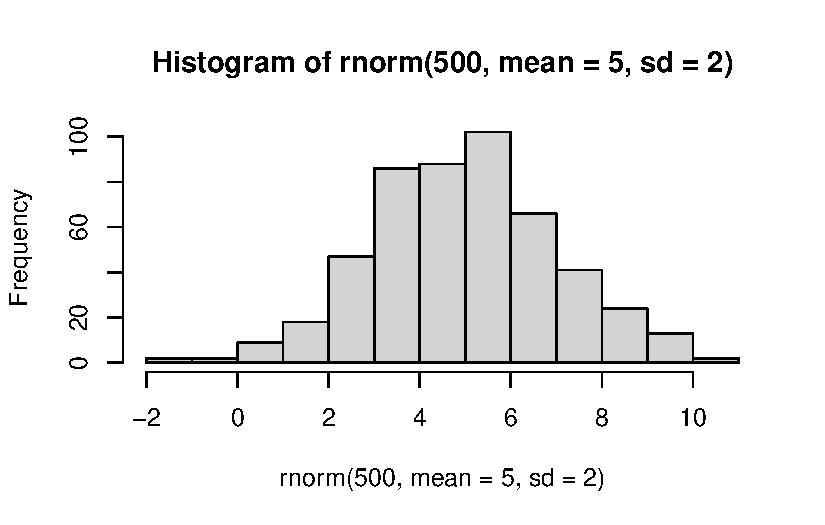
\includegraphics[keepaspectratio]{r_basics_files/figure-pdf/unnamed-chunk-19-1.pdf}}

~~~~~~Using \texttt{rnorm()}, we can create matrix and convert it into
data frame or tibble.

\begin{Shaded}
\begin{Highlighting}[]
\NormalTok{mat }\OtherTok{=} \FunctionTok{matrix}\NormalTok{(}\FunctionTok{rnorm}\NormalTok{(}\DecValTok{50}\NormalTok{), }\AttributeTok{ncol =} \DecValTok{5}\NormalTok{)}
\FunctionTok{colnames}\NormalTok{(mat) }\OtherTok{=} \FunctionTok{c}\NormalTok{(}\StringTok{"a"}\NormalTok{, }\StringTok{"b"}\NormalTok{, }\StringTok{"c"}\NormalTok{, }\StringTok{"d"}\NormalTok{, }\StringTok{"e"}\NormalTok{)}
\FunctionTok{as\_tibble}\NormalTok{(mat)}
\end{Highlighting}
\end{Shaded}

\begin{verbatim}
# A tibble: 10 x 5
         a       b       c        d       e
     <dbl>   <dbl>   <dbl>    <dbl>   <dbl>
 1 -0.338   1.21    0.128   0.891   -0.736 
 2  0.164  -0.506  -0.339   0.549   -0.0885
 3  1.07   -1.27    0.757   0.263   -0.0408
 4  1.88   -0.813  -0.0807 -0.0332  -1.25  
 5  0.272  -0.515   0.471  -1.41     0.384 
 6  1.19    1.66   -1.37   -0.0670  -0.236 
 7 -0.936  -0.316  -0.201  -1.74     2.32  
 8  1.01   -1.22   -0.521  -0.682    0.114 
 9 -0.0706  1.12   -0.776   0.339   -1.22  
10  0.424   0.0727  1.07   -0.00472 -0.962 
\end{verbatim}

~~~~~~In additon to \texttt{runif()} and \texttt{rnorm()},
\texttt{sample()} function can be used to generate random numbers.

\begin{Shaded}
\begin{Highlighting}[]
\FunctionTok{sample}\NormalTok{(}\DecValTok{0}\SpecialCharTok{:}\DecValTok{100}\NormalTok{,}\DecValTok{5}\NormalTok{)}
\end{Highlighting}
\end{Shaded}

\begin{verbatim}
[1] 26 22 49 52 78
\end{verbatim}

\begin{Shaded}
\begin{Highlighting}[]
\FunctionTok{sample}\NormalTok{(}\DecValTok{0}\SpecialCharTok{:}\DecValTok{100}\NormalTok{,}\DecValTok{5}\NormalTok{, }\AttributeTok{replace =} \ConstantTok{TRUE}\NormalTok{)}
\end{Highlighting}
\end{Shaded}

\begin{verbatim}
[1] 68 26 76 96  5
\end{verbatim}

\begin{Shaded}
\begin{Highlighting}[]
\FunctionTok{matrix}\NormalTok{(}\FunctionTok{sample}\NormalTok{(}\DecValTok{0}\SpecialCharTok{:}\DecValTok{50}\NormalTok{,}\DecValTok{50}\NormalTok{), }\AttributeTok{ncol =} \DecValTok{5}\NormalTok{)}
\end{Highlighting}
\end{Shaded}

\begin{verbatim}
      [,1] [,2] [,3] [,4] [,5]
 [1,]   21    2   24    9   39
 [2,]   23   43   41   22    1
 [3,]    8    6   44   47   33
 [4,]   16   15   36   10   12
 [5,]   27   32    0   45   25
 [6,]   11    7   28   34   35
 [7,]   46   26   48   40   20
 [8,]   49   18   14   42   17
 [9,]   38   19   50   30    3
[10,]   31   13   37    5    4
\end{verbatim}

\section{Functions}\label{functions}

~~~~~In R, there are some functions that we use very frequently. In this
section, we will discuss some of those functions.

\subsection{\texorpdfstring{\texttt{for} Loop
Function}{for Loop Function}}\label{for-loop-function-1}

~~~~~\texttt{for} loop function in R is used to iterate over\footnote{Iteration
  (also called looping) is the process of repeating the same operation
  on different columns, or on different datasets. There are two
  important iteration paradigms: \texttt{imperative\ programming} and
  \texttt{functional\ programming}. On the imperative side, one has
  tools like \texttt{for\ ()} loops and \texttt{while\ ()} loops, which
  are a great place to start because they make iteration very explicit,
  so it is obvious what is happening. However, \texttt{for\ ()} loops
  are quite verbose, and require quite a bit of bookkeeping code that is
  duplicated for every for loop. One the other hand
  \texttt{Functional\ programming\ (FP)} offers tools to extract out
  this dupli cated code, so each common \texttt{for} loop pattern gets
  its own function. Once one masters the vocabulary of FP, one can solve
  many common iteration problems with \emph{less code}, \emph{more
  ease}, and \emph{fewer errors}. The \texttt{apply\ ()} family
  functions in base R are equivalent to \texttt{for\ ()} loop. The
  \texttt{apply\ ()} family functions include the following functions
  for looping- \texttt{apply\ ()}; \texttt{lapply\ ()};
  \texttt{sapply\ ()}, \texttt{tapply\ ()}, \texttt{vapply\ ()}, and
  \texttt{mapply\ ()}. The \texttt{purrr} package in tidyverse offers
  \texttt{map\ ()} family functions for functional programming, which we
  will be using for the loop operations.} the elements of a vector, or a
list, or a matrix, or a data frame, or a tibble and apply a set of
instructions (operations) on each item of the object. \texttt{for} loop
function is used to avoid unnecessary repeition of code, thus enhancing
efficiency and effectiveness of code. The basic syntax of \texttt{for}
loop function in R -

\begin{Shaded}
\begin{Highlighting}[]
\ControlFlowTok{for}\NormalTok{ (item }\ControlFlowTok{in}\NormalTok{ object) \{}
\NormalTok{    Statement}
\NormalTok{\}}
\end{Highlighting}
\end{Shaded}

~~~~~Some examples of \texttt{for} loop function are -

\begin{Shaded}
\begin{Highlighting}[]
\ControlFlowTok{for}\NormalTok{ (x }\ControlFlowTok{in} \FunctionTok{seq}\NormalTok{(}\DecValTok{1}\SpecialCharTok{:}\DecValTok{5}\NormalTok{)) \{}
    \FunctionTok{print}\NormalTok{(x}\SpecialCharTok{\^{}}\DecValTok{2}\NormalTok{)}
\NormalTok{\}}
\end{Highlighting}
\end{Shaded}

\begin{verbatim}
[1] 1
[1] 4
[1] 9
[1] 16
[1] 25
\end{verbatim}

\begin{Shaded}
\begin{Highlighting}[]
\ControlFlowTok{for}\NormalTok{ (x }\ControlFlowTok{in} \FunctionTok{c}\NormalTok{(}\StringTok{\textquotesingle{}Adam\textquotesingle{}}\NormalTok{, }\StringTok{"Joseph"}\NormalTok{, }\StringTok{"John"}\NormalTok{)) \{}
    \FunctionTok{print}\NormalTok{(x)}
\NormalTok{\}}
\end{Highlighting}
\end{Shaded}

\begin{verbatim}
[1] "Adam"
[1] "Joseph"
[1] "John"
\end{verbatim}

\begin{Shaded}
\begin{Highlighting}[]
\CommentTok{\# Vectors for numbers and names}
\NormalTok{numbers }\OtherTok{\textless{}{-}} \DecValTok{1}\SpecialCharTok{:}\DecValTok{3}
\NormalTok{names }\OtherTok{\textless{}{-}} \FunctionTok{c}\NormalTok{(}\StringTok{\textquotesingle{}Adam\textquotesingle{}}\NormalTok{, }\StringTok{\textquotesingle{}Joseph\textquotesingle{}}\NormalTok{, }\StringTok{\textquotesingle{}John\textquotesingle{}}\NormalTok{)}

\CommentTok{\# Loop through the vectors and print the desired output}
\ControlFlowTok{for}\NormalTok{ (i }\ControlFlowTok{in} \DecValTok{1}\SpecialCharTok{:}\FunctionTok{length}\NormalTok{(numbers)) \{}
    \FunctionTok{print}\NormalTok{(}\FunctionTok{paste}\NormalTok{(numbers[i], names[i], }\AttributeTok{sep =} \StringTok{", "}\NormalTok{))}
\NormalTok{\}}
\end{Highlighting}
\end{Shaded}

\begin{verbatim}
[1] "1, Adam"
[1] "2, Joseph"
[1] "3, John"
\end{verbatim}

\subsection{\texorpdfstring{\texttt{map()}
Function}{map() Function}}\label{map-function-1}

~~~~~ In \texttt{map()} function, the purpose is to apply a
\textbf{function} on a \textbf{vector or list}, meaning that
\texttt{map()} functions take a list/vector and a function as arguments.
Figure~\ref{fig-rmap} sows the nature of \texttt{map()} function. The
\texttt{map()} function then applies the function to each element of the
\texttt{list/vector} and the result of this process is then combined
into a \texttt{list}. For example, a list called sample\_list is
created. The \texttt{length()} function can be used to know the elements
of the list. However, if you want to the element of each list, then
\texttt{map()} function can be used. The other variation of map()
functions that the package purrr include - \texttt{map\_int()},
\texttt{map\_dbl()}, \texttt{map\_chr()}, and
\texttt{map\_lgl()}\footnote{The output of \texttt{map()} function is
  always list. These variations help to get the desired output. To learn
  more about map functions, please visit -
  \url{https://adv-r.hadley.nz/functionals.html}.}.

\begin{figure}

\centering{

\pandocbounded{\includegraphics[keepaspectratio]{images/map-step-1.png}}

}

\caption{\label{fig-rmap}map() Function Argument}

\end{figure}%

\begin{Shaded}
\begin{Highlighting}[]
\NormalTok{sample\_list }\OtherTok{\textless{}{-}} 
    \FunctionTok{list}\NormalTok{(}
        \AttributeTok{x =} \FloatTok{1737.1}\NormalTok{,}
        \AttributeTok{y =} \FunctionTok{c}\NormalTok{(}\FloatTok{11.3}\NormalTok{, }\FloatTok{6.2}\NormalTok{),}
        \AttributeTok{z =} \FunctionTok{c}\NormalTok{(}\FloatTok{60.4}\NormalTok{, }\FloatTok{81.4}\NormalTok{, }\DecValTok{156}\NormalTok{, }\FloatTok{174.8}\NormalTok{, }\DecValTok{194}\NormalTok{, }\FloatTok{34.8}\NormalTok{, }\DecValTok{420}\NormalTok{, }\FloatTok{2705.2}\NormalTok{, }\DecValTok{340}\NormalTok{, }\DecValTok{62}\NormalTok{)}
\NormalTok{ )}
\NormalTok{sample\_list}
\end{Highlighting}
\end{Shaded}

\begin{verbatim}
$x
[1] 1737.1

$y
[1] 11.3  6.2

$z
 [1]   60.4   81.4  156.0  174.8  194.0   34.8  420.0 2705.2  340.0   62.0
\end{verbatim}

\begin{Shaded}
\begin{Highlighting}[]
\FunctionTok{length}\NormalTok{(sample\_list)}
\end{Highlighting}
\end{Shaded}

\begin{verbatim}
[1] 3
\end{verbatim}

\begin{Shaded}
\begin{Highlighting}[]
\FunctionTok{map}\NormalTok{(sample\_list, length)}
\end{Highlighting}
\end{Shaded}

\begin{verbatim}
$x
[1] 1

$y
[1] 2

$z
[1] 10
\end{verbatim}

\subsubsection{\texorpdfstring{\texttt{map()} Functions with Multiple
Inputs}{map() Functions with Multiple Inputs}}\label{map-functions-with-multiple-inputs}

~~~~~ The \texttt{map2()} functions are very similar to the
\texttt{map()} functions, but they take two input vectors instead of
one. Since the \texttt{map2()} functions iterate along the two vectors
in parallel, they need to be of the same length. Figure~\ref{fig-rmap2}
shows a \texttt{map2()} function.

\begin{figure}

\centering{

\pandocbounded{\includegraphics[keepaspectratio]{images/map2.png}}

}

\caption{\label{fig-rmap2}map2() Function}

\end{figure}%

\begin{Shaded}
\begin{Highlighting}[]
\NormalTok{x }\OtherTok{\textless{}{-}} \FunctionTok{c}\NormalTok{(}\DecValTok{1}\NormalTok{, }\DecValTok{2}\NormalTok{, }\DecValTok{4}\NormalTok{)}
\NormalTok{y }\OtherTok{\textless{}{-}} \FunctionTok{c}\NormalTok{(}\DecValTok{6}\NormalTok{, }\DecValTok{5}\NormalTok{, }\DecValTok{3}\NormalTok{)}
\FunctionTok{map2\_dbl}\NormalTok{(x, y, min)}
\end{Highlighting}
\end{Shaded}

\begin{verbatim}
[1] 1 2 3
\end{verbatim}

\begin{Shaded}
\begin{Highlighting}[]
\NormalTok{df }\OtherTok{\textless{}{-}}
    \FunctionTok{tibble}\NormalTok{(}
        \AttributeTok{a =} \FunctionTok{c}\NormalTok{(}\DecValTok{1}\NormalTok{, }\DecValTok{2}\NormalTok{, }\DecValTok{4}\NormalTok{),}
        \AttributeTok{b =} \FunctionTok{c}\NormalTok{(}\DecValTok{6}\NormalTok{, }\DecValTok{5}\NormalTok{, }\DecValTok{3}\NormalTok{)}
\NormalTok{        )}

\NormalTok{df }\SpecialCharTok{\%\textgreater{}\%}
    \FunctionTok{mutate}\NormalTok{(}\AttributeTok{min =} \FunctionTok{map2\_dbl}\NormalTok{(a, b, min))}
\end{Highlighting}
\end{Shaded}

\begin{verbatim}
# A tibble: 3 x 3
      a     b   min
  <dbl> <dbl> <dbl>
1     1     6     1
2     2     5     2
3     4     3     3
\end{verbatim}

\begin{Shaded}
\begin{Highlighting}[]
\NormalTok{df }\SpecialCharTok{\%\textgreater{}\%}
    \FunctionTok{mutate}\NormalTok{(}
        \AttributeTok{min =} \FunctionTok{min}\NormalTok{(a,b)}
\NormalTok{        )}
\end{Highlighting}
\end{Shaded}

\begin{verbatim}
# A tibble: 3 x 3
      a     b   min
  <dbl> <dbl> <dbl>
1     1     6     1
2     2     5     1
3     4     3     1
\end{verbatim}

~~~~~ By default \texttt{mutate()}, uses column-wise operations.
\texttt{map2\_dbl()} produces a column the same length at \texttt{a} and
\texttt{b}. We can accomplish the same calculation using
\texttt{row-wise} operations.

\begin{Shaded}
\begin{Highlighting}[]
\NormalTok{ df }\SpecialCharTok{\%\textgreater{}\%}
    \FunctionTok{rowwise}\NormalTok{() }\SpecialCharTok{\%\textgreater{}\%}
    \FunctionTok{mutate}\NormalTok{(}\AttributeTok{min =} \FunctionTok{min}\NormalTok{(a, b)) }\SpecialCharTok{\%\textgreater{}\%}
    \FunctionTok{ungroup}\NormalTok{()}
\end{Highlighting}
\end{Shaded}

\begin{verbatim}
# A tibble: 3 x 3
      a     b   min
  <dbl> <dbl> <dbl>
1     1     6     1
2     2     5     2
3     4     3     3
\end{verbatim}

\subsubsection{\texorpdfstring{\texttt{pmap()}
Functions}{pmap() Functions}}\label{pmap-functions}

~~~~~ There are no \texttt{map3()} or \texttt{map4()} functions.
Instead, you can use a \texttt{pmap()} (\emph{p} for \emph{parallel})
function to map over more than two vectors. The \texttt{pmap()}
functions work slightly differently than the \texttt{map()} and
\texttt{map2()} functions. In \texttt{map()} and \texttt{map2()}
functions, you specify the \texttt{vector(s)} to supply to the function.
In \texttt{pmap()} functions, you specify a single \texttt{list} that
contains all the vectors (or lists) that you want to supply to your
function. Figure~\ref{fig-rpmap} shows a \texttt{pmap()} function.

\begin{figure}

\centering{

\pandocbounded{\includegraphics[keepaspectratio]{images/pmap-list.png}}

}

\caption{\label{fig-rpmap}pmap() Function (List)}

\end{figure}%

~~~~~ Flipping the list diagram makes it easier to see that
\texttt{pmap()} is basically just a generalized version of
\texttt{map2()} (See Figure~\ref{fig-rpmapfilip}).

\begin{figure}

\centering{

\pandocbounded{\includegraphics[keepaspectratio]{images/pmap-flipped.png}}

}

\caption{\label{fig-rpmapfilip}pmap() Function (Flipped)}

\end{figure}%

~~~~~ The only difference is that \texttt{map2()} lets you specify each
vector as a separate argument. In \texttt{pmap()}, you have to store all
your input vectors in a single list. This functionality allows
\texttt{pmap()} to handle any number of input vectors.

\begin{Shaded}
\begin{Highlighting}[]
\NormalTok{x }\OtherTok{\textless{}{-}} \FunctionTok{c}\NormalTok{(}\DecValTok{1}\NormalTok{, }\DecValTok{2}\NormalTok{, }\DecValTok{4}\NormalTok{)}
\NormalTok{y }\OtherTok{\textless{}{-}} \FunctionTok{c}\NormalTok{(}\DecValTok{6}\NormalTok{, }\DecValTok{5}\NormalTok{, }\DecValTok{3}\NormalTok{)}
\FunctionTok{map2\_dbl}\NormalTok{(x, y, min)}
\end{Highlighting}
\end{Shaded}

\begin{verbatim}
[1] 1 2 3
\end{verbatim}

\begin{Shaded}
\begin{Highlighting}[]
\FunctionTok{pmap\_dbl}\NormalTok{(}\FunctionTok{list}\NormalTok{(x, y), min)}
\end{Highlighting}
\end{Shaded}

\begin{verbatim}
[1] 1 2 3
\end{verbatim}

\begin{Shaded}
\begin{Highlighting}[]
\NormalTok{z }\OtherTok{\textless{}{-}} \FunctionTok{c}\NormalTok{(}\DecValTok{100}\NormalTok{, }\DecValTok{15}\NormalTok{, }\DecValTok{1}\NormalTok{)}
\FunctionTok{pmap\_dbl}\NormalTok{(}\FunctionTok{list}\NormalTok{(x, y, z), max)}
\end{Highlighting}
\end{Shaded}

\begin{verbatim}
[1] 100  15   4
\end{verbatim}

\subsection{User Defined Functions}\label{user-defined-functions}

~~~~~ User defined functions are also called named functions because
they are assigned a name and expected to be called frequently. The goal
of user defined functions is to optimize program, avoid or minimize the
reptition of the code, prevent errors, and make the code more readable.
In R, to declare a user defined function, we use the keywoard
\texttt{function()}. The syntax of user defined function is given below.
It is clear that there are three components of an R function -
\textbf{function name}, \textbf{function parameters (arguments)}, and
\textbf{function body (expression)}. We can drop curly braces
(\texttt{\{\}}) from the function if the function body contains a single
statement. Moreover, the function must be called with the correct number
of arguments.

\begin{Shaded}
\begin{Highlighting}[]
\NormalTok{functionname }\OtherTok{=} \ControlFlowTok{function}\NormalTok{ (arguments) \{}
    \ControlFlowTok{function}\NormalTok{ body }
\NormalTok{\}}
\end{Highlighting}
\end{Shaded}

~~~~~ Below are examples of some user defined functions.

\begin{Shaded}
\begin{Highlighting}[]
\NormalTok{add\_numbers }\OtherTok{=} \ControlFlowTok{function}\NormalTok{ (x,y)\{}
\NormalTok{    sum }\OtherTok{=}\NormalTok{ x }\SpecialCharTok{+}\NormalTok{ y }
    \FunctionTok{return}\NormalTok{(sum)}
\NormalTok{\}}
\FunctionTok{add\_numbers}\NormalTok{(}\DecValTok{5}\NormalTok{,}\SpecialCharTok{{-}}\DecValTok{25}\NormalTok{)}
\end{Highlighting}
\end{Shaded}

\begin{verbatim}
[1] -20
\end{verbatim}

\begin{Shaded}
\begin{Highlighting}[]
\NormalTok{greetings }\OtherTok{=} \ControlFlowTok{function}\NormalTok{ (name, }\AttributeTok{greeting =} \StringTok{"Welcome"}\NormalTok{, }\AttributeTok{sign =} \StringTok{"!"}\NormalTok{)\{}
\NormalTok{    greetingtogether }\OtherTok{=} \FunctionTok{paste}\NormalTok{(name, sign, }\AttributeTok{sep =} \StringTok{""}\NormalTok{)}
    \FunctionTok{print}\NormalTok{(}\FunctionTok{paste}\NormalTok{(greeting, greetingtogether))}
\NormalTok{\}}
\FunctionTok{greetings}\NormalTok{(}\StringTok{"Nicole"}\NormalTok{)}
\end{Highlighting}
\end{Shaded}

\begin{verbatim}
[1] "Welcome Nicole!"
\end{verbatim}

\subsection{Anonymous Functions}\label{anonymous-functions}

~~~~~ Anonymous functions are functions that are not named, meaning that
unlike normal functions, they do not have any name. Anonymous functions
are useful when we do not plan to use them again and again. In most
cases, we use anonymous function as an argument to other functions. In
R, the synax of anonymous function is very much similar to named
function. The syntax of anonymous function is -
\texttt{function\ (x)\ expression}.

\begin{Shaded}
\begin{Highlighting}[]
\NormalTok{vec }\OtherTok{=} \FunctionTok{c}\NormalTok{ (}\DecValTok{1}\NormalTok{,}\DecValTok{5}\NormalTok{,}\DecValTok{6}\NormalTok{)}
\FunctionTok{sapply}\NormalTok{(vec, }\ControlFlowTok{function}\NormalTok{(x) x}\SpecialCharTok{\^{}}\DecValTok{2}\NormalTok{)}
\end{Highlighting}
\end{Shaded}

\begin{verbatim}
[1]  1 25 36
\end{verbatim}

~~~~~ Sometimes, using \texttt{purrr}, we can create anonymous function
by one sided formula. In the below example,
\texttt{\textasciitilde{}.x**2} works like \texttt{function\ (x)\ x**2}.

\begin{Shaded}
\begin{Highlighting}[]
\FunctionTok{map\_int}\NormalTok{(}\DecValTok{1}\SpecialCharTok{:}\DecValTok{5}\NormalTok{, }\SpecialCharTok{\textasciitilde{}}\NormalTok{.x}\SpecialCharTok{**}\DecValTok{2}\NormalTok{)}
\end{Highlighting}
\end{Shaded}

\begin{verbatim}
[1]  1  4  9 16 25
\end{verbatim}

\section{Conclusions}\label{conclusions-3}

\section*{Exercises}\label{exercises-3}
\addcontentsline{toc}{section}{Exercises}

\markright{Exercises}

\chapter{Chapter 1 Solution}\label{chapter-1-solution}

\chapter{Chapter 2 Solution}\label{chapter-2-solution}

\chapter*{References}\label{references}
\addcontentsline{toc}{chapter}{References}

\markboth{References}{References}

\protect\phantomsection\label{refs}
\begin{CSLReferences}{1}{1}
\bibitem[\citeproctext]{ref-alles_drivers_2015}
Alles, Michael. 2015. {``Drivers of the Use and Facilitators and
Obstacles of the Evolution of Big Data by the Audit Profession.''}
\emph{Accounting Horizons} 29 (2): 439--49.
\url{https://publications.aaahq.org/accounting-horizons/article-abstract/29/2/439/2188}.

\bibitem[\citeproctext]{ref-alles_incorporating_2016}
Alles, Michael, and Glen Gray. 2016. {``Incorporating Big Data in
Audits: {Identifying} Inhibitors and a Research Agenda to Address Those
Inhibitors.''} \emph{International Journal of Accounting Information
Systems} 22: 44--59.
\url{https://www.sciencedirect.com/science/article/pii/S1467089516300811}.

\bibitem[\citeproctext]{ref-american_institute_of_certified_public_accountants_aicpa_audit_2015}
American Institute of Certified Public Accountants (AICPA). 2015.
\emph{Audit {Analytics} and {Continuous} {Audit}: {Looking} {Toward} the
{Future}}.

\bibitem[\citeproctext]{ref-american_institute_of_certified_public_accountants_aicpa_description_2017}
American Institute of Certified Public Accountants (AICPA). 2017.
\emph{Description {Criteria} for {Management}'s {Description} of the
{Entity}'s {Cybersecurity} {Risk} {Management} {Program}}.

\bibitem[\citeproctext]{ref-appelbaum_securing_2016}
Appelbaum, Deniz. 2016. {``Securing Big Data Provenance for Auditors:
{The} Big Data Provenance Black Box as Reliable Evidence.''}
\emph{Journal of Emerging Technologies in Accounting} 13 (1): 17--36.
\url{https://publications.aaahq.org/jeta/article-abstract/13/1/17/9219}.

\bibitem[\citeproctext]{ref-appelbaum_big_2017}
Appelbaum, Deniz, Alexander Kogan, and Miklos A. Vasarhelyi. 2017.
{``Big {Data} and Analytics in the Modern Audit Engagement: {Research}
Needs.''} \emph{Auditing: A Journal of Practice \& Theory} 36 (4):
1--27.
\url{https://publications.aaahq.org/ajpt/article-abstract/36/4/1/6016}.

\bibitem[\citeproctext]{ref-barr-pulliam_audit_2023}
Barr-Pulliam, Dereck, Helen L. Brown-Liburd, and Amanda G. Carlson.
2023. {``Do {Audit} {Data} {Analytics} {Influence} {Juror} {Perceptions}
of {Audit} {Quality} and {Auditor} {Negligence}?''} \emph{Current Issues
in Auditing} 17 (2): P1--10.
\url{https://publications.aaahq.org/cia/article/17/2/P1/10096}.

\bibitem[\citeproctext]{ref-barton_making_2012}
Barton, Dominic, and David Court. 2012. {``Making Advanced Analytics
Work for You.''} \emph{Harvard Business Review} 90 (10): 78--83.
\url{http://www.buyukverienstitusu.com/s/1870/i/Making_Advanced_Analytics_Work_For_You.pdf}.

\bibitem[\citeproctext]{ref-bollen_twitter_2011}
Bollen, Johan, Huina Mao, and Xiaojun Zeng. 2011. {``Twitter Mood
Predicts the Stock Market.''} \emph{Journal of Computational Science} 2
(1): 1--8.
\url{https://www.sciencedirect.com/science/article/pii/S187775031100007X}.

\bibitem[\citeproctext]{ref-cao_big_2015}
Cao, Min, Roman Chychyla, and Trevor Stewart. 2015. {``Big Data
Analytics in Financial Statement Audits.''} \emph{Accounting Horizons}
29 (2): 423--29.
\url{https://publications.aaahq.org/accounting-horizons/article-abstract/29/2/423/2177}.

\bibitem[\citeproctext]{ref-columbus_53_2017}
Columbus. 2017. {``53\% {Of} {Companies} {Are} {Adopting} {Big} {Data}
{Analytics}.''} \emph{Forbes}.
\url{https://www.forbes.com/sites/louiscolumbus/2017/12/24/53-of-companies-are-adopting-big-data-analytics/?sh=6c98f39939a1}.

\bibitem[\citeproctext]{ref-crawley_analytics_2014}
Crawley, Michael, and James Wahlen. 2014. {``Analytics in
Empirical/Archival Financial Accounting Research.''} \emph{Business
Horizons} 57 (5): 583--93.
\url{https://www.sciencedirect.com/science/article/pii/S0007681314000792}.

\bibitem[\citeproctext]{ref-dai_imagineering_2016}
Dai, Jun, and Miklos A. Vasarhelyi. 2016. {``Imagineering {Audit}
4.0.''} \emph{Journal of Emerging Technologies in Accounting} 13 (1):
1--15.
\url{https://publications.aaahq.org/jeta/article-abstract/13/1/1/9242}.

\bibitem[\citeproctext]{ref-davis_beyond_2012}
Davis, Angela K., Jeremy M. Piger, and Lisa M. Sedor. 2012. {``Beyond
the {Numbers}: {Measuring} the {Information} {Content} of {Earnings}
{Press} {Release} {Language}.''} \emph{Contemporary Accounting Research}
29 (3): 845--68. \url{https://doi.org/10.1111/j.1911-3846.2011.01130.x}.

\bibitem[\citeproctext]{ref-deloitte_tax_2016}
Deloitte. 2016. \emph{Tax {Data} {Analytics} {A} {New} {Era} for {Tax}
{Planning} and {Compliance}}.
\url{https://www2.deloitte.com/content/dam/Deloitte/us/Documents/Tax/us-tax-data-analytics-a-new-era-for-tax-planning-and-compliance.pdf}.

\bibitem[\citeproctext]{ref-deloitte2024industryadvantage}
Deloitte. 2024. \emph{Deloitte Invests \$2 Billion to Accelerate
IndustryAdvantage™ for Its Clients}.
\url{https://www2.deloitte.com/us/en/pages/about-deloitte/articles/press-releases/deloitte-invests-two-billion-to-accelerate-industryadvantage-for-its-clients.html}.

\bibitem[\citeproctext]{ref-estep2024financial}
Estep, Cassandra, Emily E Griffith, and Nikki L MacKenzie. 2024. {``How
Do Financial Executives Respond to the Use of Artificial Intelligence in
Financial Reporting and Auditing?''} \emph{Review of Accounting Studies}
29 (3): 2798--831.

\bibitem[\citeproctext]{ref-ey2023ai}
EY. 2023. \emph{EY Announces Launch of Artificial Intelligence Platform
EY.ai Following US\$1.4b Investment}.
\url{https://www.ey.com/en_gl/newsroom/2023/09/ey-announces-launch-of-artificial-intelligence-platform-ey-ai-following-us-1-4b-investment}.

\bibitem[\citeproctext]{ref-fedyk2022artificial}
Fedyk, Anastassia, James Hodson, Natalya Khimich, and Tatiana Fedyk.
2022. {``Is Artificial Intelligence Improving the Audit Process?''}
\emph{Review of Accounting Studies} 27 (3): 938--85.

\bibitem[\citeproctext]{ref-feldman_managements_2010}
Feldman, Ronen, Suresh Govindaraj, Joshua Livnat, and Benjamin Segal.
2010. {``Management's Tone Change, Post Earnings Announcement Drift and
Accruals.''} \emph{Review of Accounting Studies} 15 (4): 915--53.
\url{https://doi.org/10.1007/s11142-009-9111-x}.

\bibitem[\citeproctext]{ref-sahota2024dawn}
Forbes. 2024. \emph{The Dawn of a New Era: AI's Revolutionary Role in
Accounting}.
\url{https://www.forbes.com/sites/neilsahota/2024/04/22/the-dawn-of-a-new-era-ais-revolutionary-role-in-accounting/?sh=1ff4bc4858af}.

\bibitem[\citeproctext]{ref-krahel_consequences_2015}
Krahel, John Peter, and William R. Titera. 2015. {``Consequences of Big
Data and Formalization on Accounting and Auditing Standards.''}
\emph{Accounting Horizons} 29 (2): 409--22.
\url{https://publications.aaahq.org/accounting-horizons/article/29/2/409/2149}.

\bibitem[\citeproctext]{ref-lehavy_effect_2011}
Lehavy, Reuven, Feng Li, and Kenneth Merkley. 2011. {``The Effect of
Annual Report Readability on Analyst Following and the Properties of
Their Earnings Forecasts.''} \emph{The Accounting Review} 86 (3):
1087--115.
\url{https://publications.aaahq.org/accounting-review/article-abstract/86/3/1087/3300}.

\bibitem[\citeproctext]{ref-li_annual_2008}
Li, Feng. 2008. {``Annual Report Readability, Current Earnings, and
Earnings Persistence.''} \emph{Journal of Accounting and Economics} 45
(2-3): 221--47.
\url{https://www.sciencedirect.com/science/article/pii/S0165410108000141}.

\bibitem[\citeproctext]{ref-li_information_2010}
Li, Feng. 2010. {``The {Information} {Content} of {Forward}‐{Looking}
{Statements} in {Corporate} {Filings}---{A} {Naïve} {Bayesian} {Machine}
{Learning} {Approach}.''} \emph{Journal of Accounting Research} 48 (5):
1049--102. \url{https://doi.org/10.1111/j.1475-679X.2010.00382.x}.

\bibitem[\citeproctext]{ref-li_measure_2013}
Li, Feng, Russell Lundholm, and Michael Minnis. 2013. {``A {Measure} of
{Competition} {Based} on 10‐{K} {Filings}.''} \emph{Journal of
Accounting Research} 51 (2): 399--436.
\url{https://doi.org/10.1111/j.1475-679X.2012.00472.x}.

\bibitem[\citeproctext]{ref-loten2023pwc}
Loten, Angus. 2023. \emph{PricewaterhouseCoopers to Pour \$1 Billion
into Generative AI}.
\url{https://www.wsj.com/articles/pricewaterhousecoopers-to-pour-1-billion-into-generative-ai-cac2cedd}.

\bibitem[\citeproctext]{ref-persico2017ai}
{Persico, F, H Sidhu, et al.} 2017. {``How AI Will Turn Auditors into
Analysts.''} \emph{Accounting Today}.
\url{https://www.accountingtoday.com/opinion/how-ai-will-turn-auditors-into-analysts}.

\bibitem[\citeproctext]{ref-protiviti_embracing_2017}
Protiviti. 2017. \emph{Embracing {Analytics} in {Auditing}}.
\url{https://www.protiviti.com/sites/default/files/2022-06/2017-internal-audit-capabilities-and-needs-survey-protiviti.pdf}.

\bibitem[\citeproctext]{ref-provost_data_2013}
Provost, Foster, and Tom Fawcett. 2013. {``Data {Science} and Its
{Relationship} to {Big} {Data} and {Data}-{Driven} {Decision}
{Making}.''} \emph{Big Data} 1 (1): 51--59.
\url{https://doi.org/10.1089/big.2013.1508}.

\bibitem[\citeproctext]{ref-raschka2022machine}
Raschka, Sebastian, Yuxi (Hayden) Liu, and Vahid Mirjalili. 2022.
\emph{Machine Learning with PyTorch and Scikit-Learn: Develop Machine
Learning and Deep Learning Models with Python}. Packt Publishing.
\url{https://books.google.com/books/about/Machine_Learning_with_PyTorch_and_Scikit.html?id=SVxaEAAAQBAJ}.

\bibitem[\citeproctext]{ref-reddy2025}
Reddi, Vijay. 2025. \emph{Machine Learning Systems}. "Creative Commons".
\url{https://mlsysbook.ai/}.

\bibitem[\citeproctext]{ref-rhys2020machine}
Rhys, Hefin. 2020. \emph{Machine Learning with r, the Tidyverse, and
Mlr}. Simon; Schuster.

\bibitem[\citeproctext]{ref-richins_big_2017}
Richins, Greg, Andrea Stapleton, Theophanis C. Stratopoulos, and
Christopher Wong. 2017. {``Big Data Analytics: Opportunity or Threat for
the Accounting Profession?''} \emph{Journal of Information Systems} 31
(3): 63--79.
\url{https://publications.aaahq.org/jis/article-abstract/31/3/63/1114}.

\bibitem[\citeproctext]{ref-rose_when_2017}
Rose, Anna M., Jacob M. Rose, Kerri-Ann Sanderson, and Jay C. Thibodeau.
2017. {``When Should Audit Firms Introduce Analyses of Big Data into the
Audit Process?''} \emph{Journal of Information Systems} 31 (3): 81--99.
\url{https://publications.aaahq.org/jis/article-abstract/31/3/81/1123}.

\bibitem[\citeproctext]{ref-schatsky16cognitive}
Schatsky, D, C Muraskin, and G Ragu. 2015. \emph{Cognitive Technologies:
The Real Opportunities for Business}.
\url{https://www2.deloitte.com/us/en/insights/deloitte-review/issue-16/cognitive-technologies-business-applications.html}.

\bibitem[\citeproctext]{ref-schneider_infer_2015}
Schneider, Gary P., Jun Dai, Diane J. Janvrin, Kemi Ajayi, and Robyn L.
Raschke. 2015. {``Infer, Predict, and Assure: {Accounting} Opportunities
in Data Analytics.''} \emph{Accounting Horizons} 29 (3): 719--42.
\url{https://publications.aaahq.org/accounting-horizons/article-abstract/29/3/719/2262}.

\bibitem[\citeproctext]{ref-sivarajah_critical_2017}
Sivarajah, Uthayasankar, Muhammad Mustafa Kamal, Zahir Irani, and
Vishanth Weerakkody. 2017. {``Critical Analysis of {Big} {Data}
Challenges and Analytical Methods.''} \emph{Journal of Business
Research} 70: 263--86.
\url{https://www.sciencedirect.com/science/article/pii/S014829631630488X}.

\bibitem[\citeproctext]{ref-the_economist_worlds_2017}
The Economist. 2017. \emph{The World's Most Valuable Resource Is No
Longer Oil, but Data}.
\url{https://www.economist.com/leaders/2017/05/06/the-worlds-most-valuable-resource-is-no-longer-oil-but-data}.

\bibitem[\citeproctext]{ref-vasarhelyi_big_2015}
Vasarhelyi, Miklos A., Alexander Kogan, and Brad M. Tuttle. 2015. {``Big
Data in Accounting: {An} Overview.''} \emph{Accounting Horizons} 29 (2):
381--96.
\url{https://publications.aaahq.org/accounting-horizons/article-abstract/29/2/381/2184}.

\bibitem[\citeproctext]{ref-verver_six_2015}
Verver, John. 2015. {``Six {Audit} {Analytics} {Success} {Factors}.''}
\emph{Internal Auditor} 72 (3).

\bibitem[\citeproctext]{ref-vien2018drone}
Vien, Courtney. 2018. {``Using Drones to Enhance Audit.''} \emph{Journal
of Accountancy}.
\url{https://www.journalofaccountancy.com/podcast/using-drones-to-enhance-audits.html}.

\bibitem[\citeproctext]{ref-warren_how_2015}
Warren, J. Donald, Kevin C. Moffitt, and Paul Byrnes. 2015. {``How Big
Data Will Change Accounting.''} \emph{Accounting Horizons} 29 (2):
397--407.
\url{https://publications.aaahq.org/accounting-horizons/article/29/2/397/2168}.

\bibitem[\citeproctext]{ref-wickham2023r}
Wickham, Hadley, Mine Çetinkaya-Rundel, and Garrett Grolemund. 2023.
\emph{R for Data Science}. " O'Reilly Media, Inc.".
\url{https://r4ds.hadley.nz/}.

\bibitem[\citeproctext]{ref-yoon_big_2015}
Yoon, Kyunghee, Lucas Hoogduin, and Li Zhang. 2015. {``Big Data as
Complementary Audit Evidence.''} \emph{Accounting Horizons} 29 (2):
431--38.
\url{https://publications.aaahq.org/accounting-horizons/article/29/2/431/2215}.

\bibitem[\citeproctext]{ref-zhang_toward_2015}
Zhang, Juan, Xiongsheng Yang, and Deniz Appelbaum. 2015. {``Toward
Effective Big Data Analysis in Continuous Auditing.''} \emph{Accounting
Horizons} 29 (2): 469--76.
\url{https://publications.aaahq.org/accounting-horizons/article/29/2/469/2160}.

\end{CSLReferences}




\end{document}
